	%to force start on odd page
	\newpage
	\thispagestyle{empty}
	\mbox{} 
	\section{Functional Analysis}\label{functional analysis}
\lettrine[lines=4]{\color{BrickRed}F}{unctional analysis} is the branch of mathematics and specifically of the analysis that is related to the study of function spaces. It takes its historical roots in the study of transformations such as the Fourier transform and in the study of differential equations and integrals. As such it encompasses so many areas that it is difficult to justify that it be a section of this book because it is rather a field of study. Moreover, it is because of this difficulty to accurately identify the area it covers that the reader will find the Fundamental Theorem of Calculus in the chapter of Integral and Differential Calculus rather than here... 
	
	Why do we use the term "analysis" in the particular case of functions? The reason lies in the historical study of various phenomena of nature and resolution of various technical problems and therefore mathematics, which often lead us to consider the variation of a parameter correlated with the variation of another or several other variables. To study these variations, many tools are available to each of us:
	\begin{itemize}
		\item The engineer, for example, frequently use charts (in cartesian, polar or logarithmic coordinate system... concepts which are discussed further in more detail) to determine the mathematical relations (or "law") linking variables between them. Certainly, this kind of method is (sometimes ...) aesthetic but students know well how it is sometimes painful to transcribe measures points on a sheet of paper or on a computer and consultants know how dangerous can be a chart when not build in a scientific way. This is unfortunately a necessary step (but should avoid an abusive usage) to understand how our predecessors worked and got the results that help us today in our advances in theoretical physics.
		
		\item The mathematician and theoretical physicist usually hate to use the paper-pencil-scrawl methods. Nevertheless, the role of the mathematician or physicist is to develop new theories with mathematical axioms or principles which should require no usage of graphical representation nor access to experimental  measures that are often attached to it.
	\end{itemize}

	\begin{tcolorbox}[title=Remark,arc=10pt,breakable,drop lifted shadow,
  skin=enhanced,
  skin first is subskin of={enhancedfirst}{arc=10pt,no shadow},
  skin middle is subskin of={enhancedmiddle}{arc=10pt,no shadow},
  skin last is subskin of={enhancedlast}{drop lifted shadow}]
Before starting to read what follows, it may be useful to remind the reader that the definition of the concept of "function" (and the basic properties thereto) is given in the section on Set Theory at page \pageref{functions and applications}.
	\end{tcolorbox}	

	Function analysis is also strongly linked to Vector Calculus (and not only...). Thus for people who want to increase their knowledge about the fundamentals of function analysis we strongly recommend the reader to have a look to the Vector Calculus section at page \pageref{vector calculus}.

\pagebreak
\subsection{Representations}

	We will see in what follows, firstly, how to represent different values related by tables and charts (yes! We must because it helps to understand more complicated stuff) and secondly how to mathematically analyse the properties of these representations only by using abstract mathematical tools.

	\textbf{Definition (\#\thesection.\mydef):} A function is named "\NewTerm{univalent function}\index{univalent function}" or  "\NewTerm{unary function}\index{unary function}" if the number of its arguments (parameters or variables) is equal to one. In the case of a function of two arguments, we speak about a "\NewTerm{bivalent function}\index{bivalent function}" or "\NewTerm{bivalent function}\index{bivalent function}", etc. Formally a function is $n$-ary if:
	

	\subsubsection{Tabular Representations}
	Among the possible visual representation of functions, the most intuitive and the oldest is the one where we have in the columns or the rows of a table in an orderly way the values of the independent variable $x_1,x_2,\ldots ,x_n$ and the corresponding values, namely the "\NewTerm{transformed variables}\index{transformed variables}" of the function $y_1,y_2,\ldots ,y_n$ in another column or aligned row:
	\begin{table}[H]
		\centering
		\definecolor{gris}{gray}{0.85}
			\begin{tabular}{|p{2cm}|p{2.5cm}|}
				\hline
				\multicolumn{1}{c}{\cellcolor[gray]{0.75}$x$} & 
  \multicolumn{1}{c}{\cellcolor[gray]{0.75}$y=f(x)$}\\ \hline
				\centering\arraybackslash\ $x_1$ & \centering\arraybackslash\ $y_1=f(x_1)$ \\ \hline
				\centering\arraybackslash\ $x_2$ & \centering\arraybackslash\ $y_2=f(x_2)$ \\ \hline
				\centering\arraybackslash\ $\ldots$ & \centering\arraybackslash\ $\ldots$ \\ \hline
				\centering\arraybackslash\ $x_n$ & \centering\arraybackslash\ $y_n=f(x_n)$ \\ \hline
		\end{tabular}
	\end{table}
	In the expression:
	
	we say that the $a_1,a_2,\ldots ,a_n$ are the "\NewTerm{arguments}\index{arguments}" of $f$ and such a table where every variable/argument is stored in a column is named a "\NewTerm{long format table}\index{long format table}".
	
	Such are, for example, tables of trigonometric functions, logarithmic tables, etc. and during the experimental study of certain phenomena tables which express the existing functional dependence between the measured physical quantities such as the readings of the temperature of the air stored in a meteorological station during one day.

	Of course, this concept can be generalized to any multivariate function regardless its definition domain.

	However, this method is laborious and does not permit to directly see the behaviour of the function and therefore a simple and attractive visual analysis of its qualitative properties for humans. It still has the advantage of not requiring any special tools or advanced mathematics and easily tractable by computers\footnote{According to the US Open Data Act. of January 12019 (holocene calendar): «\textit{\NewTerm{machine readable data} is a format that can be easily processed by a computer without human intervention while ensuring no semantic meaning is lost.}»}.
	
	Another type of tabular representation are "\NewTerm{crossed-tables}\index{crossed-tables}", also named "\NewTerm{pivot-tables}\index{pivot-tables}" or "\NewTerm{wide format}\index{wide format}",where we have categorical/ordinal variables names in the first column AND in the first row:
	\begin{table}[H] 
		\centering  
		\begin{tabular}{|l|rrr|}\hline   
		\rowcolor[gray]{0.75}& \textbf{Express Passenger} & \textbf{Ordinary Passenger} & \textbf{Total}\\    \hline    \textbf{Arriva Trains Wales}  & $3,079$ & $830$ & $3,909$\\   \textbf{Cross Country}  & $22,865$ & $63$ & $22,928$\\  \textbf{London Midland}  & $14,487$ & $33,792$ & $48,279$\\  \textbf{Virgin Trains}  & $8,594$ &  & $8,594$\\   \textbf{Total}  & $49,025$ & $34,685$ & $83,710$\\    \hline 
		\end{tabular}
	\end{table}
	And here another kind of such table but with multiple categorical column variables (the same can be done with by having multiple row variables):
	\begin{table}[H] 
		\centering
		\resizebox{\textwidth}{!}{
		\begin{tabular}{|l|rr|rr|rr|}\hline 
		\rowcolor[gray]{0.75}& \multicolumn{2}{|c|}{ \textbf{Express Passenger} } & \multicolumn{2}{|c|}{ \textbf{Ordinary Passenger} } & \multicolumn{2}{|c|}{ \textbf{Total} } \\
		\rowcolor[gray]{0.75}\cline { 2 - 7 } & \# \textbf{Trains} & \textbf{Max. Speed} & \# \textbf{Trains} & \textbf{Max. Speed} & \# \textbf{Trains} & \textbf{Max. Speed} \\
	\hline\textbf{Arriva Trains Wales} & $3,079$ & $90$ & $830$ & $90$ & $3,909$ & $90$ \\
	\textbf{Cross Country} & $22,865$ & $125$ & $63$ & $100$ & $22,928$ & $125$ \\
	\textbf{London Midland} & $14,487$ & $110$ & $33,792$ & $100$ & $48,279$ & $110$ \\
	\textbf{Virgin Trains} & $85,94$ & $125$ & & & $8,594$ & $125$ \\
	\textbf{Total} & $49,025$ & $125$ & $34,685$ & $100$ & $83,710$ & $125$ \\
	\hline
		\end{tabular}}
	\end{table}
	We can find more complex versions of the above example, like the generic multi-dimensional crossed-table with subtotals visible at page \pageref{multi-dimensional crossed-table with subtotals}.
	
	When we have a collection of repeated observations of the same subjects, taken from a given population, over some time, we speak then of "\NewTerm{longitudinal table}\index{longitudinal table}". Typically (the years are given based on the holocene calendar):
	\begin{table}[H] 
		\centering
		\begin{tabular}{|l|rrr|}\hline 
		\rowcolor[gray]{0.75}  & \textbf{January 12001} & \textbf{February 12001} & \textbf{Total}\\ \hline \textbf{Arriva Trains Wales}  & $3,079$ & $830$ & $3,909$\\ \textbf{Cross Country}  & $22,865$ & $63$ & $22,928$\\  \textbf{London Midland}  & $14,487$ & $33,792$ & $48,279$\\ \textbf{Virgin Trains}  & $8,594$ &  & $8,594$\\ \textbf{Total}  & $49,025$ & $34,685$ & $83,710$\\ \hline 
		\end{tabular}
	\end{table}
	We can have obviously also "longitudinal crossed tables", also named "longitudinal pivot tables":
	\begin{table}[H] 
		\centering  
		\resizebox{\textwidth}{!}{
		\begin{tabular}{|l|rr|rr|rr|}\hline 
		\rowcolor[gray]{0.75} & \multicolumn{2}{|c|}{ \textbf{January 12001} } & \multicolumn{2}{|c|}{\textbf{February 12001}} & \multicolumn{2}{|c|}{\textbf{Total}} \\
		\rowcolor[gray]{0.75}\cline { 2 - 7 } & \# \textbf{Trains} & \textbf{Max. Speed} & \# \textbf{Trains} & \textbf{Max. Speed} & \# \textbf{Trains} & \textbf{Max. Speed} \\
	\hline\textbf{Arriva Trains Wales} & $3,079$ & $90$ & $830$ & $90$ & $3,909$ & $90$ \\
	\textbf{Cross Country} & $22,865$ & $125$ & $63$ & $100$ & $22,928$ & $125$ \\
	\textbf{London Midland} & $14,487$ & $110$ & $33,792$ & $100$ & $48,279$ & $110$ \\
	\textbf{Virgin Trains} & $8,594$ & $125$ & & & $8,594$ & $125$ \\
	\textbf{Total} & $49,025$ & $125$ & $34,685$ & $100$ & $83,710$ & $125$ \\
	\hline
		\end{tabular}}
	\end{table}
	But all crossed and longitudinal tables (i.e. "wide formats") above are not tractable in the field of science and engineering and therefore should never be used to store datas!!! So it is common to unpivot the columns to get a normalized version of the datas (including the dates at the ISO 8601 format and removing the totals and subtotals and all fancy formatting on numerical values). The previous table, for example, will once unpivoted become the following "long format" table (i.e. "flat table"):
	\begin{table}[H]
		\centering
		\definecolor{gris}{gray}{0.85}
		\begin{tabular}{|c|c|c|c|c|}
			\hline
			\multicolumn{1}{c}{\cellcolor[gray]{0.75}\textbf{Type}} & 
  \multicolumn{1}{c}{\cellcolor[gray]{0.75}\textbf{Date}} & 
  \multicolumn{1}{c}{\cellcolor[gray]{0.75}\textbf{\# Trains}} & 
  \multicolumn{1}{c}{\cellcolor[gray]{0.75}\textbf{Max Speed}} \\ \hline
			 Arriva Trains Wales & 12001-01-31 & $3079$ & $90$ \\ \hline
			 Arriva Trains Wales & 12001-02-28 & $830$ & $90$ \\ \hline
			 Cross Country & 12001-01-31 & $22865$ & $125$ \\ \hline
			 Cross Country & 12001-02-28 & $63$ & $100$ \\ \hline
			 London Midland & 12001-01-31 & $14487$ & $110$ \\ \hline
			 London Midland & 12001-02-28 & $33792$ & $100$ \\ \hline
			 Virgin Trains & 12001-01-31 & $8594$ & $125$ \\ \hline
			 Virgin Trains & 12001-02-28 &  & \ \\ \hline
		\end{tabular}
		\caption{Example of transformation of a wide crossed table to a long format table (i.e. flat table)}
	\end{table}
	\begin{tcolorbox}[title=Remark,arc=10pt,breakable,drop lifted shadow,
  skin=enhanced,
  skin first is subskin of={enhancedfirst}{arc=10pt,no shadow},
  skin middle is subskin of={enhancedmiddle}{arc=10pt,no shadow},
  skin last is subskin of={enhancedlast}{drop lifted shadow}]
	Even if the above table is tractable in the field of Science and Engineering (also of Business), it is however absolutely not optimal in a Computer Science storage point of view! The above table should be fractioned as a fact table in a snowflake schema (or star schema) having only relationships with dimension tables. For more see information about these concepts, see \cite{date2019database}.
	\end{tcolorbox}
	
	We name "\NewTerm{Complete Disjunctive Table}\index{complete disjunctive table}" (CDT), the matrix of size $n \times p$ defined by (see example just below):
	
 	where:
 	
	This is a fundamental tool (i.e. step) in the calculation for Multiple Correspondence Analysis (\SeeChapter{see section Numerical Methods page \pageref{corresondance analysis}}).
	
	\begin{tcolorbox}[colframe=black,colback=white,sharp corners,breakable]
	\textbf{{\Large \ding{45}}Example:}\\\\
	Here is an example of complete disjunctive table. From a data table with two category variables, with respectively two and three modalities, a complete disjunctive table is created containing five dummy variables:
	\begin{table}[H]
		\centering
		\begin{tabular}{|c|c|c|}
		\hline 
		\rowcolor[gray]{0.75} & Q$1$ & Q$2$ \\
		\hline Obs. $1$ & $A$ & $C$ \\
		\hline Obs. $2$ & $B$ & $D$ \\
		\hline Obs. $3$ & $B$ & $E$ \\
		\hline Obs. $4$ & $A$ & $D$ \\
		\hline
		\end{tabular}
	\end{table}
	The complete disjunctive table $K_{IJ}$ is then given by:
	\begin{table}[H]
		\centering
		\begin{tabular}{|l|c|c|c|c|c|}
		\hline
		\rowcolor[gray]{0.75} & Q${1-{A}}$ & Q$1-B$ & Q$2-C$ & Q$2-D$ & Q$2-E$ \\
		\hline Obs. $1$ & $1$ & $0$ & $1$ & $0$ & $0$ \\
		\hline Obs. $2$ & $0$ & $1$ & $0$ & $1$ & $0$ \\
		\hline Obs. $3$ & $0$ & $1$ & $0$ & $0$ & $1$ \\
		\hline Obs. $4$ & $1$ & $0$ & $0$ & $1$ & $0$ \\
		\hline
		\end{tabular}
	\end{table}
	\end{tcolorbox}
	
	Now that the reader has seen the simple definition and an example, more formally let us assume that we have at our disposal $m>2$ qualitative variables $x^{1}, \ldots, x^{m}$ and that we observe $n$ individuals, then for each $k \in\{1, \ldots, m\}$, the variable $x^{k}$ can take $c_{k}$ distinct values denoted by $1, \ldots, c_{k}$ and $c$ denotes the total number of modes:
	
	For each $i \in\{1, \ldots, n\}, x_{i}^{k} \in\left\{1, \ldots, c_{k}\right\}$ is the value of the variable $x^{k}$ observed for the $i$-th individual.

	For each mode of each variable, we consider the associated indicator vector, i.e. for each $k \in\{1, \ldots, m\}$ and each $\ell \in\left\{1, \ldots, c_{k}\right\}$:
	
	If we put these vectors in the columns of a matrix $T$ of size $n \times c$, you we get the complete disjunctive table:
	
	
	We name "\NewTerm{Burt table}\index{Burt table}" the matrix of size $p \times p$ defined by (see example just below):
	
	where $b_{j j^{\prime}}=\sum_{i=1}^{n} k_{i j} k_{i j^{\prime}}$ (the $k_{i j}$ are the components of the complete disjunctive table defined just above).
	
	Therefore the Burt table can also be defined by $K_{I J}$:
	
	
	\begin{tcolorbox}[colframe=black,colback=white,sharp corners]
	\textbf{{\Large \ding{45}}Example:}\\\\
	Using the previous example, we then get:
	
	\end{tcolorbox}
		It is possible to see $B=\left\{b_{j j^{\prime}}\right\}_{1 \leqslant j, j^{\prime} \leqslant p}$ as a matrix of $p \times p$ blocks such that:
	\begin{itemize}
		\item If $p \neq p^{\prime}$ then $b_{j j^{\prime}}$ is the contingency table relative to the variables $x^{j}$ et $x^{j^{\prime}}$.
		
		\item If $j=j^{\prime}$ then $b_{j j}$ is a diagonal matrix that contains the marginal totals of the variable $x^{j}$ denoted by $n_{1}^{j}, \ldots, n_{c_{j}}^{j}$
	\end{itemize}
	
	\begin{tcolorbox}[colframe=black,colback=white,sharp corners,breakable]
	\textbf{{\Large \ding{45}}Example:}\\\\
	Consider the following table:
	\begin{table}[H]
		\centering
		\begin{tabular}{rllr}
		  \hline
		 \rowcolor[gray]{0.75}& Gender (G) & Color (C) & Age (A) \\ 
		  \hline
		  1 & Woman & Red & 20 \\ 
		  2 & Man & Blue & 25 \\ 
		  3 & Man & Green & 30 \\ 
		  4 & Woman & Red & 35 \\ 
		   \hline
		\end{tabular}
	\end{table}
	The corresponding complete disjunctive table $K_{IJ}$ is therefore:
	\begin{table}[H]
		\centering
		\resizebox{\textwidth}{!}{\begin{tabular}{rrrrrrrrrr}
		  \hline
		 \rowcolor[gray]{0.75}& G.Woman & G.Men & C.Blue & C.Red & C.Green & A.20 & A.25 & A.30 & A.35 \\ 
		  \hline
		  1 & 1 & 0 & 0 & 1 & 0 & 1 & 0 & 0 & 0 \\ 
		  2 & 0 & 1 & 1 & 0 & 0 & 0 & 1 & 0 & 0 \\ 
		  3 & 0 & 1 & 0 & 0 & 1 & 0 & 0 & 1 & 0 \\ 
		  4 & 1 & 0 & 0 & 1 & 0 & 0 & 0 & 0 & 1 \\ 
		   \hline
		\end{tabular}}
	\end{table}
	and the corresponding Burt table $B$:
	\begin{table}[H]
		\centering
		\resizebox{\textwidth}{!}{\begin{tabular}{rrrrrrrrrr}
		  \hline
		 \rowcolor[gray]{0.75}& G.Woman & G.Man & C.Blue & C.Red & C.Green & A.20 & A.25 & A.30 & A.35 \\ 
		  \hline
		G.Woman & 2 & 0 & 0 & 2 & 0 & 1 & 0 & 0 & 1 \\ 
		  G.Man & 0 & 2 & 1 & 0 & 1 & 0 & 1 & 1 & 0 \\ 
		  C.Blue & 0 & 1 & 1 & 0 & 0 & 0 & 1 & 0 & 0 \\ 
		  C.Red & 2 & 0 & 0 & 2 & 0 & 1 & 0 & 0 & 1 \\ 
		  C.Green & 0 & 1 & 0 & 0 & 1 & 0 & 0 & 1 & 0 \\ 
		  A.20 & 1 & 0 & 0 & 1 & 0 & 1 & 0 & 0 & 0 \\ 
		  A.25 & 0 & 1 & 1 & 0 & 0 & 0 & 1 & 0 & 0 \\ 
		  A.30 & 0 & 1 & 0 & 0 & 1 & 0 & 0 & 1 & 0 \\ 
		  A.35 & 1 & 0 & 0 & 1 & 0 & 0 & 0 & 0 & 1 \\ 
		   \hline
		\end{tabular}}
	\end{table}
	\end{tcolorbox}
	We name "\NewTerm{Complete Disjunctive Table}\index{complete disjunctive table}" (CDT), the matrix of size $n \times p$ defined by (see example just below):
	
 	where:
 	
	This is a fundamental tool (i.e. step) in the calculation for Multiple Correspondence Analysis (\SeeChapter{see section Numerical Methods page \pageref{corresondance analysis}}).
	
	\begin{tcolorbox}[colframe=black,colback=white,sharp corners]
	\textbf{{\Large \ding{45}}Example:}\\\\
	Here is an example of complete disjunctive table. From a data table with two category variables, with respectively two and three modalities, a complete disjunctive table is created containing five dummy variables:
	\begin{table}[H]
		\centering
		\begin{tabular}{|c|c|c|}
		\hline 
		\rowcolor[gray]{0.75}& Q$1$ & Q$2$ \\
		\hline Obs. $1$ & $A$ & $C$ \\
		\hline Obs. $2$ & $B$ & $D$ \\
		\hline Obs. $3$ & $B$ & $E$ \\
		\hline Obs. $4$ & $A$ & $D$ \\
		\hline
		\end{tabular}
	\end{table}
	The complete disjunctive table $K_{IJ}$ is then given by:
	\begin{table}[H]
		\centering
		\begin{tabular}{|l|c|c|c|c|c|}
		\hline 
		\rowcolor[gray]{0.75}& Q${1-{A}}$ & Q$1-B$ & Q$2-C$ & Q$2-D$ & Q$2-E$ \\
		\hline Obs. $1$ & $1$ & $0$ & $1$ & $0$ & $0$ \\
		\hline Obs. $2$ & $0$ & $1$ & $0$ & $1$ & $0$ \\
		\hline Obs. $3$ & $0$ & $1$ & $0$ & $0$ & $1$ \\
		\hline Obs. $4$ & $1$ & $0$ & $0$ & $1$ & $0$ \\
		\hline
		\end{tabular}
	\end{table}
	\end{tcolorbox}
	
	\pagebreak
	\subsubsection{Graphical Representations}
	The natural, relative, real or purely imaginary numbers (\SeeChapter{see section Numbers page \pageref{type of numbers}}) can all be represented as simply by points on a numerical infinite axis (straight line).

	To this purpose, we choose on this axis:
	\begin{enumerate}
		\item A point O named "\NewTerm{origin}\index{origin}"
		\item A positive direction, that we indicate by a horizontal arrow
		\item A unit of measure (usually represented by small vertical lines: the "\NewTerm{graduation}\index{graduation}")
	\end{enumerate}
	Such that:
	\begin{figure}[H]
		\centering
		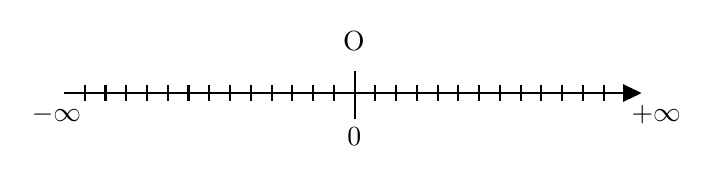
\begin{tikzpicture}[x=0.75pt,y=0.75pt,yscale=-1,xscale=1]
		%uncomment if require: \path (0,771); %set diagram left start at 0, and has height of 771
		
		%Straight Lines [id:da31383788547837055] 
		\draw    (170,124) -- (445.3,124) (180,120) -- (180,128)(190,120) -- (190,128)(200,120) -- (200,128)(210,120) -- (210,128)(220,120) -- (220,128)(230,120) -- (230,128)(240,120) -- (240,128)(250,120) -- (250,128)(260,120) -- (260,128)(270,120) -- (270,128)(280,120) -- (280,128)(290,120) -- (290,128)(300,120) -- (300,128)(310,120) -- (310,128)(320,120) -- (320,128)(330,120) -- (330,128)(340,120) -- (340,128)(350,120) -- (350,128)(360,120) -- (360,128)(370,120) -- (370,128)(380,120) -- (380,128)(390,120) -- (390,128)(400,120) -- (400,128)(410,120) -- (410,128)(420,120) -- (420,128)(430,120) -- (430,128)(440,120) -- (440,128) ;
		\draw [shift={(448.3,124)}, rotate = 180] [fill={rgb, 255:red, 0; green, 0; blue, 0 }  ][line width=0.08]  [draw opacity=0] (8.93,-4.29) -- (0,0) -- (8.93,4.29) -- cycle    ;
		%Straight Lines [id:da8528331730117116] 
		\draw    (310.15,113.5) -- (310.15,136.5) ;
		
		% Text Node
		\draw (442,128.4) node [anchor=north west][inner sep=0.75pt]    {$+\infty $};
		% Text Node
		\draw (153,128.4) node [anchor=north west][inner sep=0.75pt]    {$-\infty $};
		% Text Node
		\draw (303,93) node [anchor=north west][inner sep=0.75pt]   [align=left] {O};
		% Text Node
		\draw (305,139.4) node [anchor=north west][inner sep=0.75pt]    {$0$};
		
		\end{tikzpicture}
		\vspace*{3mm}
		\caption{Typical representation example of an oriented infinite axis with origin}
	\end{figure}
	In most cases we put (traditionally) the axis horizontally and choose the direction from left to right (at least when there is only one axis...).
	\begin{tcolorbox}[title=Remark,arc=10pt,breakable,drop lifted shadow,
  skin=enhanced,
  skin first is subskin of={enhancedfirst}{arc=10pt,no shadow},
  skin middle is subskin of={enhancedmiddle}{arc=10pt,no shadow},
  skin last is subskin of={enhancedlast}{drop lifted shadow}]
	The point (letter) \textbf{O}, frequently represents the number zero in mathematics but we might very well choose to put the origin elsewhere. For example, in physics, the point \textbf{O} is often positioned at the location of the centroid of a system. 
	\end{tcolorbox}
	It is obvious that the fact that the sets of numbers that we discussed in the section Numbers are ordered implies that every number is represented by a single point on this axis. Thus, two distinct real numbers correspond two different points on the axis.

	Thus, there is a correspondence between all numbers and all the points of the axis (in the case of real or complex numbers, it corresponds not a number to each graduation, but a number at each \underline{point} of the axis!). Thus, each number represents a point or a unique graduation and back to each point or graduation is a single number which is the image.

	\pagebreak
	\paragraph{2D representations}\mbox{}\\\\
	There are besides the one dimensional representations, other of higher dimensions (phew!...) like the "\NewTerm{planar representation}\index{planar representation}" that allow us to draw much more than simple points on a one-dimensional straight line but functions of one variable (but also points!). Let's see what this is and looks like:
	\begin{figure}[H]
		\centering
		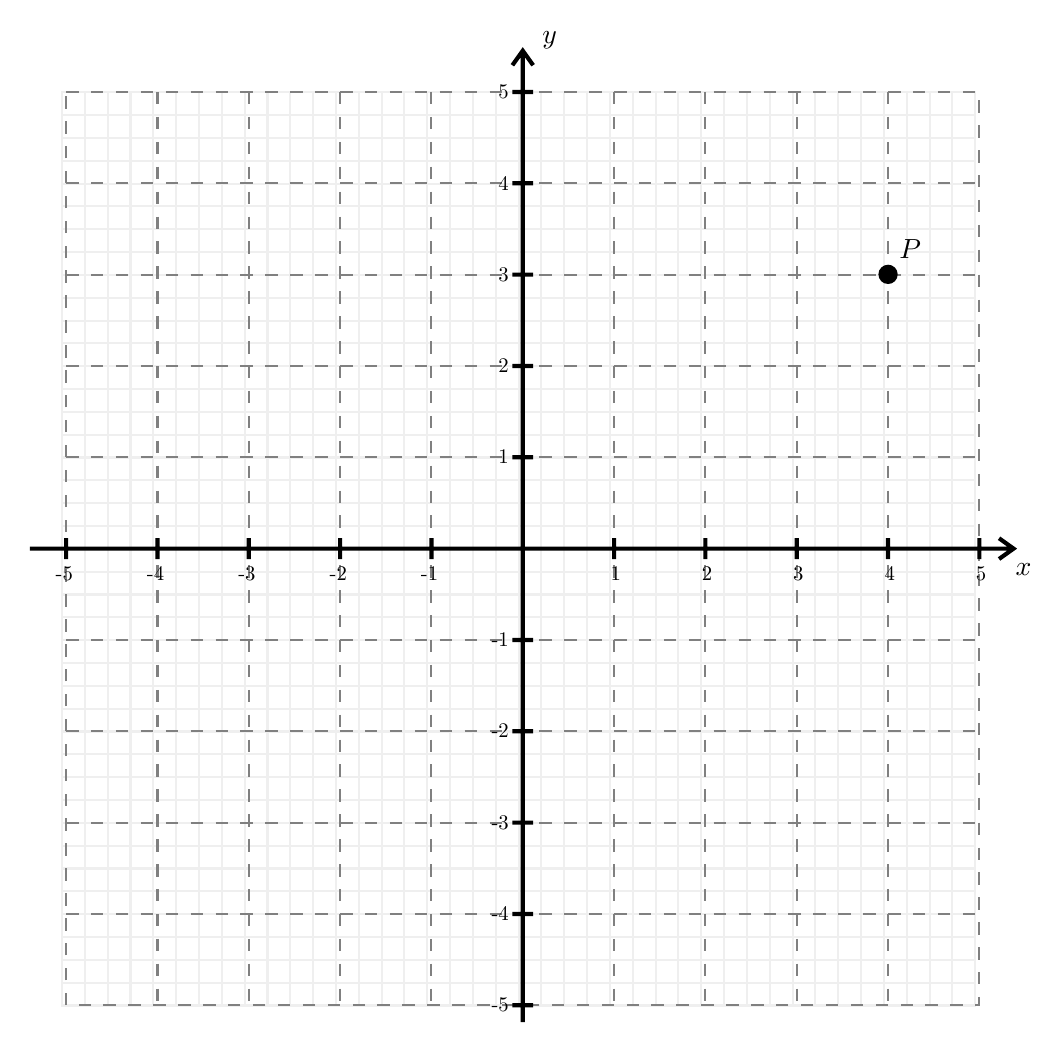
\begin{tikzpicture}[x=0.75pt,y=0.75pt,yscale=-1,xscale=1]
		%uncomment if require: \path (0,1161); %set diagram left start at 0, and has height of 1161
		
		%Shape: Grid [id:dp569692944285175] 
		\draw  [draw opacity=0] (79.86,98.28) -- (519.86,98.28) -- (519.86,538.28) -- (79.86,538.28) -- cycle ; \draw  [color={rgb, 255:red, 239; green, 239; blue, 239 }  ,draw opacity=1 ] (90.86,98.28) -- (90.86,538.28)(101.86,98.28) -- (101.86,538.28)(112.86,98.28) -- (112.86,538.28)(123.86,98.28) -- (123.86,538.28)(134.86,98.28) -- (134.86,538.28)(145.86,98.28) -- (145.86,538.28)(156.86,98.28) -- (156.86,538.28)(167.86,98.28) -- (167.86,538.28)(178.86,98.28) -- (178.86,538.28)(189.86,98.28) -- (189.86,538.28)(200.86,98.28) -- (200.86,538.28)(211.86,98.28) -- (211.86,538.28)(222.86,98.28) -- (222.86,538.28)(233.86,98.28) -- (233.86,538.28)(244.86,98.28) -- (244.86,538.28)(255.86,98.28) -- (255.86,538.28)(266.86,98.28) -- (266.86,538.28)(277.86,98.28) -- (277.86,538.28)(288.86,98.28) -- (288.86,538.28)(299.86,98.28) -- (299.86,538.28)(310.86,98.28) -- (310.86,538.28)(321.86,98.28) -- (321.86,538.28)(332.86,98.28) -- (332.86,538.28)(343.86,98.28) -- (343.86,538.28)(354.86,98.28) -- (354.86,538.28)(365.86,98.28) -- (365.86,538.28)(376.86,98.28) -- (376.86,538.28)(387.86,98.28) -- (387.86,538.28)(398.86,98.28) -- (398.86,538.28)(409.86,98.28) -- (409.86,538.28)(420.86,98.28) -- (420.86,538.28)(431.86,98.28) -- (431.86,538.28)(442.86,98.28) -- (442.86,538.28)(453.86,98.28) -- (453.86,538.28)(464.86,98.28) -- (464.86,538.28)(475.86,98.28) -- (475.86,538.28)(486.86,98.28) -- (486.86,538.28)(497.86,98.28) -- (497.86,538.28)(508.86,98.28) -- (508.86,538.28) ; \draw  [color={rgb, 255:red, 239; green, 239; blue, 239 }  ,draw opacity=1 ] (79.86,109.28) -- (519.86,109.28)(79.86,120.28) -- (519.86,120.28)(79.86,131.28) -- (519.86,131.28)(79.86,142.28) -- (519.86,142.28)(79.86,153.28) -- (519.86,153.28)(79.86,164.28) -- (519.86,164.28)(79.86,175.28) -- (519.86,175.28)(79.86,186.28) -- (519.86,186.28)(79.86,197.28) -- (519.86,197.28)(79.86,208.28) -- (519.86,208.28)(79.86,219.28) -- (519.86,219.28)(79.86,230.28) -- (519.86,230.28)(79.86,241.28) -- (519.86,241.28)(79.86,252.28) -- (519.86,252.28)(79.86,263.28) -- (519.86,263.28)(79.86,274.28) -- (519.86,274.28)(79.86,285.28) -- (519.86,285.28)(79.86,296.28) -- (519.86,296.28)(79.86,307.28) -- (519.86,307.28)(79.86,318.28) -- (519.86,318.28)(79.86,329.28) -- (519.86,329.28)(79.86,340.28) -- (519.86,340.28)(79.86,351.28) -- (519.86,351.28)(79.86,362.28) -- (519.86,362.28)(79.86,373.28) -- (519.86,373.28)(79.86,384.28) -- (519.86,384.28)(79.86,395.28) -- (519.86,395.28)(79.86,406.28) -- (519.86,406.28)(79.86,417.28) -- (519.86,417.28)(79.86,428.28) -- (519.86,428.28)(79.86,439.28) -- (519.86,439.28)(79.86,450.28) -- (519.86,450.28)(79.86,461.28) -- (519.86,461.28)(79.86,472.28) -- (519.86,472.28)(79.86,483.28) -- (519.86,483.28)(79.86,494.28) -- (519.86,494.28)(79.86,505.28) -- (519.86,505.28)(79.86,516.28) -- (519.86,516.28)(79.86,527.28) -- (519.86,527.28) ; \draw  [color={rgb, 255:red, 239; green, 239; blue, 239 }  ,draw opacity=1 ] (79.86,98.28) -- (519.86,98.28) -- (519.86,538.28) -- (79.86,538.28) -- cycle ;
		%Shape: Grid [id:dp8592135899482398] 
		\draw  [draw opacity=0][dash pattern={on 4.5pt off 4.5pt}] (81.86,98.17) -- (521.86,98.17) -- (521.86,538.17) -- (81.86,538.17) -- cycle ; \draw  [color={rgb, 255:red, 128; green, 128; blue, 128 }  ,draw opacity=1 ][dash pattern={on 4.5pt off 4.5pt}] (125.86,98.17) -- (125.86,538.17)(169.86,98.17) -- (169.86,538.17)(213.86,98.17) -- (213.86,538.17)(257.86,98.17) -- (257.86,538.17)(301.86,98.17) -- (301.86,538.17)(345.86,98.17) -- (345.86,538.17)(389.86,98.17) -- (389.86,538.17)(433.86,98.17) -- (433.86,538.17)(477.86,98.17) -- (477.86,538.17) ; \draw  [color={rgb, 255:red, 128; green, 128; blue, 128 }  ,draw opacity=1 ][dash pattern={on 4.5pt off 4.5pt}] (81.86,142.17) -- (521.86,142.17)(81.86,186.17) -- (521.86,186.17)(81.86,230.17) -- (521.86,230.17)(81.86,274.17) -- (521.86,274.17)(81.86,318.17) -- (521.86,318.17)(81.86,362.17) -- (521.86,362.17)(81.86,406.17) -- (521.86,406.17)(81.86,450.17) -- (521.86,450.17)(81.86,494.17) -- (521.86,494.17) ; \draw  [color={rgb, 255:red, 128; green, 128; blue, 128 }  ,draw opacity=1 ][dash pattern={on 4.5pt off 4.5pt}] (81.86,98.17) -- (521.86,98.17) -- (521.86,538.17) -- (81.86,538.17) -- cycle ;
		%Shape: Axis 2D [id:dp6177243705021576] 
		\draw [line width=1.5]  (64.33,318.17) -- (538.33,318.17)(301.86,78.28) -- (301.86,546.28) (531.33,313.17) -- (538.33,318.17) -- (531.33,323.17) (296.86,85.28) -- (301.86,78.28) -- (306.86,85.28) (345.86,313.17) -- (345.86,323.17)(389.86,313.17) -- (389.86,323.17)(433.86,313.17) -- (433.86,323.17)(477.86,313.17) -- (477.86,323.17)(521.86,313.17) -- (521.86,323.17)(257.86,313.17) -- (257.86,323.17)(213.86,313.17) -- (213.86,323.17)(169.86,313.17) -- (169.86,323.17)(125.86,313.17) -- (125.86,323.17)(81.86,313.17) -- (81.86,323.17)(296.86,274.17) -- (306.86,274.17)(296.86,230.17) -- (306.86,230.17)(296.86,186.17) -- (306.86,186.17)(296.86,142.17) -- (306.86,142.17)(296.86,98.17) -- (306.86,98.17)(296.86,362.17) -- (306.86,362.17)(296.86,406.17) -- (306.86,406.17)(296.86,450.17) -- (306.86,450.17)(296.86,494.17) -- (306.86,494.17)(296.86,538.17) -- (306.86,538.17) ;
		\draw   (352.86,330.17) node[anchor=east, scale=0.75]{1} (396.86,330.17) node[anchor=east, scale=0.75]{2} (440.86,330.17) node[anchor=east, scale=0.75]{3} (484.86,330.17) node[anchor=east, scale=0.75]{4} (528.86,330.17) node[anchor=east, scale=0.75]{5} (264.86,330.17) node[anchor=east, scale=0.75]{-1} (220.86,330.17) node[anchor=east, scale=0.75]{-2} (176.86,330.17) node[anchor=east, scale=0.75]{-3} (132.86,330.17) node[anchor=east, scale=0.75]{-4} (88.86,330.17) node[anchor=east, scale=0.75]{-5} (298.86,274.17) node[anchor=east, scale=0.75]{1} (298.86,230.17) node[anchor=east, scale=0.75]{2} (298.86,186.17) node[anchor=east, scale=0.75]{3} (298.86,142.17) node[anchor=east, scale=0.75]{4} (298.86,98.17) node[anchor=east, scale=0.75]{5} (298.86,362.17) node[anchor=east, scale=0.75]{-1} (298.86,406.17) node[anchor=east, scale=0.75]{-2} (298.86,450.17) node[anchor=east, scale=0.75]{-3} (298.86,494.17) node[anchor=east, scale=0.75]{-4} (298.86,538.17) node[anchor=east, scale=0.75]{-5} ;
		%Shape: Circle [id:dp3585791740414457] 
\draw  [fill={rgb, 255:red, 0; green, 0; blue, 0 }  ,fill opacity=1 ] (473.72,186.03) .. controls (473.72,183.74) and (475.58,181.89) .. (477.86,181.89) .. controls (480.15,181.89) and (482,183.74) .. (482,186.03) .. controls (482,188.32) and (480.15,190.17) .. (477.86,190.17) .. controls (475.58,190.17) and (473.72,188.32) .. (473.72,186.03) -- cycle ;
		
		% Text Node
		\draw (309.86,67.68) node [anchor=north west][inner sep=0.75pt]    {$y$};
		% Text Node
		\draw (537.86,323.68) node [anchor=north west][inner sep=0.75pt]    {$x$};
		% Text Node
		\draw (481.86,167.68) node [anchor=north west][inner sep=0.75pt]    {$P$};
		\end{tikzpicture}
		\vspace*{3mm}
		\caption{Position of a point in a cartesian plane}
	\end{figure}
	In the above figure we have added two graduation that helps us to identify uniquely the position of the point $P$ given by $P(x,y)=P(+4,+3)=P(4,3)$. We then speak of "cartesian coordinates of a point".

	In single-variable calculus, the functions that one encounters are functions of a variable (usually $x$ or $t$) that varies over some subset of the real number line (which we denote by $\mathbb{R}$). For such a function, say, $y = f (x)$, the graph of the function $f$ consists of the points:
	
	These points lie in the Euclidean plane, which, in the Cartesian or rectangular
coordinate system, consists of all ordered pairs of real numbers $(a,b)$. We use the word "Euclidean" to denote a system in which all the usual rules of Euclidean geometry hold (\SeeChapter{see section Euclidean Geometry page \pageref{hilbert axioms}}). We denote the Euclidean plane by $\mathbb{R}^2$ where the exponent "$2$" represents the number of dimensions of the plane.

	Thus we can for each of a variable $x$ on a horizontal axis, named commonly "\NewTerm{$x$-axis\index{$x$-axis}}" match a value $y$ through a function $f$ such that:
	
	plotted on a vertical axis, named commonly the "\NewTerm{$y$-axis}\index{$y$-axis}" which passes through the junction defined by the origin $\text{O}$ such tat (arbitrary example):
	\begin{figure}[H]
		\centering
		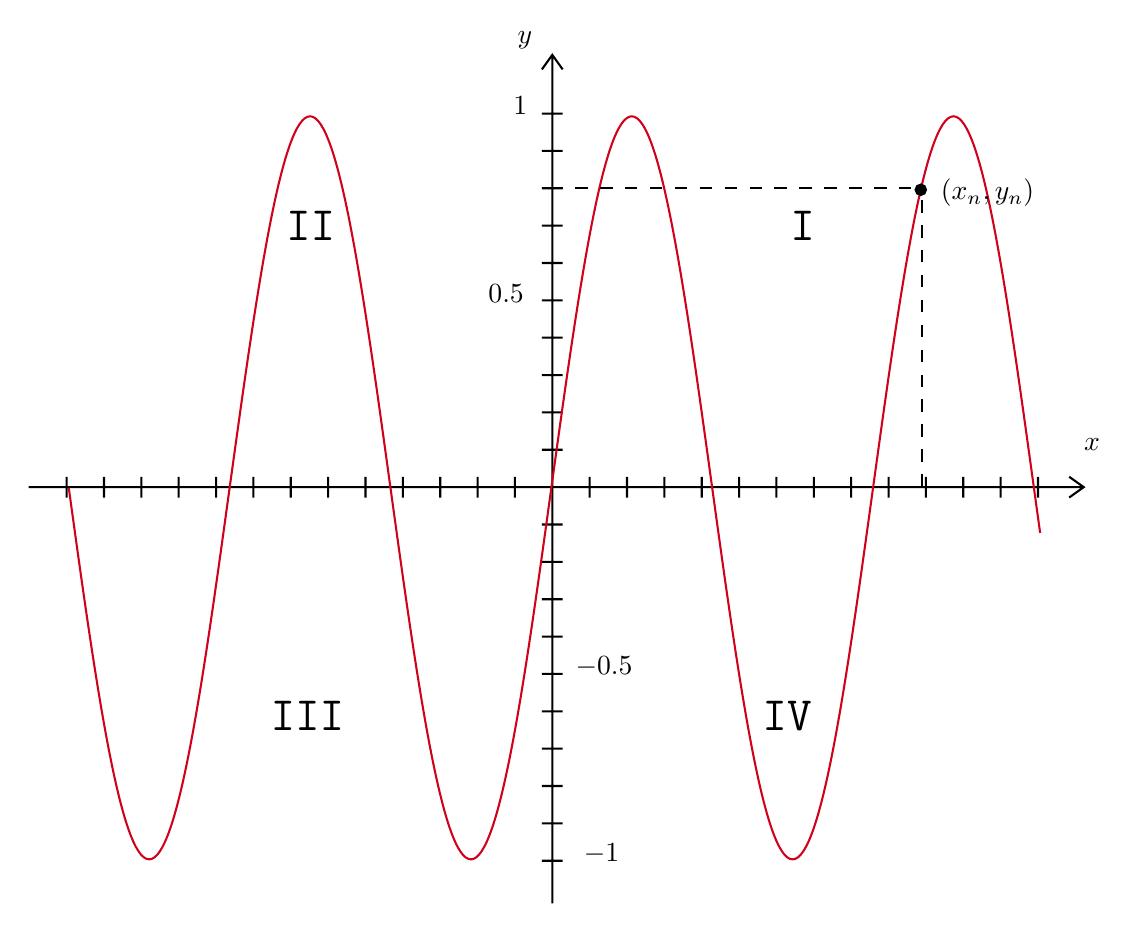
\begin{tikzpicture}[x=0.75pt,y=0.75pt,yscale=-1,xscale=1]
		%uncomment if require: \path (0,670); %set diagram left start at 0, and has height of 670
		
		%Shape: Axis 2D [id:dp21503549174714842] 
		\draw  (68,241.27) -- (576.3,241.27)(320.26,33) -- (320.26,441.8) (569.3,236.27) -- (576.3,241.27) -- (569.3,246.27) (315.26,40) -- (320.26,33) -- (325.26,40) (338.26,236.27) -- (338.26,246.27)(356.26,236.27) -- (356.26,246.27)(374.26,236.27) -- (374.26,246.27)(392.26,236.27) -- (392.26,246.27)(410.26,236.27) -- (410.26,246.27)(428.26,236.27) -- (428.26,246.27)(446.26,236.27) -- (446.26,246.27)(464.26,236.27) -- (464.26,246.27)(482.26,236.27) -- (482.26,246.27)(500.26,236.27) -- (500.26,246.27)(518.26,236.27) -- (518.26,246.27)(536.26,236.27) -- (536.26,246.27)(554.26,236.27) -- (554.26,246.27)(302.26,236.27) -- (302.26,246.27)(284.26,236.27) -- (284.26,246.27)(266.26,236.27) -- (266.26,246.27)(248.26,236.27) -- (248.26,246.27)(230.26,236.27) -- (230.26,246.27)(212.26,236.27) -- (212.26,246.27)(194.26,236.27) -- (194.26,246.27)(176.26,236.27) -- (176.26,246.27)(158.26,236.27) -- (158.26,246.27)(140.26,236.27) -- (140.26,246.27)(122.26,236.27) -- (122.26,246.27)(104.26,236.27) -- (104.26,246.27)(86.26,236.27) -- (86.26,246.27)(315.26,223.27) -- (325.26,223.27)(315.26,205.27) -- (325.26,205.27)(315.26,187.27) -- (325.26,187.27)(315.26,169.27) -- (325.26,169.27)(315.26,151.27) -- (325.26,151.27)(315.26,133.27) -- (325.26,133.27)(315.26,115.27) -- (325.26,115.27)(315.26,97.27) -- (325.26,97.27)(315.26,79.27) -- (325.26,79.27)(315.26,61.27) -- (325.26,61.27)(315.26,259.27) -- (325.26,259.27)(315.26,277.27) -- (325.26,277.27)(315.26,295.27) -- (325.26,295.27)(315.26,313.27) -- (325.26,313.27)(315.26,331.27) -- (325.26,331.27)(315.26,349.27) -- (325.26,349.27)(315.26,367.27) -- (325.26,367.27)(315.26,385.27) -- (325.26,385.27)(315.26,403.27) -- (325.26,403.27)(315.26,421.27) -- (325.26,421.27) ;
		\draw   ;
		%Shape: Wave [id:dp3533280072317033] 
		\draw  [color={rgb, 255:red, 208; green, 2; blue, 27 }  ,draw opacity=1 ] (87.3,241.6) .. controls (99.94,333.3) and (112.03,420.6) .. (126.05,420.6) .. controls (140.07,420.6) and (152.16,333.3) .. (164.8,241.6) .. controls (177.44,149.9) and (189.53,62.6) .. (203.55,62.6) .. controls (217.57,62.6) and (229.66,149.9) .. (242.3,241.6) .. controls (254.94,333.3) and (267.03,420.6) .. (281.05,420.6) .. controls (295.07,420.6) and (307.16,333.3) .. (319.8,241.6) .. controls (332.44,149.9) and (344.53,62.6) .. (358.55,62.6) .. controls (372.57,62.6) and (384.66,149.9) .. (397.3,241.6) .. controls (409.94,333.3) and (422.03,420.6) .. (436.05,420.6) .. controls (450.07,420.6) and (462.16,333.3) .. (474.8,241.6) .. controls (487.44,149.9) and (499.53,62.6) .. (513.55,62.6) .. controls (527.57,62.6) and (539.66,149.9) .. (552.3,241.6) .. controls (553.3,248.88) and (554.3,256.13) .. (555.3,263.31) ;
		%Straight Lines [id:da7430234065805821] 
		\draw  [dash pattern={on 4.5pt off 4.5pt}]  (319.3,97) -- (498.3,97) ;
		%Straight Lines [id:da4455333738888003] 
		\draw  [dash pattern={on 4.5pt off 4.5pt}]  (498.3,241) -- (498.3,97) ;
		%Shape: Circle [id:dp37776284466742704] 
		\draw  [fill={rgb, 255:red, 0; green, 0; blue, 0 }  ,fill opacity=1 ] (495.3,98) .. controls (495.3,96.62) and (496.42,95.5) .. (497.8,95.5) .. controls (499.18,95.5) and (500.3,96.62) .. (500.3,98) .. controls (500.3,99.38) and (499.18,100.5) .. (497.8,100.5) .. controls (496.42,100.5) and (495.3,99.38) .. (495.3,98) -- cycle ;
		
		% Text Node
		\draw (302,20.4) node [anchor=north west][inner sep=0.75pt]    {$y$};
		% Text Node
		\draw (575,216.4) node [anchor=north west][inner sep=0.75pt]    {$x$};
		% Text Node
		\draw (300,51.4) node [anchor=north west][inner sep=0.75pt]    {$1$};
		% Text Node
		\draw (288,142.4) node [anchor=north west][inner sep=0.75pt]    {$0.5$};
		% Text Node
		\draw (330,321.4) node [anchor=north west][inner sep=0.75pt]    {$-0.5$};
		% Text Node
		\draw (334,411.4) node [anchor=north west][inner sep=0.75pt]    {$-1$};
		% Text Node
		\draw (433.5,106.9) node [anchor=north west][inner sep=0.75pt]  [font=\LARGE]  {$\texttt{I}$};
		% Text Node
		\draw (190.5,106.9) node [anchor=north west][inner sep=0.75pt]  [font=\LARGE]  {$\texttt{II}$};
		% Text Node
		\draw (183,342.9) node [anchor=north west][inner sep=0.75pt]  [font=\LARGE]  {$\texttt{III}$};
		% Text Node
		\draw (420,342.9) node [anchor=north west][inner sep=0.75pt]  [font=\LARGE]  {$\texttt{IV}$};
		% Text Node
		\draw (506,91.4) node [anchor=north west][inner sep=0.75pt]    {$( x_{n} ,y_{n})$};
		\end{tikzpicture}
		\vspace*{3mm}
		\caption[]{Typical example of a planar representation with orthogonal axes, origin O and the $4$ quadrants}
	\end{figure}
	All points of the plane (that latter being denoted with the variations $X\text{O}Y$, $XY$ or $x\text{O}y$, $\text{O}xy$, $xy$) have for "\NewTerm{abscissa}\index{abscissa}" traditionally the $x$-values corresponding to the independent variable (horizontal axes by tradition) of the function and for "\NewTerm{ordinate}\index{ordinate}" the corresponding value of the function (vertical axes by tradition). All these generated what is named the "\NewTerm{planar graph}\index{planar graph}" of the function. If there is no confusion, we just say "\NewTerm{graph}\index{graph}".
	\begin{figure}[H]
		\centering
		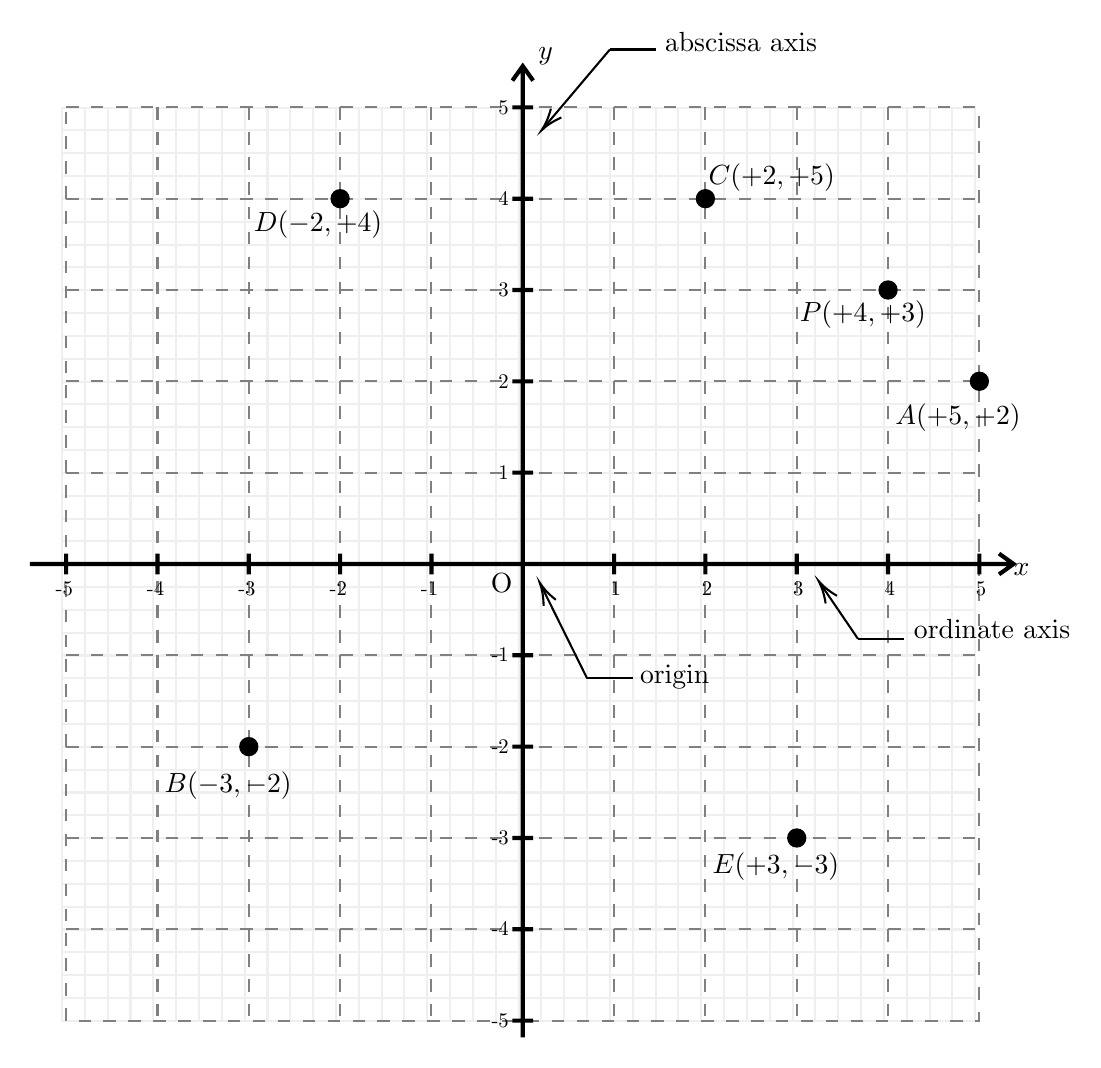
\begin{tikzpicture}[x=0.75pt,y=0.75pt,yscale=-1,xscale=1]
		%uncomment if require: \path (0,1161); %set diagram left start at 0, and has height of 1161
		
		%Shape: Grid [id:dp569692944285175] 
		\draw  [draw opacity=0] (79.86,98.28) -- (519.86,98.28) -- (519.86,538.28) -- (79.86,538.28) -- cycle ; \draw  [color={rgb, 255:red, 239; green, 239; blue, 239 }  ,draw opacity=1 ] (90.86,98.28) -- (90.86,538.28)(101.86,98.28) -- (101.86,538.28)(112.86,98.28) -- (112.86,538.28)(123.86,98.28) -- (123.86,538.28)(134.86,98.28) -- (134.86,538.28)(145.86,98.28) -- (145.86,538.28)(156.86,98.28) -- (156.86,538.28)(167.86,98.28) -- (167.86,538.28)(178.86,98.28) -- (178.86,538.28)(189.86,98.28) -- (189.86,538.28)(200.86,98.28) -- (200.86,538.28)(211.86,98.28) -- (211.86,538.28)(222.86,98.28) -- (222.86,538.28)(233.86,98.28) -- (233.86,538.28)(244.86,98.28) -- (244.86,538.28)(255.86,98.28) -- (255.86,538.28)(266.86,98.28) -- (266.86,538.28)(277.86,98.28) -- (277.86,538.28)(288.86,98.28) -- (288.86,538.28)(299.86,98.28) -- (299.86,538.28)(310.86,98.28) -- (310.86,538.28)(321.86,98.28) -- (321.86,538.28)(332.86,98.28) -- (332.86,538.28)(343.86,98.28) -- (343.86,538.28)(354.86,98.28) -- (354.86,538.28)(365.86,98.28) -- (365.86,538.28)(376.86,98.28) -- (376.86,538.28)(387.86,98.28) -- (387.86,538.28)(398.86,98.28) -- (398.86,538.28)(409.86,98.28) -- (409.86,538.28)(420.86,98.28) -- (420.86,538.28)(431.86,98.28) -- (431.86,538.28)(442.86,98.28) -- (442.86,538.28)(453.86,98.28) -- (453.86,538.28)(464.86,98.28) -- (464.86,538.28)(475.86,98.28) -- (475.86,538.28)(486.86,98.28) -- (486.86,538.28)(497.86,98.28) -- (497.86,538.28)(508.86,98.28) -- (508.86,538.28) ; \draw  [color={rgb, 255:red, 239; green, 239; blue, 239 }  ,draw opacity=1 ] (79.86,109.28) -- (519.86,109.28)(79.86,120.28) -- (519.86,120.28)(79.86,131.28) -- (519.86,131.28)(79.86,142.28) -- (519.86,142.28)(79.86,153.28) -- (519.86,153.28)(79.86,164.28) -- (519.86,164.28)(79.86,175.28) -- (519.86,175.28)(79.86,186.28) -- (519.86,186.28)(79.86,197.28) -- (519.86,197.28)(79.86,208.28) -- (519.86,208.28)(79.86,219.28) -- (519.86,219.28)(79.86,230.28) -- (519.86,230.28)(79.86,241.28) -- (519.86,241.28)(79.86,252.28) -- (519.86,252.28)(79.86,263.28) -- (519.86,263.28)(79.86,274.28) -- (519.86,274.28)(79.86,285.28) -- (519.86,285.28)(79.86,296.28) -- (519.86,296.28)(79.86,307.28) -- (519.86,307.28)(79.86,318.28) -- (519.86,318.28)(79.86,329.28) -- (519.86,329.28)(79.86,340.28) -- (519.86,340.28)(79.86,351.28) -- (519.86,351.28)(79.86,362.28) -- (519.86,362.28)(79.86,373.28) -- (519.86,373.28)(79.86,384.28) -- (519.86,384.28)(79.86,395.28) -- (519.86,395.28)(79.86,406.28) -- (519.86,406.28)(79.86,417.28) -- (519.86,417.28)(79.86,428.28) -- (519.86,428.28)(79.86,439.28) -- (519.86,439.28)(79.86,450.28) -- (519.86,450.28)(79.86,461.28) -- (519.86,461.28)(79.86,472.28) -- (519.86,472.28)(79.86,483.28) -- (519.86,483.28)(79.86,494.28) -- (519.86,494.28)(79.86,505.28) -- (519.86,505.28)(79.86,516.28) -- (519.86,516.28)(79.86,527.28) -- (519.86,527.28) ; \draw  [color={rgb, 255:red, 239; green, 239; blue, 239 }  ,draw opacity=1 ] (79.86,98.28) -- (519.86,98.28) -- (519.86,538.28) -- (79.86,538.28) -- cycle ;
		%Shape: Grid [id:dp8592135899482398] 
		\draw  [draw opacity=0][dash pattern={on 4.5pt off 4.5pt}] (81.86,98.17) -- (521.86,98.17) -- (521.86,538.17) -- (81.86,538.17) -- cycle ; \draw  [color={rgb, 255:red, 128; green, 128; blue, 128 }  ,draw opacity=1 ][dash pattern={on 4.5pt off 4.5pt}] (125.86,98.17) -- (125.86,538.17)(169.86,98.17) -- (169.86,538.17)(213.86,98.17) -- (213.86,538.17)(257.86,98.17) -- (257.86,538.17)(301.86,98.17) -- (301.86,538.17)(345.86,98.17) -- (345.86,538.17)(389.86,98.17) -- (389.86,538.17)(433.86,98.17) -- (433.86,538.17)(477.86,98.17) -- (477.86,538.17) ; \draw  [color={rgb, 255:red, 128; green, 128; blue, 128 }  ,draw opacity=1 ][dash pattern={on 4.5pt off 4.5pt}] (81.86,142.17) -- (521.86,142.17)(81.86,186.17) -- (521.86,186.17)(81.86,230.17) -- (521.86,230.17)(81.86,274.17) -- (521.86,274.17)(81.86,318.17) -- (521.86,318.17)(81.86,362.17) -- (521.86,362.17)(81.86,406.17) -- (521.86,406.17)(81.86,450.17) -- (521.86,450.17)(81.86,494.17) -- (521.86,494.17) ; \draw  [color={rgb, 255:red, 128; green, 128; blue, 128 }  ,draw opacity=1 ][dash pattern={on 4.5pt off 4.5pt}] (81.86,98.17) -- (521.86,98.17) -- (521.86,538.17) -- (81.86,538.17) -- cycle ;
		%Shape: Axis 2D [id:dp6177243705021576] 
		\draw [line width=1.5]  (64.33,318.17) -- (538.33,318.17)(301.86,78.28) -- (301.86,546.28) (531.33,313.17) -- (538.33,318.17) -- (531.33,323.17) (296.86,85.28) -- (301.86,78.28) -- (306.86,85.28) (345.86,313.17) -- (345.86,323.17)(389.86,313.17) -- (389.86,323.17)(433.86,313.17) -- (433.86,323.17)(477.86,313.17) -- (477.86,323.17)(521.86,313.17) -- (521.86,323.17)(257.86,313.17) -- (257.86,323.17)(213.86,313.17) -- (213.86,323.17)(169.86,313.17) -- (169.86,323.17)(125.86,313.17) -- (125.86,323.17)(81.86,313.17) -- (81.86,323.17)(296.86,274.17) -- (306.86,274.17)(296.86,230.17) -- (306.86,230.17)(296.86,186.17) -- (306.86,186.17)(296.86,142.17) -- (306.86,142.17)(296.86,98.17) -- (306.86,98.17)(296.86,362.17) -- (306.86,362.17)(296.86,406.17) -- (306.86,406.17)(296.86,450.17) -- (306.86,450.17)(296.86,494.17) -- (306.86,494.17)(296.86,538.17) -- (306.86,538.17) ;
		\draw   (352.86,330.17) node[anchor=east, scale=0.75]{1} (396.86,330.17) node[anchor=east, scale=0.75]{2} (440.86,330.17) node[anchor=east, scale=0.75]{3} (484.86,330.17) node[anchor=east, scale=0.75]{4} (528.86,330.17) node[anchor=east, scale=0.75]{5} (264.86,330.17) node[anchor=east, scale=0.75]{-1} (220.86,330.17) node[anchor=east, scale=0.75]{-2} (176.86,330.17) node[anchor=east, scale=0.75]{-3} (132.86,330.17) node[anchor=east, scale=0.75]{-4} (88.86,330.17) node[anchor=east, scale=0.75]{-5} (298.86,274.17) node[anchor=east, scale=0.75]{1} (298.86,230.17) node[anchor=east, scale=0.75]{2} (298.86,186.17) node[anchor=east, scale=0.75]{3} (298.86,142.17) node[anchor=east, scale=0.75]{4} (298.86,98.17) node[anchor=east, scale=0.75]{5} (298.86,362.17) node[anchor=east, scale=0.75]{-1} (298.86,406.17) node[anchor=east, scale=0.75]{-2} (298.86,450.17) node[anchor=east, scale=0.75]{-3} (298.86,494.17) node[anchor=east, scale=0.75]{-4} (298.86,538.17) node[anchor=east, scale=0.75]{-5} ;
		%Shape: Circle [id:dp3585791740414457] 
		\draw  [fill={rgb, 255:red, 0; green, 0; blue, 0 }  ,fill opacity=1 ] (385.72,142.17) .. controls (385.72,139.88) and (387.58,138.03) .. (389.86,138.03) .. controls (392.15,138.03) and (394,139.88) .. (394,142.17) .. controls (394,144.46) and (392.15,146.31) .. (389.86,146.31) .. controls (387.58,146.31) and (385.72,144.46) .. (385.72,142.17) -- cycle ;
		%Shape: Circle [id:dp4340792580097408] 
		\draw  [fill={rgb, 255:red, 0; green, 0; blue, 0 }  ,fill opacity=1 ] (473.72,186.17) .. controls (473.72,183.88) and (475.58,182.03) .. (477.86,182.03) .. controls (480.15,182.03) and (482,183.88) .. (482,186.17) .. controls (482,188.46) and (480.15,190.31) .. (477.86,190.31) .. controls (475.58,190.31) and (473.72,188.46) .. (473.72,186.17) -- cycle ;
		%Shape: Circle [id:dp9347016722228567] 
		\draw  [fill={rgb, 255:red, 0; green, 0; blue, 0 }  ,fill opacity=1 ] (517.72,230.14) .. controls (517.72,227.85) and (519.58,226) .. (521.86,226) .. controls (524.15,226) and (526,227.85) .. (526,230.14) .. controls (526,232.43) and (524.15,234.28) .. (521.86,234.28) .. controls (519.58,234.28) and (517.72,232.43) .. (517.72,230.14) -- cycle ;
		%Shape: Circle [id:dp13285311159548185] 
		\draw  [fill={rgb, 255:red, 0; green, 0; blue, 0 }  ,fill opacity=1 ] (209.72,142.17) .. controls (209.72,139.88) and (211.58,138.03) .. (213.86,138.03) .. controls (216.15,138.03) and (218,139.88) .. (218,142.17) .. controls (218,144.46) and (216.15,146.31) .. (213.86,146.31) .. controls (211.58,146.31) and (209.72,144.46) .. (209.72,142.17) -- cycle ;
		%Shape: Circle [id:dp48043860085523504] 
		\draw  [fill={rgb, 255:red, 0; green, 0; blue, 0 }  ,fill opacity=1 ] (165.72,406.17) .. controls (165.72,403.88) and (167.58,402.03) .. (169.86,402.03) .. controls (172.15,402.03) and (174,403.88) .. (174,406.17) .. controls (174,408.46) and (172.15,410.31) .. (169.86,410.31) .. controls (167.58,410.31) and (165.72,408.46) .. (165.72,406.17) -- cycle ;
		%Shape: Circle [id:dp956327891028663] 
		\draw  [fill={rgb, 255:red, 0; green, 0; blue, 0 }  ,fill opacity=1 ] (429.72,450.17) .. controls (429.72,447.88) and (431.58,446.03) .. (433.86,446.03) .. controls (436.15,446.03) and (438,447.88) .. (438,450.17) .. controls (438,452.46) and (436.15,454.31) .. (433.86,454.31) .. controls (431.58,454.31) and (429.72,452.46) .. (429.72,450.17) -- cycle ;
		%Straight Lines [id:da7677125479209048] 
		\draw    (332.86,373.28) -- (310.89,328.89) ;
		\draw [shift={(310,327.1)}, rotate = 63.66] [color={rgb, 255:red, 0; green, 0; blue, 0 }  ][line width=0.75]    (10.93,-3.29) .. controls (6.95,-1.4) and (3.31,-0.3) .. (0,0) .. controls (3.31,0.3) and (6.95,1.4) .. (10.93,3.29)   ;
		%Straight Lines [id:da127805876141579] 
		\draw    (332.86,373.28) -- (354.86,373.28) ;
		%Straight Lines [id:da4290888085536009] 
		\draw    (343.86,70.28) -- (312.16,107.75) ;
		\draw [shift={(310.86,109.28)}, rotate = 310.24] [color={rgb, 255:red, 0; green, 0; blue, 0 }  ][line width=0.75]    (10.93,-3.29) .. controls (6.95,-1.4) and (3.31,-0.3) .. (0,0) .. controls (3.31,0.3) and (6.95,1.4) .. (10.93,3.29)   ;
		%Straight Lines [id:da65066068911189] 
		\draw    (343.86,70.28) -- (365.86,70.28) ;
		%Straight Lines [id:da9753824973296665] 
		\draw    (463.36,354.23) -- (445.49,327.98) ;
		\draw [shift={(444.36,326.32)}, rotate = 55.75] [color={rgb, 255:red, 0; green, 0; blue, 0 }  ][line width=0.75]    (10.93,-3.29) .. controls (6.95,-1.4) and (3.31,-0.3) .. (0,0) .. controls (3.31,0.3) and (6.95,1.4) .. (10.93,3.29)   ;
		%Straight Lines [id:da28270488568990215] 
		\draw    (463.36,354.23) -- (485.36,354.23) ;
		
		% Text Node
		\draw (307.86,67.68) node [anchor=north west][inner sep=0.75pt]    {$y$};
		% Text Node
		\draw (536.86,316.68) node [anchor=north west][inner sep=0.75pt]    {$x$};
		% Text Node
		\draw (389.86,123.68) node [anchor=north west][inner sep=0.75pt]    {$C( +2,+5)$};
		% Text Node
		\draw (433.86,189.68) node [anchor=north west][inner sep=0.75pt]    {$P( +4,+3)$};
		% Text Node
		\draw (479.86,239.68) node [anchor=north west][inner sep=0.75pt]    {$A( +5,+2)$};
		% Text Node
		\draw (170.86,146.57) node [anchor=north west][inner sep=0.75pt]    {$D( -2,+4)$};
		% Text Node
		\draw (127.86,416.68) node [anchor=north west][inner sep=0.75pt]    {$B( -3,-2)$};
		% Text Node
		\draw (391.86,455.68) node [anchor=north west][inner sep=0.75pt]    {$E( +3,-3)$};
		% Text Node
		\draw (285,321.1) node [anchor=north west][inner sep=0.75pt]   [align=left] {O};
		% Text Node
		\draw (356.86,365.28) node [anchor=north west][inner sep=0.75pt]   [align=left] {origin};
		% Text Node
		\draw (368.86,60.28) node [anchor=north west][inner sep=0.75pt]   [align=left] {abscissa axis};
		% Text Node
		\draw (488.86,343.28) node [anchor=north west][inner sep=0.75pt]   [align=left] {ordinate axis};
		\end{tikzpicture}
		\vspace*{3mm}
		\caption{Vocabulary planar graph}
	\end{figure}
	An interesting detailed example for middle schools students that may help is the planar representation of the following line equation:
	
	That gives in the range $x\in [-3.3,+3.3]$ the following graph:
	\begin{figure}[H]
		\centering
		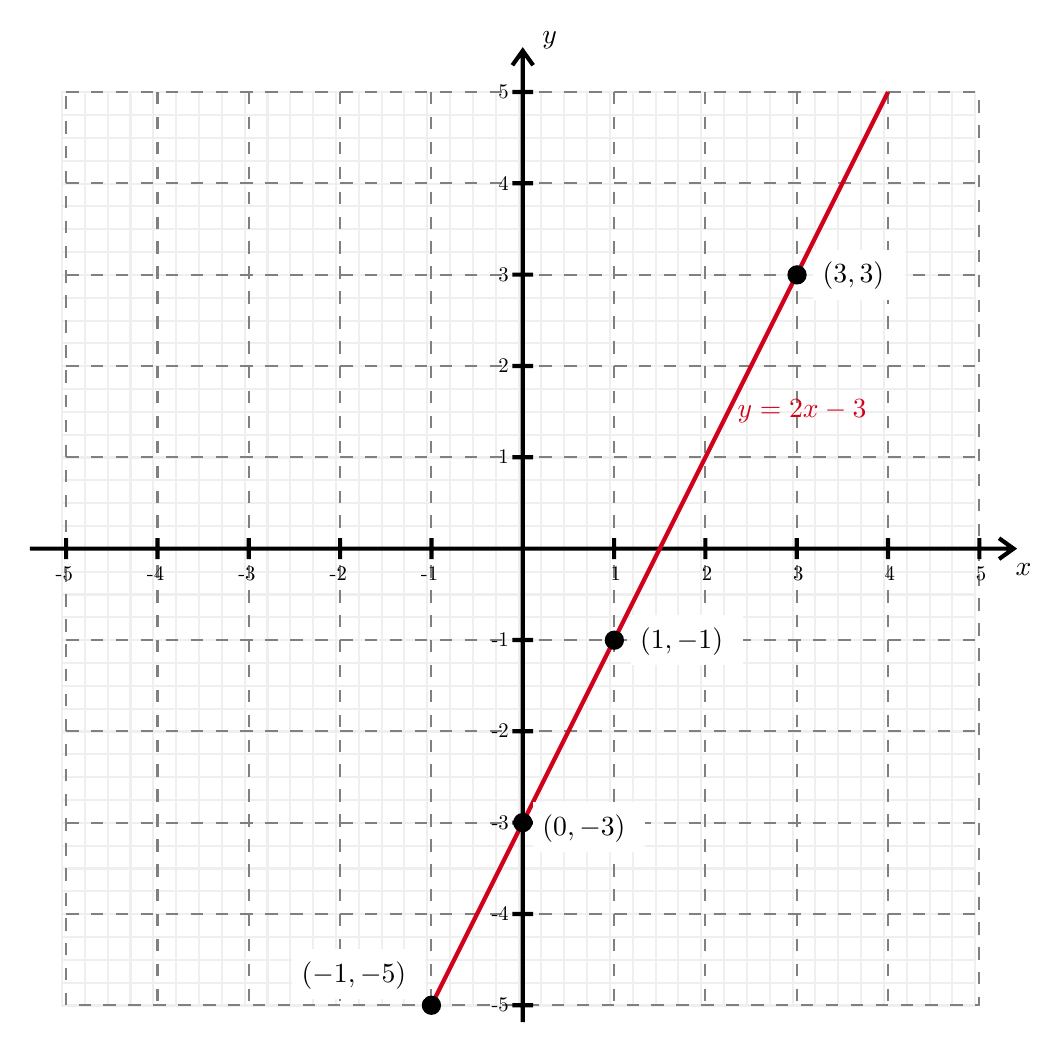
\begin{tikzpicture}[x=0.75pt,y=0.75pt,yscale=-1,xscale=1]
		%uncomment if require: \path (0,1161); %set diagram left start at 0, and has height of 1161
		
		%Shape: Grid [id:dp569692944285175] 
		\draw  [draw opacity=0] (79.86,98.28) -- (519.86,98.28) -- (519.86,538.28) -- (79.86,538.28) -- cycle ; \draw  [color={rgb, 255:red, 239; green, 239; blue, 239 }  ,draw opacity=1 ] (90.86,98.28) -- (90.86,538.28)(101.86,98.28) -- (101.86,538.28)(112.86,98.28) -- (112.86,538.28)(123.86,98.28) -- (123.86,538.28)(134.86,98.28) -- (134.86,538.28)(145.86,98.28) -- (145.86,538.28)(156.86,98.28) -- (156.86,538.28)(167.86,98.28) -- (167.86,538.28)(178.86,98.28) -- (178.86,538.28)(189.86,98.28) -- (189.86,538.28)(200.86,98.28) -- (200.86,538.28)(211.86,98.28) -- (211.86,538.28)(222.86,98.28) -- (222.86,538.28)(233.86,98.28) -- (233.86,538.28)(244.86,98.28) -- (244.86,538.28)(255.86,98.28) -- (255.86,538.28)(266.86,98.28) -- (266.86,538.28)(277.86,98.28) -- (277.86,538.28)(288.86,98.28) -- (288.86,538.28)(299.86,98.28) -- (299.86,538.28)(310.86,98.28) -- (310.86,538.28)(321.86,98.28) -- (321.86,538.28)(332.86,98.28) -- (332.86,538.28)(343.86,98.28) -- (343.86,538.28)(354.86,98.28) -- (354.86,538.28)(365.86,98.28) -- (365.86,538.28)(376.86,98.28) -- (376.86,538.28)(387.86,98.28) -- (387.86,538.28)(398.86,98.28) -- (398.86,538.28)(409.86,98.28) -- (409.86,538.28)(420.86,98.28) -- (420.86,538.28)(431.86,98.28) -- (431.86,538.28)(442.86,98.28) -- (442.86,538.28)(453.86,98.28) -- (453.86,538.28)(464.86,98.28) -- (464.86,538.28)(475.86,98.28) -- (475.86,538.28)(486.86,98.28) -- (486.86,538.28)(497.86,98.28) -- (497.86,538.28)(508.86,98.28) -- (508.86,538.28) ; \draw  [color={rgb, 255:red, 239; green, 239; blue, 239 }  ,draw opacity=1 ] (79.86,109.28) -- (519.86,109.28)(79.86,120.28) -- (519.86,120.28)(79.86,131.28) -- (519.86,131.28)(79.86,142.28) -- (519.86,142.28)(79.86,153.28) -- (519.86,153.28)(79.86,164.28) -- (519.86,164.28)(79.86,175.28) -- (519.86,175.28)(79.86,186.28) -- (519.86,186.28)(79.86,197.28) -- (519.86,197.28)(79.86,208.28) -- (519.86,208.28)(79.86,219.28) -- (519.86,219.28)(79.86,230.28) -- (519.86,230.28)(79.86,241.28) -- (519.86,241.28)(79.86,252.28) -- (519.86,252.28)(79.86,263.28) -- (519.86,263.28)(79.86,274.28) -- (519.86,274.28)(79.86,285.28) -- (519.86,285.28)(79.86,296.28) -- (519.86,296.28)(79.86,307.28) -- (519.86,307.28)(79.86,318.28) -- (519.86,318.28)(79.86,329.28) -- (519.86,329.28)(79.86,340.28) -- (519.86,340.28)(79.86,351.28) -- (519.86,351.28)(79.86,362.28) -- (519.86,362.28)(79.86,373.28) -- (519.86,373.28)(79.86,384.28) -- (519.86,384.28)(79.86,395.28) -- (519.86,395.28)(79.86,406.28) -- (519.86,406.28)(79.86,417.28) -- (519.86,417.28)(79.86,428.28) -- (519.86,428.28)(79.86,439.28) -- (519.86,439.28)(79.86,450.28) -- (519.86,450.28)(79.86,461.28) -- (519.86,461.28)(79.86,472.28) -- (519.86,472.28)(79.86,483.28) -- (519.86,483.28)(79.86,494.28) -- (519.86,494.28)(79.86,505.28) -- (519.86,505.28)(79.86,516.28) -- (519.86,516.28)(79.86,527.28) -- (519.86,527.28) ; \draw  [color={rgb, 255:red, 239; green, 239; blue, 239 }  ,draw opacity=1 ] (79.86,98.28) -- (519.86,98.28) -- (519.86,538.28) -- (79.86,538.28) -- cycle ;
		%Shape: Grid [id:dp8592135899482398] 
		\draw  [draw opacity=0][dash pattern={on 4.5pt off 4.5pt}] (81.86,98.17) -- (521.86,98.17) -- (521.86,538.17) -- (81.86,538.17) -- cycle ; \draw  [color={rgb, 255:red, 128; green, 128; blue, 128 }  ,draw opacity=1 ][dash pattern={on 4.5pt off 4.5pt}] (125.86,98.17) -- (125.86,538.17)(169.86,98.17) -- (169.86,538.17)(213.86,98.17) -- (213.86,538.17)(257.86,98.17) -- (257.86,538.17)(301.86,98.17) -- (301.86,538.17)(345.86,98.17) -- (345.86,538.17)(389.86,98.17) -- (389.86,538.17)(433.86,98.17) -- (433.86,538.17)(477.86,98.17) -- (477.86,538.17) ; \draw  [color={rgb, 255:red, 128; green, 128; blue, 128 }  ,draw opacity=1 ][dash pattern={on 4.5pt off 4.5pt}] (81.86,142.17) -- (521.86,142.17)(81.86,186.17) -- (521.86,186.17)(81.86,230.17) -- (521.86,230.17)(81.86,274.17) -- (521.86,274.17)(81.86,318.17) -- (521.86,318.17)(81.86,362.17) -- (521.86,362.17)(81.86,406.17) -- (521.86,406.17)(81.86,450.17) -- (521.86,450.17)(81.86,494.17) -- (521.86,494.17) ; \draw  [color={rgb, 255:red, 128; green, 128; blue, 128 }  ,draw opacity=1 ][dash pattern={on 4.5pt off 4.5pt}] (81.86,98.17) -- (521.86,98.17) -- (521.86,538.17) -- (81.86,538.17) -- cycle ;
		%Shape: Axis 2D [id:dp6177243705021576] 
		\draw [line width=1.5]  (64.33,318.17) -- (538.33,318.17)(301.86,78.28) -- (301.86,546.28) (531.33,313.17) -- (538.33,318.17) -- (531.33,323.17) (296.86,85.28) -- (301.86,78.28) -- (306.86,85.28) (345.86,313.17) -- (345.86,323.17)(389.86,313.17) -- (389.86,323.17)(433.86,313.17) -- (433.86,323.17)(477.86,313.17) -- (477.86,323.17)(521.86,313.17) -- (521.86,323.17)(257.86,313.17) -- (257.86,323.17)(213.86,313.17) -- (213.86,323.17)(169.86,313.17) -- (169.86,323.17)(125.86,313.17) -- (125.86,323.17)(81.86,313.17) -- (81.86,323.17)(296.86,274.17) -- (306.86,274.17)(296.86,230.17) -- (306.86,230.17)(296.86,186.17) -- (306.86,186.17)(296.86,142.17) -- (306.86,142.17)(296.86,98.17) -- (306.86,98.17)(296.86,362.17) -- (306.86,362.17)(296.86,406.17) -- (306.86,406.17)(296.86,450.17) -- (306.86,450.17)(296.86,494.17) -- (306.86,494.17)(296.86,538.17) -- (306.86,538.17) ;
		\draw   (352.86,330.17) node[anchor=east, scale=0.75]{1} (396.86,330.17) node[anchor=east, scale=0.75]{2} (440.86,330.17) node[anchor=east, scale=0.75]{3} (484.86,330.17) node[anchor=east, scale=0.75]{4} (528.86,330.17) node[anchor=east, scale=0.75]{5} (264.86,330.17) node[anchor=east, scale=0.75]{-1} (220.86,330.17) node[anchor=east, scale=0.75]{-2} (176.86,330.17) node[anchor=east, scale=0.75]{-3} (132.86,330.17) node[anchor=east, scale=0.75]{-4} (88.86,330.17) node[anchor=east, scale=0.75]{-5} (298.86,274.17) node[anchor=east, scale=0.75]{1} (298.86,230.17) node[anchor=east, scale=0.75]{2} (298.86,186.17) node[anchor=east, scale=0.75]{3} (298.86,142.17) node[anchor=east, scale=0.75]{4} (298.86,98.17) node[anchor=east, scale=0.75]{5} (298.86,362.17) node[anchor=east, scale=0.75]{-1} (298.86,406.17) node[anchor=east, scale=0.75]{-2} (298.86,450.17) node[anchor=east, scale=0.75]{-3} (298.86,494.17) node[anchor=east, scale=0.75]{-4} (298.86,538.17) node[anchor=east, scale=0.75]{-5} ;
		%Straight Lines [id:da9798374447764884] 
		\draw [color={rgb, 255:red, 208; green, 2; blue, 27 }  ,draw opacity=1 ][line width=1.5]    (257.86,538.17) -- (477.86,98.17) ;
		%Shape: Circle [id:dp3585791740414457] 
		\draw  [fill={rgb, 255:red, 0; green, 0; blue, 0 }  ,fill opacity=1 ] (429.86,186.28) .. controls (429.86,183.99) and (431.72,182.14) .. (434,182.14) .. controls (436.29,182.14) and (438.14,183.99) .. (438.14,186.28) .. controls (438.14,188.56) and (436.29,190.42) .. (434,190.42) .. controls (431.72,190.42) and (429.86,188.56) .. (429.86,186.28) -- cycle ;
		%Shape: Circle [id:dp4594537139969439] 
		\draw  [fill={rgb, 255:red, 0; green, 0; blue, 0 }  ,fill opacity=1 ] (341.86,362.28) .. controls (341.86,359.99) and (343.72,358.14) .. (346,358.14) .. controls (348.29,358.14) and (350.14,359.99) .. (350.14,362.28) .. controls (350.14,364.56) and (348.29,366.42) .. (346,366.42) .. controls (343.72,366.42) and (341.86,364.56) .. (341.86,362.28) -- cycle ;
		%Shape: Circle [id:dp08285704765664081] 
		\draw  [fill={rgb, 255:red, 0; green, 0; blue, 0 }  ,fill opacity=1 ] (297.72,450.17) .. controls (297.72,447.88) and (299.58,446.03) .. (301.86,446.03) .. controls (304.15,446.03) and (306,447.88) .. (306,450.17) .. controls (306,452.46) and (304.15,454.31) .. (301.86,454.31) .. controls (299.58,454.31) and (297.72,452.46) .. (297.72,450.17) -- cycle ;
		%Shape: Circle [id:dp20246726642006352] 
		\draw  [fill={rgb, 255:red, 0; green, 0; blue, 0 }  ,fill opacity=1 ] (253.72,538.17) .. controls (253.72,535.88) and (255.58,534.03) .. (257.86,534.03) .. controls (260.15,534.03) and (262,535.88) .. (262,538.17) .. controls (262,540.46) and (260.15,542.31) .. (257.86,542.31) .. controls (255.58,542.31) and (253.72,540.46) .. (253.72,538.17) -- cycle ;
		
		% Text Node
		\draw (309.86,67.68) node [anchor=north west][inner sep=0.75pt]    {$y$};
		% Text Node
		\draw (537.86,323.68) node [anchor=north west][inner sep=0.75pt]    {$x$};
		% Text Node
		\draw (403.86,244.68) node [anchor=north west][inner sep=0.75pt]  [color={rgb, 255:red, 208; green, 2; blue, 27 }  ,opacity=1 ]  {$y=2x-3$};
		% Text Node
		\draw  [draw opacity=0][fill={rgb, 255:red, 255; green, 255; blue, 255 }  ,fill opacity=1 ]  (441.86,174.28) -- (485.86,174.28) -- (485.86,198.28) -- (441.86,198.28) -- cycle  ;
		\draw (444.86,178.68) node [anchor=north west][inner sep=0.75pt]    {$( 3,3)$};
		% Text Node
		\draw  [draw opacity=0][fill={rgb, 255:red, 255; green, 255; blue, 255 }  ,fill opacity=1 ]  (353.86,350.28) -- (407.86,350.28) -- (407.86,374.28) -- (353.86,374.28) -- cycle  ;
		\draw (356.86,354.68) node [anchor=north west][inner sep=0.75pt]    {$( 1,-1)$};
		% Text Node
		\draw  [draw opacity=0][fill={rgb, 255:red, 255; green, 255; blue, 255 }  ,fill opacity=1 ]  (306.86,440.28) -- (360.86,440.28) -- (360.86,464.28) -- (306.86,464.28) -- cycle  ;
		\draw (309.86,444.68) node [anchor=north west][inner sep=0.75pt]    {$( 0,-3)$};
		% Text Node
		\draw  [draw opacity=0][fill={rgb, 255:red, 255; green, 255; blue, 255 }  ,fill opacity=1 ]  (190.86,511.28) -- (254.86,511.28) -- (254.86,535.28) -- (190.86,535.28) -- cycle  ;
		\draw (193.86,515.68) node [anchor=north west][inner sep=0.75pt]    {$( -1,-5)$};
		\end{tikzpicture}
	\end{figure}
	with its equivalent tabular representation for some arbitrary chosen points:
	\begin{table}[H]
		\begin{center}
			\definecolor{gris}{gray}{0.85}
				\begin{tabular}{|p{2cm}|p{3.5cm}|p{2.5cm}|}
					\hline
					\multicolumn{1}{c}{\cellcolor[gray]{0.75}\textbf{$x$}} & 
	  \multicolumn{1}{c}{\cellcolor[gray]{0.75}\textbf{$2x-3$}} &  \multicolumn{1}{c}{\cellcolor[gray]{0.75}\textbf{Point $(x,2x-3)$}}\\ \hline
					\centering\arraybackslash\ $-1$ & \centering\arraybackslash\ $2\cdot(-1)-3=-5$ & \centering\arraybackslash\ $(-1,-5)$ \\ \hline
					\centering\arraybackslash\ $0$ & \centering\arraybackslash\ $2\cdot (0)-3=-3$ & \centering\arraybackslash\ $(-1,-5)$ \\ \hline
					\centering\arraybackslash\ $+1$ & \centering\arraybackslash\ $2\cdot(+1)-3=-1$ & \centering\arraybackslash\ $(-1,-5)$ \\ \hline
					\centering\arraybackslash\ $+3$ & \centering\arraybackslash\ $2\cdot(+3)-3=+3$ & \centering\arraybackslash\ $(-1,-5)$ \\ \hline
			\end{tabular}
		\end{center}
		\caption[]{Values and corresponding transformed variables}
		\end{table}	
	In the case of representation by a rectangular coordinate system (cartesian, polar or logarithmic) as the figure above, we can see that the entire coordinate plane is divided into four areas that by tradition we name "\NewTerm{quadrants}\index{quadrants}" as already mentioned just earlier.

	\begin{tcolorbox}[title=Remark,arc=10pt,breakable,drop lifted shadow,
  skin=enhanced,
  skin first is subskin of={enhancedfirst}{arc=10pt,no shadow},
  skin middle is subskin of={enhancedmiddle}{arc=10pt,no shadow},
  skin last is subskin of={enhancedlast}{drop lifted shadow}]
	When we wish to highlight a particular point on the graph representing the function, we draw most of time a small round as presented in the prior-previous figure for the point of coordinates $(x_n,y_n)$.
	\end{tcolorbox}	

	Another classic case of plane graph representation known by a large number of students is the plot of polynomials (\SeeChapter{see section Calculus page \pageref{polynomial}}) with real coefficients or trigonometric functions (\SeeChapter{see section Trigonometry page \pageref{trigonometry}}).

	Indeed, to solve polynomial equations of the second degree (\SeeChapter{see section Calculus page \pageref{second order polynomials}}), it is common in small classes that the teacher asks his students in addition to give an algebraic expression of the roots of:
	
	given by for recall (see section Calculus page \pageref{double root} for the proof):
	
	a graphics resolution where the two roots (in the case where there are two distinct real roots) are given by the intersection of the parabola with the $x$-axis (of course, if the equation has no solution, there are no intersections...):
	\begin{figure}[H]
		\begin{tikzpicture}[x=0.75pt,y=0.75pt,yscale=-1,xscale=1,trim left=2cm]
		%uncomment if require: \path (0,387); %set diagram left start at 0, and has height of 387
		
		%Shape: Axis 2D [id:dp12558903528621457] 
		\draw  (138,183.5) -- (534.67,183.5)(336.67,24) -- (336.67,331.5) (527.67,178.5) -- (534.67,183.5) -- (527.67,188.5) (331.67,31) -- (336.67,24) -- (341.67,31) (356.67,178.5) -- (356.67,188.5)(376.67,178.5) -- (376.67,188.5)(396.67,178.5) -- (396.67,188.5)(416.67,178.5) -- (416.67,188.5)(436.67,178.5) -- (436.67,188.5)(456.67,178.5) -- (456.67,188.5)(476.67,178.5) -- (476.67,188.5)(496.67,178.5) -- (496.67,188.5)(516.67,178.5) -- (516.67,188.5)(316.67,178.5) -- (316.67,188.5)(296.67,178.5) -- (296.67,188.5)(276.67,178.5) -- (276.67,188.5)(256.67,178.5) -- (256.67,188.5)(236.67,178.5) -- (236.67,188.5)(216.67,178.5) -- (216.67,188.5)(196.67,178.5) -- (196.67,188.5)(176.67,178.5) -- (176.67,188.5)(156.67,178.5) -- (156.67,188.5)(331.67,163.5) -- (341.67,163.5)(331.67,143.5) -- (341.67,143.5)(331.67,123.5) -- (341.67,123.5)(331.67,103.5) -- (341.67,103.5)(331.67,83.5) -- (341.67,83.5)(331.67,63.5) -- (341.67,63.5)(331.67,43.5) -- (341.67,43.5)(331.67,203.5) -- (341.67,203.5)(331.67,223.5) -- (341.67,223.5)(331.67,243.5) -- (341.67,243.5)(331.67,263.5) -- (341.67,263.5)(331.67,283.5) -- (341.67,283.5)(331.67,303.5) -- (341.67,303.5)(331.67,323.5) -- (341.67,323.5) ;
		\draw   ;
		%Shape: Parabola [id:dp6787027510606709] 
		\draw  [color={rgb, 255:red, 208; green, 2; blue, 27 }  ,draw opacity=1 ][line width=1.5]  (252.67,32.5) .. controls (336,336.5) and (419.33,336.5) .. (502.67,32.5) ;
		%Straight Lines [id:da44111182961878037] 
		\draw [color={rgb, 255:red, 155; green, 155; blue, 155 }  ,draw opacity=1 ] [dash pattern={on 4.5pt off 4.5pt}]  (380,60.5) -- (380,318.5) ;
		%Straight Lines [id:da9033356604473701] 
		\draw    (497,142.5) -- (452.49,182.17) ;
		\draw [shift={(451,183.5)}, rotate = 318.29] [color={rgb, 255:red, 0; green, 0; blue, 0 }  ][line width=0.75]    (10.93,-3.29) .. controls (6.95,-1.4) and (3.31,-0.3) .. (0,0) .. controls (3.31,0.3) and (6.95,1.4) .. (10.93,3.29)   ;
		%Straight Lines [id:da34353697181742127] 
		\draw    (218,119.5) -- (302.4,182.31) ;
		\draw [shift={(304,183.5)}, rotate = 216.66] [color={rgb, 255:red, 0; green, 0; blue, 0 }  ][line width=0.75]    (10.93,-3.29) .. controls (6.95,-1.4) and (3.31,-0.3) .. (0,0) .. controls (3.31,0.3) and (6.95,1.4) .. (10.93,3.29)   ;
		%Straight Lines [id:da3422453428432515] 
		\draw  [dash pattern={on 4.5pt off 4.5pt}]  (302,260.5) -- (377.67,260.5) ;
		
		% Text Node
		\draw (384.67,248.9) node [anchor=north west][inner sep=0.75pt]    {$x_{\max} =-\dfrac{b}{2a}$};
		% Text Node
		\draw (504.67,108.9) node [anchor=north west][inner sep=0.75pt]    {$x_{1} =\dfrac{-b+\sqrt{b^{2} -4ac}}{2a}$};
		% Text Node
		\draw (104.67,85.9) node [anchor=north west][inner sep=0.75pt]    {$x_{2} =\dfrac{-b-\sqrt{b^{2} -4ac}}{2a}$};
		% Text Node
		\draw (341,320) node [anchor=north west][inner sep=0.75pt]   [align=left] {symmetry axis};
		% Text Node
		\draw (197.67,236.9) node [anchor=north west][inner sep=0.75pt]    {$y_{\max} =c-\dfrac{b^{2}}{4a}$};
		
		\end{tikzpicture}
		\vspace*{3mm}
		\caption{Representation of roots on a planar graph}
	\end{figure}
	The graphical representation can be generalized to polynomial equations of the 3rd, 4th and 5th degree (we will prove much further, using Galois theory that it is not possible to get a general algebraic expression of the roots of a polynomial equation of the 5th degree and higher).

	There is another well-known and interesting example of special planar graph because when most young people think that after high-school they will never do maths again, in Switzerland many employees are faced to calculate in spreadsheet softwares (like Microsoft Excel) what we name the "coordinate wage" (CW) that is a "\NewTerm{step-wise function}\index{step-wise function}" defined in year 12013 (holocene calendar) by the swiss government as:
	
	where $R$ is a minimal value defined also by the swiss government as being equal to $25,800.-$ in 12013 (holocene calendar) and the wage is denoted by the letter $S$ (for \textbf{S}alary).

	When we plot such a stepwise function with for example Maple 4.00b we get:

	\begin{figure}[H]
		\centering
		\includegraphics[scale=0.6]{img/analysis/step_wise_function.eps}
		\caption{Example of step-wise function for swiss coordinate wage in Maple 4.00b}
	\end{figure}

	And therefore it is obvious thanks to this chart representation that the previous definition can be simplified as:

	

	That is much easier to write in any spreadsheet software or also in Maple 4.00b:

	\texttt{>R:=258000;}\\
	\texttt{>plot(min(max(R/8,S-7/8*R),17/8*R,S=3/4*R..100000);}

	Also, graphs\index{graphs}\index{charts} are as we know powerful qualitative tools in the field of statistics (\SeeChapter{see section Statistics page \pageref{statistics}}) but also of data mining (\SeeChapter{see section Numerical Methods page \pageref{data mining}}) as a starting point for data analysis (histograms, cheese, box plots, radar, scatter plots, etc.). The assumptions and ideas that are generated by graphical analysis can be investigated with advanced statistical tools (for a few hundred of examples see the \texttt{R} or MATLAB™ softwares companion book).

	Below for example, a graph (histogram) taken from the Industrial Engineering section that is very common in the field of statistics and project management in the global industry:
	\begin{figure}[H]
		\centering
		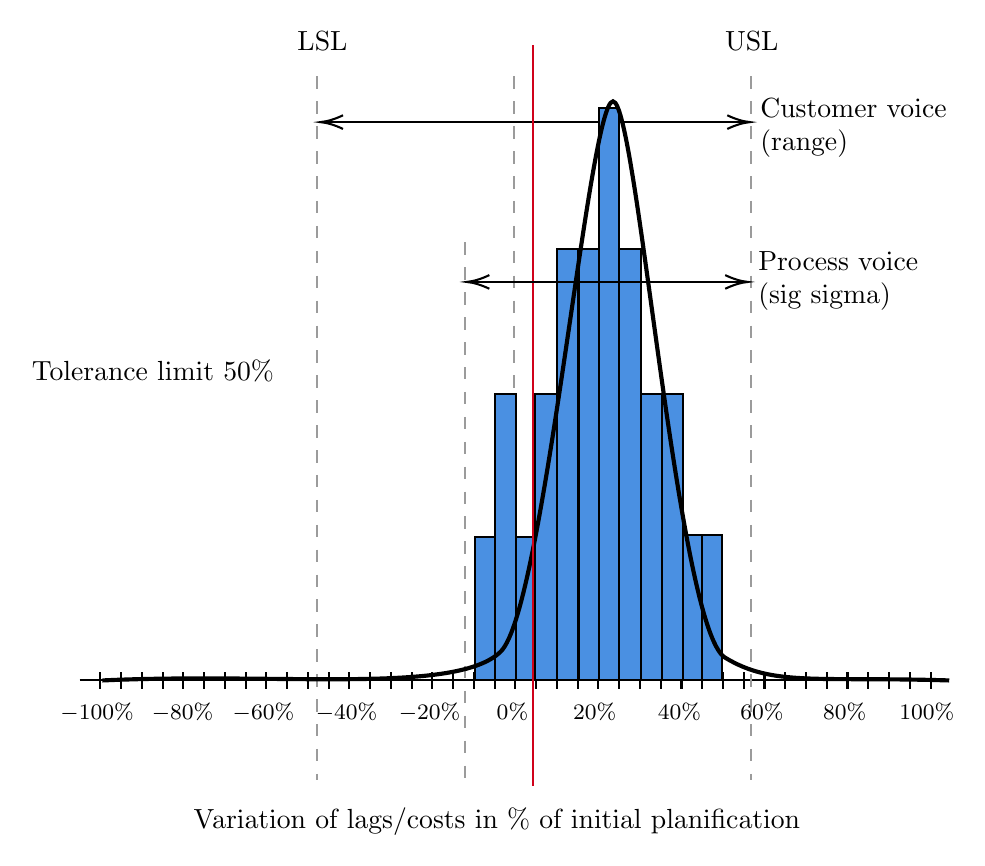
\begin{tikzpicture}[x=0.75pt,y=0.75pt,yscale=-1,xscale=1]
		%uncomment if require: \path (0,896); %set diagram left start at 0, and has height of 896
		
		%Straight Lines [id:da4860615708244953] 
		\draw    (126.5,373) -- (545.5,373) (136.5,369) -- (136.5,377)(146.5,369) -- (146.5,377)(156.5,369) -- (156.5,377)(166.5,369) -- (166.5,377)(176.5,369) -- (176.5,377)(186.5,369) -- (186.5,377)(196.5,369) -- (196.5,377)(206.5,369) -- (206.5,377)(216.5,369) -- (216.5,377)(226.5,369) -- (226.5,377)(236.5,369) -- (236.5,377)(246.5,369) -- (246.5,377)(256.5,369) -- (256.5,377)(266.5,369) -- (266.5,377)(276.5,369) -- (276.5,377)(286.5,369) -- (286.5,377)(296.5,369) -- (296.5,377)(306.5,369) -- (306.5,377)(316.5,369) -- (316.5,377)(326.5,369) -- (326.5,377)(336.5,369) -- (336.5,377)(346.5,369) -- (346.5,377)(356.5,369) -- (356.5,377)(366.5,369) -- (366.5,377)(376.5,369) -- (376.5,377)(386.5,369) -- (386.5,377)(396.5,369) -- (396.5,377)(406.5,369) -- (406.5,377)(416.5,369) -- (416.5,377)(426.5,369) -- (426.5,377)(436.5,369) -- (436.5,377)(446.5,369) -- (446.5,377)(456.5,369) -- (456.5,377)(466.5,369) -- (466.5,377)(476.5,369) -- (476.5,377)(486.5,369) -- (486.5,377)(496.5,369) -- (496.5,377)(506.5,369) -- (506.5,377)(516.5,369) -- (516.5,377)(526.5,369) -- (526.5,377)(536.5,369) -- (536.5,377) ;
		%Straight Lines [id:da9174452977196303] 
		\draw [color={rgb, 255:red, 155; green, 155; blue, 155 }  ,draw opacity=1 ] [dash pattern={on 4.5pt off 4.5pt}]  (336,82) -- (336,373) ;
		%Straight Lines [id:da6722948113064402] 
		\draw [color={rgb, 255:red, 155; green, 155; blue, 155 }  ,draw opacity=1 ] [dash pattern={on 4.5pt off 4.5pt}]  (312,162) -- (312,421) ;
		%Straight Lines [id:da38389428223380206] 
		\draw [color={rgb, 255:red, 155; green, 155; blue, 155 }  ,draw opacity=1 ] [dash pattern={on 4.5pt off 4.5pt}]  (450,82) -- (450,421) ;
		%Straight Lines [id:da7747556344857307] 
		\draw [color={rgb, 255:red, 155; green, 155; blue, 155 }  ,draw opacity=1 ] [dash pattern={on 4.5pt off 4.5pt}]  (241,82) -- (241,421) ;
		%Straight Lines [id:da41615772845726884] 
		\draw    (244.5,104) -- (447.5,104) ;
		\draw [shift={(449.5,104)}, rotate = 180] [color={rgb, 255:red, 0; green, 0; blue, 0 }  ][line width=0.75]    (10.93,-3.29) .. controls (6.95,-1.4) and (3.31,-0.3) .. (0,0) .. controls (3.31,0.3) and (6.95,1.4) .. (10.93,3.29)   ;
		\draw [shift={(242.5,104)}, rotate = 0] [color={rgb, 255:red, 0; green, 0; blue, 0 }  ][line width=0.75]    (10.93,-3.29) .. controls (6.95,-1.4) and (3.31,-0.3) .. (0,0) .. controls (3.31,0.3) and (6.95,1.4) .. (10.93,3.29)   ;
		%Shape: Rectangle [id:dp9272741577539436] 
		\draw  [fill={rgb, 255:red, 74; green, 144; blue, 226 }  ,fill opacity=1 ] (317,304) -- (326.5,304) -- (326.5,373) -- (317,373) -- cycle ;
		%Shape: Rectangle [id:dp6111436200810569] 
		\draw  [fill={rgb, 255:red, 74; green, 144; blue, 226 }  ,fill opacity=1 ] (326.5,235) -- (336.8,235) -- (336.8,373) -- (326.5,373) -- cycle ;
		%Shape: Rectangle [id:dp45902692323790895] 
		\draw  [fill={rgb, 255:red, 74; green, 144; blue, 226 }  ,fill opacity=1 ] (336.8,304) -- (346,304) -- (346,373) -- (336.8,373) -- cycle ;
		%Shape: Rectangle [id:dp5007198507349022] 
		\draw  [fill={rgb, 255:red, 74; green, 144; blue, 226 }  ,fill opacity=1 ] (346,235) -- (356.4,235) -- (356.4,373) -- (346,373) -- cycle ;
		%Shape: Rectangle [id:dp8282203264299566] 
		\draw  [fill={rgb, 255:red, 74; green, 144; blue, 226 }  ,fill opacity=1 ] (356.4,165) -- (366.9,165) -- (366.9,373) -- (356.4,373) -- cycle ;
		%Shape: Rectangle [id:dp5243868889045202] 
		\draw  [fill={rgb, 255:red, 74; green, 144; blue, 226 }  ,fill opacity=1 ] (366.9,165) -- (376.8,165) -- (376.8,373) -- (366.9,373) -- cycle ;
		%Shape: Rectangle [id:dp3821757031461548] 
		\draw  [fill={rgb, 255:red, 74; green, 144; blue, 226 }  ,fill opacity=1 ] (376.8,97) -- (386.3,97) -- (386.3,373) -- (376.8,373) -- cycle ;
		%Shape: Rectangle [id:dp16293254752754316] 
		\draw  [fill={rgb, 255:red, 74; green, 144; blue, 226 }  ,fill opacity=1 ] (386.3,165) -- (396.8,165) -- (396.8,373) -- (386.3,373) -- cycle ;
		%Shape: Rectangle [id:dp4965179570774956] 
		\draw  [fill={rgb, 255:red, 74; green, 144; blue, 226 }  ,fill opacity=1 ] (396.8,235) -- (407.2,235) -- (407.2,373) -- (396.8,373) -- cycle ;
		%Shape: Rectangle [id:dp7777494083675129] 
		\draw  [fill={rgb, 255:red, 74; green, 144; blue, 226 }  ,fill opacity=1 ] (407.2,235) -- (417.2,235) -- (417.2,373) -- (407.2,373) -- cycle ;
		%Shape: Rectangle [id:dp6948842502676678] 
		\draw  [fill={rgb, 255:red, 74; green, 144; blue, 226 }  ,fill opacity=1 ] (417.2,303) -- (426.4,303) -- (426.4,373) -- (417.2,373) -- cycle ;
		%Shape: Rectangle [id:dp43361616314907137] 
		\draw  [fill={rgb, 255:red, 74; green, 144; blue, 226 }  ,fill opacity=1 ] (426.4,303) -- (435.9,303) -- (435.9,373) -- (426.4,373) -- cycle ;
		%Curve Lines [id:da0695114930547609] 
		\draw [color={rgb, 255:red, 0; green, 0; blue, 0 }  ,draw opacity=1 ][line width=1.5]    (137.5,373) .. controls (223.5,369) and (308.5,380) .. (329.5,359) .. controls (350.5,338) and (371.9,94) .. (383.5,94) .. controls (395.1,94) and (414.5,348) .. (437.5,362) .. controls (460.5,376) and (481.5,371) .. (545.5,373) ;
		%Straight Lines [id:da8097631673347889] 
		\draw [color={rgb, 255:red, 208; green, 2; blue, 27 }  ,draw opacity=1 ]   (345,67) -- (345,424) ;
		%Straight Lines [id:da3745662432657628] 
		\draw    (315,181) -- (446.5,181) ;
		\draw [shift={(448.5,181)}, rotate = 180] [color={rgb, 255:red, 0; green, 0; blue, 0 }  ][line width=0.75]    (10.93,-3.29) .. controls (6.95,-1.4) and (3.31,-0.3) .. (0,0) .. controls (3.31,0.3) and (6.95,1.4) .. (10.93,3.29)   ;
		\draw [shift={(313,181)}, rotate = 0] [color={rgb, 255:red, 0; green, 0; blue, 0 }  ][line width=0.75]    (10.93,-3.29) .. controls (6.95,-1.4) and (3.31,-0.3) .. (0,0) .. controls (3.31,0.3) and (6.95,1.4) .. (10.93,3.29)   ;
		
		% Text Node
		\draw (326,382.4) node [anchor=north west][inner sep=0.75pt]  [font=\footnotesize]  {$0\%$};
		% Text Node
		\draw (362.8,382.4) node [anchor=north west][inner sep=0.75pt]  [font=\footnotesize]  {$20\%$};
		% Text Node
		\draw (403.6,382.4) node [anchor=north west][inner sep=0.75pt]  [font=\footnotesize]  {$40\%$};
		% Text Node
		\draw (443.4,382.4) node [anchor=north west][inner sep=0.75pt]  [font=\footnotesize]  {$60\%$};
		% Text Node
		\draw (483.2,382.4) node [anchor=north west][inner sep=0.75pt]  [font=\footnotesize]  {$80\%$};
		% Text Node
		\draw (520,382.4) node [anchor=north west][inner sep=0.75pt]  [font=\footnotesize]  {$100\%$};
		% Text Node
		\draw (278.8,382.4) node [anchor=north west][inner sep=0.75pt]  [font=\footnotesize]  {$-20\%$};
		% Text Node
		\draw (238.8,382.4) node [anchor=north west][inner sep=0.75pt]  [font=\footnotesize]  {$-40\%$};
		% Text Node
		\draw (198.8,382.4) node [anchor=north west][inner sep=0.75pt]  [font=\footnotesize]  {$-60\%$};
		% Text Node
		\draw (159.8,382.4) node [anchor=north west][inner sep=0.75pt]  [font=\footnotesize]  {$-80\%$};
		% Text Node
		\draw (115.8,382.4) node [anchor=north west][inner sep=0.75pt]  [font=\footnotesize]  {$-100\%$};
		% Text Node
		\draw (452,165) node [anchor=north west][inner sep=0.75pt]   [align=left] {Process voice\\(sig sigma)};
		% Text Node
		\draw (436,59) node [anchor=north west][inner sep=0.75pt]   [align=left] {USL};
		% Text Node
		\draw (230,59) node [anchor=north west][inner sep=0.75pt]   [align=left] {LSL};
		% Text Node
		\draw (453,91) node [anchor=north west][inner sep=0.75pt]   [align=left] {Customer voice\\(range)};
		% Text Node
		\draw (102,217) node [anchor=north west][inner sep=0.75pt]   [align=left] {Tolerance limit $\displaystyle 50\%$};
		% Text Node
		\draw (180,433) node [anchor=north west][inner sep=0.75pt]   [align=left] {Variation of lags/costs in $\displaystyle \%$ of initial planification};
		\end{tikzpicture}
		\vspace*{3mm}
		\caption{Example of typical histogram in engineering companies (Six Sigma)}
	\end{figure}	
	Histograms allow to observe distributions and determine qualitatively if it fits a particular theoretical model.
	
	Graphics can also be used to observe changes over time (time series, control charts, residual analysis, etc.):
	
	\begin{figure}[H]
		\centering
		\includegraphics[scale=0.75]{img/analysis/time_serie.eps}
		\caption{Example of OHLC (candlestick plot) time series with moving averages in financial trading}
	\end{figure}
	or another type of OHLC (Open-High-Low-Close) trading plot:
	\begin{figure}[H]
		\centering
		\includegraphics[scale=0.75]{img/analysis/plot_OHLC.jpg}
	\end{figure}
	There are different rules for the colors of an OHLC plot! We can first define a color depending if the close price is lower than the open price \underline{of the same symbol/candlestick} (the open price is always on the left and the closure price always on the right):
	\begin{figure}[H]
		\centering
		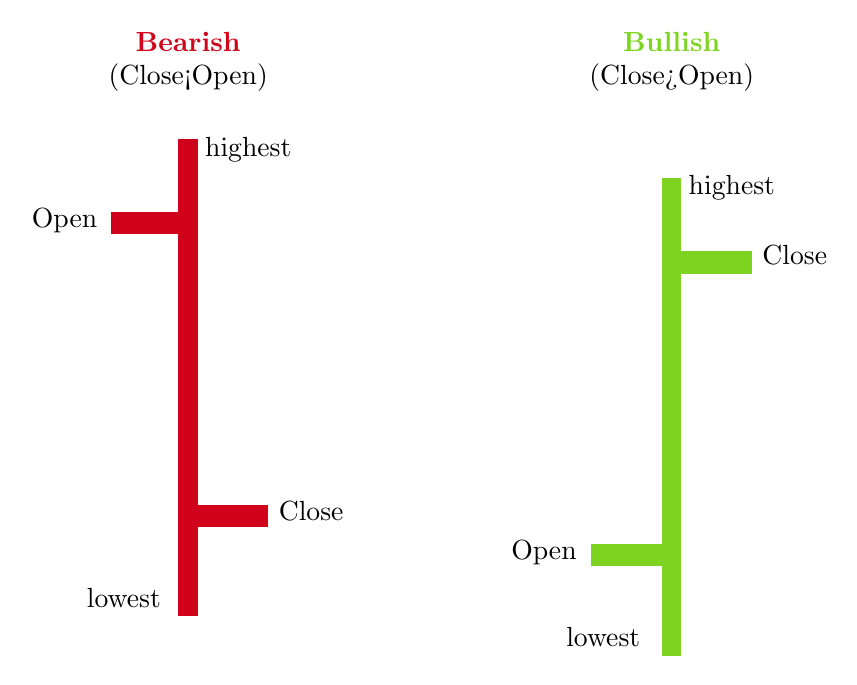
\begin{tikzpicture}[x=0.75pt,y=0.75pt,yscale=-1,xscale=1]
		%uncomment if require: \path (0,1046); %set diagram left start at 0, and has height of 1046
		
		%Shape: Rectangle [id:dp11276901412130624] 
		\draw  [draw opacity=0][fill={rgb, 255:red, 208; green, 2; blue, 27 }  ,fill opacity=1 ] (195,139) -- (204.5,139) -- (204.5,369) -- (195,369) -- cycle ;
		%Shape: Rectangle [id:dp3380346726998751] 
		\draw  [draw opacity=0][fill={rgb, 255:red, 208; green, 2; blue, 27 }  ,fill opacity=1 ] (201.5,174.25) -- (201.5,185) -- (162.75,185) -- (162.75,174.25) -- cycle ;
		%Shape: Rectangle [id:dp05932809183106258] 
		\draw  [draw opacity=0][fill={rgb, 255:red, 208; green, 2; blue, 27 }  ,fill opacity=1 ] (238.5,315.25) -- (238.5,326) -- (199.75,326) -- (199.75,315.25) -- cycle ;
		%Shape: Rectangle [id:dp9748292520522313] 
		\draw  [draw opacity=0][fill={rgb, 255:red, 126; green, 211; blue, 33 }  ,fill opacity=1 ] (428,158) -- (437.5,158) -- (437.5,388) -- (428,388) -- cycle ;
		%Shape: Rectangle [id:dp2419070119256983] 
		\draw  [draw opacity=0][fill={rgb, 255:red, 126; green, 211; blue, 33 }  ,fill opacity=1 ] (471.5,193.25) -- (471.5,204) -- (432.75,204) -- (432.75,193.25) -- cycle ;
		%Shape: Rectangle [id:dp6165629355003259] 
		\draw  [draw opacity=0][fill={rgb, 255:red, 126; green, 211; blue, 33 }  ,fill opacity=1 ] (432.5,334.25) -- (432.5,345) -- (393.75,345) -- (393.75,334.25) -- cycle ;
		
		% Text Node
		\draw (154,86) node [anchor=north west][inner sep=0.75pt]   [align=left] {\begin{minipage}[lt]{66.5pt}\setlength\topsep{0pt}
		\begin{center}
		\textbf{\textcolor[rgb]{0.82,0.01,0.11}{Bearish}}\\(Close<Open)
		\end{center}
		
		\end{minipage}};
		% Text Node
		\draw (387,86) node [anchor=north west][inner sep=0.75pt]   [align=left] {\begin{minipage}[lt]{66.5pt}\setlength\topsep{0pt}
		\begin{center}
		\textbf{\textcolor[rgb]{0.49,0.83,0.13}{Bullish}}\\(Close>Open)
		\end{center}
		
		\end{minipage}};
		% Text Node
		\draw (123,171) node [anchor=north west][inner sep=0.75pt]   [align=left] {Open};
		% Text Node
		\draw (354,331) node [anchor=north west][inner sep=0.75pt]   [align=left] {Open};
		% Text Node
		\draw (242,312) node [anchor=north west][inner sep=0.75pt]   [align=left] {Close};
		% Text Node
		\draw (475,189) node [anchor=north west][inner sep=0.75pt]   [align=left] {Close};
		% Text Node
		\draw (206.5,137) node [anchor=north west][inner sep=0.75pt]   [align=left] {highest};
		% Text Node
		\draw (149.5,354) node [anchor=north west][inner sep=0.75pt]   [align=left] {lowest};
		% Text Node
		\draw (380.5,373) node [anchor=north west][inner sep=0.75pt]   [align=left] {lowest};
		% Text Node
		\draw (439.5,155) node [anchor=north west][inner sep=0.75pt]   [align=left] {highest};
		
		\end{tikzpicture}
	\end{figure}
	A common question related to this chart is: \textit{Why doesn't a candlestick open when another one closes?}
	
	This is because the close price is created by the last tick of clock to arrive before the end of the candles time period, this may be several seconds before the end of the candles time period. The next candles open price is generated by the first tick of the clock to arrive after the beginning of its time period, this tick will reflect a change in price since the tick that generated the close price of the last candle, this first tick of the new candle may be several seconds after the beginning of the candles time period.
	
	And still many other charts... that we have already seen and others that we will see throughout the pages of this book.

	\paragraph{3D representations}\mbox{}\\\\
	Of course, in the case of a trivalent function (three-dimensional), that is to say a parameter which depends on two other, the idea is the same as for 2D except that the number of quadrants doubles:
	\begin{figure}[H]
		\centering
		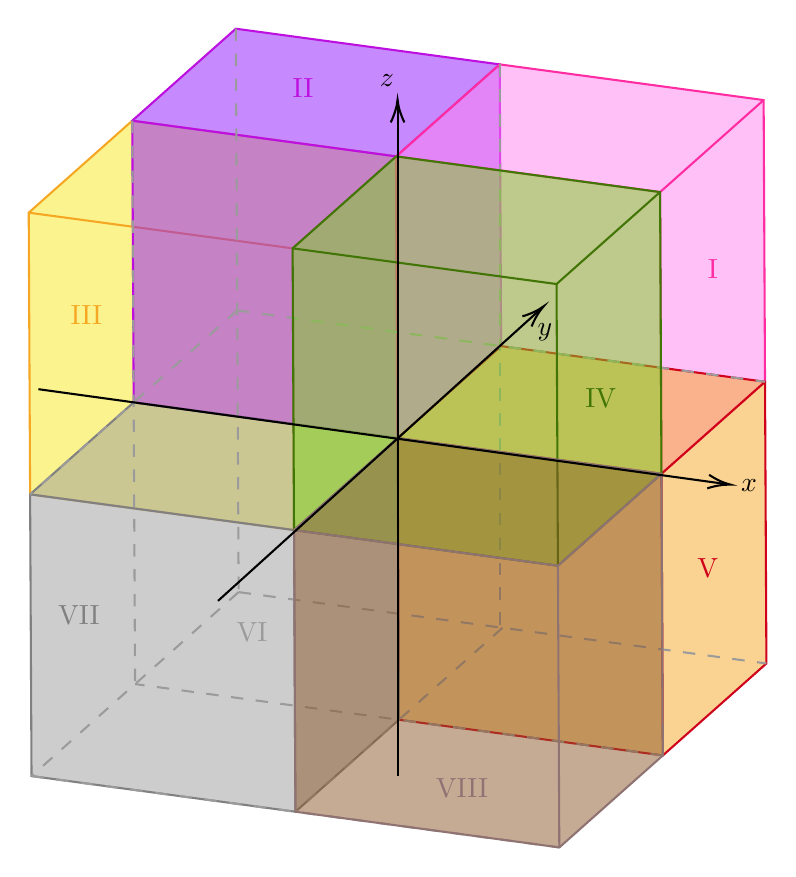
\begin{tikzpicture}[x=0.75pt,y=0.75pt,yscale=-1,xscale=1]
		%uncomment if require: \path (0,1215); %set diagram left start at 0, and has height of 1215
		
		%Shape: Cube [id:dp7756626769195145] 
		\draw  [color={rgb, 255:red, 245; green, 166; blue, 35 }  ,draw opacity=1 ][fill={rgb, 255:red, 248; green, 231; blue, 28 }  ,fill opacity=0.5 ] (170.32,132.95) -- (220.21,88.64) -- (347.36,105.83) -- (348.03,241.54) -- (298.14,285.86) -- (170.99,268.67) -- cycle ; \draw  [color={rgb, 255:red, 245; green, 166; blue, 35 }  ,draw opacity=1 ] (347.36,105.83) -- (297.47,150.14) -- (170.32,132.95) ; \draw  [color={rgb, 255:red, 245; green, 166; blue, 35 }  ,draw opacity=1 ] (297.47,150.14) -- (298.14,285.86) ;
		%Shape: Cube [id:dp967030549945288] 
		\draw  [color={rgb, 255:red, 189; green, 16; blue, 224 }  ,draw opacity=1 ][fill={rgb, 255:red, 144; green, 19; blue, 254 }  ,fill opacity=0.5 ] (220.21,88.64) -- (270.1,44.32) -- (397.25,61.51) -- (397.92,197.23) -- (348.03,241.54) -- (220.88,224.35) -- cycle ; \draw  [color={rgb, 255:red, 189; green, 16; blue, 224 }  ,draw opacity=1 ] (397.25,61.51) -- (347.36,105.83) -- (220.21,88.64) ; \draw  [color={rgb, 255:red, 189; green, 16; blue, 224 }  ,draw opacity=1 ] (347.36,105.83) -- (348.03,241.54) ;
		%Shape: Cube [id:dp9831133876362679] 
		\draw  [color={rgb, 255:red, 255; green, 44; blue, 162 }  ,draw opacity=1 ][fill={rgb, 255:red, 255; green, 128; blue, 240 }  ,fill opacity=0.5 ] (347.36,105.83) -- (397.25,61.51) -- (524.4,78.7) -- (525.07,214.42) -- (475.18,258.74) -- (348.03,241.54) -- cycle ; \draw  [color={rgb, 255:red, 255; green, 44; blue, 162 }  ,draw opacity=1 ] (524.4,78.7) -- (474.51,123.02) -- (347.36,105.83) ; \draw  [color={rgb, 255:red, 255; green, 44; blue, 162 }  ,draw opacity=1 ] (474.51,123.02) -- (475.18,258.74) ;
		%Shape: Cube [id:dp7548991045714146] 
		\draw  [color={rgb, 255:red, 208; green, 2; blue, 27 }  ,draw opacity=1 ][fill={rgb, 255:red, 245; green, 166; blue, 35 }  ,fill opacity=0.5 ] (348.03,241.54) -- (397.92,197.23) -- (525.07,214.42) -- (525.74,350.14) -- (475.85,394.45) -- (348.7,377.26) -- cycle ; \draw  [color={rgb, 255:red, 208; green, 2; blue, 27 }  ,draw opacity=1 ] (525.07,214.42) -- (475.18,258.74) -- (348.03,241.54) ; \draw  [color={rgb, 255:red, 208; green, 2; blue, 27 }  ,draw opacity=1 ] (475.18,258.74) -- (475.85,394.45) ;
		%Shape: Cube [id:dp23144213220997512] 
		\draw  [color={rgb, 255:red, 128; green, 128; blue, 128 }  ,draw opacity=1 ][fill={rgb, 255:red, 155; green, 155; blue, 155 }  ,fill opacity=0.5 ] (170.99,268.67) -- (220.88,224.35) -- (348.03,241.54) -- (348.7,377.26) -- (298.81,421.57) -- (171.67,404.38) -- cycle ; \draw  [color={rgb, 255:red, 128; green, 128; blue, 128 }  ,draw opacity=1 ] (348.03,241.54) -- (298.14,285.86) -- (170.99,268.67) ; \draw  [color={rgb, 255:red, 128; green, 128; blue, 128 }  ,draw opacity=1 ] (298.14,285.86) -- (298.81,421.57) ;
		%Straight Lines [id:da7814625435812566] 
		\draw [color={rgb, 255:red, 155; green, 155; blue, 155 }  ,draw opacity=1 ] [dash pattern={on 4.5pt off 4.5pt}]  (171.67,404.38) -- (425.96,438.77) ;
		%Straight Lines [id:da20201785751326806] 
		\draw [color={rgb, 255:red, 155; green, 155; blue, 155 }  ,draw opacity=1 ] [dash pattern={on 4.5pt off 4.5pt}]  (271.45,315.76) -- (525.74,350.14) ;
		%Straight Lines [id:da8736466171243731] 
		\draw [color={rgb, 255:red, 155; green, 155; blue, 155 }  ,draw opacity=1 ] [dash pattern={on 4.5pt off 4.5pt}]  (271.45,315.76) -- (171.67,404.38) ;
		%Straight Lines [id:da020932833087546676] 
		\draw [color={rgb, 255:red, 155; green, 155; blue, 155 }  ,draw opacity=1 ] [dash pattern={on 4.5pt off 4.5pt}]  (270.1,44.32) -- (271.45,315.76) ;
		%Straight Lines [id:da37372574513823675] 
		\draw [color={rgb, 255:red, 155; green, 155; blue, 155 }  ,draw opacity=1 ] [dash pattern={on 4.5pt off 4.5pt}]  (475.85,394.45) -- (221.56,360.07) ;
		%Straight Lines [id:da6873190478300943] 
		\draw [color={rgb, 255:red, 155; green, 155; blue, 155 }  ,draw opacity=1 ] [dash pattern={on 4.5pt off 4.5pt}]  (220.21,88.64) -- (221.56,360.07) ;
		%Straight Lines [id:da42663298987935616] 
		\draw [color={rgb, 255:red, 155; green, 155; blue, 155 }  ,draw opacity=1 ] [dash pattern={on 4.5pt off 4.5pt}]  (398.59,332.95) -- (298.81,421.57) ;
		%Straight Lines [id:da6444781166785933] 
		\draw [color={rgb, 255:red, 155; green, 155; blue, 155 }  ,draw opacity=1 ] [dash pattern={on 4.5pt off 4.5pt}]  (270.77,180.04) -- (525.07,214.42) ;
		%Straight Lines [id:da7845775656184948] 
		\draw [color={rgb, 255:red, 155; green, 155; blue, 155 }  ,draw opacity=1 ] [dash pattern={on 4.5pt off 4.5pt}]  (270.77,180.04) -- (170.99,268.67) ;
		%Straight Lines [id:da9856171255690882] 
		\draw [color={rgb, 255:red, 155; green, 155; blue, 155 }  ,draw opacity=1 ] [dash pattern={on 4.5pt off 4.5pt}]  (397.25,61.51) -- (397.25,332.95) ;
		%Shape: Cube [id:dp24967959490129488] 
		\draw  [color={rgb, 255:red, 65; green, 117; blue, 5 }  ,draw opacity=1 ][fill={rgb, 255:red, 126; green, 211; blue, 33 }  ,fill opacity=0.5 ] (297.47,150.14) -- (347.36,105.83) -- (474.51,123.02) -- (475.18,258.74) -- (425.29,303.05) -- (298.14,285.86) -- cycle ; \draw  [color={rgb, 255:red, 65; green, 117; blue, 5 }  ,draw opacity=1 ] (474.51,123.02) -- (424.62,167.33) -- (297.47,150.14) ; \draw  [color={rgb, 255:red, 65; green, 117; blue, 5 }  ,draw opacity=1 ] (424.62,167.33) -- (425.29,303.05) ;
		%Shape: Cube [id:dp9214352067443166] 
		\draw  [color={rgb, 255:red, 143; green, 115; blue, 115 }  ,draw opacity=1 ][fill={rgb, 255:red, 139; green, 87; blue, 42 }  ,fill opacity=0.5 ] (298.14,285.86) -- (348.03,241.54) -- (475.18,258.74) -- (475.85,394.45) -- (425.96,438.77) -- (298.81,421.57) -- cycle ; \draw  [color={rgb, 255:red, 143; green, 115; blue, 115 }  ,draw opacity=1 ] (475.18,258.74) -- (425.29,303.05) -- (298.14,285.86) ; \draw  [color={rgb, 255:red, 143; green, 115; blue, 115 }  ,draw opacity=1 ] (425.29,303.05) -- (425.96,438.77) ;
		%Straight Lines [id:da6079877488392815] 
		\draw    (175,218) -- (506.52,263.73) ;
		\draw [shift={(508.5,264)}, rotate = 187.85] [color={rgb, 255:red, 0; green, 0; blue, 0 }  ][line width=0.75]    (10.93,-3.29) .. controls (6.95,-1.4) and (3.31,-0.3) .. (0,0) .. controls (3.31,0.3) and (6.95,1.4) .. (10.93,3.29)   ;
		%Straight Lines [id:da2944625983593221] 
		\draw    (348.03,404.54) -- (348.03,80.54) ;
		\draw [shift={(348.03,78.54)}, rotate = 90] [color={rgb, 255:red, 0; green, 0; blue, 0 }  ][line width=0.75]    (10.93,-3.29) .. controls (6.95,-1.4) and (3.31,-0.3) .. (0,0) .. controls (3.31,0.3) and (6.95,1.4) .. (10.93,3.29)   ;
		%Straight Lines [id:da842300970026929] 
		\draw    (261.5,320) -- (417.02,179.34) ;
		\draw [shift={(418.5,178)}, rotate = 137.87] [color={rgb, 255:red, 0; green, 0; blue, 0 }  ][line width=0.75]    (10.93,-3.29) .. controls (6.95,-1.4) and (3.31,-0.3) .. (0,0) .. controls (3.31,0.3) and (6.95,1.4) .. (10.93,3.29)   ;
		
		% Text Node
		\draw (338,65) node [anchor=north west][inner sep=0.75pt]    {$z$};
		% Text Node
		\draw (512,260) node [anchor=north west][inner sep=0.75pt]    {$x$};
		% Text Node
		\draw (414,185) node [anchor=north west][inner sep=0.75pt]    {$y$};
		% Text Node
		\draw (296,67) node [anchor=north west][inner sep=0.75pt]  [color={rgb, 255:red, 189; green, 16; blue, 224 }  ,opacity=1 ] [align=left] {II};
		% Text Node
		\draw (496,154) node [anchor=north west][inner sep=0.75pt]  [color={rgb, 255:red, 255; green, 44; blue, 162 }  ,opacity=1 ] [align=left] {I};
		% Text Node
		\draw (437,216) node [anchor=north west][inner sep=0.75pt]  [color={rgb, 255:red, 65; green, 117; blue, 5 }  ,opacity=1 ] [align=left] {IV};
		% Text Node
		\draw (189,176) node [anchor=north west][inner sep=0.75pt]  [color={rgb, 255:red, 245; green, 166; blue, 35 }  ,opacity=1 ] [align=left] {III};
		% Text Node
		\draw (491,298) node [anchor=north west][inner sep=0.75pt]  [color={rgb, 255:red, 208; green, 2; blue, 27 }  ,opacity=1 ] [align=left] {V};
		% Text Node
		\draw (269,329) node [anchor=north west][inner sep=0.75pt]  [color={rgb, 255:red, 155; green, 155; blue, 155 }  ,opacity=1 ] [align=left] {VI};
		% Text Node
		\draw (365,404) node [anchor=north west][inner sep=0.75pt]  [color={rgb, 255:red, 143; green, 115; blue, 115 }  ,opacity=1 ] [align=left] {VIII};
		% Text Node
		\draw (183,321) node [anchor=north west][inner sep=0.75pt]  [color={rgb, 255:red, 128; green, 128; blue, 128 }  ,opacity=1 ] [align=left] {VII};
		\end{tikzpicture}
		\vspace*{3mm}
		\caption[Quadrants in a 3D orthogonal system]{Quadrants in a 3D orthogonal system (source: Wikipedia)}
	\end{figure}
	
	This 3D method of representation and analysis of a trivalent function was time consuming at the beginning of the 120th century (holocene calendar) but with the help of computers in the end of the 120th century this time consuming problem was almost solved...
	
	In 3D functional analysis, we will deal with functions of two or three variables (usually $x, y, z$, respectively). The graph of the arrow of coordinates $(x, y, z)=(x,y,f(x,y))$, lies in the Euclidean space. Since the Euclidean space can be $3$-dimensional (and more or less for sure!), we denote it by $\mathbb{R}^3$.
	
	Euclidean space has three mutually perpendicular coordinate axes ($x$, $y$ and $z$), and three mutually perpendicular coordinate planes: the $xy$-plane, $yz$-plane and $xz$-plane:

	\begin{figure}[H]
		\centering
		\tdplotsetmaincoords{60}{130}
		\begin{tikzpicture}[scale = 5, tdplot_main_coords]
			
			\coordinate (O) at (0,0,0);
			\coordinate (x) at (1,0,0);
			\coordinate (y) at (0,1,0);
			\coordinate (z) at (0,0,1);
			
			\draw[thick, >=Stealth, ->] (O) -- (x) node[anchor = north]{$x$}; % x
			\draw[thick, >=Stealth, ->] (O) -- (y) node[anchor = north]{$y$}; % y
			\draw[thick, >=Stealth, ->] (O) -- (z) node[anchor = south]{$z$}; % z
			
			\coordinate (xz) at (1,0,1);
			\coordinate (yz) at (0,1,1);
			\coordinate (xy) at (1,1,0);
			
			
			% text on the xy plane; the following line does not work.
			% \draw[canvas is xy plane at z = 0, draw = red, fill = red!50, opacity = 0.5] (xy) rectangle (O);
			\filldraw[fill = green!50, opacity = 0.5] (xy) -- (x) -- (O) -- (y) -- cycle;
			\node[canvas is xy plane at z = 0] at (0.5,0.5,0) {$xy$ plane};
			
			% text on the yz plane
			\draw[canvas is yz plane at x = 0, transform shape, draw = red, fill = red!50, opacity = 0.5] (yz) rectangle (O);
			\node[canvas is yz plane at x = 0] at (0,0.5,0.5) {$yz$ plane};
			
			% text on the xz plane (Notice: it seems that the text has been reflected)
			\draw[canvas is xz plane at y = 0, transform shape, draw = blue, fill = blue!50, opacity = 0.5] (xz) rectangle (O);
			\node[canvas is xz plane at y = 0] at (0.5,0,0.5){\reflectbox{$xz$ plane}};
			\node at (0,-0.1) {O};
		\end{tikzpicture}
		\vspace*{3mm}
		\caption{Mutually perpendicular planes in $\mathbb{R}^3$}
	\end{figure}

	The coordinate system shown above is known as a right-handed coordinate system, because it is possible, using the right hand, to point the index finger in the positive direction of the $x$-axis, the middle finger in the positive direction of the $y$-axis, and the thumb in the positive direction of the $z$-axis, as below:

	\begin{figure}[H]
		\centering
		% RIGHT HAND RULE xyz
		\begin{tikzpicture}
		\colorlet{pinkskin}{pink!25}
		\colorlet{brownskin}{pink!5!brown!45}
		\colorlet{myred}{red!90!black}
		\colorlet{myblue}{blue!90!black}
		\colorlet{mypurple}{blue!50!red!80!black!80}
		\colorlet{Bcol}{violet!90}
		\colorlet{BFcol}{red!60!black}
		\colorlet{veccol}{green!45!black}
		\colorlet{Icol}{blue!70!black}
		\colorlet{mucol}{red!90!black}
		\tikzstyle{BField}=[->,line width=2,Bcol]
		\tikzstyle{current}=[->,Icol] %thick,
		\tikzstyle{force}=[->,line width=2,BFcol]
		\tikzstyle{vector}=[->,line width=2,veccol]
		\tikzstyle{thick vector}=[->,line width=2,veccol]
		\tikzstyle{mu vector}=[->,line width=2,mucol]
		\tikzstyle{velocity}=[->,line width=2,veccol]
		\tikzstyle{charge+}=[very thin,draw=black,top color=red!50,bottom color=red!90!black,shading angle=20,circle,inner sep=0.5]
		  \coordinate (O) at (1.0,0.7); % ORIGIN
		  \coordinate (WT) at ( 2.9,-1.1); % WRIST TOP
		  \coordinate (T1) at ( 2.3, 0.7); % THUMB
		  \coordinate (T2) at ( 1.75, 2.3);
		  \coordinate (T3) at ( 2.0, 3.1);
		  \coordinate (T4) at (1.38, 3.15);
		  \coordinate (T5) at ( 0.9, 2.3);
		  \coordinate (T6) at ( 0.85, 1.2);
		  \coordinate (T7) at ( 0.85, 0.2);
		  \coordinate (I1) at (-1.1, 2.45); % INDEX
		  \coordinate (I2) at (-2.9, 3.45);
		  \coordinate (I3) at (-3.3, 2.9);
		  \coordinate (I4) at (-1.5, 1.8);
		  \coordinate (I5) at (-0.9, 1.1);
		  \coordinate (I6) at (-0.9, 0.3);
		  \coordinate (M1) at (-2.1, 0.9); % MIDDLE
		  \coordinate (M2) at (-3.95,0.55);
		  \coordinate (M3) at (-4.0,-0.15);
		  \coordinate (M4) at (-2.3, 0.05);
		  \coordinate (M5) at (-1.1, 0.20);
		  \coordinate (R1) at (-1.9,-0.1); % RING
		  \coordinate (R2) at (-1.8,-0.7);
		  \coordinate (R3) at (-0.3,-1.5);
		  \coordinate (R4) at ( 0.1,-1.7);
		  \coordinate (R5) at ( 0.1,-1.0);
		  \coordinate (R6) at (-0.5,-0.7);
		  \coordinate (R7) at (-1.2,-0.3);
		  \coordinate (P1) at (-1.9,-1.3); % PINKY
		  \coordinate (P2) at (-0.8,-1.9);
		  \coordinate (P3) at (-0.2,-2.1);
		  \coordinate (P4) at (-0.05,-1.65);
		  \coordinate (W1) at ( 0.4,-2.9); % WRIST BOTTOM
		  \coordinate (W2) at ( 1.6,-3.5);
		  
		  % HAND
		  \fill[pinkskin]
		    (WT) -- (T6) -- (I5) -- (M5) -- (R2) -- (P2) -- (W2) to[out=25,in=-90] cycle;
		  \draw[fill=pinkskin]
		    (WT) to[out=120,in=-60] % THUMB
		    (T1) to[out=120,in=-90]
		    (T2) to[out=80,in=-110]
		    (T3) to[out=80,in=50,looseness=1.5] % tip
		    (T4) to[out=-130,in=80]
		    (T5) to[out=-100,in=70]
		    (T6) to[out=-100,in=100]
		    (T7)
		    (T6) to[out=150,in=-30] % INDEX
		    (I1) to[out=150,in=-30]
		    (I2) to[out=150,in=145,looseness=1.7] % tip
		    (I3) to[out=-30,in=150]
		    (I4) to[out=-30,in=105]
		    (I5) to[out=-75,in=90]
		    (I6)
		    (I5) to[out=-170,in=10] % MIDDLE
		    (M1) to[out=-170,in=10]
		    (M2) to[out=-170,in=-175,looseness=1.8] % tip
		    (M3) to[out=5,in=-170]
		    (M4) to[out=10,in=-170] % bottom knuckle
		    (M5)
		    (M5) to[out=-160,in=50] % RING
		    (R1) to[out=-130,in=140,looseness=1.2]
		    (R2) to[out=-30,in=160]
		    (R3) --
		    (R4) to[out=-20,in=-20,looseness=1.5] % tip
		    (R5) --
		    (R6) to[out=140,in=8,looseness=0.9]
		    (R7)
		    (R2) to[out=-160,in=155] % PINKY
		    (P1) to[out=-35,in=150]
		    (P2) to[out=-30,in=160]
		    (P3) to[out=-20,in=-30,looseness=1.5] % tip
		    %(P4) --
		    (R4)
		    (P2) to[out=-50,in=140] % WRIST
		    (W1) to[out=-40,in=160]
		    (W2);
		  
		  % FOLDS
		  \draw[very thin] (T5)++(-80:0.3) to[out=40,in=180]++ (25:0.45); % THUMB
		  \draw[very thin] (I1)++(180:0.2) to[out=-160,in=90]++ (-130:0.6); % INDEX
		  \draw[very thin] (I1)++(155:1.3) to[out=-150,in=80]++ (-130:0.55);
		  \draw[very thin] (M4)++(30:0.2) to[out=80,in=-65]++ (95:0.5); % MIDDLE FINGER
		  \draw[very thin] (M3)++(10:0.8) to[out=80,in=-75]++ (90:0.45);
		  \draw[very thin] (M5)++(-140:0.1) to[out=-20,in=90]++ (-54:0.8); % RING
		  \draw[very thin] (R6) to[out=160,in=10]++ (180:0.2);
		  \draw[very thin] (R3)++(155:0.5) to[out=120,in=-100]++ (100:0.2);
		  \draw[very thin] (P2)++(140:0.1) to[out=95,in=-110]++ (80:0.4); % PINKY
		  %\draw[very thin] (P1)++( 10:0.04) to[out=95,in=-130]++ (70:0.4);
		  \draw[very thin] (I5)++(-40:0.45) to[out=-70,in=90]++ (-70:1.7);    % PALM
		  \draw[very thin] (P3)++(-155:0.05) to[out=-120,in=40]++ (-130:0.2); % PALM
		  \draw[very thin] (W2)++(70:1.4) to[out=-175,in=-40]++ (160:1.4); % PALM
		  
		  % VECTORS
		  \def\R{0.32}
		  \draw[thick vector]
		    (O) --++ (148:3.3) coordinate (X) node[above=6,left=0,scale=1.5] {$\vec{x}$};
		  \draw[thick vector,<->]
		    (O) ++ (-172:3.25) coordinate (Y) node[above=5,left=0,scale=1.5] {$\vec{y}$} --
		    (O) --++ (82:3.2) node[above=0,scale=1.5] {$\vec{z}$};
		  \draw pic[->,draw=black,thick,angle radius=30,angle eccentricity=1.2] {angle = X--O--Y};
		  
		\end{tikzpicture}
		\vspace*{3mm}
		\caption[Right-handed coordinate system]{Right-handed coordinate system (author: Izaak Neutelings)}
	\end{figure}
	What we are going to represent now further below (special example), purists mathematicians would denote it as follows (it's nice to have seen at least once this notation as you could meet it in other books):
	
	and let us see what it gives with Maple 4.00b:

	\texttt{>restart:}\\
	\texttt{>with(plots):}\\
	\texttt{>f:=(x,y)->12*x/(1+x\string^ 2+y\string^ 2);}\\
	\texttt{>xrange:=-10..10;yrange:=-5..5;}\\
	\texttt{>plot3d(f,xrange,yrange);}
	
	This will give:
	
	\begin{figure}[H]
		\centering
		\includegraphics[scale=0.75]{img/analysis/representation_grid_function.eps}
		\vspace*{3mm}
		\caption{Grid representation of a 3D function in Maple 4.00b}
	\end{figure}
	
	Let us improve the visual by adding a shading interpolation color with warm color to high positions and cold colors to low positions:
	
	\texttt{>plot3d(f,xrange,yrange, style=patchnogrid, grid=[80,50], shading=ZHUE, axes=FRAME, tickmarks=[3,3,3], labels=[`x`,`y`,`f(x,y)`], labelfont=[TIMES,BOLD,12], title=`Graphique rempli`, titlefont=[TIMES,BOLD,12], scaling=unconstrained, orientation=[-107,68]);}
	
	This will give:
	
	\begin{figure}[H]
		\centering
		\includegraphics[scale=0.6]{img/analysis/representation_shading_interp_function.eps}
		\vspace*{3mm}
		\caption{Shading interpolation representation of a 3D function in Maple 4.00b}
	\end{figure}
	
	Let us plot now the "\NewTerm{contour lines}\index{contour line}", also named "\NewTerm{isoline}\index{isoline}\label{isoline}" (or "\NewTerm{isoquant}\index{isoquant} in Econometry), that represents lines of the same height on the function surface\footnote{It is a cross-section of the three-dimensional graph of the function $f(x, y)$ parallel to the $x, y$ plane. In cartography, a contour line (often just named a "contour") joins points of equal elevation (height) above a given level, such as mean sea level. A contour map is a map illustrated with contour lines, for example a topographic map, which thus shows valleys and hills, and the steepness of slopes. The contour interval of a contour map is the difference in elevation between successive contour lines.} (see section of Differential Geometry page \pageref{isoline} for a rigorous definition):

	\texttt{>plot3d(f,xrange,yrange,style=patchcontour);}

	This will give:

	\begin{figure}[H]
		\centering
		\includegraphics[scale=0.75]{img/analysis/representation_isoline.eps}
		\vspace*{3mm}
		\caption{Isolines representation of a 3D function in Maple 4.00b}
	\end{figure}
	
	It's not very nice so let us improve this a little bit:
	
	\texttt{>plot3d(f,xrange,yrange,style=patchcontour,contours=[seq(-7+k/4,k=0..60)],\\
	grid=[80,50],shading=ZHUE,axes=FRAME, tickmarks=[3,3,3],\\ scaling=unconstrained,orientation=[-107,68]);}
	
	This will give:
	
	\begin{figure}[H]
		\centering
		\includegraphics[scale=0.75]{img/analysis/representation_nice_3d_function.eps}
		\vspace*{3mm}
		\caption{Better representation of a 3D function in Maple 4.00b}
	\end{figure}

	With a small rotation to view from above:

	\texttt{>plot3d(f,xrange,yrange, style=patchcontour, contours=[seq(-7+k/4,k=0..60)], grid=[80,50], shading=ZHUE, axes=FRAME, tickmarks=[3,3,3], scaling=unconstrained, orientation=[-90,0]);}

	\begin{figure}[H]
	\centering
	\includegraphics[scale=0.75]{img/analysis/representation_nice_3d_function_above.eps}
	\caption[]{Above representation of a 3D function in Maple 4.00b}
	\end{figure}
	
	And in section view (side view):
	
	\texttt{>plot(f(x,2),x=xrange);}
	
	\begin{figure}[H]
	\centering
	\includegraphics[scale=0.5]{img/analysis/representation_nice_3d_function_section.eps}
	\vspace*{3mm}
	\caption{Representation of a section of the pseudo-3D surface}
	\end{figure}
	
	Or with multiple sections views:
	
	\texttt{>display([seq(plot(f(x,y),x=xrange),y=yrange)]);}
	
	\begin{figure}[H]
	\centering
	\includegraphics[scale=0.5]{img/analysis/representation_nice_3d_function_multiple_sections.eps}
	\vspace*{3mm}
	\caption{Representation of multiple sections of the pseudo-3D surface}
	\end{figure}
	
	The reader can also animate the graph above with the following command:
	
	\texttt{>display([seq(display([plot(f(x,k/5),x=xrange),}\\ \texttt{textplot([6,5,cat('y=',convert(evalf(k/5,2),string))],font=[TIMES,BOLD,16])])}\\
	\texttt{,k=-25..25)],insequence=true, title='Animation',titlefont=[TIMES,BOLD,18]);}
	
	That's all for this typical and simple example of standard manipulations of an engineer hired in a company and using graphics (in practice it will instead use MATLAB™ instead of Maple but the reader can refer to the free companion book on MATLAB™ that has a few hundreds of pages about graphics).
	
	\paragraph{2D Vector representations}\mbox{}\\\\
	It is also frequently made use of graphic representations in the context of analytical geometry to simplify analysis or to prove theorems with the help of visual representations (do not abuse of this method!).
	
	Thus, we can easily introduce the concept of "norm" (\SeeChapter{see section Vector Calculus page \pageref{vector norm}}) in a very easy way by plotting the distance between two points (in 2D or in 3D) and applying the Pythagorean theorem that will be assumed to be known (\SeeChapter{see section Euclidean Geometry page \pageref{pythagorean theorem}}).
	
	The main idea of a planar vector representation in physics and engineering labs is that a point $P_1$ of coordinates $(x_1,y_1)$ that has some physical properties (typically a velocity) will be after a given time at the point $P_2$ of coordinates $(x_2,y_2)$ supposed to be always in the same plane. In this way, the straight line between $P_1$ and $P_2$ is a visualization of the "intensity" of the velocity (and implicitly of the force). When doing that for many points we get a planar representation of a planar vector field (for more example see the companion book on MATLAB™):	
	\begin{figure}[H]
		\centering
		\includegraphics{img/analysis/vector_field.jpg}
		\caption[]{Typical planar vector field with MATLAB™}
	\end{figure}
	Now let us represent three points $P_1,P_2,P_3$ on a planar graph in which has been defined a referential as presented below:
	\begin{figure}[H]
		\centering
		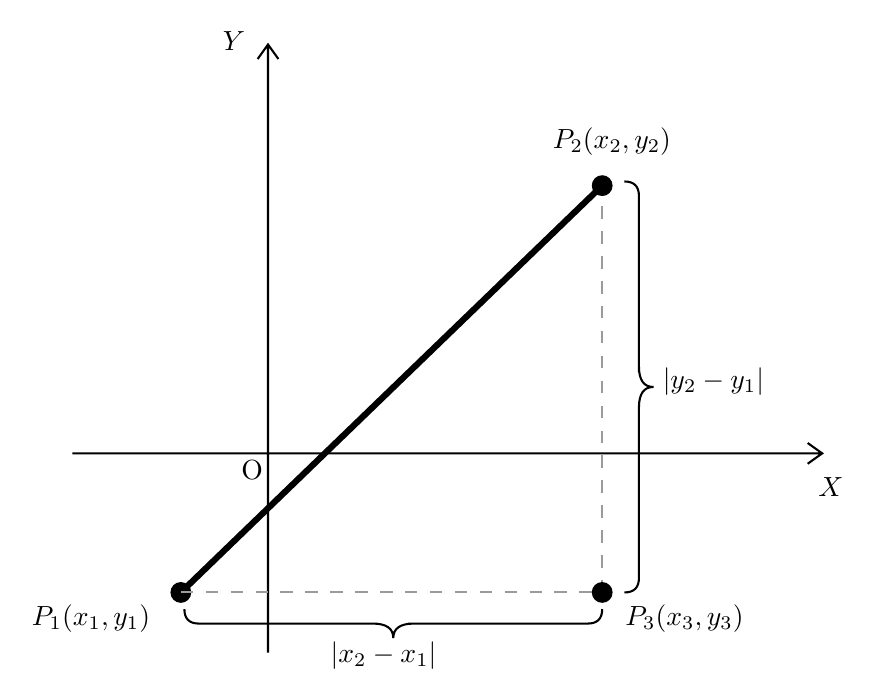
\begin{tikzpicture}[x=0.75pt,y=0.75pt,yscale=-1,xscale=1]
		%uncomment if require: \path (0,771); %set diagram left start at 0, and has height of 771
		
		%Straight Lines [id:da2415553186763082] 
		\draw [color={rgb, 255:red, 155; green, 155; blue, 155 }  ,draw opacity=1 ] [dash pattern={on 4.5pt off 4.5pt}]  (386.3,303) -- (386.3,107) ;
		%Shape: Axis 2D [id:dp5152191739484895] 
		\draw  (131,236) -- (492.3,236)(225.3,39) -- (225.3,332) (485.3,231) -- (492.3,236) -- (485.3,241) (220.3,46) -- (225.3,39) -- (230.3,46)  ;
		%Straight Lines [id:da569264291027562] 
		\draw [line width=2.25]    (183.3,303) -- (386.3,107) ;
		%Shape: Circle [id:dp19445824712476356] 
		\draw  [fill={rgb, 255:red, 0; green, 0; blue, 0 }  ,fill opacity=1 ] (381.8,107) .. controls (381.8,104.51) and (383.81,102.5) .. (386.3,102.5) .. controls (388.79,102.5) and (390.8,104.51) .. (390.8,107) .. controls (390.8,109.49) and (388.79,111.5) .. (386.3,111.5) .. controls (383.81,111.5) and (381.8,109.49) .. (381.8,107) -- cycle ;
		%Shape: Circle [id:dp8103691548157195] 
		\draw  [fill={rgb, 255:red, 0; green, 0; blue, 0 }  ,fill opacity=1 ] (178.8,303) .. controls (178.8,300.51) and (180.81,298.5) .. (183.3,298.5) .. controls (185.79,298.5) and (187.8,300.51) .. (187.8,303) .. controls (187.8,305.49) and (185.79,307.5) .. (183.3,307.5) .. controls (180.81,307.5) and (178.8,305.49) .. (178.8,303) -- cycle ;
		%Straight Lines [id:da45404450758217707] 
		\draw [color={rgb, 255:red, 155; green, 155; blue, 155 }  ,draw opacity=1 ] [dash pattern={on 4.5pt off 4.5pt}]  (183.3,303) -- (386.3,303) ;
		%Shape: Circle [id:dp5479521029696481] 
		\draw  [fill={rgb, 255:red, 0; green, 0; blue, 0 }  ,fill opacity=1 ] (381.8,303) .. controls (381.8,300.51) and (383.81,298.5) .. (386.3,298.5) .. controls (388.79,298.5) and (390.8,300.51) .. (390.8,303) .. controls (390.8,305.49) and (388.79,307.5) .. (386.3,307.5) .. controls (383.81,307.5) and (381.8,305.49) .. (381.8,303) -- cycle ;
		%Shape: Brace [id:dp4014584698158996] 
		\draw   (185,311) .. controls (185,315.67) and (187.33,318) .. (192,318) -- (275.65,318) .. controls (282.32,318) and (285.65,320.33) .. (285.65,325) .. controls (285.65,320.33) and (288.98,318) .. (295.65,318)(292.65,318) -- (379.3,318) .. controls (383.97,318) and (386.3,315.67) .. (386.3,311) ;
		%Shape: Brace [id:dp46199612063032447] 
		\draw   (397,303) .. controls (401.67,303) and (404,300.67) .. (404,296) -- (404,214) .. controls (404,207.33) and (406.33,204) .. (411,204) .. controls (406.33,204) and (404,200.67) .. (404,194)(404,197) -- (404,112) .. controls (404,107.33) and (401.67,105) .. (397,105) ;
		
		% Text Node
		\draw (202,31.4) node [anchor=north west][inner sep=0.75pt]    {$Y$};
		% Text Node
		\draw (489,246.4) node [anchor=north west][inner sep=0.75pt]    {$X$};
		% Text Node
		\draw (211,238) node [anchor=north west][inner sep=0.75pt]   [align=left] {O};
		% Text Node
		\draw (361,77.4) node [anchor=north west][inner sep=0.75pt]    {$P_{2}( x_{2} ,y_{2})$};
		% Text Node
		\draw (110,307.4) node [anchor=north west][inner sep=0.75pt]    {$P_{1}( x_{1} ,y_{1})$};
		% Text Node
		\draw (396,307.4) node [anchor=north west][inner sep=0.75pt]    {$P_{3}( x_{3} ,y_{3})$};
		% Text Node
		\draw (414,193.4) node [anchor=north west][inner sep=0.75pt]    {$| y_{2} -y_{1}| $};
		% Text Node
		\draw (254,325.4) node [anchor=north west][inner sep=0.75pt]    {$| x_{2} -x_{1}| $};
		\end{tikzpicture}
		\vspace*{3mm}
		\caption{Scenario of thee points in a plane}
	\end{figure}
	
	We can consider the straight line $\overline{P_1P_2}$ as a vector but not translated at the origin $\text{O}$ of the referential.
	
	If $x_1\neq x_2$ and $y_1\neq y_2$ (as in the figure above), the points $P_1,P_2,P_3$ are the vertices of a perpendicular triangle. By applying the Pythagorean theorem (\SeeChapter{see section Euclidean Geometry page \pageref{pythagorean theorem}}) we can easily calculate the metric distance $d$ between the points $P_1$ and $P_2$ as being equal to:
	
	On the figure, we see that:
	
	Since $\forall x \in \mathbb{R} \; \vert x \vert ^2 =x^2$, we can write:
	
	If $x_1=y_1=0$, we end up with a relation named "\NewTerm{norm}", "\NewTerm{module}" or "\NewTerm{distance}\index{distance}" that we have already defined as part of our study of Vector Calculus when the origin of the vector is translated on the origin of the referential (see section of the corresponding name page \pageref{vector norm}):
	
	\begin{theorem}
	Obviously, if we consider two points $P_1(x_1,y_1),P_2(x_2,y_2)$, we can determine if a third point $P_3(x_3,y_3)$ is on the mediator (\SeeChapter{see section Euclidean Geometry page \pageref{mediator}}) of the first two and for this that it is obviously sufficient that (by definition of the mediator!):
	
	\end{theorem}
	\begin{tcolorbox}[title=Remark,arc=10pt,breakable,drop lifted shadow,
  skin=enhanced,
  skin first is subskin of={enhancedfirst}{arc=10pt,no shadow},
  skin middle is subskin of={enhancedmiddle}{arc=10pt,no shadow},
  skin last is subskin of={enhancedlast}{drop lifted shadow}]
	We hesitated to put this proof in the section of Analytical Geometry but at then end we have decided that it was a nice example of showing how visual representation can help readers to better understand some subjects.
	\end{tcolorbox}	
	\begin{dem}
	As $(x_1,y_1),(x_2,y_2)$ are known, we can easily express an "\NewTerm{analytic expression}" property of the mediator\label{mediator analytic expression} that is that for each point on the mediator we have:
	
	where $a, b$ are therefore constants and wherein any point that satisfies this relation, which is in this case the equation of a straight line, lies on the mediator.
	\begin{flushright}
		$\blacksquare$  Q.E.D.
	\end{flushright}
	\end{dem}
	Furthermore, it is easy to see that the midpoint of the line segment that coincide with the mediator is given by:
	
	So we see that with a simple visual representation, we can achieve results that are sometimes (...) more obvious for students.
	
	Let us use this example to define some concepts on that we will come back further and do some reminders.
	
	\textbf{Definition (\#\thesection.\mydef):} Any function of the form of a polynomial (\SeeChapter{see section Calculus page \pageref{polynomial}}) of degree $1$ with constant real coefficients:
	
	is the analytic expression of what we name a "\NewTerm{straight line}\index{straight line}\label{straight line}" or "\NewTerm{linear equation}\index{linear equation}" of "\NewTerm{slope}\index{slope}" $a$ and "\NewTerm{intercept}\index{intercept}" $b$ (when $x=0$).
	
	Obviously, if:
	
	the line is horizontal if we graphically represent it since $y$ is constant for all $x$ and is equal to $b$. Conversely, if:
	
	the straight line will be vertical in the $x\text{O}y$ referential.
	
	\paragraph{Properties of visual representations}\mbox{}\\\\
	Depending on the type of graph we visualize (especially graphics planes) it is possible to extract some basic properties. Let us see the most important one to know for univariate functions:
	
	\begin{enumerate}
		\item[P1.] The graph of a function is "\NewTerm{symmetrical about the $y$-axis}\index{graph symmetric about the $y$-axis}" if the change in from $x$ to $-x$ in the function does not change the value of $y$ such that:
		\begin{figure}[H]
			\centering
			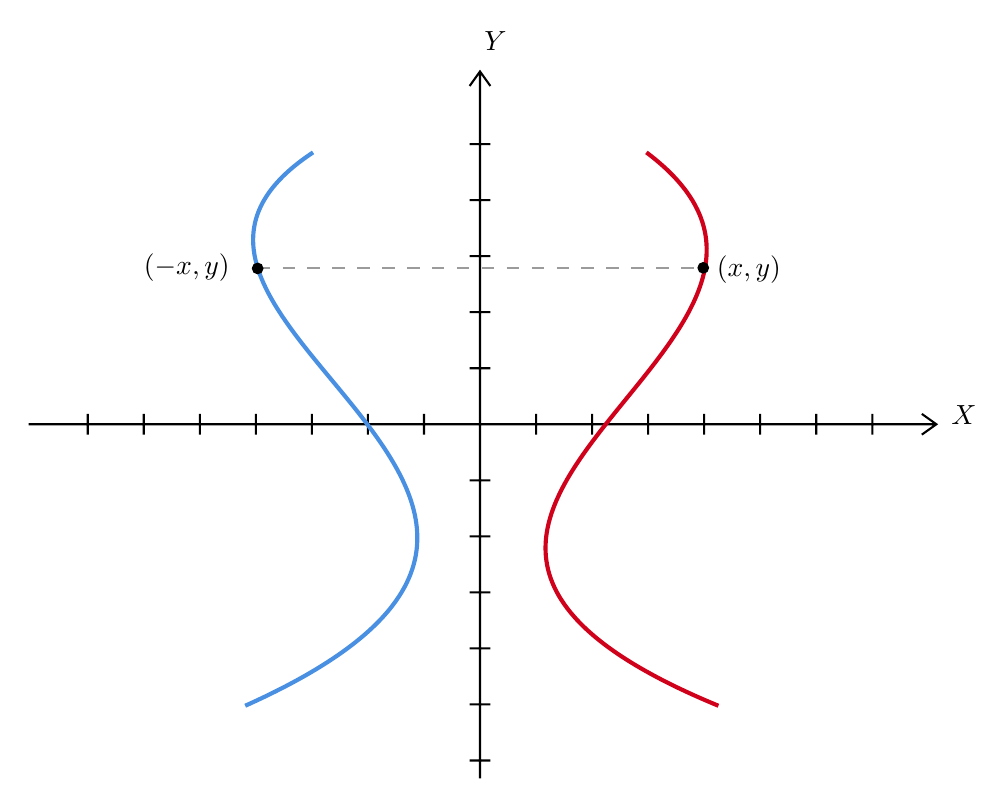
\begin{tikzpicture}[x=0.75pt,y=0.75pt,yscale=-1,xscale=1]
			%uncomment if require: \path (0,771); %set diagram left start at 0, and has height of 771
			
			%Shape: Axis 2D [id:dp7636403352579628] 
			\draw  (68,220.97) -- (505.3,220.97)(285.43,51) -- (285.43,391.6) (498.3,215.97) -- (505.3,220.97) -- (498.3,225.97) (280.43,58) -- (285.43,51) -- (290.43,58) (312.43,215.97) -- (312.43,225.97)(339.43,215.97) -- (339.43,225.97)(366.43,215.97) -- (366.43,225.97)(393.43,215.97) -- (393.43,225.97)(420.43,215.97) -- (420.43,225.97)(447.43,215.97) -- (447.43,225.97)(474.43,215.97) -- (474.43,225.97)(258.43,215.97) -- (258.43,225.97)(231.43,215.97) -- (231.43,225.97)(204.43,215.97) -- (204.43,225.97)(177.43,215.97) -- (177.43,225.97)(150.43,215.97) -- (150.43,225.97)(123.43,215.97) -- (123.43,225.97)(96.43,215.97) -- (96.43,225.97)(280.43,193.97) -- (290.43,193.97)(280.43,166.97) -- (290.43,166.97)(280.43,139.97) -- (290.43,139.97)(280.43,112.97) -- (290.43,112.97)(280.43,85.97) -- (290.43,85.97)(280.43,247.97) -- (290.43,247.97)(280.43,274.97) -- (290.43,274.97)(280.43,301.97) -- (290.43,301.97)(280.43,328.97) -- (290.43,328.97)(280.43,355.97) -- (290.43,355.97)(280.43,382.97) -- (290.43,382.97) ;
			\draw   ;
			%Curve Lines [id:da7098043564145642] 
			\draw [color={rgb, 255:red, 74; green, 144; blue, 226 }  ,draw opacity=1 ][line width=1.5]    (172.3,356.6) .. controls (395.3,256.6) and (84.3,169.6) .. (205,90) ;
			%Curve Lines [id:da31688466428341844] 
			\draw [color={rgb, 255:red, 208; green, 2; blue, 27 }  ,draw opacity=1 ][line width=1.5]    (400.3,356.6) .. controls (177.3,264.6) and (486.3,180.6) .. (365.6,90) ;
			%Straight Lines [id:da5040595412454372] 
			\draw [color={rgb, 255:red, 155; green, 155; blue, 155 }  ,draw opacity=1 ] [dash pattern={on 4.5pt off 4.5pt}]  (178.3,145.6) -- (395.3,145.6) ;
			%Shape: Circle [id:dp21608464408795736] 
			\draw  [fill={rgb, 255:red, 0; green, 0; blue, 0 }  ,fill opacity=1 ] (176,145.9) .. controls (176,144.63) and (177.03,143.6) .. (178.3,143.6) .. controls (179.57,143.6) and (180.6,144.63) .. (180.6,145.9) .. controls (180.6,147.17) and (179.57,148.2) .. (178.3,148.2) .. controls (177.03,148.2) and (176,147.17) .. (176,145.9) -- cycle ;
			%Shape: Circle [id:dp17037014344743073] 
			\draw  [fill={rgb, 255:red, 0; green, 0; blue, 0 }  ,fill opacity=1 ] (390.7,145.6) .. controls (390.7,144.33) and (391.73,143.3) .. (393,143.3) .. controls (394.27,143.3) and (395.3,144.33) .. (395.3,145.6) .. controls (395.3,146.87) and (394.27,147.9) .. (393,147.9) .. controls (391.73,147.9) and (390.7,146.87) .. (390.7,145.6) -- cycle ;
			
			% Text Node
			\draw (286,30.4) node [anchor=north west][inner sep=0.75pt]    {$Y$};
			% Text Node
			\draw (511,210.4) node [anchor=north west][inner sep=0.75pt]    {$X$};
			% Text Node
			\draw (122,137.4) node [anchor=north west][inner sep=0.75pt]    {$( -x,y)$};
			% Text Node
			\draw (398,138.4) node [anchor=north west][inner sep=0.75pt]    {$( x,y)$};
			\end{tikzpicture}
			\vspace*{3mm}
			\caption{Example of symmetry through the $y$-axis of a function}
		\end{figure}
		
		\item[P2.] The graph of a function is "\NewTerm{symmetrical about the $x$-axis}\index{graph symmetric about the $x$-axis}" if the change from $y$ to $-y$ does not change the value of $x$ such that:
		\begin{figure}[H]
			\centering
			\begin{tikzpicture}[x=0.75pt,y=0.75pt,yscale=-1,xscale=1]
			%uncomment if require: \path (0,771); %set diagram left start at 0, and has height of 771
			
			%Shape: Axis 2D [id:dp7636403352579628] 
			\draw  (64,220.97) -- (501.3,220.97)(281.43,51) -- (281.43,391.6) (494.3,215.97) -- (501.3,220.97) -- (494.3,225.97) (276.43,58) -- (281.43,51) -- (286.43,58) (307.43,215.97) -- (307.43,225.97)(333.43,215.97) -- (333.43,225.97)(359.43,215.97) -- (359.43,225.97)(385.43,215.97) -- (385.43,225.97)(411.43,215.97) -- (411.43,225.97)(437.43,215.97) -- (437.43,225.97)(463.43,215.97) -- (463.43,225.97)(255.43,215.97) -- (255.43,225.97)(229.43,215.97) -- (229.43,225.97)(203.43,215.97) -- (203.43,225.97)(177.43,215.97) -- (177.43,225.97)(151.43,215.97) -- (151.43,225.97)(125.43,215.97) -- (125.43,225.97)(99.43,215.97) -- (99.43,225.97)(73.43,215.97) -- (73.43,225.97)(276.43,194.97) -- (286.43,194.97)(276.43,168.97) -- (286.43,168.97)(276.43,142.97) -- (286.43,142.97)(276.43,116.97) -- (286.43,116.97)(276.43,90.97) -- (286.43,90.97)(276.43,246.97) -- (286.43,246.97)(276.43,272.97) -- (286.43,272.97)(276.43,298.97) -- (286.43,298.97)(276.43,324.97) -- (286.43,324.97)(276.43,350.97) -- (286.43,350.97)(276.43,376.97) -- (286.43,376.97) ;
			\draw   ;
			%Curve Lines [id:da4704859139391653] 
			\draw [color={rgb, 255:red, 208; green, 2; blue, 27 }  ,draw opacity=1 ][line width=1.5]    (147.3,144.6) .. controls (205.3,309.6) and (360.3,59.6) .. (417.3,176.6) ;
			%Curve Lines [id:da11697100961495077] 
			\draw [color={rgb, 255:red, 74; green, 144; blue, 226 }  ,draw opacity=1 ][line width=1.5]    (150.3,299.6) .. controls (193.3,128.6) and (360.3,381.6) .. (416.3,267.6) ;
			%Straight Lines [id:da24527238675948082] 
			\draw [color={rgb, 255:red, 155; green, 155; blue, 155 }  ,draw opacity=1 ] [dash pattern={on 4.5pt off 4.5pt}]  (372,144) -- (372,295.6) ;
			%Shape: Circle [id:dp4802337367009828] 
			\draw  [fill={rgb, 255:red, 0; green, 0; blue, 0 }  ,fill opacity=1 ] (369.65,144.35) .. controls (369.65,143.05) and (370.7,142) .. (372,142) .. controls (373.3,142) and (374.35,143.05) .. (374.35,144.35) .. controls (374.35,145.65) and (373.3,146.7) .. (372,146.7) .. controls (370.7,146.7) and (369.65,145.65) .. (369.65,144.35) -- cycle ;
			%Shape: Circle [id:dp9289403234164584] 
			\draw  [fill={rgb, 255:red, 0; green, 0; blue, 0 }  ,fill opacity=1 ] (369.65,297.6) .. controls (369.65,296.3) and (370.7,295.25) .. (372,295.25) .. controls (373.3,295.25) and (374.35,296.3) .. (374.35,297.6) .. controls (374.35,298.9) and (373.3,299.95) .. (372,299.95) .. controls (370.7,299.95) and (369.65,298.9) .. (369.65,297.6) -- cycle ;
			
			% Text Node
			\draw (286,30.4) node [anchor=north west][inner sep=0.75pt]    {$Y$};
			% Text Node
			\draw (511,210.4) node [anchor=north west][inner sep=0.75pt]    {$X$};
			% Text Node
			\draw (355,119.4) node [anchor=north west][inner sep=0.75pt]    {$( x,y)$};
			% Text Node
			\draw (349,305.4) node [anchor=north west][inner sep=0.75pt]    {$( -x,y)$};
			\end{tikzpicture}
			\vspace*{3mm}
			\caption{Example of symmetry through the $x$-axis of a function}
		\end{figure}
		
		\item[P3.] The graph of a function is "\NewTerm{symmetrical about the origin $\text{O}$}\index{graph symmetrical about the origin}" if the simultaneous change of $y$ to $-y$ and from $x$ to $-x$ gives the following result (that is to say that the change in the sign of one variable change the sign of the other):
		\begin{figure}[H]
			\centering
			\begin{tikzpicture}[x=0.75pt,y=0.75pt,yscale=-1,xscale=1]
			%uncomment if require: \path (0,771); %set diagram left start at 0, and has height of 771
			
			%Shape: Axis 2D [id:dp7636403352579628] 
			\draw  (64,220.97) -- (501.3,220.97)(281.43,51) -- (281.43,391.6) (494.3,215.97) -- (501.3,220.97) -- (494.3,225.97) (276.43,58) -- (281.43,51) -- (286.43,58) (307.43,215.97) -- (307.43,225.97)(333.43,215.97) -- (333.43,225.97)(359.43,215.97) -- (359.43,225.97)(385.43,215.97) -- (385.43,225.97)(411.43,215.97) -- (411.43,225.97)(437.43,215.97) -- (437.43,225.97)(463.43,215.97) -- (463.43,225.97)(255.43,215.97) -- (255.43,225.97)(229.43,215.97) -- (229.43,225.97)(203.43,215.97) -- (203.43,225.97)(177.43,215.97) -- (177.43,225.97)(151.43,215.97) -- (151.43,225.97)(125.43,215.97) -- (125.43,225.97)(99.43,215.97) -- (99.43,225.97)(73.43,215.97) -- (73.43,225.97)(276.43,194.97) -- (286.43,194.97)(276.43,168.97) -- (286.43,168.97)(276.43,142.97) -- (286.43,142.97)(276.43,116.97) -- (286.43,116.97)(276.43,90.97) -- (286.43,90.97)(276.43,246.97) -- (286.43,246.97)(276.43,272.97) -- (286.43,272.97)(276.43,298.97) -- (286.43,298.97)(276.43,324.97) -- (286.43,324.97)(276.43,350.97) -- (286.43,350.97)(276.43,376.97) -- (286.43,376.97) ;
			\draw   ;
			%Curve Lines [id:da7098043564145642] 
			\draw [color={rgb, 255:red, 74; green, 144; blue, 226 }  ,draw opacity=1 ][line width=1.5]    (180.3,350.6) .. controls (403.3,250.6) and (4.6,319.2) .. (125.3,239.6) ;
			%Curve Lines [id:da31688466428341844] 
			\draw [color={rgb, 255:red, 208; green, 2; blue, 27 }  ,draw opacity=1 ][line width=1.5]    (437.3,200.6) .. controls (547.3,123.6) and (162.3,188.6) .. (381.3,90.6) ;
			%Straight Lines [id:da5040595412454372] 
			\draw [color={rgb, 255:red, 155; green, 155; blue, 155 }  ,draw opacity=1 ] [dash pattern={on 4.5pt off 4.5pt}]  (249.3,302.6) -- (312.3,136.6) ;
			%Shape: Circle [id:dp21608464408795736] 
			\draw  [fill={rgb, 255:red, 0; green, 0; blue, 0 }  ,fill opacity=1 ] (247.3,302.6) .. controls (247.3,301.33) and (248.33,300.3) .. (249.6,300.3) .. controls (250.87,300.3) and (251.9,301.33) .. (251.9,302.6) .. controls (251.9,303.87) and (250.87,304.9) .. (249.6,304.9) .. controls (248.33,304.9) and (247.3,303.87) .. (247.3,302.6) -- cycle ;
			%Shape: Circle [id:dp17037014344743073] 
			\draw  [fill={rgb, 255:red, 0; green, 0; blue, 0 }  ,fill opacity=1 ] (310,136.6) .. controls (310,135.33) and (311.03,134.3) .. (312.3,134.3) .. controls (313.57,134.3) and (314.6,135.33) .. (314.6,136.6) .. controls (314.6,137.87) and (313.57,138.9) .. (312.3,138.9) .. controls (311.03,138.9) and (310,137.87) .. (310,136.6) -- cycle ;
			
			% Text Node
			\draw (286,30.4) node [anchor=north west][inner sep=0.75pt]    {$Y$};
			% Text Node
			\draw (511,210.4) node [anchor=north west][inner sep=0.75pt]    {$X$};
			% Text Node
			\draw (181,297.4) node [anchor=north west][inner sep=0.75pt]    {$( -x,-y)$};
			% Text Node
			\draw (321,123.4) node [anchor=north west][inner sep=0.75pt]    {$( x,y)$};
			\end{tikzpicture}
			\vspace*{3mm}
			\caption{Example of symmetry through the origin $\text{O}$ of a function}
		\end{figure}
		
		\item[P4.] Given a function $y=f(x)$, if we add a constant $c^{te} \geq 0$ to this function as:
		
		then the function $f(x)$ is shifted (or "translated") vertically upwards of a distance $c^{te}$ as presented in the figure below:
		\begin{figure}[H]
			\centering
			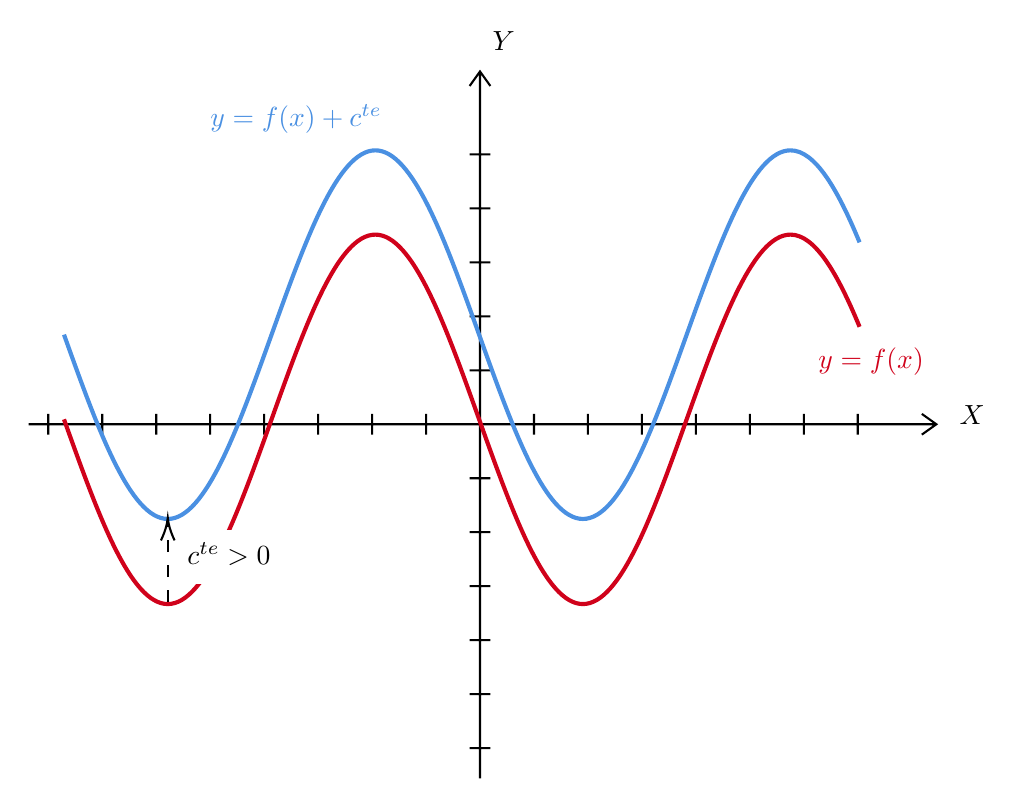
\begin{tikzpicture}[x=0.75pt,y=0.75pt,yscale=-1,xscale=1]
			%uncomment if require: \path (0,771); %set diagram left start at 0, and has height of 771
			
			%Shape: Axis 2D [id:dp7636403352579628] 
			\draw  (64,220.97) -- (501.3,220.97)(281.43,51) -- (281.43,391.6) (494.3,215.97) -- (501.3,220.97) -- (494.3,225.97) (276.43,58) -- (281.43,51) -- (286.43,58) (307.43,215.97) -- (307.43,225.97)(333.43,215.97) -- (333.43,225.97)(359.43,215.97) -- (359.43,225.97)(385.43,215.97) -- (385.43,225.97)(411.43,215.97) -- (411.43,225.97)(437.43,215.97) -- (437.43,225.97)(463.43,215.97) -- (463.43,225.97)(255.43,215.97) -- (255.43,225.97)(229.43,215.97) -- (229.43,225.97)(203.43,215.97) -- (203.43,225.97)(177.43,215.97) -- (177.43,225.97)(151.43,215.97) -- (151.43,225.97)(125.43,215.97) -- (125.43,225.97)(99.43,215.97) -- (99.43,225.97)(73.43,215.97) -- (73.43,225.97)(276.43,194.97) -- (286.43,194.97)(276.43,168.97) -- (286.43,168.97)(276.43,142.97) -- (286.43,142.97)(276.43,116.97) -- (286.43,116.97)(276.43,90.97) -- (286.43,90.97)(276.43,246.97) -- (286.43,246.97)(276.43,272.97) -- (286.43,272.97)(276.43,298.97) -- (286.43,298.97)(276.43,324.97) -- (286.43,324.97)(276.43,350.97) -- (286.43,350.97)(276.43,376.97) -- (286.43,376.97) ;
			\draw   ;
			%Shape: Wave [id:dp935589976697009] 
			\draw  [color={rgb, 255:red, 74; green, 144; blue, 226 }  ,draw opacity=1 ][line width=1.5]  (81,177.8) .. controls (97.31,223.29) and (112.9,266.6) .. (131,266.6) .. controls (149.1,266.6) and (164.69,223.29) .. (181,177.8) .. controls (197.31,132.31) and (212.9,89) .. (231,89) .. controls (249.1,89) and (264.69,132.31) .. (281,177.8) .. controls (297.31,223.29) and (312.9,266.6) .. (331,266.6) .. controls (349.1,266.6) and (364.69,223.29) .. (381,177.8) .. controls (397.31,132.31) and (412.9,89) .. (431,89) .. controls (442.87,89) and (453.67,107.65) .. (464.3,133.32) ;
			%Shape: Wave [id:dp7617198593557306] 
			\draw  [color={rgb, 255:red, 208; green, 2; blue, 27 }  ,draw opacity=1 ][line width=1.5]  (81,218.6) .. controls (97.31,264.19) and (112.9,307.6) .. (131,307.6) .. controls (149.1,307.6) and (164.69,264.19) .. (181,218.6) .. controls (197.31,173.01) and (212.9,129.6) .. (231,129.6) .. controls (249.1,129.6) and (264.69,173.01) .. (281,218.6) .. controls (297.31,264.19) and (312.9,307.6) .. (331,307.6) .. controls (349.1,307.6) and (364.69,264.19) .. (381,218.6) .. controls (397.31,173.01) and (412.9,129.6) .. (431,129.6) .. controls (442.87,129.6) and (453.67,148.29) .. (464.3,174.02) ;
			%Straight Lines [id:da05213646593625976] 
			\draw  [dash pattern={on 4.5pt off 4.5pt}]  (131,306.6) -- (131,268) ;
			\draw [shift={(131,266)}, rotate = 90] [color={rgb, 255:red, 0; green, 0; blue, 0 }  ][line width=0.75]    (10.93,-3.29) .. controls (6.95,-1.4) and (3.31,-0.3) .. (0,0) .. controls (3.31,0.3) and (6.95,1.4) .. (10.93,3.29)   ;
			
			% Text Node
			\draw (286,30.4) node [anchor=north west][inner sep=0.75pt]    {$Y$};
			% Text Node
			\draw (511,210.4) node [anchor=north west][inner sep=0.75pt]    {$X$};
			% Text Node
			\draw (443,182.4) node [anchor=north west][inner sep=0.75pt]  [color={rgb, 255:red, 208; green, 2; blue, 27 }  ,opacity=1 ]  {$y=f( x)$};
			% Text Node
			\draw (150,65.4) node [anchor=north west][inner sep=0.75pt]  [color={rgb, 255:red, 74; green, 144; blue, 226 }  ,opacity=1 ]  {$y=f( x) +c^{te}$};
			% Text Node
			\draw  [draw opacity=0][fill={rgb, 255:red, 255; green, 255; blue, 255 }  ,fill opacity=1 ]  (136,272) -- (192,272) -- (192,298) -- (136,298) -- cycle  ;
			\draw (139,276.4) node [anchor=north west][inner sep=0.75pt]    {$c^{te}  >0$};
			\end{tikzpicture}
			\vspace*{3mm}
			\caption{Example of a positive vertical translation of a function}
		\end{figure}
		And conversely if $c^{te} \geq 0$ but:
		
		then the function $f(x)$  is obviously translated vertically downwards:
		\begin{figure}[H]
			\centering
			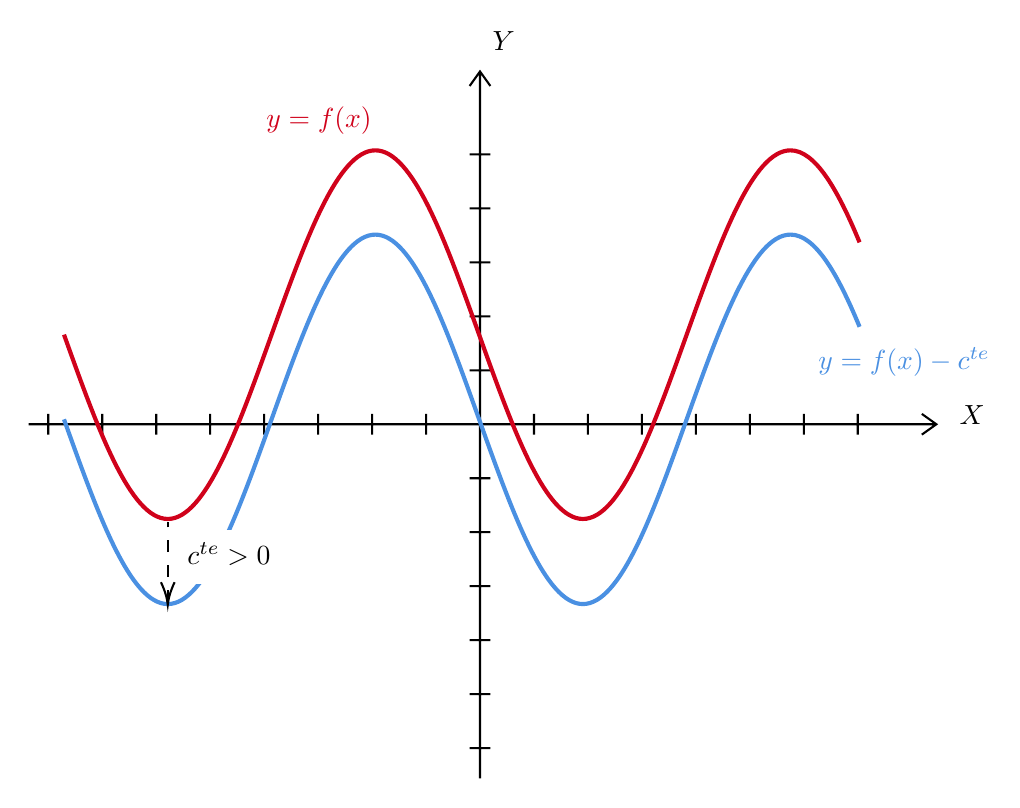
\begin{tikzpicture}[x=0.75pt,y=0.75pt,yscale=-1,xscale=1]
			%uncomment if require: \path (0,771); %set diagram left start at 0, and has height of 771
			
			%Shape: Axis 2D [id:dp7636403352579628] 
			\draw  (64,220.97) -- (501.3,220.97)(281.43,51) -- (281.43,391.6) (494.3,215.97) -- (501.3,220.97) -- (494.3,225.97) (276.43,58) -- (281.43,51) -- (286.43,58) (307.43,215.97) -- (307.43,225.97)(333.43,215.97) -- (333.43,225.97)(359.43,215.97) -- (359.43,225.97)(385.43,215.97) -- (385.43,225.97)(411.43,215.97) -- (411.43,225.97)(437.43,215.97) -- (437.43,225.97)(463.43,215.97) -- (463.43,225.97)(255.43,215.97) -- (255.43,225.97)(229.43,215.97) -- (229.43,225.97)(203.43,215.97) -- (203.43,225.97)(177.43,215.97) -- (177.43,225.97)(151.43,215.97) -- (151.43,225.97)(125.43,215.97) -- (125.43,225.97)(99.43,215.97) -- (99.43,225.97)(73.43,215.97) -- (73.43,225.97)(276.43,194.97) -- (286.43,194.97)(276.43,168.97) -- (286.43,168.97)(276.43,142.97) -- (286.43,142.97)(276.43,116.97) -- (286.43,116.97)(276.43,90.97) -- (286.43,90.97)(276.43,246.97) -- (286.43,246.97)(276.43,272.97) -- (286.43,272.97)(276.43,298.97) -- (286.43,298.97)(276.43,324.97) -- (286.43,324.97)(276.43,350.97) -- (286.43,350.97)(276.43,376.97) -- (286.43,376.97) ;
			\draw   ;
			%Shape: Wave [id:dp935589976697009] 
			\draw  [color={rgb, 255:red, 208; green, 2; blue, 27 }  ,draw opacity=1 ][line width=1.5]  (81,177.8) .. controls (97.31,223.29) and (112.9,266.6) .. (131,266.6) .. controls (149.1,266.6) and (164.69,223.29) .. (181,177.8) .. controls (197.31,132.31) and (212.9,89) .. (231,89) .. controls (249.1,89) and (264.69,132.31) .. (281,177.8) .. controls (297.31,223.29) and (312.9,266.6) .. (331,266.6) .. controls (349.1,266.6) and (364.69,223.29) .. (381,177.8) .. controls (397.31,132.31) and (412.9,89) .. (431,89) .. controls (442.87,89) and (453.67,107.65) .. (464.3,133.32) ;
			%Shape: Wave [id:dp7617198593557306] 
			\draw  [color={rgb, 255:red, 74; green, 144; blue, 226 }  ,draw opacity=1 ][line width=1.5]  (81,218.6) .. controls (97.31,264.19) and (112.9,307.6) .. (131,307.6) .. controls (149.1,307.6) and (164.69,264.19) .. (181,218.6) .. controls (197.31,173.01) and (212.9,129.6) .. (231,129.6) .. controls (249.1,129.6) and (264.69,173.01) .. (281,218.6) .. controls (297.31,264.19) and (312.9,307.6) .. (331,307.6) .. controls (349.1,307.6) and (364.69,264.19) .. (381,218.6) .. controls (397.31,173.01) and (412.9,129.6) .. (431,129.6) .. controls (442.87,129.6) and (453.67,148.29) .. (464.3,174.02) ;
			
			%Straight Lines [id:da7399340167307238] 
		\draw  [dash pattern={on 4.5pt off 4.5pt}]  (131,306.6) -- (131,268) ;
		\draw [shift={(131,308)}, rotate = 270] [color={rgb, 255:red, 0; green, 0; blue, 0 }  ][line width=0.75]    (10.93,-3.29) .. controls (6.95,-1.4) and (3.31,-0.3) .. (0,0) .. controls (3.31,0.3) and (6.95,1.4) .. (10.93,3.29)   ;

			
			% Text Node
			\draw (286,30.4) node [anchor=north west][inner sep=0.75pt]    {$Y$};
			% Text Node
			\draw (511,210.4) node [anchor=north west][inner sep=0.75pt]    {$X$};
			% Text Node
			\draw (443,182.4) node [anchor=north west][inner sep=0.75pt]  [color={rgb, 255:red, 74; green, 144; blue, 226 }  ,opacity=1 ]  {$y=f( x) -c^{te}$};
			% Text Node
			\draw (177,66.4) node [anchor=north west][inner sep=0.75pt]  [color={rgb, 255:red, 208; green, 2; blue, 27 }  ,opacity=1 ]  {$y=f( x)$};
			% Text Node
			\draw  [draw opacity=0][fill={rgb, 255:red, 255; green, 255; blue, 255 }  ,fill opacity=1 ]  (136,272) -- (192,272) -- (192,298) -- (136,298) -- cycle  ;
			\draw (139,276.4) node [anchor=north west][inner sep=0.75pt]    {$c^{te}  >0$};
			\end{tikzpicture}
			\vspace*{3mm}
			\caption{Example of a negative vertical translation of a function}
		\end{figure}
		We can also consider horizontal translations of functions. Specifically, if we have still $c^{te}>0$, then $y=f(x)$ is translated horizontally to the right if we write:
		
		which graphically is represented by:
		\begin{figure}[H]
			\centering
			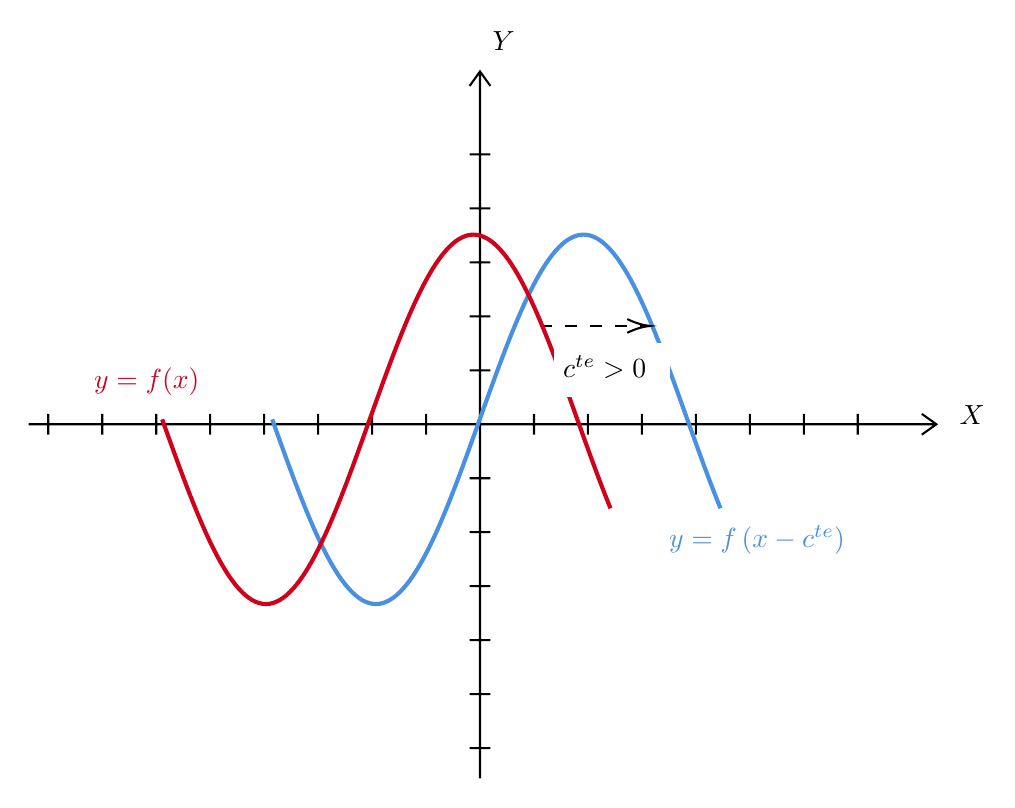
\begin{tikzpicture}[x=0.75pt,y=0.75pt,yscale=-1,xscale=1]
			%uncomment if require: \path (0,771); %set diagram left start at 0, and has height of 771
			
			%Shape: Axis 2D [id:dp7636403352579628] 
			\draw  (64,220.97) -- (501.3,220.97)(281.43,51) -- (281.43,391.6) (494.3,215.97) -- (501.3,220.97) -- (494.3,225.97) (276.43,58) -- (281.43,51) -- (286.43,58) (307.43,215.97) -- (307.43,225.97)(333.43,215.97) -- (333.43,225.97)(359.43,215.97) -- (359.43,225.97)(385.43,215.97) -- (385.43,225.97)(411.43,215.97) -- (411.43,225.97)(437.43,215.97) -- (437.43,225.97)(463.43,215.97) -- (463.43,225.97)(255.43,215.97) -- (255.43,225.97)(229.43,215.97) -- (229.43,225.97)(203.43,215.97) -- (203.43,225.97)(177.43,215.97) -- (177.43,225.97)(151.43,215.97) -- (151.43,225.97)(125.43,215.97) -- (125.43,225.97)(99.43,215.97) -- (99.43,225.97)(73.43,215.97) -- (73.43,225.97)(276.43,194.97) -- (286.43,194.97)(276.43,168.97) -- (286.43,168.97)(276.43,142.97) -- (286.43,142.97)(276.43,116.97) -- (286.43,116.97)(276.43,90.97) -- (286.43,90.97)(276.43,246.97) -- (286.43,246.97)(276.43,272.97) -- (286.43,272.97)(276.43,298.97) -- (286.43,298.97)(276.43,324.97) -- (286.43,324.97)(276.43,350.97) -- (286.43,350.97)(276.43,376.97) -- (286.43,376.97) ;
			\draw   ;
			%Shape: Wave [id:dp7617198593557306] 
			\draw  [color={rgb, 255:red, 74; green, 144; blue, 226 }  ,draw opacity=1 ][line width=1.5]  (181.3,218.6) .. controls (197.61,264.19) and (213.2,307.6) .. (231.3,307.6) .. controls (249.4,307.6) and (264.99,264.19) .. (281.3,218.6) .. controls (297.61,173.01) and (313.2,129.6) .. (331.3,129.6) .. controls (349.4,129.6) and (364.99,173.01) .. (381.3,218.6) .. controls (386.67,233.62) and (391.97,248.4) .. (397.3,261.47) ;
			%Straight Lines [id:da05213646593625976] 
			\draw  [dash pattern={on 4.5pt off 4.5pt}]  (310.3,173.6) -- (361.3,173.6) ;
			\draw [shift={(363.3,173.6)}, rotate = 180] [color={rgb, 255:red, 0; green, 0; blue, 0 }  ][line width=0.75]    (10.93,-3.29) .. controls (6.95,-1.4) and (3.31,-0.3) .. (0,0) .. controls (3.31,0.3) and (6.95,1.4) .. (10.93,3.29)   ;
			%Shape: Wave [id:dp9632619658707933] 
			\draw  [color={rgb, 255:red, 208; green, 2; blue, 27 }  ,draw opacity=1 ][line width=1.5]  (128.3,218.6) .. controls (144.61,264.19) and (160.2,307.6) .. (178.3,307.6) .. controls (196.4,307.6) and (211.99,264.19) .. (228.3,218.6) .. controls (244.61,173.01) and (260.2,129.6) .. (278.3,129.6) .. controls (296.4,129.6) and (311.99,173.01) .. (328.3,218.6) .. controls (333.67,233.62) and (338.97,248.4) .. (344.3,261.47) ;
			
			% Text Node
			\draw (286,30.4) node [anchor=north west][inner sep=0.75pt]    {$Y$};
			% Text Node
			\draw (511,210.4) node [anchor=north west][inner sep=0.75pt]    {$X$};
			% Text Node
			\draw (94,192.4) node [anchor=north west][inner sep=0.75pt]  [color={rgb, 255:red, 208; green, 2; blue, 27 }  ,opacity=1 ]  {$y=f( x)$};
			% Text Node
			\draw (371,268.4) node [anchor=north west][inner sep=0.75pt]  [color={rgb, 255:red, 74; green, 144; blue, 226 }  ,opacity=1 ]  {$y=f\left( x-c^{te}\right)$};
			% Text Node
			\draw  [draw opacity=0][fill={rgb, 255:red, 255; green, 255; blue, 255 }  ,fill opacity=1 ]  (317,182) -- (373,182) -- (373,208) -- (317,208) -- cycle  ;
			\draw (320,186.4) node [anchor=north west][inner sep=0.75pt]    {$c^{te}  >0$};
			\end{tikzpicture}
			\vspace*{3mm}
			\caption{Example of negative horizontal translation of a function}
		\end{figure}
		and conversely, translated horizontally to the left, if we write:
		
		as shown in the graph below:
		\begin{figure}[H]
			\centering
			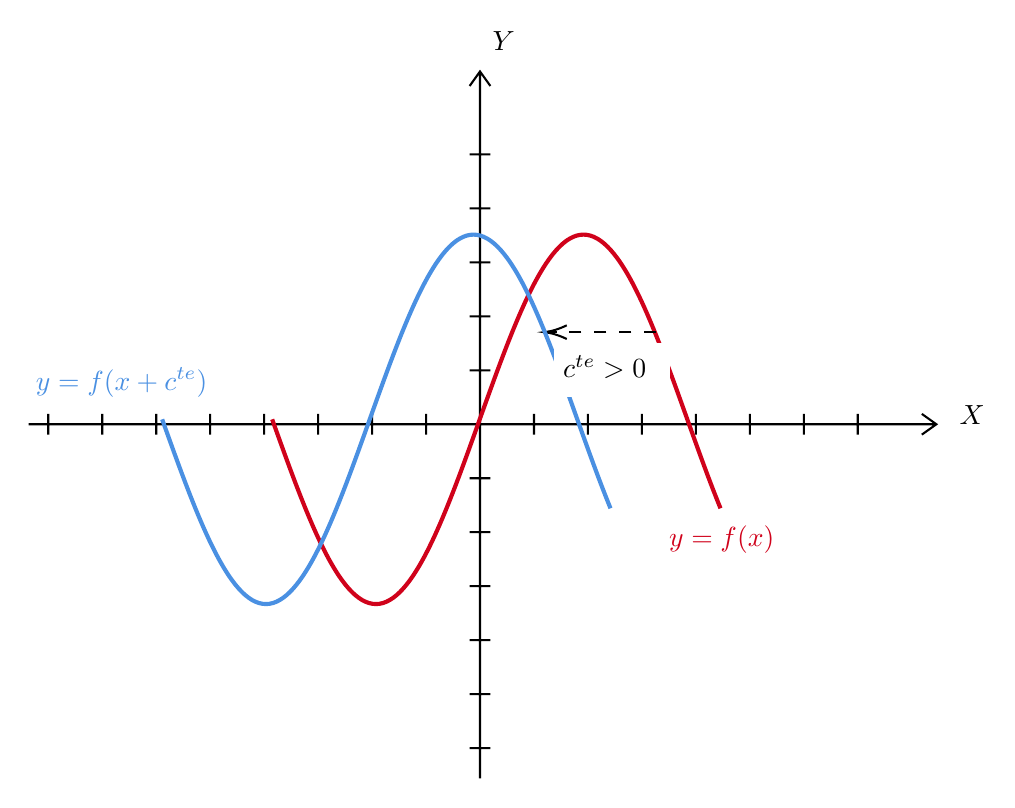
\begin{tikzpicture}[x=0.75pt,y=0.75pt,yscale=-1,xscale=1]
			%uncomment if require: \path (0,771); %set diagram left start at 0, and has height of 771
			
			%Shape: Axis 2D [id:dp7636403352579628] 
			\draw  (64,220.97) -- (501.3,220.97)(281.43,51) -- (281.43,391.6) (494.3,215.97) -- (501.3,220.97) -- (494.3,225.97) (276.43,58) -- (281.43,51) -- (286.43,58) (307.43,215.97) -- (307.43,225.97)(333.43,215.97) -- (333.43,225.97)(359.43,215.97) -- (359.43,225.97)(385.43,215.97) -- (385.43,225.97)(411.43,215.97) -- (411.43,225.97)(437.43,215.97) -- (437.43,225.97)(463.43,215.97) -- (463.43,225.97)(255.43,215.97) -- (255.43,225.97)(229.43,215.97) -- (229.43,225.97)(203.43,215.97) -- (203.43,225.97)(177.43,215.97) -- (177.43,225.97)(151.43,215.97) -- (151.43,225.97)(125.43,215.97) -- (125.43,225.97)(99.43,215.97) -- (99.43,225.97)(73.43,215.97) -- (73.43,225.97)(276.43,194.97) -- (286.43,194.97)(276.43,168.97) -- (286.43,168.97)(276.43,142.97) -- (286.43,142.97)(276.43,116.97) -- (286.43,116.97)(276.43,90.97) -- (286.43,90.97)(276.43,246.97) -- (286.43,246.97)(276.43,272.97) -- (286.43,272.97)(276.43,298.97) -- (286.43,298.97)(276.43,324.97) -- (286.43,324.97)(276.43,350.97) -- (286.43,350.97)(276.43,376.97) -- (286.43,376.97) ;
			\draw   ;
			%Shape: Wave [id:dp7617198593557306] 
			\draw  [color={rgb, 255:red, 208; green, 2; blue, 27 }  ,draw opacity=1 ][line width=1.5]  (181.3,218.6) .. controls (197.61,264.19) and (213.2,307.6) .. (231.3,307.6) .. controls (249.4,307.6) and (264.99,264.19) .. (281.3,218.6) .. controls (297.61,173.01) and (313.2,129.6) .. (331.3,129.6) .. controls (349.4,129.6) and (364.99,173.01) .. (381.3,218.6) .. controls (386.67,233.62) and (391.97,248.4) .. (397.3,261.47) ;
			%Straight Lines [id:da05213646593625976] 
			\draw  [dash pattern={on 4.5pt off 4.5pt}]  (366.3,176.6) -- (314.3,176.6) ;
			\draw [shift={(312.3,176.6)}, rotate = 360] [color={rgb, 255:red, 0; green, 0; blue, 0 }  ][line width=0.75]    (10.93,-3.29) .. controls (6.95,-1.4) and (3.31,-0.3) .. (0,0) .. controls (3.31,0.3) and (6.95,1.4) .. (10.93,3.29)   ;
			%Shape: Wave [id:dp9632619658707933] 
			\draw  [color={rgb, 255:red, 74; green, 144; blue, 226 }  ,draw opacity=1 ][line width=1.5]  (128.3,218.6) .. controls (144.61,264.19) and (160.2,307.6) .. (178.3,307.6) .. controls (196.4,307.6) and (211.99,264.19) .. (228.3,218.6) .. controls (244.61,173.01) and (260.2,129.6) .. (278.3,129.6) .. controls (296.4,129.6) and (311.99,173.01) .. (328.3,218.6) .. controls (333.67,233.62) and (338.97,248.4) .. (344.3,261.47) ;
			
			% Text Node
			\draw (286,30.4) node [anchor=north west][inner sep=0.75pt]    {$Y$};
			% Text Node
			\draw (511,210.4) node [anchor=north west][inner sep=0.75pt]    {$X$};
			% Text Node
			\draw (66,192.4) node [anchor=north west][inner sep=0.75pt]  [color={rgb, 255:red, 74; green, 144; blue, 226 }  ,opacity=1 ]  {$y=f(x+c^{te})$};
			% Text Node
			\draw (371,268.4) node [anchor=north west][inner sep=0.75pt]  [color={rgb, 255:red, 208; green, 2; blue, 27 }  ,opacity=1 ]  {$y=f( x)$};
			% Text Node
			\draw  [draw opacity=0][fill={rgb, 255:red, 255; green, 255; blue, 255 }  ,fill opacity=1 ]  (317,182) -- (373,182) -- (373,208) -- (317,208) -- cycle  ;
			\draw (320,186.4) node [anchor=north west][inner sep=0.75pt]    {$c^{te}  >0$};
			\end{tikzpicture}
			\vspace*{3mm}
			\caption{Example of positive horizontal translation of a function}
		\end{figure}
		To stretch or compress vertically a function, we simply multiply $y=f(x)$ by a constant $c^{te}>1$ and respectively $0\leq c^{te}<1$ as:
		
		and don't forget that if a function is linear then we have the special property $f(\lambda x)=\lambda f(x)$.
		
		This is graphically represented for the case $c^{te}>1$ by:
		\begin{figure}[H]
			\centering
			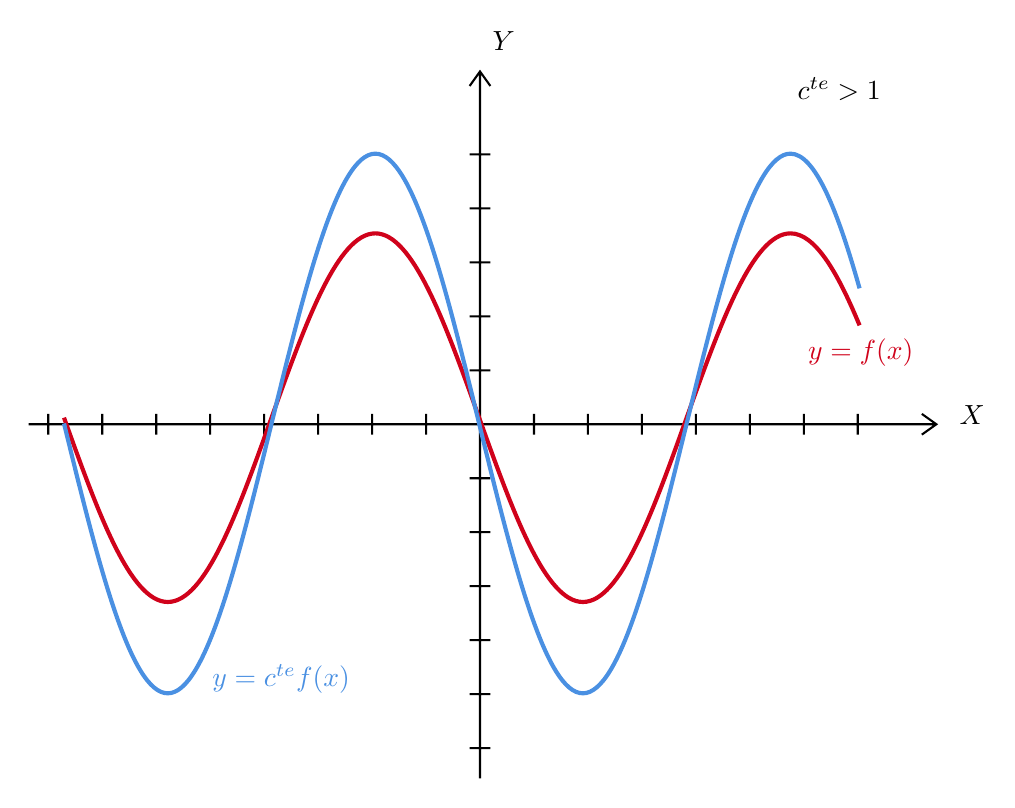
\begin{tikzpicture}[x=0.75pt,y=0.75pt,yscale=-1,xscale=1]
			%uncomment if require: \path (0,771); %set diagram left start at 0, and has height of 771
			
			%Shape: Axis 2D [id:dp7636403352579628] 
			\draw  (64,220.97) -- (501.3,220.97)(281.43,51) -- (281.43,391.6) (494.3,215.97) -- (501.3,220.97) -- (494.3,225.97) (276.43,58) -- (281.43,51) -- (286.43,58) (307.43,215.97) -- (307.43,225.97)(333.43,215.97) -- (333.43,225.97)(359.43,215.97) -- (359.43,225.97)(385.43,215.97) -- (385.43,225.97)(411.43,215.97) -- (411.43,225.97)(437.43,215.97) -- (437.43,225.97)(463.43,215.97) -- (463.43,225.97)(255.43,215.97) -- (255.43,225.97)(229.43,215.97) -- (229.43,225.97)(203.43,215.97) -- (203.43,225.97)(177.43,215.97) -- (177.43,225.97)(151.43,215.97) -- (151.43,225.97)(125.43,215.97) -- (125.43,225.97)(99.43,215.97) -- (99.43,225.97)(73.43,215.97) -- (73.43,225.97)(276.43,194.97) -- (286.43,194.97)(276.43,168.97) -- (286.43,168.97)(276.43,142.97) -- (286.43,142.97)(276.43,116.97) -- (286.43,116.97)(276.43,90.97) -- (286.43,90.97)(276.43,246.97) -- (286.43,246.97)(276.43,272.97) -- (286.43,272.97)(276.43,298.97) -- (286.43,298.97)(276.43,324.97) -- (286.43,324.97)(276.43,350.97) -- (286.43,350.97)(276.43,376.97) -- (286.43,376.97) ;
			\draw   ;
			%Shape: Wave [id:dp935589976697009] 
			\draw  [color={rgb, 255:red, 208; green, 2; blue, 27 }  ,draw opacity=1 ][line width=1.5]  (81,217.8) .. controls (97.31,263.29) and (112.9,306.6) .. (131,306.6) .. controls (149.1,306.6) and (164.69,263.29) .. (181,217.8) .. controls (197.31,172.31) and (212.9,129) .. (231,129) .. controls (249.1,129) and (264.69,172.31) .. (281,217.8) .. controls (297.31,263.29) and (312.9,306.6) .. (331,306.6) .. controls (349.1,306.6) and (364.69,263.29) .. (381,217.8) .. controls (397.31,172.31) and (412.9,129) .. (431,129) .. controls (442.87,129) and (453.67,147.65) .. (464.3,173.32) ;
			%Shape: Wave [id:dp7617198593557306] 
			\draw  [color={rgb, 255:red, 74; green, 144; blue, 226 }  ,draw opacity=1 ][line width=1.5]  (81,220.6) .. controls (97.31,287.2) and (112.9,350.6) .. (131,350.6) .. controls (149.1,350.6) and (164.69,287.2) .. (181,220.6) .. controls (197.31,154) and (212.9,90.6) .. (231,90.6) .. controls (249.1,90.6) and (264.69,154) .. (281,220.6) .. controls (297.31,287.2) and (312.9,350.6) .. (331,350.6) .. controls (349.1,350.6) and (364.69,287.2) .. (381,220.6) .. controls (397.31,154) and (412.9,90.6) .. (431,90.6) .. controls (442.87,90.6) and (453.67,117.9) .. (464.3,155.48) ;
			
			% Text Node
			\draw (286,30.4) node [anchor=north west][inner sep=0.75pt]    {$Y$};
			% Text Node
			\draw (511,210.4) node [anchor=north west][inner sep=0.75pt]    {$X$};
			% Text Node
			\draw (438,178.4) node [anchor=north west][inner sep=0.75pt]  [color={rgb, 255:red, 208; green, 2; blue, 27 }  ,opacity=1 ]  {$y=f( x)$};
			% Text Node
			\draw (151,335.4) node [anchor=north west][inner sep=0.75pt]  [color={rgb, 255:red, 74; green, 144; blue, 226 }  ,opacity=1 ]  {$y=c^{te} f( x)$};
			% Text Node
			\draw (433,52.4) node [anchor=north west][inner sep=0.75pt]  [color={rgb, 255:red, 0; green, 0; blue, 0 }  ,opacity=1 ]  {$c^{te}  >1$};
			\end{tikzpicture}
			\vspace*{3mm}
			\caption{Example of vertical stretch of a function}
		\end{figure}
		and when $0\leq c^{te}<1$ by:
		\begin{figure}[H]
			\centering
			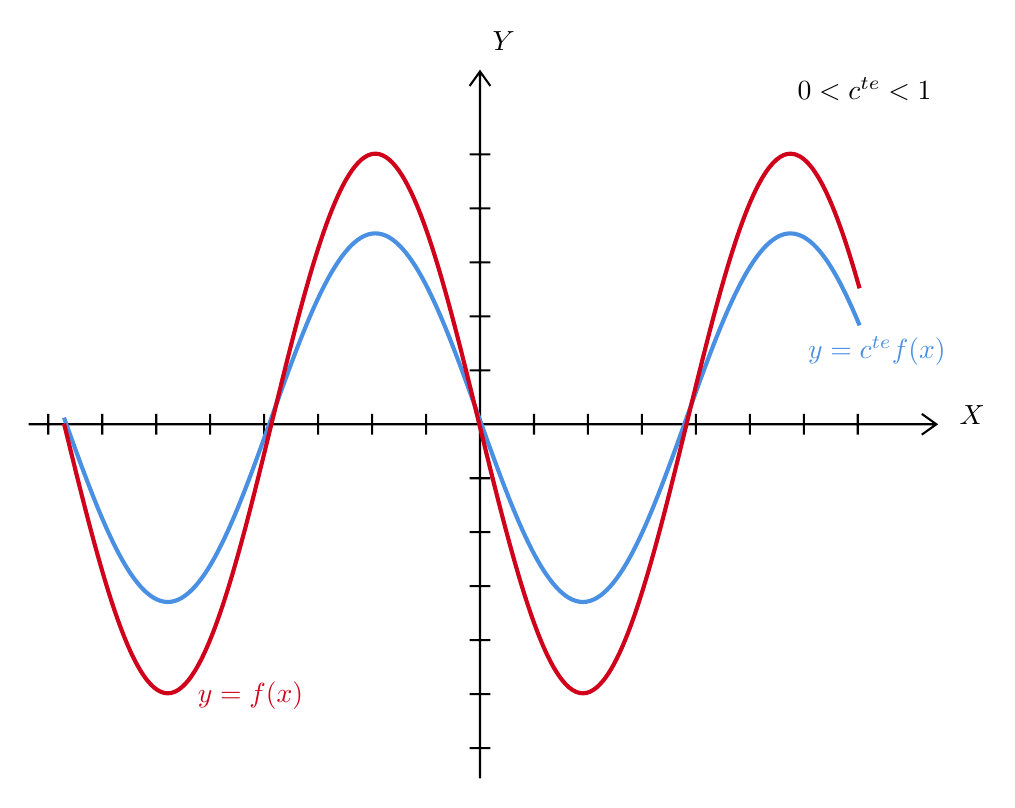
\begin{tikzpicture}[x=0.75pt,y=0.75pt,yscale=-1,xscale=1]
			%uncomment if require: \path (0,771); %set diagram left start at 0, and has height of 771
			
			%Shape: Axis 2D [id:dp7636403352579628] 
			\draw  (64,220.97) -- (501.3,220.97)(281.43,51) -- (281.43,391.6) (494.3,215.97) -- (501.3,220.97) -- (494.3,225.97) (276.43,58) -- (281.43,51) -- (286.43,58) (307.43,215.97) -- (307.43,225.97)(333.43,215.97) -- (333.43,225.97)(359.43,215.97) -- (359.43,225.97)(385.43,215.97) -- (385.43,225.97)(411.43,215.97) -- (411.43,225.97)(437.43,215.97) -- (437.43,225.97)(463.43,215.97) -- (463.43,225.97)(255.43,215.97) -- (255.43,225.97)(229.43,215.97) -- (229.43,225.97)(203.43,215.97) -- (203.43,225.97)(177.43,215.97) -- (177.43,225.97)(151.43,215.97) -- (151.43,225.97)(125.43,215.97) -- (125.43,225.97)(99.43,215.97) -- (99.43,225.97)(73.43,215.97) -- (73.43,225.97)(276.43,194.97) -- (286.43,194.97)(276.43,168.97) -- (286.43,168.97)(276.43,142.97) -- (286.43,142.97)(276.43,116.97) -- (286.43,116.97)(276.43,90.97) -- (286.43,90.97)(276.43,246.97) -- (286.43,246.97)(276.43,272.97) -- (286.43,272.97)(276.43,298.97) -- (286.43,298.97)(276.43,324.97) -- (286.43,324.97)(276.43,350.97) -- (286.43,350.97)(276.43,376.97) -- (286.43,376.97) ;
			\draw   ;
			%Shape: Wave [id:dp935589976697009] 
			\draw  [color={rgb, 255:red, 74; green, 144; blue, 226 }  ,draw opacity=1 ][line width=1.5]  (81,217.8) .. controls (97.31,263.29) and (112.9,306.6) .. (131,306.6) .. controls (149.1,306.6) and (164.69,263.29) .. (181,217.8) .. controls (197.31,172.31) and (212.9,129) .. (231,129) .. controls (249.1,129) and (264.69,172.31) .. (281,217.8) .. controls (297.31,263.29) and (312.9,306.6) .. (331,306.6) .. controls (349.1,306.6) and (364.69,263.29) .. (381,217.8) .. controls (397.31,172.31) and (412.9,129) .. (431,129) .. controls (442.87,129) and (453.67,147.65) .. (464.3,173.32) ;
			%Shape: Wave [id:dp7617198593557306] 
			\draw  [color={rgb, 255:red, 208; green, 2; blue, 27 }  ,draw opacity=1 ][line width=1.5]  (81,220.6) .. controls (97.31,287.2) and (112.9,350.6) .. (131,350.6) .. controls (149.1,350.6) and (164.69,287.2) .. (181,220.6) .. controls (197.31,154) and (212.9,90.6) .. (231,90.6) .. controls (249.1,90.6) and (264.69,154) .. (281,220.6) .. controls (297.31,287.2) and (312.9,350.6) .. (331,350.6) .. controls (349.1,350.6) and (364.69,287.2) .. (381,220.6) .. controls (397.31,154) and (412.9,90.6) .. (431,90.6) .. controls (442.87,90.6) and (453.67,117.9) .. (464.3,155.48) ;
			
			% Text Node
			\draw (286,30.4) node [anchor=north west][inner sep=0.75pt]    {$Y$};
			% Text Node
			\draw (511,210.4) node [anchor=north west][inner sep=0.75pt]    {$X$};
			% Text Node
			\draw (144,343.4) node [anchor=north west][inner sep=0.75pt]  [color={rgb, 255:red, 208; green, 2; blue, 27 }  ,opacity=1 ]  {$y=f( x)$};
			% Text Node
			\draw (438,177.4) node [anchor=north west][inner sep=0.75pt]  [color={rgb, 255:red, 74; green, 144; blue, 226 }  ,opacity=1 ]  {$y=c^{te} f( x)$};
			% Text Node
			\draw (433,52.4) node [anchor=north west][inner sep=0.75pt]  [color={rgb, 255:red, 0; green, 0; blue, 0 }  ,opacity=1 ]  {$0< c^{te} < 1$};
			
			\end{tikzpicture}
			\vspace*{3mm}
			\caption{Example of vertical compression of a function}
		\end{figure}
		To stretch or compress a function horizontally, by the same way, we just need to multiply the variable $x$ by a constant $c^{te}>1$ and respectively $0< c^{te}<1$ as:
		
		This is graphically represented for the case $0<c^{te}<1$ by:
		\begin{figure}[H]
			\centering
			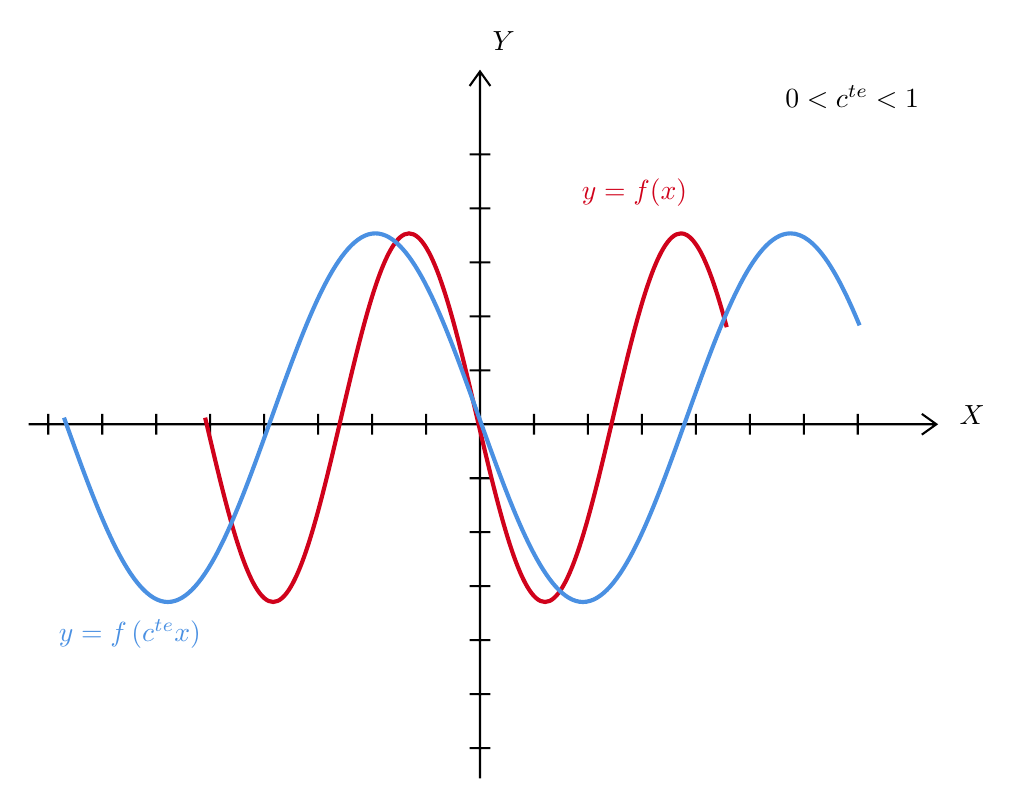
\begin{tikzpicture}[x=0.75pt,y=0.75pt,yscale=-1,xscale=1]
			%uncomment if require: \path (0,771); %set diagram left start at 0, and has height of 771
			
			%Shape: Axis 2D [id:dp7636403352579628] 
			\draw  (64,220.97) -- (501.3,220.97)(281.43,51) -- (281.43,391.6) (494.3,215.97) -- (501.3,220.97) -- (494.3,225.97) (276.43,58) -- (281.43,51) -- (286.43,58) (307.43,215.97) -- (307.43,225.97)(333.43,215.97) -- (333.43,225.97)(359.43,215.97) -- (359.43,225.97)(385.43,215.97) -- (385.43,225.97)(411.43,215.97) -- (411.43,225.97)(437.43,215.97) -- (437.43,225.97)(463.43,215.97) -- (463.43,225.97)(255.43,215.97) -- (255.43,225.97)(229.43,215.97) -- (229.43,225.97)(203.43,215.97) -- (203.43,225.97)(177.43,215.97) -- (177.43,225.97)(151.43,215.97) -- (151.43,225.97)(125.43,215.97) -- (125.43,225.97)(99.43,215.97) -- (99.43,225.97)(73.43,215.97) -- (73.43,225.97)(276.43,194.97) -- (286.43,194.97)(276.43,168.97) -- (286.43,168.97)(276.43,142.97) -- (286.43,142.97)(276.43,116.97) -- (286.43,116.97)(276.43,90.97) -- (286.43,90.97)(276.43,246.97) -- (286.43,246.97)(276.43,272.97) -- (286.43,272.97)(276.43,298.97) -- (286.43,298.97)(276.43,324.97) -- (286.43,324.97)(276.43,350.97) -- (286.43,350.97)(276.43,376.97) -- (286.43,376.97) ;
			\draw   ;
			%Shape: Wave [id:dp2679785641829078] 
			\draw  [color={rgb, 255:red, 208; green, 2; blue, 27 }  ,draw opacity=1 ][line width=1.5]  (149,217.8) .. controls (159.68,263.29) and (169.9,306.6) .. (181.75,306.6) .. controls (193.6,306.6) and (203.82,263.29) .. (214.5,217.8) .. controls (225.18,172.31) and (235.4,129) .. (247.25,129) .. controls (259.1,129) and (269.32,172.31) .. (280,217.8) .. controls (290.68,263.29) and (300.9,306.6) .. (312.75,306.6) .. controls (324.6,306.6) and (334.82,263.29) .. (345.5,217.8) .. controls (356.18,172.31) and (366.4,129) .. (378.25,129) .. controls (386.12,129) and (393.26,148.07) .. (400.3,174.2) ;
			%Shape: Wave [id:dp935589976697009] 
			\draw  [color={rgb, 255:red, 74; green, 144; blue, 226 }  ,draw opacity=1 ][line width=1.5]  (81,217.8) .. controls (97.31,263.29) and (112.9,306.6) .. (131,306.6) .. controls (149.1,306.6) and (164.69,263.29) .. (181,217.8) .. controls (197.31,172.31) and (212.9,129) .. (231,129) .. controls (249.1,129) and (264.69,172.31) .. (281,217.8) .. controls (297.31,263.29) and (312.9,306.6) .. (331,306.6) .. controls (349.1,306.6) and (364.69,263.29) .. (381,217.8) .. controls (397.31,172.31) and (412.9,129) .. (431,129) .. controls (442.87,129) and (453.67,147.65) .. (464.3,173.32) ;
			
			% Text Node
			\draw (286,30.4) node [anchor=north west][inner sep=0.75pt]    {$Y$};
			% Text Node
			\draw (511,210.4) node [anchor=north west][inner sep=0.75pt]    {$X$};
			% Text Node
			\draw (329,101.4) node [anchor=north west][inner sep=0.75pt]  [color={rgb, 255:red, 208; green, 2; blue, 27 }  ,opacity=1 ]  {$y=f( x)$};
			% Text Node
			\draw (77,313.4) node [anchor=north west][inner sep=0.75pt]  [color={rgb, 255:red, 74; green, 144; blue, 226 }  ,opacity=1 ]  {$y=f\left( c^{te} x\right)$};
			% Text Node
			\draw (427,56.4) node [anchor=north west][inner sep=0.75pt]  [color={rgb, 255:red, 0; green, 0; blue, 0 }  ,opacity=1 ]  {$0< c^{te} < 1$};
			\end{tikzpicture}
			\vspace*{3mm}
			\caption{Example of horizontal stretch of a function}
		\end{figure}
		and when $c^{te}>1$ by:
		\begin{figure}[H]
			\centering
			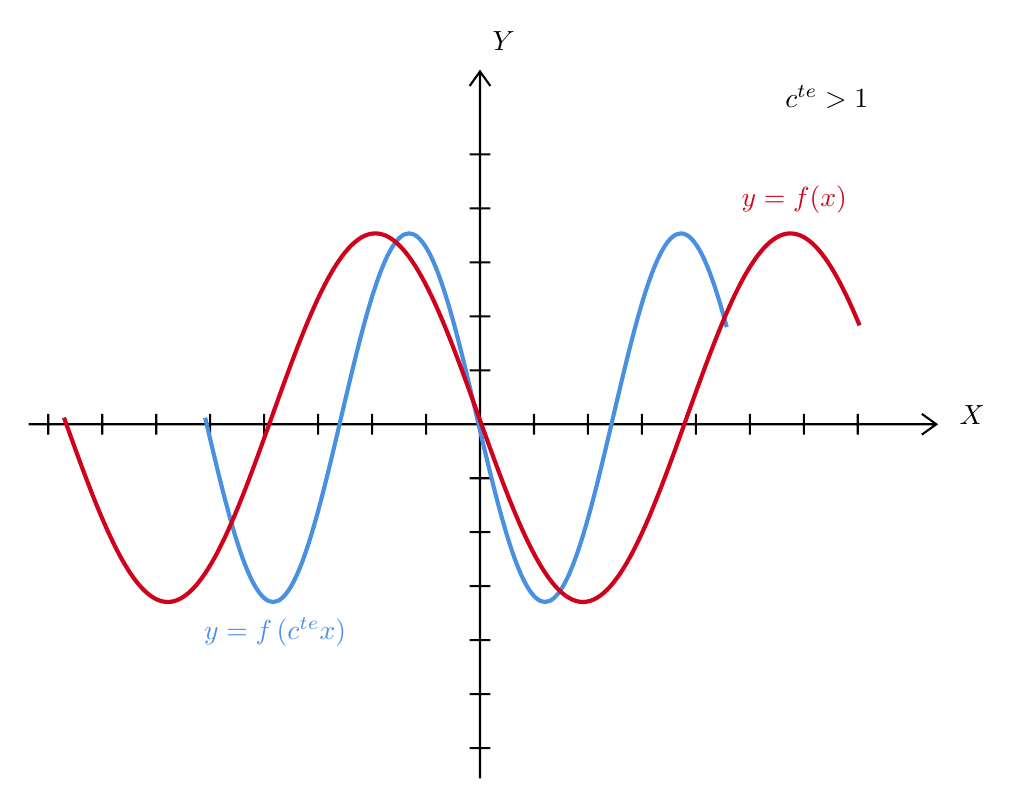
\begin{tikzpicture}[x=0.75pt,y=0.75pt,yscale=-1,xscale=1]
			%uncomment if require: \path (0,771); %set diagram left start at 0, and has height of 771
			
			%Shape: Axis 2D [id:dp7636403352579628] 
			\draw  (64,220.97) -- (501.3,220.97)(281.43,51) -- (281.43,391.6) (494.3,215.97) -- (501.3,220.97) -- (494.3,225.97) (276.43,58) -- (281.43,51) -- (286.43,58) (307.43,215.97) -- (307.43,225.97)(333.43,215.97) -- (333.43,225.97)(359.43,215.97) -- (359.43,225.97)(385.43,215.97) -- (385.43,225.97)(411.43,215.97) -- (411.43,225.97)(437.43,215.97) -- (437.43,225.97)(463.43,215.97) -- (463.43,225.97)(255.43,215.97) -- (255.43,225.97)(229.43,215.97) -- (229.43,225.97)(203.43,215.97) -- (203.43,225.97)(177.43,215.97) -- (177.43,225.97)(151.43,215.97) -- (151.43,225.97)(125.43,215.97) -- (125.43,225.97)(99.43,215.97) -- (99.43,225.97)(73.43,215.97) -- (73.43,225.97)(276.43,194.97) -- (286.43,194.97)(276.43,168.97) -- (286.43,168.97)(276.43,142.97) -- (286.43,142.97)(276.43,116.97) -- (286.43,116.97)(276.43,90.97) -- (286.43,90.97)(276.43,246.97) -- (286.43,246.97)(276.43,272.97) -- (286.43,272.97)(276.43,298.97) -- (286.43,298.97)(276.43,324.97) -- (286.43,324.97)(276.43,350.97) -- (286.43,350.97)(276.43,376.97) -- (286.43,376.97) ;
			\draw   ;
			%Shape: Wave [id:dp2679785641829078] 
			\draw  [color={rgb, 255:red, 74; green, 144; blue, 226 }  ,draw opacity=1 ][line width=1.5]  (149,217.8) .. controls (159.68,263.29) and (169.9,306.6) .. (181.75,306.6) .. controls (193.6,306.6) and (203.82,263.29) .. (214.5,217.8) .. controls (225.18,172.31) and (235.4,129) .. (247.25,129) .. controls (259.1,129) and (269.32,172.31) .. (280,217.8) .. controls (290.68,263.29) and (300.9,306.6) .. (312.75,306.6) .. controls (324.6,306.6) and (334.82,263.29) .. (345.5,217.8) .. controls (356.18,172.31) and (366.4,129) .. (378.25,129) .. controls (386.12,129) and (393.26,148.07) .. (400.3,174.2) ;
			%Shape: Wave [id:dp935589976697009] 
			\draw  [color={rgb, 255:red, 208; green, 2; blue, 27 }  ,draw opacity=1 ][line width=1.5]  (81,217.8) .. controls (97.31,263.29) and (112.9,306.6) .. (131,306.6) .. controls (149.1,306.6) and (164.69,263.29) .. (181,217.8) .. controls (197.31,172.31) and (212.9,129) .. (231,129) .. controls (249.1,129) and (264.69,172.31) .. (281,217.8) .. controls (297.31,263.29) and (312.9,306.6) .. (331,306.6) .. controls (349.1,306.6) and (364.69,263.29) .. (381,217.8) .. controls (397.31,172.31) and (412.9,129) .. (431,129) .. controls (442.87,129) and (453.67,147.65) .. (464.3,173.32) ;
			
			% Text Node
			\draw (286,30.4) node [anchor=north west][inner sep=0.75pt]    {$Y$};
			% Text Node
			\draw (511,210.4) node [anchor=north west][inner sep=0.75pt]    {$X$};
			% Text Node
			\draw (406,104.4) node [anchor=north west][inner sep=0.75pt]  [color={rgb, 255:red, 208; green, 2; blue, 27 }  ,opacity=1 ]  {$y=f( x)$};
			% Text Node
			\draw (147,312.4) node [anchor=north west][inner sep=0.75pt]  [color={rgb, 255:red, 74; green, 144; blue, 226 }  ,opacity=1 ]  {$y=f\left( c^{te} x\right)$};
			% Text Node
			\draw (427,56.4) node [anchor=north west][inner sep=0.75pt]  [color={rgb, 255:red, 0; green, 0; blue, 0 }  ,opacity=1 ]  {$c^{te}  >1$};
			\end{tikzpicture}
			\vspace*{3mm}
			\caption{Example of horizontal downscale of a function}
		\end{figure}
	\end{enumerate}
	
	\begin{tcolorbox}[title=Remark,arc=10pt,breakable,drop lifted shadow,
  skin=enhanced,
  skin first is subskin of={enhancedfirst}{arc=10pt,no shadow},
  skin middle is subskin of={enhancedmiddle}{arc=10pt,no shadow},
  skin last is subskin of={enhancedlast}{drop lifted shadow}]
	Translate, stretch, compress a function or apply it a symmetry is transforming it. The plot resulting from these transformations is named the "\NewTerm{transformed}\index{transformed graph}" from the initial plot.
	\end{tcolorbox}	
	
	\textbf{Definitions (\#\thesection.\mydef):} We say that a function $f$ is (we simplify the definition using an univariate function)\label{functions monotonicities}:
	\begin{itemize}
		\item[D1.] A "\NewTerm{constant function}\index{constant function}" on an interval $I$ if for each pair $(x_1,x_2)$ of elements of $I$ such that $x_1\neq x_2$, we have $f(x_1)=f(x_2)$. What we denote in a condensed manner by:
		
		
		\item[D2.] An "\NewTerm{increasing function}\index{increasing function}" or an "\NewTerm{increasing function in the broadest sense}" on the interval $I$ if for each pair $(x_1,x_2)$ of elements of $I$ such that $x_1\leq x_2$, we have $f(x_1)\leq f(x_2)$. What we denote in a condensed manner by:
		
		
		\item[D3.] A "\NewTerm{decreasing function}\index{decreasing function}" or an "\NewTerm{decreasing function in the broadest sense}" on the interval $I$ if for each pair $(x_1,x_2)$ of elements of $I$ such that $x_1\leq x_2$, we have $f(x_1)\geq f(x_2)$. What we denote in a condensed manner by:
		
		\begin{tcolorbox}[title=Remark,arc=10pt,breakable,drop lifted shadow,
  skin=enhanced,
  skin first is subskin of={enhancedfirst}{arc=10pt,no shadow},
  skin middle is subskin of={enhancedmiddle}{arc=10pt,no shadow},
  skin last is subskin of={enhancedlast}{drop lifted shadow}]
		A function is a "\NewTerm{monotonic function}\index{monotonic function}" or "\NewTerm{monotonic function in the broadest sense}" on an interval $I$ if it is increasing or decreasing in this interval.
		\end{tcolorbox}
		
		\item[D4.] A "\NewTerm{strictly increasing function}\index{strictly increasing function}" on the interval $I$ if for each pair $(x_1,x_2)$ of elements of $I$ such that $x_1\leq x_2$, we have $f(x_1)< f(x_2)$. What we denote in a condensed manner by:
		
		
		\item[D5.] A "\NewTerm{strictly decreasing function}\index{strictly decreasing function}" on the interval $I$ if for each pair $(x_1,x_2)$ of elements of $I$ such that $x_1\leq x_2$, we have $f(x_1)> f(x_2)$. What we denote in a condensed manner by:
		
		\begin{tcolorbox}[title=Remark,arc=10pt,breakable,drop lifted shadow,
  skin=enhanced,
  skin first is subskin of={enhancedfirst}{arc=10pt,no shadow},
  skin middle is subskin of={enhancedmiddle}{arc=10pt,no shadow},
  skin last is subskin of={enhancedlast}{drop lifted shadow}]
		A function is a "\NewTerm{strictly monotonic function}" on an interval $I$ if it is strictly increasing or decreasing in this interval.
		\end{tcolorbox}
	\end{itemize}
	Here's a visual summary of some of the monotonicity types defined above:
	\begin{figure}[H]
		\centering
		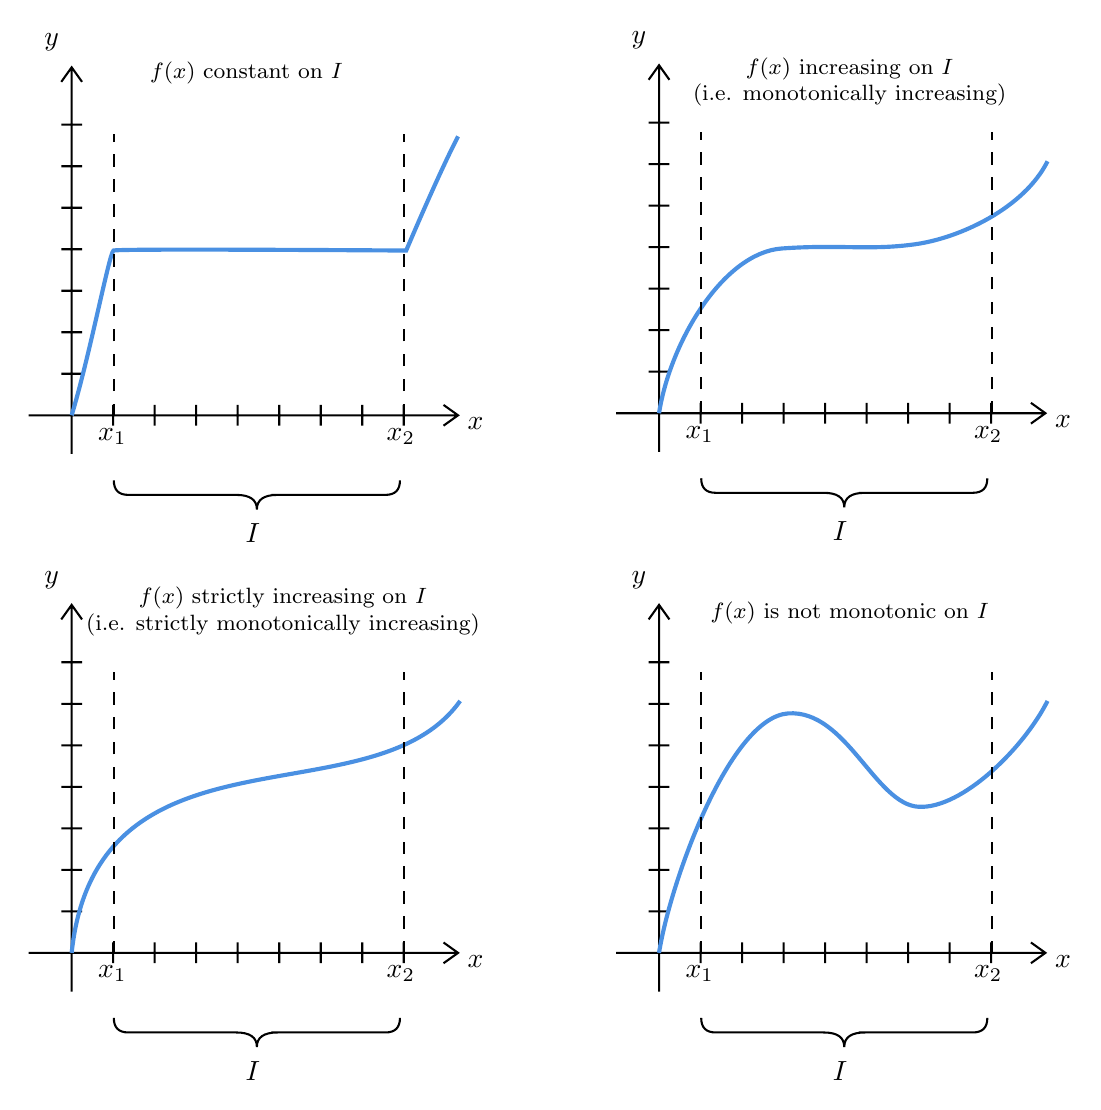
\begin{tikzpicture}[x=0.75pt,y=0.75pt,yscale=-1,xscale=1]
		%uncomment if require: \path (0,777); %set diagram left start at 0, and has height of 777
		
		%Shape: Axis 2D [id:dp7841069931442015] 
		\draw  (65,190.65) -- (271.86,190.65)(85.69,23) -- (85.69,209.28) (264.86,185.65) -- (271.86,190.65) -- (264.86,195.65) (80.69,30) -- (85.69,23) -- (90.69,30) (105.69,185.65) -- (105.69,195.65)(125.69,185.65) -- (125.69,195.65)(145.69,185.65) -- (145.69,195.65)(165.69,185.65) -- (165.69,195.65)(185.69,185.65) -- (185.69,195.65)(205.69,185.65) -- (205.69,195.65)(225.69,185.65) -- (225.69,195.65)(245.69,185.65) -- (245.69,195.65)(80.69,170.65) -- (90.69,170.65)(80.69,150.65) -- (90.69,150.65)(80.69,130.65) -- (90.69,130.65)(80.69,110.65) -- (90.69,110.65)(80.69,90.65) -- (90.69,90.65)(80.69,70.65) -- (90.69,70.65)(80.69,50.65) -- (90.69,50.65) ;
		\draw   ;
		%Shape: Brace [id:dp6935787250339556] 
		\draw   (106,222) .. controls (106,226.67) and (108.33,229) .. (113,229) -- (164.93,229) .. controls (171.6,229) and (174.93,231.33) .. (174.93,236) .. controls (174.93,231.33) and (178.26,229) .. (184.93,229)(181.93,229) -- (236.86,229) .. controls (241.53,229) and (243.86,226.67) .. (243.86,222) ;
		%Curve Lines [id:da8125706864760609] 
		\draw [color={rgb, 255:red, 74; green, 144; blue, 226 }  ,draw opacity=1 ][line width=1.5]    (85.69,190.65) .. controls (94.57,161.28) and (103.86,112.28) .. (105.86,111.28) .. controls (107.86,110.28) and (246.86,111.28) .. (246.86,111.28) .. controls (246.86,111.28) and (262.29,74.7) .. (271.86,56.28) ;
		%Straight Lines [id:da27499067876386696] 
		\draw  [dash pattern={on 4.5pt off 4.5pt}]  (106,191) -- (106,55.28) ;
		%Straight Lines [id:da37585209490162574] 
		\draw  [dash pattern={on 4.5pt off 4.5pt}]  (246,191) -- (246,55.28) ;
		%Shape: Axis 2D [id:dp3090811828252056] 
		\draw  (348,189.65) -- (554.86,189.65)(368.69,22) -- (368.69,208.28) (547.86,184.65) -- (554.86,189.65) -- (547.86,194.65) (363.69,29) -- (368.69,22) -- (373.69,29) (388.69,184.65) -- (388.69,194.65)(408.69,184.65) -- (408.69,194.65)(428.69,184.65) -- (428.69,194.65)(448.69,184.65) -- (448.69,194.65)(468.69,184.65) -- (468.69,194.65)(488.69,184.65) -- (488.69,194.65)(508.69,184.65) -- (508.69,194.65)(528.69,184.65) -- (528.69,194.65)(363.69,169.65) -- (373.69,169.65)(363.69,149.65) -- (373.69,149.65)(363.69,129.65) -- (373.69,129.65)(363.69,109.65) -- (373.69,109.65)(363.69,89.65) -- (373.69,89.65)(363.69,69.65) -- (373.69,69.65)(363.69,49.65) -- (373.69,49.65) ;
		\draw   ;
		%Shape: Brace [id:dp6118699399739407] 
		\draw   (389,221) .. controls (389,225.67) and (391.33,228) .. (396,228) -- (447.93,228) .. controls (454.6,228) and (457.93,230.33) .. (457.93,235) .. controls (457.93,230.33) and (461.26,228) .. (467.93,228)(464.93,228) -- (519.86,228) .. controls (524.53,228) and (526.86,225.67) .. (526.86,221) ;
		%Curve Lines [id:da529443541639059] 
		\draw [color={rgb, 255:red, 74; green, 144; blue, 226 }  ,draw opacity=1 ][line width=1.5]    (368.69,189.65) .. controls (374.17,154.84) and (399.86,112.28) .. (427.86,110.28) .. controls (455.86,108.28) and (469.86,111.28) .. (491.86,108.28) .. controls (513.86,105.28) and (544.67,90.66) .. (555.86,68.28) ;
		%Straight Lines [id:da9191294835873325] 
		\draw  [dash pattern={on 4.5pt off 4.5pt}]  (389,190) -- (389,54.28) ;
		%Straight Lines [id:da8561054132515158] 
		\draw  [dash pattern={on 4.5pt off 4.5pt}]  (529,190) -- (529,54.28) ;
		%Shape: Axis 2D [id:dp7904023891909902] 
		\draw  (65,449.65) -- (271.86,449.65)(85.69,282) -- (85.69,468.28) (264.86,444.65) -- (271.86,449.65) -- (264.86,454.65) (80.69,289) -- (85.69,282) -- (90.69,289) (105.69,444.65) -- (105.69,454.65)(125.69,444.65) -- (125.69,454.65)(145.69,444.65) -- (145.69,454.65)(165.69,444.65) -- (165.69,454.65)(185.69,444.65) -- (185.69,454.65)(205.69,444.65) -- (205.69,454.65)(225.69,444.65) -- (225.69,454.65)(245.69,444.65) -- (245.69,454.65)(80.69,429.65) -- (90.69,429.65)(80.69,409.65) -- (90.69,409.65)(80.69,389.65) -- (90.69,389.65)(80.69,369.65) -- (90.69,369.65)(80.69,349.65) -- (90.69,349.65)(80.69,329.65) -- (90.69,329.65)(80.69,309.65) -- (90.69,309.65) ;
		\draw   ;
		%Shape: Brace [id:dp9533276233669497] 
		\draw   (106,481) .. controls (106,485.67) and (108.33,488) .. (113,488) -- (164.93,488) .. controls (171.6,488) and (174.93,490.33) .. (174.93,495) .. controls (174.93,490.33) and (178.26,488) .. (184.93,488)(181.93,488) -- (236.86,488) .. controls (241.53,488) and (243.86,485.67) .. (243.86,481) ;
		%Curve Lines [id:da846465456727644] 
		\draw [color={rgb, 255:red, 74; green, 144; blue, 226 }  ,draw opacity=1 ][line width=1.5]    (85.69,449.65) .. controls (97.86,334.28) and (230.86,387.28) .. (272.86,328.28) ;
		%Straight Lines [id:da42370310462759386] 
		\draw  [dash pattern={on 4.5pt off 4.5pt}]  (106,450) -- (106,314.28) ;
		%Straight Lines [id:da47543511420460516] 
		\draw  [dash pattern={on 4.5pt off 4.5pt}]  (246,450) -- (246,314.28) ;
		%Shape: Axis 2D [id:dp13731858401802355] 
		\draw  (348,449.65) -- (554.86,449.65)(368.69,282) -- (368.69,468.28) (547.86,444.65) -- (554.86,449.65) -- (547.86,454.65) (363.69,289) -- (368.69,282) -- (373.69,289) (388.69,444.65) -- (388.69,454.65)(408.69,444.65) -- (408.69,454.65)(428.69,444.65) -- (428.69,454.65)(448.69,444.65) -- (448.69,454.65)(468.69,444.65) -- (468.69,454.65)(488.69,444.65) -- (488.69,454.65)(508.69,444.65) -- (508.69,454.65)(528.69,444.65) -- (528.69,454.65)(363.69,429.65) -- (373.69,429.65)(363.69,409.65) -- (373.69,409.65)(363.69,389.65) -- (373.69,389.65)(363.69,369.65) -- (373.69,369.65)(363.69,349.65) -- (373.69,349.65)(363.69,329.65) -- (373.69,329.65)(363.69,309.65) -- (373.69,309.65) ;
		\draw   ;
		%Shape: Brace [id:dp6765161909793536] 
		\draw   (389,481) .. controls (389,485.67) and (391.33,488) .. (396,488) -- (447.93,488) .. controls (454.6,488) and (457.93,490.33) .. (457.93,495) .. controls (457.93,490.33) and (461.26,488) .. (467.93,488)(464.93,488) -- (519.86,488) .. controls (524.53,488) and (526.86,485.67) .. (526.86,481) ;
		%Curve Lines [id:da7929816567775161] 
		\draw [color={rgb, 255:red, 74; green, 144; blue, 226 }  ,draw opacity=1 ][line width=1.5]    (368.69,449.65) .. controls (374.17,414.84) and (402.86,336.28) .. (430.86,334.28) .. controls (458.86,332.28) and (472.86,378.28) .. (493.86,379.28) .. controls (514.86,380.28) and (544.67,350.66) .. (555.86,328.28) ;
		%Straight Lines [id:da5130441064940936] 
		\draw  [dash pattern={on 4.5pt off 4.5pt}]  (389,450) -- (389,314.28) ;
		%Straight Lines [id:da06329814735074968] 
		\draw  [dash pattern={on 4.5pt off 4.5pt}]  (529,450) -- (529,314.28) ;
		
		% Text Node
		\draw (275,190.4) node [anchor=north west][inner sep=0.75pt]    {$x$};
		% Text Node
		\draw (71,5.4) node [anchor=north west][inner sep=0.75pt]    {$y$};
		% Text Node
		\draw (97,195.4) node [anchor=north west][inner sep=0.75pt]    {$x_{1}$};
		% Text Node
		\draw (236,195.4) node [anchor=north west][inner sep=0.75pt]    {$x_{2}$};
		% Text Node
		\draw (168,241.4) node [anchor=north west][inner sep=0.75pt]    {$I$};
		% Text Node
		\draw (122,19) node [anchor=north west][inner sep=0.75pt]  [font=\footnotesize] [align=left] {{\footnotesize $\displaystyle f(x)$ constant on $\displaystyle I$}};
		% Text Node
		\draw (558,189.4) node [anchor=north west][inner sep=0.75pt]    {$x$};
		% Text Node
		\draw (354,4.4) node [anchor=north west][inner sep=0.75pt]    {$y$};
		% Text Node
		\draw (380,194.4) node [anchor=north west][inner sep=0.75pt]    {$x_{1}$};
		% Text Node
		\draw (519,194.4) node [anchor=north west][inner sep=0.75pt]    {$x_{2}$};
		% Text Node
		\draw (451,240.4) node [anchor=north west][inner sep=0.75pt]    {$I$};
		% Text Node
		\draw (369,17) node [anchor=north west][inner sep=0.75pt]  [font=\footnotesize] [align=left] {\begin{minipage}[lt]{135pt}\setlength\topsep{0pt}
		\begin{center}
		{\footnotesize $\displaystyle f( x)$ increasing on $\displaystyle I$}\\{\footnotesize (i.e. monotonically increasing)}
		\end{center}
		
		\end{minipage}};
		% Text Node
		\draw (275,449.4) node [anchor=north west][inner sep=0.75pt]    {$x$};
		% Text Node
		\draw (71,264.4) node [anchor=north west][inner sep=0.75pt]    {$y$};
		% Text Node
		\draw (97,454.4) node [anchor=north west][inner sep=0.75pt]    {$x_{1}$};
		% Text Node
		\draw (236,454.4) node [anchor=north west][inner sep=0.75pt]    {$x_{2}$};
		% Text Node
		\draw (168,500.4) node [anchor=north west][inner sep=0.75pt]    {$I$};
		% Text Node
		\draw (76,272) node [anchor=north west][inner sep=0.75pt]  [font=\footnotesize] [align=left] {\begin{minipage}[lt]{165pt}\setlength\topsep{0pt}
		\begin{center}
		{\footnotesize $\displaystyle f( x)$ strictly increasing on $\displaystyle I$}\\{\footnotesize (i.e. strictly monotonically increasing)}
		\end{center}
		
		\end{minipage}};
		% Text Node
		\draw (558,449.4) node [anchor=north west][inner sep=0.75pt]    {$x$};
		% Text Node
		\draw (354,264.4) node [anchor=north west][inner sep=0.75pt]    {$y$};
		% Text Node
		\draw (380,454.4) node [anchor=north west][inner sep=0.75pt]    {$x_{1}$};
		% Text Node
		\draw (519,454.4) node [anchor=north west][inner sep=0.75pt]    {$x_{2}$};
		% Text Node
		\draw (451,500.4) node [anchor=north west][inner sep=0.75pt]    {$I$};
		% Text Node
		\draw (392,279) node [anchor=north west][inner sep=0.75pt]  [font=\footnotesize] [align=left] {{\footnotesize $\displaystyle f( x)$ is not monotonic on $\displaystyle I$}};
		\end{tikzpicture}
		\vspace*{3mm}
		\caption{Summary of some of the types of monocities of univariate functions}
	\end{figure}
	There are plenty of other existing visuals/charts representations. You can find in the thumbnail gallery below $206$ of them (excepted for two of them, they were all made with the \texttt{R} software and the code to create most of them is available in the corresponding companion book)\label{complete mosaic of charts type}:
	\begin{figure}[H]
		\centering
		\includegraphics[width=0.85\textwidth]{img/algebra/charts_gallery.jpg}
		\caption[Most common types of charts]{List of $206$ typical types of charts}
	\end{figure}
	However there is a few other existing charts used in practice and the reader interested in a more exhaustive list can take a look at the \textit{Type of Charts/Plots/Visuals} branch of the Data Science Mind Map at page \pageref{mindmap of data science}.
	
	\subsubsection{Analytical Representations}
	The analytical method of representation is by far the most used and consists of representing any function in an "\NewTerm{analytic expression}\index{analytic expression}" or "\NewTerm{closed form}\index{closed form}" which is a symbolic and abstract mathematical notation of all known mathematical operations that must be applied in a certain order to numbers and letters expressing constants or variables that we seek to analyse.
	
	Note that by "all known mathematical operations", we consider not only the mathematical operations seen in the chapter of Arithmetics (addition, subtraction, root extraction, etc.) but also all the operations that will be defined later in this book.
	
	If the functional dependence $y=f(x)$ is such that $f$ is an analytic expression, then we say that the "\NewTerm{function $y$ of $x$}" is "given analytically ". 

	Here are some examples of simple analytical expressions:
	
	When we have determined the equation of the mediator (see page \pageref{mediator analytic expression}), we have obtained an analytical expression of the visual straight line that characterize it as a function of the type:
	
	which we recall, is the analytical expression of the equation of a straight line, also named "\NewTerm{linear equation}\index{linear equation}" or "\NewTerm{affine function}\index{affine function}", on a plane where two points are known $P_1(x_1,y_1),P_2(x_2,y_2)$, the slope is given by the ratio of vertical growth on the horizontal growth as:
	
	A friendly and trivial application is to prove analytically that two non-vertical lines are parallel if and only if they have the same slope. Thus, given two lines with the equations:
	
	The lines intersect at a point $(x, y)$ if and only if values of $y$ are equal for a certain $x$, that is to say:
	
	The last equation can be solved with respect to $x$ if and only if $a_2-a_2\neq 0$. We have therefore proved that the lines $y_1,y_2$ intersect if and only if $a_1\neq a_2$. Therefore, they do not intersect (are parallel) if and only if $a_1=a_2$.
	
	In a quite simple way by applying the Pythagorean theorem, it is not difficult (\SeeChapter{see section Analytical Geometry page \pageref{conics}}) to determine that the equation of a circle with center $C (h, k)$ has for equation (it is of use in mathematics not explain $y$ for the equation of the circle therefore the equation of the latter is much more visually aesthetic and speaking):
	
	In these examples the functions are expressed analytically by a single formula (equality between two analytical expressions) which defines at the same time the "natural domain of definition" of the functions.
	
	\textbf{Definition (\#\thesection.\mydef):} The "\NewTerm{natural domain of definition}\index{natural domain of definition}\label{natural domain of definition}" of a function given by an analytical expression is the set of $x$ values for which the expression on the right-hand side has a definite value.
	
	For example the function:
	
	is defined for all values of $x$ except the value $x=1$ where we have a singularity (division by zero).
	\begin{tcolorbox}[title=Remark,arc=10pt,breakable,drop lifted shadow,
  skin=enhanced,
  skin first is subskin of={enhancedfirst}{arc=10pt,no shadow},
  skin middle is subskin of={enhancedmiddle}{arc=10pt,no shadow},
  skin last is subskin of={enhancedlast}{drop lifted shadow}]
	There are an infinite number of functions and we can not expose them all here, however we will meet more than a thousand on this entire book and should amply suffice to get an idea of their study.
	\end{tcolorbox}
	
	And we have the famous following "\NewTerm{table of variations}\index{table of variations}\label{table of variations}" that is also considered as an analytical tool and also used by some teachers to study the basics of the derivative $f'$ of a function $f$ (\SeeChapter{see section Differential and Integral Calculus page \pageref{differential calculus}}). For example with the function $x^3-3x^2+2$ (already seen in the previous mentioned section):

	\begin{minipage}{\linewidth}\centering
    \begin{variations}
     x      & \mI &    & 0 &    & 2 &    & \pI  \\
     \filet
     f'     & \ga +    & 0    &  -  &  0   & \dr+      \\
     \filet
     \m{f}  & ~  & \c  & \h{~} & \d & ~    &  \c       \\
     \end{variations}
	\end{minipage} 	
	
	Whose corresponding plot is:
	\begin{figure}[H]
		\centering
		\includegraphics{img/algebra/variation_plot_example.jpg}
		\caption[]{Plot of  function $x^3-3x^2+2$}
	\end{figure}
	
	\pagebreak
	\subsection{Functions}\label{functions}
	In mathematics, a function is a relation between a set of inputs and a set of permissible outputs with the property that each input is related to exactly one output.
	
	Functions of various kinds are the central objects of investigation in most fields of modern mathematics. There are many ways to describe or represent a function. Some functions may be defined by a formula or algorithm that tells how to compute the output for a given input. Others are given by a picture, named the "graph" of the function. In science, functions are sometimes defined by a table that gives the outputs for selected inputs. A function could be described implicitly, for example as the inverse to another function or as a solution of a differential equation.
	
	First remember the definitions already given earlier during our study of graphical representation of functions:
	
	\textbf{Definitions (\#\thesection.\mydef):} We say that a function $f$ is (we simplify the definition using an univariate function):
	\begin{itemize}
		\item[D1.] A function is a "\NewTerm{constant function}\index{constant function}" on an interval $I$ if for each pair $(x_1,x_2)$ of elements of $I$ such that $x_1\neq x_2$, we have $f(x_1)=f(x_2)$. What we denote in a condensed manner by:
		
		
		\item[D2.] A function is an "\NewTerm{increasing function}\index{increasing function}" or an "\NewTerm{increasing function in the broadest sense}" on the interval $I$ if for each pair $(x_1,x_2)$ of elements of $I$ such that $x_1\leq x_2$, we have $f(x_1)\leq f(x_2)$. What we denote in a condensed manner by:
		
		
		\item[D3.] A function is an "\NewTerm{decreasing function}\index{decreasing function}" or an "\NewTerm{decreasing function in the broadest sense}" on the interval $I$ if for each pair $(x_1,x_2)$ of elements of $I$ such that $x_1\leq x_2$, we have $f(x_1)\geq f(x_2)$. What we denote in a condensed manner by:
		
		\begin{tcolorbox}[title=Remark,arc=10pt,breakable,drop lifted shadow,
  skin=enhanced,
  skin first is subskin of={enhancedfirst}{arc=10pt,no shadow},
  skin middle is subskin of={enhancedmiddle}{arc=10pt,no shadow},
  skin last is subskin of={enhancedlast}{drop lifted shadow}]
		A function is a "\NewTerm{monotonic function}\index{monotonic function}" or "\NewTerm{monotonic function in the broadest sense}" on an interval $I$ if it is increasing or decreasing in this interval.
		\end{tcolorbox}
		
		\item[D4.] A function is a "\NewTerm{strictly increasing function}\index{strictly increasing function}" on the interval $I$ if for each pair $(x_1,x_2)$ of elements of $I$ such that $x_1\leq x_2$, we have $f(x_1)< f(x_2)$. What we denote in a condensed manner by:
		
		
		\item[D5.] A function is an "\NewTerm{strictly decreasing function}\index{strictly decreasing function}" on the interval $I$ if for each pair $(x_1,x_2)$ of elements of $I$ such that $x_1\leq x_2$, we have $f(x_1)> f(x_2)$. What we denote in a condensed manner by:
		
		\begin{tcolorbox}[title=Remark,arc=10pt,breakable,drop lifted shadow,
  skin=enhanced,
  skin first is subskin of={enhancedfirst}{arc=10pt,no shadow},
  skin middle is subskin of={enhancedmiddle}{arc=10pt,no shadow},
  skin last is subskin of={enhancedlast}{drop lifted shadow}]
		A function is a "\NewTerm{strictly monotonic function}\index{strictly monotonic function}" on an interval $I$ if it is strictly increasing or decreasing in this interval.
		\end{tcolorbox}
	\end{itemize}
	And let us add now complementary definitions:
	
	\textbf{Definitions (\#\thesection.\mydef):}
	\begin{enumerate}
		\item[D1.] We say that $y$ is a function of $x$ and we will write $y=f(x),y=\varphi(x)$, etc., if for every value of the variable $x$ belonging to a certain domain of definition (set) $D$, corresponds a value of the variable $y$ in another target domain of definition (set) $E$. What we denote in various ways (the third one being the most recommended):
		
		The variable $x$ is named "\NewTerm{independent variable}\index{independent variable}" or "\NewTerm{input variable}" or even "\NewTerm{exogenous variable}\index{exogenous variable}" and $y$ the "\NewTerm{dependent variable}\index{dependent variable}" or "\NewTerm{endogenous variable}\index{endogenous variable}".
		
		The dependence between the variables $x$ and $y$ is named a "\NewTerm{functional dependency}\index{functional dependency}". The letter $f$, which in the symbolic notation of functional dependence, indicates that we need to apply some operations to $x$ to obtain the corresponding $y$ value.
		
		Sometimes we write:
		
		rather than:
		
		In the latter case the letter $y$ expresses at the same time the value of the function and the symbol of operations applied to $x$.
		\begin{tcolorbox}[title=Remark,arc=10pt,breakable,drop lifted shadow,
  skin=enhanced,
  skin first is subskin of={enhancedfirst}{arc=10pt,no shadow},
  skin middle is subskin of={enhancedmiddle}{arc=10pt,no shadow},
  skin last is subskin of={enhancedlast}{drop lifted shadow}]
		As we saw it during our study in the section Set Theory, an application (or function) may be injective, surjective or bijective: 
		\begin{figure}[H]
			\centering
			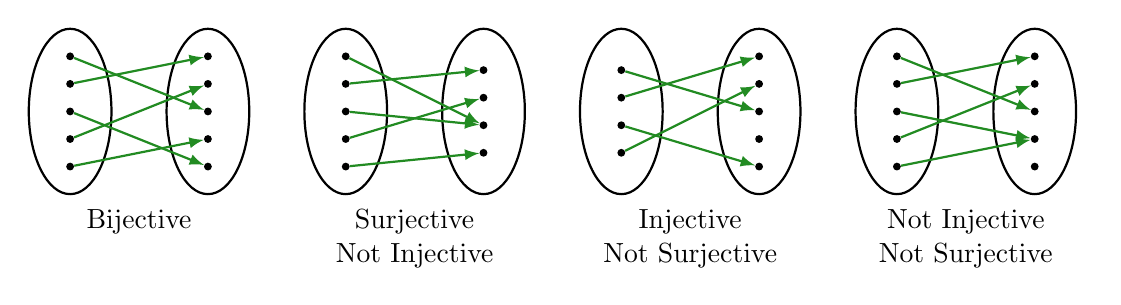
\begin{tikzpicture}[scale=0.35]
				\begin{scope}
				\draw[thick] (0,0) ellipse (1.5cm and 3cm);
				\draw[thick] (5,0) ellipse (1.5cm and 3cm);
				
				\node[fill,circle,scale=0.3] (a1) at (0,2) {};
				\node[fill,circle,scale=0.3] (a2) at (0,1) {};
				\node[fill,circle,scale=0.3] (a3) at (0,0) {};
				\node[fill,circle,scale=0.3] (a4) at (0,-1) {};
				\node[fill,circle,scale=0.3] (a5) at (0,-2) {};
				
				\node[fill,circle,scale=0.3] (b1) at (5,2) {};
				\node[fill,circle,scale=0.3] (b2) at (5,1) {};
				\node[fill,circle,scale=0.3] (b3) at (5,0) {};
				\node[fill,circle,scale=0.3] (b4) at (5,-1) {};
				\node[fill,circle,scale=0.3] (b5) at (5,-2) {};
				
				\draw[-latex,ForestGreen,thick] (a1)--(b3);
				\draw[-latex,ForestGreen,thick] (a2)--(b1);
				\draw[-latex,ForestGreen,thick] (a3)--(b5);
				\draw[-latex,ForestGreen,thick] (a4)--(b2);
				\draw[-latex,ForestGreen,thick] (a5)--(b4);
				
				\node[below] at (2.5,-3.2) {Bijective};
				\end{scope}
				
				\begin{scope}[xshift=10cm]
				\draw[thick] (0,0) ellipse (1.5cm and 3cm);
				\draw[thick] (5,0) ellipse (1.5cm and 3cm);
				
				\node[fill,circle,scale=0.3] (a1) at (0,2) {};
				\node[fill,circle,scale=0.3] (a2) at (0,1) {};
				\node[fill,circle,scale=0.3] (a3) at (0,0) {};
				\node[fill,circle,scale=0.3] (a4) at (0,-1) {};
				\node[fill,circle,scale=0.3] (a5) at (0,-2) {};
				
				\node[fill,circle,scale=0.3] (b1) at (5,1.5) {};
				\node[fill,circle,scale=0.3] (b2) at (5,.5) {};
				\node[fill,circle,scale=0.3] (b3) at (5,-0.5) {};
				\node[fill,circle,scale=0.3] (b4) at (5,-1.5) {}; 
				
				\draw[-latex,ForestGreen,thick] (a1)--(b3);
				\draw[-latex,ForestGreen,thick] (a2)--(b1);
				\draw[-latex,ForestGreen,thick] (a3)--(b3);
				\draw[-latex,ForestGreen,thick] (a4)--(b2);
				\draw[-latex,ForestGreen,thick] (a5)--(b4);
				
				\node[below, text width=3cm, align=center] at (2.5,-3.2) {Surjective \\ Not Injective};
				\end{scope}
				
				\begin{scope}[xshift=20cm]
				\draw[thick] (0,0) ellipse (1.5cm and 3cm);
				\draw[thick] (5,0) ellipse (1.5cm and 3cm);
				
				\node[fill,circle,scale=0.3] (a1) at (0,1.5) {};
				\node[fill,circle,scale=0.3] (a2) at (0,0.5) {};
				\node[fill,circle,scale=0.3] (a3) at (0,-0.5) {};
				\node[fill,circle,scale=0.3] (a4) at (0,-1.5) {}; 
				
				\node[fill,circle,scale=0.3] (b1) at (5,2) {};
				\node[fill,circle,scale=0.3] (b2) at (5,1) {};
				\node[fill,circle,scale=0.3] (b3) at (5,0) {};
				\node[fill,circle,scale=0.3] (b4) at (5,-1) {};
				\node[fill,circle,scale=0.3] (b5) at (5,-2) {};
				
				\draw[-latex,ForestGreen,thick] (a1)--(b3);
				\draw[-latex,ForestGreen,thick] (a2)--(b1);
				\draw[-latex,ForestGreen,thick] (a3)--(b5);
				\draw[-latex,ForestGreen,thick] (a4)--(b2); 
				
				\node[below, text width=3cm, align=center] at (2.5,-3.2) {Injective \\ Not Surjective};
				\end{scope}
				
				\begin{scope}[xshift=30cm]
				\draw[thick] (0,0) ellipse (1.5cm and 3cm);
				\draw[thick] (5,0) ellipse (1.5cm and 3cm);
				
				\node[fill,circle,scale=0.3] (a1) at (0,2) {};
				\node[fill,circle,scale=0.3] (a2) at (0,1) {};
				\node[fill,circle,scale=0.3] (a3) at (0,0) {};
				\node[fill,circle,scale=0.3] (a4) at (0,-1) {};
				\node[fill,circle,scale=0.3] (a5) at (0,-2) {};
				
				\node[fill,circle,scale=0.3] (b1) at (5,2) {};
				\node[fill,circle,scale=0.3] (b2) at (5,1) {};
				\node[fill,circle,scale=0.3] (b3) at (5,0) {};
				\node[fill,circle,scale=0.3] (b4) at (5,-1) {};
				\node[fill,circle,scale=0.3] (b5) at (5,-2) {};
				
				\draw[-latex,ForestGreen,thick] (a1)--(b3);
				\draw[-latex,ForestGreen,thick] (a2)--(b1);
				\draw[-latex,ForestGreen,thick] (a3)--(b4);
				\draw[-latex,ForestGreen,thick] (a4)--(b2);
				\draw[-latex,ForestGreen,thick] (a5)--(b4); 
				
				\node[below, text width=3cm, align=center] at (2.5,-3.2) {Not Injective \\ Not Surjective};
				\end{scope}
			\end{tikzpicture}
			\vspace*{3mm}
			\caption{Quick summary of applications/functions types}
		\end{figure}
		It is therefore necessary that the reader for whom these concepts are unknown goes in priority read these definitions.
		\end{tcolorbox}
		
		\item[D2.] The set of $x$ values (inputs) for which the value of the function $y$ is given by the function $f (x)$ is named the "\NewTerm{range of existence}\index{range of existence}" of the function or "\NewTerm{domain of definition}\index{domain of definition}\label{domain of definition}" of the function and denoted in this book by the letter $D$.
		
		The set of outputs of $f(x)$ is named the "\NewTerm{image}\index{image}" or sometimes the "\NewTerm{codomain}\index{codomain}" and denoted in this book by the letter $E$. When study of the point of view of the knowledge of the output values only, the set of $x$ is named the "\NewTerm{pre-image}".
		
		\item[D3.] A function $f(x)$ is named a "\NewTerm{periodic function}\index{periodic function}" if there is a constant $c^{te}$ such that the function's value does not change when we add (or subtract) that constant to the independent variable such as:
		
		which corresponds to a translation along the $x$-axis. The smallest constant satisfying this condition is named the "\NewTerm{period}\index{period}" of the function. It is frequently denoted by the letter $T$ in physics.
		
		The most common periodic functions know by students and engineers are the trigonometric functions (see section of the corresponding name page \pageref{trigonometry}):
		\begin{figure}[H]
			\centering
			\begin{tikzpicture}[x=0.75pt,y=0.75pt,yscale=-1,xscale=1]
			%uncomment if require: \path (0,670); %set diagram left start at 0, and has height of 670
			
			%Shape: Axis 2D [id:dp21573042822880728] 
			\draw  (190,291.6) -- (471.3,291.6)(216.39,38) -- (216.39,509.6) (464.3,286.6) -- (471.3,291.6) -- (464.3,296.6) (211.39,45) -- (216.39,38) -- (221.39,45) (266.39,286.6) -- (266.39,296.6)(316.39,286.6) -- (316.39,296.6)(366.39,286.6) -- (366.39,296.6)(416.39,286.6) -- (416.39,296.6)(211.39,241.6) -- (221.39,241.6)(211.39,191.6) -- (221.39,191.6)(211.39,141.6) -- (221.39,141.6)(211.39,91.6) -- (221.39,91.6)(211.39,341.6) -- (221.39,341.6)(211.39,391.6) -- (221.39,391.6)(211.39,441.6) -- (221.39,441.6)(211.39,491.6) -- (221.39,491.6) ;
			\draw   ;
			%Shape: Wave [id:dp332612481802524] 
			\draw  [color={rgb, 255:red, 74; green, 144; blue, 226 }  ,draw opacity=1 ][line width=1.5]  (206.3,352.7) .. controls (209.62,332.75) and (212.95,311.78) .. (216.3,290.6) .. controls (232.61,187.63) and (248.2,89.6) .. (266.3,89.6) .. controls (284.4,89.6) and (299.99,187.63) .. (316.3,290.6) .. controls (332.61,393.57) and (348.2,491.6) .. (366.3,491.6) .. controls (384.4,491.6) and (399.99,393.57) .. (416.3,290.6) .. controls (418.31,277.92) and (420.31,265.31) .. (422.3,252.95) ;
			%Straight Lines [id:da4020890705884055] 
			\draw [color={rgb, 255:red, 126; green, 211; blue, 33 }  ,draw opacity=1 ]   (266.3,94.6) -- (266.3,288.6) ;
			\draw [shift={(266.3,291.6)}, rotate = 270] [fill={rgb, 255:red, 126; green, 211; blue, 33 }  ,fill opacity=1 ][line width=0.08]  [draw opacity=0] (10.72,-5.15) -- (0,0) -- (10.72,5.15) -- (7.12,0) -- cycle    ;
			\draw [shift={(266.3,91.6)}, rotate = 90] [fill={rgb, 255:red, 126; green, 211; blue, 33 }  ,fill opacity=1 ][line width=0.08]  [draw opacity=0] (10.72,-5.15) -- (0,0) -- (10.72,5.15) -- (7.12,0) -- cycle    ;
			%Straight Lines [id:da02133492194790576] 
			\draw [color={rgb, 255:red, 189; green, 16; blue, 224 }  ,draw opacity=1 ]   (222.3,370.6) -- (412.3,370.6) ;
			\draw [shift={(415.3,370.6)}, rotate = 180] [fill={rgb, 255:red, 189; green, 16; blue, 224 }  ,fill opacity=1 ][line width=0.08]  [draw opacity=0] (10.72,-5.15) -- (0,0) -- (10.72,5.15) -- (7.12,0) -- cycle    ;
			\draw [shift={(219.3,370.6)}, rotate = 0] [fill={rgb, 255:red, 189; green, 16; blue, 224 }  ,fill opacity=1 ][line width=0.08]  [draw opacity=0] (10.72,-5.15) -- (0,0) -- (10.72,5.15) -- (7.12,0) -- cycle    ;
			
			% Text Node
			\draw (0,0) node [anchor=north west][inner sep=0.75pt]    {};
			\draw (476,290.4) node [anchor=north west][inner sep=0.75pt]    {$x$};
			% Text Node
			\draw (200,31.4) node [anchor=north west][inner sep=0.75pt]    {$y$};
			% Text Node
			\draw (200,184.4) node [anchor=north west][inner sep=0.75pt]    {$1$};
			% Text Node
			\draw (200,82.4) node [anchor=north west][inner sep=0.75pt]    {$2$};
			% Text Node
			\draw (257,298.4) node [anchor=north west][inner sep=0.75pt]    {$2\pi $};
			% Text Node
			\draw (310,298.4) node [anchor=north west][inner sep=0.75pt]    {$4\pi $};
			% Text Node
			\draw (358,298.4) node [anchor=north west][inner sep=0.75pt]    {$6\pi $};
			% Text Node
			\draw (408,298.4) node [anchor=north west][inner sep=0.75pt]    {$8\pi $};
			% Text Node
			\draw (1875	,383.4) node [anchor=north west][inner sep=0.75pt]    {$-1$};
			% Text Node
			\draw (187,483.4) node [anchor=north west][inner sep=0.75pt]    {$-2$};
			% Text Node
			\draw (268,177) node [anchor=north west][inner sep=0.75pt]  [color={rgb, 255:red, 126; green, 211; blue, 33 }  ,opacity=1 ] [align=left] {Amplitude $\displaystyle =2$};
			% Text Node
			\draw (423,218.4) node [anchor=north west][inner sep=0.75pt]  [color={rgb, 255:red, 74; green, 144; blue, 226 }  ,opacity=1 ]  {$y=2\sin\left(\frac{1}{4} x\right)$};
			% Text Node
			\draw (238,375) node [anchor=north west][inner sep=0.75pt]  [color={rgb, 255:red, 189; green, 16; blue, 224 }  ,opacity=1 ] [align=left] {Period$\displaystyle =8\pi $};
			\end{tikzpicture}
			\vspace*{3mm}
			\caption{Example of periodic function with period and amplitude}
		\end{figure}
		\begin{tcolorbox}[title=Remark,arc=10pt,breakable,drop lifted shadow,
  skin=enhanced,
  skin first is subskin of={enhancedfirst}{arc=10pt,no shadow},
  skin middle is subskin of={enhancedmiddle}{arc=10pt,no shadow},
  skin last is subskin of={enhancedlast}{drop lifted shadow}]
		The sum of two periodic functions with different periods is not necessarily periodic and there is no general formula to get the period of a function that is the sum of $n$ other functions!
		\end{tcolorbox}
		
		\item[D4.] In differential calculus (\SeeChapter{see section Differential and Integral Calculus page \pageref{differential calculus}}), the expression:
		
		with $h\neq 0$ is of particular interest. We name it a "\NewTerm{growth quotient}\index{growth quotient}" (we discuss this in much more detail in our study of differential and integral calculus).
		
		\item[D5.] We use certain properties of functions for easy graphical representation and analysis or mathematical simplifications. In particular, a function $f (x)$ is named "\NewTerm{even function}\index{even function}\label{even function}" if:
		
		for all $x$ in its definition domain.
		
		That is to say as we already seen previously, it is symmetric relatively with the $y$-axis:
		\begin{figure}[H]
			\centering
			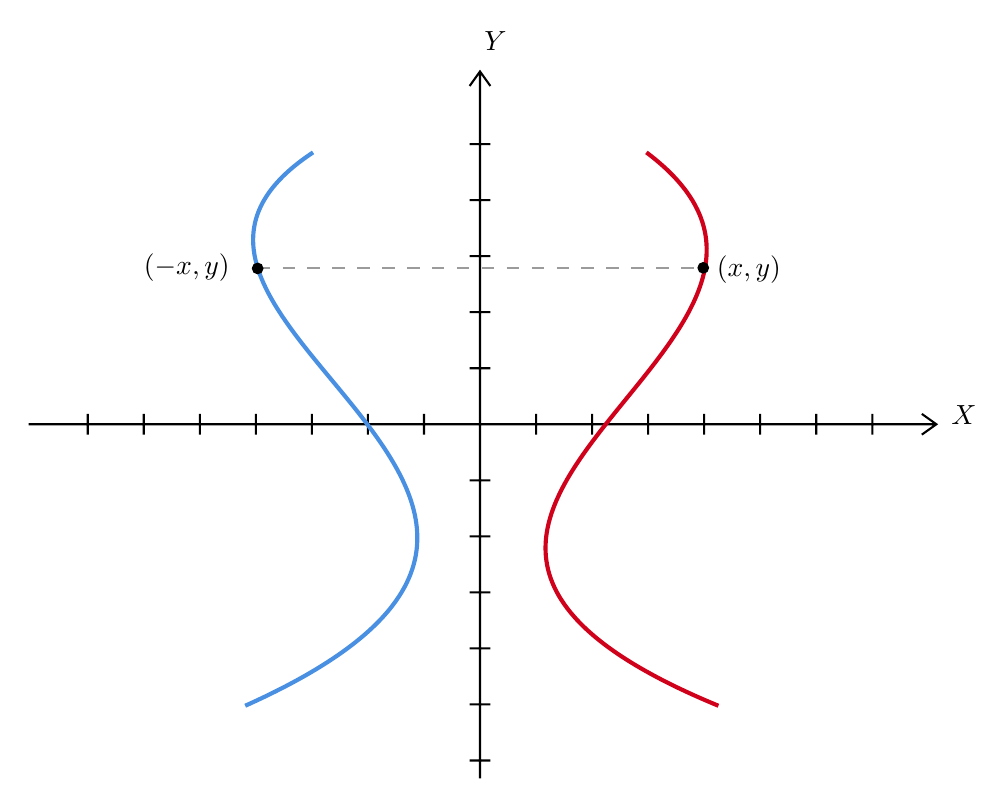
\begin{tikzpicture}[x=0.75pt,y=0.75pt,yscale=-1,xscale=1]
			%uncomment if require: \path (0,771); %set diagram left start at 0, and has height of 771
			
			%Shape: Axis 2D [id:dp7636403352579628] 
			\draw  (68,220.97) -- (505.3,220.97)(285.43,51) -- (285.43,391.6) (498.3,215.97) -- (505.3,220.97) -- (498.3,225.97) (280.43,58) -- (285.43,51) -- (290.43,58) (312.43,215.97) -- (312.43,225.97)(339.43,215.97) -- (339.43,225.97)(366.43,215.97) -- (366.43,225.97)(393.43,215.97) -- (393.43,225.97)(420.43,215.97) -- (420.43,225.97)(447.43,215.97) -- (447.43,225.97)(474.43,215.97) -- (474.43,225.97)(258.43,215.97) -- (258.43,225.97)(231.43,215.97) -- (231.43,225.97)(204.43,215.97) -- (204.43,225.97)(177.43,215.97) -- (177.43,225.97)(150.43,215.97) -- (150.43,225.97)(123.43,215.97) -- (123.43,225.97)(96.43,215.97) -- (96.43,225.97)(280.43,193.97) -- (290.43,193.97)(280.43,166.97) -- (290.43,166.97)(280.43,139.97) -- (290.43,139.97)(280.43,112.97) -- (290.43,112.97)(280.43,85.97) -- (290.43,85.97)(280.43,247.97) -- (290.43,247.97)(280.43,274.97) -- (290.43,274.97)(280.43,301.97) -- (290.43,301.97)(280.43,328.97) -- (290.43,328.97)(280.43,355.97) -- (290.43,355.97)(280.43,382.97) -- (290.43,382.97) ;
			\draw   ;
			%Curve Lines [id:da7098043564145642] 
			\draw [color={rgb, 255:red, 74; green, 144; blue, 226 }  ,draw opacity=1 ][line width=1.5]    (172.3,356.6) .. controls (395.3,256.6) and (84.3,169.6) .. (205,90) ;
			%Curve Lines [id:da31688466428341844] 
			\draw [color={rgb, 255:red, 208; green, 2; blue, 27 }  ,draw opacity=1 ][line width=1.5]    (400.3,356.6) .. controls (177.3,264.6) and (486.3,180.6) .. (365.6,90) ;
			%Straight Lines [id:da5040595412454372] 
			\draw [color={rgb, 255:red, 155; green, 155; blue, 155 }  ,draw opacity=1 ] [dash pattern={on 4.5pt off 4.5pt}]  (178.3,145.6) -- (395.3,145.6) ;
			%Shape: Circle [id:dp21608464408795736] 
			\draw  [fill={rgb, 255:red, 0; green, 0; blue, 0 }  ,fill opacity=1 ] (176,145.9) .. controls (176,144.63) and (177.03,143.6) .. (178.3,143.6) .. controls (179.57,143.6) and (180.6,144.63) .. (180.6,145.9) .. controls (180.6,147.17) and (179.57,148.2) .. (178.3,148.2) .. controls (177.03,148.2) and (176,147.17) .. (176,145.9) -- cycle ;
			%Shape: Circle [id:dp17037014344743073] 
			\draw  [fill={rgb, 255:red, 0; green, 0; blue, 0 }  ,fill opacity=1 ] (390.7,145.6) .. controls (390.7,144.33) and (391.73,143.3) .. (393,143.3) .. controls (394.27,143.3) and (395.3,144.33) .. (395.3,145.6) .. controls (395.3,146.87) and (394.27,147.9) .. (393,147.9) .. controls (391.73,147.9) and (390.7,146.87) .. (390.7,145.6) -- cycle ;
			
			% Text Node
			\draw (286,30.4) node [anchor=north west][inner sep=0.75pt]    {$Y$};
			% Text Node
			\draw (511,210.4) node [anchor=north west][inner sep=0.75pt]    {$X$};
			% Text Node
			\draw (122,137.4) node [anchor=north west][inner sep=0.75pt]    {$( -x,y)$};
			% Text Node
			\draw (398,138.4) node [anchor=north west][inner sep=0.75pt]    {$( x,y)$};
			\end{tikzpicture}
			\vspace*{3mm}
			\caption{Example of an even function}
		\end{figure}
		A function $f (x)$ is named "\NewTerm{odd function}\index{odd function}\label{odd function}" if:
		
		for all $x$ in its definition domain.
		
		That is to say as we already seen previously, it is symmetric relatively with the origin:
		\begin{figure}[H]
			\centering
			\begin{tikzpicture}[x=0.75pt,y=0.75pt,yscale=-1,xscale=1]
			%uncomment if require: \path (0,771); %set diagram left start at 0, and has height of 771
			
			%Shape: Axis 2D [id:dp7636403352579628] 
			\draw  (64,220.97) -- (501.3,220.97)(281.43,51) -- (281.43,391.6) (494.3,215.97) -- (501.3,220.97) -- (494.3,225.97) (276.43,58) -- (281.43,51) -- (286.43,58) (307.43,215.97) -- (307.43,225.97)(333.43,215.97) -- (333.43,225.97)(359.43,215.97) -- (359.43,225.97)(385.43,215.97) -- (385.43,225.97)(411.43,215.97) -- (411.43,225.97)(437.43,215.97) -- (437.43,225.97)(463.43,215.97) -- (463.43,225.97)(255.43,215.97) -- (255.43,225.97)(229.43,215.97) -- (229.43,225.97)(203.43,215.97) -- (203.43,225.97)(177.43,215.97) -- (177.43,225.97)(151.43,215.97) -- (151.43,225.97)(125.43,215.97) -- (125.43,225.97)(99.43,215.97) -- (99.43,225.97)(73.43,215.97) -- (73.43,225.97)(276.43,194.97) -- (286.43,194.97)(276.43,168.97) -- (286.43,168.97)(276.43,142.97) -- (286.43,142.97)(276.43,116.97) -- (286.43,116.97)(276.43,90.97) -- (286.43,90.97)(276.43,246.97) -- (286.43,246.97)(276.43,272.97) -- (286.43,272.97)(276.43,298.97) -- (286.43,298.97)(276.43,324.97) -- (286.43,324.97)(276.43,350.97) -- (286.43,350.97)(276.43,376.97) -- (286.43,376.97) ;
			\draw   ;
			%Curve Lines [id:da7098043564145642] 
			\draw [color={rgb, 255:red, 74; green, 144; blue, 226 }  ,draw opacity=1 ][line width=1.5]    (180.3,350.6) .. controls (403.3,250.6) and (4.6,319.2) .. (125.3,239.6) ;
			%Curve Lines [id:da31688466428341844] 
			\draw [color={rgb, 255:red, 208; green, 2; blue, 27 }  ,draw opacity=1 ][line width=1.5]    (437.3,200.6) .. controls (547.3,123.6) and (162.3,188.6) .. (381.3,90.6) ;
			%Straight Lines [id:da5040595412454372] 
			\draw [color={rgb, 255:red, 155; green, 155; blue, 155 }  ,draw opacity=1 ] [dash pattern={on 4.5pt off 4.5pt}]  (249.3,302.6) -- (312.3,136.6) ;
			%Shape: Circle [id:dp21608464408795736] 
			\draw  [fill={rgb, 255:red, 0; green, 0; blue, 0 }  ,fill opacity=1 ] (247.3,302.6) .. controls (247.3,301.33) and (248.33,300.3) .. (249.6,300.3) .. controls (250.87,300.3) and (251.9,301.33) .. (251.9,302.6) .. controls (251.9,303.87) and (250.87,304.9) .. (249.6,304.9) .. controls (248.33,304.9) and (247.3,303.87) .. (247.3,302.6) -- cycle ;
			%Shape: Circle [id:dp17037014344743073] 
			\draw  [fill={rgb, 255:red, 0; green, 0; blue, 0 }  ,fill opacity=1 ] (310,136.6) .. controls (310,135.33) and (311.03,134.3) .. (312.3,134.3) .. controls (313.57,134.3) and (314.6,135.33) .. (314.6,136.6) .. controls (314.6,137.87) and (313.57,138.9) .. (312.3,138.9) .. controls (311.03,138.9) and (310,137.87) .. (310,136.6) -- cycle ;
			
			% Text Node
			\draw (286,30.4) node [anchor=north west][inner sep=0.75pt]    {$Y$};
			% Text Node
			\draw (511,210.4) node [anchor=north west][inner sep=0.75pt]    {$X$};
			% Text Node
			\draw (181,297.4) node [anchor=north west][inner sep=0.75pt]    {$( -x,-y)$};
			% Text Node
			\draw (321,123.4) node [anchor=north west][inner sep=0.75pt]    {$( x,y)$};
			\end{tikzpicture}
			\vspace*{3mm}
			\caption{Example of an odd function}
		\end{figure}
		So, to summarize, an even function is a function that is independent of the sign of the variable and an odd function change of sign when we change the sign of the variable (the spiral of Cornus in the section Civil Engineering is a good practical example of odd function). This concept will be very useful to us to simplify some very useful developments in physics (such as Fourier transforms of odd or even functions for example, or the calculation of certain integrals!).
		\begin{theorem}
		Let us now show that any function $f(x)$ is the sum of an even function $g(x)$ and an odd function $h(x)$.
		
		\begin{tcolorbox}[title=Remark,arc=10pt,breakable,drop lifted shadow,
  skin=enhanced,
  skin first is subskin of={enhancedfirst}{arc=10pt,no shadow},
  skin middle is subskin of={enhancedmiddle}{arc=10pt,no shadow},
  skin last is subskin of={enhancedlast}{drop lifted shadow}]
		Remember that this type of theorem linking a general concept to a particular case and its opposite is often found in mathematics. We will see such examples in tensor calculus with the symmetric and antisymmetric tensor (\SeeChapter{see section Tensor Calculus page \pageref{symmetric tensor} and page \pageref{antisymmetric tensor}}) or in quantum physics with the Hermitian or non-Hermitian operators (\SeeChapter{see section Wave Quantum Physics page \pageref{hermitian operator} and page \pageref{non-hermitian operator}}).
		\end{tcolorbox}	
		\end{theorem}
		\begin{dem}
		Let us write:
		
		Then:
		
		If we sum then we get:
		
		and by subtracting:
		
		So there is really and odd and even decomposition of any function!!!
		\begin{flushright}
			$\blacksquare$  Q.E.D.
		\end{flushright}
		\end{dem}
		Finally, it is important to note that:
		\begin{itemize}
			\item The product of two even functions is an even function
			\item The product of two odd functions is an even function
			\item The product of an even and odd function is an odd function
		\end{itemize}
		Let us see a short proof of the last property because we will need it in the chapter on Geometry.
		\begin{dem}
		Let $g(x)$ be an even function and $h(x)$ an odd function such as:
		
		Therefore:
		
		\begin{flushright}
			$\blacksquare$  Q.E.D.
		\end{flushright}
		\end{dem}
		\item[D6.] In general, if $f (x)$ and $g (x)$ are arbitrary functions, we use the terminology and notations given in the following table:
		\begin{table}[H]	
			\centering
			\begin{tabular}{|c|c|}
			  \hline
			  \rowcolor[gray]{0.75}\textbf{Terminology}&\textbf{Value of the function}\\
			  \hline
			  % after \\: \hline or \cline{col1-col2} \cline{col3-col4} ...
			  Sum $f+g$ & $(f+g)(x)=f(x)+g(x)$ \\\hline
			  Difference $f-g$ & $(f-g)(x)=f(x)-g(x)$ \\\hline
			  Product $f \cdot g$ & $(f \cdot g)(x)=f(x)g(x)$ \\\hline
			  Quotient $\displaystyle\frac{f}{g}$&$\left(\displaystyle\frac{f}{g}\right)(x)=\displaystyle\frac{f(x)}{g(x)}$ \\\hline
			\end{tabular}
			\caption{Terminology about functions}
		\end{table}
		The definition domains of $f+g,f-g,f\cdot g$ are the intersection $I$ of the definition domain of $f (x)$ and $g(x)$, that is to say, the numbers which are common to both domains of definition. The domain of definition of $f/g$ is meanwhile the subset $I$ of all $x$ such that  $g(x)\neq 0$.
		
		\item[D7.] Let $y$ be a function of $f$ of $u$ such that $y=f(u)$ and $u$ a function $g$ of $x$ such that $u=g(x)$, then $y$ depends on $x$ and we have what we name a "\NewTerm{composite function}\index{composite function}\label{composite function}" that we denote:
		
		The last equality should be read "\NewTerm{$f$ round $g$}" and not confuse with the "round" symbol with the notation of the dot product that we have seen during our study of the section Vector Calculus page \pageref{dot product}.
		
		The domain of definition of the composite function is either identical to the entire domain of definition of the function $u=g(x)$ or the part of the domain in which the values of $u$ are such that the corresponding values $f (u)$ belong to the domain of definition of this function.
		
		Obviously the principle of composite function can be applied not only once, but an arbitrary number of times such that $y=f(g(h(t)))$ and so on...
		
		In computing science a function may compose with itself a given number of times $n$, such that $f(f(f(f(f\ldots )))))=f^n$ that must not be confuse with the power notation $f^n(x)$.
		
		If $u$ does not depend on another variable (or it is not itself a composite function), then we say that $f(u)$ is an "\NewTerm{elementary function}\index{elementary function}".

		Obviously there are an infinite number of elementary functions but most can be classified into families whose expression is similar to one of the following (here they are only univariate functions):
		\begin{itemize}
			\item "\NewTerm{Linear functions}\index{linear function}":
			
			They are simply functions representing straight lines of slope $a$ passing through the origin of the axis.
			
			\item "\NewTerm{Affine functions}\index{affine function}":
			
			They are simply functions representing straight lines of slope $a$ passing through the origin of the axis or not (linear function with a translation).
			\begin{figure}[H]
				\centering
				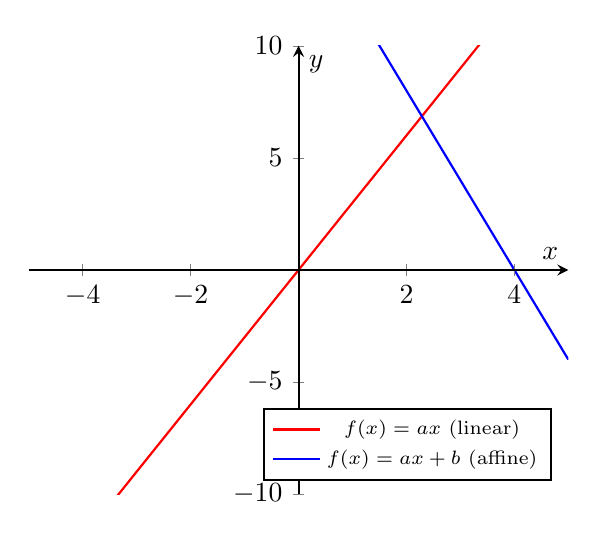
\begin{tikzpicture}
				\begin{axis}[
				%grid,
				%grid style={densely dashed},
				axis line style={->},
				axis lines=middle,
				xlabel=$x$,
				ylabel=$y$,
				xmin=-5, xmax=5,
				ymin=-10, ymax=10,
				axis lines=center,
				axis on top=true,
				domain=-5:5,
				legend style={font=\scriptsize},
				legend pos=south east
				]
				 \addplot [draw=red,thick] {3*x}; \addlegendentry{$f(x)=ax$ (linear)}
				 \addplot [draw=blue,thick] (x,-4*x+16); \addlegendentry{$f(x)=ax+b$ (affine)}
				\end{axis}
				\end{tikzpicture}
				\vspace*{3mm}
				\caption{Univariate affine and linear function}
			\end{figure}
						
			\item "\NewTerm{Power functions}\index{power function}":
			
			where $m\in\mathbb{R}$. Functions involving roots are often named "\NewTerm{radical functions}\index{radical functions}".
			\begin{figure}[H]
				\centering
				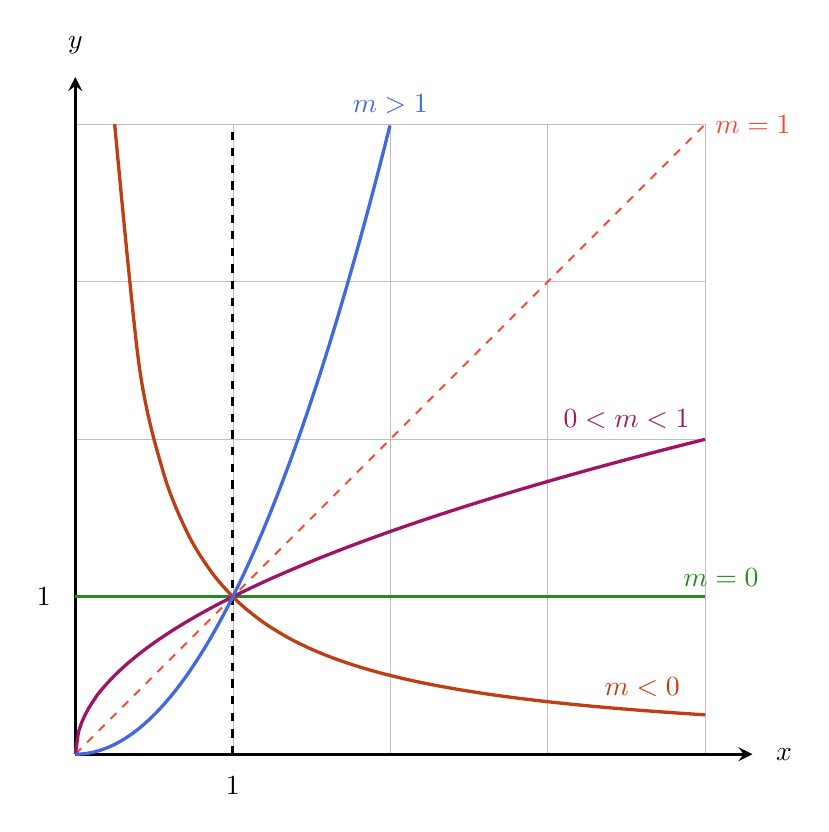
\begin{tikzpicture}[scale=2] 
				\draw[Gray!50, very thin] (0,0) grid (4,4);
				\draw[-stealth, very thick] (0,0)--(4.3,0);
				\draw[-stealth, very thick] (0,0)--(0,4.3);
				\node at (4.5,0) {$x$};
				\node at (0,4.5) {$y$};
				
				\node at (1,-0.2) {$1$};
				\node at (-0.2,1) {$1$};
				
				\node[right,RedOrange] at (4,4) {$m=1$};
				\draw[RedOrange,dashed] (0,0)--(4,4);
				\draw[Black,very thick,dashed] (1,0)--(1,4);
				
				\draw[domain=0:4,smooth,variable=\x, ForestGreen,very thick] plot ({\x},1);
				\node[above,ForestGreen] at (4.1,1) {$m=0$};
				\draw[domain=0.25:4,smooth,variable=\x, Bittersweet,very thick] plot ({\x},1/\x);
				\node[above,Bittersweet] at (3.6,0.3) {$m<0$};
				\draw[domain=0:4,samples=200,variable=\x, RedViolet,very thick] plot ({\x},\x^0.5);
				\node[above,RedViolet] at (3.5,2) {$0<m<1$};
				\draw[domain=0:2,samples=200,variable=\x, RoyalBlue,very thick] plot ({\x},\x^2);
				\node[above,RoyalBlue] at (2,4) {$m>1$};
				\end{tikzpicture}
				\vspace*{3mm}
				\caption{Different plots of simple power functions}
			\end{figure}
			
			\item "\NewTerm{Absolute value functions}\index{absolute value function}\label{absolute value plot}" (see section Arithmetic Operators page \pageref{absolute value} for the definition and the study of the "absolute value"):
			
			For example the plots with Maple 4.00b that we get with the command:\\
			
			\texttt{>plot([(x),(cos(x)),(x\string^2-3),(x\string^3-4*x\string^2+2*x)],x=-6..6,y=-4..3,\\
			thickness=3);}	
			
			\begin{figure}[H]
				\centering
				\includegraphics{img/analysis/pre_absolute_plot_functions.jpg}
			\end{figure}
			
			and taking the absolute value:\\
			
			\texttt{>plot([abs(x),abs(cos(x)),abs(x\string^2-3),abs(x\string^3-4*x\string^2+2*x)]\\
			,x=-6..6,y=-0.5..3,thickness=3);}
			\begin{figure}[H]
				\centering
				\includegraphics{img/analysis/post_absolute_plot_functions.jpg}
			\end{figure}
		
		\item "\NewTerm{Exponential functions}\index{exponential function}":
			
			where the famous $e^x$ is only a special case and also $a\in\mathbb{R}$.
			
			When $a\geq 0$ we have typically:
			\begin{figure}[H]
				\centering
				\includegraphics{img/analysis/exponential_functions.jpg}
				\caption{Different plots of simple exponential functions $(1^x,2^x,3^x,4^x)$ in Maple 4.00b}
			\end{figure}			
			If $a<0,x\in\mathbb{R}$ the function is not defined. Indeed for $(-1)^{0.5}=\left\lbrace \mathrm{i},	-\mathrm{i}	\right\rbrace$ therefore it is an application from $f:\mathbb{R}\mapsto\mathbb{C}^2$ and as far as we know there is no nice way to represent it visually and anyway this is not a function in the traditional way.
			
			\item "\NewTerm{Logarithmic functions}\index{logarithmic function}":
				
			with $a\in\mathbb{R}^{+}$ and that by construction of the logarithm (see further below) are of the type $f:\mathbb{R}^{+}\mapsto \mathbb{R}$.
			
			We have typically:
			\begin{figure}[H]
				\centering
				\includegraphics{img/analysis/logarithm_functions.jpg}
				\caption{Different plots of logarithm $\ln(x)=\ln_e(x)$ in green and $\log_{10}(x)$ in red with Maple 4.00b}
			\end{figure}
			
			\item "\NewTerm{Periodic/Trigonometric functions}\index{periodic function}\index{trigonometric function}":
			
			We already defined previously what is a periodic function. For the trigonometric functions the reader can see below a plot of the main one but for more details it is strongly recommended to read the section Trigonometry page \pageref{trigonometry}:
			\begin{figure}[H]
				\centering
				\includegraphics[scale=0.9]{img/analysis/trigonometric_functions.jpg}
				\caption{Different plots of trigonometric functions in Maple 4.00b}
			\end{figure}
			
			\item "\NewTerm{Polynomial functions}\index{polynomial function}":
			
			where as we already know $a_0,a_1,\ldots ,a_n$ are constant numbers named "\NewTerm{coefficients}\index{coefficients}" and $n$ is a positive integer that we name "\NewTerm{degree of the polynomial}\index{degree of a polynomial}" (\SeeChapter{voir section Calculus page \pageref{polynomial}}). Obviously this function is defined for all values of $x$, that is to say, it is define on an infinite interval.
			
			If follows that power functions of the type $x^m$ and linear functions of the type $f(x)=x$ are a subclass of polynomial for $m\in \mathbb{N}$.
			
			We have already studied more deeply polynomials in the section Calculus with their main properties but let us give again the plot of some of them as recall: 
			\begin{figure}[H]
				\centering
				\begin{subfigure}{.5\textwidth}
					\centering
				    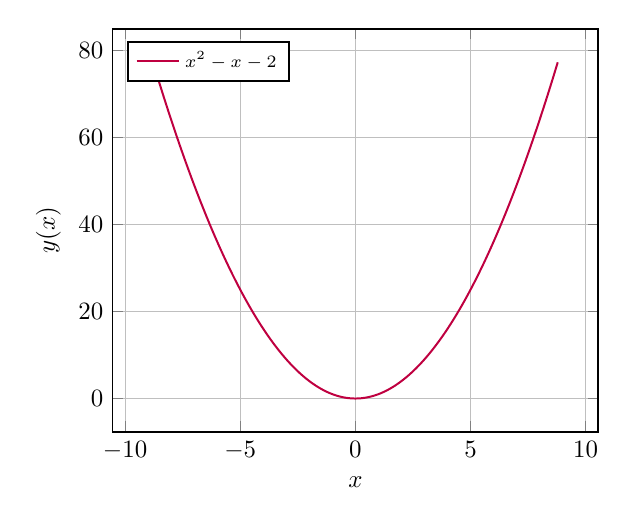
\begin{tikzpicture}[scale=0.9]
					\begin{axis}[domain=-10:10,
				    restrict y to domain=0:80,
				    samples=100,
				    grid=major,smooth,
				    xlabel=$x$,
				    ylabel=$y(x)$, 
				    legend pos=north west,
				    legend style={font=\scriptsize\selectfont}]
				
					\addplot [color=purple,thick] {x^2}; 
					\legend{${\footnotesize x^2-x-2}$}
					\end{axis}
					\end{tikzpicture}
				\end{subfigure}%
				\begin{subfigure}{.5\textwidth}
				    \centering
				    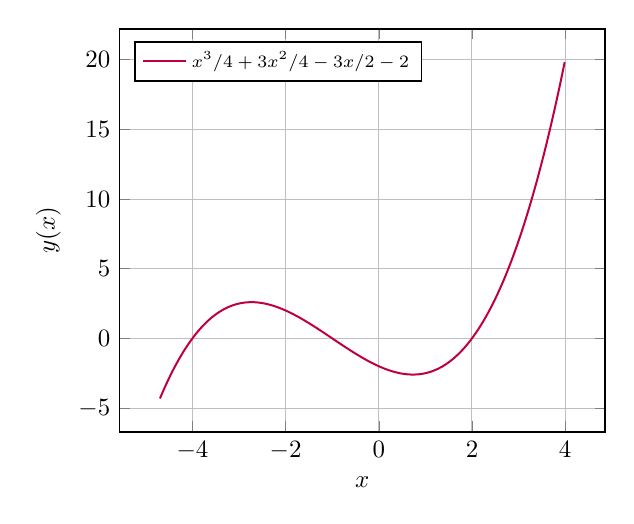
\begin{tikzpicture}[scale=0.9]
					\begin{axis}[domain=-5:5,
				    restrict y to domain=-5:20,
				    samples=100,
				    grid=major,smooth,
				    xlabel=$x$,
				    ylabel=$y(x)$, 
				    legend pos=north west,
				    legend style={font=\scriptsize\selectfont}]
				
					\addplot [color=purple,thick] {x^3/4+3*x^2/4-3*x/2-2}; 
					\legend{$x^3/4+3x^2/4-3x/2-2$}
					\end{axis}
					\end{tikzpicture}
				\end{subfigure}
			\end{figure}
			\begin{figure}[H]
				\centering
				\begin{subfigure}{.5\textwidth}
					\centering
				    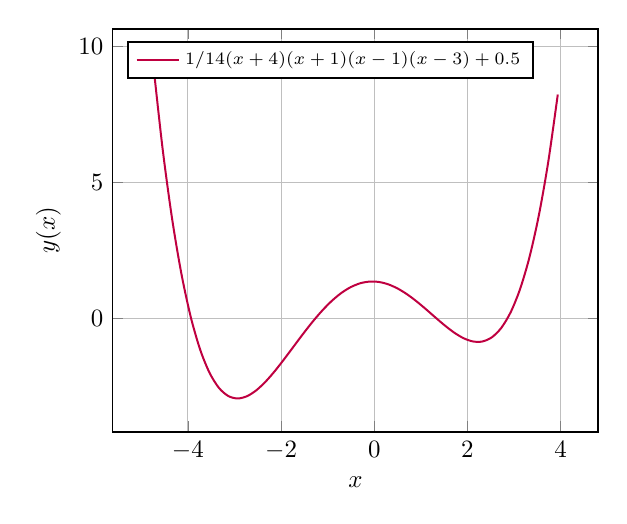
\begin{tikzpicture}[scale=0.9]
					\begin{axis}[domain=-10:10,
				    restrict y to domain=-10:10,
				    samples=100,
				    grid=major,smooth,
				    xlabel=$x$,
				    ylabel=$y(x)$, 
				    legend pos=north west,
				    legend style={font=\scriptsize\selectfont}]
				
					\addplot [color=purple,thick] {1/14*(x+4)*(x+1)*(x-1)*(x-3)+0.5}; 
					\legend{$1/14(x+4)(x+1)(x-1)(x-3)+0.5$}
					\end{axis}
					\end{tikzpicture}
				\end{subfigure}%
				\begin{subfigure}{.5\textwidth}
				    \centering
				    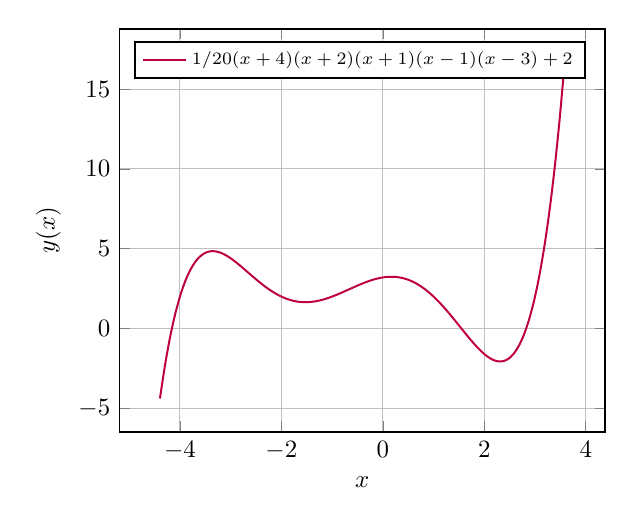
\begin{tikzpicture}[scale=0.9]
					\begin{axis}[domain=-5:5,
				    restrict y to domain=-5:20,
				    samples=100,
				    grid=major,smooth,
				    xlabel=$x$,
				    ylabel=$y(x)$, 
				    legend pos=north west,
				    legend style={font=\scriptsize\selectfont}]
				
					\addplot [color=purple,thick] {1/20*(x+4)*(x+2)*(x+1)*(x-1)*(x-3)+2}; 
					\legend{$1/20(x+4)(x+2)(x+1)(x-1)(x-3)+2$}
					\end{axis}
					\end{tikzpicture}
				\end{subfigure}
			\end{figure}
			\begin{figure}[H]
				\centering
				\begin{subfigure}{.5\textwidth}
					\centering
				    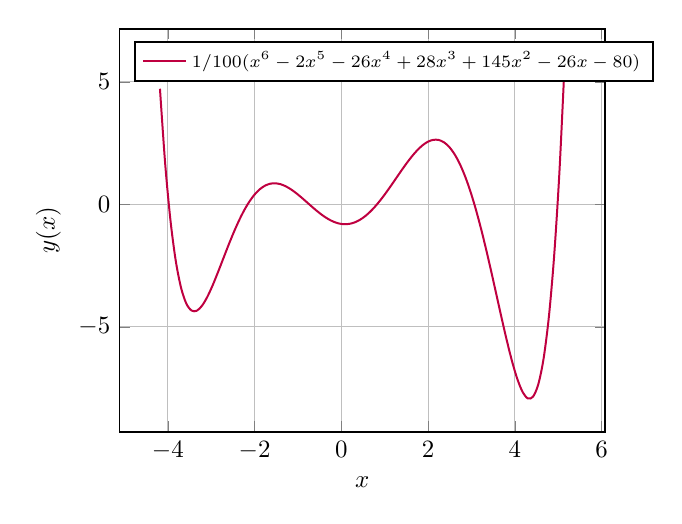
\begin{tikzpicture}[scale=0.9]
					\begin{axis}[domain=-6:6,
				    restrict y to domain=-8:8,
				    samples=100,
				    grid=major,smooth,
				    xlabel=$x$,
				    ylabel=$y(x)$, 
				    legend pos=north west,
				    legend style={font=\scriptsize\selectfont}]
				
					\addplot [color=purple,thick] {1/100*(x^6-2*x^5-26*x^4+28*x^3+145*x^2-26*x-80)}; 
					\legend{$1/100(x^6-2x^5-26x^4+28x^3+145x^2-26x-80)$}
					\end{axis}
					\end{tikzpicture}
				\end{subfigure}%
				\begin{subfigure}{.5\textwidth}
				    \centering
				    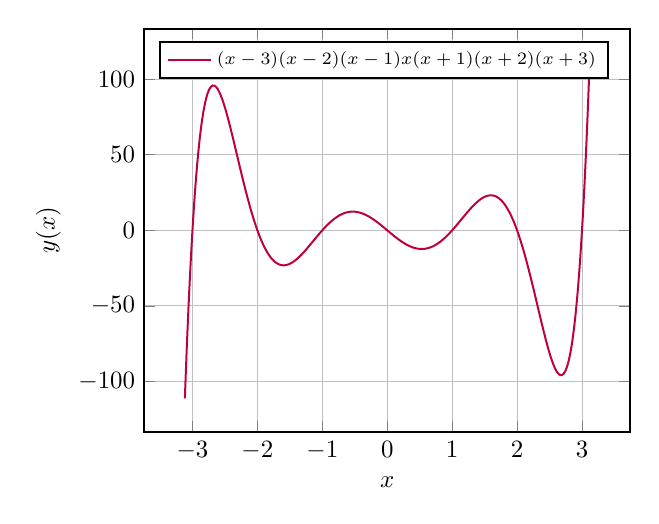
\begin{tikzpicture}[scale=0.9]
					\begin{axis}[domain=-4:4,
				    restrict y to domain=-120:120,
				    samples=300,
				    grid=major,smooth,
				    xlabel=$x$,
				    ylabel=$y(x)$, 
				    legend pos=north west,
				    legend style={font=\scriptsize\selectfont}]
				
					\addplot [color=purple,thick] {(x-3)*(x-2)*(x-1)*x*(x+1)*(x+2)*(x+3)}; 
					\legend{$(x-3)(x-2)(x-1)x(x+1)(x+2)(x+3)$}
					\end{axis}
					\end{tikzpicture}
				\end{subfigure}
				\caption{Some polynomials plotted with TikZ}
			\end{figure}
			We will see and study in this book some famous polynomials as the: Legendre polynomials (\SeeChapter{see section Quantum Chemistry page \pageref{legendre polynomial}}), Bernoulli polynomials (\SeeChapter{see section Sequences and Series page \pageref{bernoulli polynomials}}), Bernstein polynomials (\SeeChapter{see section Numerical Methods page \pageref{bernstein polynomial}}), Hermite polynomials (\SeeChapter{see section Functional Analysis page \pageref{hermite polynomial}}), ...
			
			\item "\NewTerm{Rational fractions}\index{rational fractions}" are polynomials divisions (\SeeChapter{see section Calculus page \pageref{polynomials division}}):
			
			\begin{tcolorbox}[title=Remark,arc=10pt,breakable,drop lifted shadow,
  skin=enhanced,
  skin first is subskin of={enhancedfirst}{arc=10pt,no shadow},
  skin middle is subskin of={enhancedmiddle}{arc=10pt,no shadow},
  skin last is subskin of={enhancedlast}{drop lifted shadow}]
			Obviously two rational fractions are equal, if one is obtained from the other by multiplying the numerator and denominator by the same polynomial.
			\end{tcolorbox}
			The rational function:
			
			is not defined at $x^2=5 \Leftrightarrow x=\pm \sqrt{5}$. It is asymptotic (see further below) to $\frac{x}{2}$ as $x$ approaches infinity:
			\begin{figure}[H]
				\centering
				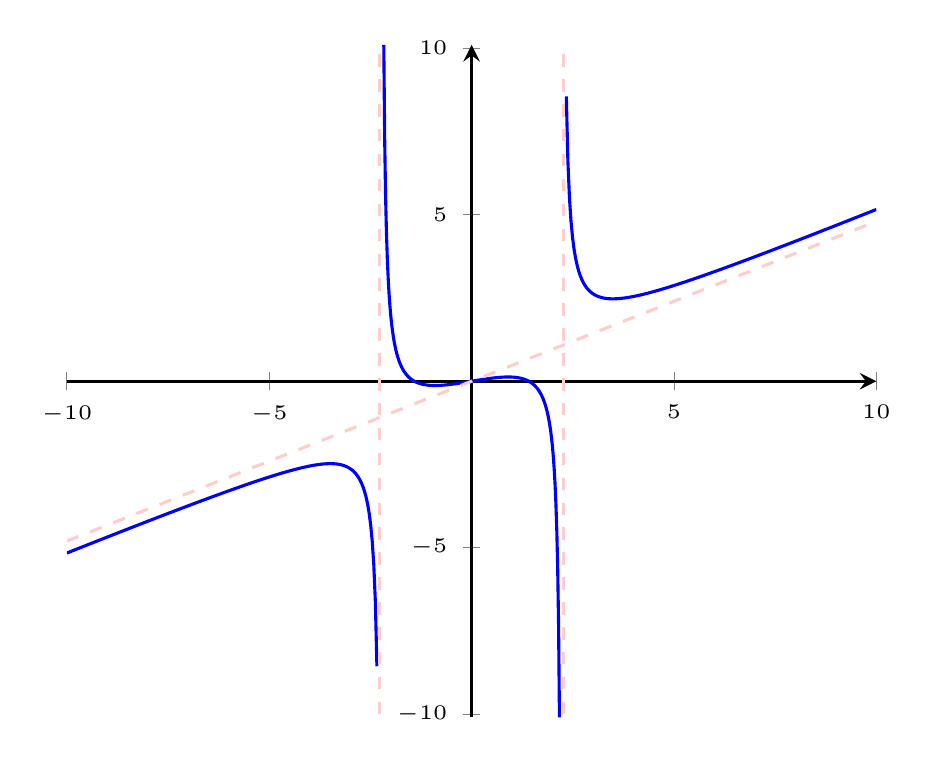
\begin{tikzpicture}[scale=1.5]
				\begin{axis}[
				  axis lines=middle,
				  samples=200,
				  tick label style={font=\tiny},
				  xtick={-10,-5,...,10},
				  ytick={-10,-5,...,10}
				]
				\addplot[blue,domain=-10:-2.34] {(x^3-2*x)/(2*(x^2-5))};
				\addplot[blue,domain=-2.17:2.17] {(x^3-2*x)/(2*(x^2-5))};
				\addplot[blue,domain=2.34:10] {(x^3-2*x)/(2*(x^2-5))};
				\draw[red!20,dashed] (axis cs:-10,-4.8) -- (axis cs:10,4.8);
				\draw[red!20,dashed] (axis cs:-2.28,-10) -- (axis cs:-2.28,10);
				\draw[red!20,dashed] (axis cs:2.28,-10) -- (axis cs:2.28,10);
				\end{axis}
				\end{tikzpicture}
				\vspace*{3mm}
				\caption[Example of a rational function]{Example of a rational function $f(x) = \frac{x^3-2x}{2(x^2-5)}$}
			\end{figure}
			The rational function:
			
			 is defined for all real numbers, but not for all complex numbers, since if x were a square root of $-1$ (i.e. the imaginary unit or its negative), then formal evaluation would lead to division by zero!
			 
			 \begin{tcolorbox}[title=Remarks,arc=10pt,breakable,drop lifted shadow,
  skin=enhanced,
		  skin first is subskin of={enhancedfirst}{arc=10pt,no shadow},
		  skin middle is subskin of={enhancedmiddle}{arc=10pt,no shadow},
		  skin last is subskin of={enhancedlast}{drop lifted shadow}]
			 A constant function is a rational function since constants are polynomials! Every polynomial function $f(x) = P(x)$ is a rational function with $Q(x) = 1$. The power functions $f(x)=x^m$ are also rational functions when $m\in\mathbb{N}$.
			\end{tcolorbox}
			 
			 \item "\NewTerm{Algebraic functions}\index{algebraic function}" are defined by the fact that the function $f(x)$ is the result of addition, subtraction, multiplication, division, of variables put to an integer or non-integer power. Therefore most of the functions defined previously can be included in this definition: linear functions, affine functions, power functions, polynomial functions, rational functions.
			 
			 \item "\NewTerm{Piecewise functions}\index{piecewise function}" is a function defined by different formulas on different parts of its domain. The absolute value is a famous example of a piecewise-defined function because the formula changes with the sign of $x$:
			 
			Another well-known example is the function that calculates pension contributions based on age. All countries (or companies) that have a pension concept have contribution amounts based on a piecewise continuous function.
			 
			 \item "\NewTerm{Step functions}\index{step function}" $f:[a,b]\in \mathbb{R}$ is defined if and only if there exists a subdivision $(a_i)_{0\leq i \leq n}$ of $[a, b]$ such that $a_0=a$ and $a_n=b$ and $(\lambda_0,\ldots ,\lambda_n)\in \mathbb{R}^n$ such as:
			 
			\begin{figure}[H]
				\centering
				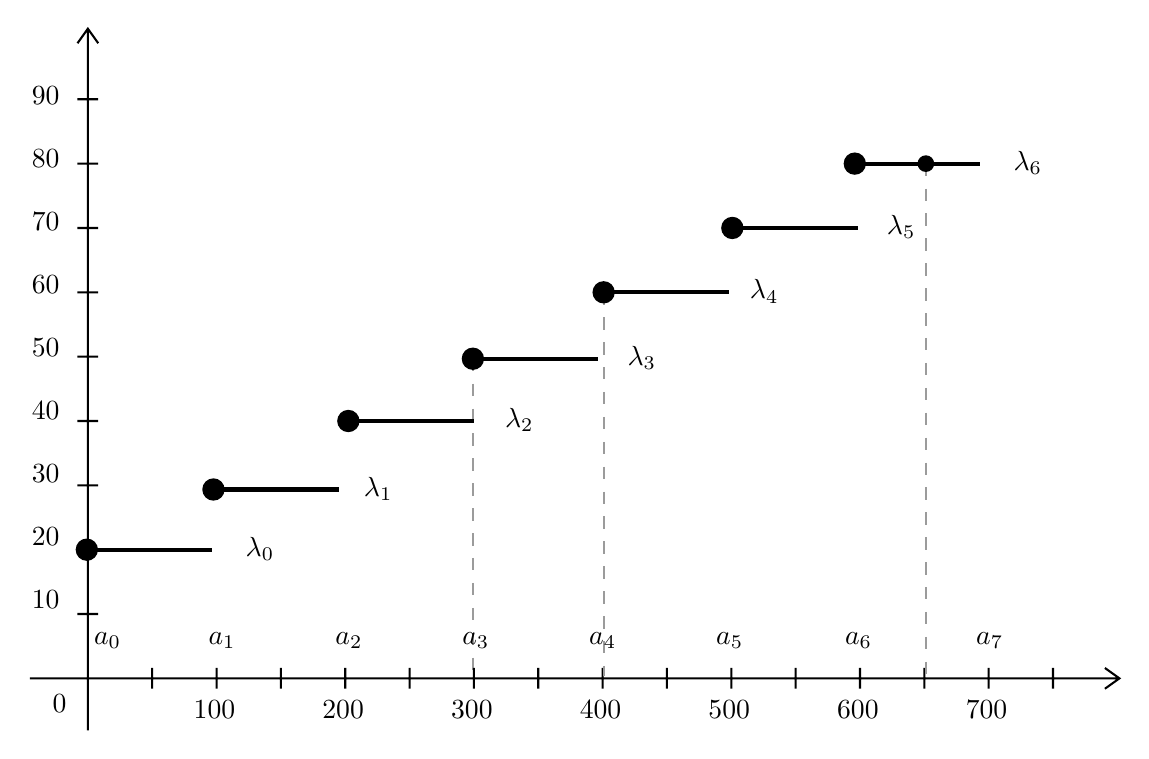
\begin{tikzpicture}[x=0.75pt,y=0.75pt,yscale=-1,xscale=1]
				%uncomment if require: \path (0,1215); %set diagram left start at 0, and has height of 1215
				
				%Straight Lines [id:da4068203359465212] 
				\draw [color={rgb, 255:red, 155; green, 155; blue, 155 }  ,draw opacity=1 ] [dash pattern={on 4.5pt off 4.5pt}]  (295,187) -- (295,339) ;
				%Shape: Axis 2D [id:dp10800599157993496] 
				\draw  (81.5,341) -- (606.5,341)(109.5,28) -- (109.5,366) (599.5,336) -- (606.5,341) -- (599.5,346) (104.5,35) -- (109.5,28) -- (114.5,35) (140.5,336) -- (140.5,346)(171.5,336) -- (171.5,346)(202.5,336) -- (202.5,346)(233.5,336) -- (233.5,346)(264.5,336) -- (264.5,346)(295.5,336) -- (295.5,346)(326.5,336) -- (326.5,346)(357.5,336) -- (357.5,346)(388.5,336) -- (388.5,346)(419.5,336) -- (419.5,346)(450.5,336) -- (450.5,346)(481.5,336) -- (481.5,346)(512.5,336) -- (512.5,346)(543.5,336) -- (543.5,346)(574.5,336) -- (574.5,346)(104.5,310) -- (114.5,310)(104.5,279) -- (114.5,279)(104.5,248) -- (114.5,248)(104.5,217) -- (114.5,217)(104.5,186) -- (114.5,186)(104.5,155) -- (114.5,155)(104.5,124) -- (114.5,124)(104.5,93) -- (114.5,93)(104.5,62) -- (114.5,62) ;
				\draw   ;
				%Straight Lines [id:da2804123014730313] 
				\draw [line width=1.5]    (109,279) -- (169.5,279) ;
				\draw [shift={(109,279)}, rotate = 0] [color={rgb, 255:red, 0; green, 0; blue, 0 }  ][fill={rgb, 255:red, 0; green, 0; blue, 0 }  ][line width=1.5]      (0, 0) circle [x radius= 4.36, y radius= 4.36]   ;
				%Straight Lines [id:da2805363049391225] 
				\draw [line width=1.5]    (170,250) -- (230.5,250) ;
				\draw [shift={(170,250)}, rotate = 0] [color={rgb, 255:red, 0; green, 0; blue, 0 }  ][fill={rgb, 255:red, 0; green, 0; blue, 0 }  ][line width=1.5]      (0, 0) circle [x radius= 4.36, y radius= 4.36]   ;
				%Straight Lines [id:da8418037802662939] 
				\draw [line width=1.5]    (235,217) -- (295.5,217) ;
				\draw [shift={(235,217)}, rotate = 0] [color={rgb, 255:red, 0; green, 0; blue, 0 }  ][fill={rgb, 255:red, 0; green, 0; blue, 0 }  ][line width=1.5]      (0, 0) circle [x radius= 4.36, y radius= 4.36]   ;
				%Straight Lines [id:da33546017232663417] 
				\draw [line width=1.5]    (295,187) -- (355.5,187) ;
				\draw [shift={(295,187)}, rotate = 0] [color={rgb, 255:red, 0; green, 0; blue, 0 }  ][fill={rgb, 255:red, 0; green, 0; blue, 0 }  ][line width=1.5]      (0, 0) circle [x radius= 4.36, y radius= 4.36]   ;
				%Straight Lines [id:da546419164233366] 
				\draw [line width=1.5]    (420,124) -- (480.5,124) ;
				\draw [shift={(420,124)}, rotate = 0] [color={rgb, 255:red, 0; green, 0; blue, 0 }  ][fill={rgb, 255:red, 0; green, 0; blue, 0 }  ][line width=1.5]      (0, 0) circle [x radius= 4.36, y radius= 4.36]   ;
				%Straight Lines [id:da21469695036949776] 
				\draw [line width=1.5]    (479,93) -- (539.5,93) ;
				\draw [shift={(479,93)}, rotate = 0] [color={rgb, 255:red, 0; green, 0; blue, 0 }  ][fill={rgb, 255:red, 0; green, 0; blue, 0 }  ][line width=1.5]      (0, 0) circle [x radius= 4.36, y radius= 4.36]   ;
				%Straight Lines [id:da5930555876339074] 
				\draw [color={rgb, 255:red, 155; green, 155; blue, 155 }  ,draw opacity=1 ] [dash pattern={on 4.5pt off 4.5pt}]  (358,155) -- (358,340) ;
				%Straight Lines [id:da8108696289309665] 
				\draw [line width=1.5]    (358,155) -- (418.5,155) ;
				\draw [shift={(358,155)}, rotate = 0] [color={rgb, 255:red, 0; green, 0; blue, 0 }  ][fill={rgb, 255:red, 0; green, 0; blue, 0 }  ][line width=1.5]      (0, 0) circle [x radius= 4.36, y radius= 4.36]   ;
				%Straight Lines [id:da02236735468995743] 
				\draw [color={rgb, 255:red, 155; green, 155; blue, 155 }  ,draw opacity=1 ] [dash pattern={on 4.5pt off 4.5pt}]  (513.25,93) -- (513.25,341) ;
				%Shape: Circle [id:dp45507800807896026] 
				\draw  [fill={rgb, 255:red, 0; green, 0; blue, 0 }  ,fill opacity=1 ] (509.75,93) .. controls (509.75,91.07) and (511.32,89.5) .. (513.25,89.5) .. controls (515.18,89.5) and (516.75,91.07) .. (516.75,93) .. controls (516.75,94.93) and (515.18,96.5) .. (513.25,96.5) .. controls (511.32,96.5) and (509.75,94.93) .. (509.75,93) -- cycle ;
				
				% Text Node
				\draw (81,54.4) node [anchor=north west][inner sep=0.75pt]    {$90$};
				% Text Node
				\draw (81,84.78) node [anchor=north west][inner sep=0.75pt]    {$80$};
				% Text Node
				\draw (81,115.16) node [anchor=north west][inner sep=0.75pt]    {$70$};
				% Text Node
				\draw (81,145.54) node [anchor=north west][inner sep=0.75pt]    {$60$};
				% Text Node
				\draw (81,175.92) node [anchor=north west][inner sep=0.75pt]    {$50$};
				% Text Node
				\draw (81,206.3) node [anchor=north west][inner sep=0.75pt]    {$40$};
				% Text Node
				\draw (81,236.68) node [anchor=north west][inner sep=0.75pt]    {$30$};
				% Text Node
				\draw (81,267.06) node [anchor=north west][inner sep=0.75pt]    {$20$};
				% Text Node
				\draw (81,297.4) node [anchor=north west][inner sep=0.75pt]    {$10$};
				% Text Node
				\draw (91,347.4) node [anchor=north west][inner sep=0.75pt]    {$0$};
				% Text Node
				\draw (159,350.4) node [anchor=north west][inner sep=0.75pt]    {$100$};
				% Text Node
				\draw (221,350.4) node [anchor=north west][inner sep=0.75pt]    {$200$};
				% Text Node
				\draw (283,350.4) node [anchor=north west][inner sep=0.75pt]    {$300$};
				% Text Node
				\draw (345,350.4) node [anchor=north west][inner sep=0.75pt]    {$400$};
				% Text Node
				\draw (407,350.4) node [anchor=north west][inner sep=0.75pt]    {$500$};
				% Text Node
				\draw (469,350.4) node [anchor=north west][inner sep=0.75pt]    {$600$};
				% Text Node
				\draw (531,350.4) node [anchor=north west][inner sep=0.75pt]    {$700$};
				% Text Node
				\draw (111,317.4) node [anchor=north west][inner sep=0.75pt]    {$a_{0}$};
				% Text Node
				\draw (166.14,317.4) node [anchor=north west][inner sep=0.75pt]    {$a_{1}$};
				% Text Node
				\draw (227.28,317.4) node [anchor=north west][inner sep=0.75pt]    {$a_{2}$};
				% Text Node
				\draw (288.42,317.4) node [anchor=north west][inner sep=0.75pt]    {$a_{3}$};
				% Text Node
				\draw (349.56,317.4) node [anchor=north west][inner sep=0.75pt]    {$a_{4}$};
				% Text Node
				\draw (410.7,317.4) node [anchor=north west][inner sep=0.75pt]    {$a_{5}$};
				% Text Node
				\draw (472.84,317.4) node [anchor=north west][inner sep=0.75pt]    {$a_{6}$};
				% Text Node
				\draw (536,317.4) node [anchor=north west][inner sep=0.75pt]    {$a_{7}$};
				% Text Node
				\draw (184,271.4) node [anchor=north west][inner sep=0.75pt]    {$\lambda _{0}$};
				% Text Node
				\draw (241,242.4) node [anchor=north west][inner sep=0.75pt]    {$\lambda _{1}$};
				% Text Node
				\draw (309,209.4) node [anchor=north west][inner sep=0.75pt]    {$\lambda _{2}$};
				% Text Node
				\draw (368,179.4) node [anchor=north west][inner sep=0.75pt]    {$\lambda _{3}$};
				% Text Node
				\draw (427,147.4) node [anchor=north west][inner sep=0.75pt]    {$\lambda _{4}$};
				% Text Node
				\draw (493,116.4) node [anchor=north west][inner sep=0.75pt]    {$\lambda _{5}$};
				% Text Node
				\draw (554,85.4) node [anchor=north west][inner sep=0.75pt]    {$\lambda _{6}$};
				\end{tikzpicture}
				\vspace*{3mm}
				\caption{Example of a step function}
			\end{figure} 
			Such functions can be found in signal processing and also in statistics for survival analysis.
		\end{itemize}
	\end{enumerate}
	However, there are a very large number of other elementary functions that will meet in the individual sections of this book. Examples include the "Bessel functions" (\SeeChapter{see section Sequences and Series page \pageref{bessel functions}}), the "Lipschitz functions" (\SeeChapter{see section Topology page \pageref{lipschitz functions}}), the "Dirac functions" (\SeeChapter{see section Differential and Integral Calculus page \pageref{dirac function}}), the "distribution functions" (\SeeChapter{see section Statistics page \pageref{distribution function}}), the "Euler gamma function" (\SeeChapter{see section Differential and Integral Calculus page \pageref{gamma euler function}}), etc. The reader will notice that the Dirac function also belongs to the family of distribution functions.
	
	Here is a quite good summary of most elementary functions (non exhaustive but still good!):
	\begin{table}[H]
		\centering
		\begin{tabular}{|c|c|c|c|}
		\hline
		\begin{tikzpicture}[scale=0.45]
		  \begin{axis} [axis lines=center,
		  title={{\LARGE Constant}},
		  xmin=-3,xmax=3,
    	  ymin=-3,ymax=3,
    	  ytick={-3,-2,...,3}]
		    \addplot [domain=-3:3, blue, smooth, thick] { 2 };
		  \end{axis}
		\end{tikzpicture} &
		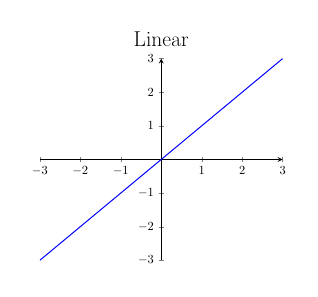
\begin{tikzpicture}[scale=0.45]
		  \begin{axis} [axis lines=center,
		  title={\LARGE Linear},
		  xmin=-3,xmax=3,
    	  ymin=-3,ymax=3,
    	  ytick={-3,-2,...,3}]
		    \addplot [domain=-3:3, blue, smooth, thick] { x };
		  \end{axis}
		\end{tikzpicture} & 
		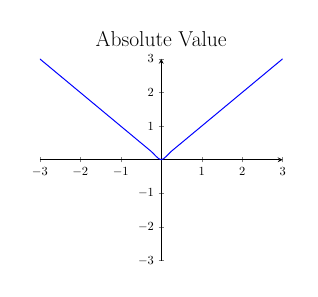
\begin{tikzpicture}[scale=0.45]
		  \begin{axis} [axis lines=center,
		  title={\LARGE Absolute Value},
		  xmin=-3,xmax=3,
    	  ymin=-3,ymax=3,
    	  ytick={-3,-2,...,3}]
		    \addplot [domain=-3:3, blue, smooth, thick] { abs(x) };
		  \end{axis}
		\end{tikzpicture} & 
		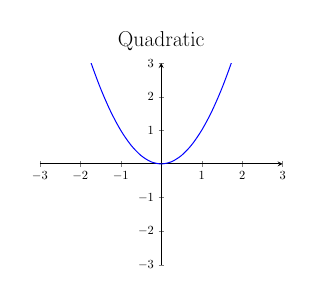
\begin{tikzpicture}[scale=0.45]
		  \begin{axis} [axis lines=center,
		  title={{\LARGE Quadratic}},
		  xmin=-3,xmax=3,
    	  ymin=-3,ymax=3,
    	  ytick={-3,-2,...,3}]
		    \addplot [domain=-3:3, blue, smooth, thick] { x^2 };
		  \end{axis}
		\end{tikzpicture} \\
		$f(x)=c^{te}$ & $f(x)=x$ & $f(x)=|x|$ & $f(x)=x^2$\\ \hline
		\begin{tikzpicture}[scale=0.45]
		  \begin{axis} [axis lines=center,
		  title={{\LARGE Square root}},
		  xmin=-3,xmax=3,
    	  ymin=-3,ymax=3,
    	  ytick={-3,-2,...,3}]
		    \addplot [domain=-3:3, blue, samples=200, smooth, thick] { sqrt(x) };
		  \end{axis}
		\end{tikzpicture} & \begin{tikzpicture}[scale=0.45]
		  \begin{axis} [axis lines=center,
		  title={{\LARGE Cubic}},
		  xmin=-3,xmax=3,
    	  ymin=-3,ymax=3,
    	  ytick={-3,-2,...,3}]
		    \addplot [domain=-3:3, blue, samples=200, smooth, thick] { x^3 };
		  \end{axis}
		\end{tikzpicture} & \begin{tikzpicture}[scale=0.45]
		  \begin{axis} [axis lines=center,
		  title={{\LARGE Cube root}},
		  xmin=-3,xmax=3,
    	  ymin=-3,ymax=3,
    	  ytick={-3,-2,...,3}]
		    \addplot [domain=-3:3, blue, samples=200, smooth, thick] { x^(2/3) };
		  \end{axis}
		\end{tikzpicture} & 
		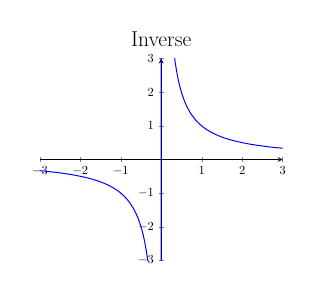
\begin{tikzpicture}[scale=0.45]
		  \begin{axis} [axis lines=center,
		  title={{\LARGE Inverse}},
		  xmin=-3,xmax=3,
    	  ymin=-3,ymax=3,
    	  ytick={-3,-2,...,3}]
		    \addplot [domain=-3:3, blue, samples=200, smooth, thick] { 1/x };
		  \end{axis}
		\end{tikzpicture} \\
		$f(x)=\sqrt{x}$ & $f(x)=x^3$ & $f(x)=\sqrt[3]{x}$ & $f(x)=\dfrac{1}{x}$\\ \hline
		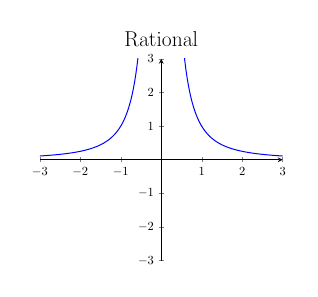
\begin{tikzpicture}[scale=0.45]
		  \begin{axis} [axis lines=center,
		  title={{\LARGE Rational}},
		  xmin=-3,xmax=3,
    	  ymin=-3,ymax=3,
    	  ytick={-3,-2,...,3}]
		    \addplot [domain=-3:-0.1, blue, samples=200, smooth, thick] { 1/x^2 };
		    \addplot [domain=0.1:3, blue, samples=200, smooth, thick] { 1/x^2 };
		  \end{axis}
		\end{tikzpicture}  & 
		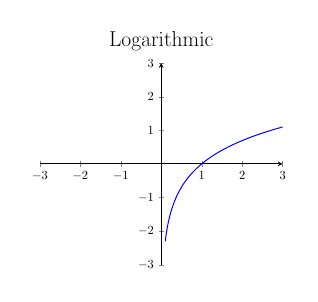
\begin{tikzpicture}[scale=0.45]
		  \begin{axis} [axis lines=center,
		  title={{\LARGE Logarithmic}},
		  xmin=-3,xmax=3,
    	  ymin=-3,ymax=3,
    	  ytick={-3,-2,...,3}]
		    \addplot [domain=0.1:3, blue, samples=200, smooth, thick] { ln(x) };
		  \end{axis}
		\end{tikzpicture}  & 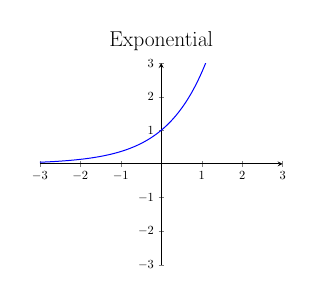
\begin{tikzpicture}[scale=0.45]
		  \begin{axis} [axis lines=center,
		  title={{\LARGE Exponential}},
		  xmin=-3,xmax=3,
    	  ymin=-3,ymax=3,
    	  ytick={-3,-2,...,3}]
		    \addplot [domain=-3:3, blue, samples=200, smooth, thick] { e^x };
		  \end{axis}
		\end{tikzpicture}  & 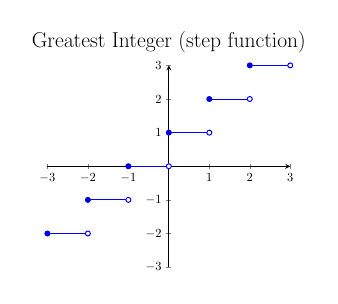
\begin{tikzpicture}[scale=0.45]
		  \begin{axis} [axis lines=center,
		  title={{\LARGE Greatest Integer (step function)}},
		  xmin=-3,xmax=3,
    	  ymin=-3,ymax=3,
    	  ytick={-3,-2,...,3}]
		    \addplot +[thick, samples at={-3,-2,-1,...,2,3},
               jump mark left] {ceil(x+1)};
   			 \addplot  [thick, samples at={-2,-1,0,...,2,3}, only marks,
               mark options={draw=blue,fill=white}] {(x)};
		  \end{axis}
		\end{tikzpicture}  \\
		$f(x)=\dfrac{1}{x^2}$ & $f(x)=\ln(x)$ & $f(x)=e^x$ & $f(x)=[x]$\\ \hline
		\begin{tikzpicture}[scale=0.45]
		  \begin{axis} [axis lines=center,
		  title={{\LARGE Polynomial}},
		  xmin=-3,xmax=3,
    	  ymin=-3,ymax=3,
    	  ytick={-3,-2,...,3}]
		    \addplot [domain=-3:3, blue, samples=200, smooth, thick] { 1/100*(x^6-2*x^5-26*x^4+28*x^3+145*x^2-26*x-80)};
		  \end{axis}
		\end{tikzpicture}  & 
		\begin{tikzpicture}[
		 declare function={binom(\k,\n,\p)=\n!/(\k!*(\n-\k)!)*\p^\k*(1-\p)^(\n-\k);}
		 ,scale=0.45
		]
		\begin{axis}[
			axis lines=center,
			title={{\LARGE Binomial distribution}},
		    samples at={0,...,40},
		    yticklabel style={
		        /pgf/number format/fixed,
		        /pgf/number format/fixed zerofill,
		        /pgf/number format/precision=1
		    }
		]
		\addplot [only marks, blue] {binom(x,40,0.2)};
		\end{axis}
		\end{tikzpicture} & \begin{tikzpicture}[scale=0.45]
			\pgfmathdeclarefunction{gauss}{2}{%
	  		\pgfmathparse{1/(#2*sqrt(2*pi))*exp(-((x-#1)^2)/(2*#2^2))}%
			}
		\begin{axis}[every axis plot post/.append style={
		  samples=50,smooth}, % All plots: from -2:2, 50 samples, smooth, no marks
		  title={{\LARGE Gaussian distribution}},
			  xmin=-3,xmax=3,
	    	  ytick={0,0.1,...,1},
		  enlargelimits=upper,
		  axis lines=center] % extend the axes a bit to the right and top
		  \addplot {gauss(0,1)};
			\end{axis}
			\end{tikzpicture} & \begin{tikzpicture}[scale=0.45]
			\pgfmathdeclarefunction{poiss}{1}{%
			\pgfmathparse{(#1^x)*exp(-#1)/(x!)}%
			}
			\begin{axis}[every axis plot post/.append style={
			  samples at = {0,...,12},
			  axis x line*=bottom,
			  axis y line*=left,
			  enlargelimits=upper},
			  axis lines=center,
			  ytick={0,0.05,...,0.15},
			  title={{\LARGE Poisson distribution}}]
			  \addplot +[ycomb] {poiss(4)};
			\end{axis}
			\end{tikzpicture}  \\
		${\scriptscriptstyle f(x)=1/100(x^6-2x^5-26x^4+\ldots}$ & $f(x)=\mathcal{B}(N,k)$ & $f(x)=e^x$ & $f(x)=\mathcal{P}(\mu,k)$\\ \hline
		\multicolumn{1}{|c|}{\cellcolor[HTML]{EFEFEF}\begin{tabular}[c]{@{}c@{}}Trigonometric\\ Functions\end{tabular}} & \begin{tikzpicture}[scale=0.45]
		  \begin{axis} [axis lines=center,
		  title={{\LARGE Sine}},
		  xmin=-3,xmax=3,
    	  ymin=-3,ymax=3,
    	  ytick={-3,-2,...,3}]
		    \addplot [domain=-3:3, blue, samples=200, smooth, thick] { sin(deg(pi*x)) };
		  \end{axis}
		\end{tikzpicture} & \begin{tikzpicture}[scale=0.45]
		  \begin{axis} [axis lines=center,
		  title={{\LARGE Cosine}},
		  xmin=-3,xmax=3,
    	  ymin=-3,ymax=3,
    	  ytick={-3,-2,...,3}]
		    \addplot [domain=-3:3, blue, samples=200, smooth, thick] { cos(deg(pi*x)) };
		  \end{axis}
		\end{tikzpicture} & \begin{tikzpicture}[scale=0.45]
		\begin{axis}[%
		    axis lines=middle,
		    title={{\LARGE Tangent}},
		    axis on top,
		    xlabel=$x$,
		    ylabel=$y$,
		    domain=-2*pi:2*pi,
		    xmin=-7,
		    xmax=7,
		    ymin=-5,
		    ymax=5,
		    trig format plots=rad, %<- 
		    xtick={-2*pi,-3*pi/2, -pi, -pi/2,pi/2,pi,3*pi/2,2*pi},
		    xticklabels={$-2\pi$, $-\frac{3\pi}{2}$, $-\pi$, $-\frac{\pi}{2}$, $\frac{\pi}{2}$,$\pi$,$\frac{3\pi}{2}$,$2\pi$},
		    every axis y label/.style={rotate=0, black, at={(0.5,1.05)},},
		    every axis x label/.style={rotate=0, black, at={(1.05,0.5)},},,
		    font=\footnotesize,     
		 ]
		\pgfplotsinvokeforeach{-5,-3,...,3}{
		\pgfmathsetmacro{\xmin}{ifthenelse(#1==-5,-2*pi,#1*pi/2+0.01)}
		\pgfmathsetmacro{\xmax}{ifthenelse(#1==3,2*pi,#1*pi/2+pi-0.01)}
		\addplot[samples=51,smooth,blue,domain=\xmin:\xmax]{tan(x)};
		\draw[densely dotted] (#1*pi/2,\pgfkeysvalueof{/pgfplots/ymin})
		 -- (#1*pi/2,\pgfkeysvalueof{/pgfplots/ymax});
		}
		\end{axis}
		\end{tikzpicture} \\ 
		\cellcolor[HTML]{EFEFEF} $\rightarrow$ & $f(x)=\sin(x)$ & $f(x)=\cos(x)$ & $f(x)=\tan(x)$
		\\ \hline
		\end{tabular}
		\caption{A summary of some elementary college level functions}
	\end{table}
	If once you see the plot like that one of an elliptic curve (mathematical tool used in cryptography):
	\begin{figure}[H]
		\centering
		\includegraphics{img/analysis/elliptic_curve.pdf}
	\end{figure}
	You have to avoid to name that a "function". Indeed, by definition, a "function" has to pass the "\NewTerm{vertical line test}\index{vertical line test}": The vertical line test is a method that is used to determine whether a given relation is a function or not. The approach is rather simple. Draw a vertical line cutting through the graph of a relation, and then observe the points of intersections. The vertical line test supports the definition of a function. That is, every $x$-value of a function must be paired to a single $y$-value. If a vertical line intersects the graph of a relation at exactly one point, it implies that a single $x$-value is only paired to a unique value of $y$.
	
	The definition of an "\NewTerm{elliptic curve}\index{elliptic curve}" is the set of all points such that $y^2=x^3+a x+b$. That is, $E_{a, b, c} \equiv\left\{(x, y): y^2=x^3+a x+b\right\}$.
	
	Let a solution $\left(x_0, y_0\right) \in E_{a, b, c}$. then by definition $y_0^2=x_0^3+a x_0+b$. So, $\left(-y_0\right)^2=y_0^2=x_0^3+a x_0+b$. Therefore, $\left(x_0,-y_0\right) \in E_{a, b, c}$. Hence, this will fail the vertical line test at $x=x_0$.

	That is to say, an elliptic curve cannot be a function!
	
	The graph of relation $y R x\Leftrightarrow y^2=x^3-x$ above (as we can't use the word "function" in this case...) is said to be "disconnected"; more specifically, it consists of two "connected components". This is a general topological concept that can be applied to all sets, not just to graphs of relations.
	
	\pagebreak
	\subsubsection{Limits and Continuity of functions}\label{limits}
	We will now consider ordered variables of a special type, which we define by the relation "the variable tends to a limit." In what will follow, the concept of limit of a variable will play a fundamental role, being intimately related to the basic notions of mathematical analysis, derivatives, integrals, etc.
	
	\textbf{Definition (\#\thesection.\mydef):} The number $a$ is named the "\NewTerm{limit}\index{limit}" of variable magnitude $x$, if for any arbitrarily small positive number $\varepsilon$ we have:
	
	If the number $a$ is the limit of the variable $x$, we say that "\NewTerm{$x$ tends to the limit $a$}".

	We can also define the concept of limit from geometrical considerations (this can help to better understand ... but not always ...):
	
	The constant number $a$ is the limit of the variable $x$, if for any given neighbourhood, no matter how small, of center $a$ and of radius $\varepsilon$, we can find a value $x$ such that all the points corresponding to the following values of the variable belong to this neighbourhood (notions that we defined earlier). We represent geometrically this as:
	\begin{figure}[H]
		\centering
		\begin{tikzpicture}[x=0.75pt,y=0.75pt,yscale=-1,xscale=1]
		%uncomment if require: \path (0,436); %set diagram left start at 0, and has height of 436
		
		%Straight Lines [id:da7309089965726057] 
		\draw    (145,130) -- (499.3,130) ;
		\draw [shift={(501.3,130)}, rotate = 180] [color={rgb, 255:red, 0; green, 0; blue, 0 }  ][line width=0.75]    (10.93,-3.29) .. controls (6.95,-1.4) and (3.31,-0.3) .. (0,0) .. controls (3.31,0.3) and (6.95,1.4) .. (10.93,3.29)   ;
		%Straight Lines [id:da09439979422737799] 
		\draw    (154,123) -- (154,138) ;
		%Straight Lines [id:da5228872916751901] 
		\draw    (258,123) -- (258,138) ;
		%Straight Lines [id:da9140904454585459] 
		\draw    (275,123) -- (275,138) ;
		%Straight Lines [id:da04528954434397092] 
		\draw    (351,123) -- (351,138) ;
		%Straight Lines [id:da3104338874710544] 
		\draw    (475,123) -- (475,138) ;
		%Straight Lines [id:da21838175464994203] 
		\draw    (348.3,167) -- (282.3,167) ;
		\draw [shift={(279.3,167)}, rotate = 360] [fill={rgb, 255:red, 0; green, 0; blue, 0 }  ][line width=0.08]  [draw opacity=0] (10.72,-5.15) -- (0,0) -- (10.72,5.15) -- (7.12,0) -- cycle    ;
		\draw [shift={(351.3,167)}, rotate = 180] [fill={rgb, 255:red, 0; green, 0; blue, 0 }  ][line width=0.08]  [draw opacity=0] (10.72,-5.15) -- (0,0) -- (10.72,5.15) -- (7.12,0) -- cycle    ;
		%Straight Lines [id:da04279726467778522] 
		\draw    (471.3,100) -- (261.3,100) ;
		\draw [shift={(258.3,100)}, rotate = 360] [fill={rgb, 255:red, 0; green, 0; blue, 0 }  ][line width=0.08]  [draw opacity=0] (10.72,-5.15) -- (0,0) -- (10.72,5.15) -- (7.12,0) -- cycle    ;
		\draw [shift={(474.3,100)}, rotate = 180] [fill={rgb, 255:red, 0; green, 0; blue, 0 }  ][line width=0.08]  [draw opacity=0] (10.72,-5.15) -- (0,0) -- (10.72,5.15) -- (7.12,0) -- cycle    ;
		
		% Text Node
		\draw (147,140.4) node [anchor=north west][inner sep=0.75pt]    {$0$};
		% Text Node
		\draw (270,140.4) node [anchor=north west][inner sep=0.75pt]    {$x$};
		% Text Node
		\draw (346,140.4) node [anchor=north west][inner sep=0.75pt]    {$a$};
		% Text Node
		\draw (291,172.4) node [anchor=north west][inner sep=0.75pt]    {$| x-a| $};
		% Text Node
		\draw (355,80.4) node [anchor=north west][inner sep=0.75pt]    {$2\varepsilon $};
		
		\end{tikzpicture}
		\vspace*{3mm}
		\caption{Geometric concept of limit in $\mathbb{R}^3$}
	\end{figure}
	\begin{tcolorbox}[title=Remarks,arc=10pt,breakable,drop lifted shadow,
  skin=enhanced,
  skin first is subskin of={enhancedfirst}{arc=10pt,no shadow},
  skin middle is subskin of={enhancedmiddle}{arc=10pt,no shadow},
  skin last is subskin of={enhancedlast}{drop lifted shadow}]
	\textbf{R1.} It should be trivial that the limit of a constant value is equal to this constant, since the inequality $|x-c^{te}|=|c^{te}-c^{te}|=0<\varepsilon $ is always satisfied for an arbitrary $\varepsilon>0$.\\
	
	\textbf{R2.} Not all variable have limits. For example $y=\sin(x)$ as this trigonometric function fluctuates between $[-1,+1]$ from $[-\infty,+\infty]$.
	\end{tcolorbox}
	
	\textbf{Definition (\#\thesection.\mydef):} A variable $x$ tends to infinity if for any positive chosen $M$, we indicate one value of $x$ from which all successive values of the variable $x$ (values in the neighbourhood of the previous chosen value) satisfy the inequality $|x|>M$. Formally:
	
	\begin{itemize}
		\item A variable $x$ "\NewTerm{tends to $+\infty$}" if for any positive chosen $M>0$, we indicate one value of $x$ from which all the successive values of the variables $x$ satisfy the inequality $M<x$.
	
		It is typically the type of consideration that we have for divergent sequences (divergent to infinity) where for a given term of value $M$ of the sequence all the other terms are greater than $M$:
		
		
		\item A variable $x$ "\NewTerm{tends to $-\infty$}" if for any negative chosen $M<0$, we indicate one value of $x$ from which all the successive values of the variable $x$ satisfy the inequality $x<M$:
		
	\end{itemize}
	\textbf{Definition (\#\thesection.\mydef):} Given $y=f(x)$ a function defined in a neighbourhood of $a$ or on some point of this neighbourhood. The function $y=f(x)$ tends to the limit $L$ (that is to say $y\rightarrow L$) when $x$ tends to $a$ (that is to say $x\rightarrow a$) if for any positive number $\varepsilon$ as small as possible, we can indicate a positive number $\delta$ such that all $x$ different from $a$ satisfying the inequality $0<|x-L|<\delta$ also satisfy $|f(x)-L|<\varepsilon$. Formally a function has a limit $L$ on $L$ when in a domain $E$ if:
	
	The relation above is named the "\NewTerm{epsilon-delta definition of limit}\index{epsilon-delta definition of limit} or "\NewTerm{$(\varepsilon,\delta)$ definition of limit}\index{$(\varepsilon,\delta)$ definition of limit}".
	
	The inequality $0<|x-a|<\delta$ gives the possibility to have the distance from which we come with our $x$ without taking care of the direction (left or right) as we take for measurement of distance the absolute values. Indeed on a system of axis representing ordinates values, we can, for a given value, coming from the left or from the right (if necessary you can imagine a bus coming to a bus stop that can from the left or from the right only since the absolute distance from it to the bus stop is less than or equal to $\delta$).
	
	If $L$ is the limit of the function $f(x)$ when $x\rightarrow a$ we then write in this book in any case:
	
	Obviously the above definition is available when $a=\pm \infty$ or/and $L=\pm \infty$!	
	
	To define the direction from which we come from by applying the limit, we use a special notation (recall that this will give us the information of which side of the road comes our bus from...). Thus, if $f(x)$ tends towards the limit $L_1$ when $x$ approaches a number $a$ by taking only values smaller than $a$, then we write:
	
	(notice the small $-$ subscript) and we name $L_1$ the "\NewTerm{left limit}\index{left limit}" of the function $f(x)$ at point $a$ (because remember that the horizontal axis goes from left to right from $-\infty$ to $+\infty$, so small values compared to a given value, are on the left).
	
	If $x$ takes values greater than $a$, then we will write:
	
	(notice the small $+$ subscript) and we name $L_2$ the "\NewTerm{right limit}\index{right limit}" of the function $f(x)$ at point $a$.
	
	In the figure below we have for example: 
	
	\begin{figure}[H]
		\centering
		\begin{tikzpicture}[scale=1.5]
		\begin{axis}[
		  axis lines=middle,
		  samples=200,
		  tick label style={font=\tiny},
		  xtick={-3,...,6},
		  ytick={-3,...,9}
		]
		\addplot[blue,domain=-3:1.85] {1/(x-2) +3 };
		\addplot[blue,domain=2.15:6] {1/(x-2) + 3};
		\draw[red!20,dashed] (axis cs:2,-4) -- (axis cs:2,10);
		\draw[red!20,dashed] (axis cs:-3,3) -- (axis cs:6,3);
		\end{axis}
		\end{tikzpicture}
		\vspace*{3mm}
		\caption{Left and right limit examples}
	\end{figure}
	It is not always easy (or even possible) to calculate limits of some functions. Let us see some typical examples:
	\begin{tcolorbox}[colframe=black,colback=white,sharp corners,breakable]
	\textbf{{\Large \ding{45}}Examples:}\\\\
	E1. Let us prove that:
		
	is true. For this purpose we have to prove that for any small $\varepsilon$ the inequality:
	
	will be satisfied as soon as $|x|>M$ where $M$ is defined by the choice of $\varepsilon$. The previous inequality is obviously equal to:
	
	which is satisfied if we have $x$:
	
	We admit that the example and the method can be discussed.... But in fact it is only an application of the l'Hôpital's rule (ratio of the derivatives) already proved in the section of Differential and Integral Calculus at page \pageref{Hospital rule}. The reader must also know that we will see also other techniques to determine limits further below with better examples.\\
	
	E2. Now using Taylor series and change of variables consider we want to calculate:
	
	The method is quite intuitive. Indeed, first we do a change of variable:
	
	Now consider the Taylor series about $x=0$ for the function $f(x)=\sqrt{1+ax}$. We have:
	
	Which gives:
	
	as a Taylor expansion about $x=0$. Applying this to our limit we see that:
	
	E3. We want to calculate the limit of:
	
	How can we deal with something like this? An idea is the to remember that it also implicitly means:
	
	Hence:
	
	And to answer what is the value of $\theta$, we refer to the plot of the function $\tan(\theta)$ and we see then that the first corresponding value is $\pi/2$, therefore:
	
	\end{tcolorbox}
	
	The signification of the symbols $x\rightarrow -\infty$ and $x\rightarrow +\infty$ makes obvious the signification of the expressions:
	
	and:
	
	that we denote formally by:	
	
	We have defined the case where the function $f(x)$ tends to a certain limit $L$ when $x\rightarrow a_{+,-}$ or $x\rightarrow \pm \infty$. Now let us consider the case where the function tend to infinity when the variable $x$ change in a certain way.
	
	We then have typically and obviously:
	
	Or when we need to indicate the direction:
	
	If the function $f(x) \rightarrow +\infty$ when $a \rightarrow +\infty$ then we write:
	
	And as we have four possibilities for the sign, we write:
	
	that is to say the four following possibilities:
	
	And once again don't forget as we already mentioned before that some function such as for example $f(x)=\sin(x)$ don't have any finite limit when $x\rightarrow \pm \infty$. Then we say that the function is just "bounded" (\SeeChapter{see section Set Theory page \pageref{closed bounded interval}}).
	\begin{figure}[H]
		\centering
		\includegraphics{img/analysis/limite_delucq.jpg}
	\end{figure}
	Now that we've roughly an overview of the concept of limit, we will give an extremely important definition that has a very important place of many areas of high-level mathematics, theoretical physics and computing science (numerical methods). 
	
	\textbf{Definition (\#\thesection.\mydef):} Given a function $f(x)$ and one of its subdomain (or whole one) $E$ (most of time $E \subseteq \mathbb{R}$) and $x_0\in E$, we say that we have a "\NewTerm{continuous function}\index{continuous function}" on $x_0$ if and only if:
	
	That is to say more formally (you have to be able to read the fact that we are going close in an infinitely small way of a limit and this allows the continuity):
	
	named the "\NewTerm{epsilon-delta continuity}\index{epsilon-delta continuity}" or "\NewTerm{$(\varepsilon,\delta)$ continuity}\index{$(\varepsilon,\delta)$ continuity}".
	
	Remember that $|x-x_0|<\delta \Rightarrow |f(x)-f(x_0)|<\varepsilon$ says when the distance of the input relative to $x_0$ is small, the distance of the output relative to $f\left(x_0\right)$ must be small. How small? Arbitrarily small! If $|a-b|<\varepsilon$ for all $\varepsilon>0$, then $a=b$ ! The only way $\left|x-x_0\right|$ can be small is if $x$ was actually really close to $x_0$. That is the purpose of $\delta$! To measure how close we are to $x_0$. So when we move close to $x_0$, we should expect to move closer to $f\left(x_0\right)$ !
	
	In other words: a function is "continuous" if for every point $x_0$ in the domain $E$, we can make the images of that point ($f(x_0)$) and another point ($f(x)$) arbitrarily close (of a distance $\varepsilon$) if we move the other point ($x$) close enough (distance $\delta$) to our given point ($x_0$).
	
	\begin{tcolorbox}[enhanced,colback=red!5!white,colframe=black!50!red,boxrule=1pt,arc=0pt,outer arc=0pt,drop lifted shadow,after skip=10pt plus 2pt]
		\bcbombe Caution! Some people have trouble understanding the difference between the definition of a limit of a function and definition of continuity. The difference is that for the limit $0<|x-L|<\delta$ means that we are not imposing any conditions on the function for $x=L$, while in the definition of continuity, we have $|x-x_0|<\delta$. The difference is that in the definition of continuity at $x_0$, we insist that the function also be defined at $x=x_0$, but we don't in the definition of limit!
		\end{tcolorbox}
	
	The latter relation will be generalized a little bit in the section of Topology and completed with the concept of... "uniform continuity" (that can itself be generlazied by "absolute continuity" but that's out of the scope of this book)!
	
	\begin{figure}[H]
		\centering
		\begin{tikzpicture}[x=0.75pt,y=0.75pt,yscale=-1,xscale=1]
		%uncomment if require: \path (0,428); %set diagram left start at 0, and has height of 428
		
		%Shape: Ellipse [id:dp3142241450603751] 
		\draw  [fill={rgb, 255:red, 248; green, 231; blue, 28 }  ,fill opacity=1 ] (193,125.64) .. controls (193,75.58) and (251.51,35) .. (323.68,35) .. controls (395.86,35) and (454.37,75.58) .. (454.37,125.64) .. controls (454.37,175.7) and (395.86,216.28) .. (323.68,216.28) .. controls (251.51,216.28) and (193,175.7) .. (193,125.64) -- cycle ;
		%Shape: Ellipse [id:dp9358494519007317] 
		\draw  [fill={rgb, 255:red, 208; green, 2; blue, 27 }  ,fill opacity=1 ] (212,140.78) .. controls (212,101.84) and (262.23,70.28) .. (324.18,70.28) .. controls (386.14,70.28) and (436.37,101.84) .. (436.37,140.78) .. controls (436.37,179.71) and (386.14,211.28) .. (324.18,211.28) .. controls (262.23,211.28) and (212,179.71) .. (212,140.78) -- cycle ;
		%Shape: Ellipse [id:dp7086055874904562] 
		\draw  [fill={rgb, 255:red, 126; green, 211; blue, 33 }  ,fill opacity=1 ] (233,155.28) .. controls (233,126.56) and (273.82,103.28) .. (324.18,103.28) .. controls (374.54,103.28) and (415.37,126.56) .. (415.37,155.28) .. controls (415.37,184) and (374.54,207.28) .. (324.18,207.28) .. controls (273.82,207.28) and (233,184) .. (233,155.28) -- cycle ;
		%Shape: Ellipse [id:dp31344736814308494] 
		\draw  [fill={rgb, 255:red, 74; green, 144; blue, 226 }  ,fill opacity=1 ] (249,173.53) .. controls (249,157.1) and (282.66,143.78) .. (324.18,143.78) .. controls (365.71,143.78) and (399.37,157.1) .. (399.37,173.53) .. controls (399.37,189.96) and (365.71,203.28) .. (324.18,203.28) .. controls (282.66,203.28) and (249,189.96) .. (249,173.53) -- cycle ;
		
		% Text Node
		\draw (290,49) node [anchor=north west][inner sep=0.75pt]  [font=\small] [align=left] {Limit Exist};
		% Text Node
		\draw (284,80) node [anchor=north west][inner sep=0.75pt]  [font=\small] [align=left] {Continuous};
		% Text Node
		\draw (257,121) node [anchor=north west][inner sep=0.75pt]  [font=\small] [align=left] {Uniformly Continuous};
		% Text Node
		\draw (256,163) node [anchor=north west][inner sep=0.75pt]  [font=\small] [align=left] {Absolutely Continuous};
		\end{tikzpicture}
	\end{figure}
	
	\begin{tcolorbox}[title=Remarks,arc=10pt,breakable,drop lifted shadow,
  skin=enhanced,
  skin first is subskin of={enhancedfirst}{arc=10pt,no shadow},
  skin middle is subskin of={enhancedmiddle}{arc=10pt,no shadow},
  skin last is subskin of={enhancedlast}{drop lifted shadow}]
	\textbf{R1. }$f$ is "\NewTerm{continuous on the left}\index{continuous on the left}" or respectively "\NewTerm{continuous on the right}\index{continuous on the right}", if we add to the definition above the condition $x>x_0$, respectively $x<x_0$.\\
	
	\textbf{R2.} A continuous function with a continuous inverse function is named a "\NewTerm{homeomorphism}\index{homeomorphism}".\\
	
	\textbf{R3.} Instead of saying when it is necessary that a function is not continuous on $x_0$ or on a given domain, some practitioners prefer to say that the function has an "\NewTerm{oscillation}\index{oscillation}".
	\end{tcolorbox}	
	We have the following trivial corollaries:
	\begin{enumerate}
		\item[C1.] $f(x)$ is continuous on $x_0$ if and only if $f(x)$ is continuous on the left and on the right of $x_0$.
		
		\item[C2.] $f(x)$ is continuous on $E$ if and only if $f(x)$ is continuous on any point of $E$.
	\end{enumerate}
	Let $f(x)$ and $g(x)$ be two functions that are continuous at $x_0$, then we have the following properties (we will prove some of them only on readers requests!):
	\begin{enumerate}
		\item[P1.] $f(x)+g(x)$ (also denoted $(f+g)(x)$) is also epsilon-delta  continuous at $x_0$.
		
		As a reader requested the proof of that claim, let's do it!
		
		If $f(x)$ and $g(x)$ are epsilon-delta continuous at $a$, then $(f+q)(x)$ (shortcut notation for $f(g)+g(x)$) is also epsilon-delta continuous at $a$. 
	 
		 So far a given $\varepsilon>0$ we have to found $\delta>0$ so if $0|x-a|<\delta$, then $|(f+q)(x)-(f+g)(a)|<\varepsilon$.
		 
		First we have obviously:
		
		But because of the triangle inequality of absolute value we have:
		
		As $f(x)$ and $g(x)$ are assumed epsilon-delta continuous, ie $|f(x)-f(a)|<\varepsilon$ when $<|x-a|<\delta_f$ and $|g(x)-f(a)|<\varepsilon$ when $|x-a|<\delta_g$ we have therefore for the previous relation:
		
		Ok you have understand so far how we get that last relation and especially the $2\varepsilon$, let us now reverse the reasoning! We have from the latter:
		
		and let $\delta_h$ be defined as $\min \left(\delta_g, \delta_f\right)$ and $h(x)$ be defined as $f(x)+g(x)$. Therefore:
		
		We can obviously replace $\delta_f$ and $\delta_g$ by $\delta_h$ to get:
		
		Since: 
		
		that we have derived just before is true when $0<|x-a|<\delta_h$, we can find a $\delta_h$ for every value of $2 \varepsilon$.
		
		Finally that means that for every $2 \varepsilon>0$ there is a $\delta>0$ such that $|x-a|<\delta \Longrightarrow|h(x)-h(a)|<2 \varepsilon$ and for every $2 \varepsilon$ there exists an $\varepsilon$ so for every $\varepsilon$ there exists a $\delta$.
		
		\item[P2.] $f(x)-g(x)$ (also denoted $(f-g)(x)$) is also epsilon-delta continuous at $x_0$.
		
		The proof is immediate from the previous proof as we just have to put $-g(x)=h(x)$ (we will admit that the negative sign of a epsilon-delta continuous function is still epsilon-delta continuous without proof) and therefore we fall back on a sum $f(x)+h(x)$.
		
		\item[P3.] $c^{te} f(x)$ is also epsilon-delta continuous at $x_0$.
		
		\item[P4.] $f(x)\cdot g(x)$ (also denoted $fg(x)$) is also epsilon-delta continuous at $x_0$.
		
		Let $f, g: \mathbb{R} \mapsto \mathbb{R}$ be given such that $f$ and $g$ are epsilon-delta continuous. Let $u: \mathbb{R} \mapsto \mathbb{R}$ be defined by $u(x)=f(x) g(x)$. We want to show: $u$ is epsilon-delta continuous, that is, for all $x_0 \in \mathbb{R}$, for every $\varepsilon>0$, there exists some $\delta>0$ such that for all $x \in \mathbb{R}$ with $|x-x_0|<\delta$, $|u(x)-u(x_0)|<\varepsilon$.
	
		We have first using a firs time the properties of the triangle inequality and of the  multiplicativeness of the absolute value:
		
		Now the $\left|f(x)-f\left(x_0\right)\right|$ and $\left|g(x)-g\left(x_0\right)\right|$ terms are good, since $f(x)$ and $g(x)$ are  epsilon-delta continuous at $x_0$. Moreover, the $\left|g\left(x_0\right)\right|$ term is good since it is constant!
		
		The problem is $g(x)$. Let's see if we can do something clever to get rid of it?! We can try to rewrite is using the triangular inequality (again...) of the absolute value:
		
		Now remember that $g(x)$ is continuous, therefore $\forall x \in \mathbb{R} \text { with }|x-x_0|<\delta$ we have:
		
		Therefore we can rewrite the prior-previous inequality as:
		
		So we get finally a relationship that may help us to get rid of the $g(x)$ that mades us problem earlier:
		
		And we can inject it in the step that was making us troubles, that is:
		
		ie:
		
		But as $f(x)$ and $g(x)$ are epsilon-delta continuous we know that we have $\varepsilon_f,\varepsilon_g$ that exist such that:
		
		Therefore:
		
		We may stop here and the proof is finished as we have only constant terms that can be infinitely small. However mathematicians like to finish\footnote{There is a deep reason for that! If we can't finish the proof that way the function will be sure "continuous" but not "uniform continuous" (that's a property most engineers don't care about). For example $x^2$ or $e^x$ are two functions that are epsilon-delta continuous but not uniform continuous. The impact is out of the scope of this book dedicated for reminder to engineers.} the proof with only one term on the right hand side of the equality that looks like a single $\varepsilon$. So obviously as we have two terms that adds together we should have something that looks like $\varepsilon/2+\varepsilon/2=\varepsilon$. For that purpose, mathematicians get rid of the ugly $(\left|g\left(x_0\right)\right|+\varepsilon_g)\cdot\varepsilon_f$ by defining (they absolutely can its not forbidden):
		
		Therefore we have:
		
		Ok it looks better however for mathematicians its still ugly because of the term $|f(x_0)| \cdot \varepsilon_g$. So you may thing we should simple put:
		
		and it's done as the sum of the two terms would give $\varepsilon$! But it's not!!! Because if in the special case where we may have $|f(x_0)|=0$ then we would have a division by zero! So an idea would be to add a value, that we will denote $\Delta\neq 0$ such that the denominator can never be zero. Let us put for example:
		
		However if we do that we don't have:
		
		We see obviously that the only solution to get the expected (pretty) result would be to add a term in the firs factor such that:
		
		However... can we do that? In other words, can we write something like this (if we come some steps backward):
		
		And we see obviously that the answer is YES if and only if $\Delta>0$.
		
		Therefore to summarize all we went through, we have:
		
		And that's the pretty final result mathematicians like to have!
		
		\item[P5.] $|f(x)|$ is also epsilon-delta continuous at $x_0$.
		
		Let $\varepsilon>0$ be given. Then, since $f(x)$ is continuous at $x_0$, there is $\delta>0$ such that if $\left|x-x_0\right|<\delta$, then $\left|f(x)-f\left(x_0\right)\right|<\varepsilon$.
		
		With that same $\delta$, if $\left|x-x_0\right|<\delta$, then by the reverse triangle inequality (\SeeChapter{see section Arithmetic Operators page \pageref{reverse triangle inequality}}), which says $|a-b| \geq|| a|-| b||$, we have:
		
		Therefore $|f(x)|$ is epsilon-delta continuous at $x_0$
		
		\item[P6.] $1/f(x)$ is also epsilon-delta continuous at $x_0$.
		
		This time we need to estimate:
		
		The $\left|f(x)-f\left(x_0\right)\right|$ term is good, and the $\left|f\left(x_0\right)\right|$ term is good as well (since it is constant).
	
		The only term we need to control is the $|f(x)|$ term.
		
		Since we want $\frac{1}{|f(x)|}<$ something, we need $|f(x)|>$ something!
		
		Using the inverse triangular inequality of the absolute value, we know that we have:
		
		But as $|a| \geq-a$ for all $a$, then we can write:
		
		Therefore we get:
		
		But now keep in mind that as $f(x)$ is continuous there is a $\delta_1$ such that if  $\left|x-x_0\right|<\delta_1$, then $\left|f(x)-f\left(x_0\right)\right|<\varepsilon_1$. So let us choose empirically:
		
		Then with this choice (keep in mind that this inequality is valid if and only if $\left|x-x_0\right|$ is small enough and $f(x)\neq 0$ and that we may choose something else than $2$ at the denominator but we made that choice because we will have a nice result at the end!):
		
		And therefore by rearranging:
		
		Hence:
		
		And that good it's want we wanted remember! We wanted $\frac{1}{|f(x)|}<$ something, we needed $|f(x)|>$ something! So now we have it!
		
		Therefore:
		
		So are we stuck? No! Because for the last line above we see that it would be just enough to have:
		
		And this is something we can also choose as $f(x)$ is epsilon-delta continuous and $f(x)\neq 0$.
		
		Therefore we can write the complete proof starting from here now that we have all the tools! :
		
		Let $\varepsilon>0$ be given.
		
		Then, since $f(x)$ is  epsilon-delta continuous at $x_0$, there is $\delta_1>0$ such that if $\left|x-x_0\right|<$ $\delta_1$, then $\left|f(x)-f\left(x_0\right)\right|<\frac{\left|f\left(x_0\right)\right|}{2}$, which implies $|f(x)|>\frac{\left|f\left(x_0\right)\right|}{2}$, and therefore $\frac{1}{|f(x)|}<\frac{2}{\left|f\left(I_0\right)\right|}$.
	
		Moreover, since $f(x)$ is epsilon-delta continuous at $x_0$, there is $\delta_2>0$ such that if $\left|x-x_0\right|<\delta_2$, then $\left|f(x)-f\left(x_0\right)\right|<\frac{\varepsilon}{2}\left|f\left(x_0\right)\right|^2$.
		
		Let $\delta=\min \left\{\delta_1, \delta_2\right\}>0$, then, if $\left|x-x_0\right|<\delta$, then:
			
		And that finish the proof! If $f(x)$ is epsilon-delta continuous then we have indeed $\frac{1}{f}$ that is also epsilon-delta continuous at $x_0$.
		
		\item[P7.] $f(x)/g(x)$ (also denoted $f/g(x)$) is also epsilon-delta continuous at $x_0$.
		
		This is proven immediately using the property of epsilon-delta continuity of the inverse ($1/f(x)$) and of the multiplication  ($f(x)\cdot 1/g(x)$).
		
		\item[P8.] $f^n(x)$ is also epsilon-delta continuous at $x_0$.
		
		This is immediate as it is product $n$ times of $f\cdot f\cdot f\ldots$ as it follows from the property P4.
		
		\item[P9.] $\sqrt[n]{x}$ is also epsilon-delta continuous at $x_0$.
		
		The proof is given in the list of usual limits and continuities further below. What is much more useful is to prove the little bit more general case $\sqrt{f(x)}$ is epsilon-delta continuous!
		
		Suppose you have to prove that $\sqrt{f(x)}$ is a continuous function (where $f(x)$ is continuous). We go by the definition of continuity. Take any $\varepsilon>0$. Then:
		
		Since $f(x)$ should be non-negative:
		
		Since $f(x)$ is continuous we know that there exist a $\delta>0$ such that:
		
		Hence:
		
		and therefore $\sqrt{f(x)}$ is epsilon-delta continuous!
		
		\item[P10.] $g\circ f$ (also denoted $g(f(x))$ is also epsilon-delta continuous at $x_0$.
		
		First a small reminder may be useful!:
		
		If $A, B, C$ are subsets of $\mathbb{R}$ and $f: A \rightarrow B$ and $g: B \rightarrow C$ are functions, then the composition $g \circ f: A \rightarrow C$ is defined by:
		
		Let's show that the composition of two epsilon-delta continuous functions is epsilon-delta continuous! In other words: If $f(x)$ is epsilon-delta continuous at $x_0$ and $g$ is epsilon-delta continuous at $f\left(x_0\right)$, then $g \circ f$ is epsilon-delta continuous at $x_0$.
	
	Let $\varepsilon>0$ be given.
	
	Since $g$ is epsilon-delta continuous at $f\left(x_0\right)$, there is $\delta^{\prime}>0$ such that:
	
	Therefore there is $\delta^{\prime}>0$ such that:
	
	But now, since $f(x)$ is epsilon-delta  continuous at $x_0$, by the definition of epsilon-delta continuity (but with $\delta^{\prime}$ instead of $\varepsilon$), there is $\delta>0$ such that if $\left|x-x_0\right|<\delta$, then $\left|f(x)-f\left(x_0\right)\right|<\delta^{\prime}$.

	Therefore, with $\delta$ as above, if $\left|x-x_0\right|<\delta$, then $\left|f(x)-f\left(x_0\right)\right|<\delta^{\prime}$ and therefore:
	
	Therefore $g \circ f$ is epsilon-delta continuous at $x_0$.

	\end{enumerate}

	\paragraph{Squeeze theorem}\label{Squeeze theorem}\mbox{}\\\\
	The "\NewTerm{squeeze theorem}\index{squeeze theorem}" (also known as the "\NewTerm{sandwich theorem}\index{sandwich theorem}", among other names\footnote{Also known as the pinching theorem, the sandwich rule, the police theorem, the between theorem and sometimes the squeeze lemma. In Italy, the theorem is also known as the theorem of carabinieri.}) is a theorem regarding the limit of a function that is trapped between two other functions.

	The squeeze theorem is used in analysis, typically to confirm the limit of a function via comparison with two other functions whose limits are known. It was first used geometrically by the mathematicians Archimedes and Eudoxus in an effort to compute $\pi$, and was formulated in modern terms by Carl Friedrich Gauss. We will use it further below (in association with the definition of continuity) to compute/prove some very usual limits.
	
	The squeeze theorem is formally stated as follow:
	\begin{theorem}
	Let $I$ be an interval containing the point $a$. Let $g(x), f(x)$, and $h(x)$ be functions defined on $I$, except possibly at $a$ itself. Suppose that for every $x$ in $I$ not equal to $a$, we have:
	
	and also suppose that:
	
	Then:
	
	\begin{figure}[H]
		\centering
		\begin{tikzpicture} 
		\draw[->] (-0.5,0) -- (6,0) node[below] {$x$};
	    \draw[->] (0,-0.5) -- (0,5) node[left] {$y$}; 
	      \draw[red,ultra thick] (-.5,1) to[out=-45,in=185,looseness=2] (4,2) to[out=0,in=135,looseness=1] node [at end,below] {$f$} (6,.5);
	      \draw[blue,ultra thick] (-.5,2.5) to[out=25,in=160,looseness=1] (4,2) to[out=10,in=180,looseness=1] node [at end,above] {$h$} (6,3);
	      \draw[green,ultra thick] (0.5,3.2) to[out=-45,in=175,looseness=1] (4,2) to[out=0,in=180,looseness=1] node [at end,below] {$g$} (6,2.5);
	      \draw[dashed] (4,0) -- node[at start,below] {$a$} (4,2) -- node[at end,left] {$L$} (0,2);
	    \end{tikzpicture}
	\end{figure}
	The functions $g(x)$ and $h(x)$ are said to be lower and upper bounds (respectively) of $f(x)$ and converges to the limit $a$.
	
	 Here, $a$ is not required to lie in the interior of $I$. Indeed, if $a$ is an endpoint of $I$, then the above limits are left- or right-hand limits.
	 
	 \begin{tcolorbox}[enhanced,title=Remark,colframe=black,arc=10pt,drop lifted shadow,after skip=15pt plus 2pt]
	A similar statement holds for infinite intervals: for example, if $I=[0, +\infty[$, then the conclusion holds, taking the limits as $x \rightarrow +\infty$. This theorem is also valid for sequences. Let $\left(a_n\right),\left(c_n\right)$ be two sequences converging to $\ell$, and $\left(b_n\right)$ a sequence. If $\forall n \geq N, N \in \mathbb{N}$ we have $a_n \leq b_n \leq c_n$, then $\left(b_n\right)$ also converges to $\ell$.
	\end{tcolorbox}
	
	
	\end{theorem}
	According to the above hypotheses we have, taking the limit inferior and superior:
	
	so all the inequalities are indeed equalities, and the thesis immediately follows.
	\begin{dem}
	A direct proof, using the $(\varepsilon, \delta)$-definition of limit above, would be to prove that for all real $\varepsilon>0$ there exists a real $\delta> 0$ such that for all $x$ with $|x-a|<\delta$, we have $|f(x)-L|<\varepsilon$. Symbolically:
	
	Let us assume that we know (because it is proven in the context of a special case) that:
	
	This means that:
	
	And let us also assume that we also know (because it is proven in the context of a special case) that:
	
	This means that:
	
	Then we have:
	
	and also:
	
	We can choose $\delta:=\min \left\{\delta_1, \delta_2\right\}$. Then, if $|x-a|<\delta$, combining:
	
	We have:
	
	Hence:
	
	Which completes the proof!
	\begin{flushright}
		$\blacksquare$  Q.E.D.
	\end{flushright}
	\end{dem}
	
	\begin{tcolorbox}[colframe=black,colback=white,sharp corners,breakable]
	\textbf{{\Large \ding{45}}Example:}\\\\
	The limit:
	$$
	\lim _{x \rightarrow 0} x^2 \sin \left(\frac{1}{x}\right)
	$$
	illustrated below:
	\begin{figure}[H]
		\centering
		\begin{tikzpicture}
		\begin{axis}[
		    width=11cm,
		 axis lines=middle,
		 ticklabel style={fill=white},
		 xmin=-1.5,xmax=1.5,
		 ymin=-1.75,ymax=1.75,
		 xlabel=$x$,ylabel=$y$,
		 domain=-1.5:1.5,
		 samples=200,
		 smooth
		        ]
		\addplot[blue] {x*x*sin(4/\x r)};
		\addplot[red] { x*x};
		\addplot[red] {-x*x};
		\end{axis}
		\end{tikzpicture}
	\end{figure}
	Cannot be determined through the limit law:
	$$
	\lim _{x \rightarrow a}(f(x) \cdot g(x))=\lim _{x \rightarrow a} f(x) \cdot \lim _{x \rightarrow a} g(x)
	$$
	because:
	$$
	\lim _{x \rightarrow 0} \sin \left(\frac{1}{x}\right)
	$$
	does not exist.\\
	
	However, by the definition of the sine function:
	$$
	-1 \leq \sin \left(\frac{1}{x}\right) \leq 1
	$$
	It follows that:
	$$
	-x^2 \leq x^2 \sin \left(\frac{1}{x}\right) \leq x^2
	$$
	Since (assuming that its continuity is proven somewhere):
	$$\lim _{x \rightarrow 0}-x^2=\lim _{x \rightarrow 0} x^2=0$$
	by the squeeze theorem, $\lim _{x \rightarrow 0} x^2 \sin \left(\frac{1}{x}\right)$ must also be $0$.
	\end{tcolorbox}
	
	\paragraph{Usual Limits (and Continuities)}\label{Common limits}\mbox{}\\\\
	Delta-epsilon proofs are first found in the works of Augustin-Louis Cauchy (11789–11867 according to holocene calendar).
	
	Here are some usual limits to know (obviously for each of them we will also prove if they are epsilon-delta continuous or not just for curiosity\footnote{Don't forget that the epsilon-delta continuity on a set or subset implies that the limit inside the same set or subset exist too but the contrary is not true!}):
	
	\begin{enumerate}
		\item For any real numbers $a$ and $c$:
		
		
		\begin{itemize}
			\item First we prove the epsilon-delta continuity:
			
			Let us apply the definition of epsilon-delta continuity. We pick an arbitrary real number $x_0$. Then for a given $\varepsilon>0$, we are trying to find a $\delta>0$ such that for all $x$:
			
			Since $0<\varepsilon$ is true by hypothesis, we can choose an arbitrary $\delta$ like $\delta=\pi^{\pi^{\pi^\pi}}$. And this indeed satisfies the condition of epsilon-delta continuity at $x_0$.
			
			Since the choice for $x_0$ was arbitrary, this inequality holds for all real numbers and since the choice for $k$ was arbitrary, this argument holds for all constant functions.
			
			Therefore, all constant functions are epsilon-delta continuous!
			
			\item Second we prove the epsilon-delta limit:
			
			This is by definition. Don't need any proof.
		\end{itemize}
		
		\item For any real number $a$ and $n\in \mathbb{N}^*$:
		
		\begin{itemize}
			\item First we prove the epsilon-delta continuity:
			
			So we have to show $\forall \varepsilon>0$ there is a $\delta>0$ such that:
			
			We have to show that there is a $\delta$ that exists who satisfies the above relation.
			
			Let $\varepsilon$ be any positive number. Denote $x_0+\delta=x$ and $x^n-x_0^n=\Delta$. Then identically:
			
			Taking the absolute value and using its triangle inequality (\SeeChapter{see section Arithmetics page \pageref{absolute value triangle inequality}}) gives:
			
			But since from the triangular inequality $|x|=\left|x_0+\delta\right| \leq \left|x_0\right|+|\delta|$ and also $\left|x_0\right| \leq \left|x_0\right|+|\delta|$, therefore each summand in the parentheses is at most equal to $\left(\left|x_0\right|+|\delta|\right)^{n-1}$, and since there are $n$ summands, the sum is at most equal to $n\left(\left|x_0\right|+|\delta|\right)^{n-1}$. Thus we get:
			
			We may choose $|\delta|<1$. This implies:
			
			The right hand side of this inequality is less than $\varepsilon$ as soon as we still require:
			
			As we are able to found a $\delta$ means that the power function $x \mapsto x^n$ is epsilon-delta continuous at the point $x_0$ (however as the final relation depends on $x_0$ notice that it means the function is not uniform continuous!).
			
			\item Second we prove the epsilon-delta limit:
			
			The proof of the epsilon-delta limit is straightforward thanks to the previous result.
			
			As $x_0=a$, we have:
			
			And therefore we can always found a given $\varepsilon$ such that the above inequality is satisfied and the limit exist on $a$. Then we can indeed write:
			
			Or here is another more detailed argument for those who prefer it:
			
			Let:
			$$x^{\prime}=\frac{x}{x_0}, \delta^{\prime}=\frac{\delta}{x_0}, \varepsilon^{\prime}=\frac{\varepsilon}{x_0^p}$$
			Therefore:
			
			It is obvious to see that, we only need to put:
			
			 in order the rightmost part of the final step to be satisfied. Therefore the epsilon-delta limit is proved to exist!
			
		\end{itemize}
		
		\item For any real number $a>0$:
		
		
		
		\begin{itemize}
			\item First we prove the epsilon-delta continuity:
			
			A function is epsilon-delta continuous at $x_0$ if, for any $\varepsilon>0$, there exists a $\delta>0$ so that, if $|x-x_0|<\delta$, then $|f(x)-f(x_0)|<\varepsilon$.
			
			Therefore:
			
			Thus, if we choose: 
			
			then:
			
			By the way that proves that if $f(x)>0$ is epsilon-delta continuous, then $\sqrt[n]{f(x)}$ is also epsilon-delta continuous!
			
			If you are not convinced of the last claim there is another way to show that! Further below we will prove in details that the exponential function $e^x$ and logarithm function $\log(x)$ are both epsilon-delta continuous. And as we can write:
			
			and we have proven earlier that if $f(x),g(x)$ are both epsilon-delta continuous then $g(f(x))$ is epsilon-delta continuous, then:
			
			is epsilon-delta continuous too! And obviously we can replace $x$ by a epsilon-delta continuous function $f(x)$ and the same reasoning would apply.
			
			\item Second we prove the epsilon-delta limit:
			
			Set $x_n=a^{1 / n}$. We have:
			
			Clearly, we have:
			
			Hence:
			
			which translates into:
			
		\end{itemize}
		
		\item For any real numbers $a$ and $n$:
		

		\begin{itemize}
			\item First we prove the epsilon-delta continuity:
			
			We have already proved earlier that if $f(x)$ is epsilon-delta continuous then $f^n(x)$ is epsilon-delta continuous and also that $a^n$ is therefore also epsilon-delta continuous. 
			
			We also have proven earlier that if $f(x),g(x)$ are epsilon-delta continuous then $f(x)-g(x)$ is also epsilon-delta continuous. Therefore we know that $x^n-a^n$ and $x-a$ are epsilon-delta continuous.
			
			We also have proven earlier that if $f(x),g(x)$ are epsilon-delta continuous then $f(x)/g(x)$ is also epsilon-delta continuous if $g(x)\neq 0$. Therefore we know that:
			
			is epsilon-delta continuous!
			
			\item Second we prove the epsilon-delta limit:
			
			We simply use l'Hôpital's rule (\SeeChapter{see section Differential and Integral Calculus page \pageref{Hospital rule}})! That is:
			
		\end{itemize}
		
		\item For $a>0$ and $n$ positive integer:
		
		
		\begin{itemize}
			\item First we prove the epsilon-delta continuity:
			
			The proof is straightforward as it is just the inverse of the previous example!
			
			\item Second we prove the epsilon-delta limit:
			
			It's just the inverse of the previous example so there is nothing special to prove!
		\end{itemize}
		
		\item We have:
		
		
		\begin{itemize}
			\item First we prove the epsilon-delta continuity:
			
			We have already proved earlier that a constant is epsilon-delta continuous and $x$ is also epsilon-delta continuous.
			
			We have also proved earlier that if $f(x),g(x)$ are epsilon-delta continuous then $f(x)+g(x)$ is epsilon-delta continuous and therefore $1+x$ is epsilon-delta continuous.
			
			We have also proved earlier that if $f(x)>0$ is epsilon-delta continuous that $f(x)^{1/x}$ is also epsilon-delta continuous. Therefore:
			
			is epsilon-delta continuous!
			
			
			\item Second we prove the epsilon-delta limit:
			
			This limit is already proven at page \pageref{Euler number}.
			
		\end{itemize}
		
		\item For any real number $a$ \label{definition exponential function}:
		
		
		This limit is well known by students in the special case where $a=1$.
		
		\begin{itemize}
			\item First we prove the epsilon-delta continuity:
			
			We have already proved earlier that a constant is epsilon-delta continuous. Therefore $1$ is epsilon-delta continuous.
			
			We have also proved earlier that if $f(x),g(x)\neq 0$ are epsilon-delta continuous then $f(x)/g(x)$ is also epsilon-delta continuous and therefore $a/x$ is epsilon-delta continuous.
			
			We have also proved earlier that if $f(x),g(x)$ are epsilon-delta continuous then $f(x)+g(x)$ is epsilon-delta continuous and therefore $1+(a/x)$ is  epsilon-delta continuous.
			
			We have also proved earlier that if $f(x)$ is epsilon-delta continuous that $f(x)^{n}$ is also epsilon-delta continuous. Therefore:
			
			is epsilon-delta continuous!
			
			\item Second we prove the epsilon-delta limit:
			
			 Let us note that it is equivalent to show that:
			
			Do not worry about the domain of $\ln$, since for large $n$, the expression $1+\frac{a}{n}$ will be a positive number (close to $1$). Consider the function:
			
			and $f(0)=1$. Using the definition of the derivative of $\ln(1+x)$, we see that $f(x)$ is epsilon-delta continuous at $0$, that is, $\lim _{x \rightarrow 0} f(x)=1=f(0)$. Hence, for any sequence $\left\{x_n\right\}$ which converges to $0$, we have:
			
			Now, set:
			
			Clearly we have $x_n \rightarrow 0$. Therefore, we have:
			
			But, we have:
			
			which clearly implies:
			
			Since:
			
			we get:
			
		\end{itemize}
		
		\item We have:
		

		\begin{itemize}
			\item First we prove the epsilon-delta continuity:
			
			Suppose $\left|x-x_0\right|<\delta$ and fix $\varepsilon>0$.
			
			Consider $\left|e^x-e^{x_0}\right|<\varepsilon$, then using an engineer approach\footnote{Because for mathematicians this proof, although correct, relies on several facts about the logarithm, which (assuming it is defined as the inverse of the exponential) is usually shown to be a total function using the intermediate value theorem and hence assuming that the exponential is continuous... We also have to be careful with taking logs if $e^{x_0}-\varepsilon<0$...}:
			
			Hence $e^x$ is epsilon-delta continuous at $x_0$ as long as:
			
			Since $x_0$ is arbitrarily chosen then $e^x$ is epsilon-delta continuous and we are done.
			
			Now that we have proven that the exponential is epsilon-delta continuous. We know that the numerator is epsilon-delta continuous and also that the denominator is epsilon-delta continuous. As we have proven earlier that if $f(x)$ and $g(x)$ are epsilon-delta continuous, then $f(x)/g(x)$ is epsilon-delta continuous too, this finish the proof!
			
			\item Second we prove the epsilon-delta limit:
			
			That latter is immediate using l'Hôpital's rule (\SeeChapter{see section Differential and Integral Calculus page \pageref{Hospital rule}})! We have indeed:
			
			
		\end{itemize}
		
		\item We have :
		
		
		This limit must not be confused with the Maclaurin series that gives for small $x$ that $\sin(x)\cong x$.
		
		\begin{itemize}
			\item First we prove the epsilon-delta continuity:
			
			Let $\varepsilon>0$ and $x, y \in \mathbb{R}$. We want:
			
			Using trigonometric identities this is equivalent to:
			
			Because $| \cos (\alpha)| \leqslant 1, \forall \alpha \in \mathbb{R}$ we can simplify:
			
			it suffices:
			
			when:
			
			Since $|\sin (x)| \leq|x|$:
			
			Choosing $\delta=\varepsilon/2>0$ will do the trick. Because $\delta$ doesn't depend on $x, y$, the continuity is uniform!
			
			\item Second we prove the epsilon-delta limit:
			
			If we use the analytical definition of the $\sin(x)$ function (power series):
			
			Therefore calculating:
			
			is equivalent to:
			
			And we have already proven earlier before that:
			
			Therefore:
			
			Hence:
			
		\end{itemize}
		
		\item We have:
		
		
		The method will be exactly similar to that of $\sin(x)$ seen just earlier!
		
		\begin{itemize}
			\item First we prove the epsilon-delta continuity:
			
			Let $\varepsilon>0$ and $x, y \in \mathbb{R}$. We want:
			
			Using trigonometric identities this is equivalent to:
			
			Because $| \sin(\alpha)| \leqslant 1, \forall \alpha \in \mathbb{R}$ we can simplify:
			
			it suffices:
			
			when:
			
			Since $|\sin (x)| \leq|x|$:
			
			Choosing $\delta=\varepsilon/2>0$ will do the trick. Because $\delta$ doesn't depend on $x, y$, the continuity is uniform.
			
			\item Second we prove the epsilon-delta limit:
			
			If we use the analytical definition of the $\cos(x)$ function (power series):
			
			Therefore calculating:
			
			is equivalent to:
			
			And we have already proven earlier before that:
			
			Therefore:
			
			Hence:
			
		\end{itemize}
		
		\item We have:
		
		
		\begin{itemize}
			\item First we prove the epsilon-delta continuity:
			
			The proof is straightforward! As by definition:
			
			He have proved earlier that $\sin(x)$ but also $\cos(x)$ are epsilon-delta continuous.
			
			But we have also proved that if $f(x),g(x)\neq 0$ are epsilon-delta continuous then $f(x)/g(x)$ is epsilon-delta continuous. 
			
			Therefore $\tan(x)$ is epsilon-delta continuous!
			
			\item Second we prove the epsilon-delta limit:
			
			Notice that by the geometric definition we have:
			
			And we have proved earlier above:
			
			Therefore:
			
		\end{itemize}
		
		\item We have:
		
		There are multiple ways more or less rigorous to prove that limit (geometric based, derivation based, series based, numerical based, squeeze theorem based, l'Hôpital theorem based, etc.) and that depend also on the definition of the function $\sin(x)$ itself...
		\begin{itemize}
			\item First we prove the epsilon-delta continuity:
			
			We have proven earlier that $\sin(x)$ is epsilon-delta continuous and also that $x$ is epsilon-delta continuous. And we have proven earlier in the general case that if $f(x),g(x)$ are epsilon-delta continuous functions, assuming $g(x)\neq 0$, then $f(x)/g(x)$ is also epsilon-delta continuous!
			
			So that finish our proof!
			
			\item Second we prove the epsilon-delta limit:
			
			We have:
			
			if and only if for every $\varepsilon>0$, there exists a $\delta>0$ such that $|f(x)-1|<\varepsilon$ whenever $0<|x-0|<\delta$.

			Let $\varepsilon>0$ be an arbitrary real number.
			
			Note that:
			
			If $x \neq 0$, we have:
			
			We thus have:
			
			Therefore we have:
			
			If $0<|x|<1$, then $0<\left|x^2\right|<1$, and the infinite series $\sum_{n=1}^{+\infty}\left|x^2\right|^n$ converges to $\frac{x^2}{1-x^2}$.
			
			Choose $\delta:=\sqrt{\frac{\varepsilon}{1+\varepsilon}}$. Then $0<|x-0|<\delta$ implies that $0<|x|<\sqrt{\frac{\varepsilon}{1+\varepsilon}}<1$, and hence $x^2<\varepsilon-\varepsilon x^2$. But $x^2<\varepsilon-\varepsilon x^2$ implies that $\frac{x^2}{1-x^2}<\varepsilon$.
			
			We therefore have $\sum_{n=1}^{+\infty}\left|x^2\right|^n<\varepsilon$ whenever $0<|x-0|<\delta$. But since $|f(x)-1| \leq \sum_{n=1}^{+\infty}\left|x^2\right|^n$, we have $|f(x)-1|<\varepsilon$ whenever $0<|x-0|<\delta$.
			
			Since $\varepsilon$ was arbitrary, we have: 
			
			
		\end{itemize}
		
		\item We have:
		
		
		\begin{itemize}
			\item First we prove the epsilon-delta continuity:
			
			Let us put $z=1+x$ and we want to prove the epsilon-delta continuity near $x_0=0$ hence near $\log_b(1)$ for $b>1$.
			
			Let $\varepsilon>0$ and $z_0>0$. We want to find a small enough $\delta$ such that for $\left|z-z_0\right|<\delta$, $\left|\log_b(z)-\log_b\left(z_0\right)\right|<\varepsilon$. We have:
			
			What we want is for $z/z_0$ to be close to $1$. A better condition would be:
			
			In that case, we would have, by the strictly increasing nature of the $\log$ function:
			
			Therefore:
			
			So we are able to find such a $\varepsilon$ but we see that the later is dependent of $z_0$ and we can't get rid of the latter. Hence $\log_b(z)$ is epsilon-delta continuous on $z_0$ but not uniformly continuous.
			
			Notice that in the literature it's very common to rearrange:
			
			as following:
			
			and to subtract $z_0$ everywhere such that:
			
			As we wish to have $|z-z_0|<\delta$, he have finally:
			
			When the base is the natural exponential the latter is written:
			
			
			\item Second we prove the epsilon-delta limit:
			
			We simply use l'Hôpital's rule (\SeeChapter{see section Differential and Integral Calculus page \pageref{Hospital rule}})! That is:
			
		\end{itemize}
		
		\item We have:
		
		
		\begin{itemize}
			\item First we prove the epsilon-delta continuity:
			
			Don't try to use the derivative or integral definition of $\arcsin(x)$ as they assume you already know that the function is epsilon-delta continuous! We want here to avoid using the "inverse theorem" as the latter is quite abstract and the proof not yet provided in this book (and very likely will never be!).
			
			The trick will be to used another expression for the $\arcsin(x)$ that uses the continuity proven earlier for $\sin(x)$. Let us remind for that purpose that we have proved in the section Numbers at page \pageref{de Moivre and Euler formulas} the following de Moivre and Euler formula:
			
			Let us put that as equal to $y$ such that:
			
			Hence:
			
			So we just need to solve for $x$. It will be a little bit easier if we do the substitution $e^{\mathrm{i}x}=z$. Therefore we get:
			
			And after rearranging:
			
			We apply the quadratic formula and get:
			
			One solution equals $z$ the other solution equals $1/z$ pick one. And lets reverse the substitution:
			
			Therefore:
			
			So we have finally the interesting substitution:
			
			And we can rewrite our limit as:
			
			So we have to prove that:
			
			is epsilon-delta continuous for $0<x<1$! And now that will be straightforward as we have proven that the sum of two epsilon-delta continuous function is epsilon-delta continuous (the content of the logarithm above). But also that the square root is epsilon-delta continuous (still the content of the logarithm above) and just previously that the logarithm is also epsilon-delta continuous! Hence the whole numerator above is epsilon-delta continuous for $0<x<1$!
			
			And as the denominator ($x$) is also epsilon-delta continuous and that we have proven if $f(x),g(x)\neq 0$ are epsilon-delta continuous then $f(x)/g(x)$ is also epsilon-delta continuous. Then:
			
			is indeed epsilon-delta continuous for $0<x<1$!
						
			\item Second we prove the epsilon-delta limit:
			
			We convert the inverse trigonometric sine function by the mathematical relationship between the trigonometric and inverse trigonometric functions. That is $y=\sin^{-1}(x)$, then $x=\sin(y)$.
			
			Therefore, the quotient of $\arcsin(x)$ by $x$ can be written as the ratio of $y$ to $\sin(y)$ mathematically:
			
			Therefore, if $x$ approaches zero, then $y$ tends to $\sin^{-1}(0)$. More explicitly:
			
		\end{itemize}
		
		\item We have:
		
		
		\begin{itemize}
			\item First we prove the epsilon-delta continuity:
			
			We have already proved earlier that $\tan(x)$ is epsilon-delta continuous and same for $x$.
			
			We have also proved earlier that if $f(x),g(x)\neq 0$ are epsilon-delta continuous then $f(x)/g(x)$ is also epsilon-delta continuous.
			
			Therefore: 
			
			is epsilon-delta continuous!
			
			\item Second we prove the epsilon-delta limit:
			
			Once we have proved:
			
			We can prove quite easily that:
			
			Indeed:
			
		\end{itemize}
		
		\item We have:
		
		
		\begin{itemize}
			\item First we prove the epsilon-delta continuity:
			
			Don't try to use the derivative or integral definition of $\arctan(x)$ as they assume you already know that the function is epsilon-delta continuous! We want here to avoid using the "inverse theorem" as the latter is quite abstract and the proof not yet provided in this book (and very likely will never be!).
			
			The trick will be to used another expression for the $\arctan(x)$ that uses the continuity proven earlier for $\sin(x)$ and $\cos(x)$. Let us remind for that purpose that we have proved in the section Numbers at page \pageref{de Moivre and Euler formulas} the following de Moivre and Euler formula:
			
			which leads to:
			
			Let $\tan (\varphi)=x$, then:
			
			and solving it we find that:
			
			which leads us to:
			
			when $\forall x \in \mathbb{C} \backslash(\mathrm{i}(]-\infty,-1] \cup[1,+\infty[))$.
			
			Therefore we can rewrite the limit above as:
			
			As we have proven that a constant is epsilon-delta continuous and $x$ (and therefore $\mathrm{i}x$) is also epsilon-delta continuous then $1-\mathrm{i}x$ and $1+\mathrm{i}x$ are both epsilon-delta continuous.
			
			But we have also proved earlier above that the logarithm is epsilon-delta continuous. Therefore as we have proven that if $f(x),g(x)$ are epsilon-delta continuous then $g(f(x))$ is also epsilon-delta continuous that lead us to the result that $\ln (1-\mathrm{i}x)$ and $\ln (1+\mathrm{i}x)$ are both epsilon-delta continuous!
			
			As we have also proved that if $f(x),g(x)\neq 0$ are epsilon-delta continuous then $f(x)/g(x)$ is also epsilon-delta continuous then the ratio of of $\ln (1-\mathrm{i}x)-\ln (1+\mathrm{i} x)$ by $x$ is also epsilon-delta continuous.
			
			Finally we have proven that:
			
			is indeed epsilon-delta continuous $\forall x \in \mathbb{C} \backslash(\mathrm{i}(]-\infty,-1] \cup[1,+\infty[))$.
			
			\item Second we prove the epsilon-delta limit:
			
			This is straightforward. Again we just use l'Hospital rule (\SeeChapter{see section Differential and Integral Calculus page \pageref{Hospital rule}}) and this leads to:
			
		\end{itemize}
		
		\item We have:
		
		
		\begin{itemize}
			\item First we prove the epsilon-delta continuity:
			
			This is straightforward to prove! We have proven earlier that a constant (like $1$) is epsilon-delta continuous.
			
			We have also proven that $x$ is epsilon-delta continuous.
			
			We have proven that if $f(x),g(x)$ are epsilon-delta continuous then $f(x)+ g(x)$ and $f(x)-g(x)$ are  also epsilon-delta continuous. 
			
			We have proven earlier that if $f(x)$ is epsilon-delta continuous then $f(x)^n$ is epsilon-delta continuous. Therefore $a^x-1$ is epsilon-delta continuous. 
			
			We have proven that if $f(x),g(x)\neq 0$ are epsilon-delta continuous then $f(x)/g(x)$ is also epsilon-delta continuous.
			
			Therefore:
			
			is epsilon-delta continuous!
			
			\item Second we prove the epsilon-delta limit:
			
			Let $y=a^x-1$, then $1+y=a^x$.
			
			Consider the relation:
			
			Using the logarithm on both sides, we have:
			
			Also:
			
			This shows that $y \rightarrow 0$ as $x \rightarrow 0$. Therefore, the given limit can be written as:
			
			Using the relation $\lim _{x \rightarrow 0}(1+x)^{\frac{1}{x}}=e$, we have:
			
			But $\ln (e)=1$, we have:
			
		\end{itemize}
		
		\item We have:
		
		
		\begin{itemize}
			\item First we prove the epsilon-delta continuity:
			
			This is straightforward to prove! We have proven earlier that a constant (like $1$) is epsilon-delta continuous.
			
			We have also proven that $x$ is epsilon-delta continuous.
			
			We have proven that if $f(x),g(x)$ are epsilon-delta continuous then $f(x)+ g(x)$ and $f(x)-g(x)$ are  also epsilon-delta continuous. Therefore $1+x$ is epsilon-delta continuous.
			
			We have proven earlier that if $f(x)$ is epsilon-delta continuous then $f(x)^n$ is epsilon-delta continuous. Therefore $(1+x)^m-1$ is epsilon-delta continuous.
			
			We have proven that if $f(x),g(x)\neq 0$ are epsilon-delta continuous then $f(x)/g(x)$ is also epsilon-delta continuous. Therefore:
			
			is epsilon-delta continuous!
			
			\item Second we prove the epsilon-delta limit:
			
			This is straightforward. Again we just use l'Hospital rule (\SeeChapter{see section Differential and Integral Calculus page \pageref{Hospital rule}}) and this leads to:
			
		\end{itemize}
		
		\item We have:
		
		
		\begin{itemize}
			\item First we prove the epsilon-delta continuity:
			
			The proof is straightforward! We have already proved earlier that a constant is epsilon-delta continuous therefore $1$ has the same behaviour.
			
			We have already proved also earlier that $\cos(x)$ is epsilon-delta continuous !
			
			And we have proved that $x$ is epsilon-delta continuous.
			
			We have proved that if $f(x),g(x)$ are epsilon-delta continuous then $f(x)-g(x)$ is epsilon-delta continuous. Therefore $1-\cos(x)$ is epsilon-delta continuous.
			
			We have proved that if $f(x),g(x)\neq 0$ are epsilon-delta continuous then $f(x)/g(x)$ is epsilon-delta continuous. Therefore:
			
			is epsilon-delta continuous!
			
			\item Second we prove the epsilon-delta limit:
			
			We have proven earlier above that:
			
			Hence:
			
		\end{itemize}
		
		\item We have:
			
			often denoted:
			
		
		\begin{itemize}
			\item First we prove the epsilon-delta continuity:
			
			The proof is straightforward as:
			
			Indeed, we have proven in the previous examples that for $x>0$, we had $1/x$ and $\ln(x)$ were epsilon-delta continuous.
			
			And as we have proven in the general case that if $f(x),g(x)$ are epsilon-delta continuous then $f(x)\cdot g(x)$ was also epsilon-delta continuous, then $\frac{1}{x} \ln (x)$ is epsilon-delta continuous!
			
			We have also proven in the example above that the exponential $e$ is epsilon-delta continuous. And because we have proven in the general case that if $f(x),g(x)$ are epsilon-delta continuous then $g(f(x))$ is also epsilon-delta continuous, then:
			
			is epsilon-delta continuous and so is $x^{1/x}$ !
			
			\item Second we prove the epsilon-delta limit:
			
			Set $x_n=n^{1 / n}$. We have:
			
			Clearly, we have (from above):
			
			Hence:
			
			which translates into:
			
		\end{itemize}
		
		\item We have:
		
		
		\begin{itemize}
			\item First we prove the epsilon-delta continuity:
			
			The proof is straightforward as we have proven that $\log(x)$ is epsilon-delta continuous (therefore $\ln(x)$ has the same behaviour) and that $x$ is also epsilon-delta continuous.
			
			And we have proved earlier that if $f(x),g(x)$ are epsilon-delta continuous  then $f(x)\cdot g(x)$ is also epsilon-delta continuous.
			
			Hence:
			
			is epsilon-delta continuous!
			
			\item Second we prove the epsilon-delta limit:
			
			If we evaluate the limit of the numerator and denominator separately we'll find that as $\ln (x)$ goes to $+\infty$ as $x$ goes to $+\infty: \ln (+\infty)=+\infty$ and $x$ goes to $+\infty$.
			
			Therefore we have a ratio of two infinities $\frac{+\infty}{+\infty}$ meaning that we will have to apply l'Hôpital's rule (\SeeChapter{see section Differential and Integral Calculus page \pageref{Hospital rule}}):
			
			The limit approaches $0$ because $1$ divided over something approaching $+\infty$ becomes closer and closer to $0$.
		\end{itemize}
		
		\item We have:
		
		
		\begin{itemize}
			\item First we prove the epsilon-delta continuity:
			
			We have already proved earlier that $\log(x)$ is epsilon-delta continuous.
			
			We have also already proved earlier that $x$ is epsilon-delta continuous.
			
			We have proved earlier that if we have $f(x),g(x)\neq 0$ that are epsilon-delta continuous then $f(x)/g(x)$ is epsilon-delta continuous.
		
			Therefore:
			
			is epsilon-delta continuous!
			
			\item Second we prove the epsilon-delta limit:
			
			The proof is straightforward using l'Hôpital's rule (\SeeChapter{see section Differential and Integral Calculus page \pageref{Hospital rule}})! Indeed:
			
			
		\end{itemize}
		
		\item We have:
		
		
		\begin{itemize}
			\item First we prove the epsilon-delta continuity:
			
			The proof follows exactly the same pattern as the case with $x^{1/x}$ done earlier above and leads to the same conclusion: $x^x$ is epsilon-delta continuous for $x>0$.
			
			\item Second we prove the epsilon-delta limit:
			
			The proof uses a result we have obtained in one of the previous example. That is:
			
			How? That's easy! We just rewrite:
			
			And therefore the result is immediate:
			
			
		\end{itemize}
		
		\item We have:
		
		
		\begin{itemize}
			\item First we prove the epsilon-delta continuity:
			
			That will be also straightforward thank to all previous examples!
			
			First we have proven that a constant like $1$ is epsilon-delta continuous.
			
			We have also proven that $\sin(x)$ is epsilon-delta continuous.
			
			We have also proven that in the general case if $f(x),g(x)$ are epsilon-delta continuous then $f(x)+g(x)$ is epsilon-delta continuous. Therefore $1+\sin(x)$ is epsilon-delta continuous.
			
			We have proven earlier that if $x>0$ then $x^{1/x}$ was epsilon-delta continuous. Therefore we conclude (in the engineering way...) that:
			
			is epsilon-delta continuous!
			
			\item Second we prove the epsilon-delta limit:
			
			Here we use exactly the same trick as before...! That is we rewrite the limit as:			
			
			Therefore we just have to compute:
			
			We use l'Hôpital's rule (\SeeChapter{see section Differential and Integral Calculus page \pageref{Hospital rule}})! Therefore we get:
			
			Therefore:
			
		\end{itemize}
		
		\item We have for any real $a$:
		
		
		\begin{itemize}
			\item First we prove the epsilon-delta continuity:
			
			
			The proof is straightforward using again the results of the previous examples and the general properties of epsilon-delta continuity!
			
			Indeed, we have already proven that a constant (like $a$ or like $a^2$ that is still a constant too) is epsilon-delta continuous.
			
			We have also proven earlier above that $x^2$ is epsilon-delta continuous.
			
			And as we have proven the property that if $f(x),g(x)$ are epsilon-delta continuous then $f(x)-g(x)$ is epsilon-delta continuous. That means $x^2-a^2$ is epsilon-delta continuous.
			
			We have proven earlier also that if $f(x)>0$ is epsilon-delta continuous then $\sqrt{f(x)}$ is also epsilon-delta continuous. Therefore for  $x^2-a^2>0$ (i.e. $x^2>a^2$, or $|x|>|a|$), we have that $\sqrt{x^2-a^2}$ is epsilon-delta continuous too!
			
			\item Second we prove the epsilon-delta limit:
			
			We use a trick:
			
			Hence after simplification:
			
			It's obvious now as $x>a$ and therefore that $\sqrt{x^2-a^2}\geq 0$ that:
			
			Hence:
			
		\end{itemize}
		
		
		
		\item We have:
		
		
		\begin{itemize}
			\item First we prove the epsilon-delta continuity:
			
			This is quite straightforward thanks to everything we have proven so far! Indeed, we have proven earlier above that $\tan(x)$ and $\sin(x)$ are epsilon-delta continuous. But we have also proven earlier that if $f(x),g(x)$ are epsilon-delta continuous then $f(x)-g(x)$ is epsilon-delta continuous. Therefore $\tan(x)-\sin(x)$ is  epsilon-delta continuous.
			
			And we have also proven earlier that if $f(x)$ is epsilon-delta continuous then $f(x)^n$ is also epsilon-delta continuous and therefore $x^3$ at the denominator is also epsilon-delta continuous.
			
			And finally as we have proven earlier that if $f(x),g(x)\neq 0$ are epsilon-delta continuous then $f(x)/g(x)$ is also epsilon-delta continuous and therefore:
			
			is epsilon-delta continuous!
			
			\item Second we prove the epsilon-delta limit:
			
			Let us do that without l'Hôpital's rule (personal choice!). So we use the definitions of trigonometric functions:
			
			Using the property that:
			
			We get:
			
		\end{itemize}
		
		\item For $q>0$:
		
		
		\begin{itemize}
			\item First we prove the epsilon-delta continuity:
			
			The proof will be straightforward again thanks to everything we have proven so far! Indeed, we have proven earlier that the logarithm is epsilon-delta continuous, therefore $\log(x)$ is epsilon-delta continuous.
			
			We have also proven that $x$ is epsilon-delta continuous.
			
			We have also proven that if $f(x)$ is an epsilon-delta continuous function then $f^n(x)$ is also epsilon-delta continuous. Hence $\log^p(x)$ and $x^q$ are epsilon-delta continuous.
			
			And finally as we have proven that if $f(x),g(x)\neq 0$ are epsilon-delta continuous then $f(x)/g(x)$ is epsilon-delta continuous that lead us to the conclusion that:
			
			is epsilon-delta continuous!
			
			\item Second we prove the epsilon-delta limit:
			
			We simply use l'Hôpital's rule (\SeeChapter{see section Differential and Integral Calculus page \pageref{Hospital rule}})! That is:
			
		\end{itemize}
		
		\item We have:
		
		This formula is due to the English scientist and mathematician Edmond Halley (11656 to 11742 according to holocene calendar) and was known also by Leonhard Euler, who used it for defining the natural logarithm.
		
		\begin{itemize}
			\item First we prove the epsilon-delta continuity:
			
			The proof is straightforward we everything we have seen so far! Indeed, in the first examples above we have proven that $\sqrt[n]{x}$ is epsilon-delta continuous and also that a constant (like $1$) is also epsilon-delta continuous.
			
			But we have proven earlier that if $f(x),g(x)$ are the both epsilon-delta continuous then $f(x)-g(x)$ is also epsilon-delta continuous. Therefore $\sqrt[n]{x}-1$ is epsilon-delta continuous.
			
			And finally we have proven that if $f(x)$ is epsilon-delta continuous then that same function multiplied by a constant is also epsilon-delta continuous. Therefore:
			
			is epsilon-delta continuous!
			
			\item Second we prove the epsilon-delta limit:
			
			We change the $n$-th root to power of $e$ and use the power series expansion of exponential function:
			
			And finally:
			
		\end{itemize}
		
		\item We want to show if:
		
		There are many ways to handle this sequence. Let us use calculus techniques again. Consider the function:
		
		We have:
		
		and:
		
		for any $n \geq 1$. Note that for any $x \in[n, n+1]$, we have:
		
		hence:
		
		which gives:
		
		Since:
		
		we get:
		
		In particular, we have:
		
		Therefore, since $\lim _{n \rightarrow +\infty} \ln (n+1)=+\infty$, we must have:
		
	\end{enumerate}
	We will stop here the list of common epsilon-delta limits and epsilon-delta continuities as it is almost without end! And the reader must keep in mind that we have focused only on univariate functions here above and that most of the examples were only for real valued functions (only two were in the complex planes)...
	
	Most engineers don't like this topic but don't forget that it's the only rigorous way to show that a function can be differentiate or integrate (among other important application for professional mathematicians and theoretical physicists)!
	
	To summarize here is a table with the most important limits:
	\begin{table}[H]
		\centering
		\begin{tabular}{|l|l|l|}
		\hline
		\multicolumn{3}{|l|}{\cellcolor[HTML]{C0C0C0}\textbf{Most common limits}} \\ \hline
		$\displaystyle\lim _{z \rightarrow a} c^{te}=c^{te}$ & $\displaystyle\lim _{x \rightarrow a} x^n=a^n$ & $\displaystyle\lim _{x \rightarrow 0} x^2 \sin \left(\frac{1}{x}\right)$  \\ \hline
		$\displaystyle\lim _{z \rightarrow+\infty}\left(1+\frac{a}{x}\right)^z=e^a$ & $\displaystyle\lim _{x \rightarrow 0} \frac{e^x-1}{x}=1$ & $\displaystyle\lim _{x \rightarrow 0} \sin (x)=0$   \\ \hline
		$\displaystyle\lim _{x \rightarrow 0} \tan (x)=0$ & $\displaystyle\lim _{z \rightarrow 0}(1+x)^{1 / x}=e$ & $\displaystyle\lim _{x \rightarrow a} \frac{x-a}{x^n-a^n}=\frac{1}{n a^{n-1}}$   \\ \hline
		$\displaystyle\lim _{x \rightarrow 0} \frac{\sin (x)}{x}=1$ & $\displaystyle\lim _{x \rightarrow 0} \frac{\log (1+x)}{x}=1$ & $\displaystyle\lim _{x \rightarrow 0}\frac{\arcsin (x)}{x}=1$   \\ \hline
		$\displaystyle\lim _{z \rightarrow 0} \frac{\arctan (x)}{x}=1$ & $\displaystyle\lim _{z \rightarrow 0} \frac{a^x-1}{x}=\ln (a)$ & $\displaystyle\lim _{x \rightarrow 0} \frac{1-\cos (x)}{x}=0$   \\ \hline
		$\displaystyle\lim _{x \rightarrow 0^{+}} x \ln (x)=0$ & $\displaystyle\lim _{z \rightarrow+\infty} \frac{\ln (x)}{x}=0$ & $\displaystyle\lim _{x \rightarrow 0}(1+\sin (x))^{1 / x}=e$   \\ \hline
		$\displaystyle\lim _{x \rightarrow+\infty} x-\sqrt{x^2-a^2}=0$ & $\displaystyle\lim _{x \rightarrow 0} \frac{\tan (x)-\sin (x)}{x^3}=\frac{1}{2}$ & $\displaystyle\lim _{x \rightarrow+\infty} \frac{\log ^p(x)}{x^q}=0$   \\ \hline
		$\displaystyle\lim _{n \rightarrow+\infty}\left(1+\frac{1}{2}+\frac{1}{3}+\ldots+\frac{1}{n}\right)=+\infty$ & $\displaystyle\lim _{n \rightarrow+\infty} \sqrt[n]{a}=1$ & $\displaystyle\lim _{x \rightarrow 0} \cos (x)=1$  \\ \hline
		$\displaystyle\lim _{x \rightarrow a} \frac{x^n-a^n}{x-a}=n a^{n-1}$ & $\displaystyle\lim _{z \rightarrow 0} \frac{\tan (x)}{x}=1$ & $\displaystyle\lim _{z \rightarrow+\infty} x^{1 / x}=1$  \\ \hline
		$\displaystyle\lim _{x \rightarrow 0} x^x=1$ & $\displaystyle\lim _{z \rightarrow 0} \frac{\tan (x)}{x}=1$ & $\displaystyle\lim _{x \rightarrow+\infty} n(\sqrt[n]{x}-1)=\log (x)$  \\ \hline
		\end{tabular}
		\caption{Most common limits}
	\end{table}
	
	\begin{tcolorbox}[enhanced,title=Remark,colframe=black,arc=10pt,drop lifted shadow,after skip=15pt plus 2pt]
	In some of the proofs of usual limits seen earlier above the reader may have noticed that sometimes that arguments turn out to involve not just $\varepsilon$ but a constant multiple of it. This may occur for instance when the limit involves a sum or several arithmetic processes.\\
	
	But is $K\varepsilon$ just as good as $\varepsilon$? If we en upd with a proof with  $2 \varepsilon$, or $22 \varepsilon$, or $0.001\varepsilon$, that's just as good as coming out with $\varepsilon$! Indeed if $\varepsilon$ is an arbitrary small number, so is $22 \epsilon$ and $0.001\varepsilon$. Therefore, if we can prove something is less than $K \varepsilon$, you have shown that it can be made as small as desired.\\
	
	We formulate this as a general principle, the "\NewTerm{$K$-$\varepsilon$ principle}\index{$K-\varepsilon$ principle}". This isn't a standard term in analysis, so don't use it when you go to your next mathematics congress, but it is useful to name an idea that will recur often.
	\end{tcolorbox}
	
	\paragraph{Limit laws}\mbox{}\\\\
	We now take a look at the "\NewTerm{limit laws}\index{limit laws}", the individual properties limits in the univariate case. The proofs will be omitted as it is quite intuitive but any reader can request us the proof of one of them if needed!
	
	Let $f(x)$ and $g(x)$ be defined for all $x\neq a$ over some open interval containing $a$. Assume that $L$ and $M$ are real numbers such that:
	
	Let $c^{te}$ be a constant. Then, each of the following statements holds:		
	\begin{itemize}
		\item The sum law for limits gives:
		
		
		\item The difference law for limits gives:
		
		
		\item Constant multiple law for limits:
		
		
		\item Product law for limits:
		
		
		\item Quotient law for limits:
		
		for $M\neq 0$.
		
		\item Power law for limits:
		
		for every positive integer $n$.
		
		\item Root law for limits:
		
		for all $L$ if $n$ is odd and for $L\geq 0$ if $n$ is even.
	\end{itemize}
	
	\paragraph{Asymptotes}\mbox{}\\\\
	The term "\NewTerm{asymptote}\index{asymptote}" is used in mathematics to precise possible properties of an infinite branch of curve which growth tends to an infinitesimal value.
	
	In analytic geometry, an asymptote of a curve is simply said to be a line such that the distance between the curve and the line approaches zero as they tend to infinity. In some contexts, such as algebraic geometry, an asymptote is defined as a line which is tangent to a curve at infinity.
	
	The study of asymptotic behavior is particularly developed in the studies of functions. In the scientific field, it is common to study time-dependent functions (evolution of populations, chemical or nuclear reactions, temperature graphs, oscillation of a shock absorber). One of the researcher's objectives is then to know the state at the end of the experiment, that is to say when a large interval of time has passed. The objective is then not to know the intermediate variations, but to determine the stable, infinite behavior of the measured phenomenon. The researcher therefore studies the asymptotic behavior of his function with the tools that mathematics offers him.
	\begin{tcolorbox}[title=Remark,arc=10pt,breakable,drop lifted shadow,
  skin=enhanced,
  skin first is subskin of={enhancedfirst}{arc=10pt,no shadow},
  skin middle is subskin of={enhancedmiddle}{arc=10pt,no shadow},
  skin last is subskin of={enhancedlast}{drop lifted shadow}]
	The word "asymptote" is derived from the Greek and means "not falling together".
	\end{tcolorbox}	
	
	\textbf{Definitions (\#\thesection.\mydef):}
	
	\begin{enumerate}
		\item[D1.] When the limit of a function $f(x)$ tends to a constant 
$c^{te}$ when $x \rightarrow \pm \infty$, then the graphical representation of this function leads us to draw a horizontal line that we name "\NewTerm{horizontal asymptote}\index{horizontal asymptote}" which equation satisfies:
		
		
		\item[D2.] When the limit of a function $f(x)$ tends to $\pm \infty$ when $x \rightarrow a_{+,-}$, then the graphical representation of this function leads us to draw a vertical line that we name "\NewTerm{vertical asymptote}\index{vertical asymptote}" which equation satisfies:
		
		Vertical asymptotes is the typical symptom of a division by zero in a fraction and has a very important place in physics. The syndrome is also named a "\NewTerm{singularity}\index{singularity}".
		\begin{tcolorbox}[colframe=black,colback=white,sharp corners]
		\textbf{{\Large \ding{45}}Example:}\\\\
		The graph of the function:
		
		 has the straight lines of $x=1$ as vertical asymptote and $y=0$ as horizontal asymptote:
		 \begin{figure}[H]
			\centering
			\begin{tikzpicture}[scale=1.5]
			\begin{axis}[
			  axis lines=middle,
			  samples=200,
			  tick label style={font=\tiny},
			  xtick={-2,...,2},
			  ytick={-20,-15,...,20}
			]
			\addplot[blue,domain=-2:0.96] {1/(x-1)};
			\addplot[blue,domain=1.04:2] {1/(x-1)};
			\draw[red!20,dashed] (axis cs:1,-20) -- (axis cs:1,20);
			\end{axis}
			\end{tikzpicture}
			\vspace*{3mm}
			\caption{Graphical representation of a horizontal and vertical asymptote}
		\end{figure}
		\end{tcolorbox}
		
		\item[D3.] The straight line of equation $y=ax+b$ is an "\NewTerm{oblique asymptote}\index{oblique asymptote}" or "\NewTerm{slant asymptote}\index{slant asymptote}" of a curve of function $f(x)$ if:
		
		the values of $a$ and $b$ can be easily found using the following relations:
		
		
		\begin{tcolorbox}[enhanced,colback=red!5!white,colframe=black!50!red,boxrule=1pt,arc=0pt,outer arc=0pt,drop lifted shadow,after skip=10pt plus 2pt]
		\bcbombe Caution! A curve may have two distinct oblique asymptotes in $+\infty$ and $-\infty$.
		\end{tcolorbox}
		
		To find a possible oblique asymptote, one must already be certain that the function $f(x)$ admits an infinite limit in $+\infty$ or $-\infty$ then only we look for the limits at $-\infty$ and $+\infty$ of $f(x)/x$ and $f(x)-ax$.
		
		Three typical cases can be considered for oblique asymptotes:
		\begin{enumerate}
			\item The representative curve of $f(x)$ has for asymptotical direction the affine equation $y=ax$:
			
			\begin{tcolorbox}[colframe=black,colback=white,sharp corners]
			\textbf{{\Large \ding{45}}Example:}\\\\
			The graph of the function:
			
			 has the straight line of $y=x$ as oblique asymptote:
			 \begin{figure}[H]
				\centering
				\begin{tikzpicture}[scale=1.5]
				\begin{axis}[
				  axis lines=middle,
				  samples=200,
				  tick label style={font=\tiny},
				  xtick={-10,-5,...,10},
				  ytick={-20,-5,...,20}
				]
				\addplot[blue,domain=-10:-0.2] {x+1/x};
				\addplot[blue,domain=0.2:10] {x+1/x};
				\draw[red!20,dashed] (axis cs:-10,-10) -- (axis cs:10,10);
				\end{axis}
				\end{tikzpicture}
				\vspace*{3mm}
				\caption{Graphical representation of an oblique affine asymptote}
			\end{figure}
			\end{tcolorbox}
			
			\item The representative curve of $f(x)$ has an infinite branch (this branch has not close form asymptote) and the only one thing we can say is that $x$-axis is the direction of this asymptote. Such an asymptote exists when:
			
			\begin{tcolorbox}[colframe=black,colback=white,sharp corners]
			\textbf{{\Large \ding{45}}Example:}\\\\
			The functions $f(x)=\sqrt{x}$ (in red) or $\ln(x)$ (in green) have a limit $f(x)/x$ equal to $0$ and both have a "parabolic branch" of direction following the $x$-axis:
			 \begin{figure}[H]
				\centering
				\begin{tikzpicture}[scale=1.5]
				\begin{axis}[
				  axis lines=middle,
				  samples=200,
				  tick label style={font=\tiny},
				  xtick={0,5,...,20},
				  ytick={-3,-2,...,3}
				]
				\addplot[red,domain=0.1:20] {x^(1/2)/x};
				\addplot[green,domain=0.3:20] {ln(x)/x};
				%\draw[red!20,dashed] (axis cs:-10,-10) -- (axis cs:10,10);
				\end{axis}
				\end{tikzpicture}
				\vspace*{3mm}
				\caption{Graphical representation of a parabolic branch example following $x$-axis}
			\end{figure}
			\end{tcolorbox}
			
			\item The representative curve of $f(x)$ has an infinite branch (this branch has not close form asymptote) and the only one thing we can say is that $y$-axis is the direction of this asymptote (we then also speak of "parabolic branch"):
			
	
			\item A function $f(x)$ is say to have a "\NewTerm{curvilinear asymptote}\index{curvilinear asymptote}" if it satisfies:
			
			for $n>1$ where for recall $P_n(x)$ is a polynomial of degree $n$.
			\begin{tcolorbox}[colframe=black,colback=white,sharp corners,breakable]
			\textbf{{\Large \ding{45}}Example:}\\\\
			The function :
			
			has a curvilinear asymptote that is:
			
			Indeed:
			
			 \begin{figure}[H]
				\centering
				\begin{tikzpicture}[scale=1.5]
				\begin{axis}[
				  axis lines=middle,
				  samples=200,
				  tick label style={font=\tiny},
				  xtick={-6,-4,...,6},
				  ytick={-30,-20,...,50}
				]
				\addplot[blue,domain=-6:-0.1] {(x^3+2*x^2+3*x+4)/x};
				\addplot[blue,domain=0.1:6] {(x^3+2*x^2+3*x+4)/x};
				\addplot[red!20,dashed,domain=-6:6] {x^2+2*x+3};
				%\draw[red!20,dashed] (axis cs:-10,-10) -- (axis cs:10,10);
				\end{axis}
				\end{tikzpicture}
				\vspace*{3mm}
				\caption[Graphical representation of a curvilinear asymptote]{Graphical representation of a curvilinear asymptote of equation $x^2+2 x+3$}
			\end{figure}
			\end{tcolorbox}
		\end{enumerate}
	\end{enumerate}
	There are many techniques for finding limits that apply in various conditions. It's important to know all these techniques, but it's also important to know when to apply which technique. Some basic techniques who doesn't involve derivation are:
	\begin{figure}[H]
		\centering
		\resizebox{0.73\textwidth}{!}{\begin{tikzpicture}[x=0.75pt,y=0.75pt,yscale=-1,xscale=1]
		%uncomment if require: \path (0,1229); %set diagram left start at 0, and has height of 1229
		
		%Straight Lines [id:da18906794328365484] 
		\draw [color={rgb, 255:red, 248; green, 231; blue, 28 }  ,draw opacity=1 ][line width=1.5]    (296,178) -- (152,178) ;
		%Straight Lines [id:da24063317977376286] 
		\draw [color={rgb, 255:red, 208; green, 2; blue, 27 }  ,draw opacity=1 ][line width=1.5]    (507,178) -- (363,178) ;
		%Straight Lines [id:da913576757436229] 
		\draw [color={rgb, 255:red, 248; green, 231; blue, 28 }  ,draw opacity=1 ][line width=1.5]    (154,215) -- (154,178) ;
		\draw [shift={(154,219)}, rotate = 270] [fill={rgb, 255:red, 248; green, 231; blue, 28 }  ,fill opacity=1 ][line width=0.08]  [draw opacity=0] (11.61,-5.58) -- (0,0) -- (11.61,5.58) -- cycle    ;
		%Straight Lines [id:da8524157097249603] 
		\draw [color={rgb, 255:red, 208; green, 2; blue, 27 }  ,draw opacity=1 ][line width=1.5]    (507,215) -- (507,178) ;
		\draw [shift={(507,219)}, rotate = 270] [fill={rgb, 255:red, 208; green, 2; blue, 27 }  ,fill opacity=1 ][line width=0.08]  [draw opacity=0] (11.61,-5.58) -- (0,0) -- (11.61,5.58) -- cycle    ;
		%Straight Lines [id:da5612605101427182] 
		\draw [color={rgb, 255:red, 126; green, 211; blue, 33 }  ,draw opacity=1 ][line width=1.5]    (329,215) -- (329,198.5) ;
		\draw [shift={(329,219)}, rotate = 270] [fill={rgb, 255:red, 126; green, 211; blue, 33 }  ,fill opacity=1 ][line width=0.08]  [draw opacity=0] (11.61,-5.58) -- (0,0) -- (11.61,5.58) -- cycle    ;
		%Straight Lines [id:da04906264821321682] 
		\draw [color={rgb, 255:red, 208; green, 2; blue, 27 }  ,draw opacity=1 ][line width=1.5]    (508.5,478) -- (508.5,419) ;
		%Straight Lines [id:da7343936463443095] 
		\draw [color={rgb, 255:red, 208; green, 2; blue, 27 }  ,draw opacity=1 ][line width=1.5]    (508.5,477) -- (329,477) ;
		%Straight Lines [id:da013009788077467999] 
		\draw [color={rgb, 255:red, 208; green, 2; blue, 27 }  ,draw opacity=1 ][line width=1.5]    (329,514) -- (329,477) ;
		\draw [shift={(329,518)}, rotate = 270] [fill={rgb, 255:red, 208; green, 2; blue, 27 }  ,fill opacity=1 ][line width=0.08]  [draw opacity=0] (11.61,-5.58) -- (0,0) -- (11.61,5.58) -- cycle    ;
		%Straight Lines [id:da2871938973014796] 
		\draw [color={rgb, 255:red, 74; green, 144; blue, 226 }  ,draw opacity=1 ][line width=1.5]    (329,570) -- (329,545.5) ;
		\draw [shift={(329,574)}, rotate = 270] [fill={rgb, 255:red, 74; green, 144; blue, 226 }  ,fill opacity=1 ][line width=0.08]  [draw opacity=0] (11.61,-5.58) -- (0,0) -- (11.61,5.58) -- cycle    ;
		%Straight Lines [id:da3876588032540529] 
		\draw [color={rgb, 255:red, 189; green, 16; blue, 224 }  ,draw opacity=1 ][line width=1.5]    (178,533) -- (154,533) ;
		%Straight Lines [id:da6059546460523775] 
		\draw [color={rgb, 255:red, 189; green, 16; blue, 224 }  ,draw opacity=1 ][line width=1.5]    (154,570) -- (154,533) ;
		\draw [shift={(154,574)}, rotate = 270] [fill={rgb, 255:red, 189; green, 16; blue, 224 }  ,fill opacity=1 ][line width=0.08]  [draw opacity=0] (11.61,-5.58) -- (0,0) -- (11.61,5.58) -- cycle    ;
		%Straight Lines [id:da3413726374276538] 
		\draw [color={rgb, 255:red, 80; green, 227; blue, 194 }  ,draw opacity=1 ][line width=1.5]    (508.5,533) -- (481,533) ;
		%Straight Lines [id:da793759127137666] 
		\draw [color={rgb, 255:red, 80; green, 227; blue, 194 }  ,draw opacity=1 ][line width=1.5]    (508.5,570) -- (508.5,533) ;
		\draw [shift={(508.5,574)}, rotate = 270] [fill={rgb, 255:red, 80; green, 227; blue, 194 }  ,fill opacity=1 ][line width=0.08]  [draw opacity=0] (11.61,-5.58) -- (0,0) -- (11.61,5.58) -- cycle    ;
		%Straight Lines [id:da9375667994685268] 
		\draw [color={rgb, 255:red, 139; green, 87; blue, 42 }  ,draw opacity=1 ][line width=1.5]    (480.5,524) -- (598.5,524) ;
		%Straight Lines [id:da15764312838320493] 
		\draw [color={rgb, 255:red, 139; green, 87; blue, 42 }  ,draw opacity=1 ][line width=1.5]    (598.5,524) -- (598.5,876) ;
		%Straight Lines [id:da9998514847759088] 
		\draw [color={rgb, 255:red, 0; green, 0; blue, 0 }  ,draw opacity=1 ][line width=1.5]    (154,800) -- (508.5,800) ;
		%Straight Lines [id:da8682805380230487] 
		\draw [color={rgb, 255:red, 139; green, 87; blue, 42 }  ,draw opacity=1 ][line width=1.5]    (434.5,876) -- (598.5,876) ;
		%Straight Lines [id:da7035220946747038] 
		\draw [color={rgb, 255:red, 0; green, 0; blue, 0 }  ,draw opacity=1 ][line width=1.5]    (329,831) -- (329,806.5) ;
		\draw [shift={(329,835)}, rotate = 270] [fill={rgb, 255:red, 0; green, 0; blue, 0 }  ,fill opacity=1 ][line width=0.08]  [draw opacity=0] (11.61,-5.58) -- (0,0) -- (11.61,5.58) -- cycle    ;
		%Straight Lines [id:da5005121602577964] 
		\draw [color={rgb, 255:red, 0; green, 0; blue, 0 }  ,draw opacity=1 ][line width=1.5]    (187,857) -- (66.5,857) ;
		%Straight Lines [id:da09324939036642887] 
		\draw [color={rgb, 255:red, 0; green, 0; blue, 0 }  ,draw opacity=1 ][line width=1.5]    (66.5,121) -- (66.5,857) ;
		%Straight Lines [id:da06966576660078116] 
		\draw [color={rgb, 255:red, 0; green, 0; blue, 0 }  ,draw opacity=1 ][line width=1.5]    (66.5,121) -- (201.5,121) ;
		\draw [shift={(205.5,121)}, rotate = 180] [fill={rgb, 255:red, 0; green, 0; blue, 0 }  ,fill opacity=1 ][line width=0.08]  [draw opacity=0] (11.61,-5.58) -- (0,0) -- (11.61,5.58) -- cycle    ;
		%Straight Lines [id:da9853533477920391] 
		\draw [color={rgb, 255:red, 139; green, 87; blue, 42 }  ,draw opacity=1 ][line width=1.5]    (434.5,913) -- (434.5,876) ;
		\draw [shift={(434.5,917)}, rotate = 270] [fill={rgb, 255:red, 139; green, 87; blue, 42 }  ,fill opacity=1 ][line width=0.08]  [draw opacity=0] (11.61,-5.58) -- (0,0) -- (11.61,5.58) -- cycle    ;
		%Straight Lines [id:da9211902710314455] 
		\draw [color={rgb, 255:red, 155; green, 155; blue, 155 }  ,draw opacity=1 ][line width=1.5]    (90.5,524) -- (178,524) ;
		%Straight Lines [id:da44622818726928526] 
		\draw [color={rgb, 255:red, 155; green, 155; blue, 155 }  ,draw opacity=1 ][line width=1.5]    (90.5,524) -- (90.5,849) ;
		%Straight Lines [id:da56336198170769] 
		\draw [color={rgb, 255:red, 155; green, 155; blue, 155 }  ,draw opacity=1 ][line width=1.5]    (90.5,876) -- (236.5,876) ;
		%Straight Lines [id:da9830418523509263] 
		\draw [color={rgb, 255:red, 155; green, 155; blue, 155 }  ,draw opacity=1 ][line width=1.5]    (236.5,913) -- (236.5,876) ;
		\draw [shift={(236.5,917)}, rotate = 270] [fill={rgb, 255:red, 155; green, 155; blue, 155 }  ,fill opacity=1 ][line width=0.08]  [draw opacity=0] (11.61,-5.58) -- (0,0) -- (11.61,5.58) -- cycle    ;
		%Straight Lines [id:da9391390955150849] 
		\draw [color={rgb, 255:red, 155; green, 155; blue, 155 }  ,draw opacity=1 ][line width=1.5]    (90.5,863) -- (90.5,876) ;
		
		% Text Node
		\draw (207,16) node [anchor=north west][inner sep=0.75pt]  [font=\LARGE] [align=left] {Calculating $\displaystyle \lim _{x\rightarrow 0} f( x)$};
		% Text Node
		\draw (212,108) node [anchor=north west][inner sep=0.75pt]   [align=left] {\begin{minipage}[lt]{180pt}\setlength\topsep{0pt}
		\begin{center}
		\textbf{{\large A. Direct susbstitution}}\\Try to evaluate the function directly
		\end{center}
		
		\end{minipage}};
		% Text Node
		\draw (303.5,161) node [anchor=north west][inner sep=0.75pt]  [font=\LARGE] [align=left] {$\displaystyle f( a)$};
		% Text Node
		\draw (115.5,223) node [anchor=north west][inner sep=0.75pt]  [font=\large] [align=left] {$\displaystyle f( a) =\dfrac{b}{0}$};
		% Text Node
		\draw (293.5,234) node [anchor=north west][inner sep=0.75pt]  [font=\large] [align=left] {$\displaystyle f( a) =b$};
		% Text Node
		\draw (418.5,223) node [anchor=north west][inner sep=0.75pt]  [font=\large] [align=left] {$\displaystyle f( a) =\dfrac{0}{0}$};
		% Text Node
		\draw (89.5,275) node [anchor=north west][inner sep=0.75pt]   [align=left] {where $b$ is not zero};
		% Text Node
		\draw (245.5,275) node [anchor=north west][inner sep=0.75pt]   [align=left] {where $b$ is a real number};
		% Text Node
		\draw (105,300) node [anchor=north west][inner sep=0.75pt]   [align=left] {\begin{minipage}[lt]{75pt}\setlength\topsep{0pt}
		\begin{center}
		\textcolor[rgb]{0.97,0.91,0.11}{\textbf{B. Asymptote}}\\\textcolor[rgb]{0.97,0.91,0.11}{\textbf{(probably)}}
		\end{center}
		
		\end{minipage}};
		% Text Node
		\draw (122.5,338) node [anchor=north west][inner sep=0.75pt]   [align=left] {example:};
		% Text Node
		\draw (272.5,300) node [anchor=north west][inner sep=0.75pt]  [color={rgb, 255:red, 126; green, 211; blue, 33 }  ,opacity=1 ] [align=left] {\begin{minipage}[lt]{80pt}\setlength\topsep{0pt}
		\begin{center}
		\textcolor[rgb]{0.49,0.83,0.13}{\textbf{C. Limit found}}\\\textcolor[rgb]{0.49,0.83,0.13}{\textbf{(probably)}}
		\end{center}
		
		\end{minipage}};
		% Text Node
		\draw (425.5,300) node [anchor=north west][inner sep=0.75pt]  [color={rgb, 255:red, 126; green, 211; blue, 33 }  ,opacity=1 ] [align=left] {\begin{minipage}[lt]{120pt}\setlength\topsep{0pt}
		\begin{center}
		\textcolor[rgb]{0.82,0.01,0.11}{\textbf{D. Indeterminate form}}
		\end{center}
		
		\end{minipage}};
		% Text Node
		\draw (297.5,338) node [anchor=north west][inner sep=0.75pt]   [align=left] {example:};
		% Text Node
		\draw (477,338) node [anchor=north west][inner sep=0.75pt]   [align=left] {example:};
		% Text Node
		\draw (118,360.5) node [anchor=north west][inner sep=0.75pt]  [font=\normalsize] [align=left] {$\displaystyle \lim _{x\rightarrow 1}\dfrac{1}{x-1}$};
		% Text Node
		\draw (264,366) node [anchor=north west][inner sep=0.75pt]  [font=\normalsize] [align=left] {$\displaystyle \lim _{x\rightarrow 3} x^{2} =( 3)^{2} =9$};
		% Text Node
		\draw (448,358) node [anchor=north west][inner sep=0.75pt]  [font=\normalsize] [align=left] {$\displaystyle \lim _{x\rightarrow -1}\dfrac{x^{2} -x-2}{x^{2} -2x-3}$};
		% Text Node
		\draw (77,419) node [anchor=north west][inner sep=0.75pt]   [align=left] {\begin{minipage}[lt]{115pt}\setlength\topsep{0pt}
		\begin{center}
		inspect with a graph or\\table to learn more\\about the function\\at $\displaystyle x=a$
		\end{center}
		
		\end{minipage}};
		% Text Node
		\draw (187.5,522) node [anchor=north west][inner sep=0.75pt]   [align=left] {Try rewriting the limit in an equivalent form};
		% Text Node
		\draw (109.5,582) node [anchor=north west][inner sep=0.75pt]   [align=left] {\begin{minipage}[lt]{75pt}\setlength\topsep{0pt}
		\begin{center}
		\textcolor[rgb]{0.74,0.06,0.88}{\textbf{E. Factoring}}
		\end{center}
		
		\end{minipage}};
		% Text Node
		\draw (279,582) node [anchor=north west][inner sep=0.75pt]   [align=left] {\begin{minipage}[lt]{75pt}\setlength\topsep{0pt}
		\begin{center}
		\textcolor[rgb]{0.29,0.56,0.89}{\textbf{F. Conjugates}}
		\end{center}
		
		\end{minipage}};
		% Text Node
		\draw (446.5,582) node [anchor=north west][inner sep=0.75pt]   [align=left] {\begin{minipage}[lt]{90pt}\setlength\topsep{0pt}
		\begin{center}
		\textcolor[rgb]{0.31,0.89,0.76}{\textbf{G. Trig. identities}}
		\end{center}
		
		\end{minipage}};
		% Text Node
		\draw (122.5,600) node [anchor=north west][inner sep=0.75pt]   [align=left] {example:};
		% Text Node
		\draw (297.5,600) node [anchor=north west][inner sep=0.75pt]   [align=left] {example:};
		% Text Node
		\draw (477,600) node [anchor=north west][inner sep=0.75pt]   [align=left] {example:};
		% Text Node
		\draw (93.5,624.5) node [anchor=north west][inner sep=0.75pt]  [font=\normalsize] [align=left] {$\displaystyle \lim _{x\rightarrow -1}\dfrac{x^{2} -x-2}{x^{2} -2x-3}$};
		% Text Node
		\draw (284.5,624) node [anchor=north west][inner sep=0.75pt]  [font=\normalsize] [align=left] {$\displaystyle \lim _{x\rightarrow 4}\dfrac{\sqrt{x} -2}{x-4}$};
		% Text Node
		\draw (464.5,629) node [anchor=north west][inner sep=0.75pt]  [font=\normalsize] [align=left] {$\displaystyle \lim _{x\rightarrow 0}\dfrac{\sin( x)}{\sin( 2x)}$};
		% Text Node
		\draw (93,686) node [anchor=north west][inner sep=0.75pt]   [align=left] {can be reduced to};
		% Text Node
		\draw (264.5,686) node [anchor=north west][inner sep=0.75pt]   [align=left] {can be rewritten as};
		% Text Node
		\draw (444,686) node [anchor=north west][inner sep=0.75pt]   [align=left] {can be rewritten as};
		% Text Node
		\draw (114.5,709.75) node [anchor=north west][inner sep=0.75pt]  [font=\normalsize] [align=left] {$\displaystyle \lim _{x\rightarrow -1}\dfrac{x-2}{x-3}$};
		% Text Node
		\draw (284,705.75) node [anchor=north west][inner sep=0.75pt]  [font=\normalsize] [align=left] {$\displaystyle \lim _{x\rightarrow 4}\dfrac{1}{\sqrt{x} +2}$};
		% Text Node
		\draw (464.5,709.75) node [anchor=north west][inner sep=0.75pt]  [font=\normalsize] [align=left] {$\displaystyle \lim _{x\rightarrow 0}\dfrac{1}{2\cos( x)}$};
		% Text Node
		\draw (502,238.5) node [anchor=north west][inner sep=0.75pt]   [align=left] {or};
		% Text Node
		\draw (522.5,225.5) node [anchor=north west][inner sep=0.75pt]  [font=\large] [align=left] {$\displaystyle f( a) =\dfrac{\infty }{\infty }$};
		% Text Node
		\draw (203,846) node [anchor=north west][inner sep=0.75pt]   [align=left] {Try evaluating the limit in its new form};
		% Text Node
		\draw (105,760) node [anchor=north west][inner sep=0.75pt]   [align=left] {\begin{minipage}[lt]{75pt}\setlength\topsep{0pt}
		\begin{center}
		by factoring\\and cancelling
		\end{center}
		
		\end{minipage}};
		% Text Node
		\draw (280,760) node [anchor=north west][inner sep=0.75pt]   [align=left] {\begin{minipage}[lt]{85pt}\setlength\topsep{0pt}
		\begin{center}
		using conjugates\\and cancelling
		\end{center}
		
		\end{minipage}};
		% Text Node
		\draw (471,760) node [anchor=north west][inner sep=0.75pt]   [align=left] {\begin{minipage}[lt]{60pt}\setlength\topsep{0pt}
		\begin{center}
		using a\\trig identity
		\end{center}
		
		\end{minipage}};
		% Text Node
		\draw (370.5,928) node [anchor=north west][inner sep=0.75pt]   [align=left] {\begin{minipage}[lt]{90pt}\setlength\topsep{0pt}
		\begin{center}
		\textcolor[rgb]{0.55,0.34,0.16}{\textbf{I. Approximation}}
		\end{center}
		
		\end{minipage}};
		% Text Node
		\draw (312,950) node [anchor=north west][inner sep=0.75pt]   [align=left] {\begin{minipage}[lt]{180pt}\setlength\topsep{0pt}
		\begin{center}
		When all else fails, graphs and tables\\can help approximate limits
		\end{center}
		
		\end{minipage}};
		% Text Node
		\draw (174,927) node [anchor=north west][inner sep=0.75pt]   [align=left] {\begin{minipage}[lt]{95pt}\setlength\topsep{0pt}
		\begin{center}
		\textcolor[rgb]{0.61,0.61,0.61}{\textbf{H. Hôpital's rule}}
		\end{center}
		
		\end{minipage}};
		% Text Node
		\draw (204.5,947) node [anchor=north west][inner sep=0.75pt]   [align=left] {example:};
		% Text Node
		\draw (193.5,970.5) node [anchor=north west][inner sep=0.75pt]  [font=\normalsize] [align=left] {$\displaystyle \lim _{x\rightarrow +\infty }\dfrac{\ln( x)}{x}$};
		% Text Node
		\draw (175,1016) node [anchor=north west][inner sep=0.75pt]   [align=left] {can be reduced to};
		% Text Node
		\draw (206.5,1036.75) node [anchor=north west][inner sep=0.75pt]  [font=\normalsize] [align=left] {$\displaystyle \lim _{x\rightarrow +\infty }\dfrac{1}{x}$};
		% Text Node
		\draw (156,1087) node [anchor=north west][inner sep=0.75pt]   [align=left] {\begin{minipage}[lt]{120pt}\setlength\topsep{0pt}
		\begin{center}
		by derivating numerator\\and denominator
		\end{center}
		\end{minipage}};
		\end{tikzpicture}}
		\vspace*{3mm}
		\caption{Basic techniques for finding limits}
	\end{figure}
	
	\paragraph{Discontinuities}\mbox{}\\\\
	Continuous functions are of utmost importance in mathematics! However, not all functions are continuous. If a function is not continuous at a point in its domain, one says that it has a "discontinuity" there. The set of all points of discontinuity of a function may be a discrete set, a dense set, or even the entire domain of the function.
	
	In practice we consider the four following types of discontinuities (more details and examples follow after the figure!):
	\begin{figure}[H]
		\centering
		\begin{tikzpicture}[x=0.75pt,y=0.75pt,yscale=-1,xscale=1]
		%uncomment if require: \path (0,589); %set diagram left start at 0, and has height of 589
		
		%Shape: Axis 2D [id:dp7379168723896223] 
		\draw  (66.37,161.28) -- (181.37,161.28)(79.37,84) -- (79.37,244.28) (174.37,156.28) -- (181.37,161.28) -- (174.37,166.28) (74.37,91) -- (79.37,84) -- (84.37,91)  ;
		%Straight Lines [id:da9668143479391176] 
		\draw    (121,157) -- (121,166.28) ;
		%Shape: Axis 2D [id:dp5112244216690038] 
		\draw  (199.37,160.28) -- (314.37,160.28)(212.37,83) -- (212.37,243.28) (307.37,155.28) -- (314.37,160.28) -- (307.37,165.28) (207.37,90) -- (212.37,83) -- (217.37,90)  ;
		%Straight Lines [id:da9878305509073841] 
		\draw    (254,156) -- (254,165.28) ;
		%Shape: Axis 2D [id:dp5511379829824479] 
		\draw  (340.37,161.28) -- (455.37,161.28)(353.37,84) -- (353.37,244.28) (448.37,156.28) -- (455.37,161.28) -- (448.37,166.28) (348.37,91) -- (353.37,84) -- (358.37,91)  ;
		%Straight Lines [id:da8897075461555675] 
		\draw    (390,157) -- (390,166.28) ;
		%Shape: Axis 2D [id:dp4321114856682333] 
		\draw  (469.37,161.28) -- (584.37,161.28)(482.37,84) -- (482.37,244.28) (577.37,156.28) -- (584.37,161.28) -- (577.37,166.28) (477.37,91) -- (482.37,84) -- (487.37,91)  ;
		%Straight Lines [id:da4685575461405467] 
		\draw    (544,157) -- (544,166.28) ;
		%Shape: Parabola [id:dp16298732171710184] 
		\draw  [color={rgb, 255:red, 74; green, 144; blue, 226 }  ,draw opacity=1 ][line width=1.5]  (40.68,88.56) .. controls (73.91,198.85) and (107.14,198.85) .. (140.37,88.56) ;
		%Shape: Circle [id:dp9092098787912657] 
		\draw  [color={rgb, 255:red, 74; green, 144; blue, 226 }  ,draw opacity=1 ] (118.72,133.14) .. controls (118.72,130.3) and (121.02,128) .. (123.86,128) .. controls (126.7,128) and (129,130.3) .. (129,133.14) .. controls (129,135.98) and (126.7,138.28) .. (123.86,138.28) .. controls (121.02,138.28) and (118.72,135.98) .. (118.72,133.14) -- cycle ;
		%Straight Lines [id:da13421215796220687] 
		\draw [color={rgb, 255:red, 155; green, 155; blue, 155 }  ,draw opacity=1 ] [dash pattern={on 4.5pt off 4.5pt}]  (259,81) -- (259,231.28) ;
		%Straight Lines [id:da11409947152810496] 
		\draw [color={rgb, 255:red, 155; green, 155; blue, 155 }  ,draw opacity=1 ] [dash pattern={on 4.5pt off 4.5pt}]  (202.37,157.28) -- (310.37,157.28) ;
		%Curve Lines [id:da8580016461631224] 
		\draw [color={rgb, 255:red, 126; green, 211; blue, 33 }  ,draw opacity=1 ][line width=1.5]    (198.37,154.28) .. controls (221.92,154.28) and (254.37,131.28) .. (256.37,84.28) ;
		%Curve Lines [id:da2495306549842713] 
		\draw [color={rgb, 255:red, 126; green, 211; blue, 33 }  ,draw opacity=1 ][line width=1.5]    (262.37,220.28) .. controls (261.37,186.28) and (272.37,160.28) .. (306.37,159.28) ;
		%Straight Lines [id:da2083375913579295] 
		\draw [color={rgb, 255:red, 208; green, 2; blue, 27 }  ,draw opacity=1 ][line width=1.5]    (343,98) -- (391.37,145.28) ;
		%Shape: Circle [id:dp9864298769707132] 
		\draw  [draw opacity=0][fill={rgb, 255:red, 208; green, 2; blue, 27 }  ,fill opacity=1 ] (384.55,144.28) .. controls (384.55,141.61) and (386.71,139.45) .. (389.37,139.45) .. controls (392.03,139.45) and (394.19,141.61) .. (394.19,144.28) .. controls (394.19,146.94) and (392.03,149.1) .. (389.37,149.1) .. controls (386.71,149.1) and (384.55,146.94) .. (384.55,144.28) -- cycle ;
		%Shape: Circle [id:dp43903325000498805] 
		\draw  [color={rgb, 255:red, 208; green, 2; blue, 27 }  ,draw opacity=1 ] (386.72,184.14) .. controls (386.72,181.3) and (389.02,179) .. (391.86,179) .. controls (394.7,179) and (397,181.3) .. (397,184.14) .. controls (397,186.98) and (394.7,189.28) .. (391.86,189.28) .. controls (389.02,189.28) and (386.72,186.98) .. (386.72,184.14) -- cycle ;
		%Curve Lines [id:da6972036221372402] 
		\draw [color={rgb, 255:red, 208; green, 2; blue, 27 }  ,draw opacity=1 ][line width=1.5]    (397,184.14) .. controls (421.37,176.28) and (430.37,142.28) .. (432.37,126.28) ;
		%Curve Lines [id:da5709671413259365] 
		\draw [color={rgb, 255:red, 189; green, 16; blue, 224 }  ,draw opacity=1 ][line width=1.5]    (476.37,150.1) .. controls (478.04,137.33) and (481.87,113.1) .. (489.62,115.35) .. controls (497.37,117.6) and (496.12,191.1) .. (507.12,192.1) .. controls (518.12,193.1) and (522.62,118.35) .. (530.87,118.85) .. controls (539.12,119.35) and (533.12,175.85) .. (536.37,175.6) .. controls (539.62,175.35) and (536.12,127.1) .. (538.62,126.85) .. controls (541.12,126.6) and (537.87,176.6) .. (540.87,175.85) .. controls (543.87,175.1) and (540.37,124.35) .. (542.87,124.1) .. controls (545.37,123.85) and (544.37,173.1) .. (545.12,174.35) .. controls (545.87,175.6) and (546.12,176.35) .. (546.62,176.35) .. controls (547.12,176.35) and (546.37,123.85) .. (547.87,124.1) .. controls (549.37,124.35) and (548.37,175.85) .. (549.87,175.6) .. controls (551.37,175.35) and (551.37,123.1) .. (557.62,123.85) .. controls (563.87,124.6) and (562.1,141.61) .. (563.87,156.85) .. controls (565.63,172.08) and (569.12,185.6) .. (574.62,185.35) .. controls (580.12,185.1) and (583.12,150.85) .. (587.62,136.85) .. controls (592.12,122.85) and (596.12,121.1) .. (596.37,121.85) ;
		
		% Text Node
		\draw (116,167) node [anchor=north west][inner sep=0.75pt]    {$a$};
		% Text Node
		\draw (249,166) node [anchor=north west][inner sep=0.75pt]    {$a$};
		% Text Node
		\draw (385,167.5) node [anchor=north west][inner sep=0.75pt]    {$a$};
		% Text Node
		\draw (540,177) node [anchor=north west][inner sep=0.75pt]    {$a$};
		% Text Node
		\draw (85,248) node [anchor=north west][inner sep=0.75pt]   [align=left] {\textcolor[rgb]{0.29,0.56,0.89}{Removable}\\\textcolor[rgb]{0.29,0.56,0.89}{Discontinuity}};
		% Text Node
		\draw (232,248) node [anchor=north west][inner sep=0.75pt]   [align=left] {\textcolor[rgb]{0.49,0.83,0.13}{Infinite}\\\textcolor[rgb]{0.49,0.83,0.13}{Discontinuity}};
		% Text Node
		\draw (372,248) node [anchor=north west][inner sep=0.75pt]   [align=left] {\textcolor[rgb]{0.82,0.01,0.11}{Jump}\\\textcolor[rgb]{0.82,0.01,0.11}{Discontinuity}};
		% Text Node
		\draw (518,248) node [anchor=north west][inner sep=0.75pt]   [align=left] {\textcolor[rgb]{0.74,0.06,0.88}{Oscillating}\\\textcolor[rgb]{0.74,0.06,0.88}{Discontinuity}};
		\end{tikzpicture}
		\vspace*{3mm}
		\caption{Common types of discontinuities}
	\end{figure}
	
	For each of the following, consider a real valued function $f(x)$ of a real variable $x$, defined in a neighborhood of the point $x_0$ at which $f(x)$ is discontinuous!
	
	\textbf{Definitions (\#\thesection.\mydef):}
	\begin{itemize}
		\item[D1.] \NewTerm{Removable discontinuity}\index{removable discontinuity}\label{removable discontinuity}:
		
		Consider the following fraction:
		
		It seems to have a discontinuity (singularity) in $x_0=1$, but in facts it's removable one (or an "apparent singularity"). Indeed we can easily remove it:
		
		And that's it! No discontinuity anymore is visible nor exist. And obviously using the techniques we have seen earlier, it is immediate that this function is epsilon-delta continuous!
		
		The one-sided limit from the negative direction:
		
		and the one-sided limit from the positive direction:
		
		at $x_0$ both exist, are finite, and are equal to $L=L^{-}=L^{+}$. In other words, since the two one-sided limits exist and are equal, the limit $L$ of $f(x)$ as $x$ approaches $x_0$ exists and is equal to this same value. If the actual value of $f\left(x_0\right)$ is not equal to $L$, then $x_0$ is named a "removable discontinuity". 
		
		\item[D2.] \NewTerm{Infinite discontinuity/Essential discontinuity}\index{infinite discontinuity}\index{essential discontinuity}\label{infinite discontinuity}:
		
		Consider the function:
		
		Notice that as the value of $x$ approaches $0$ from the left, the function grows infinitely smaller! Likewise, on the right of the $y$-axis, as the value of 
$x$ approaches $0$, the function increases infinitely!

		How do we prove that this function doesn't have a limit at $x_0=0$ using epsilon-delta discontinuity? 
		
		That's quite simple! Remember that a function is epsilon-delta continuous if:
		
		So if we choose $x_0=0$ that means obviously if a limit $L$ would exist at this point that:
		
		Hence:
		
		Let us choose arbitrarily $\varepsilon=1$ and focus on the right part of the $x$ axis (hence $L>0$). Therefore if $L$ exist, we should have:
		
		ie:
		
		And as we should be able to choose any $0<x<\delta$ this contradicts obviously the previous inequality as we may always choose a $x$ that gives $1/x>L+1$. Hence the contradiction, therefore the limit $L$ doesn't exist and $f(x)=1/x$ is not epsilon-delta continuous at $x_0=0$!

		Hence a function has an infinite discontinuity if:
		
		In this example, both $L^{-}$ and $L^{+}$ do not exist in $\mathbb{R}$, thus satisfying the condition of essential discontinuity. So $x_0$ is an "essential discontinuity", an "infinite discontinuity" or a "discontinuity of the second kind".
		
		\item[D3.] \NewTerm{Jump discontinuity}\index{Jump discontinuity}\label{Jump discontinuity}:

		Consider the function:
		
		Then, the point $x_0=1$ is a jump discontinuity.
	
		In this case, a single limit does not exist because the one-sided limits, $L^{-}$and $L^{+}$exist and are finite, but are not equal: since, $L^{-} \neq L^{+}$, the limit $L$ does not exist. Then, $x_0$ is called a jump discontinuity, step discontinuity, or discontinuity of the first kind. For this type of discontinuity, the function $f$ may have any value at $x_0$.
		
		Let us prove that with the epsilon-delta continuity! 
		
		We have $f(1)=5$. So to show that $f(x)$ is not continuous at $x=1$, it is enough to show that it is not true that $\lim _{x \rightarrow 1} f(x)=5$.

		Suppose to the contrary that the limit exists and is equal to $5$. Then for any $\varepsilon>0$, there is a $\delta>0$ such that if $|x-1|<\delta$, then $|f(x)-5|<\varepsilon$.
		
		Pick $\varepsilon=1/2$. We show there is no $\delta$ with the required property. 
		
		If $x<1$, then $f(x)<1$. In particular, if $x<1$, then $|f(x)-5|>4$. It follows that there is no $\delta$ such that $|x-1|<\delta$ guarantees that $|f(x)-5|<\varepsilon$.
	
		\item[D4.] \NewTerm{Oscillating discontinuity}\index{oscillating discontinuity}\label{oscillating discontinuity}:
		
		Consider the function:
		
		with it's corresponding plot:
		\begin{figure}[H]
			\centering
			\begin{tikzpicture}[yscale=2.5,xscale=6.5]
			\draw[->]       (-1.1,0) -- + (2.2,0) node[above left] {$x$};
			\draw[->]       (0,-1.1) -- + (0,2.7) node[below left] {$\sin(1/x)$};
			\foreach \i in  {-1, -0.5,0.5,1}
			{
			\draw (\i,0.1) -- + (0,-0.2) node[below,font=\scriptsize,fill=white] {\i};
			}
			\draw[blue,samples=50,domain=-1:-0.2,smooth] plot(\x, {sin(1/(\x) r)});
			\draw[blue,samples=1000,domain=-0.2:-0.01]   plot(\x, {sin(1/(\x) r)});
			\draw[blue,samples=1000,domain=0.01: 0.2]    plot(\x, {sin(1/(\x) r)});
			\draw[blue,samples=50,domain= 0.2: 1,smooth] plot(\x, {sin(1/(\x) r)});
			\end{tikzpicture}
			\vspace*{3mm}
			\caption{Example of a famous oscillating discontinuity}
		\end{figure}
		Then, the point $x_0=0$ is an oscillating discontinuity.
		
		Or a more formal approach:
		Let $f(x)=\sin (1/x)$.
		
		If $f(x)$ attains a limit $L$ then there exists a $\delta>0$ for every $\varepsilon>0$ such that $|f(x)-L|<\varepsilon$ such that $0<|x-0|<\delta$.

		Considering it from the right we have $0<x<\delta$ or $+\infty<1/x<1/\delta$. Which means There are infinite number of $1/x$ of the form $2 n \pi$. Which means the function is oscillating in the interval and the limit does not exist!
		
		\begin{tcolorbox}[enhanced,colback=red!5!white,colframe=black!50!red,boxrule=1pt,arc=0pt,outer arc=0pt,drop lifted shadow,after skip=10pt plus 2pt]
		\bcbombe It's quite a fascinating result to imagine that for such a simple deterministic function (and that's not chaos physics nor quantum physics stuff but pure mathematics!) leads to a non-deterministic result... That's a nice example that even in pure mathematics not everything leads to perfect known result! 
		\end{tcolorbox}
		
		Oscillating discontinuities are bounded. In other words, their oscillations stay between certain lines. For example, the function might be bounded between a high point of $y=+3$ and a low point of $y=-1$. If the function is unbounded at one or both sides, it's an infinite discontinuity. In other words, the function must be completely bounded at all points in order for there to be an oscillating discontinuity. In addition, the one sided limits do not exist at all.
		
		\begin{tcolorbox}[enhanced,title=Remark,colframe=black,arc=10pt,drop lifted shadow,after skip=15pt plus 2pt]
		Oscillating discontinuities are considered by mathematicians as a sub-type of "essential discontinuities" or "non-repairable discontinuities".
		\end{tcolorbox}
	\end{itemize}
	
	
	\pagebreak
	\subsubsection{Concavity/Convexity of a function}
	We will define now a property which at first sight may seem of no interest as it is so trivial but which we shall find in the section of Statistics for the demonstration of an important relation named "Jensen inequality" and which is of major importance Finance and Insurance for the valuation of options and premiums (\SeeChapter{see section Economy page \pageref{finance convex function}}) and especially for the application of the Jensen's inequality (\SeeChapter{see section Statistics page \pageref{jensen inequality}}).

	Consider the following figure:
	\begin{figure}[H]
		\centering
		\begin{tikzpicture}[x=0.75pt,y=0.75pt,yscale=-1,xscale=1]
		%uncomment if require: \path (0,522); %set diagram left start at 0, and has height of 522
		
		%Shape: Axis 2D [id:dp026443426312940055] 
		\draw  (132,327.7) -- (511.3,327.7)(169.93,46) -- (169.93,359) (504.3,322.7) -- (511.3,327.7) -- (504.3,332.7) (164.93,53) -- (169.93,46) -- (174.93,53)  ;
		%Curve Lines [id:da3300087071474582] 
		\draw [line width=1.5]    (205.3,224) .. controls (339.3,328) and (404.3,231) .. (456.3,86) ;
		%Straight Lines [id:da1850795221949526] 
		\draw [color={rgb, 255:red, 189; green, 16; blue, 224 }  ,draw opacity=1 ]   (462.3,127) -- (205.3,265) ;
		%Straight Lines [id:da5655669597766986] 
		\draw [color={rgb, 255:red, 155; green, 155; blue, 155 }  ,draw opacity=1 ] [dash pattern={on 4.5pt off 4.5pt}]  (436.3,142) -- (436.3,327) ;
		%Straight Lines [id:da7367032304716243] 
		\draw [color={rgb, 255:red, 155; green, 155; blue, 155 }  ,draw opacity=1 ] [dash pattern={on 4.5pt off 4.5pt}]  (296.3,215) -- (296.3,328) ;
		%Straight Lines [id:da24240314729155532] 
		\draw [color={rgb, 255:red, 155; green, 155; blue, 155 }  ,draw opacity=1 ] [dash pattern={on 4.5pt off 4.5pt}]  (296.3,215) -- (169.3,215) ;
		%Straight Lines [id:da03131599128204088] 
		\draw [color={rgb, 255:red, 155; green, 155; blue, 155 }  ,draw opacity=1 ] [dash pattern={on 4.5pt off 4.5pt}]  (296.3,266) -- (170.3,266) ;
		%Shape: Circle [id:dp5505409867837883] 
		\draw  [fill={rgb, 255:red, 0; green, 0; blue, 0 }  ,fill opacity=1 ] (237,247) .. controls (237,245.9) and (237.9,245) .. (239,245) .. controls (240.1,245) and (241,245.9) .. (241,247) .. controls (241,248.1) and (240.1,249) .. (239,249) .. controls (237.9,249) and (237,248.1) .. (237,247) -- cycle ;
		%Shape: Circle [id:dp7066812995504481] 
		\draw  [fill={rgb, 255:red, 0; green, 0; blue, 0 }  ,fill opacity=1 ] (294.3,216) .. controls (294.3,214.9) and (295.2,214) .. (296.3,214) .. controls (297.4,214) and (298.3,214.9) .. (298.3,216) .. controls (298.3,217.1) and (297.4,218) .. (296.3,218) .. controls (295.2,218) and (294.3,217.1) .. (294.3,216) -- cycle ;
		%Shape: Circle [id:dp1436381544897769] 
		\draw  [fill={rgb, 255:red, 0; green, 0; blue, 0 }  ,fill opacity=1 ] (432.3,142) .. controls (432.3,140.9) and (433.2,140) .. (434.3,140) .. controls (435.4,140) and (436.3,140.9) .. (436.3,142) .. controls (436.3,143.1) and (435.4,144) .. (434.3,144) .. controls (433.2,144) and (432.3,143.1) .. (432.3,142) -- cycle ;
		%Straight Lines [id:da28151019811552924] 
		\draw [color={rgb, 255:red, 155; green, 155; blue, 155 }  ,draw opacity=1 ] [dash pattern={on 4.5pt off 4.5pt}]  (239,249) -- (239,327) ;
		
		% Text Node
		\draw (149,30.4) node [anchor=north west][inner sep=0.75pt]    {$y$};
		% Text Node
		\draw (519,322.4) node [anchor=north west][inner sep=0.75pt]    {$x$};
		% Text Node
		\draw (444,63.4) node [anchor=north west][inner sep=0.75pt]    {$f( x)$};
		% Text Node
		\draw (225,250) node [anchor=north west][inner sep=0.75pt]    {$A$};
		% Text Node
		\draw (438.3,145.4) node [anchor=north west][inner sep=0.75pt]    {$B$};
		% Text Node
		\draw (427,335.4) node [anchor=north west][inner sep=0.75pt]    {$x_{2}$};
		% Text Node
		\draw (229,335.4) node [anchor=north west][inner sep=0.75pt]    {$x_{1}$};
		% Text Node
		\draw (261,330.4) node [anchor=north west][inner sep=0.75pt]    {$tx_{1} +( 1-t) x_{2}$};
		% Text Node
		\draw (21,205.4) node [anchor=north west][inner sep=0.75pt]    {$tf( x_{1}) +( 1-t) f( x_{2})$};
		% Text Node
		\draw (40,255.4) node [anchor=north west][inner sep=0.75pt]    {$f( tx_{1} +( 1-t) x_{2})$};
		% Text Node
		\draw (151,333) node [anchor=north west][inner sep=0.75pt]   [align=left] {O};
		\end{tikzpicture}
	\end{figure}
	\textbf{Definition (\#\thesection.\mydef):} In mathematics, a real function of a real variable is say to a "\NewTerm{convex function}\index{convex function}\label{convex function}" if, viewed from below, its graph is convex (in bump); we mean that if $A$ and $B$ are two points of the graph of the function, the segment $\overline{AB}$ is entirely situated above the graph. It is the same to say that the "\NewTerm{epigraph}" (the set of points above the graph) is a concave set. Conversely, a function whose graph, as seen from below, is seen as a cave, is say to be a "\NewTerm{concave function}\index{concave function}\label{concave function}". It is the same to say that the "\NewTerm{hypograph}" (the set of points below) is a convex set.
	
	\begin{figure}[H]
		\centering
		\resizebox{0.6\textwidth}{!}{
		\begin{tikzpicture}[x=0.75pt,y=0.75pt,yscale=-1,xscale=1]
		%uncomment if require: \path (0,602); %set diagram left start at 0, and has height of 602
		
		%Shape: Rectangle [id:dp983736647068022] 
		\draw  [draw opacity=0][fill={rgb, 255:red, 248; green, 238; blue, 199 }  ,fill opacity=1 ] (150.37,40.28) -- (556.37,40.28) -- (556.37,385.28) -- (150.37,385.28) -- cycle ;
		%Shape: Polygon Curved [id:ds5232362290957409] 
		\draw  [draw opacity=0][fill={rgb, 255:red, 235; green, 245; blue, 223 }  ,fill opacity=1 ] (150.37,175.28) .. controls (150.37,177.28) and (183.24,212.68) .. (200.37,212.28) .. controls (217.51,211.88) and (236.37,173.28) .. (265.37,168.28) .. controls (294.37,163.28) and (323.37,183.28) .. (345.37,179.28) .. controls (367.37,175.28) and (394.37,142.28) .. (427.37,141.28) .. controls (460.37,140.28) and (471.37,161.28) .. (497.37,159.28) .. controls (523.37,157.28) and (556.37,74.28) .. (556.37,73.28) .. controls (556.37,72.28) and (556.37,385.28) .. (556.37,385.28) .. controls (556.37,385.28) and (150.37,385.28) .. (150.37,385.28) .. controls (150.37,385.28) and (150.37,173.28) .. (150.37,175.28) -- cycle ;
		%Shape: Axis 2D [id:dp23257038980572764] 
		\draw  (151,275.28) -- (556.37,275.28)(207.37,41) -- (207.37,384.28) (549.37,270.28) -- (556.37,275.28) -- (549.37,280.28) (202.37,48) -- (207.37,41) -- (212.37,48) (227.37,270.28) -- (227.37,280.28)(247.37,270.28) -- (247.37,280.28)(267.37,270.28) -- (267.37,280.28)(287.37,270.28) -- (287.37,280.28)(307.37,270.28) -- (307.37,280.28)(327.37,270.28) -- (327.37,280.28)(347.37,270.28) -- (347.37,280.28)(367.37,270.28) -- (367.37,280.28)(387.37,270.28) -- (387.37,280.28)(407.37,270.28) -- (407.37,280.28)(427.37,270.28) -- (427.37,280.28)(447.37,270.28) -- (447.37,280.28)(467.37,270.28) -- (467.37,280.28)(487.37,270.28) -- (487.37,280.28)(507.37,270.28) -- (507.37,280.28)(527.37,270.28) -- (527.37,280.28)(187.37,270.28) -- (187.37,280.28)(167.37,270.28) -- (167.37,280.28)(202.37,255.28) -- (212.37,255.28)(202.37,235.28) -- (212.37,235.28)(202.37,215.28) -- (212.37,215.28)(202.37,195.28) -- (212.37,195.28)(202.37,175.28) -- (212.37,175.28)(202.37,155.28) -- (212.37,155.28)(202.37,135.28) -- (212.37,135.28)(202.37,115.28) -- (212.37,115.28)(202.37,95.28) -- (212.37,95.28)(202.37,75.28) -- (212.37,75.28)(202.37,295.28) -- (212.37,295.28)(202.37,315.28) -- (212.37,315.28)(202.37,335.28) -- (212.37,335.28)(202.37,355.28) -- (212.37,355.28)(202.37,375.28) -- (212.37,375.28) ;
		\draw   (234.37,287.28) node[anchor=east, scale=0.75]{1} (254.37,287.28) node[anchor=east, scale=0.75]{2} (274.37,287.28) node[anchor=east, scale=0.75]{3} (294.37,287.28) node[anchor=east, scale=0.75]{4} (314.37,287.28) node[anchor=east, scale=0.75]{5} (334.37,287.28) node[anchor=east, scale=0.75]{6} (354.37,287.28) node[anchor=east, scale=0.75]{7} (374.37,287.28) node[anchor=east, scale=0.75]{8} (394.37,287.28) node[anchor=east, scale=0.75]{9} (414.37,287.28) node[anchor=east, scale=0.75]{10} (434.37,287.28) node[anchor=east, scale=0.75]{11} (454.37,287.28) node[anchor=east, scale=0.75]{12} (474.37,287.28) node[anchor=east, scale=0.75]{13} (494.37,287.28) node[anchor=east, scale=0.75]{14} (514.37,287.28) node[anchor=east, scale=0.75]{15} (534.37,287.28) node[anchor=east, scale=0.75]{16} (194.37,287.28) node[anchor=east, scale=0.75]{-1} (174.37,287.28) node[anchor=east, scale=0.75]{-2} (204.37,255.28) node[anchor=east, scale=0.75]{1} (204.37,235.28) node[anchor=east, scale=0.75]{2} (204.37,215.28) node[anchor=east, scale=0.75]{3} (204.37,195.28) node[anchor=east, scale=0.75]{4} (204.37,175.28) node[anchor=east, scale=0.75]{5} (204.37,155.28) node[anchor=east, scale=0.75]{6} (204.37,135.28) node[anchor=east, scale=0.75]{7} (204.37,115.28) node[anchor=east, scale=0.75]{8} (204.37,95.28) node[anchor=east, scale=0.75]{9} (204.37,75.28) node[anchor=east, scale=0.75]{10} (204.37,295.28) node[anchor=east, scale=0.75]{-1} (204.37,315.28) node[anchor=east, scale=0.75]{-2} (204.37,335.28) node[anchor=east, scale=0.75]{-3} (204.37,355.28) node[anchor=east, scale=0.75]{-4} (204.37,375.28) node[anchor=east, scale=0.75]{-5} ;
		%Curve Lines [id:da7135686152563119] 
		\draw [line width=2.25]    (150.37,175.28) .. controls (160.37,182.28) and (179.37,213.28) .. (200.37,212.28) .. controls (221.37,211.28) and (230.75,174.09) .. (265.37,168.28) .. controls (299.99,162.47) and (317.37,184.28) .. (345.37,179.28) .. controls (373.37,174.28) and (391.37,141.28) .. (427.37,141.28) .. controls (463.37,141.28) and (483.37,169.28) .. (505.37,155.28) .. controls (527.37,141.28) and (550.81,88.25) .. (556.37,73.28) ;
		
		% Text Node
		\draw (475,125.4) node [anchor=north west][inner sep=0.75pt]  [font=\large]  {$f( x)$};
		% Text Node
		\draw (327,119.4) node [anchor=north west][inner sep=0.75pt]  [color={rgb, 255:red, 245; green, 166; blue, 35 }  ,opacity=1 ]  {$\text{epi} \ f$};
		% Text Node
		\draw (366,191.4) node [anchor=north west][inner sep=0.75pt]  [color={rgb, 255:red, 65; green, 117; blue, 5 }  ,opacity=1 ]  {$\text{hypo} \ f$};
		\end{tikzpicture}
		}
		\vspace*{2mm}
		\caption{Epigraph and Hypograph of a function}
	\end{figure}
	
	By specifying by the values of the function what are the points $A$ and $B$ above, we get often an equivalent definition of the convexity of a function: a function defined on a real interval $I$ is convex when, for any $x_1$ and $x_2$ of $I$ and all $t$ in $[0,1]$ we have:
	
	When the inequality is strict, then we obviously speak of a "\NewTerm{strictly convex function}".
	
	\begin{tcolorbox}[title=Remark,arc=10pt,breakable,drop lifted shadow,
  skin=enhanced,
  skin first is subskin of={enhancedfirst}{arc=10pt,no shadow},
  skin middle is subskin of={enhancedmiddle}{arc=10pt,no shadow},
  skin last is subskin of={enhancedlast}{drop lifted shadow}]
	Without proof, just by looking to the above chart, we will assume quite obvious that convexity implies $f''(x)\geq 0$ for all $x$. Just as before, strict convexity occurs when the inequality is strict.
	\end{tcolorbox}

	By extension (common sense from our point of view), a function $f$ is concave if $-f$ is convex (which is trivial with the pay-off function - see section Economy page \pageref{finance convex function} - profile of options from seller or buyer point of view).
	
	\begin{tcolorbox}[colframe=black,colback=white,sharp corners]
	\textbf{{\Large \ding{45}}Examples:}\\\\
	E1. Let us consider $f(x)=x^{2}$. The first derivative of $f(x)$ is given by $\frac{\mathrm{d}}{\mathrm{d} x} f=2 x$ and its second derivative by $\frac{\mathrm{d}^{2}}{\mathrm{d} x^{2}} f=2$. Since this is always strictly greater than $0,$ we have proven that $f(x)=x^{2}$ is strictly convex.\\
	
	E2. Let us consider $f(x)=\log (x)$. The first derivative is $\frac{\mathrm{d}}{\mathrm{d} x} f=\frac{1}{x}$ and its second derivative is given by $\frac{\mathrm{d}^{2}}{\mathrm{d} x^{2}} f=-\frac{1}{x^{2}}$. Since this is negative for all $x>0$, we have proven that $\log(x)$ is a concave function over $\mathbb{R}_{+}$.
	\end{tcolorbox}
	
	\subsubsection{Euler theorem for homogeneous functions}
	We have to introduce now a definition and a theorem that will be very important for quite advanced concepts in our study of Physics later in this textbook.
		
	\textbf{Definition (\#\thesection.\mydef):} A "\NewTerm{homogeneous function}\index{homogeneous function}\label{homogeneous function}" is one with multiplicative scaling behaviour: if all its arguments are multiplied by a factor, then its value is multiplied by some power of this factor. For example, a homogeneous real-valued function of two variables $x$ and $y$ is a real-valued function that satisfies the condition $f(t x,t y)=t ^{k}f(x,y)$ for some constant $k$ and all real numbers $t\in \mathbb{R}^*$. The constant $k$ is named the "\NewTerm{degree of homogeneity}".
	
	More generally, if $f:\mathbb{R}^n\mapsto \mathbb{R}$ is a function between two vector spaces over a field $F$, and $k$ is an integer, then $f$ is said to be homogeneous of degree $k$ if:
	
	or more commonly written:
	
	
	\begin{tcolorbox}[colframe=black,colback=white,sharp corners]
	\textbf{{\Large \ding{45}}Example:}\\\\
	The function $f(x,y)=x^{2}+y^{2}$ is homogeneous of degree $2$. Indeed:
	
	\end{tcolorbox}
	
	Now let us suppose $f:\mathbb{R}^n\mapsto \mathbb{R}$ is continuously differentiable on $\mathbb{R}$. We know that a function is homogeneous of degree $k$ if:
	
	Differentiating both sides with respect to $t$, we get:
	
	by the total exact differential chain rule of $f$. 
	
	So the "\NewTerm{Euler theorem for homogeneous functions}\index{Euler theorem for homogeneous functions}\label{Euler theorem for homogeneous functions}" can be summarized as following:
	
	\begin{tcolorbox}[title=Remark,arc=10pt,breakable,drop lifted shadow,
  skin=enhanced,
  skin first is subskin of={enhancedfirst}{arc=10pt,no shadow},
  skin middle is subskin of={enhancedmiddle}{arc=10pt,no shadow},
  skin last is subskin of={enhancedlast}{drop lifted shadow}]
	Remember that we have proved in the section of Differential and Integral Calculus (see page \pageref{total exact differential}) that:
	
	Therefore:
	
	\end{tcolorbox}
	
	Then if we choose to set with the special case $k=1$ (it's the case that will interest us the most in Physics) then the above becomes:
	
	or explicitly for $n=2$:
	
	if $f(tx)$ is homogeneous of degree $1$.
	
	This is an important result we will need in Lagrangian Mechanics that will be useful for the study of the Lagrangian of a free particle in Special Relativity and in Quantum Cosmology.
	
	
			
	\pagebreak
	\subsection{Logarithms}\label{logarithms}
	We hesitated to put the definition of logarithms in the section Calculus. After a moment of reflection, we decided it was better to put it in this section because to understand it well, we must be aware of the concept of limits, of definition domain and of the power function. We hope that our choice will suit you best.
	
	Given the power (bijective) function of any base where $a \in \mathbb{R}_{+}^{*}/1$ (we exclude $1$ otherwise it is not bijective) and denoted for recall by:
	
	for which it corresponds to each real number $x$, exactly one positive number $a^x$ (the image set of the function is in $\mathbb{R}$) such as the powers calculations rules are applicable (\SeeChapter{see section Calculus page \pageref{power rules calculations}}).
	
	We know that for such a function that if $a>1$, then $f (x)$ is an increasing and positive (monotone) in $\mathbb{R}$, and if $0<a<1$, then $f(x)$ is positive and decreasing (monotone) in $\mathbb{R}$.
	
	\begin{tcolorbox}[title=Remarks,arc=10pt,breakable,drop lifted shadow,
  skin=enhanced,
  skin first is subskin of={enhancedfirst}{arc=10pt,no shadow},
  skin middle is subskin of={enhancedmiddle}{arc=10pt,no shadow},
  skin last is subskin of={enhancedlast}{drop lifted shadow}]
	\textbf{R1.} If $a>1$, when $x$ decreases to negative values, the graph of $f (x)$ approaches the $x$-axis. Thus, the $x$ axis is a horizontal asymptote. When $x$ increases in positive values, the graph rises quickly. This type of change is characteristic of the "\NewTerm{law of exponential of growth}\index{law of exponential of growth}" and $f(x)$ is sometimes named "\NewTerm{growing function}\index{growing function}"... If $0<a<1$, when $x$ increases, the graph tends asymptotically to the $x$-axis. This type of variation is known as an "\NewTerm{exponential decay}\index{exponential decay}".\\
	
	\textbf{R2.} By studying $a^x$, we exclude the case where $a\leq 0$ and $a=1$. Notice that if $a<0$, then $a^x$ is not a real number for many values of $x$ (we recall that the whole image set is forced to $\mathbb{R}$ in our previous definition). If $a=0$, the $a^0=0$ is not defined. Finally, if $a=1$, then $a^x=1$ for all $x$ and the graph of $f(x)$ is a horizontal line.
	\end{tcolorbox}
	As the power function $f (x)$ is bijective then there exists an inverse function $f^{-1}(x)$ and is named "\NewTerm{logarithm function}\index{logarithm function}" of base $a$ and is denoted by:
	
	and therefore:
	
	if and only if $y=a^x$.
	
	More generally it is defined by:
	
	
	Considering $\log_a(x)$ as an exponent, we have the following properties:	
	\begin{table}[H]
		\centering
		\begin{tabular}{|c|c|}
			  \hline
			  \rowcolor[gray]{0.75}\textbf{Properties} & \textbf{Justification} \\ \hline
			  $\log_a1=0$ & $a^0=1$ \\ \hline
			  $\log_aa=a$ & $a^1=a$ \\ \hline
			  $\log_aa^x$ & $a^x=a^x$ \\ \hline
			  $a^{\log_a(x)}=x$ & $a^{\log_a(x)}=a^y=x$ \\
			  \hline
		\end{tabular}
		\caption{Properties of the logarithm in base $a$}
	\end{table}
	\begin{figure}[H]
		\centering
		\begin{tikzpicture}
		\begin{axis}[grid=both,
		          xmax=10,ymax=4,
		          axis lines=middle,
		          enlargelimits,xmax=12.5]
		\tikzset{declare function={Log(\n,\x)=log2(\x)/log2(\n);}}
		\pgfplotsinvokeforeach{2,3,10}
		{
		\addplot+[smooth,mark=none,
		line width=1.5pt,domain=-3.5:9.5,
		samples=63]  {Log(#1,x)} node[right] {$\log_{#1}(x)$};
		}
		\end{axis}
		\end{tikzpicture}
	\end{figure}
	\begin{tcolorbox}[title=Remarks,arc=10pt,breakable,drop lifted shadow,
  skin=enhanced,
  skin first is subskin of={enhancedfirst}{arc=10pt,no shadow},
  skin middle is subskin of={enhancedmiddle}{arc=10pt,no shadow},
  skin last is subskin of={enhancedlast}{drop lifted shadow}]
	\textbf{R1.} The word "logarithm" means "number of logos", "logos" meaning "reason" or "ratio".\\
	
	\textbf{R2.} The logarithm and power functions are defined by their bases (the number $a$). When using a power of $10$ as a base ($10, 100, 1000, \ldots $) then we speak of "\NewTerm{common system}\index{common system}" because they have for $\log$ successive integers.\\
	
	\textbf{R3.} The integer part of the logarithm is named the "\NewTerm{characteristic}"\index{characteristic of a logarithm}.
	\end{tcolorbox}
	There are two types of logarithms that we find almost exclusively in mathematics and physics: the logarithm of base $10$, logarithm of base $e$ (the latter often named "\NewTerm{natural logarithm}\index{natural logarithm}") and logarithm of base $2$ for information theory.
	
	First the one in base $10$ (the most used on graphical representations):
	
	abusively noted:
	
	and the base (Eulerian) $e$:
	
	historically noted:
	
	the "$n$" meaning "Napierian".
	
	\begin{tcolorbox}[title=Remark,arc=10pt,breakable,drop lifted shadow,
  skin=enhanced,
  skin first is subskin of={enhancedfirst}{arc=10pt,no shadow},
  skin middle is subskin of={enhancedmiddle}{arc=10pt,no shadow},
  skin last is subskin of={enhancedlast}{drop lifted shadow}]
	Historically, it is John Napier (11550-11617 according to holocene calendar) whose name was Latinized "Napier" that we own the study of logarithms and the name of "natural logarithms" which aimed to facilitate greatly the time for manual calculations.
	\end{tcolorbox}
	In English for the logarithm function in base-$10$ logarithmic we need to calculate:
	
	ask the following question: at what power $n\in \mathbb{R}$ should we raise $10$ to get $x$?
	
	Formally, this consist to solve the equation:
	
	or written in another way:
	
	with $x$ being known and therefore in base $10$:
	
	The logarithm in base $10$ is used a lot in graphical representations in the scientific perspective when we look at amplitudes variations. For example with Maple 4.00b we have for two sine function having respectively for their respective mean the same amplitude variation of $50\%$ visible below that do not highlights necessarily this fact trivially:
	
	\texttt{>plot({10+0.5*10*sin(x),100+100*0.5*sin(x)},x=1..10);}
	
	\begin{figure}[H]
		\centering
		\includegraphics{img/analysis/two_sinus_for_comparison_without_logarithm_scale.jpg}
		\caption[]{Plot with Maple 4.00b with two sine functions having same\\ amplitude change compared to their average}
	\end{figure}
	While in logarithmic scale, this gives:
	
	\texttt{>with(plots):\\
	>logplot({10+0.5*10*sin(x),100+100*0.5*sin(x)},x=1..10);}
	
	\begin{figure}[H]
		\centering
		\includegraphics{img/analysis/two_sinus_for_comparison_with_logarithm_scale.jpg}
		\caption[]{Same plot with Maple 4.00b but with the $y$-axis\\ in logarithm (base $10$) scale}
	\end{figure}
	The logarithmic scale is more well-known for the following kind of plot grid:
	\begin{figure}[H]
		\centering
		\begin{tikzpicture}
		\begin{axis}[
		    xmode=log, ymode=log,
		    xmin=1e-1, xmax=1e4,
		    ymin=1e-1, ymax=1e4,
		    grid=both,
		    major grid style={black!50}
		]
		\end{axis}
		\end{tikzpicture}
		\vspace*{3mm}
		\caption{Double logarithmic grid}
	\end{figure}
	
	\begin{figure}[H]
		\centering
		\begin{tikzpicture}
		\begin{axis}[
		    xmode=log,
		    xmin=1e-1, xmax=1e4,
		    ymin=1e-1, ymax=1e4,
		    grid=both,
		    major grid style={black!50}
		]
		\end{axis}
		\end{tikzpicture}
		\vspace*{3mm}
		\caption{Simple horizontal logarithmic grid}
	\end{figure}
	For the logarithmic function in Eulerian base $e$ it is necessary to calculate:
	
	to ask ourselves the following question: at what power $n\in \mathbb{R}$ we must raise the number $e$ to get $x$?
	
	Formally this consists to solve the equation:
	
	with $x$ being known and therefore:
	
	Technically, we say that the exponential function (see below for details):
	
	is the inverse bijection of the $\ln (x)$ function.
	\begin{figure}[H]
		\centering
		\begin{tikzpicture}[scale=1, samples=100]
		\draw[->] (-3.8,0) -- (5,0) node[right] {$x$};
		\draw[->] (0,-4) -- (0,5) node[left] {$y$};
		\node at (-2.8,-3)[above] {\footnotesize\color{gray} $y=x$};
		\draw[smooth, domain=-3.8:1.5, color=green, thick] 
		    plot (\x,{2.71828^(\x)}) node [right] {\footnotesize $y=e^x$};
		\fill [green] ($(0,1)$) circle (1.5pt) node at (0,1.2)[left] {\color{green}$(0,1)$};
		\fill [green] ($(0,e)$) circle (1.5pt) node at (0,2.71828)[left] {\color{green}$(0,e)$};
		\draw[smooth, domain = 0.06:5, color=blue, thick] plot (\x,{ln(\x)});
		\fill [blue] ($(1,0)$) circle (1.5pt) node at (1.4,0)[below] {\color{blue}$(1,0)$};
		\fill [blue] ($(e,0)$) circle (1.5pt) node at (2.71828,0)[below] {\color{blue}$(e,0)$};
		\node at (4.6,1.5)[above] {\footnotesize\color{blue}$y=\ln(x)$};
		\draw[smooth, dashed, domain=-2.5:4.5, color=gray] plot (\x,\x);
		
		\draw [color={rgb, 255:red, 74; green, 144; blue, 226 }  ,draw opacity=1 ] [dash pattern={on 4.5pt off 4.5pt}]  (0,1) -- (2.71828,1) ;
		\draw [color={rgb, 255:red, 74; green, 144; blue, 226 }  ,draw opacity=1 ] [dash pattern={on 4.5pt off 4.5pt}]  (2.71828,1) -- (2.71828,0) ;
		\draw [color={rgb, 255:red, 126; green, 211; blue, 33 }   ,draw opacity=1 ] [dash pattern={on 4.5pt off 4.5pt}]  (0,2.71828) -- (1,2.71828) ;
		\draw [color={rgb, 255:red, 126; green, 211; blue, 33 }   ,draw opacity=1 ] [dash pattern={on 4.5pt off 4.5pt}]  (1,2.71828) -- (1,0) ;
		\end{tikzpicture}
		\vspace*{3mm}
		\caption{Graphical representation of the correspondence between the natural logarithm and the exponential}
	\end{figure}
	But what is that "Eulerian" number also named "\NewTerm{Euler number}\index{Euler number}\label{Euler number}"? Why do we find so often in physics and mathematics? Let us first determine the origin of its value:
	
	with $\alpha \in \mathbb{N}$ and when $\alpha \rightarrow +\infty$.
	\begin{tcolorbox}[title=Remark,arc=10pt,breakable,drop lifted shadow,
  skin=enhanced,
  skin first is subskin of={enhancedfirst}{arc=10pt,no shadow},
  skin middle is subskin of={enhancedmiddle}{arc=10pt,no shadow},
  skin last is subskin of={enhancedlast}{drop lifted shadow}]
	The second term of the equality is typically the type of expression that we find in compound interest in finance (\SeeChapter{see section Economy page \pageref{compound interest}}) or in any other type of identical increase factor. And what interests us in this case is when this type of increase tends to infinity.
	\end{tcolorbox}
	The interest we have to pose the problem as in this way is that if we do tend $\alpha \rightarrow +\infty$ the function written above tends to $e$ and this function has the special property of being calculable more or less easily for historical reasons using Newton's binomial.
	
	So according to the development of the Newton binomial (\SeeChapter{see section Calculus page \pageref{binomial coefficient development}}) we can write:
	
	This development is similar to the Taylor expansion (\SeeChapter{see section Sequences and Series page \pageref{taylor series}}) of some given functions for particular cases of development values (hence the reason why we find this eulerian number in many fields related to applied mathematics as we will see later).
	
	By performing some algebraic transformations that should now be obvious to the reader, we find:
	
	We see in this last equality that the function $\left(1+\frac{1}{\alpha}\right)^\alpha$ is increasing when $\alpha$ increases. Indeed, when we move from $\alpha$ to the value $\alpha+1$ each term of this sum increases:
	
	Let us prove now that the variable $\left(1+\frac{1}{\alpha}\right)^\alpha$ is bounded. By seeing that:
	
	So we get by analogy with the extended expression of Newton binomial determined just previously the following order relation:
	
	On the other hand:
	
	We then can write the inequality:
	
	The underlined terms constitute a geometric sequence of reason $q=1/2$ (\SeeChapter{see section Sequences and Series page \pageref{geometric sequence}}) and whose first term is $1$. If follows using the result obtained in the section of Sequences ans Series, that we can write:
	
	Therefore, we have:
	
	We have therefore proved that the function $\left(1+\frac{1}{\alpha}\right)^\alpha$ is bounded.
	
	The limit:
	
	tends to this limited value that is the number $e$ whose value is:
	
	The prior previous relation is also know in the following form after an obvious change of variable:
	
	\begin{tcolorbox}[title=Remark,arc=10pt,breakable,drop lifted shadow,
  skin=enhanced,
  skin first is subskin of={enhancedfirst}{arc=10pt,no shadow},
  skin middle is subskin of={enhancedmiddle}{arc=10pt,no shadow},
  skin last is subskin of={enhancedlast}{drop lifted shadow}]
	As we have proved it in the section Numbers, this number is irrational.
	\end{tcolorbox}
	We can then define the "\NewTerm{natural exponential function}\index{natural exponential function}\label{natural exponential function}" (reciprocal of the natural logarithm function) by (for those who want to see a kind of circular proof instead than a definition... see page \pageref{definition exponential function}):
	
	also sometimes denoted by:
	
	The number $e$ and the function that determines it are very useful. We find them in all areas of mathematics and physics and thus in almost all the chapters of this book.
	
	As we have proved it in the section of Differential and Integral Calculus the functions $e^x$ has for remarkable property that its derivative is equal to itself:
	
	and this is used a lot for the resolution of differential equations in physics and finance.
	
	Logarithms have several properties. Here are the most important one in our point of view (we are referring to a given base $X$) and that are very useful in physics, electronics, chemistry and so on...
	
	Let us begin. First:
	
	If we put $X^m=a$ and $X^n=b$ we get:
	
	If we have the special case when $a=b$ then:
	
	Now let us try to express:
	
	in another way. For this we put first:
	
	which leads us to the development:
	
	Now let us try to express:
	
	with $n\in \mathbb{N}^{*}$ in another way. For this we put first:
	
	which leads us to the development:
	
	There is  also another relation used a lot of time in physics in respect to the change of logarithm basis. The first relation is trivial and follows from the algebraic properties of logarithms:
	
	the second one:
	
	is a bit less trivial and requires perhaps a proof (we used it for our study of continued fractions in the section Number Theory).
	\begin{dem}
	We first use the equivalent equations (of the first relation above):
	
	and we proceed as follows:
	
	What finally brings us to:
	
	\begin{flushright}
		$\blacksquare$  Q.E.D.
	\end{flushright}
	\end{dem}
	
	\pagebreak
	\subsection{Convolutions}\label{convolution}
	A convolution is a mathematical operation on two functions to produce a third function, that is typically viewed as a modified version of one of the original functions, giving the integral of the point-wise multiplication of the two functions as a function of the amount that one of the original functions is translated.
	
	There are different type of convolutions and as always, we will focus in this book only on the one that are actually used in other sections of this books.
	
	\subsubsection{Continuous and Discrete Linear Convolution Product}
	\textbf{Definition (\#\thesection.\mydef):} The "\NewTerm{continuous convolution}\index{continuous convolution}\label{continuous convolution}" of two continuous signals $x(t)$ and $h(t)$ is defined as:
	
	
	\begin{tcolorbox}[title=Remark,arc=10pt,breakable,drop lifted shadow,
  skin=enhanced,
  skin first is subskin of={enhancedfirst}{arc=10pt,no shadow},
  skin middle is subskin of={enhancedmiddle}{arc=10pt,no shadow},
  skin last is subskin of={enhancedlast}{drop lifted shadow}]
	The convolution is also sometimes denoted with different symbols:
	
	or:
	
	\end{tcolorbox}
	We will now prove some properties of the convolution by focusing only on those use in the other sections of this book!
	\begin{itemize}
		\item[P1.] Convolution is commutative:
		
		\begin{dem}
		By making the change of variable $\lambda=t-\tau$, in one form of the definition of convolution:
		
		it becomes:
		
		proving that convolution is commutative.
		\begin{flushright}
			$\blacksquare$  Q.E.D.
		\end{flushright}
		\end{dem}
		
		\item[P2.] Convolution is associative:
		
		\begin{dem}
		The proof is easier to understand if we consider a limited integral (but you can change the bounds to the infinity one and you will fall back on the general result):
		
		 The proof may not be obvious for many readers. So we recommend to see the equivalent proof for the discrete version further below.
		\begin{flushright}
			$\blacksquare$  Q.E.D.
		\end{flushright}
		\end{dem}
		
		\item[P3.] Convolution is distributive:
		
		\begin{dem}
		
		\begin{flushright}
			$\blacksquare$  Q.E.D.
		\end{flushright}
		\end{dem}
		
		\item[P4.] Relation with differentiation:
		
		\begin{dem}
		
		\begin{flushright}
			$\blacksquare$  Q.E.D.
		\end{flushright}
		\end{dem}
	\end{itemize}
	We will assume as obvious that these properties also apply to the discrete convolution that we will introduce now!
	
	Typically, $y(t)$ is the output of a system characterized by its impulse response function $h(t)$ with input $x(t)$.
	
	\textbf{Definition (\#\thesection.\mydef):} The "\NewTerm{discrete convolution}\index{discrete convolution}" of two discrete signals $x[n]$ and $h[n]$ is defined as:
	
	If $h[m]$ is finite, e.g.:
	
	the convolution becomes:
	
	If the system in question were a causal system in time domain:
	
	the above would become:
	
	This is also written:
	
	\begin{tcolorbox}[colframe=black,colback=white,sharp corners,breakable]
	\textbf{{\Large \ding{45}}Examples:}\\\\
	E1. Consider:
	
	We get visually (it's not obvious!):
	\begin{figure}[H]
		\centering
		\begin{tikzpicture}[x=0.75pt,y=0.75pt,yscale=-1,xscale=1]
		%uncomment if require: \path (0,1046); %set diagram left start at 0, and has height of 1046
		
		%Shape: Axis 2D [id:dp6821813557569962] 
		\draw  (63.5,209.5) -- (278.5,209.5)(85,52) -- (85,227) (271.5,204.5) -- (278.5,209.5) -- (271.5,214.5) (80,59) -- (85,52) -- (90,59)  ;
		%Shape: Axis 2D [id:dp8827554013187311] 
		\draw  (346.5,210.5) -- (561.5,210.5)(368,53) -- (368,228) (554.5,205.5) -- (561.5,210.5) -- (554.5,215.5) (363,60) -- (368,53) -- (373,60)  ;
		%Shape: Axis 2D [id:dp014073704624806949] 
		\draw  (242.5,523.5) -- (457.5,523.5)(264,366) -- (264,541) (450.5,518.5) -- (457.5,523.5) -- (450.5,528.5) (259,373) -- (264,366) -- (269,373)  ;
		%Straight Lines [id:da39725110531009467] 
		\draw [line width=3]    (85,99.5) -- (85,208.5) ;
		%Straight Lines [id:da27556883441562063] 
		\draw [line width=3]    (112,129) -- (112,209.5) ;
		%Straight Lines [id:da8142954593898475] 
		\draw [line width=3]    (139,162) -- (139,209.5) ;
		%Straight Lines [id:da5351176930398138] 
		\draw [line width=3]    (368,134.5) -- (368,211) ;
		%Straight Lines [id:da6340360306600394] 
		\draw [line width=3]    (394,159) -- (394,211) ;
		%Straight Lines [id:da7959709683933973] 
		\draw [line width=3]    (421,104) -- (421,211) ;
		%Straight Lines [id:da22480484932620648] 
		\draw [line width=3]    (264,413) -- (264,522.5) ;
		%Straight Lines [id:da6596338019817498] 
		\draw [line width=3]    (293,394) -- (293,524) ;
		%Straight Lines [id:da7918277747992772] 
		\draw [line width=3]    (316,291) -- (316,524) ;
		%Straight Lines [id:da06957195875072819] 
		\draw [line width=3]    (342,393) -- (342,524) ;
		%Straight Lines [id:da7596411755498458] 
		\draw [line width=3]    (368,457) -- (368,524) ;
		%Right Arrow [id:dp2591304977352247] 
		\draw   (141.99,244.44) -- (192.33,294.24) -- (201.4,285.07) -- (198.35,318.35) -- (165.09,321.77) -- (174.17,312.59) -- (123.83,262.8) -- cycle ;
		%Right Arrow [id:dp3677614710117494] 
		\draw   (526.96,262.43) -- (477.61,313.22) -- (486.87,322.21) -- (453.55,319.45) -- (449.84,286.23) -- (459.1,295.22) -- (508.44,244.44) -- cycle ;
		%Shape: Circle [id:dp035042940641025755] 
		\draw  [fill={rgb, 255:red, 208; green, 2; blue, 27 }  ,fill opacity=1 ] (78.5,99.5) .. controls (78.5,95.91) and (81.41,93) .. (85,93) .. controls (88.59,93) and (91.5,95.91) .. (91.5,99.5) .. controls (91.5,103.09) and (88.59,106) .. (85,106) .. controls (81.41,106) and (78.5,103.09) .. (78.5,99.5) -- cycle ;
		%Shape: Circle [id:dp8850491417702886] 
		\draw  [fill={rgb, 255:red, 208; green, 2; blue, 27 }  ,fill opacity=1 ] (414.5,104) .. controls (414.5,100.41) and (417.41,97.5) .. (421,97.5) .. controls (424.59,97.5) and (427.5,100.41) .. (427.5,104) .. controls (427.5,107.59) and (424.59,110.5) .. (421,110.5) .. controls (417.41,110.5) and (414.5,107.59) .. (414.5,104) -- cycle ;
		%Shape: Circle [id:dp6892859115300256] 
		\draw  [fill={rgb, 255:red, 208; green, 2; blue, 27 }  ,fill opacity=1 ] (257.5,413) .. controls (257.5,409.41) and (260.41,406.5) .. (264,406.5) .. controls (267.59,406.5) and (270.5,409.41) .. (270.5,413) .. controls (270.5,416.59) and (267.59,419.5) .. (264,419.5) .. controls (260.41,419.5) and (257.5,416.59) .. (257.5,413) -- cycle ;
		%Shape: Circle [id:dp526356347215736] 
		\draw  [fill={rgb, 255:red, 74; green, 144; blue, 226 }  ,fill opacity=1 ] (105.5,129) .. controls (105.5,125.41) and (108.41,122.5) .. (112,122.5) .. controls (115.59,122.5) and (118.5,125.41) .. (118.5,129) .. controls (118.5,132.59) and (115.59,135.5) .. (112,135.5) .. controls (108.41,135.5) and (105.5,132.59) .. (105.5,129) -- cycle ;
		%Shape: Circle [id:dp6432826856308138] 
		\draw  [fill={rgb, 255:red, 74; green, 144; blue, 226 }  ,fill opacity=1 ] (361.5,134.5) .. controls (361.5,130.91) and (364.41,128) .. (368,128) .. controls (371.59,128) and (374.5,130.91) .. (374.5,134.5) .. controls (374.5,138.09) and (371.59,141) .. (368,141) .. controls (364.41,141) and (361.5,138.09) .. (361.5,134.5) -- cycle ;
		%Shape: Circle [id:dp7717703673316652] 
		\draw  [fill={rgb, 255:red, 74; green, 144; blue, 226 }  ,fill opacity=1 ] (286.5,394) .. controls (286.5,390.41) and (289.41,387.5) .. (293,387.5) .. controls (296.59,387.5) and (299.5,390.41) .. (299.5,394) .. controls (299.5,397.59) and (296.59,400.5) .. (293,400.5) .. controls (289.41,400.5) and (286.5,397.59) .. (286.5,394) -- cycle ;
		%Shape: Circle [id:dp23579950833975594] 
		\draw  [fill={rgb, 255:red, 248; green, 231; blue, 28 }  ,fill opacity=1 ] (132.5,162) .. controls (132.5,158.41) and (135.41,155.5) .. (139,155.5) .. controls (142.59,155.5) and (145.5,158.41) .. (145.5,162) .. controls (145.5,165.59) and (142.59,168.5) .. (139,168.5) .. controls (135.41,168.5) and (132.5,165.59) .. (132.5,162) -- cycle ;
		%Shape: Circle [id:dp9493699341239077] 
		\draw  [fill={rgb, 255:red, 248; green, 231; blue, 28 }  ,fill opacity=1 ] (387.5,159) .. controls (387.5,155.41) and (390.41,152.5) .. (394,152.5) .. controls (397.59,152.5) and (400.5,155.41) .. (400.5,159) .. controls (400.5,162.59) and (397.59,165.5) .. (394,165.5) .. controls (390.41,165.5) and (387.5,162.59) .. (387.5,159) -- cycle ;
		%Shape: Circle [id:dp042626571257139645] 
		\draw  [fill={rgb, 255:red, 248; green, 231; blue, 28 }  ,fill opacity=1 ] (309.5,291) .. controls (309.5,287.41) and (312.41,284.5) .. (316,284.5) .. controls (319.59,284.5) and (322.5,287.41) .. (322.5,291) .. controls (322.5,294.59) and (319.59,297.5) .. (316,297.5) .. controls (312.41,297.5) and (309.5,294.59) .. (309.5,291) -- cycle ;
		%Shape: Circle [id:dp2984375207164798] 
		\draw  [fill={rgb, 255:red, 126; green, 211; blue, 33 }  ,fill opacity=1 ] (335.5,393) .. controls (335.5,389.41) and (338.41,386.5) .. (342,386.5) .. controls (345.59,386.5) and (348.5,389.41) .. (348.5,393) .. controls (348.5,396.59) and (345.59,399.5) .. (342,399.5) .. controls (338.41,399.5) and (335.5,396.59) .. (335.5,393) -- cycle ;
		%Shape: Circle [id:dp139420421891294] 
		\draw  [fill={rgb, 255:red, 245; green, 166; blue, 35 }  ,fill opacity=1 ] (361.5,457) .. controls (361.5,453.41) and (364.41,450.5) .. (368,450.5) .. controls (371.59,450.5) and (374.5,453.41) .. (374.5,457) .. controls (374.5,460.59) and (371.59,463.5) .. (368,463.5) .. controls (364.41,463.5) and (361.5,460.59) .. (361.5,457) -- cycle ;
		
		% Text Node
		\draw (266,218.4) node [anchor=north west][inner sep=0.75pt]    {$n$};
		% Text Node
		\draw (71,27.4) node [anchor=north west][inner sep=0.75pt]    {$f( n)$};
		% Text Node
		\draw (87,212.9) node [anchor=north west][inner sep=0.75pt]    {$0$};
		% Text Node
		\draw (111,212.9) node [anchor=north west][inner sep=0.75pt]    {$1$};
		% Text Node
		\draw (137,212.9) node [anchor=north west][inner sep=0.75pt]    {$2$};
		% Text Node
		\draw (549,219.4) node [anchor=north west][inner sep=0.75pt]    {$n$};
		% Text Node
		\draw (352,29.4) node [anchor=north west][inner sep=0.75pt]    {$f( n)$};
		% Text Node
		\draw (370,213.9) node [anchor=north west][inner sep=0.75pt]    {$0$};
		% Text Node
		\draw (394,213.9) node [anchor=north west][inner sep=0.75pt]    {$1$};
		% Text Node
		\draw (420,213.9) node [anchor=north west][inner sep=0.75pt]    {$2$};
		% Text Node
		\draw (445,532.4) node [anchor=north west][inner sep=0.75pt]    {$n$};
		% Text Node
		\draw (248,340.4) node [anchor=north west][inner sep=0.75pt]    {$c( n)$};
		% Text Node
		\draw (266,526.9) node [anchor=north west][inner sep=0.75pt]    {$0$};
		% Text Node
		\draw (290,526.9) node [anchor=north west][inner sep=0.75pt]    {$1$};
		% Text Node
		\draw (316,526.9) node [anchor=north west][inner sep=0.75pt]    {$2$};
		% Text Node
		\draw (341,526.9) node [anchor=north west][inner sep=0.75pt]    {$3$};
		% Text Node
		\draw (368,526.9) node [anchor=north west][inner sep=0.75pt]    {$4$};
		% Text Node
		\draw (95,92.4) node [anchor=north west][inner sep=0.75pt]  [font=\footnotesize]  {$3$};
		% Text Node
		\draw (120,114.4) node [anchor=north west][inner sep=0.75pt]  [font=\footnotesize]  {$2$};
		% Text Node
		\draw (148,147.4) node [anchor=north west][inner sep=0.75pt]  [font=\footnotesize]  {$1$};
		% Text Node
		\draw (398,142.4) node [anchor=north west][inner sep=0.75pt]  [font=\footnotesize]  {$1$};
		% Text Node
		\draw (376,113.4) node [anchor=north west][inner sep=0.75pt]  [font=\footnotesize]  {$2$};
		% Text Node
		\draw (432,85.4) node [anchor=north west][inner sep=0.75pt]  [font=\footnotesize]  {$3$};
		% Text Node
		\draw (272,405.4) node [anchor=north west][inner sep=0.75pt]  [font=\footnotesize]  {$6$};
		% Text Node
		\draw (298,377.4) node [anchor=north west][inner sep=0.75pt]  [font=\footnotesize]  {$7$};
		% Text Node
		\draw (325,280.4) node [anchor=north west][inner sep=0.75pt]  [font=\footnotesize]  {$13$};
		% Text Node
		\draw (352,379.4) node [anchor=north west][inner sep=0.75pt]  [font=\footnotesize]  {$7$};
		% Text Node
		\draw (375,435.4) node [anchor=north west][inner sep=0.75pt]  [font=\footnotesize]  {$3$};
		
		\end{tikzpicture}
		\vspace*{3mm}
		\caption{Discrete convolution example}
	\end{figure}
	The details steps are given by first considering that:
	
	And we have for recall:
	
	And in tabular form:
	\begin{table}[H]
	\centering
		\begin{tabular}{lccccc}
		$n$: & $0$ & $1$ & $2$ & $3$ & $4$ \\
		$m=0$ & ${\color{blue}{2}}\cdot {\color{red}{3}}=6$ & ${\color{blue}{1}}\cdot {\color{red}{3}}=3$ & ${\color{blue}{3}}\cdot {\color{red}{3}}=9$ & $0$ & $0$ \\
		$m=1$ & $0$ & ${\color{blue}{2}}\cdot {\color{red}{2}}=4$ & ${\color{blue}{1}}\cdot {\color{red}{2}}=2$ & ${\color{blue}{3}}\cdot {\color{red}{2}}=6$ & $0$ \\
		$m=2$ & $0$ & $0$ & ${\color{blue}{2}}\cdot {\color{red}{1}}=2$ & ${\color{blue}{1}}\cdot {\color{red}{1}}=1$ & ${\color{blue}{3}}\cdot {\color{red}{1}}=3$ \\ \hhline{|=|=|=|=|=|=|}
		$c[n]$ & $6$ & $7$ & $13$ & $7$ & $3$
		\end{tabular}
	\end{table}
	The $c[n>4]$ being all equal to zero.\\
	
	The final result will then be written:
	
	Such a calculations can obviously be done very simply with softwares like \texttt{R} for example (see the corresponding companion book).\\
	
	E2. A well known example is the convolution of two gaussians (\SeeChapter{see section Statistics page \pageref{sum of two random normal variables}}) that also result in a... gaussian. And obviously the discrete version of the convolution also give a gaussian as illustrated below with \texttt{R} (see the corresponding companion book for more details):
	\begin{figure}[H]
		\centering
		\includegraphics[scale=0.55]{img/analysis/discrete_convolution_gaussians_R.jpg}
	\end{figure}
	where we have as the reader have noticed above, the following convolution $\mathcal{N}(5,20)*\mathcal{N}(10,3)$ and we see obviously that the result gives a gaussian of $\mathcal{N}(5+10=15,\sqrt{20^2+3^2}=15)$.
	\end{tcolorbox}
	Let us now prove that the discrete convolution is also associative for the discrete convolution (as promised earlier!):
	\begin{dem}
	
	\begin{flushright}
		$\blacksquare$  Q.E.D.
	\end{flushright}
	\end{dem}
	However, in image processing, we often consider convolution in spatial domain where causality does not apply.
	
	If $h[m]=h[-m]$ is symmetric (almost always true in image processing), then replacing $m$ by $-m$ we get:
	
	We see now that the convolution is similar to the {\em correlation} of two functions!
	
	If the input $x[m]$ is finite (always true in reality), i.e.:
	
	its index $n+m$ in the convolution has to satisfy the following for $x$ to be in the valid non-zero range:
		
	or correspondingly, the index $n$ of the output $y[n]$ has to satisfy:
	
	When the variable index $m$ in the convolution is equal to $k$, the index of output $y[n]$ reaches its lower bound $n=-k$; when $m=-k$, the index of $y[n]$ reaches its upper bound $n=N+k-1$. In other words,	there are $N+2k$ valid (non-zero) elements in the output:
		
	Assume the size of the input signal $x[n]$ is $N$ ($n=0,\cdots,n=N-1$) and the size of $h$ is $M=2k+1$ (usually an odd number), then the size of the resulting convolution $y=x*h$ is $N+M-1=N+2k$. However, as it is usually desirable for the output $y$ to have the same size as the input $x$, we can drop $k$ components at each end of $y$. When the size of $h$ is even,we can drop $k$ components at one end and $k-1$ from the other of $y$.
	
	\subsubsection{Matrix Convolution}\label{matrix convolution}
	In image processing, all of the discussions above for one-dimensional convolution are generalized into two dimensions!
	
	\textbf{Definition(\#\thesection.\mydef):} "\NewTerm{Matrix convolution}\index{matrix convolution}" is the treatment of a matrix by another one which is named the "\NewTerm{kernel}". Most of the time, the convolution matrix filter uses a first matrix which is the image to be treated. The image is a bi-dimensional collection of pixels in rectangular coordinates. The used kernel $h$ of always \underline{odd} $k\times k$ dimensions  depends on the effect you want!
	
	By construction, we have:
	
	For example, if we have the following matrices:
	
	Then (don't forget that the columns and row of the kernel matrix are flipped!):
	
	That can be illustrated as following ($h$ has already been double-flipped in the figure below):
	\begin{figure}[H]
		\centering
		% Gradient Info
		\tikzset {_2sts2gygf/.code = {\pgfsetadditionalshadetransform{ \pgftransformshift{\pgfpoint{0 bp } { 0 bp }  }  \pgftransformrotate{-281 }  \pgftransformscale{2 }  }}}
		\pgfdeclarehorizontalshading{_t1u6wcwrg}{150bp}{rgb(0bp)=(0.64,0.97,0.96);
		rgb(37.66233665602548bp)=(0.64,0.97,0.96);
		rgb(62.5bp)=(0.96,0.98,1);
		rgb(100bp)=(0.96,0.98,1)}
		
		% Gradient Info
		  
		\tikzset {_1xcshe3zq/.code = {\pgfsetadditionalshadetransform{ \pgftransformshift{\pgfpoint{0 bp } { 0 bp }  }  \pgftransformrotate{-99 }  \pgftransformscale{2 }  }}}
		\pgfdeclarehorizontalshading{_x7qe52ypd}{150bp}{rgb(0bp)=(1,1,1);
		rgb(39.269479513168335bp)=(1,1,1);
		rgb(62.5bp)=(0.8,0.8,0.8);
		rgb(100bp)=(0.8,0.8,0.8)}
		\tikzset{every picture/.style={line width=0.75pt}} %set default line width to 0.75pt        
		
		\begin{tikzpicture}[x=0.75pt,y=0.75pt,yscale=-1,xscale=1]
		%uncomment if require: \path (0,1032); %set diagram left start at 0, and has height of 1032
		
		%Shape: Polygon [id:ds806445736865737] 
		\path  [shading=_t1u6wcwrg,_2sts2gygf] (243.86,414.28) -- (105.86,471.28) -- (104.86,317.28) -- (243.86,263.28) -- cycle ; % for fading 
		 \draw  [line width=1.5]  (243.86,414.28) -- (105.86,471.28) -- (104.86,317.28) -- (243.86,263.28) -- cycle ; % for border 
		
		%Straight Lines [id:da7434606710641567] 
		\draw [color={rgb, 255:red, 80; green, 227; blue, 194 }  ,draw opacity=1 ]   (243.86,284.28) -- (104.86,339.28) ;
		%Straight Lines [id:da6402405486256744] 
		\draw [color={rgb, 255:red, 80; green, 227; blue, 194 }  ,draw opacity=1 ]   (243.86,305.28) -- (104.86,360.28) ;
		%Straight Lines [id:da17832152632808262] 
		\draw [color={rgb, 255:red, 80; green, 227; blue, 194 }  ,draw opacity=1 ]   (243.86,327.28) -- (104.86,382.28) ;
		%Straight Lines [id:da06035781846710808] 
		\draw [color={rgb, 255:red, 80; green, 227; blue, 194 }  ,draw opacity=1 ]   (243.86,348.28) -- (104.86,403.28) ;
		%Straight Lines [id:da7992719393926222] 
		\draw [color={rgb, 255:red, 80; green, 227; blue, 194 }  ,draw opacity=1 ]   (243.86,370.28) -- (104.86,425.28) ;
		%Straight Lines [id:da3291884058923531] 
		\draw [color={rgb, 255:red, 80; green, 227; blue, 194 }  ,draw opacity=1 ]   (243.86,391.28) -- (104.86,446.28) ;
		%Straight Lines [id:da0010159939272260665] 
		\draw [color={rgb, 255:red, 80; green, 227; blue, 194 }  ,draw opacity=1 ]   (222.86,272.28) -- (222.86,422.28) ;
		%Straight Lines [id:da9230736920928717] 
		\draw [color={rgb, 255:red, 80; green, 227; blue, 194 }  ,draw opacity=1 ]   (204.86,278.28) -- (204.86,430.64) ;
		%Straight Lines [id:da9188611686732444] 
		\draw [color={rgb, 255:red, 80; green, 227; blue, 194 }  ,draw opacity=1 ]   (183.36,288.28) -- (183.36,438.28) ;
		%Straight Lines [id:da570313215990468] 
		\draw [color={rgb, 255:red, 80; green, 227; blue, 194 }  ,draw opacity=1 ]   (161.86,295.28) -- (161.86,448.14) ;
		%Straight Lines [id:da32734865401801905] 
		\draw [color={rgb, 255:red, 80; green, 227; blue, 194 }  ,draw opacity=1 ]   (141.86,303.28) -- (141.86,456.64) ;
		%Straight Lines [id:da5857920302077027] 
		\draw [color={rgb, 255:red, 80; green, 227; blue, 194 }  ,draw opacity=1 ]   (123.86,312.28) -- (123.86,462.28) ;
		%Shape: Polygon [id:ds6840086871342199] 
		\draw  [line width=2.25]  (243.86,414.28) -- (105.86,471.28) -- (104.86,317.28) -- (243.86,263.28) -- cycle ;
		%Shape: Polygon [id:ds1788376314229967] 
		\draw  [color={rgb, 255:red, 74; green, 144; blue, 226 }  ,draw opacity=1 ][fill={rgb, 255:red, 169; green, 209; blue, 254 }  ,fill opacity=0.61 ][line width=2.25]  (161.35,360.3) -- (104.86,382.28) -- (104.86,317.28) -- (161.86,295.28) -- cycle ;
		%Straight Lines [id:da5892255452899677] 
		\draw    (42.86,276.55) -- (91.59,276.77) -- (131.86,328.55) ;
		%Shape: Polygon [id:ds5195378356194758] 
		\draw  [color={rgb, 255:red, 208; green, 2; blue, 27 }  ,draw opacity=1 ][fill={rgb, 255:red, 208; green, 2; blue, 27 }  ,fill opacity=0.45 ][line width=1.5]  (142.03,345.53) -- (124.03,352.53) -- (124.28,331.78) -- (142.28,324.28) -- cycle ;
		%Straight Lines [id:da8513004984204253] 
		\draw    (441,363.64) -- (519.86,363.64) ;
		%Shape: Polygon [id:ds2871144833978503] 
		\draw  [color={rgb, 255:red, 74; green, 144; blue, 226 }  ,draw opacity=1 ][fill={rgb, 255:red, 169; green, 209; blue, 254 }  ,fill opacity=0.61 ][line width=2.25]  (332.85,422.14) -- (275.86,444.28) -- (275.86,379.28) -- (332.86,357.28) -- cycle ;
		%Straight Lines [id:da4404440508412084] 
		\draw [color={rgb, 255:red, 74; green, 144; blue, 226 }  ,draw opacity=1 ]   (161.86,295.28) -- (504.86,420.1) ;
		%Straight Lines [id:da527363062168325] 
		\draw [color={rgb, 255:red, 74; green, 144; blue, 226 }  ,draw opacity=1 ]   (104.86,317.28) -- (441.86,444.28) ;
		%Straight Lines [id:da8472458077825522] 
		\draw [color={rgb, 255:red, 74; green, 144; blue, 226 }  ,draw opacity=1 ]   (104.86,382.28) -- (444.86,506.19) ;
		%Straight Lines [id:da03311225687563013] 
		\draw [color={rgb, 255:red, 74; green, 144; blue, 226 }  ,draw opacity=1 ]   (158.36,360.28) -- (277.36,404.28) ;
		%Straight Lines [id:da8944384668633016] 
		\draw [color={rgb, 255:red, 74; green, 144; blue, 226 }  ,draw opacity=1 ] [dash pattern={on 0.84pt off 2.51pt}]  (277.36,404.28) -- (332.85,422.14) ;
		%Straight Lines [id:da2804956949674515] 
		\draw [color={rgb, 255:red, 74; green, 144; blue, 226 }  ,draw opacity=1 ]   (292.86,374.28) -- (292.86,438.19) ;
		%Straight Lines [id:da20509950740773242] 
		\draw [color={rgb, 255:red, 74; green, 144; blue, 226 }  ,draw opacity=1 ]   (312.86,365.28) -- (312.86,429.19) ;
		%Straight Lines [id:da24038075919833046] 
		\draw [color={rgb, 255:red, 74; green, 144; blue, 226 }  ,draw opacity=1 ]   (276.1,399.89) -- (331.1,378.14) ;
		%Straight Lines [id:da7185635495582867] 
		\draw [color={rgb, 255:red, 74; green, 144; blue, 226 }  ,draw opacity=1 ]   (276.1,422.89) -- (331.1,401.14) ;
		%Shape: Polygon [id:ds8530953229241767] 
		\path  [shading=_x7qe52ypd,_1xcshe3zq] (580.86,541.28) -- (442.86,598.28) -- (441.86,444.28) -- (580.86,390.28) -- cycle ; % for fading 
		 \draw  [color={rgb, 255:red, 128; green, 128; blue, 128 }  ,draw opacity=1 ][dash pattern={on 5.63pt off 4.5pt}][line width=1.5]  (580.86,541.28) -- (442.86,598.28) -- (441.86,444.28) -- (580.86,390.28) -- cycle ; % for border 
		
		%Straight Lines [id:da5900000412720516] 
		\draw [color={rgb, 255:red, 74; green, 144; blue, 226 }  ,draw opacity=1 ]   (332.85,422.14) -- (501.86,485.19) ;
		%Straight Lines [id:da004351335568591352] 
		\draw    (297,430.73) -- (261.86,534.01) -- (219.86,534.01) ;
		%Straight Lines [id:da44441839749476086] 
		\draw [color={rgb, 255:red, 128; green, 128; blue, 128 }  ,draw opacity=1 ][line width=1.5]  [dash pattern={on 5.63pt off 4.5pt}]  (504.86,485.19) -- (504.86,420.1) ;
		%Straight Lines [id:da4700414947118612] 
		\draw [color={rgb, 255:red, 128; green, 128; blue, 128 }  ,draw opacity=1 ][line width=1.5]  [dash pattern={on 5.63pt off 4.5pt}]  (501.86,485.19) -- (444.86,506.19) ;
		%Straight Lines [id:da9195120039064995] 
		\draw [color={rgb, 255:red, 128; green, 128; blue, 128 }  ,draw opacity=1 ]   (441.86,575.37) -- (582.86,517.28) ;
		%Straight Lines [id:da2524696370780939] 
		\draw [color={rgb, 255:red, 128; green, 128; blue, 128 }  ,draw opacity=1 ]   (441.86,550.37) -- (582.86,496.28) ;
		%Straight Lines [id:da8577249852708346] 
		\draw [color={rgb, 255:red, 128; green, 128; blue, 128 }  ,draw opacity=1 ]   (440.86,531.37) -- (582.86,474.28) ;
		%Straight Lines [id:da716060365354853] 
		\draw [color={rgb, 255:red, 128; green, 128; blue, 128 }  ,draw opacity=1 ]   (444.86,506.19) -- (582.86,453.28) ;
		%Straight Lines [id:da8219754204686378] 
		\draw [color={rgb, 255:red, 128; green, 128; blue, 128 }  ,draw opacity=1 ]   (440.86,486.37) -- (582.86,431.28) ;
		%Straight Lines [id:da4781255752142657] 
		\draw [color={rgb, 255:red, 128; green, 128; blue, 128 }  ,draw opacity=1 ]   (440.86,465.37) -- (582.86,410.28) ;
		%Straight Lines [id:da15159667046096548] 
		\draw [color={rgb, 255:red, 128; green, 128; blue, 128 }  ,draw opacity=1 ]   (465.86,586.28) -- (465.86,435.28) ;
		%Straight Lines [id:da37344563788233676] 
		\draw [color={rgb, 255:red, 128; green, 128; blue, 128 }  ,draw opacity=1 ]   (483.86,580.64) -- (483.86,430.28) ;
		%Straight Lines [id:da5220684818029082] 
		\draw [color={rgb, 255:red, 128; green, 128; blue, 128 }  ,draw opacity=1 ]   (504.86,572.14) -- (504.86,420.1) ;
		%Straight Lines [id:da26860953691896916] 
		\draw [color={rgb, 255:red, 128; green, 128; blue, 128 }  ,draw opacity=1 ]   (525.36,562.28) -- (525.36,411.28) ;
		%Straight Lines [id:da893126995864953] 
		\draw [color={rgb, 255:red, 128; green, 128; blue, 128 }  ,draw opacity=1 ]   (546.86,554.64) -- (546.86,404.28) ;
		%Straight Lines [id:da7422769665710245] 
		\draw [color={rgb, 255:red, 128; green, 128; blue, 128 }  ,draw opacity=1 ]   (564.86,546.28) -- (564.86,396.28) ;
		%Shape: Polygon [id:ds9659336320707337] 
		\draw  [color={rgb, 255:red, 208; green, 2; blue, 27 }  ,draw opacity=1 ][fill={rgb, 255:red, 208; green, 2; blue, 27 }  ,fill opacity=0.45 ][line width=1.5]  (483.03,470.53) -- (465.03,477.53) -- (465.28,456.78) -- (483.28,449.28) -- cycle ;
		%Straight Lines [id:da07150711808733079] 
		\draw    (469,471.73) -- (419.86,562.55) -- (387.86,562.55) ;
		%Shape: Polygon [id:ds6224771099388364] 
		\draw  [color={rgb, 255:red, 208; green, 2; blue, 27 }  ,draw opacity=1 ][line width=1.5]  (311.74,407.86) -- (293.74,414.86) -- (293.99,394.11) -- (311.99,386.61) -- cycle ;
		%Straight Lines [id:da7939442632691669] 
		\draw [color={rgb, 255:red, 208; green, 2; blue, 27 }  ,draw opacity=1 ]   (124.03,352.53) -- (442.32,469.67) ;
		%Straight Lines [id:da05008022273257051] 
		\draw [color={rgb, 255:red, 208; green, 2; blue, 27 }  ,draw opacity=1 ]   (124.28,331.78) -- (441.65,448.67) ;
		%Straight Lines [id:da3918389531472106] 
		\draw [color={rgb, 255:red, 208; green, 2; blue, 27 }  ,draw opacity=1 ]   (142.28,324.28) -- (281.31,375.14) ;
		%Straight Lines [id:da15288403436722198] 
		\draw [color={rgb, 255:red, 208; green, 2; blue, 27 }  ,draw opacity=1 ]   (142.83,345.7) -- (312.53,408.03) ;
		%Straight Lines [id:da813428160671559] 
		\draw [color={rgb, 255:red, 208; green, 2; blue, 27 }  ,draw opacity=1 ]   (311.99,386.61) -- (455.65,439.01) ;
		%Straight Lines [id:da8237837373782566] 
		\draw [color={rgb, 255:red, 208; green, 2; blue, 27 }  ,draw opacity=1 ] [dash pattern={on 0.84pt off 2.51pt}]  (284.86,376.55) -- (311.99,386.61) ;
		%Straight Lines [id:da3882950032583672] 
		\draw [color={rgb, 255:red, 208; green, 2; blue, 27 }  ,draw opacity=1 ]   (142.03,345.53) -- (274.86,394.55) ;
		%Straight Lines [id:da8576837991102364] 
		\draw [color={rgb, 255:red, 208; green, 2; blue, 27 }  ,draw opacity=1 ]   (311.74,407.86) -- (442.32,455.67) ;
		%Straight Lines [id:da14274328259181557] 
		\draw [color={rgb, 255:red, 208; green, 2; blue, 27 }  ,draw opacity=1 ] [dash pattern={on 0.84pt off 2.51pt}]  (442.32,469.67) -- (465.03,477.53) ;
		%Straight Lines [id:da019234899038746756] 
		\draw [color={rgb, 255:red, 208; green, 2; blue, 27 }  ,draw opacity=1 ] [dash pattern={on 0.84pt off 2.51pt}]  (455.65,439.01) -- (482.78,449.06) ;
		%Straight Lines [id:da08346938818526528] 
		\draw [color={rgb, 255:red, 208; green, 2; blue, 27 }  ,draw opacity=1 ] [dash pattern={on 0.84pt off 2.51pt}]  (441.65,448.67) -- (465.28,456.78) ;
		%Straight Lines [id:da919483490567041] 
		\draw [color={rgb, 255:red, 208; green, 2; blue, 27 }  ,draw opacity=1 ] [dash pattern={on 0.84pt off 2.51pt}]  (442.32,455.67) -- (483.03,470.53) ;
		%Shape: Polygon [id:ds7281530376290049] 
		\draw  [color={rgb, 255:red, 128; green, 128; blue, 128 }  ,draw opacity=1 ][dash pattern={on 5.63pt off 4.5pt}][line width=1.5]  (580.86,541.28) -- (442.86,598.28) -- (441.86,444.28) -- (580.86,390.28) -- cycle ;
		%Shape: Polygon [id:ds3291738931793844] 
		\draw  [draw opacity=0][fill={rgb, 255:red, 211; green, 73; blue, 93 }  ,fill opacity=0.52 ] (465.03,477.53) -- (124.03,352.53) -- (142.03,345.53) -- (483.03,470.53) -- cycle ;
		%Shape: Polygon [id:ds5656690092718855] 
		\draw  [draw opacity=0][fill={rgb, 255:red, 211; green, 73; blue, 93 }  ,fill opacity=0.23 ] (483.83,470.7) -- (142.83,345.7) -- (143.08,324.45) -- (483.57,449.23) -- cycle ;
		
		% Text Node
		\draw (109.55,318.28) node [anchor=north west][inner sep=0.75pt]  [rotate=-340,xslant=0.42]  {$0$};
		% Text Node
		\draw (127.55,310.28) node [anchor=north west][inner sep=0.75pt]  [rotate=-340,xslant=0.42]  {$0$};
		% Text Node
		\draw (147.55,303.28) node [anchor=north west][inner sep=0.75pt]  [rotate=-340,xslant=0.42]  {$0$};
		% Text Node
		\draw (167.55,296.28) node [anchor=north west][inner sep=0.75pt]  [rotate=-340,xslant=0.42]  {$0$};
		% Text Node
		\draw (188.55,287.28) node [anchor=north west][inner sep=0.75pt]  [rotate=-340,xslant=0.42]  {$0$};
		% Text Node
		\draw (208.55,280.28) node [anchor=north west][inner sep=0.75pt]  [rotate=-340,xslant=0.42]  {$0$};
		% Text Node
		\draw (227.55,272.28) node [anchor=north west][inner sep=0.75pt]  [rotate=-340,xslant=0.42]  {$0$};
		% Text Node
		\draw (109.55,339.28) node [anchor=north west][inner sep=0.75pt]  [rotate=-340,xslant=0.42]  {$0$};
		% Text Node
		\draw (128.55,332.28) node [anchor=north west][inner sep=0.75pt]  [rotate=-340,xslant=0.42]  {$1$};
		% Text Node
		\draw (147.55,325.28) node [anchor=north west][inner sep=0.75pt]  [rotate=-340,xslant=0.42]  {$1$};
		% Text Node
		\draw (167.55,317.28) node [anchor=north west][inner sep=0.75pt]  [rotate=-340,xslant=0.42]  {$1$};
		% Text Node
		\draw (187.55,309.28) node [anchor=north west][inner sep=0.75pt]  [rotate=-340,xslant=0.42]  {$1$};
		% Text Node
		\draw (207.55,300.28) node [anchor=north west][inner sep=0.75pt]  [rotate=-340,xslant=0.42]  {$0$};
		% Text Node
		\draw (227.55,293.28) node [anchor=north west][inner sep=0.75pt]  [rotate=-340,xslant=0.42]  {$0$};
		% Text Node
		\draw (110.55,361.28) node [anchor=north west][inner sep=0.75pt]  [rotate=-340,xslant=0.42]  {$0$};
		% Text Node
		\draw (127.55,354.28) node [anchor=north west][inner sep=0.75pt]  [rotate=-340,xslant=0.42]  {$1$};
		% Text Node
		\draw (147.55,346.28) node [anchor=north west][inner sep=0.75pt]  [rotate=-340,xslant=0.42]  {$2$};
		% Text Node
		\draw (167.55,338.28) node [anchor=north west][inner sep=0.75pt]  [rotate=-340,xslant=0.42]  {$2$};
		% Text Node
		\draw (188.55,330.28) node [anchor=north west][inner sep=0.75pt]  [rotate=-340,xslant=0.42]  {$1$};
		% Text Node
		\draw (208.55,322.28) node [anchor=north west][inner sep=0.75pt]  [rotate=-340,xslant=0.42]  {$1$};
		% Text Node
		\draw (227.55,315.28) node [anchor=north west][inner sep=0.75pt]  [rotate=-340,xslant=0.42]  {$0$};
		% Text Node
		\draw (110.55,382.28) node [anchor=north west][inner sep=0.75pt]  [rotate=-340,xslant=0.42]  {$0$};
		% Text Node
		\draw (127.55,375.28) node [anchor=north west][inner sep=0.75pt]  [rotate=-340,xslant=0.42]  {$1$};
		% Text Node
		\draw (147.55,367.28) node [anchor=north west][inner sep=0.75pt]  [rotate=-340,xslant=0.42]  {$2$};
		% Text Node
		\draw (167.55,359.28) node [anchor=north west][inner sep=0.75pt]  [rotate=-340,xslant=0.42]  {$2$};
		% Text Node
		\draw (188.05,352.28) node [anchor=north west][inner sep=0.75pt]  [rotate=-340,xslant=0.42]  {$2$};
		% Text Node
		\draw (208.55,343.28) node [anchor=north west][inner sep=0.75pt]  [rotate=-340,xslant=0.42]  {$1$};
		% Text Node
		\draw (227.55,336.28) node [anchor=north west][inner sep=0.75pt]  [rotate=-340,xslant=0.42]  {$0$};
		% Text Node
		\draw (110.55,404.28) node [anchor=north west][inner sep=0.75pt]  [rotate=-340,xslant=0.42]  {$0$};
		% Text Node
		\draw (128.55,396.28) node [anchor=north west][inner sep=0.75pt]  [rotate=-340,xslant=0.42]  {$0$};
		% Text Node
		\draw (147.55,389.28) node [anchor=north west][inner sep=0.75pt]  [rotate=-340,xslant=0.42]  {$1$};
		% Text Node
		\draw (167.55,382.28) node [anchor=north west][inner sep=0.75pt]  [rotate=-340,xslant=0.42]  {$2$};
		% Text Node
		\draw (188.55,374.28) node [anchor=north west][inner sep=0.75pt]  [rotate=-340,xslant=0.42]  {$2$};
		% Text Node
		\draw (208.55,366.28) node [anchor=north west][inner sep=0.75pt]  [rotate=-340,xslant=0.42]  {$1$};
		% Text Node
		\draw (227.55,359.28) node [anchor=north west][inner sep=0.75pt]  [rotate=-340,xslant=0.42]  {$0$};
		% Text Node
		\draw (110.55,426.28) node [anchor=north west][inner sep=0.75pt]  [rotate=-340,xslant=0.42]  {$0$};
		% Text Node
		\draw (127.55,418.28) node [anchor=north west][inner sep=0.75pt]  [rotate=-340,xslant=0.42]  {$0$};
		% Text Node
		\draw (147.55,410.28) node [anchor=north west][inner sep=0.75pt]  [rotate=-340,xslant=0.42]  {$1$};
		% Text Node
		\draw (167.55,403.28) node [anchor=north west][inner sep=0.75pt]  [rotate=-340,xslant=0.42]  {$1$};
		% Text Node
		\draw (188.55,395.28) node [anchor=north west][inner sep=0.75pt]  [rotate=-340,xslant=0.42]  {$1$};
		% Text Node
		\draw (208.55,387.28) node [anchor=north west][inner sep=0.75pt]  [rotate=-340,xslant=0.42]  {$1$};
		% Text Node
		\draw (227.55,380.28) node [anchor=north west][inner sep=0.75pt]  [rotate=-340,xslant=0.42]  {$0$};
		% Text Node
		\draw (110.55,448.28) node [anchor=north west][inner sep=0.75pt]  [rotate=-340,xslant=0.42]  {$0$};
		% Text Node
		\draw (127.55,441.28) node [anchor=north west][inner sep=0.75pt]  [rotate=-340,xslant=0.42]  {$0$};
		% Text Node
		\draw (147.55,433.28) node [anchor=north west][inner sep=0.75pt]  [rotate=-340,xslant=0.42]  {$1$};
		% Text Node
		\draw (167.55,425.28) node [anchor=north west][inner sep=0.75pt]  [rotate=-340,xslant=0.42]  {$1$};
		% Text Node
		\draw (188.55,417.28) node [anchor=north west][inner sep=0.75pt]  [rotate=-340,xslant=0.42]  {$1$};
		% Text Node
		\draw (208.55,409.28) node [anchor=north west][inner sep=0.75pt]  [rotate=-340,xslant=0.42]  {$1$};
		% Text Node
		\draw (227.55,402.28) node [anchor=north west][inner sep=0.75pt]  [rotate=-340,xslant=0.42]  {$0$};
		% Text Node
		\draw (25,261.28) node [anchor=north west][inner sep=0.75pt]  [font=\small] [align=left] {Source pixcel};
		% Text Node
		\draw (148,186.28) node [anchor=north west][inner sep=0.75pt]  [font=\small] [align=left] {Center element of the kernel is placed over the\\source pixel. The source pixel is then replaced\\with a weighted sum of itself and nearby pixels.};
		% Text Node
		\draw (467,193.22) node [anchor=north west][inner sep=0.75pt]  [font=\small]  {$ \begin{array}{l}
		( 4\times 0)\\
		( 0\times 0)\\
		( 0\times 0)\\
		( 0\times 0)\\
		( 0\times 1)\\
		( 0\times 1)\\
		( 0\times 0)\\
		( 0\times 1)
		\end{array}$};
		% Text Node
		\draw (451,343.22) node [anchor=north west][inner sep=0.75pt]  [font=\small]  {$+( -4\times 2)$};
		% Text Node
		\draw (495,367.22) node [anchor=north west][inner sep=0.75pt]  [font=\small]  {$-8$};
		% Text Node
		\draw (280.55,379.28) node [anchor=north west][inner sep=0.75pt]  [rotate=-340,xslant=0.42]  {$0$};
		% Text Node
		\draw (298.55,372.28) node [anchor=north west][inner sep=0.75pt]  [rotate=-340,xslant=0.42]  {$0$};
		% Text Node
		\draw (318.55,365.28) node [anchor=north west][inner sep=0.75pt]  [rotate=-340,xslant=0.42]  {$1$};
		% Text Node
		\draw (280.79,402.9) node [anchor=north west][inner sep=0.75pt]  [rotate=-340,xslant=0.42]  {$0$};
		% Text Node
		\draw (298.55,394.28) node [anchor=north west][inner sep=0.75pt]  [rotate=-340,xslant=0.42]  {$0$};
		% Text Node
		\draw (318.55,386.28) node [anchor=north west][inner sep=0.75pt]  [rotate=-340,xslant=0.42]  {$1$};
		% Text Node
		\draw (280.55,422.28) node [anchor=north west][inner sep=0.75pt]  [rotate=-340,xslant=0.42]  {$0$};
		% Text Node
		\draw (298.55,415.28) node [anchor=north west][inner sep=0.75pt]  [rotate=-340,xslant=0.42]  {$0$};
		% Text Node
		\draw (318.55,408.28) node [anchor=north west][inner sep=0.75pt]  [rotate=-340,xslant=0.42]  {$1$};
		% Text Node
		\draw (149,517.28) node [anchor=north west][inner sep=0.75pt]  [font=\small] [align=left] {Convolution kernel\\(emboss)};
		% Text Node
		\draw (463.97,457.78) node [anchor=north west][inner sep=0.75pt]  [rotate=-340,xslant=0.42]  {$-8$};
		% Text Node
		\draw (180,558.28) node [anchor=north west][inner sep=0.75pt]  [font=\small] [align=left] {New pixel value (destination pixel)};
		\end{tikzpicture}
		\vspace*{3mm}
		\caption{Matrix Convolution}
	\end{figure}
	The full example can be run and reproduced with a free software like \texttt{R}:
	\begin{figure}[H]
		\centering
		\includegraphics[width=1.0\textwidth]{img/analysis/matrix_convolution_r.jpg}
	\end{figure}
	Or for people who may prefer a slow implementation in C++:
	\begin{lstlisting}[language={C++}, caption={C++ for matrix convolution}]
	// find center position of kernel (half of kernel size)
	kCenterX = kCols / 2;
	kCenterY = kRows / 2;

	for(i=0; i < rows; ++i)              // rows
	{
	    for(j=0; j < cols; ++j)          // columns
	    {
	        for(m=0; m < kRows; ++m)     // kernel rows
	        {
	            mm = kRows - 1 - m;      // row index of flipped kernel
	
	            for(n=0; n < kCols; ++n) // kernel columns
	            {
	                nn = kCols - 1 - n;  // column index of flipped kernel
	
	                // index of input signal, used for checking boundary
	                ii = i + (kCenterY - mm);
	                jj = j + (kCenterX - nn);
	
	                // ignore input samples which are out of bound
	                if( ii >= 0 && ii < rows && jj >= 0 && jj < cols )
	                    out[i][j] += in[ii][jj] * kernel[mm][nn];
	            }
	        }
	    }
	}
	\end{lstlisting}

	\pagebreak
	\subsection{Integral Transforms}
	An "\NewTerm{integral transform}\index{integral transform}" is an operator that maps functions from one space to another. Formally:
	
	Now the practical motivation for an integral transform is to reduce the complexity of the problem i.e the mathematical operations will be much easier to handle in the image space (typically the resolution of differential equations!).
	
	However, as much as it is fun to do work in the image space, one has to be able to interpret the results in the original space. To do so requires the study of the operator $K$. Usually one knows a priori the nature of the function $f$ by the nature of the problem one is dealing. Hence the study of integral transforms is the study of the operator $\mathcal{T}$. Two properties come very easily:
	
	To ensure invertibility, one has to show that the kernel space only contains the null function.

	The Fourier and Laplace transforms are for example continuous (integral) transforms of continuous functions (even if there exist a discrete version of the Fourier transform!).

	The Laplace transform maps a function $f(t)$ to a function $\mathcal{F}(s)$ of the complex variable $s$, where:
	
	Since the derivative:
	
	maps to $s\mathcal{F}(s)$, the Laplace transform $\mathcal{L}$ of a linear differential equation is an algebraic equation. Thus, the Laplace transform is useful for, among other things, solving linear differential equations.
	
	If we set the real part of the complex variable $s$ to zero, $\sigma=0$, the result is the Fourier transform $\mathcal{F}(\mathrm{i}\omega)$ which is essentially the frequency domain representation of $f(t)$ (note that this is true only if for that value of $\sigma$ the formula to obtain the Laplace transform of $f(t)$ exists, i.e., it does not go to infinity).
	
	The $\mathcal{Z}$-transform is essentially a discrete version of the Laplace transform and, thus, can be useful in solving difference equations, the discrete version of differential equations. The $\mathcal{Z}$-transform maps a sequence $f[n]$ to a continuous function $F(z)$ of the complex variable $z=re^{\mathrm{i}\Omega}$.
	
	If we set the magnitude of $z$ to unity, $r=1$, the result is the Discrete Time Fourier Transform (DTFT) $\mathcal{F}(\mathrm{i}\Omega)$ which is essentially the frequency domain representation of $f[n]$.
	
	\begin{figure}[H]
		\centering
		\tikzset{every picture/.style={line width=0.75pt}} %set default line width to 0.75pt        
		
		\begin{tikzpicture}[x=0.75pt,y=0.75pt,yscale=-1,xscale=1]
		%uncomment if require: \path (0,781); %set diagram left start at 0, and has height of 781
		
		%Straight Lines [id:da13775632431286455] 
		\draw    (295,70) -- (338.64,126.69) ;
		\draw [shift={(339.86,128.28)}, rotate = 232.41] [color={rgb, 255:red, 0; green, 0; blue, 0 }  ][line width=0.75]    (10.93,-3.29) .. controls (6.95,-1.4) and (3.31,-0.3) .. (0,0) .. controls (3.31,0.3) and (6.95,1.4) .. (10.93,3.29)   ;
		%Straight Lines [id:da5391924637904559] 
		\draw    (141,72) -- (126.18,162.84) -- (122.19,187.3) ;
		\draw [shift={(121.86,189.28)}, rotate = 279.27] [color={rgb, 255:red, 0; green, 0; blue, 0 }  ][line width=0.75]    (10.93,-3.29) .. controls (6.95,-1.4) and (3.31,-0.3) .. (0,0) .. controls (3.31,0.3) and (6.95,1.4) .. (10.93,3.29)   ;
		%Straight Lines [id:da7127226428208056] 
		\draw    (122,255) -- (122,318.28) ;
		\draw [shift={(122,320.28)}, rotate = 270] [color={rgb, 255:red, 0; green, 0; blue, 0 }  ][line width=0.75]    (10.93,-3.29) .. controls (6.95,-1.4) and (3.31,-0.3) .. (0,0) .. controls (3.31,0.3) and (6.95,1.4) .. (10.93,3.29)   ;
		%Straight Lines [id:da5585408001754175] 
		\draw    (293.86,438.37) -- (237.38,389.59) ;
		\draw [shift={(235.86,388.28)}, rotate = 40.82] [color={rgb, 255:red, 0; green, 0; blue, 0 }  ][line width=0.75]    (10.93,-3.29) .. controls (6.95,-1.4) and (3.31,-0.3) .. (0,0) .. controls (3.31,0.3) and (6.95,1.4) .. (10.93,3.29)   ;
		%Straight Lines [id:da07085329288043773] 
		\draw    (258.86,499.37) -- (193.4,554.09) ;
		\draw [shift={(191.86,555.37)}, rotate = 320.11] [color={rgb, 255:red, 0; green, 0; blue, 0 }  ][line width=0.75]    (10.93,-3.29) .. controls (6.95,-1.4) and (3.31,-0.3) .. (0,0) .. controls (3.31,0.3) and (6.95,1.4) .. (10.93,3.29)   ;
		%Straight Lines [id:da6853959368974074] 
		\draw    (292.86,238.28) -- (368.48,316.84) ;
		\draw [shift={(369.86,318.28)}, rotate = 226.09] [color={rgb, 255:red, 0; green, 0; blue, 0 }  ][line width=0.75]    (10.93,-3.29) .. controls (6.95,-1.4) and (3.31,-0.3) .. (0,0) .. controls (3.31,0.3) and (6.95,1.4) .. (10.93,3.29)   ;
		
		% Text Node
		\draw (28,340) node [anchor=north west][inner sep=0.75pt]    {$\displaystyle X(\mathrm{i} \omega ) =\mathcal{F}\{f[ n]\} =\sum\limits_{-\infty }^{+\infty } f[ n] e^{-\mathrm{i} \omega nt}$};
		% Text Node
		\draw (32,207.4) node [anchor=north west][inner sep=0.75pt]    {$\displaystyle X(\mathrm{i} \omega ) =\mathcal{F}\{f( t)\} =\int\limits_{-\infty }^{+\infty } f( t) e^{-\mathrm{i} \omega nt}\mathrm{d} t$};
		% Text Node
		\draw (219,148) node [anchor=north west][inner sep=0.75pt]    {$\displaystyle X( s) =U\mathcal{L}\{f( t)\} =\int\limits_{-\infty }^{+\infty } f( t) u( t) e^{-st}\mathrm{d} t=\int\limits_{0^{-}}^{+\infty } f( t) e^{-st}\mathrm{d} t$};
		% Text Node
		\draw (68,576.4) node [anchor=north west][inner sep=0.75pt]    {$\displaystyle X( z) =U\mathcal{Z}[ f[ n]] =\sum\limits_{n=0}^{+\infty } f[ n] z^{-n} =\sum\limits_{n=0}^{+\infty } f[ n] r^{-n} e^{-\mathrm{i} \omega n}$};
		% Text Node
		\draw (361,334.4) node [anchor=north west][inner sep=0.75pt]    {$\displaystyle X( t) =\mathcal{H}\{f( \tau )\} =\dfrac{1}{\pi }\mathrm{P}\int\limits_{-\infty }^{+\infty }\dfrac{f( \tau )}{t-\tau }\mathrm{d} t$};
		% Text Node
		\draw (114,25) node [anchor=north west][inner sep=0.75pt]    {$\displaystyle X( s) =\mathcal{L}\{f( t)\} =\int\limits_{-\infty }^{+\infty } f( t) e^{-st}\mathrm{d} t=\int \limits_{-\infty }^{+\infty } f( t) e^{-( \sigma +\mathrm{i} \omega ) t}\mathrm{d} t$};
		% Text Node
		\draw (262,458.4) node [anchor=north west][inner sep=0.75pt]    {$\displaystyle X( z) =\mathcal{Z}[ f[ n]] =\sum\limits_{n=-\infty }^{+\infty } f[ n] z^{-n} =\sum\limits_{n=-\infty }^{+\infty } f[ n] r^{-n} e^{-\mathrm{i} \omega n}$};
		% Text Node
		\draw (117,7) node [anchor=north west][inner sep=0.75pt]   [align=left] {\textbf{Laplace Transform}};
		% Text Node
		\draw  [draw opacity=0][fill={rgb, 255:red, 255; green, 255; blue, 255 }  ,fill opacity=1 ]  (280,84) -- (375,84) -- (375,103) -- (280,103) -- cycle  ;
		\draw (283,88) node [anchor=north west][inner sep=0.75pt]  [font=\scriptsize] [align=left] {for causal systems};
		% Text Node
		\draw (221,133) node [anchor=north west][inner sep=0.75pt]   [align=left] {\textbf{Unilateral Laplace Transform}};
		% Text Node
		\draw  [draw opacity=0][fill={rgb, 255:red, 255; green, 255; blue, 255 }  ,fill opacity=1 ]  (74,110) -- (179,110) -- (179,129) -- (74,129) -- cycle  ;
		\draw (77,112) node [anchor=north west][inner sep=0.75pt]  [font=\scriptsize] [align=left] {not decaying $(\displaystyle \sigma =0)$};
		% Text Node
		\draw (33,195) node [anchor=north west][inner sep=0.75pt]   [align=left] {\textbf{Fourier Transform}};
		% Text Node
		\draw  [draw opacity=0][fill={rgb, 255:red, 255; green, 255; blue, 255 }  ,fill opacity=1 ]  (71,272) -- (179,272) -- (179,293) -- (71,293) -- cycle  ;
		\draw (74,276) node [anchor=north west][inner sep=0.75pt]  [font=\footnotesize] [align=left] {for discrete signals};
		% Text Node
		\draw (29,323) node [anchor=north west][inner sep=0.75pt]   [align=left] {\textbf{Discrete Fourier Transform (DTFT) }};
		% Text Node
		\draw (67,557) node [anchor=north west][inner sep=0.75pt]   [align=left] {\textbf{Unilateral }$\displaystyle \mathcal{Z}$\textbf{-Transform}};
		% Text Node
		\draw (261,444) node [anchor=north west][inner sep=0.75pt]   [align=left] {$\displaystyle \mathcal{Z}$\textbf{-Transform}};
		% Text Node
		\draw (277,397.1) node [anchor=north west][inner sep=0.75pt]  [font=\footnotesize] [align=left] {evaluated along the unit circle centred \\at the origin of the complex plane};
		% Text Node
		\draw  [draw opacity=0][fill={rgb, 255:red, 255; green, 255; blue, 255 }  ,fill opacity=1 ]  (175,514) -- (282,514) -- (282,535) -- (175,535) -- cycle  ;
		\draw (178,518) node [anchor=north west][inner sep=0.75pt]  [font=\footnotesize,color={rgb, 255:red, 0; green, 0; blue, 0 }  ,opacity=1 ] [align=left] {for causal systems};
		% Text Node
		\draw  [draw opacity=0][fill={rgb, 255:red, 255; green, 255; blue, 255 }  ,fill opacity=1 ]  (281,255) -- (547,255) -- (547,293) -- (281,293) -- cycle  ;
		\draw (284,259) node [anchor=north west][inner sep=0.75pt]  [font=\footnotesize] [align=left] {for causal and real systems the Hilbert transform\\links together $\displaystyle \Im (\mathcal{F}\{f( n)\})$ and $\displaystyle \Re (\mathcal{F}\{f( n)\})$};
		% Text Node
		\draw (361,324) node [anchor=north west][inner sep=0.75pt]   [align=left] {\textbf{Hilbert Transform}};
		\end{tikzpicture}
		\vspace*{3mm}
		\caption{Most common types of integral transforms with harmonized notation}
	\end{figure}
	
	\begin{tcolorbox}[title=Remarks,arc=10pt,breakable,drop lifted shadow,
  skin=enhanced,
  skin first is subskin of={enhancedfirst}{arc=10pt,no shadow},
  skin middle is subskin of={enhancedmiddle}{arc=10pt,no shadow},
  skin last is subskin of={enhancedlast}{drop lifted shadow}]
	\textbf{R1.} The three integral transformations mentioned above (Fourier, Laplace, $\mathcal{Z}$) are only a sample of what exists in practice. Let us also mention the Hartley transform, the Mellin transform, the Weierstrass transform, the Hankel transform (Fourier-Bessel), the Abel transform, the Hilbert transform, the Gauss-Weierstrass transform, etc.\\
	
	\textbf{R2.} For information we will calculate cases and prove properties of the Fourier, Laplace, $\mathcal{Z}$ and Hilbert transforms only used in concrete applications in the industry and mainly useful in other chapters of this book! Indeed a rather general presentation would require a few hundred pages and it is not the objective of this book, as you already know it, to prove mathematical properties not associated with concrete cases.
	\end{tcolorbox} 
	
	\subsubsection{Fourier Transform} \label{fourier transform analysis}
	So we have already introduced Fourier Transforms in the section of Sequences and Series (page \pageref{fourier transform}), we will come back here more in details on this topic in (we wish) are more structured way...
	
	\paragraph{Continuous Time Fourier Transform}\mbox{}\\\\	
	The Fourier expansion coefficient $X[k]$ of a continuous periodic  signal $x_T(t)=x_T(t+T)$ is:
	
	and the Fourier expansion of the signal is:
	
	which can also be written as:
	
	where $X(k\omega_0)$ is defined as:
	
	
	When the period of $x_T(t)$ approaches infinity $T \rightarrow +\infty $, the 
	periodic signal $x_T(t)$ becomes a non-periodic signal $x(t)$ and the following 
	will result:
	\begin{itemize}
	
	\item Interval between two neighbouring frequency components becomes zero:
	
	
	\item Discrete frequency becomes continuous frequency:
	
	
	\item Summation of the Fourier expansion becomes an integral:
	
	the second equal sign is due to the general fact:
	
	
	\item Time integral over $T$ becomes over the entire time axis:
	
	\end{itemize}
	
	In summary, when the signal is non-periodic $x(t)=\lim_{T\rightarrow +\infty}x_T(t)$, the Fourier expansion becomes Fourier transform. The forward transform (analysis) is:
	
	and the inverse transform (synthesis) is:
	
	
	Comparing Fourier coefficient of a periodic signal $x_T(t)$ with Fourier spectrum of a non-periodic signal $x(t)$:
	
		
	The spectrum of a time signal can be denoted by $X(\omega)$ or $X(f)$ to emphasize the fact that the spectrum represents how the energy contained in the signal is distributed as a function of frequency $\omega$ or $f$. Moreover, if $X(f)$ is used, the factor $1/2\pi$ in front of the inverse transform is dropped so that the transform pair takes a more symmetric form. On the other hand, as Fourier transform can be considered as a special case of Laplace transform when the real part $\sigma$ of the complex argument $s=\sigma+\mathrm{i}\omega=\mathrm{i}\omega$ is zero:
	
	It is also natural to denote the spectrum of $x(t)$ by $X(\mathrm{i}\omega)$.
	
	Ok this done let us see now some important example for physics (especially quantum physics) and signal processing!
	\begin{tcolorbox}[colframe=black,colback=white,sharp corners,breakable]
	\textbf{{\Large \ding{45}}Examples:}\\\\
	E1. Consider the unit impulse function (Dirac function):
	
	Therefore:
	
	and if $a=0$ we have then:
	
	E2. If the spectrum of a signal $x(t)$ is a delta function in frequency domain $X(\mathrm{i}\omega)=2\pi\;\delta(\omega)$, the signal can be found to be:
	
	i.e.:
	
	E3. We consider:
	
	The spectrum is:
	
	This is the sinc function with a parameter $a$.\\
	
	Note that the height of the main peak is $2a$ and it gets taller and narrower as	$a$ gets larger.\\
	
	 Also note:
	
	When $a$ approaches infinity, $x(t)=1$ for all $t$, and the spectrum becomes:
	
	Recall that the Fourier coefficient of $x(t)=1$ is:
	
	which represents the energy contained in the signal at $k=0$ (DC component at zero frequency), and the spectrum $X(\mathrm{i}\omega)=X[k]/\omega$ is the energy density or distribution which is infinity at zero frequency.\\
	
	The integral in the above transform is an important formula to be used frequently later:
	
	which can also be written as:
	
	Switching $t$ and $f$ in the equation above, we also have:
	
	representing a superposition of an infinite number of cosine functions of all
	frequencies, which cancel each other any where along the time axis except at
	$t=0$ where they add up to infinity, an impulse. \\
	
	E3. Let us now consider:
	
	The spectrum of the cosine function is:
	
	The spectrum of the sine function:
	
	can be similarly obtained to be:
	
	Again, these spectra represent the energy density distribution of the sinusoids, while the corresponding Fourier coefficients:
	
	and:
	
	represent the energy contained at frequency $\omega=\omega_0$.
	\end{tcolorbox}
	
	\subparagraph{Properties of Fourier Transform}\mbox{}\\\\	
	The properties of the Fourier transform are summarized below. For some of them already proved in the section of Sequences and Series we will not give the proof. But for others we will do it again! 
	
	In the following, we assume $\;\;{\cal F}(x(t))=X(\mathrm{i}\omega)$ and ${\cal F}(y(t))=Y(\mathrm{i}\omega)$.
	
	\begin{itemize}
	
	\item[P1.] Linearity:
	
	
	\item[P2.] Time shift:
	
	\begin{dem} Let $t'=t\pm t_0$, i.e., $t = t' \mp t_0$, we have:
	\begin{eqnarray}
	{\cal F}(x(t \pm t_0))&=&\int\limits_{-\infty}^{+\infty} x(t\pm t_0)
		e^{-\mathrm{i}\omega t} \mathrm{d}t
		=\int\limits_{-\infty}^{+\infty} x(t')e^{-\mathrm{i}\omega(t'\mp t_0)} \mathrm{d}t'
		\nonumber \\
		&=& e^{\pm \mathrm{i}\omega t_0}
		\int\limits_{-\infty}^{+\infty} x(t')e^{-\mathrm{i}\omega t'} \mathrm{d}t'=X(\mathrm{i}\omega)e^{\pm \mathrm{i}\omega t_0}
		\nonumber
	\end{eqnarray}
	\begin{flushright}
		$\blacksquare$  Q.E.D.
	\end{flushright}
	\end{dem}
	
	\item[P3.] Frequency shift:
	
	\begin{dem} Let $\omega'=\omega\pm \omega_0$, i.e., $\omega = \omega'\mp\omega_0$,
	we have:
	
	\begin{flushright}
		$\blacksquare$  Q.E.D.
	\end{flushright}
	\end{dem}
	
	\item[P4.] Time reversal:
	
	\begin{dem}
	
	Replacing $t$ by $-t'$, we get:
	
	\begin{flushright}
		$\blacksquare$  Q.E.D.
	\end{flushright}
	\end{dem}
	
	\item[P5.] Even and Odd Signals and Spectra:
	
	If the signal $x(t)$ is an even (or odd) function of time, its spectrum $X(\mathrm{i}\omega)$ is an even (or odd) function of frequency:
	
	and:
	
	\begin{dem} If $x(t)=x(-t)$ is even, then according to the time reversal property, we have:
	
	i.e., the spectrum $X(\mathrm{i}\omega)=X(-\omega)$ is also even. Similarly, if $x(t)=-x(-t)$ is odd, we have:
	
	i.e., the spectrum $X(\mathrm{i}\omega)=-X(-\omega)$ is also odd.
	\begin{flushright}
		$\blacksquare$  Q.E.D.
	\end{flushright}
	\end{dem}
	
	\item[P6.] Time and frequency scaling:
	
	\begin{dem}
	Let $u=at$, i.e., $t=u/a$, where $a>0$ is a scaling factor, we have:
	
	Note that when $a<1$, time function $x(at)$ is stretched, and $X(\mathrm{i}\omega/a)$ is compressed; when $a>1$, $x(at)$ is compressed and $X(\mathrm{i}\omega/a)$ is stretched.	This is a general feature of Fourier transform, i.e., compressing one of the $x(t)$ and $X(\mathrm{i}\omega)$ will stretch the other and vice versa. In particular, when $a\rightarrow 0$, $x(at)$ is stretched to approach a constant, and $X(\mathrm{i}\omega/a)/a$ is compressed with its value increased to approach an impulse; on the other	hand, when $a \rightarrow +\infty$, $ax(at)$ is compressed with its value increased to approach an impulse and $X(\mathrm{i}\omega/a)$ is stretched to approach a constant.
	\begin{flushright}
		$\blacksquare$  Q.E.D.
	\end{flushright}
	\end{dem}
	
	\item[P7.] Complex Conjugation:
	
	
	\begin{dem} Taking the complex conjugate of the inverse Fourier transform, we get:
	
	Replacing $\omega$ by $-\omega'$ we get the desired result:
	
	\begin{flushright}
		$\blacksquare$  Q.E.D.
	\end{flushright}
	\end{dem}
	We further consider two special cases:
	\begin{itemize}
	\item If $x(t)=x^*(t)$ is real, then:
	
	i.e., the real part of the spectrum is even (with respect to frequency $\omega$), and the imaginary part is odd:
	
	\item If $x(t)=-x^*(t)$ is imaginary, then:
	
	i.e., the real part of the spectrum is odd, and the imaginary part is even:
	
	\end{itemize}
	
	If the time signal $x(t)$ is one of the four combinations shown in the table (real even, real odd, imaginary even, and imaginary odd), then its spectrum $X(\mathrm{i}\omega)$ is given in the corresponding table entry:
	\vskip0.2in
	\begin{table}[H]
		\centering
		\begin{tabular}{c||c|c} \hline
			& if $x(t)$ is real		& if $x(t)$ is imaginary	\\ 
			& $X_r$ even, $X_i$ odd	& $X_r$ odd, $X_i$ even \\ \hline \hline
		if $x(t)$ is Even	&			&		\\
		$X_r$ and $X_i$ even	& $X_i=0$, $X=X_r$ even & $X_r=0$, $X=X_i$ even	\\ \hline
		if $x(t)$ is Odd	& 			&		\\
		$X_r$ and $X_i$ odd	& $X_r=0$, $X=X_i$ odd	& $X_i=0$, $X=X_r$ odd	\\ \hline
		\end{tabular}
	\end{table}
	Note that if a real or imaginary part in the table is required to be both even 
	and odd at the same time, it has to be zero.
	
	These properties are summarized below:
	\vskip 0.1in
	\begin{table}[H]
		\centering
		\begin{tabular}{l|l|l} \hline
		  & $x(t)=x_r(t)+\mathrm{i}x_i(t)$	& $X(\mathrm{i}\omega)=X_r(\mathrm{i}\omega)+\mathrm{i}X_i(\mathrm{i}\omega)$	\\ \hline
		1 & real $x(t)=x_r(t)$ 		& even $X_r(\mathrm{i}\omega)$, odd $X_i(\mathrm{i}\omega)$ \\
		2 & real and even $x(-t)=x_r(t)$ 	& real and even $X_r(\mathrm{i}\omega)$ \\
		3 & real and odd $x(-t)=-x_r(t)$ 	& imaginary and odd $X_i(\mathrm{i}\omega)$ \\
		4 & imaginary $x(t)=x_i(t)$  	& odd $X_r(\mathrm{i}\omega)$, even $X_i(\mathrm{i}\omega)$ \\ 
		5 & imaginary and even $x(-t)=x_i(t)$ 	& imaginary and even $X_i(\mathrm{i}\omega)$ \\
		6 & imaginary and odd $x(-t)=-x_i(t)$ 	& real and odd $X_r(\mathrm{i}\omega)$ \\ \hline
		\end{tabular}
	\end{table}
	
	As any signal can be expressed as the sum of its even and odd components, the first three items above indicate that the spectrum of the even part of a real signal is real and even, and the spectrum of the odd part of the signal is  imaginary and odd. 
	
	\item[P8.] Symmetry (or Duality):
	
	
	Or in a more symmetric form:
	
	\begin{dem} As ${\cal F}(x(t))=X(\mathrm{i}\omega)$, we have:
	
	Letting $t'=-t$, we get:
	
	Interchanging $t'$ and $\omega$ we get:
	
	or:
	
	In particular, if the signal is even:
	
	then we have:
	
	\begin{flushright}
		$\blacksquare$  Q.E.D.
	\end{flushright}
	\end{dem}
	For example, the spectrum of an even square wave is a sinc function, and the spectrum of a sinc function is an even square wave. 
	
	\item[P9.] Multiplication theorem:
	
	
	\begin{dem} 
	
	\begin{flushright}
		$\blacksquare$  Q.E.D.
	\end{flushright}
	\end{dem}
	
	\item[P10.] Parseval's equation\index{Parseval's equation} for the Fourier transform (for more details see page \pageref{Parseval theorem}):
	
	In the special case when $y(t)=x(t)$, the above becomes the Parseval's equation:
	
	where:
	
	is the energy density function, commonly named "\NewTerm{power spectrum}\index{power spectrum}\label{power spectrum}", representing how the signal's energy is distributed along the frequency axes. The total energy contained in the signal is obtained by integrating $S(\mathrm{i}\omega)$ over the entire frequency axes.
	
	The Parseval's equation also indicates that the energy or information contained in the signal is reserved, i.e., the signal is represented equivalently in either the time or frequency domain with no energy gained or lost!
	
	The latter relation is more commonly written:
	
	or more simply:
	
	\begin{tcolorbox}[colframe=black,colback=white,sharp corners,breakable]
	\textbf{{\Large \ding{45}}Example:}\\\\
	We have already proved in the section of Sequences and Series that the Fourier transform of the square pulse was given by (see page \pageref{fourier transform pulse square}):
	
	Hence:
	
	The energy spectrum of the pulse we have just calculated shows a great similarity with the Fraunhofer diffraction pattern due to a narrow slit (\SeeChapter{see section Wave Optics page \pageref{fraunhofer diffraction}}). In reality, it is more than a similarity because it is possible to prove in physics that any diffraction pattern is the Fourier transform of the object that is the cause!
	\end{tcolorbox}
	
	
	\item[P11.] Correlation:
	
	The "\NewTerm{cross-correlation}\index{cross-correlation}" of two real signals $x(t)$ and $y(t)$ is defined as (notice that it is strictly equivalent to the definition of the continuous convolution seen just earlier above at page \pageref{continuous convolution}):
	
	Specially, when $x(t)=y(t)$, the above becomes the "\NewTerm{auto-correlation}\index{auto-correlation}" of signal $x(t)$:
	
	Assuming ${\cal F}(x(t))=X(\mathrm{i}\omega)$, we have ${\cal F}(x(t-\tau))=X(\mathrm{i}\omega)e^{-\mathrm{i}\omega\tau}$ and according to multiplication theorem, $R_x(\tau)$ can be written as:
	
	i.e.:
	
	that is, the auto-correlation and the energy density function of a signal $x(t)$ are a Fourier transform pair.
	
	\item[P12.] Convolution Theorems:
	
	The "\NewTerm{convolution theorem}\index{convolution theorem}\label{convolution theorem}" states that convolution in time domain corresponds to multiplication in frequency domain and vice versa:
	
	
	Let us start with the proof of ($a$)!
	
	\begin{dem}
	
	\begin{flushright}
		$\blacksquare$  Q.E.D.
	\end{flushright}
	\end{dem}
	And now let us continue with the proof of ($b$)!

	\begin{dem}
	
	
	\begin{flushright}
		$\blacksquare$  Q.E.D.
	\end{flushright}
	\end{dem}
	
	\item[P13.] Time Derivative\label{fourier transform time derivative}:
	
	\begin{dem} 
	Differentiating the inverse Fourier transform $X(\mathrm{i}\omega)$ with respect to $t$ we get:
	
	Repeating this process we get:
	
	\begin{flushright}
		$\blacksquare$  Q.E.D.
	\end{flushright}
	\end{dem}
	
	\item[P14.] Time Integration\label{fourier transform time integration}:
	
	First consider the Fourier transform of the following two signals:
	
	
	According to the time derivative property above:
	
	we get:
	
	and:
	
	Why do the two different functions have the same transform?
	
	In general, any two function $f(t)$ and $g(t)=f(t)+c^{te}$ with a constant difference $c^{te}$ have the same derivative $\mathrm{d}\;f(t)/\mathrm{d}t$, and therefore they have the same transform according the above method. This problem is obviously caused by the fact that the constant difference $c^{te}$ is lost in the derivative operation.
	
	To recover this constant difference in time domain, a delta function 
	needs to be added in frequency domain. Specifically, as function $\mathrm{sgn}(t)$ does not have DC component, its transform does not contain a delta:
	
	To find the transform of $u(t)$, consider:
	
	and:
	
	The added impulse term $\pi \delta(\omega)$ directly reflects the constant $c=1/2$ in time domain.
	
	Now we show that the Fourier transform of a time integration is:
	
	
	\begin{dem}
	
	First consider the convolution of $x(t)$ and $u(t)$:
	
	Due to the convolution theorem, we have:
	
	\begin{flushright}
		$\blacksquare$  Q.E.D.
	\end{flushright}
	\end{dem}
	
	\item[P15.] Frequency Derivative:
	
	\begin{dem} We differentiate the Fourier transform of $x(t)$ with
	respect to $\omega$ to get:
	
	i.e.:
	
	Multiplying both sides by $\mathrm{i}$, we get:
	
	Repeating this process we get:
	
	\begin{flushright}
		$\blacksquare$  Q.E.D.
	\end{flushright}
	\end{dem}
	
	\end{itemize}
	
	\begin{table}[H]
		\centering
		\begin{tabular}{ |l|l|l| }
		\hline
		\rowcolor[HTML]{C0C0C0}  \textbf{Property name} & \textbf{Time domain}\textbf{function} $f(t)$ & \textbf{Fourier Transform} $F(\omega)$\\
		\hline
		Linearity & $a  f_{1}(t) + b  f_{2}(t)$ & $a F_{1}(\omega) + b F_{2}(\omega)$\\
		\hline
		Time Scaling & $f(at)$ & $\dfrac{1}{|\,a\,|}F\left(\dfrac{\omega}{a}\right)$ \\
		\hline
		Time Shifting & $f(t-t_0)$ & $e^{-\mathrm{i}\omega t_0} F(\omega)$ \\
		\hline
		Frequency Shifting & $e^{\mathrm{i}\omega_0 t} f (t)$ & $F(\omega - \omega_0)$ \\
		\hline
		Time Reversal & $f (-t)$ & $F(-\omega)$ \\
		\hline
		$ \text{Time Multiplication}$ & ${t^n}f(t)$ & ${\mathrm{i}^n}\dfrac{\mathrm{d}}{\mathrm{d}{\omega ^n}}X(\omega )$ \\
		\hline
		Differential & $\dfrac{\mathrm{d}f (t)}{\mathrm{d}t}$ & $\mathrm{i}\omega F(\omega)$ \\
		\hline
		 $n^{\text{th}}~$Differential & $\dfrac{\mathrm{d}^n f (t)} {\mathrm{d}t^n }$ & $(\mathrm{i} \omega)^n F(\omega)$ \\
		\hline
		Integration & $\displaystyle\int\limits_{ - \infty }^t {f(t )\mathrm{d}t }$ & $ \dfrac{F(\omega )} {\mathrm{i}\omega } + \pi F(0)\delta (\omega )$ \\
		\hline
		Multiplication & $f_{1}(t)f_{2}(t)$ & $\dfrac{1}{2 \pi} F_{1}(\omega)\star F_{2}(\omega)$ \\
		\hline
		Convolution & $f_{1}(t) * f_{2}(t)$ & $F_{1}(\omega) \cdot F_{2}(\omega)$ \\
		\hline
		\end{tabular}
		\caption{Summary of most common Fourier transform properties}
	\end{table}
	
	\pagebreak
	\subparagraph{Usual Fourier transforms}\label{usual Fourier transforms}\mbox{}\\\\
	There are in math and physics many Fourier transforms of signals we see quite frequently (but not exclusively). Furthermore, all Fourier transforms proved below will be used in the various chapters on Physics, Engineering, Atomistic, Social Mathematics, etc of this book. So, as in any formula booklet, we propose you the most well known Fourier transforms but with... the proofs!
	\begin{enumerate}
	
	\item Impulse:
	
	As shown above:
	
	or:
	
	It is therefore immediate that the inverse Fourier transform of the complex exponential is the Dirac delta:
	
	
	\item Unit Step:
	
	As shown above:
	
	
	\item Constant:
	
	As shown above:
	
	This is a useful formula.
	
	\item Complex exponential:
	
	The spectrum of a complex exponential can be found from the above due to the frequency shift property:
	
	Let us write this more explicitly:
	
	Now let us try to solve this using the physicist way... Using what we have just seen before (the inverse Fourier transform of the Dirac pulse), we have:
	
	it comes obviously after rearranging (multiplying both sides by $2\pi$):
	
	
	\item Sinusoids:
	
	
	Therefore:
	
	Similarly, we have:
	
	
	\item Exponential decay (right-sided):
	
	Therefore:
	
	
	\item Exponential decay (left-sided):
	
	Due to the time reversal property, we also have (for $a>0$):
	
	or:
	
	
	\item Exponential decay (two-sided):
	
	As the two-sided exponential decay is the sum of the right and left-sided 
	exponential decays, its spectrum of $x(t)$ is the sum of their spectra due 
	to linearity:
	
	
	\item Comb function:
	
	The comb function is defined as:
	
	Its Fourier series coefficient is:
	
	and its spectrum is:
	
	We see that the spectrum of an impulse train with time interval $T$ is also an impulse train with frequency interval $\omega_0=2\pi/T$. Also, according to the definition of the Fourier transform, we have:
	
	Therefore we have this equation:
	
	which can be compared with the equation in continuous case:
	
	
	
	\item Square wave (for another detailed derivation see page \pageref{fourier transform pulse square}):
	
	A square wave or rectangular function of width $a$ can be considered as the difference between two unit step functions:
	
	and due to linearity, its Fourier spectrum is the difference between 
	the two corresponding spectra:
	
	
	\item Sinc function:
	
	The spectrum of an ideal low-pass filter is:
	
	and its impulse response can be found by inverse Fourier transform:
	
	
	\item Triangle function:
	
	As $x(t)$ is an even function, its Fourier transform is:
	
	Alternatively, as the triangle function is the convolution of two square functions
	($a=1/2$), its Fourier transform can be more conveniently obtained according to the
	convolution theorem as: 
	
	
	\item Gaussian function:
	
	The Fourier transform of a Gaussian or bell-shaped function $x(t)=e^{-\pi t^2}$ is:
	
	Here we have used the identity:
	
	We see that the Fourier transform of a bell-shaped function is also a bell-shaped function:
	
	Note that the area underneath either $x(t)$ or $X(\mathrm{i}\omega)$ is unity. Moreover, due to the property of time and frequency scaling, we have:
	
	Note that if $a=1/\sqrt{2\pi \sigma^2}$, then $a\;x(at)$ above is a normal distribution with variance $\sigma^2$ and mean $\mu=0$. If we let $a \rightarrow \infty$, $x(t)$ becomes narrower and taller and approaches $\delta(t)$, and its spectrum $e^{-\pi (f/a)^2}$ becomes wider and approaches constant $1$. On the other hand, if we rewrite the above as:
	
	and let $a \rightarrow 0$, $x(t)$ approaches $1$ and $X(\mathrm{i}\omega)$ approaches $\delta(\omega)$.
	\end{enumerate}
	
	To summarize here is a table with the most important Fourier Transforms:
	\begin{table}[H]
		\centering
		\begin{tabular}{|l|l|}
		\hline
		\rowcolor[HTML]{C0C0C0} 
		\textbf{Function} $f(t)$ & \textbf{Fourier Transform} $\mathcal{F}(f(t))$ \\ \hline
		 $f(t-t_0)$ & $\mathcal{F}(\omega) e^{-\mathrm{i} \omega t_0}$ \\ \hline
		 $f(t) e^{\mathrm{i} \omega_0 t}$ & $\mathcal{F}\left(\omega-\omega_0\right)$ \\ \hline
		 $f(\alpha t)$ & $\displaystyle\frac{1}{|\alpha|} \mathcal{F}\left(\frac{\omega}{\alpha}\right)$ \\ \hline
		 $\mathcal{F}(t)$ & $2 \pi f(-\omega)$ \\ \hline
		 $\displaystyle\frac{\mathrm{d}^n f(t)}{\mathrm{d} t^n}$ & $(\mathrm{i} \omega)^n \mathcal{F}(\omega)$ \\ \hline
		 $(-\mathrm{i} t)^n f(t)$ & $\displaystyle\frac{\mathrm{d}^n \mathcal{F}(\omega)}{\mathrm{d} \omega^n}$ \\ \hline
		  $\displaystyle\int_{-\infty}^t f(\tau) d \tau$ & $\displaystyle\frac{\mathcal{F}(\omega)}{\mathrm{i} \omega}+\pi \mathcal{F}(0) \delta(\omega)$ \\ \hline
		 $h\cdot\text{rect}\left(\dfrac{t}{a}\right)$& $h\cdot a\cdot\text{sinc}\left(\dfrac{\omega a}{2}\right)$ \\ \hline
		  $\text{rect}(t)$& $\frac{2 a}{\omega} \text{sinc}(a \omega)$ \\ \hline
		 $e^{-a t^2}$ & $\displaystyle\frac{1}{\sqrt{2 a}} e^{-\frac{\omega^2}{4 a}}$ \\ \hline
		 $\delta(t-a)$ & $1$ \\ \hline
		 $c^{te}$  & $2 \pi \delta(\omega)$ \\ \hline
		 $u(t)$ & $\displaystyle\frac{1}{\mathrm{i} \omega}+\pi \delta(\omega)$ \\ \hline
		 $e^{i \omega_0 t}$ & $2 \pi \delta\left(\omega-\omega_0\right)$ \\ \hline
		 $\cos \left(\omega_0 t\right)$ & $\pi\left[\delta\left(\omega-\omega_0\right)+\delta\left(\omega+\omega_0\right)\right]$ \\ \hline
		 $\sin \left(\omega_0 t\right)$ & $-\mathrm{i}\pi\left[\delta\left(\omega-\omega_0\right)-\delta\left(\omega+\omega_0\right)\right]$  \\ \hline
		$e^{-a t} u(t)$ & $\displaystyle\frac{1}{a+\mathrm{i} \omega}$ \\ \hline
		$e^{a t} u(t)$ & $\displaystyle\frac{1}{a-\mathrm{i} \omega}$ \\ \hline
		$-e^{a t} u(-t)$ & $\displaystyle\frac{1}{\mathrm{i} \omega-a}$ \\ \hline
		$e^{-a|t|}$ & $\displaystyle\frac{2 a}{a^2+\omega^2}$ \\ \hline
		$\displaystyle\operatorname{comb}(t)=\sum_{n=-\infty}^{+\infty} \delta(t-n T)$ & $\displaystyle\sum_{n=-\infty}^{+\infty} e^{-i \omega n T}$ \\ \hline
		triangle$(t)$ & $\text{sinc}^2(\omega)$ \\ \hline
		\end{tabular}
		\caption{Most common Fourier transforms}
	\end{table}
	
	Now that we have seen quite a number of properties and usual Fourier Transform, let us go back to our heat equation\index{heat equation} determined in the section of Thermodynamics (see page \pageref{heat equation}) in the form:
	
	And let us also be interested in the case where:
	
	To simplify the writing, we will write the differential equation in the following form:
	
	Let us take the Fourier transform relatively to $x$ of this equality. Let us recall that for this purpose we have proved in the section of Sequences and Series and just earlier at page \pageref{fourier transform time derivative} that (time derivative property):
	
	Let us put to simplify the notations:
	
	As we take the Fourier transform with respect to $x$, we can take out the partial derivative of the integral of the Fourier transform such as:
	
	Our differential equation is then reduced to:
	
	Thus explicitly:
	
	We see then immediately with the simplified version that a particular solution is:
	
	The constant has to be determined by the initial condition:
	
	Therefore:
	
	Then it comes by doing the inverse Fourier transform in $x$:
	
	Now let's make a small change of notation by putting:
	
	Then we have:
	
	We then fall much more quickly on the same integral that we obtained in the section of Thermodynamics in our study of the heat equation, the finishing work being the same, the reader can refer to it!

	We had also proved in the section Thermodynamics that we obtained:
	
	We then notice that the Fourier transform is not only a tool for analysing a frequency domain signal but also for solving some differential equations more quickly.
	
	But as many times in mathematics, we must be careful using such a tool. They may be some trap and subtilities. Let us see on famous example!

	We know that the set of solutions of the differential equation:
	
	where $y$ is a continuous function from $\mathbb{R} \mapsto \mathbb{C}$, is made of the set of constant functions!
	
	Let us try to solve this equation using the Fourier transform. By taking the Fourier transform on the left and on the right we get:
	
	An error would be to believe that we can divide left and right by $\omega $ and thus get:
	
	In this case, taking the inverse transform would get $ y = 0 $ as the only solution to the equation, then we would lose all other solutions.
	
	In fact, what we must remember is that the Fourier transform is defined on the space of "temperate distributions" and that therefore, as long as we decide to use this integral transform to solve the differential equation above, we also decide, implicitly, to look for solutions in this space. Now in the space of temperate distributions, the equation $\omega\mathcal{F}(y)=0$ possesses an infinity of solutions that are given by (without proof) $c\cdot \delta$ where $c$ is a complex number and $\delta$ is the Dirac distribution. As a result:
	
	and taking the inverse transform we get indeed:
	
	We therefore conclude that when we solve differential equations with the Fourier transform it must be remembered that in the space of temperate distributions the usual algebraic calculation rules are to be handled with care. This remark is obviously valid only for people who know the Fourier transform but have only a vague idea of what is a temperate distribution (which is normally the case for engineers....
			
	\paragraph{Discrete Time Fourier Transform}\mbox{}\\\\
	A discrete-time signal can be considered as a continuous signal $x(t)$ 
	sampled at a rate $F=1/t_0$ or $\Omega=2\pi/t_0$, where $t_0$ is the 
	sampling period (time interval between two consecutive samples). The
	corresponding sampling function (comb function) is:
	
	The sampling process can be represented by:
	
	where $x[m]=x(mt_0)$ is the value of $x(t)$ at $t=mt_0$. The Fourier transform of this discrete signal (treated as a special case of continuous signal) is:
	
	This is the forward Fourier transform (analysis) of a discrete signal $x_s(t)$. The spectrum $X(\mathrm{i}\omega)$ is periodic with period $\Omega=2\pi F=2\pi/t_0$:
	
	as :
	
	
	To get back the time signal $x[m]$ from its spectrum:
	
	we multiply the equation by $e^{\mathrm{i}\omega nt_0}/\Omega$ and integrate both sides with respect to $\omega$ over the period $\Omega=2\pi F=2\pi/t_0$	to obtain the inverse Fourier transform (synthesis):
	
	Note that here we used:
	
	which can be compared with:
	
	To summarize, the spectrum of a given discrete signal:
	
	can be found by the "\NewTerm{forward discrete Fourier transform}\index{forward discrete Fourier transform}\index{discrete Fourier transform}" to be:
	
	and the signal can be expressed by inverse Fourier transform:
	
	It is interesting to compare this discrete time Fourier transform pair with the Fourier series expansion (the Fourier transform of a periodic signal): 
	
	
	with discrete spectrum:
	
	We see symmetry between these two different forms of Fourier transform. If the signal $x(t)=x(t+T)$ is periodic, its spectrum $X(\mathrm{i}\omega)$ is discrete, the coefficients of the Fourier series with interval $\omega_0=2\pi/T$. On the other hand, if $x(t)$ is discrete with interval $t_0=2\pi/\Omega$, its spectrum $X(\mathrm{i}\omega)=X(\mathrm{i}\omega+\Omega)$ is periodic.
	
	In particular, if the unit of time is so chosen that the sampling period is $t_0=1$, then $\Omega=2\pi/t_0=2\pi$, and the forward Fourier transform of a discrete signal becomes:
	
	The inverse transform becomes:
	
	The spectrum $X(\mathrm{i}\omega)=X(\mathrm{i}\omega+2\pi)$ is periodic.
	
	\begin{tcolorbox}[title=Remark,arc=10pt,breakable,drop lifted shadow,
  skin=enhanced,
  skin first is subskin of={enhancedfirst}{arc=10pt,no shadow},
  skin middle is subskin of={enhancedmiddle}{arc=10pt,no shadow},
  skin last is subskin of={enhancedlast}{drop lifted shadow}]
	The spectrum of a time signal (continuous or discrete) can be denoted by $X(\mathrm{i}\omega)$ or $X(f)$ to emphasize the fact that the spectrum represents how the energy contained in the signal is distributed as a function of frequency $\omega$ or $f$. Moreover, if $X(f)$ is used, the factor $1/2\pi$ in front of the inverse transform is dropped so that the transform pair takes a more symmetric form. On the other hand, as Fourier transform of discrete signal can be considered as a special case of $\mathcal{Z}$ transform when the real part of $s=\sigma+\mathrm{i}\omega$ is zero, i.e., $z=e^s=e^{\mathrm{i}\omega}$:
	
	it is also natural to denote the spectrum of $x[n]$ by $X(e^{\mathrm{i}\omega})$.
	\end{tcolorbox}
	
	
	\paragraph{Properties of Discrete Fourier Transform}\mbox{}\\\\
	As a special case of general Fourier transform, the discrete time transform shares all properties (and their proofs) of the Fourier transform discussed above, except now some of these properties may take different forms. In the following, we always assume ${\cal F}[x[m]]=X(e^{\mathrm{i}\omega})$ and ${\cal F}[y[m]]=Y(e^{\mathrm{i}\omega})$. 
	
	\begin{enumerate}
	\item[P1.] Linearity:
	
	
	\item[P2.] Time Shifting:
	
	\begin{dem}
	
	If we let $m'=m-m_0$, the above becomes:
	
	\begin{flushright}
		$\blacksquare$  Q.E.D.
	\end{flushright}
	\end{dem}
	
	
	\item[P3.] Time Reversal:
	
	
	
	\item[P4.] Frequency Shifting:
	
	
	\item[P5.] Differencing:
	
	Differencing is the discrete-time counterpart of differentiation.
	
	\begin{dem}
	
	\begin{flushright}
		$\blacksquare$  Q.E.D.
	\end{flushright}
	\end{dem}
	
	
	\item[P6.] Differentiation in frequency:
	
	
	\begin{dem}
	Differentiating the definition of discrete Fourier transform with respect to 	$\omega$, we get:
	
	\begin{flushright}
		$\blacksquare$  Q.E.D.
	\end{flushright}
	\end{dem}
	
	\item[P7.] Convolution Theorems:
	
	The convolution theorem states that convolution in time domain corresponds to multiplication in frequency domain and vice versa:
	
	
	Recall that the convolution of periodic signals $x_T(t)$ and $y_T(t)$ is:
	
	Here the convolution of periodic spectra $X(f)$ and $Y(f)$ is similarly defined as:
	
	
	Proof of ($a$): 
	
	
	Proof of ($b$):
	
	\begin{flushright}
		$\blacksquare$  Q.E.D.
	\end{flushright}
	
	\item[P8.] Parseval's relation\index{Parseval's relation} for the discrete Fourier transform:
	
	\end{enumerate}
	
	\begin{tcolorbox}[colframe=black,colback=white,sharp corners,breakable]
	\textbf{{\Large \ding{45}}Examples:}\\\\
	E1. The discrete Fourier transform of the Dirac delta:
	
	E2. The spectrum of:
	
	is:
	
	If the signal is two-sided:
	
	Due to the time reversal property, its spectrum is:
	
	E3. Consider a LTI system (Linear Time-Invariant) with impulse response:
	
	and input:
	
	The output $y[n]$ can be found in either time domain by convolution or in frequency domain by multiplication. In time domain, we have:
	
	When $a=b$, we have:
	
	In frequency domain, we first find the spectra of both $x[n]$ and $h[n]$ to be:
	
	and the spectrum of the output is:
	
	To find $y(n)$ in time domain by inverse transform of $Y(e^{\mathrm{i}\omega})$, we use partial fraction expansion to rewrite the above as:
	
	By equating the coefficients of $e^{-\mathrm{i}\omega}$ and the constants, we get:
	
	which can be solved to get:
	
	In this form, $Y(\mathrm{i}\omega)$ can be easily inverse transformed to yield:
	
	same as the result from convolution. Again when $a=b$, we have:
	
	But since:
	
	by the frequency differentiation property, we have:
	
	and the output in time domain is obtained as:
	
	Note that the time-shifting property is used due to the factor $e^{\mathrm{i}\omega}$. Also note that $u[n+1]$ (starting at $n=-1$) is replaced by $u[n]$ (starting at $n=0$) as $n+1=0$ when $n=-1$.\\
	
	E4. The impulse response of a discrete LTI system is:
	
	where $|a|<1$ so that the system is stable. The output $y[m]$ of the system with an input:
	
	can be found in three different ways:
	\begin{itemize}
		\item Time domain convolution: 
		
		The output is the convolution of $x[m]$ and $h[m]$:
		
		
		\item The eigenequation method:\\ 
	
		We first get the frequency response function from $h[m]$:
		
		which is the eigenvalue of the system when the input is a complex exponential $e^{\mathrm{i}n\omega}$. Now the system's response to: 
		
		can be found to be:
		
	\end{itemize}
	
	\begin{itemize}
		\item Frequency domain multiplication:
		
		If we find the spectra of both $h[m]$ and $x[m]$ in the frequency domain, the spectrum of $y[m]$ can be found by multiplication. We already know:
		
		We next find the spectrum of $x[m]$:
		
		Now the spectrum of the output $y[m]$ can be found:
		
		and the output $y[m]$ is obtained by inverse Fourier transform:
		\begin{eqnarray}
		y[m] &=& \frac{1}{2\pi} \int\limits_0^{2\pi} \left[\frac{\pi}{1-ae^{-\mathrm{i} \omega}}
		 \sum_{k=-\infty}^{+\infty} \left[\delta\left(\omega-2k\pi-\frac{2\pi}{N}\right)+\delta\left(\omega-2k\pi-\frac{2\pi}{N}\right)\right]\right]
			e^{\mathrm{i}m\omega} \mathrm{d}\omega
			\nonumber \\
		 &=& \frac{1}{2}e^{\mathrm{i}2\pi m/N}\frac{1}{1-ae^{-\mathrm{i}2\pi /N}}
			+\frac{1}{2}e^{-\mathrm{i}2\pi m/N}\frac{1}{1-ae^{\mathrm{i}2\pi /N}}	
			\nonumber
		\end{eqnarray}
	\end{itemize}
	
	The physical meaning of this result will be clear if we write $H(2\pi/N)$ in polar form:
	
	and the output becomes:
	
	That is, the output of the system is also a sinusoidal signal of the same 
	frequency as the input, but with different magnitude $r$ and a phase angle
	$\theta$. For example, if $N=4$, we have:
	
	and the output is:
	
	\end{tcolorbox}
	
	
	
	\StickyNote[2.5cm]{\LARGE To finish depending on donations}[6.5cm]
	
	\pagebreak
	\subsubsection{Laplace Transform}\label{Laplace transform}
	The Laplace transform (LT), as we have already mention it, is a generalization of the Fourier transform (TF), however, although it is so called in his honour because he used it in his work on the theory of probability, seems to have been originally discovered by Leonhard Euler. The Laplace transform also appears in all branches of mathematical physics (mechanical engineering, electronics, quantitative finance, etc.) and is used extensively in order to solve  differential equations that arise in many modelling situations of real life.
	
	As for the Fourier transform, the Laplace transformation allows us to get rid of differentiations. The transform can do this because it has the wonderful property of converting the operation of differentiation into the far simpler one of multiplication. That is, it transforms a differential equation into an algebraic equation. This process is analogous to how logarithms transform multiplication into the simpler operation of
addition (because $\log (xy)=\log(x)+\log(y)$).

	A power series about an origin is any series that can be written in the following form:
	
	where $a_n$ are  numbers and $n$ is a non-negative integer. One can think of $a_n = a(n)$ as a function of $n$ for each non-negative integer $n = 0, 1, 2, \ldots$. In order to give birth to Laplace transformation technique, we  make some associations. The discrete variable $n$ is converted into a real variable $t$. The coefficient term $a_n$ is written as $f(t)$. The term $x^n$ can equivalently be written as $e^{(\ln (x^t))}$. Finally, summation notation can be replaced by its continuous analogue, that is, integration. By doing so, we have following:
	 
For convergence, it is obviously important to have following condition for the above integral (yes think for this about the original sum!):
	 
	Therefore:
	 
	Since $0<x<1 $ so it implies that:
	
	Thus $\ln(x)$ has to be negative for the integral to converge, in this regard, we suppose $\ln(x)=-s$ where $s>0$. Thus, the final integral takes the form:
	
	In this way, we can say that Laplace Transform is simply stretching a discrete (infinite series)  into a continuous (integration) analogue. 
	
	Let us recall that if $s=\mathrm{i}\omega$ (the real part of $s$ is purely imaginary), Laplace transform becomes Fourier transform! In general, any continuous time signal $x(t)$ can be Laplace transformed to get:
	
	provided the integral converges, i.e., the function $X(s)$ exists. This general form of "\NewTerm{bilateral Laplace transform}\index{bilateral Laplace transform}\index{Laplace transform}\label{bilateral Laplace transform}" is related to the Fourier transform:
	
	i.e., Laplace transform of a generic function is Fourier transform of the same function multiplied by $e^{-\sigma t}$. This exponential factor has the effect of forcing the signals to converge. This is why the Laplace transform can be applied to a broader class of signals than the Fourier transform, including exponentially growing signals shown in the following two cases:

	\begin{itemize}
		\item Right sided:
		
		The Fourier transform does not exist as the signal grows exponentially when $t\rightarrow +\infty$, i.e., the transform integral does not converge (not integrable). However, its Laplace transform exists if $\Re[s]=\sigma>a$ (i.e., $\sigma-a>0$), as the modified signal $x(t)e^{-\sigma t}=e^{-(\sigma-a)t}u(t)$ will converge.
		
		\item Left sided:
		 
		Again the Fourier transform does not exist as the signal grows exponentially when $t\rightarrow -\infty$, i.e., the transform integral does not converge. But if $\Re[s]=\sigma<a$ (i.e., $\sigma-a<0$), the modified signal $x(t)e^{-\sigma t}=e^{-(\sigma-a)t}u(-t)$ will converge and its Laplace transform exists.
	\end{itemize}

	In Fourier transform, both the signal $x(t)$ in time domain and its spectrum $X(\mathrm{i}\omega)$ in frequency domain are a one-dimensional (1D) complex function. However, the Laplace transform $X(s)$ of the 1D signal $x(t)$ is a complex function defined over a two-dimensional {\em complex plane}, named the "$s$-plane",	spanned by the two variables $\sigma$ (for the horizontal real axis) and $\omega$ (for the vertical imaginary axis). 
	
	In particular, if this 2D function $X(s)=X(\sigma+\mathrm{i}\omega)$ is evaluated along the imaginary axis $\Re[s]=\sigma=0$, it becomes a 1D function $X(\mathrm{i}\omega)$, the	Fourier transform of $x(t)$. Graphically, the Fourier transform, the spectrum of the signal, can be found as the cross section of the 2D function $X(s)=X(\sigma+\mathrm{i}\omega)$ along the line $\Re[s]=\sigma=0$.
	
	Before we go further another way to introduce the Laplace transform may be useful and help the reader. But if you have understand the above introduction you can go over this alternate presentation.
	
	The Fourier transform works quite well only when the argument of the integral does not diverge, where the kernel (the multiplication by $e^{-\mathrm{i}\omega t}$) is purely complex, and its integral sweeps the set of reals (bilateral infinity $]-\infty,+\infty[$).

	Typically, mathematicians, that like to generalize stuff...., have generalized the Fourier transform to functions kernel that are not purely imaginary and whose integral could be one-sided $[0,+\infty[$. Thus, the Laplace transform converges for a larger set of functions than the Fourier transform.
	
	Indeed, let us see a simple example with a diverging function:
	
	This last integral does not converge (at least as far as I know ...) whatever the value of $\alpha$ different from zero!
	
	We can create a generalized version of the Fourier transform and denote it (we already know that it is the bilateral Laplace transform):
	
	avec (nous le savons déjà !) :
	
	où en général, la convergence de l'intégrale n'est pas garantie pour tous les $s$. Nous nommons alors "\NewTerm{abscisse de convergence absolue}" de la transformée de Laplace l'ensemble des valeurs que $\sigma$ doit prendre pour que l'intégrale converge.
	
	Reprenons la transformée de Fourier non convergente vue juste plus haut mais où la fonction n'est définie que pour les temps positifs uniquement (transformée de Laplace unilatérale) :
	
	The result converges if $\omega\geq 0$ (which is always the case in physics) for $t>0$ and if and only if $\sigma>1$. Then in this case we have:
	
	
	\paragraph{Inverse Laplace Transform}\mbox{}\\\\
	The inverse Laplace transform can be obtained from the corresponding Fourier	transform:
	
	The inverse Fourier transform of the above is:
	
	Multiplying both sides by $e^{\sigma t}$, we get the inverse Laplace transform:
	
	As we want to represent the inverse transform in terms of $s$ (instead of $\omega$), we realize that:
	
	We also realize that the integral in the inverse transform is along a vertical line in the $s$-plane from $\mathrm{i}\omega=-\mathrm{i}\infty$ to $\mathrm{i}\omega=+\mathrm{i}\infty$ while the other variable $\sigma$ is fixed. The "\NewTerm{inverse Laplace transform}\index{inverse Laplace transform}" above can therefore be written as:
	
	Now we have the Laplace transform pair:
	
	
	The forward (bilateral) and inverse Laplace transform pair can also be represented as:
	
	
	\pagebreak
	\paragraph{Region of Convergence}\mbox{}\\\\
	An essential issue of Laplace transform of $x(t)$ is whether the transform $X(s)$ even exists, and under what condition it exists. To see this, consider the following examples.
	
	\begin{tcolorbox}[colframe=black,colback=white,sharp corners,breakable]
	\textbf{{\Large \ding{45}}Examples:}\\\\
	E1. The Fourier transform of a signal $x(t)=e^{-at}u(t)$ is:
	
	This integral does not converge unless $a>0$. In other words, only when the signal $x(t)$ decays (instead of grows) exponentially, will its Fourier transform $X(\mathrm{i}\omega)$ exist:
	
	Now consider the Laplace transform of the same signal:
	
	Similar to the Fourier transform, for this integral to converge, i.e., for Laplace transform $X(s)$ to exist, it is necessary for $\sigma=\Re[s]$ to satisfy:
	
	in which case the Laplace transform is:
	
	As a special case where $a=0$, $x(t)=u(t)$ we have:
	
	When $ \Re[s]=\sigma=0$, the Laplace transform $X(s)$ becomes Fourier transform $X(\mathrm{i}\omega)$. \\
	
	E2. The non-causal version of the signal above is $x(t)=-e^{-at}u(-t)$ and its Laplace transform is:
	
	Only when:
	
	will this integral converge and Laplace transform $X(s)$ exists:
	
	Again as a special case when $a=0$, $x(t)=-u(-t)$ we have:
	
	Comparing the two examples above we see that two different signals can have identical Laplace transform $X(s)$ but $s$ may have to satisfy different conditions for $X(s)$ to exist. In general, the set of all $s$ values satisfying the conditions for the integral of Laplace transform to converge is called the "\NewTerm{region of convergence}\index{region of convergence}" (ROC) in the complex $s$-plane. In the first case above, the ROC is $\Re[s]>0$, and in the second case, the ROC is $\Re[s]<0$.\\
	
	E3. Consider the signal:
	
	The Laplace transform of this signal is:
	
	Following example 1, we see that the conditions for the three integrals to converge are, respectively:
	
	i.e., when $\Re[s]>-1$, $X(s)$ exists and can be written as:
	
	E4. Let us consider:
	
	As the Laplace integration converges independently of $s$, the ROC is the entire $s$-plane. In particular, when $T=0$, we have:
	
	\end{tcolorbox}
	\paragraph{Zeros and Poles of Laplace Transform}\mbox{}\\\\
	All Laplace transforms in the above examples are rational, i.e., they can be written as a ratio of polynomials of variable $s$ in the general form:
	
	where $N(s)$ is the numerator polynomial of order $M$ with roots $s_{z_k}, (k=1,2, \cdots, M)$, and $D(s)$ is the denominator polynomial of order $N$ with roots $s_{p_k}, (k=1,2, \cdots, N)$. In general, we assume the order of the numerator polynomial is lower than that of the denominator polynomial, i.e.,  $M < N$. If this is not the case, we can always expand $X(s)$ into multiple terms so that $M<N$ is true for each of terms.	
	\begin{tcolorbox}[colframe=black,colback=white,sharp corners]
	\textbf{{\Large \ding{45}}Example:}\\\\
	Consider:
	
	As the order of the numerator $M=2$ is higher than that of the denominator $N=1$, we expand it into the following terms:
	
	and get:
	
	Equating the coefficients for terms $s^k$ $(k=0, 1, \ldots, M)$ on both sides, we get:
	
	Solving this system of equations, we get the following coefficients:
	
	and:
	
	Alternatively, the same result can be obtained by carrying out a long-hand division:
	
	\end{tcolorbox}
	
	\textbf{Definitions (\#\thesection.\mydef):}
	\begin{enumerate}
		\item[D1.] Any complex value $s_z$ of $s$ for which $H(s)|_{s=s_z}=H(s_z)=0$ is a "\NewTerm{zero}" of $H(s)$.

		\item[D2.] Any complex value $s_p$ of $s$ for which $H(s)|_{s=s_p}=H(s_p)=\infty$ is a "\NewTerm{pole}\index{pole}" of $H(s)$.
	\end{enumerate}
	Obviously, all roots of the numerator polynomial $N(s)$ are zeros of $H(s)$ and all roots of the denominator polynomial $D(s)$ are poles of $H(s)$. Moreover, if the order of $D(s)$ exceeds the order of $N(s)$ (i.e., $N>M$), then $H(\infty)=0$, i.e., there is a zero at infinity. On the other hand, if the order of $N(s)$ exceeds that of $D(s)$ (i.e., $M>N$), then $H(\infty)=\infty$, i.e, there is a pole at infinity. On the $s$-plane zeros and poles can be indicated by $o$ and $x$ respectively. Most essential behaviour properties of a LTI system can be obtained graphically from the ROC and the zeros and poles of its transfer function $H(s)$ on the $s$-plane.
	
	\paragraph{Properties of region of convergence}\mbox{}\\\\
	Whether the Laplace transform $X(s)$ of a function $x(t)$ exists depends on whether or not the transform integral converges:
	
	which in turn depends on the duration and magnitude of $x(t)$ as well as the real part of $s$ $\Re[s]=\sigma$. When $x(t)$ is right sided (i.e., $x(t)=0$ for $t<t_0$), it may have infinite duration for $t>0$, and the larger $\sigma$ the more quickly $x(t)e^{-\sigma t}$ decays as $t \rightarrow +\infty$. On the other hand, if $x(t)$ is left sided (i.e., $x(t)$ for $t<t_0$), it may have infinite duration for $t<0$, and the smaller $\sigma$ the more quickly $x(t)e^{-\sigma t}$ decays as $t \rightarrow -\infty$. The imaginary part of $s$ $\Im[s]=\mathrm{i}\omega$ determines the frequency of a sinusoid which is bounded and has no effect on the convergence of the integral. Based on these observations, we can get the following properties for the ROC:	
	\begin{itemize}
	
	\item If $x(t)$ is absolutely integrable and of finite duration, then the ROC is the entire $s$-plane (the Laplace transform integral is finite, i.e., $X(s)$ exists, for any $s$).
	
	\item The ROC of $X(s)$ consists of strips parallel to the $\mathrm{i}\omega$-axis in the $s$-plane.
	
	\item If $x(t)$ is right sided and $\Re[s]=\sigma_0$ is in the ROC, then any $s$ to	the right of $\sigma_0$ (i.e., $\Re[s]>\sigma_0$) is also in the ROC, i.e., ROC is a right sided half plane.
	
	\item If $x(t)$ is left sided and $\Re[s]=\sigma_0$ is in the ROC, then any $s$ to the left of $\sigma_0$ (i.e., $\Re[s]<\sigma_0$) is also in the ROC, i.e., ROC is a left sided half plane.
	
	\item If $x(t)$ is two-sided, then the ROC is the intersection of the two one-sided ROCs corresponding to the two one-sided parts of $x(t)$. This intersection can be either a vertical strip or an empty set.
	
	\item If $X(s)$ is rational, then its ROC does not contain any poles (by definition $X(s)|_{s=s_p}=\infty$ does not exist). The ROC is bounded by the poles or extends to infinity.
	
	\item If $X(s)$ is a rational Laplace transform of a right sided function $x(t)$, then the ROC is the half plane to the right of the rightmost pole, and if $X(s)$ is a rational Laplace transform of a left sided function $x(t)$, then the ROC is the half plane to the left of the leftmost pole.
	
	\item A signal $x(t)$ is absolutely integrable, i.e., its Fourier transform $X(\mathrm{i}\omega)$ exists, if and only if the ROC of the corresponding Laplace transform $X(s)$ contains the imaginary axis $\Re[s]=0$ or $s=\mathrm{i}\omega$.
	
	\end{itemize}
	
	\begin{tcolorbox}[colframe=black,colback=white,sharp corners,breakable]
	\textbf{{\Large \ding{45}}Examples:}\\\\
	E1. Consider the Laplace transform of a two-sided signal $x(t)=e^{-b|t|}$:
	
	The Laplace transform of the two components can be obtained from the two examples discussed earlier above. Then we get:
	
	and let $b=-a$,  we then have:
	
	Combining the two components, we have:
	
	Whether $X(s)$ exists or not depends on $b$. If $b>0$, i.e., $x(t)$ decays exponentially as $|t| \rightarrow +\infty$, then the ROC is the strip between $-b$ and $b$ and $X(s)$ exists. But if $b<0$, i.e., $x(t)$ grows exponentially as  $|t| \rightarrow +\infty$, then the ROC is an empty set and $X(s)$ does not exist.\\
	
	E2. Given the following Laplace transform, find the corresponding signal:
	
	Given the two poles $s_{p_1}=-1$ and $s_{p_2}$ of the expression, there are three associated ROCs: 
	\begin{itemize}
		\item The half plane to the right of the rightmost pole $s_{p_2}=-1$, with the corresponding right sided time function:
		
		\item The half plane to the left of the leftmost pole $s_{p_1}=-2$, with the corresponding left sided time function:
		
		\item The vertical strip between the two poles $-1 < \Re[s] < -2$, with the corresponding two sided time function:
		 
	\end{itemize}
	In particular, note that only the first ROC includes the $\mathrm{i}\omega$-axis and the corresponding time function has a Fourier transform. Fourier transform of the other two functions do not exist.
	\end{tcolorbox}
	
	\pagebreak
	\paragraph{Properties of Laplace Transform}\label{properties of Laplace Transform}\mbox{}\\\\ 
	The Laplace transform has a set of properties in parallel with that of the Fourier transform. The difference is that we need to pay special attention to the ROCs. In the following, we always assume:
	
	and:
	
	
	\begin{enumerate}
		\item[P1.] Linearity:
		
		While it is obvious that the ROC of the linear combination of $x(t)$ and $y(t)$ should be the intersection of the their individual ROCs $R_x \cap R_y$ in which both	$X(s)$ and $Y(s)$ exist, we note that in some cases when zero-pole cancellation occurs, the ROC of the linear combination could be larger than $R_x \cap R_y$, as  shown in the example below.
		
		\begin{tcolorbox}[colframe=black,colback=white,sharp corners]
		\textbf{{\Large \ding{45}}Example:}\\\\
		Assume:
		
		and:
		
		then:
		
		\end{tcolorbox}
		
		\item[P2.] Time Shifting:
		
		
		\item[P3.] Shifting in $s$-Domain:
		
		Note that the ROC is shifted by $s_0$, i.e., it is shifted vertically by $Im[s_0]$ (with no effect to ROC) and horizontally by $\Re[s_0]$. If $R_x$ is $\Re[s]>0$, the new ROC is $\Re[s+s_0]>0$, i.e., $\Re[s]>-\Re[s_0]$.
		
		\item[P4.] Time Scaling:
		
		Note that the ROC is horizontally scaled by $1/a$, which could be either positive ($a>0$) or negative ($a<0$) in which case both the signal $x(t)$ and the ROC of its Laplace transform are horizontally flipped. 
		
		\item[P5.] Conjugation:
		
		\begin{dem} 
		
		\begin{flushright}
			$\blacksquare$  Q.E.D.
		\end{flushright}
		\end{dem}
		
		\item[P6.] Convolution:
		
		Note that the ROC of the convolution could be larger than the intersection of $R_x$ and $R_y$, due to the possible pole-zero cancellation caused by the convolution, similar to the linearity property.
		
		\begin{tcolorbox}[colframe=black,colback=white,sharp corners]
		\textbf{{\Large \ding{45}}Example:}\\\\
		Assume:
		
		then:
		
		\end{tcolorbox}
		
		\item[P7.] Differentiation in Time Domain:
		
		This can be proven by differentiating the inverse Laplace transform:
		
		Again, multiplying $X(s)$ by $s$ may cause pole-zero cancellation and therefore the resulting ROC may be larger than $R_x$. For example, when $x(t)=u(t)$ and $X(s)=1/s$ with $\Re[s]>0$ as the ROC, $\mathrm{d} x(t)/\mathrm{d}t=\delta(t)$ and with $sX(s)=1$ whose ROC is the entire $s$-plane. In general, we have:
		
		
		\begin{tcolorbox}[colframe=black,colback=white,sharp corners]
		\textbf{{\Large \ding{45}}Example:}\\\\
		The ROC of ${\cal L}[\delta(t)]=1$ is the entire $s$-plane, and we have:
		
		and more generally:
		
		\end{tcolorbox}
		
		\item[P8.] Differentiation in $s$-Domain:
		
		This can be proven by differentiating the Laplace transform:
		
		Repeat this process we get:
		
		
		\item[P9.] Integration in Time Domain:
		
		This can be proven by realizing that:
		
		and therefore by convolution property we have:
		
		Also note that as the ROC of ${\cal L}[u(t)]=1/s$ is the right half plane $\Re[s]>0$, the ROC of $X(s)/s$ is the intersection of the two individual ROCs $R_x \cap \{\Re[s]>0\}$, except if pole-zero cancellation occurs (when $x(t)=\mathrm{d}\delta(t)/\mathrm{d}t$ with $X(s)=s$) in which case the ROC is the entire $s$-plane.
	\end{enumerate}
	
	\begin{table}[H]
		\centering
		\resizebox{\textwidth}{!}{
		\begin{tabular}{ |l|l|l| }
		\hline
		\rowcolor[HTML]{C0C0C0} \textbf{Property name} & \textbf{Time domain function} $f(t)$ & \textbf{Laplace Transform} $F(s)$\\
		\hline
		Linearity & $af(t)+bg(t)$ & $a F(s) + b G(s)$\\
		\hline
		Scale change & $f(at)$ & $\dfrac{1}{a}F\left(\dfrac{s}{a}\right)$ \\
		\hline
		Shift & $e^{-at}$ & $F(s+a)$ \\
		\hline
		Delay & $f(t-a)$ & $e^{-as}F(s)$ \\
		\hline
		Derivation & $\dfrac{\mathrm{d} f(t)}{\mathrm{d}t}$ & $sF(s) - f (0)$ \\
		\hline
		$n^{\text{th}}$ Derivation & $\dfrac{\mathrm{d}^nf(t)}{\mathrm{d}t^n}$ & $ s^{n}f(s)-s^{n-1}f(0)-s^{n-2}f^1(0)- \ldots - f^{n-1}(0)$ \\
		\hline
		Power & $t^{n}\dfrac{\mathrm{d}f(t)}{\mathrm{d}t}$ & $(-1)^n\dfrac{\mathrm{d}^nF(s)}{\mathrm{d}s^n}$ \\
		\hline
		Integration & $\displaystyle\int\limits_{0}^{t}f(x)\mathrm{d}x$ & $\dfrac{1}{s}F(s)$ \\
		\hline
		Reciprocal & $\dfrac{1}{t}f(t)$ & $\displaystyle\int\limits_{s}^{+\infty }F(x)\mathrm{d}x$ \\
		\hline
		Convolution & $f(t)*g(t)$ & $F(s)\cdot G(s)$ \\
		\hline
		Periodic function & $f(t)=f(t+T)$ & $ \displaystyle\dfrac{1}{1-e^{-sT}}\int\limits_{0}^{T}e^{-sx}f(x)\mathrm{d}x$ \\
		\hline
		\end{tabular}
		}
		\caption{Summary of most common Laplace transform properties}
	\end{table}
	
	\paragraph{Usual Laplace transforms}\mbox{}\\\\
	As we always do in this book, let us see some common usual Laplace Transforms that are useful in some physics and finance well known problems (and also used as example in the MATLAB™ companion book):
	\begin{enumerate}
		\item $\delta(t)$, $\delta(t-\tau)$
		
		
		Moreover, due to time shifting property, we have:
		
		
		\item $u(t)$ (Heaviside function\index{Heaviside function}), $t\;u(t)$, $t^n\;u(t)$
		
		Due to the property of time domain integration, we have:
		
		Let us have another more explicit approach as the previous one may be a bit hard.... The function $u(t)$ (for recall it is the Heaviside function defined as $H(t)=0,\forall t<0$) for the usage of the unilateral Laplace transform as it non-null only for $t\geq 0$. Then we have:
		
		This integral converge only if $\sigma \geq 0$. Hence:
		
		Applying the $s$-domain differentiation property to the above, we have:
		
		Or more explicitly (it sometimes good to see different ways...!) using integration by part:
		
		By the first term we also see that we must have $\sigma>0$. Which gives us:
		
		And in general (useful especially in Mechanical Engineering even if so far we were able to avoid its usage in this book):
		
		Indeed, using integration by parts:
		
		From the first term we also see that we must have $\sigma >0$. Hence it remains:
		
		It then comes under the condition $\sigma>0$:
		
		
		\item $e^{-at}u(t)$, $te^{-at}u(t)$
		
		Applying the $s$-domain shifting property to:
		
		we have:
		
		If you don't like using the shift property for that proof, here is a more explicit and long way to get the same result (we change the notation a bit to avoid any confusion):
		
		We see that the integral will converge if and only if:
		
		Therefore:
		
		Applying the same property to:
		
		we have:
		
		
		\item $e^{-\mathrm{i}\omega_0 t}u(t)$, $\sin(\omega_0 t)u(t)$, $\cos(\omega_0 t)u(t)$
		
		We could make it by integration by parts but it's quite long. The trick is letting $a=\pm \mathrm{i}\omega_0$ in:
		
		we get:
		
		and therefore:
		
		and:
		
		
		\item $t\;\cos(\omega_0 t)u(t)$, $t\;\sin(\omega_0 t)u(t)$ 
		
		Letting $a=\pm \mathrm{i}\omega_0$ in:
		
		we get:
		
		Furthermore we have:
		
		and:
		
		
		\item $e^{-at}\cos(\omega_0 t) u(t)$,  $e^{-at}\sin(\omega_0 t) u(t)$  
		
		Applying $s$-domain shifting property to:
		
		and:
		
		we get, respectively:
		
		and:
		
		
		\item \label{Laplace pair for finance and telegrapher equation}Let us see an important transform pair that we will find invaluable when we get to transients in transmission lines and in advanced quantitative finance\footnote{ Notice that the entire development that will follow is inspired from the excellent book: \textit{Transients for Electrical Engineers} \pageref{nahin2018transients}.}. Specifically, if we define the "\NewTerm{Gauss error function}\index{Gauss error function}\index{error function}":
		
		then we will derive here the pair of unilateral Laplace transform:
		
		\begin{dem}
		We will start by computing the Laplace transform of:
		
		How do we know we have to start from this? Because this function appears in the book \textit{Analytical Theory of Heat} (11822 according to holocene calendar) of Joseph Fourier where he already did the job before us but in a different painful way\footnote{You can find it in the English translation of year 11878 according to holocene calendar (see \cite{fourier2003analytical}) at the page 384 for $\mathbb{R}^3$.}!
		
		In any case what we have is:
		
		Next, let us make the change of variable:
		
		and so:
		
		Therefore:
		
		With this our unilateral Laplace transforms becomes:
		
		Or:
		
		where:
		
		Now, concentrate on the integral, alone. Multiplying out the exponent
	of the integrand, we have:
		
		where:
		
		The integral $I(b)$, despite its perhaps complicated appearance, can be evaluated as follows.
		
		Differentiating with respect to $b$ we get:
		
		Now, make the change of variable:
		
		which leads to:
		
		and so:
		
		Thus:
		
		which the primitive gives:
		
		where $c^{te}$ is some constant. We can determine it easily with (\SeeChapter{see section Statistics page \pageref{Gauss integral}}):
		
		the reader may have indeed recognized the Gauss integral here.
		
		So:
		
		And putting into:
		
		We get:
		
		And putting also back into:
		
		Which gives us indeed the pair\label{laplace pair for telegrapher equation} (that will be useful to us for the study of the Telegrapher equation):
		
		Which is equivalent:
		
		Finally, recall that we have proved during our studies of main Laplace transform properties the (\SeeChapter{see section Analysis page \pageref{properties of Laplace Transform}}) following pair (integration in time domain):
		
		Therefore:
		
		In the integral above let us make the following change of variable:
		
		Therefore:
		
		and so:
		
		In the first integral in the square brackets we recognize the half of the Gauss integral. Therefore:
		
		In the second one we recognize the Gauss error function (see page \pageref{error function}), therefore:
		
		Therefore our pair:
		
		can be rewritten:
		
		and so, at last, we have the claimed pair of the beginning!
		\begin{flushright}
			$\blacksquare$  Q.E.D.
		\end{flushright}
		\end{dem}
	\end{enumerate}
	To summarize:
	\begin{table}[H]
		\centering
		\begin{tabular}{|c|c|c|}
			\rowcolor[HTML]{C0C0C0} \hline$f(t)$ & $F(s)=\mathcal{L}[f(t)]$ & \textbf{ROC} \\
			\hline$f(t)=1$ & $F(s)=\frac{1}{s}$ & $s>0$ \\
			\hline$f(t)=\delta(t)$ & $F(s)=1$ & $s\forall s0$ \\
			\hline$f(t)=u(t)$ (heaviside) & $F(s)=\frac{1}{s}$ & $\Re[s]>0$ \\
			\hline$f(t)=t^bu(t)$  & $F(s)=\frac{n!}{s^{n+1}}$ & $\Re[s]>0$ \\
			\hline$f(t)=tu(t)$  & $F(s)=\frac{1}{s^2}$ & $\Re[s]>0$ \\
			\hline$f(t)=e^{a t}$ & $F(s)=\frac{1}{(s-a)}$ & $s>a$ \\
			\hline$f(t)=e^{-a t}$ & $F(s)=\frac{1}{s+a}$ & $\Re[s]>-a$ \\
			\hline$f(t)=e^{-a |t|}$ & $F(s)=\frac{-2a}{s^2-a^2}$ & $-b<\Re[s]<b$ \\
			\hline$f(t)=t^ne^{-a t}$ & $F(s)=\frac{n!}{(s+a)^{n+1}}$ & $\Re[s]>-a$ \\
			\hline$f(t)=e^{-\mathrm{i}at}$ & $F(s)=\frac{1}{s+\mathrm{i}a}$ & $\Re[s]>-a$ \\
			\hline$f(t)=t^n$ & $F(s)=\frac{n !}{s^{(n+1)}}$ & $s>0$ \\
			\hline$f(t)=\sin (a t)$ & $F(s)=\frac{a}{s^2+a^2}$ & $s>0$ \\
			\hline$f(t)=\cos (a t)$ & $F(s)=\frac{s}{s^2+a^2}$ & $s>0$ \\
			\hline$f(t)=t\sin (a t)$ & $F(s)=\frac{2sa}{(s^2+a^2)^2}$ & $s>0$ \\
			\hline$f(t)=t\cos (a t)$ & $F(s)=\frac{s^2-a^2}{(s^2+a^2)^2}$ & $s>0$ \\
			\hline$f(t)=\sinh (a t)$ & $F(s)=\frac{a}{s^2-a^2}$ & $s>|a|$ \\
			\hline$f(t)=\cosh (a t)$ & $F(s)=\frac{s}{s^2-a^2}$ & $s>|a|$ \\
			\hline$f(t)=t^n e^{a t}$ & $F(s)=\frac{n !}{(s-a)^{(n+1)}}$ & $s>a$ \\
			\hline$f(t)=e^{a t} \sin (b t)$ & $F(s)=\frac{b}{(s-a)^2+b^2}$ & $s>a$ \\
			\hline$f(t)=e^{a t} \cos (b t)$ & $F(s)=\frac{(s-a)}{(s-a)^2+b^2}$ & $s>a$ \\
			\hline$f(t)=e^{a t} \sinh (b t)$ & $F(s)=\frac{b}{(s-a)^2-b^2}$ & $s-a>|b|$ \\
			\hline$f(t)=e^{a t} \cosh (b t)$ & $F(s)=\frac{(s-a)}{(s-a)^2-b^2}$ & $s-a>|b|$ \\
			\hline$f(t)1-\operatorname{erf}\left(\frac{a}{2 \sqrt{t}}\right)=1-\frac{2}{\sqrt{\pi}} \int_0^{a/(2\sqrt{t})} e^{-u^2}\mathrm{d}u$ & $F(s)=\frac{1}{s} e^{-a \sqrt{s}}$ & $s>0$ \\
			\hline
		\end{tabular}
		\caption{Most common Laplace transform}
	\end{table}	
	
	\paragraph{Solving differential systems}\mbox{}\\\\
	 Let us see well known simple academic companion example of the application of the Laplace transform to deal with differential equations.
	 
	 Let us consider that a voltage $x(t)$ is applied as the input to a resistor $R$, a capacitor $C$ and an inductor $L$ connected in series (the case without the use of the Laplace transform is introduced in details in the section of Electrical Engineering page \pageref{rlc circuit}). The output $y(t)$ is the voltage across one of the three elements. The system can be described by a differential equation in time domain:
	
	or by an algebraic equation in $s$-domain:
	
	and the overall impedance of the circuit is defined as the ratio between voltage $V(s)$ and the current $I(s)$:
	
	which is composed of the individual impedance of the three elements:
	

	\begin{table}[H]
		\centering
		\begin{tabular}{l|c|c|c} \hline
			& resistor $R$ & capacitor $C$ & inductor $L$  \\ \hline
		time domain & $i=\frac{v}{R}$ & $i=\frac{1}{C}\frac{\mathrm{d}v}{\mathrm{d}t}$ & $v=\frac{1}{L}\frac{\mathrm{d}i}{\mathrm{d}t}$ 
		\\ \hline 
		$s$-domain    & $V_R=IR$ & $V_C=I/Cs$ & $V_L=IsL$	\\ \hline
		impedance $Z=V/I$   &    $R$   &   $1/sC$   &   $sL$    \\ \hline
		\end{tabular}
	\end{table}	
	If the output is the voltage across one of the three elements ($V_L$, $V_R$, or $V_C$), the transfer function $H(s)$ can be easily obtained by treating the series circuit as a voltage divider: 
	\begin{itemize}
		\item Output is voltage across the capacitor $v_C(t)$
		
		\item Output is voltage across the resistor $v_R(t)$
		
		\item Output is voltage across the inductor $v_L(t)$
		
	\end{itemize}
	If we define:
	
	the common denominator of the transfer functions can be written in standard (canonical) form:
	
	with two roots:
	
	and the transfer functions above can be written in standard forms:
	\begin{itemize}
		\item The first one:
		
		with two poles $p_1, p_2$ and no zeros.
		 
		\item The second one:
		
		with two poles $p_1, p_2$ and one zero at the origin. 
		
		\item The third one: 
		
		with two poles $p_1, p_2$ and two repeated zeros at the origin. 
	\end{itemize}
	The three transfer functions behave like low-pass, band-pass and high-pass filter, respectively. Moreover, when the common real part $-\zeta \omega_n$ of the two complex conjugate poles is small (i.e., $0<\zeta < 0.5$), there will be a narrow pass-band around $\omega=\omega_n$ for all three transfer functions. The magnitude and phase angle of the corresponding frequency response function $|H(\mathrm{i}\omega)|$ can be qualitatively determined in the s-plane, as to be discussed later.
	
	\paragraph{Unilateral Laplace Transform}\label{unilateral Laplace transform}\mbox{}\\\\
	The Laplace transform so far discussed is the "bilateral Laplace transform" as it can be applied to left sided signals as well as right sided ones. Now we will consider the "\NewTerm{unilateral Laplace transform}\index{unilateral Laplace transform}\index{Laplace transform}" of an arbitrary signal $x(t)$ defined as:
	
	where for recall $\cal U$ and $u(t)$ are another typical notation of the Heaviside function.
	
	This definition always assumes $x(t)=0$ for $t<0$. When the unilateral Laplace transform is applied to find the transfer function $H(s)={\cal UL}[h(t)]$ of a LTI system, it is always assumed to be causal. And the ROC is always right sided in $s$-plane.
	
	By definition, the unilateral Laplace transform of any signal $x(t)=x(t)u(t)$ is identical to its bilateral Laplace transform. However, when $x(t) \ne x(t)u(t)$, the two Laplace transforms are different. 
	
	\label{properties of unilateral Laplace Transform}Unilateral Laplace Transform shares all the properties of bilateral Laplace transform, except some of the properties are expressed in different forms. Here we only consider the differentiation in time domain:
	
	\begin{dem}
	
	\begin{flushright}
		$\blacksquare$  Q.E.D.
	\end{flushright}
	\end{dem}
	We can further get Laplace transform of higher order derivatives:
	
	and in general:
	

	\StickyNote[2.5cm]{\LARGE To finish depending on donations}[6.5cm]
	
	\pagebreak
	\subsubsection{$\mathcal{Z}$-Transform}
	Laplace transforms (whose Fourier transform is for recall a special case) is applicable only for functions say ... "continuous" to make it simple.... But since the advent of computing the vast majority of functions (signals) are samples at a time interval $T_s$ such that the functions are actually discrete.

	From then on it becomes useful to define a transformation similar to the Laplace transform but in the discrete case! Thus, the Laplace transform becomes a special case of the $\mathcal{Z}$-transform when the sampling period $T_s$ tends to $0$.

	The discrete Fourier transform of a discrete signal $x[n]$ is defined for recall as:
	
	provided $x[n]$ is absolutely summable:
	
	Obviously some signals may not satisfy this condition and their Fourier transform do not exist. To overcome this difficulty, we can multiply the given $x[n]$ by an exponential function $e^{-\sigma n}$ so that $x[n]$ may be forced to be summable for certain values of the real parameter $\sigma$. Now the discrete time Fourier transform becomes:
	
	The result of this summation is a function of a complex variable defined as:
	
	This is the "\NewTerm{forward (bilateral) $\mathcal{Z}$-transform}\index{forward $\mathcal{Z}$-transform}" of the discrete signal $x[n]$:
	
	
	There is another way to introduce the $\mathcal{Z}$-transform that result to the same result but with different notation and that is more explicit. As it may help the reader to better understand, let us show that but by limiting ourselves to positive times only (the case of interest in engineering is the unilateral $\mathcal{Z}$-transform!).

So we know that a continuous function $f(t)t$ can be discretized (sampled) in a way to take at each time step $nT_s$ with $n\in \mathbb{N}$ the value of the function of interest, multiplied by a Dirac pulse on this same point such that:
	
	Now let us calculate the Laplace transform of this discretized function at the limit and using the fact that the $f(nT_e)$ are henceforth independent from the time and the linearity property of the Laplace transform:
	
	As we have shown above in our study of the usual Laplace transforms, we have:
	
	Then we have:
	
	That is usage as we have just seen before to write as following and define as the "\NewTerm{unilateral $\mathcal{Z}$-transform}" (on which we will come back later below):
	
	with:
	
	That's it for the second approach!
	
	Now, given the $\mathcal{Z}$-transform $X(z)$, the original time signal can be obtained by the inverse $\mathcal{Z}$-transform, which can be derived from the corresponding discrete Fourier transform. As shown above, we have:
	
	Now $x[n]e^{-\sigma n}$ can be obtained by the inverse Fourier transform:
	
	Multiplying both sides by $e^{\sigma n}$, we get:
	
	To represent the inverse transform in terms of $z$ (instead of $\omega$), we note:
	
	i.e.:
	
	and the "\NewTerm{inverse $\mathcal{Z}$-transform}\index{inverse $\mathcal{Z}$-transform}" can be obtained as:
	
	Note that the integral with respect to $\omega$ from $0$ to $2\pi$ becomes an integral with respect to $z=e^{\sigma+\mathrm{i}\omega}$ in the complex $z$-plane, along a circle with a fixed radius $e^\sigma$ and a varying angle $\omega$ from $0$ to $2\pi$. Now we have the $\mathcal{Z}$-transform pair:
	
	
	The forward and inverse $\mathcal{Z}$-transform pair can also be represented as:
	
	In particular, if we let $\sigma=0$, i.e., $z=e^{\mathrm{i}\omega}$, then the $\mathcal{Z}$-transform becomes the discrete-time Fourier transform:
	
	This is the reason why sometimes the discrete Fourier spectrum is expressed as a function of $e^{\mathrm{i}\omega}$.
	
	
	Different from the discrete-time Fourier transform which converts a 1-D signal $x[n]$ in time domain to a 1-D complex spectrum $X(e^{\mathrm{i}\omega})$ in frequency domain, the $\mathcal{Z}$-transform $X(s)$ converts the 1-D signal $x[n]$ to a complex function defined over a 2-D complex plane, named the  "\NewTerm{$z$-plane}\index{$z$-plane}", represented in polar form by radius $|z|=|e^{\sigma+\mathrm{i}\omega}|=e^\sigma$ and angle 
	$\angle z=\angle(e^{\sigma+\mathrm{i}\omega})=\omega$. 
	
	In particular, when this 2-D function $X(z)=X(e^{\sigma+\mathrm{i}\omega})$ is evaluated along the unit circle $|z|=e^0=1$ corresponding to $\sigma=0$, it becomes a 1-D periodic function $X(e^{\mathrm{i}\omega})$, the discrete Fourier transform of $x[n]$. 
	
	\pagebreak
	\paragraph{Transfer function of LTI system}\mbox{}\\\\
	The output $y[n]$ of a discrete LTI (Linear Time-Invariant) system with input $x[n]$ can be found by convolution (see page \pageref{convolution}):
	
	where $h[n]$ is the impulse response function of the system. In 	particular, if the input is a complex exponential:
	
	then the output $y[n]$ can be found to be:
	
	This is the eigenequation with the complex exponential $x[n]=z^n=e^{sn}$ being the eigenfunction of any discrete LTI system, corresponding to its eigenvalue defined as:
	
	which is the $\mathcal{Z}$-transform of its impulse response $h[n]$, called the "\NewTerm{transfer function}\index{transfer function}" of the LTI system. In particular, when $\sigma=0$, i.e., $z=e^s=e^{\mathrm{i}\omega}$, the transfer function $H(z)$ becomes the frequency response function, the Fourier transform of the impulse response:
	
	
	\paragraph{Conformal mapping between $s$-plane to $z$-plane}\mbox{}\\\\
	The $s$-plane and the $z$-plane are related by a conformal mapping (i.e. conserves the angles) specified by the analytic complex function:
	
	where :
	
	Even if, as far as we know, there are no important practical application of this mapping, it is more a mathematical curiosity the may help some students to understand how the $s$-plane and $z$-plane are related together.
	
	The mapping is continuous, i.e., neighbouring points in $s$-plane are mapped to neighbouring points in $z$-plane and vice versa. Consider the mapping of these specific features: 
	\begin{itemize}
		\item The origin $s=0$ of $s$-plane is mapped to $z=e^0=1$ on the real axis in $z$-plane.
		\item Each vertical line $\Re[s]=\sigma_0$ in $s$-plane is mapped to a circle $|z|=e^{\sigma_0}$ centered about the origin in $z$-plane. In particular:
			\begin{itemize}
			\item Leftmost vertical line $\Re[s]=\sigma=-\infty$ is mapped as the origin $|z|=e^{-\infty}=0$
			\item Imaginary axis $\Re[s]=0$ is mapped as the unit circle $|z|=e^0=1$
			\item Rightmost vertical line $\Re[s]=\sigma={+\infty}$ is mapped as a circle of infinite radius $|z|=e^{{+\infty}}={+\infty}$.
			\end{itemize}
		\item Each horizontal line $\Im[s]=\mathrm{i}\omega_0$ in $s$-plane is mapped to $\angle{z}=\omega_0$, a ray from the origin in $z$-plane of angle $\omega_0$ with respect to the positive horizontal direction. 
		\item A right angle formed by a pair vertical and horizontal lines in $s$-plane is conserved by the mapping, as the corresponding circle and ray in $z$-plane also form a right angle (in fact any angle is conserved, an important property of the conformal mapping).
	\end{itemize}
	The infinite range $-\infty < \omega < {+\infty}$ for frequency $\omega$ along a vertical line $\Re[s]=\sigma_0$ in $s$-plane is mapped repeatedly to a finite range $0 \le \omega < 2\pi$ around a circle $|z|=e^{\sigma_0}$ in $z$-plane, corresponding to the conversion of a continuous signal $x(t)$ with non-periodic spectrum $X(\mathrm{i}\omega)$ for $-\infty < \omega < {+\infty}$ to a discrete signal $x[n]$ with periodic spectrum $X(e^{\mathrm{i}\omega})$ for $0 \le \omega < 2\pi$.
	
	\paragraph{Region of Convergence}\mbox{}\\\\
	Whether the $\mathcal{Z}$-transform $X(z)$ of a signal $x[n]$ exists depends on the complex variable $z=e^s$ as well as the signal itself. $X(z)$ exists if and only if the argument $z$ is inside the region of convergence (ROC) in the $z$-plane, which is composed of all $z$ values for the summation of the $\mathcal{Z}$-transform to converge. The ROC of the $\mathcal{Z}$-transform is determined by $|z|=|e^s|=e^{\sigma}$ (a circle), the magnitude of variable $z$, while the ROC for the Laplace transform is determined by $\sigma=\Re[s]$, (a vertical line), the real part of $s$. 
	
	\begin{tcolorbox}[colframe=black,colback=white,sharp corners,breakable]
	\textbf{{\Large \ding{45}}Examples:}\\\\
	E1. Let us see our first $\mathcal{Z}$-transform with at the same time its corresponding region of convergence. For this purpose, let us first recall the following geometric series (see page \pageref{sum of powers}):
	
	for $|x|<1$. The $\mathcal{Z}$-transform of the following right sided signal $x[n]=a^n u[n]$ is:
	
	If we put $a=1$, we simply get the $\mathcal{Z}$-transform of the Heaviside function (as a simple geometric series: $1+z^{-1}+z^{-2}+\ldots$)\\
	
	For this summation to converge, i.e., for $X(z)$ to exist, it is necessary to have $| az^{-1} |<1$, i.e., the ROC is $|z| > |a|$. As a special case when $a=1$, $x[n]=u[n]$ and we have:
	
	E2. Let us see now a simple trivial example of an inverse of the following given $\mathcal{Z}$-transform:
	
	Comparing this with the definition of $\mathcal{Z}$-transform:
	
	we get:
	
	In general, we can use the time shifting property:
	
	to inverse transform the $X(z)$ given above to $x[n]$ directly.\\
	
	E3.  Let us determine the obvious inverse transform of:
	
	As we know that:
	
	which converges if the ROC is $|z|>|a|$, i.e., $|az^{-1}|<1$ then we get:
	
	\end{tcolorbox}
	
	\pagebreak
	\paragraph{Zeros and Poles of $\mathcal{Z}$-Transform}\mbox{}\\\\
	All $\mathcal{Z}$-transforms in the above examples are rational, i.e., they can be written as a ratio of polynomials of variable $z$ in the general form:
	
	where $N(z)$ is the numerator polynomial of order $M$ with roots $z_{z_k}, (k=1,2, \cdots, M)$, and $D(z)$ is the denominator polynomial of order $N$ with roots $z_{p_k}, (k=1,2, \cdots, N)$. In general, we assume the order of the numerator polynomial is lower than that of the denominator polynomial, i.e.,  $M < N$. If this is not the case, we can always expand $X(z)$ into multiple terms so that $M<N$ is true for each of terms.
	
	The "\NewTerm{zeros}\index{zeros}" and "\NewTerm{poles}\index{poles}" of a rational $X(z)=N(z)/D(z)$ are defined as:
	
	\textbf{Definitions (\#\thesection.\mydef):} 
	\begin{enumerate}
		\item[D1.] Each of the roots of the numerator polynomial $z_z$ for which:
		
		is a "\NewTerm{zero}" of $X(z)$.
	
	  	If the order of $D(z)$ exceeds that of $N(z)$ (i.e., $N>M$), then $X({+\infty})=0$, i.e., there is a zero at infinity:
	  	
	
		\item[D2.] Each of the roots of the denominator polynomial $z_p$ for which :
		
		is a "\NewTerm{pole}" of $X(z)$.
	
		If the order of $N(z)$ exceeds that of $D(z)$ (i.e., $M>N$), then $X({+\infty})={+\infty}$, i.e, there is a pole at infinity: 
	  
	\end{enumerate}
	Most essential behaviour properties of an LTI system can be obtained graphically from the ROC and the zeros and poles of its transfer function $H(z)$ on the $z$-plane.
	
	\paragraph{Properties of $\mathcal{Z}$-Transform}\mbox{}\\\\
	The $\mathcal{Z}$-transform has a set of properties in parallel with that of the Fourier transform (and Laplace transform). The difference is that we need to pay special attention to the ROCs. In the following, we always assume:
	
	and:
	
	
	\begin{itemize}
		\item Linearity:
		
		While it is obvious that the ROC of the linear combination of $x[n]$ and $y[n]$ should be the intersection of the their individual ROCs $R_x \cap R_y$ in which both $X(z)$ and $Y(z)$ exist, note that in some cases the ROC of the linear combination could be larger than $R_x \cap R_y$. For example, for both $x[n]=a^n u[n]$ and $y[n]=a^n u[n-1]$, the ROC is $|z|>|a|$, but the ROC of their difference $a^n u[n]-a^n u[n-1]=\delta[n]$ is the entire $z$-plane.
		
		\item Time shifting:
		
		\begin{dem}
		
		Define $m=n-n_0$, we have $n=m+n_0$ and:
		
		The new ROC is the same as the old one except the possible addition/deletion of the origin or infinity as the shift may change the duration of the signal.
		\begin{flushright}
			$\blacksquare$  Q.E.D.
		\end{flushright}
		\end{dem}
		A slightly different approach lead us to a different result that is more explicit and by the way more useful especially in business applications (we change the notation a bit to be in conformity with the tradition in the financial field). First let us consider the special case (shift of one unit only in the positive direction\footnote{This is then a "unilateral $\mathcal{Z}$-transform" and as we will see it on page \pageref{unilateral z transform}, the properties then differ slightly from the bilateral version.}):
		
		Repeating exactly the same type of procedure we get quite simply in the general way for $m>0$:
		
		
		\item Time Expansion (Scaling):
		
		
		The discrete signal $x[n]$ cannot be continuously scaled in time as $n$ has to be an integer (for a non-integer $n$ $x[n]$ is zero). Therefore $x[n/k]$ is defined as:
		
		\begin{tcolorbox}[colframe=black,colback=white,sharp corners]
		\textbf{{\Large \ding{45}}Example:}\\\\
		If $x[n]$ is ramp:
		\begin{table}[H]
		\centering
		\begin{tabular}{c|cccccc} \hline
		 $n$ & 1 & 2 & 3 & 4 & 5 & 6 \\ \hline 
		 $x[n]$ & 1 & 2 & 3 & 4 & 5 & 6 \\ \hline 
		\end{tabular}
		\end{table}
		
		then the expanded version $x[n/2]$ is :
		\begin{table}[H]
		\centering
		\begin{tabular}{c|cccccc} \hline
		 $n$ & 1 & 2 & 3 & 4 & 5 & 6 \\ \hline
		 $n/2$ & 0.5 & 1 & 1.5 & 2 & 2.5 & 3 \\ \hline
		 $m$ &	     & 1 &     & 2 &     & 3 \\ \hline
		 $x[n/2]$ & 0 & 1 & 0 & 2 & 0 & 3 \\ \hline 
		\end{tabular}
		\end{table}
		
		where $m$ is the integer part of $n/k$.
		\end{tcolorbox} 
		
		\begin{dem}
		 The $\mathcal{Z}$-transform of such an expanded signal is:
		
		Note that the change of the summation index from $n$ to $m$ has no effect as the terms skipped are all zeros.
		\begin{flushright}
			$\blacksquare$  Q.E.D.
		\end{flushright}
		\end{dem}
		
		\item Convolution:
		
		The ROC of the convolution could be larger than the intersection of $R_x$ and $R_y$, due to the possible pole-zero cancellation caused by the convolution.
		
		\item Time Difference:
		
		\begin{dem}
		
		Note that due to the additional zero $z=1$ and pole $z=0$, the resulting ROC is the same as $R_x$ except the possible deletion of $z=0$ caused by the added pole and/or addition of $z=1$ caused by the added zero which may cancel an existing pole.
		\begin{flushright}
			$\blacksquare$  Q.E.D.
		\end{flushright}
		\end{dem}
		
		\item Time Accumulation:
			
		\begin{dem}
		The accumulation of $x[n]$ can be written as its convolution with $u[n]$:
		
		Applying the convolution property, we get:
		
		as ${\cal Z}[u[n]]=1/(1-z^{-1})$.
		\begin{flushright}
			$\blacksquare$  Q.E.D.
		\end{flushright}
		\end{dem}
		
		\item Time Reversal:
		
		\begin{dem}
		
		where $m=-n$.
		\begin{flushright}
			$\blacksquare$  Q.E.D.
		\end{flushright}
		\end{dem}
		
		\item Scaling in $z$-domain:
		
		
		\begin{dem}
		
		In particular, if $a=e^{\mathrm{i}\omega_0}$, the above becomes:
		
		The multiplication by $e^{-\mathrm{i}\omega_0}$ to $z$ corresponds to a rotation by angle $\omega_0$ in the $z$-plane, i.e., a frequency shift by $\omega_0$. The rotation is either clockwise ($\omega_0>0$) or counter clockwise ($\omega_0<0$) corresponding to, respectively, either a left-shift or a right shift in frequency domain. The property is essentially the same as the frequency shifting property of discrete Fourier transform.
		\begin{flushright}
			$\blacksquare$  Q.E.D.
		\end{flushright} 
		\end{dem}
		
		\item Conjugation:
		
		\begin{dem}
		Complex conjugate of the $\mathcal{Z}$-transform of $x[n]$ is:
		
		Replacing $z$ by $z^*$, we get the desired result.
		\begin{flushright}
			$\blacksquare$  Q.E.D.
		\end{flushright}
		\end{dem}
		
		\item Differentiation in $z$-domain:
		
		\begin{dem}
		
		i.e.:
		
		\begin{flushright}
			$\blacksquare$  Q.E.D.
		\end{flushright}
		\end{dem}
		\begin{tcolorbox}[colframe=black,colback=white,sharp corners]
		\textbf{{\Large \ding{45}}Example:}\\\\
		Taking derivative with respect to $z$ of the right side of:
		
		we get:
		
		Due to the property of differentiation in $z$-domain, we have:
		
		Note that for a different ROC $|z|<|a|$, we have:
		
		\end{tcolorbox} 
	\end{itemize}
	
	\paragraph{Usual $\mathcal{Z}$-Transforms}\mbox{}\\\\
	As we always do in this book, let us see some common usual  $\mathcal{Z}$-Transforms that are useful in engineering in some well known problems:
	\begin{enumerate}

		\item $\delta[n]$, $\delta[n-m]$
		
		Due to the time shifting property, we also have:
		
		
		\item $u[n]$, $a^n u[n]$, $n a^n u[n]$
		
		
		Due to the scaling in $z$-domain property, we have:
		
		Or for those that don't like using this property, we have simply using the previous result:
		
		Applying the property of differentiation in $z$-domain to the above, we have:
		
		
		\item $u[n-k]$

		Using the time shifting property that is for recall given by:
		
		we have:
		
		\begin{tcolorbox}[colframe=black,colback=white,sharp corners]
		\textbf{{\Large \ding{45}}Example:}\\\\
		A useful case for a simple business application that we will use later is:
		
		\end{tcolorbox}
		
		\item $e^{\pm \mathrm{i}n\omega_0}u[n]$, $\cos[n\omega_0]u[n]$, $\sin[n\omega_0]u[n]$
		
		Applying the scaling in $z$-domain property to ${\cal Z}[u[n]]=1/(1-z^{-1})$, we have:
		
		and similarly, we have:
		
		Moreover, we have:
		
		Similarly we have:
		
		
		\item $r^n \cos[n\omega_0]u[n]$, $r^n \sin[n\omega_0]u[n]$
		
		Applying the $z$-domain scaling property to the above, we have:
		
		and:
		
	\end{enumerate}
	To summarize:
	\begin{table}[H]
		\centering
		\begin{tabular}{|c|c|c|}
		\rowcolor[HTML]{C0C0C0} \hline$x[n]$ & $X(z)=\mathcal{Z}(x[n])$ & \textbf{ROC} \\
		\hline \hline$A \delta[n]$ & $A$ & Everywhere \\
		\hline$A \delta\left[n-n_0\right]$ & $A z^{-n_0}$ & Everywhere \\
		\hline$A \cdot u[n]$ & $\frac{A}{1-z^{-1}}=\frac{A z}{z-1}$ & $|z|>1$ \\
		\hline$u[n-k]$ & $\frac{z^{1-k}}{z-1}$ & $|z|>1$ \\
		\hline$A a^n \cdot u[n]$ & $\frac{A}{1-a z^{-1}}=\frac{A z}{z-a}$ & $|z|>|a|$ \\
		\hline$ nA^n a^n \cdot u[n]$ & $\frac{Az^{-1}}{(1-Az)^2}$ & $|z|>|a|$ \\
		\hline$A a^n e^{\mathrm{i} \omega n} \cdot u[n]$ & $\frac{A}{1-a e^{j \omega} z^{-1}}=\frac{A z}{z-a e^{j \omega}}$ & $|z|>|a|$ \\
		\hline$A a^n \cos (\omega n) \cdot u[n]$ & $\frac{A z(z-a \cos \omega)}{z^2-(2 a \cos \omega) z+a^2}$ & $|z|>|a|$ \\
		\hline$A a^n \cos (\omega n+\alpha) \cdot u[n]$ & $\frac{\frac{A}{2} e^{j \alpha}}{1-a e^{\mathrm{i} \omega} z^{-1}}+\frac{\frac{A}{2} e^{-j \alpha}}{1-a e^{-j \omega} z^{-1}}$ & $|z|>|a|$ \\
		\hline$A \cos (\omega n) \cdot u[n]$ & $\frac{A z(z-\cos \omega)}{z^2-(2 \cos \omega) z+1}$ & $|z|>1$ \\
		\hline$A \sin (\omega n) \cdot u[n]$ & $\frac{A z \sin \omega}{z^2-(2 \cos \omega) z+1}$ & $|z|>1$ \\
		\hline$A n \cdot u[n]$ & $\frac{A z^{-1}}{\left(1-z^{-1}\right)^2}=\frac{A z}{(z-1)^2}$ & $|z|>1$ \\
		\hline$A n^2 \cdot u[n]$ & $\frac{A z^{-1}\left(1+z^{-1}\right)}{\left(1-z^{-1}\right)^3}=\frac{A z(z+1)}{(z-1)^2}$ & $|z|>1$ \\
		\hline$A n a^n \cdot u[n]$ & $\frac{A a z^{-1}}{\left(1-a z^{-1}\right)^2}=\frac{A a z}{(z-a)^2}$ & $|z|>|a|$ \\
		\hline$A a^n \cdot u[-n-1]$ & $\frac{-A}{1-a z^{-1}}=\frac{-A z}{z-a}$ & $|z|<|a|$ \\
		\hline
		\end{tabular}
		\caption{Most common $\mathcal{Z}$-Transforms}
	\end{table}	
	
	
	\paragraph{Unilateral $\mathcal{Z}$-Transform}\label{unilateral z transform}\mbox{}\\\\
	The "\NewTerm{unilateral $\mathcal{Z}$-transform}\index{unilateral $\mathcal{Z}$-transform}" of an arbitrary signal $x[n]$ is defined as:
	
	where for recall $\cal U$ and $u[n]$ are another typical notation of the Heaviside function.
	
	Some of the properties of the unilateral $\mathcal{Z}$-transform that differ slightly from the bilateral $\mathcal{Z}$-transform are listed below:
	\begin{enumerate}
		\item[P1.] Time Advance:
		
		where we have assumed $m=n+1$.
		
		\item[P2.] Time Delay:
		
		where $m=n-1$. Similarly, we have:
		
		where $m=n-2$. In general, we have:
		
		
		\item[P3.] Convolution:
		
		If both $x[n]$ and $y[n]$ are causal, i.e., $x[n]=y[n]=0$ for $n<0$, the unilateral and bilateral $\mathcal{Z}$ transforms are identical.
		
		\item[P4.] Time Difference:
		
		\begin{dem}
		
		\begin{flushright}
			$\blacksquare$  Q.E.D.
		\end{flushright}
		\end{dem} 
		
		
		\item[P5.] Time Accumulation:
		
		
		\item[P6.] Initial Value Theorem:
		
		If $x[n]=x[n]u[n]$, i.e., $x[n]=0$ for $n<0$, then:
		
		\begin{dem}
		
		All terms with $n>0$ become zero as $z^{-n}=1/z^n \rightarrow 0$ as 
		$z \rightarrow {+\infty}$, except the first one which is always $x[0]$.
		\begin{flushright}
			$\blacksquare$  Q.E.D.
		\end{flushright}
		\end{dem}		
		
		\item[P7.] Final Value Theorem:
		
		If $x[n]=x[n]u[n]$, i.e., $x[n]=0$ for $n<0$, then:
		
		\begin{dem}

		i.e.:
		
		Letting $z\rightarrow 1$ in the above, we get:
		
		where $x[-1]=0$.
		\begin{flushright}
			$\blacksquare$  Q.E.D.
		\end{flushright}
		\end{dem}
	\end{enumerate}
	
	
	\StickyNote[2.5cm]{\LARGE To finish depending on donations}[6.5cm]
	
	\pagebreak
	\subsubsection{Hilbert Transform}\label{hilbert transform}
	The information about the Hilbert transform is often scattered in most textbooks about signal processing. Their authors frequently use mathematical formulas without explaining them thoroughly to the reader at the opposite of the Fourier, Laplace or $\mathcal{Z}$-transform. Our purpose is to make a more stringent presentation of the Hilbert transform but still with the signal processing application in mind.
	
	\textbf{Definition (\#\thesection.\mydef):} The "\NewTerm{Hilbert transform}\index{Hilbert transform}" of a function $f(t)$ is defined for all $t$ by:
	
	when the integral exists.
	
	It is normally not possible to calculated the Hilbert transform as an ordinary improper integral because of the pole at $\tau=t$. However, the $\mathrm{P}$ in front of the integral denotes the "Cauchy principal value" which expanding the class of function for which the integral definition above exist. It can be defined as following:
	
	\textbf{Definition (\#\thesection.\mydef):} The "\NewTerm{Cauchy principal value}\index{Cauchy principal value}" is a method for assigning values to certain improper integrals (\SeeChapter{see section Differential and Integral Calculus page \pageref{improper integral}}) which would otherwise be undefined. Depending on the type of singularity in the integrand $f$, the Cauchy principal value is defined according to the following rules:
	\begin{itemize}
		\item For a singularity at the finite number $b$:
		
		where $b$ is a point at which the behaviour of the function $f$ is such that:
		
	
		\item For a singularity at infinity:
		
		where:
		
	\end{itemize}
	In some cases it is necessary to deal simultaneously with singularities both at a finite number $b$ and at infinity. This is usually done by a limit of the form:
	
	The Cauchy principal value can also be defined in terms of contour integrals of a complex-valued function $f(z)$; $z = x + \mathrm{i}y$, with a pole on a contour $C$. Define $C(\varepsilon)$ to be the same contour where the portion inside the disk of radius $\varepsilon$ around the pole has been removed. Provided the function $f(z)$ is integrable over $C(\varepsilon)$ no matter how small $\varepsilon$ becomes, then the Cauchy principal value is the limit:
	
	\begin{tcolorbox}[colframe=black,colback=white,sharp corners]
	\textbf{{\Large \ding{45}}Example:}\\\\
	Consider the ill-defined expression:
	
	As the primitive of $1/x$ is equal to $\ln(x)$ there is obviously a problem... So the idea is to write instead:
	
	but as the $1/x$ function is odd, we can write this:
	
	that is obviously equal to $0$! So $0$ is the principal value of the initial integral.
	\end{tcolorbox}
	
	\begin{tcolorbox}[title=Remark,arc=10pt,breakable,drop lifted shadow,
  skin=enhanced,
  skin first is subskin of={enhancedfirst}{arc=10pt,no shadow},
  skin middle is subskin of={enhancedmiddle}{arc=10pt,no shadow},
  skin last is subskin of={enhancedlast}{drop lifted shadow}]
	Sadly different authors use different notations for the Cauchy principal value of a function $f$, among others:
	\begin{gather*}
		P\int f(x)\mathrm {d} x, PV\int f(x)\mathrm {d} x, \mathrm {p.v.} \int f(x)\mathrm {d} x,\mathrm {P.V.} \int f(x)\mathrm {d} x,\mathcal{P} \int f(x)\mathrm {d} x,P_v\int f(x)\mathrm {d} x, \int _{L}^{*}f(z)\mathrm {d} z,	 -\!\!\!\!\!\!\int f(x)\mathrm {d} x,\ldots
	\end{gather*}
	\end{tcolorbox}

	\StickyNote[2.5cm]{\LARGE To finish depending on donations}[6.5cm]
	
	\pagebreak
	\subsection{Functional dot product (inner product)}\label{functional dot product}
	The "\NewTerm{functional dot product}\index{function dot product}\index{orthogonality of functions}\index{functions orthogonality}" (very strong analogy with the dot product in seen in the section Vector Calculus) may seem unnecessary when examined for the first time outside of an application context or only as generalization purpose, but in fact it has many practical applications. We will make such direct use in the section of Wave Quantum Physics and Quantum Chemistry, or even more important in the context of trigonometric polynomials through the Fourier series and transforms (\SeeChapter{see section Sequences and Series page \pageref{fourier series}}) that we find everywhere in contemporary physics and computer science.
	
	However, if the reader has not travelled the section of Vector Calculus and the part treating the vector dot product, we would highly recommend reading it otherwise what follows may be a little incomprehensible.
	
	We put ourselves in the space $\mathcal{C}([a,b],\mathbb{R})$ of continuous functions in the interval $[a, b]$ into $\mathbb{R}$ with the inner product defined by (we find here again the specific notation of the dot product in its functional - ie integral - version as we had mentioned during our definition of the vector dot product in the section of Vector Calculus):
	
	
	A family of orthogonal polynomials, as we can make the analogy with the dot product in the section Vector Calculus, is therefore a polynomial family $(p_0,\ldots ,p_n,\ldots )$ such as:
	
	if $j \ne k$. We recall that an orthogonal family is a free family. We also saw in the section of Vector Calculus that in the space $\mathcal{C}([a,b],\mathbb{C})$ the only possible coherent choice was:
	
	We name the two previous relations "\NewTerm{$L^2$-dot product}\index{dot product!$L^2$-dot product}".
	
	Remember now that if we want to show something is an inner product, we need to show three things for all $f,g\in \mathbb{R}^2$ and $\alpha\in \mathbb{R}$:
	\begin{enumerate}
		\item Symmetry: $\langle f|g\rangle=\langle g|f\rangle$ (or, if the field is the complex numbers $\mathbb{C}^n$, $\langle f|g\rangle=\overline{\langle g|f\rangle}$, i.e. "conjugate symmetry)
	
		\item Linearity: $\langle \alpha f|g\rangle=\alpha \langle f|g\rangle$. Notice this also implies $\langle f|\alpha g\rangle=\alpha \langle f|g\rangle$ ($\bar{\alpha}$ in the complex case) by symmetry
	
		\item Positive-definite: $\langle f,f\rangle\geq 0$ with equality if and only if $f=0$, the zero function
	\end{enumerate}
	The first two properties follow directly from the definition of an integral. For the third property, it's quite obvious (the integral of $f^2$ can be zero only if $f$ is zero).
	\begin{tcolorbox}[title=Remark,arc=10pt,breakable,drop lifted shadow,
  skin=enhanced,
  skin first is subskin of={enhancedfirst}{arc=10pt,no shadow},
  skin middle is subskin of={enhancedmiddle}{arc=10pt,no shadow},
  skin last is subskin of={enhancedlast}{drop lifted shadow}]
	If such a dot product exist, we can then the Cauchy-Schwarz inequality also applies to it. We name it the "\NewTerm{Cauchy-Schwarz inequality for integrals}\index{Cauchy-Schwarz inequality for integrals}".
	\end{tcolorbox}
	
	Therefore we can build the "\NewTerm{$L^2$-norm}\index{norm!$L^2$-norm}":
	
	\begin{tcolorbox}[title=Remark,arc=10pt,breakable,drop lifted shadow,
  skin=enhanced,
  skin first is subskin of={enhancedfirst}{arc=10pt,no shadow},
  skin middle is subskin of={enhancedmiddle}{arc=10pt,no shadow},
  skin last is subskin of={enhancedlast}{drop lifted shadow}]
	We will see further below that the definition above is not the most general one as especially physicists and engineers say that functions are orthogonal under a more constraint situation!
	\end{tcolorbox}
	The development that will follow will remind us the Gram-Schmidt procedure (\SeeChapter{see section Vector Calculus page \pageref{gram-schmidt procedure}}) to build an orthogonal family.
	
	\begin{theorem}
	Given $(p_0,\ldots ,p_n,\ldots )$ a family of linearly independent polynomial defined on $[a,b]$ and $V$ the vector space defined by this family. The family $(y_0,\ldots ,y_n,\ldots )$ defined by recurrence in the following way:
	
	and $y_0=p_0$ is orthogonal and generates $V$.
	\end{theorem}
	\begin{dem}
	Let us show by induction on $n$ that $(y_0,y\ldots ,y_n,\ldots )$ is an orthogonal family which generates the same space as $(p_0,\ldots ,p_n,\ldots )$. The assertion holds for $n=0$. Let us suppose that the assertion holds for $n\geq 0$, for $0\leq k\leq n$ we have:
	
	$(y_0,\ldots ,y_n,\ldots )$ is therefore orthogonal. Finally, we get the equality:	
	
	\begin{flushright}
		$\blacksquare$  Q.E.D.
	\end{flushright}
	\end{dem}
	
	\addcontentsline{toc}{paragraph}{Orthogonality of trigonometric functions}
	Let us see a first example very important is signal processing and statistics that is relatively to frequency analysis:
	\begin{tcolorbox}[colframe=black,colback=white,sharp corners]
	\textbf{{\Large \ding{45}}Example:}\\\\
	Let us consider the very important example in modern physics that is the set of continuous $2\pi$-periodic function denoted $P_{2\pi}$ that forms a vector space (\SeeChapter{see section Set Theory page \pageref{vector space}}).\\
	
	We define the dot product of two functions of this set by:
	
	The aim of this definition is to build an abstract functional basis $P_{2\pi}$ on which we can break down any $2\pi$-periodic function!!!\\
	
	The simplest idea is then to use the trigonometric functions sine and cosine:
	
	The relations below show that the basis chosen above are orthogonal and therefore form a free family, plus it's a generating family of the vector space $P_{2\pi}$ because as we have seen in our study of Fourier series (\SeeChapter{see section Sequences and Series page \pageref{fourier series}}) we have the following values:
	
	where $\delta_{km}$ is the kronecker symbol (\SeeChapter{see section Tensor Calculus page \pageref{kronecker symbol}}).\\
	
	Therefore it is also an orthogonal basis but not orthonormal. If we want to normalized the vectors of the basis we just need obviously to take:
	
	\end{tcolorbox}
	\begin{tcolorbox}[title=Remark,arc=10pt,breakable,drop lifted shadow,
  skin=enhanced,
  skin first is subskin of={enhancedfirst}{arc=10pt,no shadow},
  skin middle is subskin of={enhancedmiddle}{arc=10pt,no shadow},
  skin last is subskin of={enhancedlast}{drop lifted shadow}]
	If the reader remembers that for a random variable $X$ defined on $\mathbb{R}$, the mean was calculated as (\SeeChapter{see section Statistics page \pageref{expected mean continuous variable}}):
	
	Then we can assimilate:
	
	where:
	
	to the expected mean of the function $g(x)$! Analogy sometimes very useful in practice!
	\end{tcolorbox}
	\addcontentsline{toc}{paragraph}{Orthogonality of complex exponential functions}
	Let us see now another example that is an extension of the previous one and that has also a great importance in signal processing but also in quantum physics and quantum chemistry:
	\begin{tcolorbox}[colframe=black,colback=white,sharp corners]
	\textbf{{\Large \ding{45}}Example:}\\\\
	Let us consider a basis of complex functions of the form $r e^{\mathrm{i}n\varphi}$ with $n\in\mathbb{Z}$. We therefore can write:
	
	We get:
	
	It is obvious that if we take for basis functions of the type:
	
	then we have an orthonormal basis (and not just an orthogonal one).
	\end{tcolorbox}
	\addcontentsline{toc}{paragraph}{Orthogonality of Bessel functions}\label{orthogonality of bessel functions}
	Let us see again another example that will be useful for us in the section of Wave Mechanics for our study of the ideal circular membrane of a drum.
	\begin{tcolorbox}[colframe=black,colback=white,sharp corners,breakable]
	\textbf{{\Large \ding{45}}Example:}\\\\
	We have proved in the section Sequences and Series that the Bessel function\index{Bessel function} (see page \pageref{bessel functions}) $J_p(x)$ satisfies the following differential equation (Bessel's equation):
	
	which can be written as:
	
	The variable $p$ need not be an integer as we will see it in the section of Mechanical Engineering with the study case of the self-buckling column.\\
	
	It turns out to be useful to define a new variable $t$ by $x = a t$, where $a$ is a constant which we will take to be a zero of $J_p$, i.e. $J_p(a) = 0$. Let us define:
	
	which implies:
	
	and substituting into (\ref{eq}) gives:
	
	since $x \mathrm{d}/\mathrm{d}x$ is equivalent to $t \mathrm{d}/\mathrm{d}t$.\\
	
	We can also write down the equation obtained by picking another zero, $b$. Defining:
	
	which implies:
	
	we have then:
	
	To derive the orthogonality relation, we multiply (\ref{eq1}) by $v$, and (\ref{eq2}) by $u$. Subtracting and dividing by $t$ gives:
	
	The first two terms in (\ref{combine}) can be combined as:
	
	since the extra terms present in (\ref{totalderiv}), but not in (\ref{combine}), when the derivatives are expanded out are equal and opposite and so cancel. Hence we have:
	
	We next integrate this over the range of $t$ from $0$ to $1$ ($0$ since the Bessel function is not defined for $t<0$ and to $1$ since it's the place where there is a zero by construction for recall!), which gives:
	
	The integrated term vanishes at the lower limit because $t=0$, and it also vanishes at the upper limit because $u(1) = v(1) = 0$, see (\ref{u10}) and (\ref{v10}). Hence, if $a \ne b$, (\ref{int01}) gives:
	
	which, using (\ref{ut}) and (\ref{v10}), can be written:
	
	This is the desired orthogonality equation! Remember we require that $a$ and $ b$ are distinct zeroes of $J_p$, so both Bessel functions in (\ref{orthog}) vanish at the upper limit.
	\end{tcolorbox}
	
	\pagebreak
	\addcontentsline{toc}{paragraph}{Orthogonality of Hermite polynomial}
	Let us see again another another example that will be useful for us in the section of Wave Quantum Physics during our study of the harmonic oscillator (see page \pageref{Hermite polynomials}):
	\begin{tcolorbox}[colframe=black,colback=white,sharp corners,breakable]
	\textbf{{\Large \ding{45}}Example:}\\\\
	We will introduce in the section of Wave Quantum Physics the following "physicist Hermite polynomial\index{Hermite polynomials}\label{hermite polynomial}":
	
	Therefore (see the plot in the section of Wave Quantum Physics at page \pageref{Hermite polynomials}):
	
	where we notice almost immediately that (useful for further below):
	
	And we need to prove that they are orthogonal (or even better: orthonormal!).\\
	
	For this purpose we introduce the weight function $w(x)=e^{-x^2}$, therefore:
	
	So we get (we use the Gauss integral as proved in the section Statistics page \pageref{Gauss integral}):
	
	Finally, using Kronecker symbol (\SeeChapter{see section Tensor Calculus page \pageref{kronecker symbol}}):
	
	\end{tcolorbox}
	
	\addcontentsline{toc}{paragraph}{Orthogonality of Laguerre polynomial}\label{orthogonality of Laguerre polynomial}
	Now let us see a last example useful for our study of the non-rigid rotator in Quantum Chemistry (radial part solution of the hydrogenoid Schrödinger equation):
	\begin{tcolorbox}[colframe=black,colback=white,sharp corners,breakable]
	\textbf{{\Large \ding{45}}Example:}\\\\
	If $L_{m}(x)$ and $L_{n}(x)$ are Laguerre's polynomials (\SeeChapter{see section Calculus page \pageref{Laguerre polynomials}}) $m,n$ being positive integers, then:
	
	where:
	
	The generating function for Laguerre's polynomial gives:
	
	We now multiply both sides of the above by $e^{-x}$ and integrate both sides from $0$ to $+\infty$ with respect to $x$, which gives:
	
	Therefore:
	
	When $m\neq n$, equating coefficients of $t^{n} s^{m}$ on both sides of the above relation gives:
	
	When $m=n$, equating coefficients of $t^{n} s^{n}$ from both sides of the prior previous relation gives:
	
	Combining we get:
	
	where:
	
	\end{tcolorbox}
	
	\begin{tcolorbox}[title=Remark,arc=10pt,breakable,drop lifted shadow,
  skin=enhanced,
  skin first is subskin of={enhancedfirst}{arc=10pt,no shadow},
  skin middle is subskin of={enhancedmiddle}{arc=10pt,no shadow},
  skin last is subskin of={enhancedlast}{drop lifted shadow}]
	\addcontentsline{toc}{paragraph}{Orthogonality of Legendre polynomial}We have already proved in the section of Calculus at page \pageref{legendre polynomials} that the Legendre polynomials (useful for our study of Quantum Chemistry) are orthogonal.
	\end{tcolorbox}
	From what we have seen above we deduce that:
	
	is in fact generalized by:
	
	where $w(x)$ is the "\NewTerm{weight function}\index{weight function}". 
	
	So the engineer, physicist, mathematician must always be careful when he see in a textbook a sentence of the type: «\textit{these functions are orthogonal}». Indeed the author/redactor should instead read: «\textit{these functions are orthogonal with a given weight}».
	
	\subsubsection{Cauchy-Schwarz inequality for integrals}\label{Cauchy-Schwarz inequality for integrals}
	Let us now provide a detailed proof of what we have mentioned earlier above: the 	"\NewTerm{Cauchy-Schwarz inequality for integrals}\index{Cauchy-Schwarz inequality for integrals}\label{Cauchy-Schwarz inequality for integrals}". As this will be an important result with quite important application in Statistics and Quantum Physics.
	
	\begin{theorem}
	Let $f$ and $g$ be real functions which are continuous on the closed interval $[a,b]$. Then:
	
	\end{theorem}
	\begin{dem}
	For the proof we use the following clever trick! We put $\forall x\in\mathbb{R}$:
	
	Hence using relative sizes of definite integrals:
	
	Using the linear combination of integrals property:
	
	Let us put:
	
	where:
	
	The quadratic equation $Ax^2+2Bx+C$ is non-negative for all $x$. It follows (using the same reasoning as in Cauchy's Inequality) that the discriminant $(2B)^2-4AC$ of this polynomial must be non-positive.
	
	Thus:
	
	and hence the result!
	\begin{flushright}
		$\blacksquare$  Q.E.D.
	\end{flushright}
	\end{dem}
	
	\begin{flushright}
	\begin{tabular}{l c}
	\circled{100} & \pbox{20cm}{\score{4}{5} \\ {\tiny 47 votes,  71.49\%}} 
	\end{tabular} 
	\end{flushright}
	
	%to make section start on odd page
	\newpage
	\thispagestyle{empty}
	\mbox{}
	\section{Complex Analysis}\label{complex analysis}

	\lettrine[lines=4]{\color{BrickRed}B}{efore starting} this section on the study of differential and integral calculus in the generalized case of complex numbers, I should point out that I used many illustrations inspired by the PDF of E.~Hairer (with his permission). This text also contains many sentences and developments taken, homogenized and simplified from the same PDF (at the risk to make some purist readers climbing to the curtains...) according to the notations and educational objectives of the rest of this book.

	The subject of Complex Analysis is the study of functions $\mathbb{C} \mapsto \mathbb{C}$ and their differentiability (which is different from that in $\mathbb{R}^2$). The "holomorphic functions" (that is to say differentiable in a subset of $\mathbb{C}$) have as we will see it later surprising and elegant properties that can be reused in the situation of the special case of functions in $\mathbb{R}^2$ (remember that $\mathbb{C}$ is a generalization of $\mathbb{R}^2$) that have important applications in advanced physics (we will use the results of this section for our study of quantum physics and also for some applications of fluid mechanics and also for advanced models in financial options pricing).

	Before we start let us first explain the interest of Complex Analysis in a simplified way!

	We studied in the chapter Algebra a part of the Differential and Integral Calculus with some useful and important theorems in physics and engineering. However, staying in $\mathbb{R}$ or $\mathbb{R}^2$ the list of theorems runs out somehow and we end up finding much relevant tools in practice that allows to simplify the integration calculation that we can sometimes found in industrial applications. So, when we remember that $\mathbb{R} \subset \mathbb{C}$ (thus the set of complex numbers generalizes the set of real numbers) and that we can also build a correspondence $\mathbb{R}^2 \mapsto \mathbb{C}$ as we shall see, then new theorems appear with very interesting results that can be exploit for the integrals in $\mathbb{R}$ or $\mathbb{R}^2$!! It is because of this reason that the engineer needs to know Complex Analysis!
	
	After studying this particular field of mathematics, it is common to say that the shortest path between two truths of the real domain often requires to pass trough the complex domain...

	\subsection{Linear Applications}

	A good introduction to complex analysis and its representation is to look at first (for educational purposes mainly) the special case of complex linear applications. Let us see this!

	Let $U \subset \mathbb{C}$ be a set and $V \subset \mathbb{C}$ another set. A function that associates to each $z \in U$ an $w \in V$ such that:
	
	is a "\NewTerm{complex function}\index{complex function}":
	
	What is important is to remember (\SeeChapter{see section Numbers page \pageref{complex numbers}}) that we can identify:
	
	and:
	
	We have thus two functions of two real variables $x, y$:
	
	which are the coordinates of the point $w$.

	\textbf{Definition (\#\thesection.\mydef):} An application is named "\NewTerm{$\mathbb{C}$-linear}\index{$\mathbb{C}$-linear function}" if for example a function of the type:
	
	where $c$ is a fixed complex number and $z$ an arbitrary complex number, satisfies:
	
	That is to say that $f(z)$ must me additive and homogeneous or just briefly when this two properties are satisfied we say that $f(z)$ is a "\NewTerm{linear map}\index{linear map}".

	We have seen and proved in the section on Numbers during our study of complex numbers, that the multiplication of two complex numbers could be equivalent to an orthogonal rotation followed by a scaling and that this same multiplication could be represented in matrix form! Or the transcription into a matrix form involves as we saw in the section on Linear Algebra automatically  the property of linearity!

	So the reader can easily check that a matrix of rotation/scaling is an example of an $\mathbb{C}$-linear application (on request we can detail) that we will now write:
	
	Which can be typically represented as follows (we can clearly see a rotation and a scaling which conserve the angles and proportions):

	\begin{figure}[H]
		\centering
		\includegraphics[scale=0.75]{img/analysis/clinear_application.eps}
		\caption{$\mathbb{C}$-linear application example}
	\end{figure}

	It is the fact that the proportions and the angles are kept that makes a complex function $\mathbb{C}$-linear. Otherwise, we would say that the function is $\mathbb{R}$-linear.

	So a matrix equation is $\mathbb{C}$-linear if and only if it is of the form:
	
	Let us see some examples of quite remarkable $\mathbb{C}$ non-linear functions.

	\begin{tcolorbox}[colframe=black,colback=white,sharp corners,breakable]
	\textbf{{\Large \ding{45}}Examples:}\\\\
	E1. Consider the function:
	
	In real coordinates this gives:
		
	So let's look what this function do with the points of the complex plane which are coincident with the vertical lines of this same plane (which takes us to write $x=a$). Then we have:
	
	and eliminating $y$, we find the equation of a parabola or rather a family of  parabolas (for several values of $b$) which are open to the left of the pictured complex plane.\\

	Here is a picture representation of the complex plane on which we have drawn a cat head:
	\begin{figure}[H]
		\begin{center}
			\includegraphics[scale=0.75]{img/analysis/c_linear_image_cat.eps}
		\end{center}	
		\caption[]{Complex representation of the image of the example function}
	\end{figure}
	and if we look at the corresponding pre-image complex plane then we have two heads of cats that appear:
	\begin{figure}[H]
		\begin{center}
			\includegraphics[scale=0.75]{img/analysis/c_linear_pre_image_cat.eps}
		\end{center}	
		\caption[]{Pre-image representation of the example function}
	\end{figure}
	The appearance of these two heads of cats is that this function has 2 possible pre-images for each image point (so it is a surjective function - see section Set Theory page \pageref{surjective application}).\\

	Here is a nice Maple 17.00 script by Carl Ebehart to check this (shame that this can not be done in an easier way in Maple):\\

\texttt{> complextools[gridimage] := proc(p)\\
local llhc, width, height, xres, yres, clrs, V, H, i,j,k,l,pz,x,y,z,f,g,xtcs,ytcs,opts,margs;\\
llhc := [-1, -1];\\
width := 2;height := 2;\\
xres := .25;yres := .25;\\
xtcs := 1; ytcs := 1;\\
clrs := [red, black];\\
opts := NULL;\\
opts := op(select(type,[args],`=`));\\
margs:= remove(type, [args] ,`=`) ;\\
if nops(margs) >1 and margs[2] <> `` then llhc := margs[2] fi:\\
if nops(margs) >2 and margs[3] <> `` then width := margs[3] fi:\\
if nops(margs) >3 and margs[4] <> `` then height := margs[4] fi:\\
if nops(margs) >4 and margs[5] <> `` then xres := margs[5] fi:\\
if nops(margs) >5 and margs[6] <> `` then yres := margs[6] fi:\\
if nops(margs) >6 and margs[7] <> `` then xtcs := margs[7] fi:\\
if nops(margs) >7 and margs[8] <> `` then ytcs := margs[8] fi:}
\texttt{if nops(margs) >8 and margs[9] <> `` then clrs := margs[9] fi:\\
z:= x + I*y;\\
pz := evalc(p(z));\\
f := unapply(evalc( Re(pz)),x,y); g := unapply(evalc(Im(pz)),x,y);\\
V:= plot( [
seq([seq(op([[f(llhc[1] + i*xres ,llhc[2]+(j-1)*yres/ytcs),g(llhc[1] + i*xres ,llhc[2]+(j-1)*yres/ytcs)], [f(llhc[1] + i*xres , llhc[2] +j*yres/ytcs),g(llhc[1] + i*xres , llhc[2] +j*yres/ytcs)]]),
j=1..ytcs*height/yres)], i = 0 .. width/xres)
],color=clrs[1]);\\
H := plot( [
seq([seq(op([[f(llhc[1]+(j-1)*xres/xtcs,llhc[2] + i*yres),
g(llhc[1]+(j-1)*xres/xtcs,llhc[2] + i*yres)], 
[f(llhc[1] +j*xres/xtcs, llhc[2] + i*yres),
g(llhc[1] +j*xres/xtcs, llhc[2] + i*yres)]]),
j=1..xtcs*width/xres)], i = 0 .. height/yres)
],color=clrs[2]);\\
plots[display]([V,H],scaling=constrained,opts);
end:\\
with(complextools);}\\

\texttt{>plots[display]([seq(plots[display]([gridimage(z->z), gridimage(z->z\string^2)]),i=10)],insequence=true);}
	\begin{figure}[H]
		\begin{center}
			\includegraphics[scale=0.75]{img/analysis/c_linear_maple_transform.eps}
		\end{center}	
		\caption{Practical Maple 17.00 example of simple $C$-linear application}
	\end{figure}
	E2. Another interesting feature is the "\NewTerm{Cayley transformation}\index{Cayley transformation}" used in some areas of physics and defined as:
	
	having as domain definition: $\mathbb{C}/\left\lbrace 1\right\rbrace$.\\

	We notice that this is an involutive function since:
	
	and as we have proved in the section of Proof Theory (see page \pageref{proof involution is a bijection}) that any involution function is both injective and surjective, then the Cayley transform is a bijective function.\\

	This function transforms the imaginary axis $\mi y$ in unit circle (and vice versa as it is involutive). Let us see that:
	
	where:
	
	satisfies:
	
	That is to say:
	
	This is the equation of a circle as proven in the section of Analytical Geometric.\\
	
	E3. As another example of function, consider the "\NewTerm{Joukovski transformation}\index{Joukovski transformation}" defined by:
	
If the definition domain is built in polar coordinates look at how a circle or ellipse transforms with this function:
	\begin{figure}[H]
		\begin{center}
			\includegraphics[scale=0.75]{img/analysis/joukovski_pre_image.eps}
		\end{center}	
		\caption[Transformation into polar coordinates of an ellipse]{Transformation into polar coordinates of an ellipse with the example function}
	\end{figure}
	Then the image plane will be:
	\begin{figure}[H]
		\begin{center}
			\includegraphics[scale=0.5]{img/analysis/joukovski_image.eps}
		\end{center}	
		\caption{Result of the Joukovski transformation in polar coordinates}
	\end{figure}
	It thus transforms the circles respectively centered at $0$ and the rays passing through $0$ into a family cofocal ellipses and hyperbole. To prove this fact, we use the complex polar coordinates (Euler formula) seen in the section on Numbers (see page \pageref{euler formula}):
	
	and:
	
	Then we have:
	
	therefore:
	
	and we immediately see that (\SeeChapter{see section Trigonometry page \pageref{remarkable trigonometric identities}}):
	
	has the form of the equation of an ellipse (\SeeChapter{see section Analytical Geometry page \pageref{analytical expression ellipse}}) and we also have:
	
	which is the equation of a hyperbola (\SeeChapter{see section Analytical Geometry page \pageref{hyperbola}}).\\

	This function is useful in case we cleverly place a circle through the point $z=1$ (as in the case of the first figure) the plan represented in polar coordinates with a dotted line might looks like an airplane wing. This allowed a time ago in aerodynamics (but the technique is obsolete today) to transpose the study of a vector field of an airplane wing profile to the study of a circle profile and to do after the Joukovski transformation.\\
	
	Indeed, let us see a part of this still with Maple 4.00:\\

\texttt{> assume(x,real,y,real);}\\
\texttt{> z:=x+I*y;}\\
\texttt{> F:=1/2*(z+1/z);}\\
\texttt{> u:=Re(F);}\\
\texttt{> u:=evalc(u);}\\
\texttt{> v:=Im(F);}
\texttt{> v:=evalc(v);}\\
\texttt{> with(plots):with(plottools):}\\
\texttt{> p1:=disk([0,0],1,color=black):}\\
\texttt{> p2:=implicitplot({seq(v=b8,b=-10..10)},x=-4..4,y=-2..2,color=black):}\\
\texttt{> display([p2,p1],scaling=constrained);}\\

	We thus get:

	\begin{figure}[H]
		\begin{center}
			\includegraphics[scale=0.5]{img/analysis/joukovski_application.eps}
		\end{center}	
		\caption{Important application example of the Joukovski function}
	\end{figure}

	\end{tcolorbox}
	Let us see a last example that shows an electric dipole with its electric field and potential lines (\SeeChapter{see section Electrostatics page \pageref{equipotentials}}) can bee seen as the emergence of the $\mathbb{C}$-linear function $1/z$:

	\begin{tcolorbox}[colframe=black,colback=white,sharp corners,breakable]
	\textbf{{\Large \ding{45}}Examples:}\\\\
	E4. Always with Maple 4.00b we write:\\
	
	\texttt{>assume(x,real,y,real);}\\
	\texttt{> z:=x+I*y;}\\
	\texttt{> F:=1/z;}\\
	\texttt{> u:=Re(F);u:=evalc(u);}\\
	\texttt{> v:=Im(F);v:=evalc(v);}\\
	\texttt{> with(plots):}\\
	\texttt{> p1:=implicitplot({seq(u=a,a=-5..5)},x=-1..1,y=-1..1,numpoints=1000):}\\
	\texttt{> p2:=implicitplot({seq(v=b,b=-5..5)},x=-1..1,y=-1..1,numpoints=1000,}\\
	\texttt{color=green):}\\
	\texttt{> display([p1,p2],scaling=constrained);}\\
	\begin{figure}[H]
		\begin{center}
			\includegraphics[scale=0.5]{img/analysis/dipole.eps}
		\end{center}	
		\caption[]{Another important application of a complex function}
	\end{figure}
	\end{tcolorbox}
	
	\subsection{Holomorphic Functions}\label{holomorphic functions}
	The definition of the derivative with respect to a complex variable is naturally formally identical to the derivative with respect to a real variable.
	
	We then have, if the function $f(z)$ is differentiable in $z_0$:
	
	and we say (abusively in this book) that function is "\NewTerm{holomorphic}\index{holomorphic function}" (while in $\mathbb{R}$ we say "differentiable") or "\NewTerm{analytical}\index{analytical function}" in its domain or in a subset of it if it is differentiable at any point.
	
	In other words a holomorphic functions is a complex-valued function of one or more complex variables that is complex differentiable in a neighbourhood of every point in its domain. The existence of a complex derivative in a neighbourhood is a very strong condition, for it implies that any holomorphic function is actually infinitely differentiable and equal to its own Taylor series.
	
	\begin{tcolorbox}[title=Remarks,arc=10pt,breakable,drop lifted shadow,
  skin=enhanced,
  skin first is subskin of={enhancedfirst}{arc=10pt,no shadow},
  skin middle is subskin of={enhancedmiddle}{arc=10pt,no shadow},
  skin last is subskin of={enhancedlast}{drop lifted shadow}]
	\textbf{R1.} A complex function is derived like a real function, we just have to put $z$ as being $x$... at the condition of what we will see in what follows is respected!\\
	
	\textbf{R2.} In fact if the function is holomorphic in a subset of the complex plane, we will see a little further below in our study of the convergence of power series that this is than always an open subset.
	\end{tcolorbox}
	Equivalently, we say that the function $f$ is $\mathbb{C}$-differentiable if the following limit exists in $\mathbb{C}$:
	
	Let us now present and prove a central theorem for complex analysis named "\NewTerm{Cauchy-Riemann theorem}\index{Cauchy-Riemann theorem}"!
	
	If the function:
	
	is $\mathbb{C}$-differentiable on $z_0=x_0+\mathrm{i}y_0$, then we have:
	
	which is somewhat the equivalent to the Schwarz theorem (limited to $\mathbb{R}$) proved in the section of Differential and Integral Calculus (see page \pageref{Schwarz theorem}). The above two relations are named "Cauchy conditions". So these are the two conditions that must verify a complex function to be differentiable on $z_0$. Thus, it is possible to use these relations to examine the points where the function is not analytic.
	
	\begin{theorem}
	If these conditions are satisfied (what we will prove right below!), then we deduce that $u$ and $v$ must both be harmonic functions of $x$ and $y$.
	\end{theorem}
	\begin{dem}
	As:
	
	by choosing:
	
	with $x \in \mathbb{R}$, we get:
	
	and as $x$ approaches a small value $\mathrm{d}x$, we have (\SeeChapter{see section Differential and Integral Calculus page \pageref{differential calculus}}):
	
	by choosing:
	
	with $y \in \mathrm{R}$, we get:
	
	and when $y$ tends to a small value we have (\SeeChapter{see section Differential and Integral Calculus page \pageref{differential calculus}}):
	
	So now we have:
	
	But remember we proved in the section of Integral and Differential Calculus the following theorem (see page \pageref{Schwarz theorem}):
	
	Hence:
	
	Therefore using directly Schwartz theorem:
	
	Which can be written:
	
	A trivial solution is obviously to have:
	
	Therefore we are authorized to write:
	
	By identifying real and imaginary parts, we finish the proof!
	\begin{flushright}
		$\blacksquare$  Q.E.D.
	\end{flushright}
	\end{dem}
	So for $f$ to be differentiable in the complex domain $\mathbb{C}$ (holomorphic) at a point, it is sufficient that it be differentiable as a function of two real variables ($\mathbb{R}^2$-differentiable on $(x_0,y_0)$) and that its partial first derivatives at this point satisfy the Cauchy-Riemann equations.
	
	But, for it to be $\mathbb{C}$-differentiable, Cauchy-Riemann's equations must valid at all points of the complex plane (we sometimes speaks about "\NewTerm{complete functions}\index{complete functions}") and not only in a subdomain thereof! Otherwise, it contains therefore "\NewTerm{singularities}\index{singularities}" and we then speak of "\NewTerm{meromorphic function}\index{meromorphic function}\label{meromorphic function}" (which is therefore a holomorphic function excepted on singularities points).
	
	The Gamma function studied in the section of Differential and Integral Calculus (see page \pageref{gamma euler function}) and plotted with Maple 4.00b (code provided!) is such a well-known meromorphic function.
	
	\begin{tcolorbox}[title=Remark,arc=10pt,breakable,drop lifted shadow,
  skin=enhanced,
  skin first is subskin of={enhancedfirst}{arc=10pt,no shadow},
  skin middle is subskin of={enhancedmiddle}{arc=10pt,no shadow},
  skin last is subskin of={enhancedlast}{drop lifted shadow}]
	Geometrically, we will prove later that a holomorphic function has a possible interpretation in the sense that it is a conformal transformation (angles conservation).
	\end{tcolorbox}
	
	Notice therefore that if $f (z)$ is $\mathbb{C}$-differentiable it can be developed as Taylor series (\SeeChapter{see section Sequences and Series page \pageref{taylor series}}):
	
	Note an important thing too. If we rewrite:
	
	as following:
	
	Then we say that $f$ is "\NewTerm{irrotational}\index{irrotational}" (\SeeChapter{see section Vector Calculus page \pageref{irrotational}}) since the first relation can be seen as:
	
	which is an important analogy! Finally, the second equation:
	
	also let us say by analogy (but it stops at a simple analogy!) that the bivariate function $f$ is non-divergent (\SeeChapter{see section Vector Calculus page \pageref{divergence vector field}}) what is good mnemonic way to remember this equation.
	
	Let's also show something else in evidence. If we take the two Cauchy-Riemann equations:
	
	and that we derivate them once again, we get:
	
	and that we sum these two relations, we get then:
	
	It is the same with $v$. Then we have:
	
	And we know very well this form of equations (Maxwell-Poisson equation in the section of Electrodynamics and Newton-Poisson equation in the section of Astronomy...). This is a wave equation also named "\NewTerm{Laplace equation}\index{Laplace equation}" (nothing to do with that of the same name seen in our study of the hydrostatic!) and given by the scalar Laplacian (\SeeChapter{see section Vector Calculus page \pageref{scalar laplacian}}):
	
	Then it is traditional to say that $u$ is harmonic and of course we can get the same result with $v$! Well obviously ... we knew it, since we have already studied in the section Numbers that the real and imaginary parts of a complex number could be put in trigonometric form.

	Thanks to this discovery, Riemann opened the application of holomorphic functions in many problems of physics, since these equations are satisfied by the gravitational potential (Newton-Poisson equation in the section of Astronomy page \pageref{newton-poisson equation}) by electric and magnetic fields (Maxwell-Poisson equation in the section of Electrodynamics page \pageref{maxwell-poisson equation}) by heat balance (no examples yet in this book) and by movements without rotational of certain fluids (no examples either in this book yet).

	
	\begin{tcolorbox}[colframe=black,colback=white,sharp corners,breakable]
	\textbf{{\Large \ding{45}}Example:}\\\\
	The potential of a dipole can be described by the following holomorphic function:
	
	The figure below:
	\begin{figure}[H]
		\centering
		\includegraphics{img/analysis/holomorphic_dipole_plot.jpg}
		\caption{Plane representation of a well known holomorphic function...}
	\end{figure}
	shows level-curves (iso-curves) of the given harmonic functions $u (x, y)$ and $v (x, y)$ as real and complex parts of the function $f (z)$ of this example.
	\end{tcolorbox}
	
	
	\pagebreak
	\subsubsection{Orthogonality of real and imaginary iso-curves}
	We will now prove a friendly property that have the functions that satisfy the Cauchy conditions (i.e. that are analytic functions!). Indeed, remember that we have already seen above the function:
	
	which gave the following diagram:
	\begin{figure}[H]
		\begin{center}
			\includegraphics[scale=0.75]{img/analysis/c_linear_image_cat.eps}
		\end{center}	
		\caption[]{Reminder of plane representation of a complex function seen earlier}
	\end{figure}
	
	\begin{theorem}
	Well he functions satisfying the conditions Cauchy have the simple following geometrical property following: the lines whose real part of the function is constant $\mathcal{R}(f(z))=c^{te}$ and lines whose imaginary part is constant $\mathcal{I}(f(z))=c^{te}$  are orthogonal to each other (think to the trigonometric form of complex numbers it helps to better visualize!).
	
	In other words, the analytical complex functions are transformation functions of an area of the plane into a new plane where the angles are preserved. Then we say that the function is a "\NewTerm{complete transformation}\index{complete transformation}".
	\end{theorem}
	
	\begin{dem}
	For the proof remember that we have proved in section of Vector Calculus that gradient of a function $f$ of $\mathbb{R}^2$ is given by:
	
	and as part of our study of isolines in the section of Differential Geometry that the tangent vector to isolines of the function $f$ will always be parallel to the vector of the plane:
	
	and that the latter two vectors are perpendicular, such that:
	
	Now assimilate the tangent (parallel) vector $\vec{t}_u$ to the real isolines:
	
	with:
	
	and the normal vector to the imaginary isolines:
	
	with the gradient $v$ of components:
	
	Using the Cauchy conditions proved above, we have for this last relation:
	
	By comparing:
	
	we therefore see that $\vec{t}_u$ and $\vec{\nabla}(v)$ are parallel (collinear). And since $\vec{t}_u$ is colinear the real isolines and that $\vec{\nabla}(v)$  is perpendicular to the imaginary isolines we finished our proof.
	\begin{flushright}
		$\blacksquare$  Q.E.D.
	\end{flushright}
	\end{dem}
	The reader may take as an example the function:
	
	mathematically and schematically detailed earlier above! But to change a little bit, consider an example that will accompany us throughout the rest of this section and that is the following holomorphic function:
	
	That gives us with Maple 4.00b:
	
	\texttt{
	>assume(x,real,y,real);\\
	> z:=1/(1+(x+I*y)\string^2);\\
	> F:=1/z;\\
	> u:=Re(F);\\
	> u:=evalc(u);\\
	> v:=Im(F);\\
	> v:=evalc(v);\\
	> with(plots):\\
	> p1:=implicitplot({seq(u=a,a=-5..5)},x=-5..5,y=-5..5,numpoints=1000):\\
	> p2:=implicitplot({seq(v=b,b=-5..5)},x=-5..5,y=-5..5,numpoints=1000,color=green):\\
	> display([p1,p2]);
	}
	
	which gives:
	\begin{figure}[H]
		\begin{center}
			\includegraphics{img/analysis/holomorphic_isoclines.jpg}
		\end{center}	
		\caption{Representation of an important holomorphic function with its isolines}
	\end{figure}
	
	\subsection{Complex Logarithm}
	We need for all functions built into $\mathbb{R}$ found their equivalent in $\mathbb{C}$ while knowing that if we reduce the case of $\mathbb{R}$ to $\mathbb{C}$ we must get back on our feet!
	
	To do this, let us start with the most classical and academic function which is the logarithm and also the only one function for which we will need the complex version in other sections of this book. As always we will focus only on the properties that we will need later for practical applications and nothing more!
	
	In the same way that we built the logarithm as being by definition by the inverse function of the natural exponential $e^x$ in the section of Functional Analysis, we first start from:
	
	where $z$ is a complex number and we will define the complex logarithm that must be reduced to the natural logarithm if $z$ has no imaginary part!
	
	So by definition the complex logarithm will be:
	
	and in this entire book, the complex logarithm will be differentiated by the real logarithm by a capital L for the first letter!
	
	Let us write $z$ and $w$ in the Euler form as viewed in the section Numbers:
	
	Then we have:
	
	By correspondence, we find immediately:
	
	with $k \in \mathbb{Z}$. Therefore we get:
	
	Therefore:
	
	or more explicitly:
	
	So if $w$ has no imaginary part, we fall back on our feet since $\text{arg} (w)$ becomes zero.
	
	A big difference is highlighted between the logarithm of the complex and real numbers: the complex numbers logarithms can take several values because of the argument!!
	
	For a function to have an inverse, it must map distinct values to distinct values, i.e., be injective. But the complex exponential function is not injective, because $e^{z+2\pi \mathrm{i} }= e^z$ for any $z$, since adding $\mathrm{i}\theta$ to $w$ has the effect of rotating $e^z$ counter-clockwise $\theta$ radians. So all the points of the form $z+\mathrm{i}k\theta$  are all mapped to the same number by the exponential function. So the exponential function does not have an inverse function in the standard sense.
	
	There are two solutions to this problem.
	
	\begin{enumerate}
		\item One is to restrict the domain of the exponential function to a region that does not contain any two numbers differing by an integer multiple of $2\pi \mathrm{i}$: this leads naturally to the definition of "\NewTerm{branches}\index{branches}" of $\text{Log}(w)$, which are certain functions that single out one logarithm of each number in their domains.
		
		\item Another way to resolve the indeterminacy is to view the logarithm as a function whose domain is not a region in the complex plane, but a "Riemann surface" that covers the punctured complex plane in an infinite-to-$1$ way.
	\end{enumerate}
	Branches have the advantage that they can be evaluated at complex numbers. On the other hand, the function on the Riemann surface is elegant in that it packages together all branches of $\text{Log}(w)$ and does not require an arbitrary choice as part of its definition.
	
	We can see this with Maple 4.00b easily:
	
	\texttt{>plot3d([r*cos(f),r*sin(f),f],r=0..1,f=-2*Pi..2*Pi,axes=boxed,style=patch,\\
	shading=ZHUE);}
	
	which gives:
	\begin{figure}[H]
		\centering
		\includegraphics{img/analysis/complex_logarithm.jpg}
		\caption{Complex Logarithm plot in Maple 4.00b}
	\end{figure}
	Or in high resolution using TikZ:
	\begin{figure}[H]
		\centering
		\begin{tikzpicture}
		\begin{axis}[trig format plots=rad,view={70}{20},
		    colormap={adopted}{rgb255(0cm)=(151,0,250);
		    rgb255(1cm)=(219,0,70);rgb255(2cm)=(186,255,60)},
		    z buffer=sort,zmin=-3.5*pi,scale=1.5]
		\addplot3 [surf,domain=0.001:4,domain y=-3*pi:3*pi,samples=25,samples y=109]
		({x*cos(y)},{x*sin(y)},{ln(x)+y});
		\end{axis}
		\end{tikzpicture}
		\caption{Complex Logarithm with TikZ}
	\end{figure}
	
	For this reason, one cannot always apply $\text{Log}$ to both sides of an identity $e^{z_1}=e^{z_2}$ to deduce $z_1=z_2$. Also, the identity $\text{Log} (z_1z_2)= \text{Log}(z_1) + \text{Log}(z_2)$ can fail: the two sides can differ by an integer multiple of $2\pi \mathrm{i}$.
	
	For each non-zero complex number $w = x + \mathrm{i}y$, the principal value $\text{Log}(w)$ is the logarithm whose imaginary part lies in the interval $[-\pi,+\pi]$. The expression $\text{Log}(0)$ is left undefined since there is no complex number $z$ satisfying $e^z = 0$.
	
	Then the principal value of the complex logarithm can be defined by (\SeeChapter{see section Trigonometry page \pageref{trigonometry}}):
	
	We see also obviously that the function $\text{Log}(w)$ is discontinuous at each negative real number (we can see it on the figure above), but continuous everywhere else in $\mathbb{C}^*$.
	
	Riemann surfaces\index{riemann surfaces} can be thought of as deformed versions of the complex plane: locally near every point they look like patches of the complex plane, but the global topology can be quite different. For example, they can look like a sphere or a torus or a couple of sheets glued together.
	
	The main point of Riemann surfaces is that holomorphic functions may be defined between them. Riemann surfaces are nowadays considered the natural setting for studying the global behaviour of these functions, especially multi-valued functions such as the square root and other algebraic functions, or the logarithm.
	
	Basically, a Riemann surface is simply just a surface, as far as the shape is concerned. Any normal surface you can think of (for example, plane, sphere, torus, ...) are all Riemann surfaces. We say it's Riemann surface, is due to the context, is that we define the surface using complex functions, and for use in studying complex functions.
	
	\subsection{Complex Integral Calculus}
	We have seen just above how to check if a complex function $f (z)$ was differentiable (it must at least respect the Cauchy-Riemann equations) at any point.
	
	Now let us see the opposite case... the integration that is absolutely fascinating in complex plane!
	
	We have obviously taking again the notations of the section of Differential and Integral Calculus:
	
	either in explicit form:
	
	Well once this expression established, let us give a little explanation about how to read it:
	\begin{enumerate}
		\item We know that $u$ and $v$ are dependent both in the general case of $x$ and $y$.
		
		\item We know that $ u $ and $ v $ represent (see examples at the beginning of this section) closed or open curves and also straight lines when $ x $ (or respectively $y$) is fixed and that the other associated variable varies!
	\end{enumerate}
	So each term have an integral in the above expression is in fact a line integral on a family of open or closed curves (including a specific case that is straight lines...)!
	
	This integral can be evaluated using the Green's theorem in the plane (\SeeChapter{see section Vector Calculus page \pageref{green theorem}}) if we consider the particular case of a closed curvilinear path such as:
	
	Let us first study the real part:
	
	Indeed we proved (it is strongly advised to read again this Green's theorem) in the section of Vector Calculus that:
	
	What will be written in our situation:
	
	However, if the function is holomorphic and thus satisfies the Cauchy-Riemann equations we get immediately:
	
	Thus our integral is reduced in the particular case of a closed path:
	
	and... reusing Green's theorem for this imaginary part:
	
	However, if the function is holomorphic (for reminder that is to say differentiable at every point of the complex plane or an open subset of it) and thus satisfies the Cauchy-Riemann equations we get immediately:
	
	and we thus obtain the "\NewTerm{Cauchy theorem}\index{Cauchy theorem}", or "\NewTerm{Cauchy-Goursat theorem}\index{Cauchy-Goursat theorem}" for its generalized version for non continuous functions, which says that if a function is holomorphic (thus satisfying the Cauchy-Riemann equations) and integrated on a closed contour then:
	
	As a corollary (without proof), any function that satisfies the above relation is holomorphic (in the whole complex plane or an open subset of it).
	
	This result gives the possibility in certain fields like quantum physics fields (we think of the Yukawa potential that is not yet treated in this book in detailed) to calculate complicated real definite integrals using the above property. The idea is when choosing the closed contour of the path integral to play to make the real definite integral only as a part only of the path (by generalizing to the complex case) and by equality with zero we deduce its value thanks to the other parts of the integrals of the chosen path (parts that are obviously simple to calculate).
	
	In other words, the idea is to calculate by difference! The difficulty residing in practice in finding the function $f (z)$ and the closed contour that permits to make appear the function $f (x) $ of the researched definite integral...
	
	Using this result, let us make a very important academic example which will be useful later (but who has no connection with the case of calculating a real definite integral).
	\begin{tcolorbox}[colframe=black,colback=white,sharp corners]
	\textbf{{\Large \ding{45}}Example:}\\\\
	Let us calculate:
	
	For this purpose, we will use the simplification that consist to remember (\SeeChapter{see section Numbers page \pageref{euler formula}}) that:
	
	Therefore:
	
	We can then write the path integral as:
	
	Or as on a closed path differentiable at any point (without nodes) the angle to make a full turn will necessarily be between $0$ and $+\pi$. It comes then:
	
	\end{tcolorbox}
	Before we continue by noticing a very interesting and important fact that we will detail later formally: An integral (we do not speak of primitive but of integral!) of the type $1/x$ in $\mathbb{R}$ would not be calculable. But now if we generalize the concept of $\mathbb{C}$, we see that we get go around the singularity via a path integral that enclose the singularity. And ... and ... in our previous calculation $z$ might have only the real value and not the imaginary one (so $z$ reduce to $x$). So the integral of $1/x$ becomes calculable and has a result in the set of complex numbers which is remarkable!
	
	Some mathematicians interpret this by figuring that $1/x$ is a flat projection of a three-dimensional space in which the imaginary axis is perpendicular to the plane $\mathbb{R}^2$ (see figures below). Hence the fact that $1/x$ can integrated in the set $\mathbb{C}$.
	
	Finally, let us indicate that $1/z$ is holomorphic on the whole complex plane except on $0$ (the derivative being the same as $1/x$). Then the function $1/z$ is thus not $\mathbb{C}$-differentiable!
	
	This being done, let us do an important and similar case with the following path integral:
	
	where $z_0$ is a constant complex number. Let us write:
	
	We can then write if we make one turn counter clockwise:
	
	which is valid only if our integration path avoids $z_0$ what otherwise there is a singularity. This latter integral is a little simplistic generalization of the previous one.
	
	Now let us show the important theorem that interests us since the beginning of this section using many proven results so far!
	
	We know that if a function $f (z)$ satisfies the Cauchy-Riemann equations, the if we carefully avoid the value $z_0$ (as in the above calculations), the expression:
	
	is differentiable at all points except in on $z_0$ (where the expression is no longer holomorph) is name a "\NewTerm{singularity}\index{singularity}".

	Indeed, take a holomorphic function $f (z)$ satisfying Cauchy-Riemann equation and subtract a constant ($f(z_0)$) does not change the fact that the expression (in this case the numerator in previous relationship) remain holomorphic. Finally, multiply it by a fraction (the denominator of the above equation) which is also holomorph gives a holomorphic function. But singularities can then appear, we then speak of "\NewTerm{meromorphic functions}\index{meromorphic functions}" (this is the ratio of two holomorphic functions).
	\begin{tcolorbox}[title=Remark,arc=10pt,breakable,drop lifted shadow,
  skin=enhanced,
  skin first is subskin of={enhancedfirst}{arc=10pt,no shadow},
  skin middle is subskin of={enhancedmiddle}{arc=10pt,no shadow},
  skin last is subskin of={enhancedlast}{drop lifted shadow}]
	A meromorphic function is a function holomorphic in the whole complex plane, except possibly on a set of isolated points each of which is a pole (singularity) for the function (see further below for the concept of pole/singularity). The gamma function (see the plot in the Differential and Integral calculus section) is a famous example of meromorphic function!
	\end{tcolorbox}	
	So if we take the path integral on a closed path avoiding $z_0$, the Cauchy theorem gives us immediately (remember the proof above):
	
	However, this can also be written after rearrangement of terms:
	
	Therefore:
	
	But we have proved above that:
	
	Then we get the result named "\NewTerm{Cauchy's integral theorem}\index{Cauchy's integral theorem}", or more rarely "\NewTerm{Cauchy formula}\index{Cauchy formula}" (of which there is a generalized result we will prove later below):
	
	In fact, in practice all the subtlety is to be able to take back a given holomorphic function $g(z)$ (which therefore satisfies the Cauchy-Riemann equations) by manipulating it in a form of the type:
	
	when its possible... then the calculation of its path integral (closed path) becomes extremely simple since it will be equal to:
	
	by the Cauchy's integral theorem!
	
	\begin{tcolorbox}[title=Remark,arc=10pt,breakable,drop lifted shadow,
  skin=enhanced,
  skin first is subskin of={enhancedfirst}{arc=10pt,no shadow},
  skin middle is subskin of={enhancedmiddle}{arc=10pt,no shadow},
  skin last is subskin of={enhancedlast}{drop lifted shadow}]
	So we know how to calculate the value of a path integral of an expression that is not holomorph but for which the numerator is holomorph! 
	\end{tcolorbox}
	
	\begin{tcolorbox}[enhanced,colback=red!5!white,colframe=black!50!red,boxrule=1pt,arc=0pt,outer arc=0pt,drop lifted shadow,after skip=10pt plus 2pt]
	\bcbombe Caution! The sign of the value of a path integral will depend on the direction in which its integration path will be done. If the direction is straightforward (that is to say "counter-clockwise") its sign will be positive; if on the contrary the direction is clockwise his sign will be negative. You probably think that this information is irrelevant since this value is usually zero. Yes... it is, but we will see later the importance of this information when referring to the calculation of what we name the "residuals".
	\end{tcolorbox}
		
	\begin{tcolorbox}[colframe=black,colback=white,sharp corners]
	\textbf{{\Large \ding{45}}Example:}\\\\
	An important application example is named the "\NewTerm{Gauss' mean value theorem}\index{Gauss' mean value theorem}" that states given $f(z)$ an analytic function on and inside a disk $C_r:|z-z_0|=r$, then:
	
	Indeed, from the Cauchy's integral relation we have (we simply make the change of variable $z=z_0+re^{\mathrm{i}\theta}$):
	
	\end{tcolorbox}
	 There is a similar relation for the derivative $f'(z_0)$ to that given by the Cauchy's integral theorem. Let us see this:
	
	Therefore:
	
	thereby continuing, we have:
	
	In short, we therefore note that:
	
	which is the "\NewTerm{Generalized Cauchy's integral theorem}\index{generalized Cauchy's integral theorem}\index{Cauchy's integral}".
	
	This result is very powerful because it shows that holomorphic functions are infinitely differentiable (because of the denominator), that is to say analytical, and it is much more difficult to find an equivalent theorem with such simple conditions for real functions.
	
	If we now return to our Taylor expansion of a complex function:
	
	um ... and what do we see here? Well this !:
	
	It follows the following relation named "\NewTerm{Laurent series in positive powers}\index{Laurent series in positive powers}" (there is a more generalized version will be prove later below):
	
	that gives us the formal expression of a complex function in the form of infinite series of integer powers near a point $z_0$ of the complex plane with therefore:
	
	Remembering that $d^{n}f(z_0)/\mathrm{d}z^n$ can be written equivalently $f^n(z_0)$, we see that all the two previous relations gives us the Taylor series expansion that we had obtained in real analysis (\SeeChapter{see section Sequences and Series page \pageref{taylor series}}) and that was:
	
	Thus, the Taylor series in $\mathbb{R}$ are a special case of Laurent series that are in $\mathbb{C}$!!!
	
	This result is quite remarkable because it also shows that we can use the path integral in the complex plane for calculating the coefficients $c_n$ of the Laurent series instead of calculating the derivatives of order $n$ of the function $f$ if these latter are too complicated to determine. Or vice versa... calculate a simple derivation instead of calculating a headache type path integral (typically the case in physics) using the fact that:
	
	The only unfortunate point being that the latter relation is calculable only if we can put the function in path line integral in the form:
	
	where $n$ is a positive or null integer. This is honestly far from to be easy in most cases! The idea would be to find a general path for line integral, valid for any function $f (z)$ such that the denominator (which additionally contains a singularity on $z_0$) disappears. That would be ideal ... but we need a track ... and it will come from the study of the convergence of series of complex powers. Let's see what it is with a qualitative approach!
	
	\pagebreak
	\subsubsection{Convergence of a complex series}
	We saw in the section of Sequences and Series that many real functions could be expressed in Maclaurin series (special case of the Taylor series on $x_0=0$) in the form:
	
	We also showed, by example the only, that this series expansion of infinite powers was valid for some real functions only in a certain domain of definition named "radius of convergence".
	
	Even if this radius of convergence can be determined more or less easily in each case, there are some baffling examples that could not in the early 119th century (holocene calendar) be understood without complex analysis.
	
	Let's see a simple example to understand what kind of problem it is. Consider for this the two functions:
	
	and before continuing our example, recall that we have proved in the section of Sequences and Series the relation:
	
	relative to a geometric series, that is to say a series whose terms are of the type:
	
	Therefore it comes immediately if $n \rightarrow +\infty$ and $q \in ]-1,+1[$:
	
	if $u_0=1$, we get:
	
	So if we change the notation, we have\label{sum of powers}:
	
	Then it comes immediately:
	
	Therefore the two previous functions $g(x)$ and $h(x)$ are defined for a infinite series expansion in powers only in radius of convergence $x \in ]-1,+1[$.
	
	We would get the same result by making a Maclaurin series expansion!
	
	We see that there is trivially for $g(x)$ two singularities that are $x=\left\lbrace -1,+1\right\rbrace$ by cons, basically we do not see trivial singularities for $h (x)$ if we reason only in $\mathbb{F}$ so it can be hard for the latter function to understand the origin of the radius of convergence!
	
	Indeed, if we plot these two functions in $\mathbb{R}$ with Maple 4.00b we get respectively:
	\begin{figure}[H]
		\begin{center}
			\includegraphics{img/analysis/g_h_example_functions.jpg}
		\end{center}
	\end{figure}
	hence the problem of why there is still implicitly a radius of convergence $x \in ]-1,+1[$ for $h (x)$???
	
	An even more blatantly way to highlight the problem, is to show the approach of these two functions by a Maclaurin series expansion with ten terms.
	
	For $g(x)$ we get for example:
	
	\texttt{>with(plots):\\
	>xplot:= plot(1/(1-x\string^2),x=-5..5,thickness=2,color=red):\\
	>tays:= plots[display](xplot):\\
	>for i from 1 by 2 to 10 do\\
		tpl:= convert(taylor(1/(1-x\string^2), x=0,i),polynom):\\
		tays:= tays,plots[display]([xplot,plot(tpl,x=-5..5,y=-2..2,\\
		color=black,title=convert(tpl,string))])\\
		od:\\
	>plots[display]([tays],view=[-5..5,-2..2]);}
	
	\begin{figure}[H]
		\begin{center}
			\includegraphics{img/analysis/g_function_expansion_inspection.jpg}
		\end{center}	
		\caption[]{Plane representation of the function $g$ to visualize the problem}
	\end{figure}
	where we see well that the Maclaurin series (or expression in power series) does not converge outside $x \in ]-1,+1[$ which can be intuitive because of both singularities.
	
	For $h(x)$ we have by cons:
	
	\texttt{
	> with(plots):\\
	> xplot:= plot(1/(1+x\string^2),x=-5..5,thickness=2,color=red):\\
	> tays:= plots[display](xplot):\\
	> for i from 1 by 2 to 10 do\\
		tpl:= convert(taylor(1/(1+x\string^2), x=0,i),polynom):\\
		tays:= tays,plots[display]([xplot,plot(tpl,x=-5..5,y=-2..2,\\
		color=black,title=convert(tpl,string))])\\
	od:\\
	> plots[display]([tays],view=[-5..5,-2..2]);\\
	}
	
	\begin{figure}[H]
		\begin{center}
			\includegraphics{img/analysis/h_function_expansion_inspection.jpg}
		\end{center}	
		\caption[Divergent Maclaurin series]{Surprisingly, here the Maclaurin series (in black) does not converge}
	\end{figure}
	where we see well that the Maclaurin series (or the expression in power series) does not converge either outside $x \in ]-1,+1[$ which was unsettling and against-intuitive at the beginning of the history of real analysis.
	
	Today even a high school student knows that he can also think in $\mathbb{C}$ and that $\mathbb{R} \subset \mathbb{C}$. So the real analysis is just a special case and restricted of the field of complex analysis. The fact to extend the domain of a given analytic function is named "\NewTerm{analytic continuation}\index{analytic continuation}". As we will see just now analytic continuation often succeeds in defining further values of a function, for example in a new region where an infinite series representation in terms of which it is initially defined becomes divergent!
	
	The singularity for $h(x)$ in $\mathbb{C}$ comes that latter is then written:
	
	and there are therefore two singularities $z=\left\lbrace{-\mathrm{i},+\mathrm{i} }\right\rbrace$ that we see well if we represent:
	
	with Maple 4.00b (fortunately we now have the equivalent of a microscope in mathematics with Maple...):
	
	\texttt{>plot3d(abs(1/(1+(re+I*im)\string^2)),re=-3..3,im=-3..3,view=[-2..2,-2..2,-2..2]\\
	,orientation=[-130,70],contours=50,style=PATCHCONTOUR,axes=frame,\\
	grid=[100,100],numpoints=10000);}
	
	\begin{figure}[H]
		\begin{center}
			\includegraphics{img/analysis/g_inspection_in_C.jpg}
		\end{center}	
		\caption[]{Complex representation of the function $h$ to highlight the reason for the divergence}
	\end{figure}
	where we can see the two singularities on the imaginary axis and the function $h (x)$ on the real axis (between the two peaks). So when we develop a function in power series, we conclude that the radius of convergence is defined by the whole complex plane and not by the traditional axis of the real analysis.
	
	This makes it more natural to understand why we were talking in section of Sequences and Series of "radius" as seen from above, we have in the complex plane:
	\begin{figure}[H]
		\begin{center}
			\includegraphics{img/analysis/h_various_radius_convergence.jpg}
		\end{center}	
		\caption{Representation of the various convergence of radius of $h(z)$}
	\end{figure}
	hence the fact that we are talking sometimes about (open) convergence disk and sometimes of (open) convergence radius. Moreover, we notice on the chart that the domain of convergence is convex (any couple of points of the domain can be connected by a straight line that is in the area of convergence).
	\begin{tcolorbox}[title=Remark,arc=10pt,breakable,drop lifted shadow,
  skin=enhanced,
  skin first is subskin of={enhancedfirst}{arc=10pt,no shadow},
  skin middle is subskin of={enhancedmiddle}{arc=10pt,no shadow},
  skin last is subskin of={enhancedlast}{drop lifted shadow}]
	Let us Recall that a subset, interval or "open" disc means that we do not take its border as we have seen in the section Topology.
	\end{tcolorbox}
	Then we understand better why the Taylor series does not converge trivially for $h(x)$: it must converge on the whole disc of the complex plane and not just converge on the real axis!
	
	From all this we deduce that our Laurent series in positive powers proved above:
	
	not necessarily converge, unsurprisingly... on the whole complex plane (just like the Taylor series on the real line as this is the equivalent!) but sometimes only in a opened subdomain (convex?) of this plane around $z_0$ (which in the particular example taken above was obviously: $0$).
	
	With our function $h(x)$ expressed using a development of Maclaurin with 5 terms, we see immediately with Maple 4.00b that on the borders of the square inscribed in the disc of convergence, the series does not converge and we're guessing the start of the two singularities:
	
	\texttt{>plot3d(abs(1-(re+I*im)\string^2+(re+I*im)\string^4-(re+I*im)\string^6+(re+I*im)\string^8),\\
	re=-0.7..0.7,im=-0.7..0.7,view=[-1.5..1.5,-1.5..1.5,0..1.5]\\
	,orientation=[-130,70],contours=50,style=PATCHCONTOUR,axes=frame,\\
	grid=[100,100],numpoints=10000);}
	
	\begin{figure}[H]
		\begin{center}
			\includegraphics{img/analysis/h_zoom_on_complex_representation.jpg}
		\end{center}	
		\caption{Focus on the complex representation to understand the reason for the divergence}
	\end{figure}
	a little outside the disc of convergence, we obviously have a little bit nonsense:
	
	\texttt{>plot3d(abs(1-(re+I*im)\string^2+(re+I*im)\string^4-(re+I*im)\string^6+(re+I*im)\string^8),re=-3..3,\\
im=-3..3,view=[-1.5..1.5,-1.5..1.5,0..1.5],orientation=[-130,70]\\
	,contours=50,style=PATCHCONTOUR,axes=frame,grid=[100,100],numpoints=10000);}
	
	\begin{figure}[H]
		\begin{center}
			\includegraphics{img/analysis/h_divergence.jpg}
		\end{center}	
		\caption[]{This diverges ... (stalactites ???)}
	\end{figure}
	There is still something interesting to try ... since we are now on a plane, not a straight line right (axis), it is possible for us to make the Taylor expansion around a singularity $z_0$ by deforming the disk in a convex crown/ring simply connected as shown below (the crown/ring being the simplest simply convex geometry arising from the deformation of a disk):
	\begin{figure}[H]
		\begin{center}
			\includegraphics{img/analysis/h_representation_transformation_disc_in_crow.jpg}
		\end{center}	
		\caption{Representation of the deformation of a disc in a crown/ring}
	\end{figure}
	The advantage of this is to deform the area of convergence on the whole complex plane by avoiding (bypassing) all the singularities. Thus, unlike the Taylor series that are only valid on an interval of the $x$-axis, we would have a new type of series describing a function absolutely everywhere, that is to say before AND after (so around...) singularities!
	
	So obviously we will require that in the deformed crown above the function is always holomorph and analytical (as in the initial convex disc). Before determining what we are going down (generalized Laurent series!), we must first do a study of the decomposition of path integral:
	
	\pagebreak
	\subsection{Path Decomposition}
	The path integrals as given previously can also be written in another form almost classical and used many times in the literature.
	
	Let us see this. First, remember that we have just proved in the special case of a holomorphic function that:
	
	But a closed path can be seen as a path having a round trip:
	\begin{figure}[H]
		\centering
		\begin{tikzpicture}[x=0.75pt,y=0.75pt,yscale=-1,xscale=1]
		%uncomment if require: \path (0,522); %set diagram left start at 0, and has height of 522
		
		%Shape: Ellipse [id:dp8531585554948569] 
		\draw   (161.58,218.38) .. controls (145.41,173.46) and (195.3,114.36) .. (273.01,86.38) .. controls (350.73,58.4) and (426.84,72.13) .. (443.01,117.06) .. controls (459.19,161.98) and (409.3,221.08) .. (331.58,249.06) .. controls (253.87,277.04) and (177.75,263.3) .. (161.58,218.38) -- cycle ;
		\draw  [line width=1.5]  (200.43,194.09) -- (210.97,205.31)(211.31,194.43) -- (200.09,204.97) ;
		\draw  [line width=1.5]  (366.43,124.09) -- (376.97,135.31)(377.31,124.43) -- (366.09,134.97) ;
		%Curve Lines [id:da9537950614574078] 
		\draw    (206.3,199.4) .. controls (238.3,190.4) and (238,141.24) .. (261.3,130.4) .. controls (284.6,119.56) and (318.46,123.73) .. (371.3,130.4) ;
		%Straight Lines [id:da3886641636126069] 
		\draw    (242.3,154.4) -- (249.11,140.79) ;
		\draw [shift={(250,139)}, rotate = 116.57] [color={rgb, 255:red, 0; green, 0; blue, 0 }  ][line width=0.75]    (10.93,-3.29) .. controls (6.95,-1.4) and (3.31,-0.3) .. (0,0) .. controls (3.31,0.3) and (6.95,1.4) .. (10.93,3.29)   ;
		%Curve Lines [id:da3042637973328475] 
		\draw    (206.3,199.4) .. controls (238.3,190.4) and (262,216.24) .. (285.3,205.4) .. controls (308.6,194.56) and (383.3,221.4) .. (371.3,130.4) ;
		%Straight Lines [id:da6338038706253506] 
		\draw    (294.3,203.4) -- (306.32,201.68) ;
		\draw [shift={(308.3,201.4)}, rotate = 171.87] [color={rgb, 255:red, 0; green, 0; blue, 0 }  ][line width=0.75]    (10.93,-3.29) .. controls (6.95,-1.4) and (3.31,-0.3) .. (0,0) .. controls (3.31,0.3) and (6.95,1.4) .. (10.93,3.29)   ;
		
		% Text Node
		\draw (426,45.4) node [anchor=north west][inner sep=0.75pt]    {$D$};
		% Text Node
		\draw (182,183) node [anchor=north west][inner sep=0.75pt]    {$A$};
		% Text Node
		\draw (385,120) node [anchor=north west][inner sep=0.75pt]    {$B$};
		% Text Node
		\draw (252,113) node [anchor=north west][inner sep=0.75pt]    {$\gamma _{1}$};
		% Text Node
		\draw (303,206) node [anchor=north west][inner sep=0.75pt]    {$\gamma _{2}$};
		\end{tikzpicture}
		\vspace*{3mm}
		\caption{Representation of a closed path with round trip}
	\end{figure}
	Therefore we can write:
	
	And now comes what interest us... for this purpose let us focus one of the path integral of the type:
	
	We already well known (1st form of notation) that any complex number $z$ of the type:
	
	can be (2nd form of notation) written as (Euler form):
	
	and to integrate on a path, nothing prevent us to choose a path where $r$ (the module) would be fixed and $\theta$ variable (we could not have the possibility to do this with the 1st form because by modifying the imaginary or real part, we can't get be guarantee to get a nice smooth curve but this is possible with the Euler form of a complex number)!
	
	Therefore we have:
	
	We write then naturally:
	
	and as:
	
	Therefore:
	
	That we often find in the following form in the literature:
	
	
	
	\subsubsection{Inverse Path}
	If $C$ is a curve going from a point $P$ to a point $Q$, then we denote by $C^-$ the same curve but travelled from $Q$ to $P$.
	
	Now we will parametrize $C^-$.
	
	If $C(t)$ it is the curve defined on $[a, b]$, then we define the curve $C^-(t)$ on $[a, b]$ by:
	
	Indeed we have with this parametrization:
	
	and when $t$ increases from $a$ to $b$, $a + b - t$ decreases from $b$ to $a$. $C^-$ is therefore only $C$ but travelled in the opposite direction.
	
	We then have using the last proof:
	
	Let us put:
	
	Therefore:
	
	Then we have:
	
	Therefore if $C^-$ and $C$ are the paths of the same function but travel in the opposite direction, we have by taking our conventional notation (caution! In the second term it is implicit that the parametrization is different from the first one!):
	
	Therefore:
	
	this is why we often say that the sign of the value of a line integral will depend on the direction in which its integration path is travel. If the direction is straightforward (that is to say "counter-clockwise") its sign will be positive; if on the contrary the direction is clockwise its sign will be negative (\SeeChapter{see section Differential and Integral Calculus page \pageref{closed path orientation}}).
	
	\pagebreak
	\subsection{Laurent Series}
	This last relation obtained, we can return to the deformation of our disc of convergence in a crown. We recall that initially the idea is to have the analytical expression of a function as an infinite series of powers in a limited area around a singularity point and all this... in the purpose to be able to calculate for physicists complex path integrals through a method using the properties of complex series!
	
	Let's start with the point (2) that is to say have an infinite power series for a path integral, which will take us more easily to point (1) that is to say get the an analytical expression of a function around a singularity point, by zooming on our crown:
	\begin{figure}[H]
		\centering
		\begin{tikzpicture}[x=0.75pt,y=0.75pt,yscale=-1,xscale=1]
		%uncomment if require: \path (0,522); %set diagram left start at 0, and has height of 522
		
		%Shape: Arc [id:dp14045705068383474] 
		\draw  [draw opacity=0][line width=1.5]  (309.38,128.55) .. controls (357.46,132.69) and (395.2,173.04) .. (395.2,222.2) .. controls (395.2,274.11) and (353.11,316.2) .. (301.2,316.2) .. controls (249.29,316.2) and (207.2,274.11) .. (207.2,222.2) .. controls (207.2,173.61) and (244.06,133.64) .. (291.34,128.71) -- (301.2,222.2) -- cycle ; \draw  [line width=1.5]  (309.38,128.55) .. controls (357.46,132.69) and (395.2,173.04) .. (395.2,222.2) .. controls (395.2,274.11) and (353.11,316.2) .. (301.2,316.2) .. controls (249.29,316.2) and (207.2,274.11) .. (207.2,222.2) .. controls (207.2,173.61) and (244.06,133.64) .. (291.34,128.71) ;  
		%Shape: Arc [id:dp6778231743859569] 
		\draw  [draw opacity=0][line width=1.5]  (310.44,87.36) .. controls (380.77,92.11) and (436.35,150.66) .. (436.35,222.2) .. controls (436.35,296.84) and (375.84,357.35) .. (301.2,357.35) .. controls (226.56,357.35) and (166.05,296.84) .. (166.05,222.2) .. controls (166.05,150.86) and (221.32,92.44) .. (291.37,87.4) -- (301.2,222.2) -- cycle ; \draw  [line width=1.5]  (310.44,87.36) .. controls (380.77,92.11) and (436.35,150.66) .. (436.35,222.2) .. controls (436.35,296.84) and (375.84,357.35) .. (301.2,357.35) .. controls (226.56,357.35) and (166.05,296.84) .. (166.05,222.2) .. controls (166.05,150.86) and (221.32,92.44) .. (291.37,87.4) ;  
		%Straight Lines [id:da33232026431197936] 
		\draw [line width=1.5]    (291.34,86.73) -- (291.34,128.71) ;
		%Straight Lines [id:da15935003837101913] 
		\draw [line width=1.5]    (310.44,87.36) -- (310.44,111.01) -- (310.44,129.34) ;
		%Straight Lines [id:da06694438812470405] 
		\draw    (291.3,117.4) -- (291.3,103.4) ;
		\draw [shift={(291.3,100.4)}, rotate = 90] [fill={rgb, 255:red, 0; green, 0; blue, 0 }  ][line width=0.08]  [draw opacity=0] (8.93,-4.29) -- (0,0) -- (8.93,4.29) -- cycle    ;
		%Straight Lines [id:da6268332080300729] 
		\draw    (310.44,99.18) -- (310.44,117.4) ;
		\draw [shift={(310.44,120.4)}, rotate = 270] [fill={rgb, 255:red, 0; green, 0; blue, 0 }  ][line width=0.08]  [draw opacity=0] (8.93,-4.29) -- (0,0) -- (8.93,4.29) -- cycle    ;
		%Straight Lines [id:da26581326486663537] 
		\draw    (436.3,231.4) -- (436.3,217.4) ;
		\draw [shift={(436.3,214.4)}, rotate = 90] [fill={rgb, 255:red, 0; green, 0; blue, 0 }  ][line width=0.08]  [draw opacity=0] (8.93,-4.29) -- (0,0) -- (8.93,4.29) -- cycle    ;
		%Straight Lines [id:da5777495432773079] 
		\draw    (394.44,217.18) -- (394.44,235.4) ;
		\draw [shift={(394.44,238.4)}, rotate = 270] [fill={rgb, 255:red, 0; green, 0; blue, 0 }  ][line width=0.08]  [draw opacity=0] (8.93,-4.29) -- (0,0) -- (8.93,4.29) -- cycle    ;
		%Shape: Circle [id:dp9587677976979305] 
		\draw  [fill={rgb, 255:red, 0; green, 0; blue, 0 }  ,fill opacity=1 ] (297.5,218.5) .. controls (297.5,216.46) and (299.16,214.8) .. (301.2,214.8) .. controls (303.24,214.8) and (304.9,216.46) .. (304.9,218.5) .. controls (304.9,220.54) and (303.24,222.2) .. (301.2,222.2) .. controls (299.16,222.2) and (297.5,220.54) .. (297.5,218.5) -- cycle ;
		%Shape: Circle [id:dp4895563616726868] 
		\draw  [fill={rgb, 255:red, 0; green, 0; blue, 0 }  ,fill opacity=1 ] (188.5,193.5) .. controls (188.5,191.46) and (190.16,189.8) .. (192.2,189.8) .. controls (194.24,189.8) and (195.9,191.46) .. (195.9,193.5) .. controls (195.9,195.54) and (194.24,197.2) .. (192.2,197.2) .. controls (190.16,197.2) and (188.5,195.54) .. (188.5,193.5) -- cycle ;
		
		% Text Node
		\draw (254,99.9) node [anchor=north west][inner sep=0.75pt]    {$-C_{c}$};
		% Text Node
		\draw (319,99.9) node [anchor=north west][inner sep=0.75pt]    {$C_{c}$};
		% Text Node
		\draw (287,293.9) node [anchor=north west][inner sep=0.75pt]    {$-C_{2}$};
		% Text Node
		\draw (292,360.9) node [anchor=north west][inner sep=0.75pt]    {$C_{1}$};
		% Text Node
		\draw (188,168.4) node [anchor=north west][inner sep=0.75pt]    {$z$};
		% Text Node
		\draw (310,196.4) node [anchor=north west][inner sep=0.75pt]    {$z_{0}$};
		\end{tikzpicture}
		\vspace*{3mm}
		\caption[]{Zoom on our crown from our starting example}
	\end{figure}
	We therefore have if the function $f$ is analytic and holomorphic in the crown of outer radius $R$ and inside radius $r$, the following path curvilinear integral in the crown as we proved above (we change notation: $z=z'$ and $z_0=z$):
	
	
	therefore we denote now by $z$ the point where we want to know the function and $z'$ variable of which $f$ depends. This notation change will be justified later for a purely practical reason.
	
	The crown can be broken down into four paths:
	
	If both segments $C_c$ and $-C_c$ are infinitely close, they then correspond to the same path travelled once in a positive direction and once in the negative direction. As we have proved just above that:
	
	It therefore follows that:
	
	Which brings us to write:
	
	where we have put a "+" between the last two terms, because as we shall see immediately, the convergence criterion associated with the traditional notation in this field of study, makes automatically emerge the sign "-".
	
	For the two integral $f_1,f_2$, we know that the fraction can be written as a geometric series as already seen above. Effectively, starting from (now you will understand why we changed the notation):
	
	by assimilating:
	
	where as we have seen, the convergence requires that:
	
	so that $x$ is lower in absolute value to $1$.
	
	We then see the infinite geometric series appearing:
	
	Therefore:
	
	To come back to:
	
	we have in any point $z$ inside the circle of radius $R$ whose border is described by the variable $z'$ and of center $z_0$ the convergence that is assured because:
	
	Then we can write:
	
	Integrating term by term integration, we highlight the development (already known):
	
	with the definition of coefficients $c_n$, where $n$ is a positive or null integer:
	
	This development may do think to the development of Taylor in the sense that only positive (or zero) powers of $(z'-z_0)$ appear, but this is not Taylor development in the case of the crown! Indeed, $c_n$ can not be written this time as:
	
	since, by assumption, $f(z)$ is assumed analytic in the crown only and may therefore very well not be inside the small circle of radius $r$, in particular on $z_0$, in which case $f^{n}(z_0)$ may simply not exist (let us repeat that $z$ is strictly constrained to be in the crown, therefore $r<\vert z \vert <R$). We will see later what happens when $f (z)$ is holomorphic in this disk and that, in particular, $z_0$ is not a singular point.
	
	We still need to treat $f_2$. We then do the same type of development as for $f_1$, with the difference that now:
	
	when $z'$ browse the small circle of radius $r$. To make a geometric series appear, we must write this time:
	
	Therefore:
	
	So we have:
	
	Integrating term by term, we highlight the (new) development:
	
	with:
	
	By changing $n$ in $-n$ in the summation for $f_2$, we have for the sum $f_1(z)+f_2(z)$:
	
	with at this time two distinct $c_n$:
	
	We will now see that these two relations can be combined into one!
	
	For this purpose if we observe well the last two relations, we find that they do not depend at all of $z$ (!) and this is normal since the $c_n$ are the coefficients of the series expansion of $f(z)$ and these are the same at any point of the domain of definition of the function where it is analytic!
	
	So the two contours (circles) can be merged into only one circle since it is located in the crown and has for center $z_0$:
	
	Furthermore, the attentive reader will have noticed that this contour does not even need to be a circle finally! It may be any geometry as long as it is closed and is located in an analytical area!
	
	Thus, we get the two relations:
	\begin{equation}
  \addtolength{\fboxsep}{5pt}
   \boxed{
   \begin{gathered}
   		\begin{aligned}
		f_{(z)}&=\sum_{n=-\infty}^{+\infty} c_n(z-z_0)^n\\
		c_n&=\dfrac{1}{2\pi\mathrm{i}}\int\limits_{\gamma_R} \dfrac{f(z')}{(z'-z_0)^{n+1}}\mathrm{d}z' \qquad (n=0,\pm 1,\pm 2, \ldots )
   		\end{aligned}
   \end{gathered}
   }
	\end{equation}
	The two previous relation define the "\NewTerm{general Laurent series}\index{general Laurent series}". It is remarkable and differs from a Taylor series in the sense that it contains all the positive and negative integer powers and the coefficients $c_n$ can a priori not be expressed with the derivatives of $f$.
	
	The power series of $n\geq 0$ is named "\NewTerm{regular part}\index{regular part of a power series}", the negative powers is commonly named "\NewTerm{main part}\index{main part of a power series}".
	
	The series of negative powers converges uniformly everywhere outside $\gamma_r$, that of positive powers within $\gamma_R$. In total the development of Laurent converges uniformly in the common area, which is the crown and therefore also on the unique path $\gamma$.
	
	Let us now show a point that we have mentioned above. If the circle contains no singularity, then all the coefficients:
	
	are zero. First note that $-n-1$ is a positive or zero integer, which we will denote by $p$ such as:
	
	We then have the following integrand along a closed path:
	
	But, if we remove the singularity that requires $f(z')$ is holomorphic (and in anyway this is required by all initial developments of the Laurent series).
	
	As $(z'-z_0)^p$ is polynomial with positive and not null integer powers and that as we know any polynomial satisfying these conditions is differentiable at least once without showing singularity. Thus this term is also holomorphic.
	
	Assuming that the product of two holomorphic functions is holomorphic and that contour $\gamma$ is closed, then we have using the following result proved above (for a holomorphic function):
	
	the following immediate consequence:
	
	if there is no singularity in the small circle of the crown. We then fall back again on a development with only positive powers, the $c_{n\geq 0}$ this time being equal to:
	
	according to the generalized Cauchy's integral theorem proved earlier above. Conversely, we see well that this is the main part (when it exists!) which contains the information on the fact that $f$ is not a priori holomorphic in the small disk. The existence of negative powers shows that $f$ is clearly not bounded on $z_0$.
	
	The classification of singularities of a function will be precisely based on the consideration of the characteristics of the main part of the Laurent  development centered on a singular point of this function.
	\begin{tcolorbox}[colframe=black,colback=white,sharp corners,breakable]
	\textbf{{\Large \ding{45}}Example:}\\\\
	Let us see to what looks like the Laurent series of our famous example function:
	
	on a simply convex domain that would be the crown rounding the singularity $\mathrm{i}$ for example (we could have taken the second singularity $-\mathrm{i}$ but we had to choose one to not repeat twice the explanations below...). This is equivalent therefore to search the power series development of $z-\mathrm{i}$. \\
	
	We will proceed as following:
	
	For what will follow we will use:
	
	The second fraction can be expressed as a geometric series if as we have already seen:
	
	Therefore it comes:
	
	Let us multiply both sides of this equality by $-i / $2 and then divide them by $z - i$ (the second term in the denominator of the original fraction) for obtain the left term:
	
	and for the right term:
	
	Finally we have the following geometric series:
	
	We see then on this Laurent series around $\mathrm{i}$ of the holomorphic function $f(z)$ that the following coefficient appears:
	
	and then we have with Maple 4.00b:\\
	
	\texttt{>plot3d(abs(-I/2*1/((re+I*im)-I)-(I/2)\string^2-(I/2)\string^3*(re-I*im)-\\
	(I/2)\string^4*(re-I*im)\string^2-(I/2)\string^5*(re-I*im)\string^3),\\
	re=-1.5..1.5,im=-1.5..1.5,view=[-2..2,-2..2,-1..2],\\
	orientation=[-130,70],contours=50,style=PATCHCONTOUR,axes=frame,\\
	grid=[100,100],numpoints=10000);}\\
	
	This gives the following figure:
	\begin{figure}[H]
		\centering
		\includegraphics{img/analysis/laurent_series_representation.jpg}
		\caption{Laurent series representation of $f(z)$ in Maple 4.00b}
	\end{figure}
	where we see that the Laurent series allows us to express $f (z)$ in a neighbourhood close to the singularity $\mathrm{i}$ by taking five terms.\\
	
	Ditto if we make the sum of the two Laurent series for the two singularities with seven terms:\\
	
	\texttt{>plot3d(abs(-I/2*1/((re+I*im)-I)-(I/2)\string^2-(I/2)\string^3*(re-I*im)-\\
	(I/2)\string^4*(re-I*im)\string^2-(I/2)\string^5*(re-I*im)\string^3 -(I/2)\string^6*(re-I*im)\string^4\\
	-(I/2)\string^7*(re-I*im)\string^5+I/2*1/((re+I*im)+I)+(I/2)\string^2+
(I/2)\string^3*(re+I*im)+(I/2)\string^4*(re+I*im)\string^2+(I/2)\string^5*(re+I*im)\string^3\\
	+(I/2)\string^6*(re+I*im)\string^4
+(I/2)\string^7*(re+I*im)\string^5),re=-1.5..1.5, im=-1.5..1.5, view=[-2..2,-2..2,-1..2],orientation=[130,70], contours=50, style=PATCHCONTOUR, axes=frame,grid=[100,100],\\
numpoints=10000);}\\

	This gives the image visible on the next page:
	\begin{figure}[H]
		\centering
		\includegraphics{img/analysis/sum_of_two_laurent_series.jpg}
		\caption{Sum of the two Laurent series of $f(z)$ for both singularities in Maple 4.00b}
	\end{figure}
	\end{tcolorbox}
	
	\subsection{Singularities}
	We have seen just before that it was possible to calculate the path integral of a function, on condition of analyticity, on the outline of a singularity. Our goal will now be to enhance this approach.
	
	We have already mentioned and highlighted in our previous proofs that the integrant in the "Cauchy's integral theorem" was of the form:
	
	where $f(z)$ is well defined in $z_0$.
	
	The point $z-z_0$ is of course a singularity of $f(z)$ and it is not defined there.
	
	As we saw during our proof of Laurent series, $f(z)$ can be expressed as a Laurent series in the form a positive power Laurent series in a convergence disk (or what remains the same: as a series of Laurent in a crown not centered on a singularity...) in the form:
	
	Before continuing, it is customary in mathematics to define a small conventional vocabulary regarding this time the possible singularities of $f(z)$!
	
	Let us first recall that we know, and that we have proved, that all information on the singularities of $f (z)$ are contained in the main part of the Laurent series (negative powers) defined on the crown surrounding $z_0$:
	
	The following classification focus on "\NewTerm{isolated singularities}\index{isolated singularities}", that is to say, a singular point where $f(z)$ is analytic everywhere in the neighbourhood excepted on $z_0$. This classification, as we will see permits us to distinguish three types of singular points, will be useful when developing the theory of residues further.
	
	\textbf{Definitions (\#\thesection.\mydef):}
	\begin{enumerate}
		\item[D1.] When the limit of the function $\vert f(z) \vert$ exists on $z_0$, we say that the singularity is a "\NewTerm{removable singular point}\index{removable singular point}" or "\NewTerm{apparent singularity}\index{apparent singularity}".
		
		For example:
		
		does not seem to be defined on $z=z_0=0$ but we have a numerator having a Laurent series without negative powers (therefore a simple Taylor series). It then comes into by doing the Maclaurin series (that is to say the Taylor series on $z=z_0=0$...):
		
		We then see that $f (z)$ finally has no term with negative power and therefore we have eliminated the singularity (or that it contains simply no singularities... which can easily be check with Maple 4.00b).
		
		\item[D2.] When on $z_0$ the limit $\vert f(z) \vert $ does not exist we speak about "\NewTerm{essential singularity}".
		
		For example, $z_0=0$ is an essential singularity for the function:
		
		Indeed, if $z$ approaches zero coming from the positive real axis $\mathbb{R}_+$, the function diverges, more precisely, it tends to $+\infty$. If $z$ comes from $\mathbb{R}_-$, the function tends to zero as illustrated by the following Maple 4.00b plot:
		
		
		\texttt{>plot3d(abs(exp(1/(re+I*im))),re=-5..5,im=-5..5,\\
		view=[-3..3,-3..3,-0.5..3],orientation=[-130,70],contours=50,\\
		style=PATCHCONTOUR,axes=frame,grid=[100,100],numpoints=10000)\\
		>plot3d(abs(exp(1/(re+I*im))),re=-5..5,im=-5..5,\\
		view=[-3..3,-3..3,-0.5..3],orientation=[-130,70],contours=50,\\
		style=PATCHCONTOUR,axes=frame,grid=[100,100],numpoints=10000)}
		\begin{figure}[H]
			\centering
			\includegraphics{img/analysis/plot_essential_singularity.jpg}
			\caption{Essential singularity example with $e^{1/z}$ in Maple 4.00b}
		\end{figure}
		Indeed:
		
		So an equivalent way of defining an essential singularity, is to say that there are an infinite number of terms with negative powers in the main part of the Laurent series.
		
		\item[D3.] When on $z_0$ the limit of $\vert f(z) \vert$ is $+\infty$, we speak about a "\NewTerm{pole}\label{pole}".
		
		This is the last category (as far as we know...) in which we can store a function that is not classifiable neither in the first nor in the second definition above.
		
		So another equivalent way of defining a "pole", is to say that there is a finite number of terms with negative powers in the main part of the Laurent series. If the number of terms is $k$, then we speak of "\NewTerm{pole of order $k$}".
		
	\begin{tcolorbox}[title=Remarks,arc=10pt,breakable,drop lifted shadow,
  skin=enhanced,
  skin first is subskin of={enhancedfirst}{arc=10pt,no shadow},
  skin middle is subskin of={enhancedmiddle}{arc=10pt,no shadow},
  skin last is subskin of={enhancedlast}{drop lifted shadow}]
	\textbf{R1.} We sometimes say that an essential singularity is a " \NewTerm{pole of order $+\infty$}".\\
	
	\textbf{R2.} A pole of order 1 is named a "\NewTerm{simple pole}". One of order 2 is named a "\NewTerm{double pole}" and so on...
	\end{tcolorbox}
	\end{enumerate}
	If we come back on our example:
	
	We have proved previously that the Laurent series of the function was:
	
	This function has therefore a trivial pole of order $1$ on $z_0=\mathrm{i}$ and also on $z_0=-1$ because in this latter case this infinite series diverge to $+\infty$ and we can easily check this with the following Maple 17.00 command:
	
	\texttt{>sum(-(I*(1/2))\string^n*(-2*I)\string^(n-2), n = 0 .. infinity)}
	
	\subsection{Residue Theorem}\label{residue theorem}
	Consider a function $f(z)$ whose pole is of order less or equal to $k$.
	
	Let us make it  analytic:
	
	that is to say that we have take a function $f(z)$ that we have made analytic after elimination of the poles supposed in finite number - order - less than or equal to $k$ on $z_0$. 
	
	This function $\phi(z)$ has therefore a Laurent series development in a disc center on $z_0$.
	
	As we have prove it previously, we can therefore by using the following relation:
	
	write:
	
	Using $f(z)$ under the integral it comes:
	
	You must deeply analyse this relation and understand that it link together the integral of a function having singularities with the value on one point of an analytical function having no more singularities!!!
	
	This latter relation can be rewritten by rearranging terms:
	
	And by expressing $\phi^{(k)}(z_0)$ by using (this is authorized because this latter function is analytical) the fact that by definition:
	
	We get obviously:
	
	Therefore by making $\phi(z)$ explicit again:
	
	This latter relation is valid only for ONE isolated singularity (in case you forget!) and where $k$ is equal at least to $1$!

	Mathematicians therefore define:
	
	as being the residue of the function $f(z)$ at the point being an isolated singularity of order $k$. Or respectively:
	
	where the path integral is centered on $z_0$.
	
	Now notice that the term on the right of the equality in the previous relation correspond to the coefficient $c_{-1}$ of the Laurent series. Indeed:
	
	Therefore:
	
	\begin{tcolorbox}[title=Remark,arc=10pt,breakable,drop lifted shadow,
  skin=enhanced,
  skin first is subskin of={enhancedfirst}{arc=10pt,no shadow},
  skin middle is subskin of={enhancedmiddle}{arc=10pt,no shadow},
  skin last is subskin of={enhancedlast}{drop lifted shadow}]
	Therefore it comes that on an isolated singularity that can be eliminated, the residue is null because as we saw it before, the path integral rounding a domain without singularity is equal to zero!
	\end{tcolorbox}
	To resume, the relation:
	
	is very interesting for the physicist... because this is a very elegant way for him to calculate the path integral of a non analytic function $f(z)$ having a unique isolated singularity and this just by knowing the order of its poles!
	
	For example if a function $f(z)$ has only a pole of order $1$, we have therefore:
	
	and we replace therefore $z_0$ by the desired value in the parenthesis $(z-z_0)$ and after we calculate the limit between brackets!
	
	Now to go more fare, let us remind that outline of the path integral:
	
	and the curvilinear path of the integral:
	
	are in fact combined (identical) and the coefficients $c_n$ do not depend on $z$! The only constraint on the path is that is closed and in an analytical domain centered on one point.
	
	So if we have several isolated singularities, surrounded by connected curvilinear paths as shown below on the complex plane of a function having a pole of order 3 (i.e. three non-removable singularities $z_0,z_1,z_2$):
	\begin{figure}[H]
		\centering
		\begin{tikzpicture}[x=0.75pt,y=0.75pt,yscale=-1,xscale=1]
		%uncomment if require: \path (0,522); %set diagram left start at 0, and has height of 522
		
		%Shape: Arc [id:dp010376184703394298] 
		\draw  [draw opacity=0][line width=1.5]  (141.11,128.23) .. controls (148.66,117.01) and (163.16,111.96) .. (176.4,116.86) .. controls (191.94,122.61) and (199.88,139.86) .. (194.14,155.4) .. controls (188.39,170.94) and (171.14,178.88) .. (155.6,173.14) .. controls (141.41,167.89) and (133.56,153.06) .. (136.67,138.7) -- (166,145) -- cycle ; \draw  [line width=1.5]  (141.11,128.23) .. controls (148.66,117.01) and (163.16,111.96) .. (176.4,116.86) .. controls (191.94,122.61) and (199.88,139.86) .. (194.14,155.4) .. controls (188.39,170.94) and (171.14,178.88) .. (155.6,173.14) .. controls (141.41,167.89) and (133.56,153.06) .. (136.67,138.7) ;  
		%Shape: Arc [id:dp539092030850367] 
		\draw  [draw opacity=0][line width=1.5]  (445.38,110.71) .. controls (446.33,112.84) and (447.05,115.12) .. (447.49,117.51) .. controls (450.52,133.8) and (439.78,149.46) .. (423.49,152.49) .. controls (407.2,155.52) and (391.54,144.78) .. (388.51,128.49) .. controls (385.48,112.2) and (396.22,96.54) .. (412.51,93.51) .. controls (423.08,91.54) and (433.39,95.37) .. (440.15,102.76) -- (418,123) -- cycle ; \draw  [line width=1.5]  (445.38,110.71) .. controls (446.33,112.84) and (447.05,115.12) .. (447.49,117.51) .. controls (450.52,133.8) and (439.78,149.46) .. (423.49,152.49) .. controls (407.2,155.52) and (391.54,144.78) .. (388.51,128.49) .. controls (385.48,112.2) and (396.22,96.54) .. (412.51,93.51) .. controls (423.08,91.54) and (433.39,95.37) .. (440.15,102.76) ;  
		%Shape: Arc [id:dp2972100661435795] 
		\draw  [draw opacity=0][line width=1.5]  (450.93,275.22) .. controls (444.25,288.88) and (428.18,295.52) .. (413.61,290.14) .. controls (398.06,284.4) and (390.12,267.15) .. (395.86,251.61) .. controls (401.6,236.06) and (418.85,228.12) .. (434.39,233.86) .. controls (446.75,238.42) and (454.3,250.25) .. (454,262.72) -- (424,262) -- cycle ; \draw  [line width=1.5]  (450.93,275.22) .. controls (444.25,288.88) and (428.18,295.52) .. (413.61,290.14) .. controls (398.06,284.4) and (390.12,267.15) .. (395.86,251.61) .. controls (401.6,236.06) and (418.85,228.12) .. (434.39,233.86) .. controls (446.75,238.42) and (454.3,250.25) .. (454,262.72) ;  
		%Straight Lines [id:da07799248855106833] 
		\draw [line width=1.5]    (91.3,123.4) -- (141.11,128.23) ;
		%Straight Lines [id:da7755938482446065] 
		\draw [line width=1.5]    (88.3,134.4) -- (136.67,138.7) ;
		%Straight Lines [id:da008294115916828826] 
		\draw [line width=1.5]    (440.15,102.76) -- (487.3,74.4) ;
		%Straight Lines [id:da5169745195087134] 
		\draw [line width=1.5]    (445.38,110.71) -- (487.3,85.4) ;
		%Straight Lines [id:da09687668745336864] 
		\draw [line width=1.5]    (454,262.72) -- (540.3,291.4) ;
		%Straight Lines [id:da86059411751897] 
		\draw [line width=1.5]    (450.93,275.22) -- (537.23,303.9) ;
		%Curve Lines [id:da570083754821251] 
		\draw [line width=1.5]    (91.3,123.4) .. controls (77.3,86.4) and (101.3,17.4) .. (173.3,50.4) .. controls (245.3,83.4) and (370.76,53.49) .. (427.3,46.4) .. controls (483.84,39.31) and (483.3,77.4) .. (487.3,74.4) ;
		%Curve Lines [id:da23511457993731044] 
		\draw [line width=1.5]    (88.3,134.4) .. controls (99.75,179.39) and (15.3,330.4) .. (107.3,313.4) .. controls (199.3,296.4) and (227.41,272.98) .. (314.3,287.4) .. controls (401.19,301.82) and (516.76,362.47) .. (537.23,303.9) ;
		%Curve Lines [id:da6036486249670512] 
		\draw [line width=1.5]    (540.3,291.4) .. controls (551.3,253.4) and (495.3,117.4) .. (487.3,85.4) ;
		%Straight Lines [id:da09879817815350034] 
		\draw    (121.3,45.4) -- (109.98,51.06) ;
		\draw [shift={(107.3,52.4)}, rotate = 333.43] [fill={rgb, 255:red, 0; green, 0; blue, 0 }  ][line width=0.08]  [draw opacity=0] (12.5,-6.01) -- (0,0) -- (12.5,6.01) -- cycle    ;
		%Straight Lines [id:da23667284087718587] 
		\draw    (257.3,65.4) -- (246.3,65.4) ;
		\draw [shift={(243.3,65.4)}, rotate = 360] [fill={rgb, 255:red, 0; green, 0; blue, 0 }  ][line width=0.08]  [draw opacity=0] (12.5,-6.01) -- (0,0) -- (12.5,6.01) -- cycle    ;
		%Straight Lines [id:da10815814473888352] 
		\draw    (480.3,64.4) -- (472.32,55.62) ;
		\draw [shift={(470.3,53.4)}, rotate = 47.73] [fill={rgb, 255:red, 0; green, 0; blue, 0 }  ][line width=0.08]  [draw opacity=0] (12.5,-6.01) -- (0,0) -- (12.5,6.01) -- cycle    ;
		%Straight Lines [id:da1808681836273489] 
		\draw    (470.72,84.58) -- (476.73,80.95) ;
		\draw [shift={(479.3,79.4)}, rotate = 148.86] [fill={rgb, 255:red, 0; green, 0; blue, 0 }  ][line width=0.08]  [draw opacity=0] (12.5,-6.01) -- (0,0) -- (12.5,6.01) -- cycle    ;
		%Straight Lines [id:da8133168759807925] 
		\draw    (466.34,98.06) -- (455.83,104.78) ;
		\draw [shift={(453.3,106.4)}, rotate = 327.38] [fill={rgb, 255:red, 0; green, 0; blue, 0 }  ][line width=0.08]  [draw opacity=0] (12.5,-6.01) -- (0,0) -- (12.5,6.01) -- cycle    ;
		%Straight Lines [id:da9355112286885612] 
		\draw    (105.3,124.4) -- (118.32,126.03) ;
		\draw [shift={(121.3,126.4)}, rotate = 187.13] [fill={rgb, 255:red, 0; green, 0; blue, 0 }  ][line width=0.08]  [draw opacity=0] (12.5,-6.01) -- (0,0) -- (12.5,6.01) -- cycle    ;
		%Straight Lines [id:da6707588962525819] 
		\draw    (123.3,138.4) -- (106.27,135.85) ;
		\draw [shift={(103.3,135.4)}, rotate = 8.53] [fill={rgb, 255:red, 0; green, 0; blue, 0 }  ][line width=0.08]  [draw opacity=0] (12.5,-6.01) -- (0,0) -- (12.5,6.01) -- cycle    ;
		%Straight Lines [id:da8073611313417162] 
		\draw    (89.3,153.4) -- (86.85,166.45) ;
		\draw [shift={(86.3,169.4)}, rotate = 280.62] [fill={rgb, 255:red, 0; green, 0; blue, 0 }  ][line width=0.08]  [draw opacity=0] (12.5,-6.01) -- (0,0) -- (12.5,6.01) -- cycle    ;
		%Straight Lines [id:da37782740887463184] 
		\draw    (81.3,191.4) -- (77.1,206.51) ;
		\draw [shift={(76.3,209.4)}, rotate = 285.52] [fill={rgb, 255:red, 0; green, 0; blue, 0 }  ][line width=0.08]  [draw opacity=0] (12.5,-6.01) -- (0,0) -- (12.5,6.01) -- cycle    ;
		%Straight Lines [id:da1421251627645308] 
		\draw    (70.3,302.4) -- (77.18,309.28) ;
		\draw [shift={(79.3,311.4)}, rotate = 225] [fill={rgb, 255:red, 0; green, 0; blue, 0 }  ][line width=0.08]  [draw opacity=0] (12.5,-6.01) -- (0,0) -- (12.5,6.01) -- cycle    ;
		%Straight Lines [id:da07062526298803018] 
		\draw    (259.3,283.4) -- (272.3,283.4) ;
		\draw [shift={(275.3,283.4)}, rotate = 180] [fill={rgb, 255:red, 0; green, 0; blue, 0 }  ][line width=0.08]  [draw opacity=0] (12.5,-6.01) -- (0,0) -- (12.5,6.01) -- cycle    ;
		%Straight Lines [id:da6784276019129847] 
		\draw    (483.3,328.4) -- (496.3,328.4) ;
		\draw [shift={(499.3,328.4)}, rotate = 180] [fill={rgb, 255:red, 0; green, 0; blue, 0 }  ][line width=0.08]  [draw opacity=0] (12.5,-6.01) -- (0,0) -- (12.5,6.01) -- cycle    ;
		%Straight Lines [id:da6098493257241258] 
		\draw    (540.3,260.4) -- (536.81,240.36) ;
		\draw [shift={(536.3,237.4)}, rotate = 80.13] [fill={rgb, 255:red, 0; green, 0; blue, 0 }  ][line width=0.08]  [draw opacity=0] (12.5,-6.01) -- (0,0) -- (12.5,6.01) -- cycle    ;
		%Straight Lines [id:da8380845322750408] 
		\draw    (431.3,150.4) -- (418.25,152.85) ;
		\draw [shift={(415.3,153.4)}, rotate = 349.38] [fill={rgb, 255:red, 0; green, 0; blue, 0 }  ][line width=0.08]  [draw opacity=0] (12.5,-6.01) -- (0,0) -- (12.5,6.01) -- cycle    ;
		%Straight Lines [id:da17556615680606447] 
		\draw    (399.3,100.4) -- (407.77,95.01) ;
		\draw [shift={(410.3,93.4)}, rotate = 147.53] [fill={rgb, 255:red, 0; green, 0; blue, 0 }  ][line width=0.08]  [draw opacity=0] (12.5,-6.01) -- (0,0) -- (12.5,6.01) -- cycle    ;
		%Straight Lines [id:da19604945281158948] 
		\draw    (413.3,234.4) -- (423.33,232.86) ;
		\draw [shift={(426.3,232.4)}, rotate = 171.25] [fill={rgb, 255:red, 0; green, 0; blue, 0 }  ][line width=0.08]  [draw opacity=0] (12.5,-6.01) -- (0,0) -- (12.5,6.01) -- cycle    ;
		%Straight Lines [id:da06326561166217659] 
		\draw    (487.3,273.4) -- (500.49,278.35) ;
		\draw [shift={(503.3,279.4)}, rotate = 200.56] [fill={rgb, 255:red, 0; green, 0; blue, 0 }  ][line width=0.08]  [draw opacity=0] (12.5,-6.01) -- (0,0) -- (12.5,6.01) -- cycle    ;
		%Straight Lines [id:da8949195471957776] 
		\draw    (507.3,293.4) -- (520.49,298.35) ;
		\draw [shift={(523.3,299.4)}, rotate = 200.56] [fill={rgb, 255:red, 0; green, 0; blue, 0 }  ][line width=0.08]  [draw opacity=0] (12.5,-6.01) -- (0,0) -- (12.5,6.01) -- cycle    ;
		%Straight Lines [id:da5124561199654651] 
		\draw    (421.3,292.4) -- (413.89,289.43) -- (410.17,288.29) ;
		\draw [shift={(407.3,287.4)}, rotate = 17.17] [fill={rgb, 255:red, 0; green, 0; blue, 0 }  ][line width=0.08]  [draw opacity=0] (12.5,-6.01) -- (0,0) -- (12.5,6.01) -- cycle    ;
		%Straight Lines [id:da44458713318629695] 
		\draw    (181.3,120.4) -- (189.98,127.5) ;
		\draw [shift={(192.3,129.4)}, rotate = 219.29] [fill={rgb, 255:red, 0; green, 0; blue, 0 }  ][line width=0.08]  [draw opacity=0] (12.5,-6.01) -- (0,0) -- (12.5,6.01) -- cycle    ;
		%Straight Lines [id:da268954578793438] 
		\draw    (170.3,174.4) -- (158.29,173.6) ;
		\draw [shift={(155.3,173.4)}, rotate = 3.81] [fill={rgb, 255:red, 0; green, 0; blue, 0 }  ][line width=0.08]  [draw opacity=0] (12.5,-6.01) -- (0,0) -- (12.5,6.01) -- cycle    ;
		%Shape: Circle [id:dp5420230938404145] 
		\draw  [fill={rgb, 255:red, 0; green, 0; blue, 0 }  ,fill opacity=1 ] (161.6,145) .. controls (161.6,143.78) and (162.58,142.8) .. (163.8,142.8) .. controls (165.02,142.8) and (166,143.78) .. (166,145) .. controls (166,146.22) and (165.02,147.2) .. (163.8,147.2) .. controls (162.58,147.2) and (161.6,146.22) .. (161.6,145) -- cycle ;
		%Shape: Circle [id:dp08644847428789926] 
		\draw  [fill={rgb, 255:red, 0; green, 0; blue, 0 }  ,fill opacity=1 ] (415.8,125.2) .. controls (415.8,123.98) and (416.78,123) .. (418,123) .. controls (419.22,123) and (420.2,123.98) .. (420.2,125.2) .. controls (420.2,126.42) and (419.22,127.4) .. (418,127.4) .. controls (416.78,127.4) and (415.8,126.42) .. (415.8,125.2) -- cycle ;
		%Shape: Circle [id:dp6564751614356699] 
		\draw  [fill={rgb, 255:red, 0; green, 0; blue, 0 }  ,fill opacity=1 ] (424,262) .. controls (424,260.78) and (424.98,259.8) .. (426.2,259.8) .. controls (427.42,259.8) and (428.4,260.78) .. (428.4,262) .. controls (428.4,263.22) and (427.42,264.2) .. (426.2,264.2) .. controls (424.98,264.2) and (424,263.22) .. (424,262) -- cycle ;
		
		% Text Node
		\draw (276,68.4) node [anchor=north west][inner sep=0.75pt]    {$\gamma $};
		\end{tikzpicture}
		\vspace*{3mm}
		\caption{Multiple isolated singularities surrounded by curvilinear paths}
	\end{figure}
	then we have still only one closed curvilinear path but whose different isolated singularities are connected by cross which as we know: the paths that are opposed cancel themselves! And let us remind that the coefficients are the same throughout on all the path since it is on an analytical domain.
	
	We then have the generalized version of the residue theorem for a function $f$ with $n$ isolated singularities:
	\begin{equation}
  		\addtolength{\fboxsep}{5pt}
	   \boxed{
	   \begin{gathered}
	   		\begin{aligned}
			\oint f(z)\mathrm{d}z&=2\pi\mathrm{i}\sum_{i=1}^n \text{Res}\left[f(z);z_i\right]\\
			\text{Res}\left[f(z);z_i\right]&=\lim_{z \rightarrow z_0}\dfrac{1}{(k_i-1)!}\dfrac{\mathrm{d}^{k_i-1}}{\mathrm{d}z^{k_i-1}}\left[(z-z_i)^{k_i}f(z)\right]
	   		\end{aligned}
	   \end{gathered}
	   }
	\end{equation}
	with a rigorous approach that is specific to engineers ... who sometimes write this latter relation as following:
	
	where $r$ is therefore a residue. This is an important result in the field of solving differential equations associated with some inverse Laplace transforms (\SeeChapter{see section Functional Analysis page \pageref{Laplace transform}}). This intermediate result will give us the possibility to get an another one a little further of major importance for the section of Corpuscular Quantum Physics.
	\begin{tcolorbox}[colframe=black,colback=white,sharp corners,breakable]
	\textbf{{\Large \ding{45}}Example:}\\\\
	Let us take again our famous function:
	
	We know it has a pole of order $1$ on $z_0=\mathrm{i}$ and a pole of order $1$ on $z_0=-\mathrm{i}$. So if we take this time Laurent series with a path that surrounds the two singularities (and not only one) then we have a function with a pole of order $2$.\\
	
	It comes then for this particular case:
	
	with $n$ being equal to $2$.
	
	Then we have:
	
	and:
	
	We can easily check this with Maple 4.00b:\\
	
	\texttt{>readlib(singular):\\
	>singular(1/(1+z\string^2),z);\\
	>readlib(residue):\\
	>residue(1/(1+z\string^2),z=-I);\\
	>residue(1/(1+z\string^2),z=I);\\}

	and therefore:
	
	In fact in this case, the residue theorem gives zero because the function has no poles to infinity which is true since in our example:
	
	Physicists meanwhile say that... the force does make any work on this path ...!
	\end{tcolorbox}
	
	\subsubsection{Pole at infinity}
	We have say before that any function that did not have poles at infinity had therefore the sum of the residues of all the poles that are equal to zeros. This result is very important in physics and merits to be study!
	
	It is almost trivial to recognize the number of poles... but to recognize the poles that are at infinity there are many times traps we can easily fall in.
	
	Let us consider the expression $f(z)\mathrm{d}z$. If $z$ is at the neighbourhood of the infinity then $1/z$ is near $0$. Let us write:
	
	Then we have:
	
	Then the residue at infinity is such that:
	
	with:
	
	Therefore with:
	
	The latter relation we will be indispensable to us in the section of Corpuscular Quantum Physics Corpuscular to build the relativistic Sommerfeld model of hydrogenous atom because we will need to calculate a path integral with a pole.
	
	Let's see an example with the function that accompanies us since the beginning of this section. That is to say:
	
	Therefore it comes:
	
	And we recognize immediately the initial function, in absolute value, and that has therefore no pole on $0$. Therefore $f(z)$ has no pole at infinity.
	
	\begin{flushright}
	\begin{tabular}{l c}
	\circled{100} & \pbox{20cm}{\score{3}{5} \\ {\tiny 14 votes,  61.43\%}} 
	\end{tabular} 
	\end{flushright}
	
	%to force start on odd page
	\newpage
	\thispagestyle{empty}
	\mbox{}
	\section{Topology}\label{topology}
	\lettrine[lines=4]{\color{BrickRed}T}{opology} is an extremely broad field of mathematics for which it is difficult to define precisely the object so the areas where it applies are varied (real line topology, graphs topology, differential topology, complex topology, symplectic topology, etc.). 

We mainly make a distinction with:
	\begin{itemize}
		\item "\NewTerm{General topology}" that establishes the foundational aspects of topology and investigates properties of topological spaces and investigates concepts inherent to topological spaces. It includes point-set topology, which is the foundational topology used in all other branches (including topics like compactness and connectedness).
		
		\item "\NewTerm{Algebraic topology}" tries to measure degrees of connectivity using algebraic constructs such as homology and homotopy groups.
		\item "\NewTerm{Differential topology}" is the field dealing with differentiable functions on differentiable manifolds. It is closely related to differential geometry (see section of the same name in the chapter about Geometry page \pageref{differential geometry}) and together they make up the geometric theory of differentiable manifolds.
		\item "\NewTerm{Geometric topology}" primarily studies manifolds and their embeddings (placements) in other manifolds. A particularly active area is low dimensional topology, which studies manifolds of four or fewer dimensions. This includes knot theory, the study of mathematical knots.	
	\end{itemize}
	\begin{tcolorbox}[title=Remark,arc=10pt,breakable,drop lifted shadow,
  skin=enhanced,
  skin first is subskin of={enhancedfirst}{arc=10pt,no shadow},
  skin middle is subskin of={enhancedmiddle}{arc=10pt,no shadow},
  skin last is subskin of={enhancedlast}{drop lifted shadow}]
	A "\NewTerm{manifold}\index{manifold}" is a higher dimensional analogue of a curve or a surface. A manifold of dimension $n$ is a space, you can think of a collection of points, that locally looks like $\mathbb{R}^{n}$ for some integer $n$. All curves in the two dimensional plane that do not intersect locally look like part of a line. All smooth surfaces in $\mathbb{R}^3$, that is surfaces that do not have sharp kinks, edges (boundaries), or points all locally look like the two dimensional plane. Thus such surfaces are two dimensional manifolds. One should imagine being able to tear any small piece off the smooth surface, then being able to stretch it, push down any "hills" and push up any "valleys" to end up with a flat piece of the $2$-plane. Therefore a manifold is a space that is locally Euclidean\\
	
	The picture to have in your mind when thinking about manifolds is the relation between a globe and a map. Small pieces of the globe can always be described by maps (pieces of the 2-plane). Moreover, the entire globe can be covered by a collection of maps: an atlas.
	\end{tcolorbox}
	What we can say at first is that in its foundations Topology is very closely related to the set theory, the study of convergence of sequences and series, functional analysis, analysis complex, the differential and integral calculus, vector calculus and the geometry to mention only the most important cases that the reader can already found in this book.

	The origin of Topology comes from the problems that laid to the progress of functional analysis in the rigorous study of continuous functions, their differentiability, their limits at a point (finite or note), the existence of extremums, etc. in higher-dimensional spaces (in fact, implicitly, the goal for topology is to create tools that easily allow to study the properties of functions in all dimensions). All these concepts, needed a rigorous mathematical definition of the intuitive idea of proximity, especially when doing operations on such functions.

	We will try in this section to identify the basis of the structures that allow us to speak about limits and continuity and this only for curiosity as consultants in R\&D and financial engineering we never saw a business application where the subjects below are absolutely necessary to develop a new business or solve a problem. 
	
	The majority of examples that we will take in this section will be in $\mathbb{R}$ (the $\mathbb{R}$ straight line to be more exact...) because it is the most used one by the engineers (and most of times the only one!) and the one we will have to use for the sections on Graph Theory, Statistics, Differential and Integral Calculus and also on Fractals. When we restrict our study of Topology on $\mathbb{R}$ we then speak of "\NewTerm{Real Analysis}".

	\subsection{General Topology}

General topology is the branch of topology dealing with the basic set-theoretic definitions and constructions used in topology. It is the foundation of most other branches of topology, including differential topology, geometric topology, and algebraic topology.

The fundamental concepts in point-set topology are "\NewTerm{continuity}", "\NewTerm{compactness}", and "\NewTerm{connectedness}".
	\begin{itemize}
		\item Continuous functions take \underline{nearby} points to nearby points.
		
		\item Compact\label{compact} sets are those that can be covered by finitely many sets of \underline{arbitrarily small} size. 
		
		\item Connected sets are sets that cannot be divided into two pieces that are \underline{far apart}. 
	\end{itemize}		
	The words \underline{nearby}, \underline{arbitrarily small}, and \underline{far apart} can all be made precise by using open sets. If we change the definition of open set, we change what continuous functions, compact sets, and connected sets are. Each choice of definition for open set is named a "\NewTerm{topology}". A set with a topology is named a "\NewTerm{topological space}\index{topological space}\label{topological space}".

	"\NewTerm{Metric spaces}\index{metric space}\label{metric space}" are an important class of topological spaces where distances can be assigned a number named a "\NewTerm{metric}\label{metric}". Having a metric simplifies many proofs, and many of the most common topological spaces are metric spaces.
	
	An "\NewTerm{inner product}" (\SeeChapter{see section Vector Calculus page \pageref{inner product}}) induces a "\NewTerm{norm}" (\SeeChapter{see section Vector Calculus page \pageref{vector norm}}) and the norm induces a metric space. 
	
	Therefore we understand better what we will study in this section that can be summarized by the following figure:
	\begin{figure}[H]
		\centering
		\begin{tikzpicture}[x=0.75pt,y=0.75pt,yscale=-1,xscale=1]
		%uncomment if require: \path (0,522); %set diagram left start at 0, and has height of 522
		
		%Shape: Circle [id:dp34732442271816244] 
		\draw  [fill={rgb, 255:red, 231; green, 75; blue, 216 }  ,fill opacity=1 ] (152.6,199.9) .. controls (152.6,103.53) and (230.73,25.4) .. (327.1,25.4) .. controls (423.47,25.4) and (501.6,103.53) .. (501.6,199.9) .. controls (501.6,296.27) and (423.47,374.4) .. (327.1,374.4) .. controls (230.73,374.4) and (152.6,296.27) .. (152.6,199.9) -- cycle ;
		%Shape: Circle [id:dp31769665996837815] 
		\draw  [fill={rgb, 255:red, 255; green, 255; blue, 82 }  ,fill opacity=1 ] (193.6,233.4) .. controls (193.6,159.39) and (253.59,99.4) .. (327.6,99.4) .. controls (401.61,99.4) and (461.6,159.39) .. (461.6,233.4) .. controls (461.6,307.41) and (401.61,367.4) .. (327.6,367.4) .. controls (253.59,367.4) and (193.6,307.41) .. (193.6,233.4) -- cycle ;
		%Shape: Circle [id:dp7445947179107275] 
		\draw  [fill={rgb, 255:red, 126; green, 211; blue, 33 }  ,fill opacity=1 ] (228.25,259.9) .. controls (228.25,204.4) and (273.25,159.4) .. (328.75,159.4) .. controls (384.25,159.4) and (429.25,204.4) .. (429.25,259.9) .. controls (429.25,315.4) and (384.25,360.4) .. (328.75,360.4) .. controls (273.25,360.4) and (228.25,315.4) .. (228.25,259.9) -- cycle ;
		%Shape: Circle [id:dp7179044290909575] 
		\draw  [fill={rgb, 255:red, 140; green, 187; blue, 246 }  ,fill opacity=1 ] (258.3,285.4) .. controls (258.3,247.29) and (289.19,216.4) .. (327.3,216.4) .. controls (365.41,216.4) and (396.3,247.29) .. (396.3,285.4) .. controls (396.3,323.51) and (365.41,354.4) .. (327.3,354.4) .. controls (289.19,354.4) and (258.3,323.51) .. (258.3,285.4) -- cycle ;
		
		% Text Node
		\draw (217,65) node [anchor=north west][inner sep=0.75pt]  [font=\LARGE] [align=left] {Topological spaces};
		% Text Node
		\draw (260,123) node [anchor=north west][inner sep=0.75pt]  [font=\Large] [align=left] {Metric spaces};
		% Text Node
		\draw (271,170) node [anchor=north west][inner sep=0.75pt]  [font=\large] [align=left] {\begin{minipage}[lt]{78.23pt}\setlength\topsep{0pt}
		\begin{center}
		Normed\\vector spaces
		\end{center}
		
		\end{minipage}};
		% Text Node
		\draw (296.5,260) node [anchor=north west][inner sep=0.75pt]  [font=\large] [align=left] {\begin{minipage}[lt]{43.55pt}\setlength\topsep{0pt}
		\begin{center}
		Inner\\product\\spaces
		\end{center}
		\end{minipage}};
		\end{tikzpicture}
	\end{figure}

	\subsubsection{Topological Spaces}
	Topological spaces form the conceptual foundation on which the concepts of limit, continuity or equivalence are defined.
	
	The framework is general enough to be applied in many different situations: finite sets, discrete sets, geometry spaces, $n$ dimensional numerical spaces and most complex functional areas. These concepts appear in almost all branches of mathematics, they are therefore central to the modern view of mathematics.
	
	\textbf{Definition (\#\thesection.\mydef):} Consider a non-empty set $X$ (the length of a plastic ruler for example). A "\NewTerm{topology $\mathcal{T}$}" or "\NewTerm{topological space $(x,\mathcal{T})$}" on $X$ is a family $\mathcal{T}$ of parts of $X$ (of length of our rule...) named "\NewTerm{open $V$}"  (as the open intervals seen in the section  of Functional Analysis) such that the following axioms are true:
	\begin{enumerate}
		\item[A1.] The empty set $\varnothing$ and $X$ are considered as open $V$ and must belong to the family of the topology $\mathcal{T}$ (these only both open sets define what we name the "\NewTerm{trivial topology}" that is the most minimal one satisfying all the axioms):
		
		In other words, if we imagine our plastic ruler, the measure zero (strictly speaking: the empty set) must belong to the topology defined on the ruler and the ruler itself (seen as a subset).
		
		\item[A2.] Any finite intersection of open of $\mathcal{T}$ will be an open of $\mathcal{T}$:
		
		
		\item[A3.] Any union of open of $\mathcal{T}$ will be an open of $\mathcal{T}$:
		
		\begin{tcolorbox}[title=Remarks,arc=10pt,breakable,drop lifted shadow,
  skin=enhanced,
  skin first is subskin of={enhancedfirst}{arc=10pt,no shadow},
  skin middle is subskin of={enhancedmiddle}{arc=10pt,no shadow},
  skin last is subskin of={enhancedlast}{drop lifted shadow}]
		\textbf{R1.} Mathematicians frequently note by $O$ the family of open sets and by $F$ the family of closed sets. Convention we will not follow in this book.\\

		\textbf{R2.} The close sets of a topology are complementary of open sets. Therefore, the family of close sets contains among other $X$ and the empty set $\varnothing$...\\
	
		\textbf{R3.} There is no difference between part and subset of a set.
		\end{tcolorbox}
		
		\item[A4.] The couple $(X,\mathcal{T})$ is a "\NewTerm{Hausdorff space}" or "\NewTerm{separate space}" if moreover the property named "\NewTerm{Hausdorff axiom}" is verified:
				
	\end{enumerate}
	\begin{tcolorbox}[title=Remarks,arc=10pt,breakable,drop lifted shadow,
  skin=enhanced,
  skin first is subskin of={enhancedfirst}{arc=10pt,no shadow},
  skin middle is subskin of={enhancedmiddle}{arc=10pt,no shadow},
  skin last is subskin of={enhancedlast}{drop lifted shadow}]
		\textbf{R1.} A well known example of topological space is $\mathbb{R}$ provided with the set $F$ generated by the open intervals (by the union law), that is to say the intervals of the type $] a, b [$.\\
		
		\textbf{R2.} We will see a very concrete and beautiful + nice application of Hausdorff spaces in our study of fractals in the chapter Theoretical Computing.
	\end{tcolorbox}
	
	\textbf{Definition (\#\thesection.\mydef):} 
	\begin{enumerate}
		\item[D1.] If we denote by $(X, V)$ a topological space, $V$ designating the open sets of $X$, a "\NewTerm{base}", in the topological sense, of $(X, V)$ is a part $B$ of $V$ such that any open set of $V$ is an union of open sets of $B$ (this is the same idea as vector spaces but in fact applied to sets ... nothing bad and difficult! If you want an example see the section of Measure Theory).
		
		\item[D2.] In topology a subset $A$ of a topological space $X$ is named "\NewTerm{dense}\index{dense set}\label{dense set}" (in $X$) if for every point $x$ in $X$ either belongs to $A$ or is a limit point of $A$. Informally, for every point in $X$, the point is either in $A$ or arbitrarily "close" to a member of $A$. For instance, every real number is either a rational number or has one arbitrarily close to it. Therefore $\mathbb{Q}$ is dense in $\mathbb{R}$.
	\end{enumerate}
	
	\pagebreak
	\subsection{Metric Space and Distance}\label{distance}
	\textbf{Definition (\#\thesection.\mydef):} A "\NewTerm{metric space}" denoted by $(X, d)$ or sometimes $X_d$ (or even sometimes just $X$ if the type of distance $d$ cannot not be confused) is by definition a set $X$ with provided with an application:
	
	named "\NewTerm{distance}\index{distance}". If the distance satisfies the following "metric axioms":
	\begin{itemize}
		\item[A1.] Positivity:
		
		
		\item[A2.] Separation:
		
		\item[A3.] Triangular inequality:
		
		
		\item[A4.] Symmetry: 
		
	\end{itemize}
	we say then that the distance is a "\NewTerm{metric}\index{metric}". If a distance respect all axioms above excepted the triangular inequality we say then that the distance is a "\NewTerm{dissimilarity measure}\index{dissimilarity measure}".
	
	The triangle inequality is necessary to define a metric because it ensures that the distance between two points is never shorter than the distance between them via a third point. This property is essential for many of the important concepts in metric spaces, such as convergence and continuity.
	\begin{tcolorbox}[title=Remarks,arc=10pt,breakable,drop lifted shadow,
  skin=enhanced,
  skin first is subskin of={enhancedfirst}{arc=10pt,no shadow},
  skin middle is subskin of={enhancedmiddle}{arc=10pt,no shadow},
  skin last is subskin of={enhancedlast}{drop lifted shadow}]
		\textbf{R1.} Some readers will probably see immediately that some of these properties have already been seen in other sections of this book during our study of distances between functional points and during our study of norms (triangle inequality proved in the section of Vector Calculus - the symmetry, positivity, the separation have already been study in the section of Functional Analysis).\\
		
		\textbf{R2.} Some authors omit the axiom A1 which is strictly correct as it trivially follows from A3.\\
	\end{tcolorbox}
	The "distance function" of $\forall x,y \in X$ is thus usually denoted in the more possible sense in mathematics (at least as far as we know):
	
	we will see three examples much more further below with a schema.
	
	\textbf{Definition (\#\thesection.\mydef):} If we do not impose the axiom A2, we say that $d$ is a "\NewTerm{semi-distance}" on $X$ and if we allow a semi-distance $d$ to take the value $+\infty$, we prefer to say that $d$is a "gap".
	\begin{tcolorbox}[title=Remarks,arc=10pt,breakable,drop lifted shadow,
  skin=enhanced,
  skin first is subskin of={enhancedfirst}{arc=10pt,no shadow},
  skin middle is subskin of={enhancedmiddle}{arc=10pt,no shadow},
  skin last is subskin of={enhancedlast}{drop lifted shadow}]
		\textbf{R1.} If a distance $d$ satisfies the property (named "strong triangle inequality" or "ultrametric inequality"):
		
		that is more restrictive than the triangle inequality in some spaces, we say that $d$ is "\NewTerm{ultrametric}".\\
		
		An example of ultrametric distance is the family tree (...):
		
		\begin{figure}[H]
			\centering
			\tikzset{every picture/.style={line width=0.75pt}} %set default line width to 0.75pt
			
			\begin{tikzpicture}[x=0.75pt,y=0.75pt,yscale=-1,xscale=1]
			%uncomment if require: \path (0,494); %set diagram left start at 0, and has height of 494
			
			%Shape: Rectangle [id:dp17307324276101732] 
			\draw   (259,79.8) -- (362.8,79.8) -- (362.8,113.8) -- (259,113.8) -- cycle ;
			%Shape: Rectangle [id:dp6590114514943988] 
			\draw   (183,151.8) -- (286.8,151.8) -- (286.8,185.8) -- (183,185.8) -- cycle ;
			%Shape: Rectangle [id:dp7738664480487076] 
			\draw   (354,151.8) -- (457.8,151.8) -- (457.8,185.8) -- (354,185.8) -- cycle ;
			%Shape: Rectangle [id:dp8420274521618578] 
			\draw   (126,210.8) -- (229.8,210.8) -- (229.8,244.8) -- (126,244.8) -- cycle ;
			%Shape: Rectangle [id:dp5396408605430068] 
			\draw   (253,211) -- (356.8,211) -- (356.8,245) -- (253,245) -- cycle ;
			%Shape: Rectangle [id:dp11476536524548253] 
			\draw   (125,263.8) -- (228.8,263.8) -- (228.8,297.8) -- (125,297.8) -- cycle ;
			%Shape: Rectangle [id:dp2338762789547757] 
			\draw   (253,263.8) -- (356.8,263.8) -- (356.8,297.8) -- (253,297.8) -- cycle ;
			%Shape: Rectangle [id:dp8687692325523368] 
			\draw   (125,316.3) -- (228.8,316.3) -- (228.8,350.3) -- (125,350.3) -- cycle ;
			%Shape: Rectangle [id:dp09771705775736894] 
			\draw   (253,315.8) -- (356.8,315.8) -- (356.8,349.8) -- (253,349.8) -- cycle ;
			%Shape: Rectangle [id:dp13887197523820682] 
			\draw   (383,211) -- (486.8,211) -- (486.8,245) -- (383,245) -- cycle ;
			%Shape: Rectangle [id:dp19530603879769437] 
			\draw   (383,263) -- (486.8,263) -- (486.8,297) -- (383,297) -- cycle ;
			%Shape: Rectangle [id:dp513325587728322] 
			\draw   (383,316) -- (486.8,316) -- (486.8,350) -- (383,350) -- cycle ;
			%Straight Lines [id:da1840486099015981] 
			\draw    (310.9,114.5) -- (287.23,125.95) -- (234.4,151.5) ;
			%Straight Lines [id:da4126167090909616] 
			\draw    (405.4,151.5) -- (310.9,114.5) ;
			%Straight Lines [id:da2455604555387907] 
			\draw    (232.47,186.47) -- (175.5,210.47) ;
			%Straight Lines [id:da7515250494355565] 
			\draw    (232.47,186.47) -- (302.47,210.47) ;
			%Straight Lines [id:da41177515373597506] 
			\draw    (175.5,244.47) -- (175.5,263.13) ;
			%Straight Lines [id:da17343134802143445] 
			\draw    (303.5,245.13) -- (303.5,263.8) ;
			%Straight Lines [id:da22498415184656162] 
			\draw    (303.83,297.8) -- (303.83,316.47) ;
			%Straight Lines [id:da6223995783514673] 
			\draw    (175.83,297.63) -- (175.83,316.3) ;
			%Straight Lines [id:da09752860354519499] 
			\draw    (405.9,185.13) -- (434.5,210.47) ;
			%Straight Lines [id:da026924987519078458] 
			\draw    (434.5,245.13) -- (434.5,263.8) ;
			%Straight Lines [id:da605888489984503] 
			\draw    (434.5,297.63) -- (434.5,316.3) ;
			
			% Text Node
			\draw (278,88) node [anchor=north west][inner sep=0.75pt]   [align=left] {Stéphane};
			% Text Node
			\draw (210,160.3) node [anchor=north west][inner sep=0.75pt]   [align=left] {Olivier};
			% Text Node
			\draw (388,160.3) node [anchor=north west][inner sep=0.75pt]   [align=left] {Anna};
			% Text Node
			\draw (149,219.3) node [anchor=north west][inner sep=0.75pt]   [align=left] {Maurice};
			% Text Node
			\draw (281,219.3) node [anchor=north west][inner sep=0.75pt]   [align=left] {Simon};
			% Text Node
			\draw (154,272) node [anchor=north west][inner sep=0.75pt]   [align=left] {Joëlle};
			% Text Node
			\draw (280,272) node [anchor=north west][inner sep=0.75pt]   [align=left] {Gérard};
			% Text Node
			\draw (152,325.3) node [anchor=north west][inner sep=0.75pt]   [align=left] {Daniel};
			% Text Node
			\draw (280,324.3) node [anchor=north west][inner sep=0.75pt]   [align=left] {Renée};
			% Text Node
			\draw (413.9,219.3) node [anchor=north west][inner sep=0.75pt]   [align=left] {Pierre};
			% Text Node
			\draw (408.9,272) node [anchor=north west][inner sep=0.75pt]   [align=left] {Martine};
			% Text Node
			\draw (402.9,324.3) node [anchor=north west][inner sep=0.75pt]   [align=left] {Fabienne};
			\end{tikzpicture}
			\vspace*{3mm}
			\caption{Example of ultrametric distance with an orgchart}
		\end{figure}
		We have the following distances:
		
		We note that the distances above do not add up, but we have by cons:
		
		Therefore:
		
		Notice that the strong triangle inequality implies the triangular inequality:
		
		because of fact that the maximum of two numbers is less than or equal to their sum if both are greater or equal to zero.\\
 
		
		\textbf{R2.} Let $(X, d)$ be a metric space and consider $F=\varnothing$ a part of the set $E$. The metric space $(F,\delta)$ where $\delta$ denotes the restriction $d_{F \times F}$ of $d$ is named "\NewTerm{metric subspace}" of $(X, d)$ (we should check that the distance $d$ is equivalent to the distance $\delta$). In this case, we also say that $F$ is provided with the distance induced by this of $X$. We therefore simply note $d$ the induced distance.
	\end{tcolorbox}

	Let us give now some examples:
	\begin{tcolorbox}[colframe=black,colback=white,sharp corners,breakable]
	\textbf{{\Large \ding{45}}Examples:}\\\\
	E1. If we take for $X$ the plane, or the three-dimensional space of Euclidean geometry and a unit of length, the "distance" in the usual sense is a distance within the meaning of the 4 axioms mentioned above. In these spaces, the three points $A, B, C$ satisfy as we have proved it in the section Vector Calculus:
	
	with other inequality obtained by circular permutation of $A, B, C$. These inequalities are well known, for example between the side lengths of a triangle.\\
	
	E2. If we take $X=\mathbb{R}^n$, $n \in \mathbb{N} \geq 1$ and that we equip $\mathbb{R}^n$ of an Euclidean vector space structure (and not non-Euclidean!) and we take two points:
	
	in $\mathbb{R}^n$, the distance is then given by (we have already proved this in the sections of Vector Calculus at page \pageref{euclidean distance vector}):
	
	\end{tcolorbox}
	\label{euclidean topology}This latter distance satisfies the five axioms of distance and we name it the "\NewTerm{Euclidean distance}" and is often denoted $L_2$. We can take (it is an interesting property for the general culture), any relation of the form:
	
	is also a distance in $\mathbb{R}^n$ (without proof) named " \NewTerm{$p$-norm}". In the particular case with $n=1$, we have of course:
	
	This is the usual distance on $\mathbb{R}$ and is often denoted $L_2$.
	
	Mathematicians are even stronger by generalizing ever more (the proof has little interest for now in this book) the prior-previous relation (taking into account the definition of the distance) in the form:
	
	which is named "\NewTerm{Hölder distance}". Also sometimes denoted for $L_p:\mathbb{R}^n\mapsto\mathbb{R}$:
	
	\begin{tcolorbox}[title=Remark,arc=10pt,breakable,drop lifted shadow,
  skin=enhanced,
  skin first is subskin of={enhancedfirst}{arc=10pt,no shadow},
  skin middle is subskin of={enhancedmiddle}{arc=10pt,no shadow},
  skin last is subskin of={enhancedlast}{drop lifted shadow}]
	Following the intervention of a reader we would like to point out that strictly speaking the above inclusion should be noted $[1,+\infty[ \subset \mathbb{\overline{R}}$ where $\mathbb{\overline{R}}$ is the achieved line (also valid for precision for the Minkowski inequality below).
	\end{tcolorbox}	
	As for the triangle inequality given for recall by (\SeeChapter{see section Vector Calculus page \pageref{triangle inequality}}):
	
	the generalization, by the verification of the existence of the Hölder distance, gives us the true "\NewTerm{Minkowski inequality}":
	

	Let us continue with our examples:
	\begin{tcolorbox}[colframe=black,colback=white,sharp corners]
	\textbf{{\Large \ding{45}}Examples:}\\\\
	E3. If we take $X=\mathbb{C}$ we will consider the distance:
	
	Therefore if $z=a+\mathrm{i}b=(a,b)$ and $z'=a'+\mathrm{i}b'=(a',b')$ we have the module that the same manner as norm in $\mathbb{R}^2$, forms a distance:
	
	
	E4. Let us consider $E=\varnothing$ an arbitrary set. Let us write:
	
	It is quite check that this distance satisfies the five axioms and that is furthermore an ultrametric distance. This distance is named "\NewTerm{discreet distance}" and the reader will notice that, by analogy, we choosed to express this distance by the Dirac symbol $\delta$ (this is not innocent !!) rather than the traditional $d$.
	\end{tcolorbox}
	
	There are plenty of other distances used in practice that satisfies the four axioms of a distance. The technique used to measure distances depends on a particular situation you are working on. For instance, in some areas, the euclidean distance can be optimal and useful for computing distances. Other applications require a more sophisticated approach for calculating distances between points or observations like the cosine distance.  As an image is many times worth one thousand words\label{common types of distances} here is an illustration of the most well knows distances that respect the four axioms:
	\begin{figure}[H]
		\centering
		\includegraphics[width=1\textwidth]{img/analysis/some_distances.pdf}
		\caption{Common types of distances}
	\end{figure}
	We have already proven that the euclidean distance satisfies the four axioms at page \pageref{euclidean distance vector}. We haven't done the proof that the four axioms are respected for all other distances visible in the figure above year in this book (the proof of the triangle inequality is quite boring to write most of the time). 
	
	\begin{tcolorbox}[enhanced,colback=red!5!white,colframe=black!50!red,boxrule=1pt,arc=0pt,outer arc=0pt,drop lifted shadow,after skip=10pt plus 2pt]
		\bcbombe Caution!!! Some computer scientists claim that the Sørensen–Dice distance and the Squared Euclidean distance are distances... but the latter doesn't respect the triangle equality as far as we know. Moreover there are also various definitions of the cosine distance and Pearson's distance and some of them doesn't respect the triangular equality. So be careful!
		\end{tcolorbox}
	
	\pagebreak
	\subsubsection{Equivalent Distances}
	Sometimes two different distances $d$ and $\delta$ on the same set $E$ are quite similar so that the related metric spaces $(E,d),(E,\delta)$ have the same properties for certain mathematical objects defined by $d$ on one hand, and by $\delta$ on the hand. There are several concepts of equivalences for example first (before the others that require mathematical tools that we have not yet defined):

	\textbf{Definition (\#\thesection.\mydef):} Let $d$ and $\delta$ be two distances on the same set $E$, $d$ and $\delta$ are named "\NewTerm{equivalent distances}" if there are two real constants $c>0,C>0$ such that:
	
	Therefore:
	
	with $c\leq C$. We note this equivalence by:
	
	The advantage of this definition is the following: if we have convergence for one of the metric, then we have convergence for the other too. More clearly:
	
	verbatim:
	
	
	\subsubsection{Lipschitz Functions}\label{lipschitz functions}
	With respect to the above definitions, we can now assign some additional properties to functions such as we had define in the section of Set Theory or Functional Analysis and analysed (in part...) in the section of Differential and Integral Calculus. The idea is also mainly to build a set of tools enabling the study of differential properties of non differentiable functions.
	
	Let $(E, d)$ and $(F,\delta)$ be metric spaces, and $f:E \rightarrow E$ a function. We define the following properties:
	\begin{enumerate}
		\item[P1.] We say that $f$ is an "\NewTerm{isometry}" if (it is rather intuitive ...!):
		
		
		\item[P2.] If we take the usual distance, the $L$-Lipschitz or "\NewTerm{Lipschits function of order $L$}" is then defined by on a given interval by:
		
		that we can also write:
		
		or what remains the same: all line drawn between two arbitrary points of the graph must have a bounded and finite slope coefficient (derivative) between $L$ and $-L$.
		
		Any such $L$ is referred to as a "\NewTerm{Lipschitz constant}" for the function $f$. As $L$ can be define on intervals (not necessarily the whole domain of definition) smallest constant is sometimes named the "\NewTerm{best Lipschitz constant}".
		
		Otherwise, one can equivalently define a function to be Lipschitz continuous if and only if there exists a constant $L$ such that, for all $x\neq y$:
		
		For real-valued functions of several real variables, this holds if and only if the absolute value of the slopes of all secant lines are bounded by $k$. 
		
		Therefore all Lipschitz must be continuous and any function $f$ that has a bounded $L$ value is more restrictive than just simply being continuous! 
		
		\begin{tcolorbox}[colframe=black,colback=white,sharp corners]
		\textbf{{\Large \ding{45}}Examples:}\\\\
		E1. The function $f(x)=\sin (x)$ is $1$-Lipschitz as the derivative of the cosine is between $-1$ and $1$.\\
		
		E2. The function $f(x)=x^2$ is locally Lipschitz as for any interval closed and finite interval we can find a bound $L$ but is not globally Lipschitz as when $x\rightarrow \pm\infty$ then the derivative has also no bounds.\\
		
		E3. The function $f(x)=|x|$ has no derivatives on $x=0$ in the ordinary sense. But its derivative in the Lipschitz sense on $x=0$ is given by the a closed interval denoted $\partial_L f(0)=[-1,1]$ given by the bound of $L$ as the ordinary derivatives is less than or equal to $L$ in absolute value!\\
		
		This last example show us that the notion of a local minimum of a function $f(x)$ in the ordinary sense is generalized with Lipschitz condition. As we can now simply define the condition of local minimum of a non-smooth function $f(x)$ as:
		
		rather than in the ordinary sense (more restrictive):
		
	\end{tcolorbox}
		
		
		Schematically for a Lipschitz continuous function, there is a double cone (shown in white) whose vertex can be translated along the graph, so that the graph always remains entirely outside the cone.
		\begin{figure}[H]
		\centering
		\begin{tikzpicture}
		
		\def\numSamples{100} 
		\def\K{2.718} %the lipschitz constant of the function
		\pgfmathsetseed{123456789}
		
		\def\lipschitzFunc{(0,0)}
		
		\tikzmath{
		  \funcValue = 0; % the graph begins at the origin
		  for \n in {1,...,\numSamples} { 
		    if \n <= \numSamples / 2 then { % first, generate the right side of the graph
		      \deltaX = 4 / int(\numSamples / 2);
		      \funcValue = \funcValue + rand * \K * \deltaX;
		      \xVal = \n * \deltaX;
		      {\global\edef\lipschitzFunc{\lipschitzFunc(\xVal,\funcValue)}};
		    }
		    else { % then, come back and generate the left side of the graph
		      if \n == 1 + int(\numSamples / 2) then {
		        \funcValue = 0;
		      };
		      \deltaX = 4 / int((\numSamples + 1)/ 2);
		      \funcValue = \funcValue + rand * \K * \deltaX;
		      \xVal = (int(\numSamples / 2) - \n) * \deltaX;
		      {\global\edef\lipschitzFunc{(\xVal,\funcValue)\lipschitzFunc}};
		    };
		  };
		}
		
		\begin{axis}[
		  xmin  = -4,
		  xmax  =  4,
		  ymin  = -4,
		  ymax  =  4,
		  xtick = \empty,
		  ytick = \empty,
		  axis on top,
		  %axis line style={draw=none} % uncomment this line to remove surrounding box
		  scale = 1.4,
		]
		\addplot[smooth] coordinates {\lipschitzFunc};
		\addplot[name path = downup, color = LimeGreen, very thick]{ \K * x};
		\addplot[name path = updown, color = LimeGreen, very thick]{-\K * x};
		\addplot[fill = PaleGreen]
		  fill between
		  [
		    of = updown and downup,
		    soft clip = {domain = 0:4}
		  ];
		\addplot[fill = PaleGreen]
		  fill between
		  [
		    of = downup and updown,
		    soft clip = {domain = -4:0}
		  ];
		\end{axis}
		\end{tikzpicture}
		\vspace*{2mm}
		\caption[Example of Lipschitz function]{Example of Lipschitz function (source: Wikipedia, author: Robert Zhang)}
	\end{figure}
		
		Intuitively, a Lipschitz continuous function is therefore limited in how fast it can change: there exists a definite real number such that, for every pair of points on the graph of this function, the absolute value of the slope of the line connecting them is not greater than this real number; this bound is named a "Lipschitz constant" of the function (or "modulus of uniform continuity"). For instance, every function that has bounded first derivatives is Lipschitz.
		
		\item[P3.] If $L=1$, we say that the function $f(x)$ is a "\NewTerm{short map}". If $-1<L<1$, we say that $f(x)$ is "\NewTerm{strictly contracting}\label{strictly contracting}".
		
		\item[P4.] We say that two metric spaces are "\NewTerm{isometric spaces}" if there is a surjective isometry of one over the other (which is quite natural in geometry ...).
	\end{enumerate}
	\begin{tcolorbox}[title=Remarks,arc=10pt,breakable,drop lifted shadow,
  skin=enhanced,
  skin first is subskin of={enhancedfirst}{arc=10pt,no shadow},
  skin middle is subskin of={enhancedmiddle}{arc=10pt,no shadow},
  skin last is subskin of={enhancedlast}{drop lifted shadow}]
	\textbf{R1.} An isometry is always injective as:
	
	but in general it is not surjective.\\
	
	\textbf{R2.} If $(E,d)$ and $(F,\delta)$ are isometric, of the point of view of the theory of metric spaces they are not discernible, as all their properties are the same, but their elements can be of very different nature (sequences in one and functions in the other).\\
	\end{tcolorbox}
	
	\pagebreak
	\subsubsection{Continuity and Uniform Continuity}\label{continuity and uniform continuity}
	As we already see it in the section of Functional Analysis, a continuous function is, roughly speaking, a function for which small changes in the input result in small changes in the output and that permits the analysis of limits. Otherwise, a function is said to be a discontinuous function. Formally it was defined by:
	
	In other words remember that this mean that a function is continuous if for every point $x_0$ in the domain $E$, we can make the images of that point ($f(x_0)$) and another point ($f(x)$) arbitrarily close (of a distance $\varepsilon$) if we move the other point ($x$) close enough (distance $\delta$) to our given point.
	
	Hence it is not continuous if:
	
	
	The previous definition is not so good for mathematicians as:
	\begin{enumerate}
		\item It make usage of a special case of distance (the absolute value)
		
		\item It defines continuity only for a given point $x_0$
	\end{enumerate}
	It is therefore more common to generalize by writing:
	
	
	Now let us state a more restrictive definition!
	
	\textbf{Definition (\#\thesection.\mydef):} A function $f(x)$ is "\NewTerm{uniformly continuous}" if it satisfies:
	
	with $\lambda=\varepsilon/L$ and $L\neq 0$. In other words, if we can bring two points as close as we want in a space, so can we in the other way (which ensures somehow the derivation!).
	
	Hence it is not uniformly continuous if:
	
	If we compare the two relations:
	
	the only difference is the order of the quantifiers. Indeed, for something to be continuous, you can check "one $x$ at a time", so for each $x$, you pick a $\varepsilon$ and then find some $\varepsilon>0$ that depends on both $x$ and $\varepsilon$ so that $|f(x)-f(x_0)|<\varepsilon$ if $|x-x_0|<\delta$. If we want uniform continuity, we need to pick first a $\varepsilon$, then find a $\delta$ which is good for ALL the $x$ values we might have.
	
	As the previous definition are not quite easy for everybody let us see the engineer version of these two definitions:
	
	\pagebreak
	\textbf{Definitions (\#\thesection.\mydef):}
	\begin{enumerate}
		\item[D1.] A function $f(x):E \rightarrow \mathbb{R}$ is "\NewTerm{continuous}" at a point $x_0\in A$ if, for all $\varepsilon>0$, there exists a $\delta>0$ such that whenever $|x-x_0|<\delta$ (and $x\in E$) it follows that $|f(x)-f(x_0)|<\varepsilon$.
		
		\item[D2.] A function $f(x):E \rightarrow \mathbb{R}$ is "\NewTerm{uniformly continuous}" on $A$ if, for all $\varepsilon>0$, there exists a $\delta>0$ such that whenever $|x-x'|<\delta$ (and $(x,x')\in E$) it follows that $|f(x)-f(x')|<\varepsilon$.
	\end{enumerate}
	Therefore we see better the difference: continuity is defined at a point $x_0$, whereas uniform continuity is defined on a set $E$. Roughly speaking, uniform continuity requires the existence of a single $\delta>0$ that works for the whole set $E$, and not near the single point $x_0$.
	
	The concept is illustrated below:
	\begin{figure}[H]
		\centering
		\begin{tikzpicture}[x=0.75pt,y=0.75pt,yscale=-1,xscale=1]
		%uncomment if require: \path (0,472); %set diagram left start at 0, and has height of 472
		
		%Shape: Rectangle [id:dp050867363761526896] 
		\draw  [color={rgb, 255:red, 13; green, 95; blue, 190 }  ,draw opacity=1 ][fill={rgb, 255:red, 66; green, 145; blue, 233 }  ,fill opacity=1 ] (486,256.51) -- (500.37,256.51) -- (500.37,297.51) -- (486,297.51) -- cycle ;
		%Shape: Rectangle [id:dp22491841777049304] 
		\draw  [color={rgb, 255:red, 13; green, 95; blue, 190 }  ,draw opacity=1 ][fill={rgb, 255:red, 66; green, 145; blue, 233 }  ,fill opacity=1 ] (71,157.01) -- (85.37,157.01) -- (85.37,198.01) -- (71,198.01) -- cycle ;
		%Shape: Axis 2D [id:dp2476156372307885] 
		\draw  (51.37,288.28) -- (311.37,288.28)(63.37,39) -- (63.37,297.28) (304.37,283.28) -- (311.37,288.28) -- (304.37,293.28) (58.37,46) -- (63.37,39) -- (68.37,46)  ;
		%Straight Lines [id:da32597130813333086] 
		\draw    (63.39,201.78) -- (59.39,201.78) ;
		%Straight Lines [id:da7052208366663832] 
		\draw    (138.64,291.57) -- (138.64,288.53) ;
		%Straight Lines [id:da3898017794062347] 
		\draw    (213.39,291.32) -- (213.39,288.28) ;
		%Straight Lines [id:da04833293829330132] 
		\draw    (287.39,291.32) -- (287.39,288.28) ;
		%Straight Lines [id:da5328975602890573] 
		\draw    (64.14,115.03) -- (60.14,115.03) ;
		%Straight Lines [id:da6628503428083539] 
		\draw [color={rgb, 255:red, 155; green, 155; blue, 155 }  ,draw opacity=1 ] [dash pattern={on 4.5pt off 4.5pt}]  (64.14,115.03) -- (307.64,115.03) ;
		%Straight Lines [id:da4429186456151204] 
		\draw [color={rgb, 255:red, 155; green, 155; blue, 155 }  ,draw opacity=1 ] [dash pattern={on 4.5pt off 4.5pt}]  (63.39,201.78) -- (306.89,201.78) ;
		%Straight Lines [id:da6011767830761268] 
		\draw [color={rgb, 255:red, 155; green, 155; blue, 155 }  ,draw opacity=1 ] [dash pattern={on 4.5pt off 4.5pt}]  (139.37,39.37) -- (139.37,287.37) ;
		%Straight Lines [id:da8135728031842071] 
		\draw [color={rgb, 255:red, 155; green, 155; blue, 155 }  ,draw opacity=1 ] [dash pattern={on 4.5pt off 4.5pt}]  (213.39,40.28) -- (213.39,288.28) ;
		%Straight Lines [id:da5356089827451245] 
		\draw [color={rgb, 255:red, 155; green, 155; blue, 155 }  ,draw opacity=1 ] [dash pattern={on 4.5pt off 4.5pt}]  (287.39,43.32) -- (287.39,291.32) ;
		%Straight Lines [id:da15198901787651353] 
		\draw [line width=3]    (70.32,156.37) -- (86.07,156.37) ;
		%Straight Lines [id:da3961255136263062] 
		\draw [line width=3]    (70.32,197.37) -- (86.07,197.37) ;
		%Shape: Rectangle [id:dp9962619092776708] 
		\draw  [color={rgb, 255:red, 208; green, 2; blue, 27 }  ,draw opacity=1 ][fill={rgb, 255:red, 218; green, 148; blue, 155 }  ,fill opacity=1 ] (70.51,238.87) -- (84.88,238.87) -- (84.88,279.87) -- (70.51,279.87) -- cycle ;
		%Straight Lines [id:da5537033114849845] 
		\draw [line width=3]    (69.82,238.87) -- (85.57,238.87) ;
		%Straight Lines [id:da7492404940904138] 
		\draw [line width=3]    (69.82,279.87) -- (85.57,279.87) ;
		%Curve Lines [id:da44827512965680105] 
		\draw [color={rgb, 255:red, 208; green, 2; blue, 27 }  ,draw opacity=1 ][line width=1.5]    (63.37,288.28) .. controls (65.23,239.01) and (187.23,206.01) .. (306.73,177.01) ;
		%Shape: Circle [id:dp7076261636539238] 
		\draw  [fill={rgb, 255:red, 0; green, 0; blue, 0 }  ,fill opacity=1 ] (75.88,260.19) .. controls (75.88,259.18) and (76.69,258.37) .. (77.69,258.37) .. controls (78.7,258.37) and (79.51,259.18) .. (79.51,260.19) .. controls (79.51,261.19) and (78.7,262.01) .. (77.69,262.01) .. controls (76.69,262.01) and (75.88,261.19) .. (75.88,260.19) -- cycle ;
		%Curve Lines [id:da8382086726347826] 
		\draw [color={rgb, 255:red, 40; green, 108; blue, 187 }  ,draw opacity=1 ][line width=1.5]    (71.37,36.37) .. controls (74.37,285.37) and (82.37,270.37) .. (303.37,280.37) ;
		%Shape: Circle [id:dp40173370129244335] 
		\draw  [fill={rgb, 255:red, 0; green, 0; blue, 0 }  ,fill opacity=1 ] (76.37,175.69) .. controls (76.37,174.68) and (77.18,173.87) .. (78.18,173.87) .. controls (79.19,173.87) and (80,174.68) .. (80,175.69) .. controls (80,176.69) and (79.19,177.51) .. (78.18,177.51) .. controls (77.18,177.51) and (76.37,176.69) .. (76.37,175.69) -- cycle ;
		%Shape: Axis 2D [id:dp8437162036816703] 
		\draw  (340.37,288.28) -- (600.37,288.28)(352.37,39) -- (352.37,297.28) (593.37,283.28) -- (600.37,288.28) -- (593.37,293.28) (347.37,46) -- (352.37,39) -- (357.37,46)  ;
		%Straight Lines [id:da5444242144602327] 
		\draw    (352.39,201.78) -- (348.39,201.78) ;
		%Straight Lines [id:da7225997319306989] 
		\draw    (427.64,291.57) -- (427.64,288.53) ;
		%Straight Lines [id:da5763850958006302] 
		\draw    (502.39,291.32) -- (502.39,288.28) ;
		%Straight Lines [id:da7177903189744665] 
		\draw    (576.39,291.32) -- (576.39,288.28) ;
		%Straight Lines [id:da02846874437325786] 
		\draw    (353.14,115.03) -- (349.14,115.03) ;
		%Straight Lines [id:da8659509928658045] 
		\draw [color={rgb, 255:red, 155; green, 155; blue, 155 }  ,draw opacity=1 ] [dash pattern={on 4.5pt off 4.5pt}]  (353.14,115.03) -- (596.64,115.03) ;
		%Straight Lines [id:da6513336283877402] 
		\draw [color={rgb, 255:red, 155; green, 155; blue, 155 }  ,draw opacity=1 ] [dash pattern={on 4.5pt off 4.5pt}]  (352.39,201.78) -- (595.89,201.78) ;
		%Straight Lines [id:da3090322260099747] 
		\draw [color={rgb, 255:red, 155; green, 155; blue, 155 }  ,draw opacity=1 ] [dash pattern={on 4.5pt off 4.5pt}]  (428.37,39.37) -- (428.37,287.37) ;
		%Straight Lines [id:da11821472266880817] 
		\draw [color={rgb, 255:red, 155; green, 155; blue, 155 }  ,draw opacity=1 ] [dash pattern={on 4.5pt off 4.5pt}]  (502.39,40.28) -- (502.39,288.28) ;
		%Straight Lines [id:da024231593786335992] 
		\draw [color={rgb, 255:red, 155; green, 155; blue, 155 }  ,draw opacity=1 ] [dash pattern={on 4.5pt off 4.5pt}]  (576.39,43.32) -- (576.39,291.32) ;
		%Shape: Rectangle [id:dp6470410424173583] 
		\draw  [color={rgb, 255:red, 208; green, 2; blue, 27 }  ,draw opacity=1 ][fill={rgb, 255:red, 218; green, 148; blue, 155 }  ,fill opacity=1 ] (485.51,183.12) -- (499.88,183.12) -- (499.88,224.12) -- (485.51,224.12) -- cycle ;
		%Straight Lines [id:da40978809717077946] 
		\draw [line width=3]    (484.82,183.12) -- (500.57,183.12) ;
		%Straight Lines [id:da5744283638459693] 
		\draw [line width=3]    (484.82,224.12) -- (500.57,224.12) ;
		%Curve Lines [id:da742495211769356] 
		\draw [color={rgb, 255:red, 208; green, 2; blue, 27 }  ,draw opacity=1 ][line width=1.5]    (352.37,288.28) .. controls (354.23,239.01) and (476.23,206.01) .. (595.73,177.01) ;
		%Shape: Circle [id:dp06969323605684186] 
		\draw  [fill={rgb, 255:red, 0; green, 0; blue, 0 }  ,fill opacity=1 ] (490.88,203.62) .. controls (490.88,202.62) and (491.69,201.8) .. (492.69,201.8) .. controls (493.7,201.8) and (494.51,202.62) .. (494.51,203.62) .. controls (494.51,204.62) and (493.7,205.44) .. (492.69,205.44) .. controls (491.69,205.44) and (490.88,204.62) .. (490.88,203.62) -- cycle ;
		%Curve Lines [id:da25078403201853505] 
		\draw [color={rgb, 255:red, 40; green, 108; blue, 187 }  ,draw opacity=1 ][line width=1.5]    (360.37,36.37) .. controls (363.37,285.37) and (371.37,270.37) .. (592.37,280.37) ;
		%Straight Lines [id:da9248576323255588] 
		\draw    (83.37,167.46) -- (105.37,148.46) ;
		%Straight Lines [id:da4060396149944441] 
		\draw [line width=3]    (485.32,255.87) -- (501.07,255.87) ;
		%Straight Lines [id:da20975916053681365] 
		\draw [line width=3]    (485.32,296.87) -- (501.07,296.87) ;
		%Shape: Circle [id:dp3904587261891068] 
		\draw  [fill={rgb, 255:red, 0; green, 0; blue, 0 }  ,fill opacity=1 ] (491.37,275.19) .. controls (491.37,274.18) and (492.18,273.37) .. (493.18,273.37) .. controls (494.19,273.37) and (495,274.18) .. (495,275.19) .. controls (495,276.19) and (494.19,277.01) .. (493.18,277.01) .. controls (492.18,277.01) and (491.37,276.19) .. (491.37,275.19) -- cycle ;
		%Straight Lines [id:da16652430018295328] 
		\draw    (489.57,192.62) -- (451.37,159.64) ;
		
		% Text Node
		\draw (52,292.4) node [anchor=north west][inner sep=0.75pt]  [font=\scriptsize]  {$0$};
		% Text Node
		\draw (135,294.4) node [anchor=north west][inner sep=0.75pt]  [font=\scriptsize]  {$2$};
		% Text Node
		\draw (208,294.4) node [anchor=north west][inner sep=0.75pt]  [font=\scriptsize]  {$4$};
		% Text Node
		\draw (282,294.4) node [anchor=north west][inner sep=0.75pt]  [font=\scriptsize]  {$6$};
		% Text Node
		\draw (52,197.4) node [anchor=north west][inner sep=0.75pt]  [font=\scriptsize]  {$2$};
		% Text Node
		\draw (52,111.4) node [anchor=north west][inner sep=0.75pt]  [font=\scriptsize]  {$4$};
		% Text Node
		\draw (94,59.4) node [anchor=north west][inner sep=0.75pt]  [font=\footnotesize,color={rgb, 255:red, 74; green, 144; blue, 226 }  ,opacity=1 ]  {$f( x) =\dfrac{1}{x}$};
		% Text Node
		\draw (220,120.4) node [anchor=north west][inner sep=0.75pt]  [font=\footnotesize,color={rgb, 255:red, 208; green, 2; blue, 27 }  ,opacity=1 ]  {$g( x) =\sqrt{x}$};
		% Text Node
		\draw (232,50) node [anchor=north west][inner sep=0.75pt]  [font=\scriptsize] [align=left] {Example:\\$\displaystyle \varepsilon =0.5$\\$\displaystyle \delta =0.2$};
		% Text Node
		\draw (341,292.4) node [anchor=north west][inner sep=0.75pt]  [font=\scriptsize]  {$0$};
		% Text Node
		\draw (424,294.4) node [anchor=north west][inner sep=0.75pt]  [font=\scriptsize]  {$2$};
		% Text Node
		\draw (497,294.4) node [anchor=north west][inner sep=0.75pt]  [font=\scriptsize]  {$4$};
		% Text Node
		\draw (571,294.4) node [anchor=north west][inner sep=0.75pt]  [font=\scriptsize]  {$6$};
		% Text Node
		\draw (341,197.4) node [anchor=north west][inner sep=0.75pt]  [font=\scriptsize]  {$2$};
		% Text Node
		\draw (341,111.4) node [anchor=north west][inner sep=0.75pt]  [font=\scriptsize]  {$4$};
		% Text Node
		\draw (383,59.4) node [anchor=north west][inner sep=0.75pt]  [font=\footnotesize,color={rgb, 255:red, 74; green, 144; blue, 226 }  ,opacity=1 ]  {$f( x) =\dfrac{1}{x}$};
		% Text Node
		\draw (509,120.4) node [anchor=north west][inner sep=0.75pt]  [font=\footnotesize,color={rgb, 255:red, 208; green, 2; blue, 27 }  ,opacity=1 ]  {$g( x) =\sqrt{x}$};
		% Text Node
		\draw (521,50) node [anchor=north west][inner sep=0.75pt]  [font=\scriptsize] [align=left] {Example:\\$\displaystyle \varepsilon =0.5$\\$\displaystyle \delta =0.2$};
		% Text Node
		\draw (108,131) node [anchor=north west][inner sep=0.75pt]   [align=left] {{\scriptsize the upper and lower}\\{\scriptsize bound of the box are }\\{\scriptsize crossed here \ by the }\\{\scriptsize function}};
		% Text Node
		\draw (387,120) node [anchor=north west][inner sep=0.75pt]   [align=left] {{\scriptsize the upper and lower}\\{\scriptsize bound of the box are }\\{\scriptsize never crossed by the }\\{\scriptsize function}};
		\end{tikzpicture}
		\vspace*{3mm}
		\caption[Uniform continuity illustrated]{Uniform continuity illustrated (source Wikpedia, author: Eskil Simon Kanne Wadsholt)}
	\end{figure}
	At some point the graph of $f(x)=1/x$ will penetrate the top and/or bottom of a (here blue) window with height $2 \varepsilon \in \mathbb{R}_{>0}$ and width $2 \delta \in \mathbb{R}_{>0}$ while $(f)$ ranging over an $x$-interval smaller than $\delta$, as that window's center moves over the graph in the direction of $x=0$. If there existed a window whereof top and/or bottom is never penetrated by this graph as the window moves over the graph in the direction of $x=0$, then its width would be infinitesimally small, meaning that $f(x)$ is not uniformly continuous. The function $g(x)=\sqrt{x}$, on the other hand, is uniformly continuous.

	
	From this definition we see that any uniformly continuous function is continuous but the reciprocity is not true (any uniformly continuous function is not necessarily continuous):
	\begin{figure}[H]
		\centering
		\begin{tikzpicture}[x=0.75pt,y=0.75pt,yscale=-1,xscale=1]
		%uncomment if require: \path (0,428); %set diagram left start at 0, and has height of 428
		
		%Shape: Ellipse [id:dp3142241450603751] 
		\draw  [fill={rgb, 255:red, 248; green, 231; blue, 28 }  ,fill opacity=1 ] (193,125.64) .. controls (193,75.58) and (251.51,35) .. (323.68,35) .. controls (395.86,35) and (454.37,75.58) .. (454.37,125.64) .. controls (454.37,175.7) and (395.86,216.28) .. (323.68,216.28) .. controls (251.51,216.28) and (193,175.7) .. (193,125.64) -- cycle ;
		%Shape: Ellipse [id:dp9358494519007317] 
		\draw  [fill={rgb, 255:red, 208; green, 2; blue, 27 }  ,fill opacity=1 ] (212,140.78) .. controls (212,101.84) and (262.23,70.28) .. (324.18,70.28) .. controls (386.14,70.28) and (436.37,101.84) .. (436.37,140.78) .. controls (436.37,179.71) and (386.14,211.28) .. (324.18,211.28) .. controls (262.23,211.28) and (212,179.71) .. (212,140.78) -- cycle ;
		%Shape: Ellipse [id:dp7086055874904562] 
		\draw  [fill={rgb, 255:red, 126; green, 211; blue, 33 }  ,fill opacity=1 ] (233,155.28) .. controls (233,126.56) and (273.82,103.28) .. (324.18,103.28) .. controls (374.54,103.28) and (415.37,126.56) .. (415.37,155.28) .. controls (415.37,184) and (374.54,207.28) .. (324.18,207.28) .. controls (273.82,207.28) and (233,184) .. (233,155.28) -- cycle ;
		%Shape: Ellipse [id:dp31344736814308494] 
		\draw  [fill={rgb, 255:red, 74; green, 144; blue, 226 }  ,fill opacity=1 ] (249,173.53) .. controls (249,157.1) and (282.66,143.78) .. (324.18,143.78) .. controls (365.71,143.78) and (399.37,157.1) .. (399.37,173.53) .. controls (399.37,189.96) and (365.71,203.28) .. (324.18,203.28) .. controls (282.66,203.28) and (249,189.96) .. (249,173.53) -- cycle ;
		
		% Text Node
		\draw (290,49) node [anchor=north west][inner sep=0.75pt]  [font=\small] [align=left] {Limit Exist};
		% Text Node
		\draw (284,80) node [anchor=north west][inner sep=0.75pt]  [font=\small] [align=left] {Continuous};
		% Text Node
		\draw (257,121) node [anchor=north west][inner sep=0.75pt]  [font=\small] [align=left] {Uniformly Continuous};
		% Text Node
		\draw (256,163) node [anchor=north west][inner sep=0.75pt]  [font=\small] [align=left] {Absolutely Continuous};
		\end{tikzpicture}
	\end{figure}
	If the chosen distance is known (for example the absolute value for scalar functions such that $d=|\cdot|$ and $\delta=|\cdot|$) the previous definition notation changes obviously a little bit:
	
	
	\begin{tcolorbox}[colframe=black,colback=white,sharp corners,breakable]
	\textbf{{\Large \ding{45}}Example:}\\\\
	The function $f(x) = x^2$ is continuous but not uniformly continuous
on the interval $E = [0,+\infty[$.\\

	We prove first that our function $f(x)$ is continuous on $E$. Remember first that:
	
	In our case we can therefore write and check that:
	
	
	Let us choose $x_0=a-1$ with $a>1$ and $\delta=\min(1,\varepsilon/2a)$ (note that $\delta$ depends on $x_0$ since $a$ does). Choose $x \in S$. Assume $|x-x_0|<\delta$. Then $|x-x_0|<1$ so $x<x_0+1$ so $x,x_0<a$ so:
	
	We prove now that $f(x)$ is not uniformly continuous on $E$, i.e.:
	
	Let $\varepsilon=1$. Choose $\delta>0$. Let $x_0=1/\delta$ and $x=x_0+\delta/2$. Then $|x-x_0|=\delta/2<\delta$ but:
	
	as required.
	\end{tcolorbox}
	
	\subsection{Opened and Closed Set}
	\textbf{Definition (\#\thesection.\mydef):} Consider a set $E$ with a distance $d$. A subset $U$ of $E$ is named "\NewTerm{open subset}" if, for each element of $U$, there is a non-null distance $r$ for which all the elements of $E$ whose distance from this element is less than or equal to $r$, belong to $U$, which gives in mathematical language:
	
	In topology, an open subset is then only an abstract concept generalizing the idea of an open interval in the real line.
	\begin{tcolorbox}[title=Remark,arc=10pt,breakable,drop lifted shadow,
  skin=enhanced,
  skin first is subskin of={enhancedfirst}{arc=10pt,no shadow},
  skin middle is subskin of={enhancedmiddle}{arc=10pt,no shadow},
  skin last is subskin of={enhancedlast}{drop lifted shadow}]
	For recall, the symbol "|" means in this context: satisfies the property...
	\end{tcolorbox}	
	In practice, however, open sets are usually chosen to be similar to the open intervals of the real line. The notion of an open set provides a fundamental way to speak of nearness of points in a topological space, without explicitly having a concept of distance defined. 
	\begin{tcolorbox}[colframe=black,colback=white,sharp corners]
	\textbf{{\Large \ding{45}}Example:}\\\\
	The points $(x, y)$ satisfying $x^2 + y^2 = r^2$ are colored blue. The points $(x, y)$ satisfying $x^2 + y^2 < r^2$ are colored red. The red points form an open subset of the plane $\mathbb{R}^2$. The blue points form a boundary set. The union of the red and blue points is a closed set.
	\begin{figure}[H]
		\centering
		\begin{tikzpicture}[x=0.75pt,y=0.75pt,yscale=-1,xscale=1]
		%uncomment if require: \path (0,522); %set diagram left start at 0, and has height of 522
		
		%Shape: Circle [id:dp5320735595507959] 
		\draw  [color={rgb, 255:red, 74; green, 144; blue, 226 }  ,draw opacity=1 ][fill={rgb, 255:red, 208; green, 2; blue, 27 }  ,fill opacity=1 ][line width=1.5]  (211.6,134.2) .. controls (211.6,84.38) and (251.98,44) .. (301.8,44) .. controls (351.62,44) and (392,84.38) .. (392,134.2) .. controls (392,184.02) and (351.62,224.4) .. (301.8,224.4) .. controls (251.98,224.4) and (211.6,184.02) .. (211.6,134.2) -- cycle ;
		\end{tikzpicture}
	\end{figure}
	\end{tcolorbox}
	This definition may perhaps seem complicated but in fact, its real meaning is simpler than it seems. In fact, according to this definition, an open set in a topological space is nothing more than a set of contiguous points and without borders.
	
	The lack of border comes from the condition $r\neq 0$. Indeed, by reductio ad absurdum, if an open set $U$ had an edge, then for each point on it (the edge) it would still be possible to find a point not belonging to $U$ as close as we want from it. It follows that the distance $r$ becomes necessary therefore zero.

	\textbf{Definitions (\#\thesection.\mydef):} 
	\begin{enumerate}
		\item[D1.] A "\NewTerm{closed subset}" is an "\NewTerm{open with edge}"

		\item[D2.] A "\NewTerm{neighbourhood}" of a point $E$ is a subset of $E$ containing an open subset containing this point.
	\end{enumerate}
	The definition of an open set can be simplified by introducing an additional concept, that of "open ball":
	
	\subsubsection{Balls}
	Given $x$ an element of $E$:
	
	\textbf{Definition (\#\thesection.\mydef):} An "\NewTerm{open ball of center $x$ and radius $r>0$}" or "\NewTerm{metric ball of radius $r$ centered at $x$ without border}" is the subset of all the points of $E$ whose the distance $x$ is less than $r$, that we write in general:
	
	An open set can also be defined as a set for which it is possible to define an open ball at each point.
	
	Typically in the real plane where $d$ is the euclidean distance:
	
	\begin{figure}[H]
		\centering
		\begin{tikzpicture}[x=0.75pt,y=0.75pt,yscale=-1,xscale=1]
		%uncomment if require: \path (0,522); %set diagram left start at 0, and has height of 522
		
		%Shape: Circle [id:dp5320735595507959] 
		\draw  [color={rgb, 255:red, 0; green, 0; blue, 0 }  ,draw opacity=1 ][fill={rgb, 255:red, 155; green, 155; blue, 155 }  ,fill opacity=1 ][dash pattern={on 5.63pt off 4.5pt}][line width=1.5]  (211.6,134.2) .. controls (211.6,84.38) and (251.98,44) .. (301.8,44) .. controls (351.62,44) and (392,84.38) .. (392,134.2) .. controls (392,184.02) and (351.62,224.4) .. (301.8,224.4) .. controls (251.98,224.4) and (211.6,184.02) .. (211.6,134.2) -- cycle ;
		%Shape: Circle [id:dp9696450838731698] 
		\draw  [fill={rgb, 255:red, 0; green, 0; blue, 0 }  ,fill opacity=1 ] (298.1,130.5) .. controls (298.1,128.46) and (299.76,126.8) .. (301.8,126.8) .. controls (303.84,126.8) and (305.5,128.46) .. (305.5,130.5) .. controls (305.5,132.54) and (303.84,134.2) .. (301.8,134.2) .. controls (299.76,134.2) and (298.1,132.54) .. (298.1,130.5) -- cycle ;
		%Straight Lines [id:da6676034599057734] 
		\draw    (301.8,130.5) -- (349.16,62.04) ;
		\draw [shift={(350.3,60.4)}, rotate = 124.68] [color={rgb, 255:red, 0; green, 0; blue, 0 }  ][line width=0.75]    (10.93,-3.29) .. controls (6.95,-1.4) and (3.31,-0.3) .. (0,0) .. controls (3.31,0.3) and (6.95,1.4) .. (10.93,3.29)   ;
		
		% Text Node
		\draw (306,142.4) node [anchor=north west][inner sep=0.75pt]    {$x$};
		% Text Node
		\draw (336.05,82.85) node [anchor=north west][inner sep=0.75pt]    {$r$};
		\end{tikzpicture}
		\vspace*{3mm}
		\caption{An open ball of radius $r$, centered at the point $x$}
	\end{figure}
	An open set can also be defined as a set for which it is possible to define an open ball at each point.
	\begin{tcolorbox}[title=Remarks,arc=10pt,breakable,drop lifted shadow,
  skin=enhanced,
  skin first is subskin of={enhancedfirst}{arc=10pt,no shadow},
  skin middle is subskin of={enhancedmiddle}{arc=10pt,no shadow},
  skin last is subskin of={enhancedlast}{drop lifted shadow}]
	\textbf{R1.} The open such defined, form what we name an "\NewTerm{induced topology}" by the distance $d$ or also a "\NewTerm{metric topology}".\\
	
	\textbf{R2.} We name an "\NewTerm{open cover}" $U$ of $E$, a set of open of $E$ whose union is equal to $E$. In other words: A collection of open sets that collectively cover another set.\\
	
	Formally, if:
	
	is an indexed family of open sets $U_\alpha$, then $C$ is a cover of $X$ if:
	
	Visually in a naive way this gives:
	\begin{figure}[H]
		\centering
		\begin{tikzpicture}[x=0.75pt,y=0.75pt,yscale=-1,xscale=1]
		%uncomment if require: \path (0,522); %set diagram left start at 0, and has height of 522
		
		%Shape: Ellipse [id:dp5656073439008513] 
		\draw  [fill={rgb, 255:red, 245; green, 166; blue, 35 }  ,fill opacity=1 ][line width=1.5]  (167,190.7) .. controls (167,142.26) and (235.71,103) .. (320.48,103) .. controls (405.24,103) and (473.95,142.26) .. (473.95,190.7) .. controls (473.95,239.14) and (405.24,278.4) .. (320.48,278.4) .. controls (235.71,278.4) and (167,239.14) .. (167,190.7) -- cycle ;
		%Shape: Ellipse [id:dp013770957887910384] 
		\draw  [fill={rgb, 255:red, 165; green, 209; blue, 255 }  ,fill opacity=0.5 ][dash pattern={on 4.5pt off 4.5pt}] (137.39,153.7) .. controls (137.39,124.59) and (163.78,101) .. (196.34,101) .. controls (228.9,101) and (255.3,124.59) .. (255.3,153.7) .. controls (255.3,182.81) and (228.9,206.4) .. (196.34,206.4) .. controls (163.78,206.4) and (137.39,182.81) .. (137.39,153.7) -- cycle ;
		%Shape: Ellipse [id:dp9917297539147003] 
		\draw  [fill={rgb, 255:red, 165; green, 209; blue, 255 }  ,fill opacity=0.5 ][dash pattern={on 4.5pt off 4.5pt}] (145.39,216.7) .. controls (145.39,187.59) and (161.04,164) .. (180.34,164) .. controls (199.65,164) and (215.3,187.59) .. (215.3,216.7) .. controls (215.3,245.81) and (199.65,269.4) .. (180.34,269.4) .. controls (161.04,269.4) and (145.39,245.81) .. (145.39,216.7) -- cycle ;
		%Shape: Ellipse [id:dp2699076131144891] 
		\draw  [fill={rgb, 255:red, 165; green, 209; blue, 255 }  ,fill opacity=0.5 ][dash pattern={on 4.5pt off 4.5pt}] (165.39,236.7) .. controls (165.39,207.59) and (201.19,184) .. (245.34,184) .. controls (289.5,184) and (325.3,207.59) .. (325.3,236.7) .. controls (325.3,265.81) and (289.5,289.4) .. (245.34,289.4) .. controls (201.19,289.4) and (165.39,265.81) .. (165.39,236.7) -- cycle ;
		%Shape: Ellipse [id:dp33836110276031306] 
		\draw  [fill={rgb, 255:red, 165; green, 209; blue, 255 }  ,fill opacity=0.5 ][dash pattern={on 4.5pt off 4.5pt}] (223.39,192.7) .. controls (223.39,163.59) and (240.38,140) .. (261.34,140) .. controls (282.31,140) and (299.3,163.59) .. (299.3,192.7) .. controls (299.3,221.81) and (282.31,245.4) .. (261.34,245.4) .. controls (240.38,245.4) and (223.39,221.81) .. (223.39,192.7) -- cycle ;
		%Shape: Ellipse [id:dp5259234705835538] 
		\draw  [fill={rgb, 255:red, 165; green, 209; blue, 255 }  ,fill opacity=0.5 ][dash pattern={on 4.5pt off 4.5pt}] (229.39,132.4) .. controls (229.39,111.41) and (244.59,94.4) .. (263.34,94.4) .. controls (282.1,94.4) and (297.3,111.41) .. (297.3,132.4) .. controls (297.3,153.39) and (282.1,170.4) .. (263.34,170.4) .. controls (244.59,170.4) and (229.39,153.39) .. (229.39,132.4) -- cycle ;
		%Shape: Ellipse [id:dp34265333970394996] 
		\draw  [fill={rgb, 255:red, 165; green, 209; blue, 255 }  ,fill opacity=0.5 ][dash pattern={on 4.5pt off 4.5pt}] (267.39,137.94) .. controls (267.39,101.19) and (298.04,71.4) .. (335.84,71.4) .. controls (373.65,71.4) and (404.3,101.19) .. (404.3,137.94) .. controls (404.3,174.68) and (373.65,204.47) .. (335.84,204.47) .. controls (298.04,204.47) and (267.39,174.68) .. (267.39,137.94) -- cycle ;
		%Shape: Ellipse [id:dp28388822061557706] 
		\draw  [fill={rgb, 255:red, 165; green, 209; blue, 255 }  ,fill opacity=0.5 ][dash pattern={on 4.5pt off 4.5pt}] (335.84,137.94) .. controls (335.84,115.85) and (366.49,97.94) .. (404.3,97.94) .. controls (442.11,97.94) and (472.76,115.85) .. (472.76,137.94) .. controls (472.76,160.03) and (442.11,177.94) .. (404.3,177.94) .. controls (366.49,177.94) and (335.84,160.03) .. (335.84,137.94) -- cycle ;
		%Shape: Ellipse [id:dp859312132716531] 
		\draw  [fill={rgb, 255:red, 165; green, 209; blue, 255 }  ,fill opacity=0.5 ][dash pattern={on 4.5pt off 4.5pt}] (269.84,249.67) .. controls (269.84,208.95) and (295.47,175.94) .. (327.07,175.94) .. controls (358.68,175.94) and (384.3,208.95) .. (384.3,249.67) .. controls (384.3,290.39) and (358.68,323.4) .. (327.07,323.4) .. controls (295.47,323.4) and (269.84,290.39) .. (269.84,249.67) -- cycle ;
		%Shape: Ellipse [id:dp9661683765219038] 
		\draw  [fill={rgb, 255:red, 165; green, 209; blue, 255 }  ,fill opacity=0.5 ][dash pattern={on 4.5pt off 4.5pt}] (368.31,184.03) .. controls (377.13,165.06) and (407.16,160.32) .. (435.39,173.45) .. controls (463.61,186.58) and (479.33,212.6) .. (470.5,231.57) .. controls (461.68,250.55) and (431.64,255.28) .. (403.42,242.15) .. controls (375.2,229.02) and (359.48,203) .. (368.31,184.03) -- cycle ;
		%Shape: Ellipse [id:dp1761950298641879] 
		\draw  [fill={rgb, 255:red, 165; green, 209; blue, 255 }  ,fill opacity=0.5 ][dash pattern={on 4.5pt off 4.5pt}] (424.5,157.27) .. controls (433.33,138.3) and (454.93,129.64) .. (472.76,137.94) .. controls (490.58,146.23) and (497.87,168.33) .. (489.05,187.3) .. controls (480.22,206.27) and (458.62,214.93) .. (440.79,206.64) .. controls (422.97,198.35) and (415.67,176.24) .. (424.5,157.27) -- cycle ;
		%Shape: Ellipse [id:dp10214680331709225] 
		\draw  [fill={rgb, 255:red, 165; green, 209; blue, 255 }  ,fill opacity=0.5 ][dash pattern={on 4.5pt off 4.5pt}] (337.29,255.91) .. controls (337.41,234.45) and (361.26,217.18) .. (390.55,217.35) .. controls (419.84,217.51) and (443.5,235.04) .. (443.38,256.51) .. controls (443.26,277.97) and (419.41,295.24) .. (390.12,295.08) .. controls (360.82,294.91) and (337.17,277.38) .. (337.29,255.91) -- cycle ;
		%Shape: Ellipse [id:dp4413543842741605] 
		\draw  [fill={rgb, 255:red, 165; green, 209; blue, 255 }  ,fill opacity=0.5 ][dash pattern={on 4.5pt off 4.5pt}] (333.9,221.71) .. controls (334.12,181.19) and (369.14,148.54) .. (412.11,148.78) .. controls (455.08,149.02) and (489.73,182.06) .. (489.5,222.57) .. controls (489.28,263.09) and (454.26,295.74) .. (411.29,295.5) .. controls (368.32,295.26) and (333.67,262.22) .. (333.9,221.71) -- cycle ;
		%Shape: Ellipse [id:dp5171282124375978] 
		\draw  [fill={rgb, 255:red, 165; green, 209; blue, 255 }  ,fill opacity=0.5 ][dash pattern={on 4.5pt off 4.5pt}] (193.44,259) .. controls (167.26,218.16) and (164.2,173.39) .. (186.62,159.03) .. controls (209.03,144.66) and (248.43,166.12) .. (274.61,206.97) .. controls (300.8,247.82) and (303.85,292.58) .. (281.44,306.95) .. controls (259.02,321.32) and (219.63,299.85) .. (193.44,259) -- cycle ;
		
		% Text Node
		\draw (287,336) node [anchor=north west][inner sep=0.75pt]   [align=left] {Open Cover};
		\end{tikzpicture}
	\end{figure}
	\end{tcolorbox}	
	\textbf{Definition (\#\thesection.\mydef):} A "\NewTerm{closed ball}" is similar to an open ball but differs in the sense that we include the elements located at a distance $r$ from the center:
	
	\begin{tcolorbox}[title=Remark,arc=10pt,breakable,drop lifted shadow,
  skin=enhanced,
  skin first is subskin of={enhancedfirst}{arc=10pt,no shadow},
  skin middle is subskin of={enhancedmiddle}{arc=10pt,no shadow},
  skin last is subskin of={enhancedlast}{drop lifted shadow}]
	For $0<r<r'$ the inclusions $_oB_x^r \subset B_x^r \subset B(x,r')$ are direct consequences of the definition of the open and closed ball.
	\end{tcolorbox}
	\begin{tcolorbox}[colframe=black,colback=white,sharp corners]
	\textbf{{\Large \ding{45}}Example:}\\\\
	The usual distance in $\mathbb{R}$ is given by $d(x,y)=|x-y|$. The balls are there simple intervals. For $x \in \mathbb{R}$ and $r\in \mathbb{R}_{+}^{*}$, we have:
	
	\end{tcolorbox}
	\textbf{Definition (\#\thesection.\mydef):} A "\NewTerm{sphere}" is given by:
	
	\begin{tcolorbox}[title=Remark,arc=10pt,breakable,drop lifted shadow,
  skin=enhanced,
  skin first is subskin of={enhancedfirst}{arc=10pt,no shadow},
  skin middle is subskin of={enhancedmiddle}{arc=10pt,no shadow},
  skin last is subskin of={enhancedlast}{drop lifted shadow}]
	Since by definition $r>0$, open and closed balls are not empty because they contain at least their center. By cons, a sphere may be empty!
	\end{tcolorbox}
	\begin{tcolorbox}[colframe=black,colback=white,sharp corners]
	\textbf{{\Large \ding{45}}Example:}\\\\
	With $\mathbb{R}^n,\mathbb{C}^n$ we have seen in the previous examples we could set different distances. To distinguish them, we denote then by:
	
	So in $\mathbb{R}^2$ the closed balls with center O and of radius unit equivalent to the previous three formulations, have the following shapes (remember that $0<r\leq 1$ in this example):
	\begin{figure}[H]
		\centering
		\begin{tikzpicture}[x=0.75pt,y=0.75pt,yscale=-1,xscale=1,scale=0.9]
		%uncomment if require: \path (0,522); %set diagram left start at 0, and has height of 522
		
		%Shape: Square [id:dp7321006452401386] 
		\draw  [color={rgb, 255:red, 128; green, 128; blue, 128 }  ,draw opacity=1 ][fill={rgb, 255:red, 155; green, 155; blue, 155 }  ,fill opacity=1 ] (459.13,97.07) -- (602.51,97.07) -- (602.51,240.45) -- (459.13,240.45) -- cycle ;
		%Shape: Circle [id:dp5479156861553947] 
		\draw  [color={rgb, 255:red, 128; green, 128; blue, 128 }  ,draw opacity=1 ][fill={rgb, 255:red, 155; green, 155; blue, 155 }  ,fill opacity=1 ] (253.32,169.76) .. controls (253.32,130.27) and (285.33,98.26) .. (324.82,98.26) .. controls (364.31,98.26) and (396.32,130.27) .. (396.32,169.76) .. controls (396.32,209.24) and (364.31,241.26) .. (324.82,241.26) .. controls (285.33,241.26) and (253.32,209.24) .. (253.32,169.76) -- cycle ;
		%Shape: Diamond [id:dp6987810223960007] 
		\draw  [color={rgb, 255:red, 128; green, 128; blue, 128 }  ,draw opacity=1 ][fill={rgb, 255:red, 155; green, 155; blue, 155 }  ,fill opacity=1 ] (122.82,98.74) -- (193.83,169.76) -- (122.82,240.77) -- (51.8,169.76) -- cycle ;
		%Shape: Axis 2D [id:dp07970449902467824] 
		\draw  (34,169.76) -- (211.3,169.76)(122.82,75) -- (122.82,263.4) (204.3,164.76) -- (211.3,169.76) -- (204.3,174.76) (117.82,82) -- (122.82,75) -- (127.82,82) (140.82,164.76) -- (140.82,174.76)(158.82,164.76) -- (158.82,174.76)(176.82,164.76) -- (176.82,174.76)(194.82,164.76) -- (194.82,174.76)(104.82,164.76) -- (104.82,174.76)(86.82,164.76) -- (86.82,174.76)(68.82,164.76) -- (68.82,174.76)(50.82,164.76) -- (50.82,174.76)(117.82,151.76) -- (127.82,151.76)(117.82,133.76) -- (127.82,133.76)(117.82,115.76) -- (127.82,115.76)(117.82,97.76) -- (127.82,97.76)(117.82,187.76) -- (127.82,187.76)(117.82,205.76) -- (127.82,205.76)(117.82,223.76) -- (127.82,223.76)(117.82,241.76) -- (127.82,241.76) ;
		\draw   ;
		%Shape: Axis 2D [id:dp5846059604821123] 
		\draw  (236,169.76) -- (413.3,169.76)(324.82,75) -- (324.82,263.4) (406.3,164.76) -- (413.3,169.76) -- (406.3,174.76) (319.82,82) -- (324.82,75) -- (329.82,82) (342.82,164.76) -- (342.82,174.76)(360.82,164.76) -- (360.82,174.76)(378.82,164.76) -- (378.82,174.76)(396.82,164.76) -- (396.82,174.76)(306.82,164.76) -- (306.82,174.76)(288.82,164.76) -- (288.82,174.76)(270.82,164.76) -- (270.82,174.76)(252.82,164.76) -- (252.82,174.76)(319.82,151.76) -- (329.82,151.76)(319.82,133.76) -- (329.82,133.76)(319.82,115.76) -- (329.82,115.76)(319.82,97.76) -- (329.82,97.76)(319.82,187.76) -- (329.82,187.76)(319.82,205.76) -- (329.82,205.76)(319.82,223.76) -- (329.82,223.76)(319.82,241.76) -- (329.82,241.76) ;
		\draw   ;
		%Shape: Axis 2D [id:dp9065843122088326] 
		\draw  (442,168.76) -- (619.3,168.76)(530.82,74) -- (530.82,262.4) (612.3,163.76) -- (619.3,168.76) -- (612.3,173.76) (525.82,81) -- (530.82,74) -- (535.82,81) (548.82,163.76) -- (548.82,173.76)(566.82,163.76) -- (566.82,173.76)(584.82,163.76) -- (584.82,173.76)(602.82,163.76) -- (602.82,173.76)(512.82,163.76) -- (512.82,173.76)(494.82,163.76) -- (494.82,173.76)(476.82,163.76) -- (476.82,173.76)(458.82,163.76) -- (458.82,173.76)(525.82,150.76) -- (535.82,150.76)(525.82,132.76) -- (535.82,132.76)(525.82,114.76) -- (535.82,114.76)(525.82,96.76) -- (535.82,96.76)(525.82,186.76) -- (535.82,186.76)(525.82,204.76) -- (535.82,204.76)(525.82,222.76) -- (535.82,222.76)(525.82,240.76) -- (535.82,240.76) ;
		\draw   ;
		
		% Text Node
		\draw (130,79.4) node [anchor=north west][inner sep=0.75pt]    {$+1$};
		% Text Node
		\draw (195,174.4) node [anchor=north west][inner sep=0.75pt]    {$+1$};
		% Text Node
		\draw (96,244.4) node [anchor=north west][inner sep=0.75pt]    {$-1$};
		% Text Node
		\draw (26,174.4) node [anchor=north west][inner sep=0.75pt]    {$-1$};
		% Text Node
		\draw (113,268.4) node [anchor=north west][inner sep=0.75pt]    {$d_{1}$};
		% Text Node
		\draw (332,79.4) node [anchor=north west][inner sep=0.75pt]    {$+1$};
		% Text Node
		\draw (397,174.4) node [anchor=north west][inner sep=0.75pt]    {$+1$};
		% Text Node
		\draw (298,244.4) node [anchor=north west][inner sep=0.75pt]    {$-1$};
		% Text Node
		\draw (228,174.4) node [anchor=north west][inner sep=0.75pt]    {$-1$};
		% Text Node
		\draw (315,268.4) node [anchor=north west][inner sep=0.75pt]    {$d_{2}$};
		% Text Node
		\draw (538,78.4) node [anchor=north west][inner sep=0.75pt]    {$+1$};
		% Text Node
		\draw (603,173.4) node [anchor=north west][inner sep=0.75pt]    {$+1$};
		% Text Node
		\draw (504,243.4) node [anchor=north west][inner sep=0.75pt]    {$-1$};
		% Text Node
		\draw (434,173.4) node [anchor=north west][inner sep=0.75pt]    {$-1$};
		% Text Node
		\draw (521,267.4) node [anchor=north west][inner sep=0.75pt]    {$d_{\infty }$};
		
		\end{tikzpicture}
		\vspace*{3mm}
		\caption{Examples of closed balls of unit radius with different distances}
	\end{figure}
	\end{tcolorbox}
	For example in statistics (see the section of the same name) we also use (among a lot of others) the Chi-2 distance given by:
	
	Or always in (multivariate) statistics (have a look to the Statistics section but also to the Industrial Engineering one) the "\NewTerm{Mahalanobis distance}"\index{Mahalanobis distance}\label{Mahalanobis distance}:
	
	\begin{tcolorbox}[title=Remarks,arc=10pt,breakable,drop lifted shadow,
  skin=enhanced,
  skin first is subskin of={enhancedfirst}{arc=10pt,no shadow},
  skin middle is subskin of={enhancedmiddle}{arc=10pt,no shadow},
  skin last is subskin of={enhancedlast}{drop lifted shadow}]
	The proof that the Mahalonobis distance is indeed a distance is straightforward. Indeed, without loss of generality, let us rewrite $x-\mu=\vec{x}$. Then:
	
	But as we have proved it in the section Statistics at page \pageref{positive semi-definitiveness of covariance matrix}, $\Sigma$ is positive semi-definite, hence $\Sigma^{-1}$ is most of time invertible (\SeeChapter{see section Statistics page \pageref{positive semi-definite matrix not always invertible}}). When it's invertible, all its eigenvalues are positive, then $\Sigma^{-1}$ is also positive semi-definite (\SeeChapter{see section Linear Algebra page \pageref{inverse definite positive matrix is also definite positive}}). This implies that:
	
	Therefore the Mahalonobis distance is indeed a distance (we should also prove that it respects the triangular inequality to show it is also a metric!). Another way to see it as engineer is just to consider that as $\Sigma^{-1}\vec{x}$ simply gives just another vector $\vec{y}$ such that:
	
	This it's just the euclidean distance between two different vectors!
	\end{tcolorbox}	
	For any other semi-positive definite matrix $A$ other than the variance-covariance matrix we also define the "\NewTerm{elliptic metric}"\index{elliptic metric}\label{elliptic metric}:
	
	
	Or in the Error Correcting Codes section (see page \pageref{Hamming distance}) we use the Hamming distance given by:
	
	and so on...
	
	\subsubsection{Partitions}
	Now that we have defined the concepts of balls, we can finally (almost) rigorously define the concepts of open and closed intervals (which in a space of more than one dimension are named "partitions") that we have so often used in the section of Functional Analysis and Differential and Integral Calculus.
	
	\textbf{Definition (\#\thesection.\mydef):} Let $(X,d)$ of a metric space. We say that a subset $A$ of $X$ is "bounded" if there is a closed ball $_fB_{r_0}^r(X)$ such that $A \subseteq _fB_{r_0}^r(X)$:
	
	Given the previous note on balls inclusions, it is clear that we can replace the word "closed" by"open". Moreover the triangle inequality implies that the bounded character of $A$ does not depend on the choice of $x_0$ (with a $x_0^{\prime}$ we simply need to replace $r$ by $r'=r+d\left(x_0,x_0^{\prime}\right)$).
	\begin{tcolorbox}[colframe=black,colback=white,sharp corners]
	\textbf{{\Large \ding{45}}Example:}\\\\
	The odd–even topology is the topology where $X = \mathbb{N}$ and:
	
	the unbounded partitions of radius $r<1$. \\
	
	 Therefore we see that unless $P$ is trivial, at least one set in $P$ contains more than one point, and the elements of this set are topologically indistinguishable: the topology does not separate points!
	\end{tcolorbox}
	
	\textbf{Definitions (\#\thesection.\mydef):}
	\begin{enumerate}
		\item[D1.] Let $X$ be a set and $(Y,d)$ a metric space. If $X$ is a set, we say that a function $f: X\mapsto Y$ is "bounded" if its image $f (X)$ is bounded (the case of the sine or cosine function, for example).
		
		\item[D2.] Given $(E, d)$ a metric space, and given $A$ a non-empty subset of $E$. For any $u\in E$ we note $d(u, A)$ and name "\NewTerm{distance $u$ to $A$}", the positive real number:
		
		We extend the concept by writing:
		
		If $A$ and $B$ are two parts (subsets) of $E$ we have respectively (perhaps this is more understandable in this way for some readers...)
		
		The reader must take care here to interpret $d(A,B)$ as the infinimum of the distance between the sets $A$ and $B$, because the distance between the parties does not always define a distance in the usual way on the part for example of $\mathcal{P}(\mathbb{R})$.
		
		Indeed, if we take again our famous example:
			
	 	we have $d(A,B)=0$ when $n \rightarrow 0$ while $A\neq B$.
	 	\begin{tcolorbox}[title=Remarks,arc=10pt,breakable,drop lifted shadow,
  skin=enhanced,
  skin first is subskin of={enhancedfirst}{arc=10pt,no shadow},
  skin middle is subskin of={enhancedmiddle}{arc=10pt,no shadow},
  skin last is subskin of={enhancedlast}{drop lifted shadow}]
		\textbf{R1.} If the reader has well understood the definition of "parts" (and especially the previous example) he has probably noticed that it does not necessarily always exist a $a\in A$ such that $d(u,A)=d(u,a)$. Accordingly, we write:
		
		Moreover, if such an $\alpha$ exists, it is obviously not necessarily unique.\\
		
		\textbf{R2.} It should be remembered that this distance also meets the $5$ axioms of distances (we can give the proof on request)!
		\end{tcolorbox}	
	
		\item[D3.] Given $(E, d)$ a metric space, and let $A$ be a part (subset) of $E$. We name "\NewTerm{adhesion}" of $A$ and denote by $\text{adh} (A)$ the subset of $E$ defined by:
		
		For example, the adhesion of the part (subset) of rational numbers $\mathbb{Q}$ (part $A$) of $\mathbb{R}$ (the metric space $E$) is a subset of $\mathbb{R}$ itself since any real number is the limit of a rational.
		
		Especially, since $\forall u\in A:\quad =+\infty$, we have $\text{adh}(\varnothing)=\varnothing$, and since $\forall u\in E:\quad d(u,E)=0$, we have $\text{adh}(E)=E$.
		
		\begin{tcolorbox}[title=Remarks,arc=10pt,breakable,drop lifted shadow,
  skin=enhanced,
  skin first is subskin of={enhancedfirst}{arc=10pt,no shadow},
  skin middle is subskin of={enhancedmiddle}{arc=10pt,no shadow},
  skin last is subskin of={enhancedlast}{drop lifted shadow}]
		\textbf{R1.} Any element of the set $\text{adh}(A)$ is named "adherent point" of $A$.\\
		
		\textbf{R2.} We say that a part $A$ of $E$ is and "\NewTerm{closed part}" if it is equal to its adherence.\\
		
		\textbf{R3.} We say that a part $A$ of $E$ is an "\NewTerm{open part}" if its complementary relatively to $E$:
		
		is closed.
		\end{tcolorbox}	
	\end{enumerate}
	It follows from the definitions that (without proof):
	
	and:
	
	with some properties (supposed as very obvious but we can give the proof on request):
	\begin{enumerate}
		\item[P1.] If $A\subset E$ and $B\subset E$ satisfies $A\subset B$, then we have:
		
		
		\item[P2.] For all $A\subset E$, any $u\in E$ we have:
		
		The latter property has for corollary (obvious and therefore without proof excepted on request):
		If for any $u\in E$, we have $d(u,A)=d(u,B)$ and $A,B\neq \varnothing$, we then have:
		
	\end{enumerate}
	
	\subsubsection{Formal Ball}
	The concept of distance from a point to a set gives the possibility to extend the notions of ball and sphere see previously. We will see now the basis concepts of a "\NewTerm{formal ball}" also named "\NewTerm{generalized ball}".
	
	\begin{enumerate}
		\item[D1.] Given $A\neq \varnothing$ and given a $r>0$. We name "\NewTerm{generalized open ball}" of center $A$ of radius $r$, the following set:
		
		and respectively "\NewTerm{generalized closed ball}":
		
		and respectively  a "\NewTerm{generalized sphere}":
		
		
		\item[D2.] Given $(E, d)$ a metric space and let $A, B$ be two non-empty parts (subsets) of $E$. We denote by $g (A, B)$ and name "\NewTerm{gap}" of $A$ to $B$, the real number greater than or equal to zero such that:
		
		\begin{tcolorbox}[title=Remark,arc=10pt,breakable,drop lifted shadow,
  skin=enhanced,
  skin first is subskin of={enhancedfirst}{arc=10pt,no shadow},
  skin middle is subskin of={enhancedmiddle}{arc=10pt,no shadow},
  skin last is subskin of={enhancedlast}{drop lifted shadow}]
		The triangle inequality $g(A,B)\leq g(A,C)+g(C,B)$ is not valid in the context of gaps. To prove it, a single example that contradicts this inequality is sufficient.
		\end{tcolorbox}
		\begin{tcolorbox}[colframe=black,colback=white,sharp corners]
		\textbf{{\Large \ding{45}}Example:}\\\\
		In $\mathbb{R}$ let us take $A=\{0,1\},B=\{2,3\},C=\{1,3\}$ then we have:
		
		\end{tcolorbox}	
	\end{enumerate}
	
	\subsubsection{Diameter}
	\textbf{Definition (\#\thesection.\mydef)}: Given $(E, d)$ a metric space and $A$ a non-empty part (subset) of $E$. We denote $\text{diam}(A)$ and name "\NewTerm{diameter}" of $A$, the positive non-zero real number:
	
	Every non-empty part (subset) $A$ of a metric space satisfying $\text{diam}<+\infty$ will also be say "bounded".
	\begin{tcolorbox}[title=Remark,arc=10pt,breakable,drop lifted shadow,
  skin=enhanced,
  skin first is subskin of={enhancedfirst}{arc=10pt,no shadow},
  skin middle is subskin of={enhancedmiddle}{arc=10pt,no shadow},
  skin last is subskin of={enhancedlast}{drop lifted shadow}]
	We consider the empty set $\varnothing$ as bound set of diameter $A$.
	\end{tcolorbox}	
	If the whole metric space $(E,d)$ is bounded, we say that the distance $d$ is bounded. For example, the discrete distance is limited, the usual distance on $\mathbb{R}$ is not.
	
	We also have the following properties (the first two are usually trivial, the third one comes from the definition of the diameter itself):
	\begin{enumerate}
		\item[P1.] $\text{diam}(A)=0 \Leftrightarrow A=\{a\}$ or $A=\varnothing$
		
		\item[P2.] $A\subset B \Rightarrow \text{diam}(A)\leq \text{diam}(B)$
		
		\item[P3.] $\text{diam}(_fB_x^r)\leq 2r,\text{diam}(_oB_x^r)\leq 2r,\text{diam}(S_x^r)\leq 2r$
		
		\begin{tcolorbox}[enhanced,colback=red!5!white,colframe=black!50!red,boxrule=1pt,arc=0pt,outer arc=0pt,drop lifted shadow,after skip=10pt plus 2pt]
		\bcbombe Caution!!! Concerning the latter property, the reader must take the habit of thinking with the Euclidean distance. The first common pitfall is to think that the second diameter (that of the open ball) should be strictly less but that would be forgetting that the board has no thickness strictly speaking! 
		\end{tcolorbox}
		
		There is also often a understanding problem with $\text{diam}(S_x^r)\leq 2r$. To be convinced just take the discrete distance (that for two points that are not confused is equal to $1$, otherwise $0$). Thus, in a metric space where we take $S_x^r$ with $r=1$, we have indeed $\text{diam}(S_x^1)\leq 1$ (that is an interesting case because almost completely counter-intuitive).
		
		\item[P4.] $\text{diam}(A\cup B)\leq \text{diam}(A)+g(A,B)+\text{diam}(B)$
		
		To be convinced, in $\mathbb{R}$ take $A=B$, then we have (trivial strict inferiority):
		
		
		\item[P5.] $A$ is bounded if and only if: $\exists r>0,\exists x\in E:\quad A\subset _oB_x^r$
	\end{enumerate}

	\textbf{Definition (\#\thesection.\mydef):} We name "\NewTerm{Hausdorff excess}" or "\NewTerm{Hausdorff distance}" from $X$ to $Y$:
	
	that we found often in the literature with the more condensed notation:
	
	or much more explicitly:
	
	\begin{figure}[H]
		\centering
		\begin{tikzpicture}[x=0.75pt,y=0.75pt,yscale=-1,xscale=1]
		%uncomment if require: \path (0,522); %set diagram left start at 0, and has height of 522
		
		%Shape: Polygon Curved [id:ds3354131253114676] 
		\draw  [color={rgb, 255:red, 74; green, 144; blue, 226 }  ,draw opacity=1 ][line width=1.5]  (261.3,222.4) .. controls (260.3,192.4) and (231.69,147.44) .. (263.3,142.4) .. controls (294.91,137.36) and (348.82,111.95) .. (372.3,120.4) .. controls (395.78,128.85) and (443.3,147.4) .. (443.3,185.4) .. controls (443.3,223.4) and (457.76,266.3) .. (435.3,279.4) .. controls (412.84,292.5) and (337.92,325.42) .. (311.11,303.41) .. controls (284.3,281.4) and (287.71,307.46) .. (237.3,318.4) .. controls (186.89,329.34) and (262.3,252.4) .. (261.3,222.4) -- cycle ;
		%Shape: Polygon Curved [id:ds25428400408097485] 
		\draw  [color={rgb, 255:red, 126; green, 211; blue, 33 }  ,draw opacity=1 ][line width=1.5]  (296.3,160.4) .. controls (303.91,156.6) and (346.61,139.54) .. (370.3,141.4) .. controls (393.99,143.26) and (360.3,178.4) .. (374.3,190.4) .. controls (388.3,202.4) and (415.3,192.4) .. (435.3,222.4) .. controls (455.3,252.4) and (391.19,267.64) .. (355.3,277.4) .. controls (319.41,287.16) and (301.32,276.44) .. (291.3,261.4) .. controls (281.28,246.36) and (270.33,206.7) .. (273.3,184.4) .. controls (276.27,162.1) and (288.69,164.2) .. (296.3,160.4) -- cycle ;
		%Shape: Circle [id:dp9122392192896935] 
		\draw  [fill={rgb, 255:red, 0; green, 0; blue, 0 }  ,fill opacity=1 ] (429.3,155.05) .. controls (429.3,153.75) and (430.35,152.7) .. (431.65,152.7) .. controls (432.95,152.7) and (434,153.75) .. (434,155.05) .. controls (434,156.35) and (432.95,157.4) .. (431.65,157.4) .. controls (430.35,157.4) and (429.3,156.35) .. (429.3,155.05) -- cycle ;
		%Shape: Circle [id:dp24794030873459993] 
		\draw  [fill={rgb, 255:red, 0; green, 0; blue, 0 }  ,fill opacity=1 ] (370.95,189.05) .. controls (370.95,187.75) and (372,186.7) .. (373.3,186.7) .. controls (374.6,186.7) and (375.65,187.75) .. (375.65,189.05) .. controls (375.65,190.35) and (374.6,191.4) .. (373.3,191.4) .. controls (372,191.4) and (370.95,190.35) .. (370.95,189.05) -- cycle ;
		%Shape: Circle [id:dp5567772677314289] 
		\draw  [fill={rgb, 255:red, 0; green, 0; blue, 0 }  ,fill opacity=1 ] (286.6,261.4) .. controls (286.6,260.1) and (287.65,259.05) .. (288.95,259.05) .. controls (290.25,259.05) and (291.3,260.1) .. (291.3,261.4) .. controls (291.3,262.7) and (290.25,263.75) .. (288.95,263.75) .. controls (287.65,263.75) and (286.6,262.7) .. (286.6,261.4) -- cycle ;
		%Shape: Circle [id:dp8796088616361493] 
		\draw  [fill={rgb, 255:red, 0; green, 0; blue, 0 }  ,fill opacity=1 ] (219.3,316.05) .. controls (219.3,314.75) and (220.35,313.7) .. (221.65,313.7) .. controls (222.95,313.7) and (224,314.75) .. (224,316.05) .. controls (224,317.35) and (222.95,318.4) .. (221.65,318.4) .. controls (220.35,318.4) and (219.3,317.35) .. (219.3,316.05) -- cycle ;
		%Straight Lines [id:da5169938457449261] 
		\draw  [dash pattern={on 4.5pt off 4.5pt}]  (288.95,261.4) -- (224,316.05) ;
		%Straight Lines [id:da5602908196544909] 
		\draw  [dash pattern={on 4.5pt off 4.5pt}]  (431.65,155.05) -- (373.3,189.05) ;
		%Shape: Arc [id:dp2415168859737391] 
		\draw  [draw opacity=0] (196.71,242.19) .. controls (217.63,232.21) and (242.73,231.48) .. (265.22,242.36) .. controls (304.51,261.37) and (320.96,308.64) .. (301.94,347.94) .. controls (297.8,356.49) and (292.33,363.96) .. (285.89,370.21) -- (230.79,313.51) -- cycle ; \draw   (196.71,242.19) .. controls (217.63,232.21) and (242.73,231.48) .. (265.22,242.36) .. controls (304.51,261.37) and (320.96,308.64) .. (301.94,347.94) .. controls (297.8,356.49) and (292.33,363.96) .. (285.89,370.21) ;  
		%Shape: Arc [id:dp1358337299087653] 
		\draw  [draw opacity=0] (350.91,135.78) .. controls (367.93,127.64) and (388.36,127.03) .. (406.68,135.87) .. controls (438.68,151.32) and (452.1,189.79) .. (436.65,221.79) .. controls (433.29,228.75) and (428.84,234.84) .. (423.6,239.94) -- (378.7,193.82) -- cycle ; \draw   (350.91,135.78) .. controls (367.93,127.64) and (388.36,127.03) .. (406.68,135.87) .. controls (438.68,151.32) and (452.1,189.79) .. (436.65,221.79) .. controls (433.29,228.75) and (428.84,234.84) .. (423.6,239.94) ;  
		
		% Text Node
		\draw (279,173.4) node [anchor=north west][inner sep=0.75pt]  [color={rgb, 255:red, 126; green, 211; blue, 33 }  ,opacity=1 ]  {$X$};
		% Text Node
		\draw (437.3,282.8) node [anchor=north west][inner sep=0.75pt]  [color={rgb, 255:red, 74; green, 144; blue, 226 }  ,opacity=1 ]  {$Y$};
		% Text Node
		\draw  [draw opacity=0][fill={rgb, 255:red, 255; green, 255; blue, 255 }  ,fill opacity=1 ]  (243,320) -- (308,320) -- (308,344) -- (243,344) -- cycle  ;
		\draw (246,324.4) node [anchor=north west][inner sep=0.75pt]    {$\sup_{y \in Y} \inf_{x \in X} d(x,y)$};
		% Text Node
		\draw  [draw opacity=0][fill={rgb, 255:red, 255; green, 255; blue, 255 }  ,fill opacity=1 ]  (427,124) -- (492,124) -- (492,148) -- (427,148) -- cycle  ;
		\draw (430,128.4) node [anchor=north west][inner sep=0.75pt]    {$\sup_{x \in X} \inf_{y \in Y} d(x,y)$};
		
		\end{tikzpicture}
		\vspace*{3mm}
		\caption[]{Components of the calculation of $d_H$ between $X$ and $Y$ (source: Wikipedia)}
	\end{figure}
	\begin{tcolorbox}[colframe=black,colback=white,sharp corners]
	\textbf{{\Large \ding{45}}Example:}\\\\
	Let us take $X\subset \mathbb{R}^2$ as the unit radius circle centered at the origin and $Y$ to the square circumscribing it. Elementary geometry concepts obviously leads to finding that the Hausdorff distance between the circle and the square is therefore:
	\begin{figure}[H]
		\centering
		\begin{tikzpicture}[x=0.75pt,y=0.75pt,yscale=-1,xscale=1]
		%uncomment if require: \path (0,522); %set diagram left start at 0, and has height of 522
		
		%Shape: Square [id:dp4640687951140543] 
		\draw   (184.6,61) -- (431,61) -- (431,307.4) -- (184.6,307.4) -- cycle ;
		%Shape: Circle [id:dp49057865753209007] 
		\draw   (184.6,184.2) .. controls (184.6,116.16) and (239.76,61) .. (307.8,61) .. controls (375.84,61) and (431,116.16) .. (431,184.2) .. controls (431,252.24) and (375.84,307.4) .. (307.8,307.4) .. controls (239.76,307.4) and (184.6,252.24) .. (184.6,184.2) -- cycle ;
		\draw   (298,181.7) -- (315.4,181.7)(306.7,173) -- (306.7,190.4) ;
		%Straight Lines [id:da8484354872465802] 
		\draw    (431,61) -- (306.65,181.4) ;
		%Straight Lines [id:da7795950962200917] 
		\draw    (430.65,181.4) -- (306.65,181.4) ;
		%Straight Lines [id:da04473863376788745] 
		\draw [line width=1.5]    (431,61) -- (394.65,96.4) ;
		%Straight Lines [id:da20451337483037468] 
		\draw [line width=1.5]    (431.15,96.4) -- (394.65,96.4) ;
		%Straight Lines [id:da3405779468357961] 
		\draw [color={rgb, 255:red, 155; green, 155; blue, 155 }  ,draw opacity=1 ]   (389.15,46.2) -- (409.15,80.4) ;
		%Straight Lines [id:da981402278002709] 
		\draw [color={rgb, 255:red, 155; green, 155; blue, 155 }  ,draw opacity=1 ]   (418.15,99.9) -- (453.65,123.4) ;
		
		% Text Node
		\draw (373.15,184.3) node [anchor=north west][inner sep=0.75pt]    {$1$};
		% Text Node
		\draw (357.15,19.8) node [anchor=north west][inner sep=0.75pt]    {$\sqrt{2} -1$};
		% Text Node
		\draw (457.65,97.3) node [anchor=north west][inner sep=0.75pt]    {$1-\dfrac{\sqrt{2}}{2}$};
		\end{tikzpicture}
		\vspace*{3mm}
		\caption{High-school example of a Hausdorff distance in the plane}
	\end{figure}
	technically:
	
	\end{tcolorbox}
	\begin{tcolorbox}[title=Remark,arc=10pt,breakable,drop lifted shadow,
  skin=enhanced,
  skin first is subskin of={enhancedfirst}{arc=10pt,no shadow},
  skin middle is subskin of={enhancedmiddle}{arc=10pt,no shadow},
  skin last is subskin of={enhancedlast}{drop lifted shadow}]
	We have generally $e(X,Y)\neq e(Y,X)$ and these quantities may not be finite.
	\end{tcolorbox}
	
	\subsection{Varieties}\label{varieties}
	We now introduce the "varieties". These are topological spaces that are "locally as $\mathbb{R}^2$" (our space for example ...), that is locally euclidean.
	
	\textbf{Definitions (\#\thesection.\mydef):}
	\begin{enumerate}
		\item[D1.] A "\NewTerm{topological variety of dimension $n$}" is a Hausdorff space $M$ such that for every $p\in M$ there exists an open neighbourhood $U\subset M$ with $p\in U$, an open neighbourhood $U' \subset \mathbb{R}^n$ and a homeomorphism such that:
		
		\item[D2.] A "\NewTerm{homeomorphism}" between two spaces is a continuous bijection whose inverse is also continuous.

		\item[D3.] The pairs $(U,\varphi)$ are named "\NewTerm{maps}", $U$ being the "\NewTerm{domain of the map}" and $\varphi$ the "\NewTerm{coordinate application}". Instead of "map" sometimes we say also "coordinate system".

		\begin{tcolorbox}[title=Remark,arc=10pt,breakable,drop lifted shadow,
  skin=enhanced,
  skin first is subskin of={enhancedfirst}{arc=10pt,no shadow},
  skin middle is subskin of={enhancedmiddle}{arc=10pt,no shadow},
  skin last is subskin of={enhancedlast}{drop lifted shadow}]
		We will denote by $\dim(M)$ the dimension of a topological variety. Therefore:
		
		\end{tcolorbox}
	
		\item[D4.] Given $M$ be a topological variety of dimension $n$. A family $A$ of maps of $M$ family is named a "\NewTerm{atlas}" if for each $x\in M$, there is exists a map $(U, \varphi)\in A$ such as $x\in U$.
	\end{enumerate}
	If $(U_1,\varphi_1),(U_2,\varphi_2)$ are two maps of $M$ such as $U_1\cap U_2\neq \varnothing$, then the application of map changes:
	
	\begin{figure}[H]
		\centering
		\begin{tikzpicture}[x=0.75pt,y=0.75pt,yscale=-1,xscale=1]
		%uncomment if require: \path (0,625); %set diagram left start at 0, and has height of 625
		
		%Shape: Path Data [id:dp12749350735220788] 
		\draw  [fill={rgb, 255:red, 155; green, 155; blue, 155 }  ,fill opacity=1 ][dash pattern={on 4.5pt off 4.5pt}] (376,280) .. controls (377.72,250.5) and (395.21,225.68) .. (419.8,213.23) .. controls (434.41,224.04) and (443.71,252.98) .. (441.76,286.34) .. controls (439.98,316.86) and (429.28,342.61) .. (415.4,353.69) .. controls (390.32,338.96) and (374.19,311.03) .. (376,280) -- cycle ;
		%Shape: Ellipse [id:dp5338416580486349] 
		\draw   (269,65) .. controls (269,36.83) and (307.35,14) .. (354.65,14) .. controls (401.95,14) and (440.3,36.83) .. (440.3,65) .. controls (440.3,93.17) and (401.95,116) .. (354.65,116) .. controls (307.35,116) and (269,93.17) .. (269,65) -- cycle ;
		%Shape: Ellipse [id:dp6928102168495962] 
		\draw   (143,87) .. controls (143,58.83) and (181.35,36) .. (228.65,36) .. controls (275.95,36) and (314.3,58.83) .. (314.3,87) .. controls (314.3,115.17) and (275.95,138) .. (228.65,138) .. controls (181.35,138) and (143,115.17) .. (143,87) -- cycle ;
		%Shape: Axis 2D [id:dp3554232884149495] 
		\draw  (79,337.9) -- (272.3,337.9)(98.33,166) -- (98.33,357) (265.3,332.9) -- (272.3,337.9) -- (265.3,342.9) (93.33,173) -- (98.33,166) -- (103.33,173)  ;
		%Shape: Axis 2D [id:dp25839952430922586] 
		\draw  (387,337.9) -- (580.3,337.9)(406.33,166) -- (406.33,357) (573.3,332.9) -- (580.3,337.9) -- (573.3,342.9) (401.33,173) -- (406.33,166) -- (411.33,173)  ;
		%Shape: Path Data [id:dp6369598801513014] 
		\draw  [draw opacity=0][fill={rgb, 255:red, 155; green, 155; blue, 155 }  ,fill opacity=1 ] (314.3,87) .. controls (314.3,94.27) and (311.75,101.18) .. (307.14,107.44) .. controls (284.15,98.3) and (269,82.7) .. (269,65) .. controls (269,57.73) and (271.55,50.82) .. (276.16,44.56) .. controls (299.15,53.7) and (314.3,69.3) .. (314.3,87) -- cycle ;
		%Shape: Circle [id:dp5870118578132295] 
		\draw   (70,282) .. controls (70,237.82) and (105.82,202) .. (150,202) .. controls (194.18,202) and (230,237.82) .. (230,282) .. controls (230,326.18) and (194.18,362) .. (150,362) .. controls (105.82,362) and (70,326.18) .. (70,282) -- cycle ;
		%Shape: Circle [id:dp9070907849791725] 
		\draw   (376,285) .. controls (376,240.82) and (411.82,205) .. (456,205) .. controls (500.18,205) and (536,240.82) .. (536,285) .. controls (536,329.18) and (500.18,365) .. (456,365) .. controls (411.82,365) and (376,329.18) .. (376,285) -- cycle ;
		%Curve Lines [id:da13240122659661813] 
		\draw    (170.3,132) .. controls (153.64,134.94) and (138.9,162.85) .. (136.44,189.38) ;
		\draw [shift={(136.3,191)}, rotate = 274.24] [color={rgb, 255:red, 0; green, 0; blue, 0 }  ][line width=0.75]    (10.93,-3.29) .. controls (6.95,-1.4) and (3.31,-0.3) .. (0,0) .. controls (3.31,0.3) and (6.95,1.4) .. (10.93,3.29)   ;
		%Curve Lines [id:da8368676603347969] 
		\draw    (394.3,121) .. controls (426.8,132.82) and (457.37,158.22) .. (459.23,194.34) ;
		\draw [shift={(459.3,196)}, rotate = 268.45] [color={rgb, 255:red, 0; green, 0; blue, 0 }  ][line width=0.75]    (10.93,-3.29) .. controls (6.95,-1.4) and (3.31,-0.3) .. (0,0) .. controls (3.31,0.3) and (6.95,1.4) .. (10.93,3.29)   ;
		%Curve Lines [id:da47987187231164397] 
		\draw    (246,265) .. controls (285.4,235.45) and (335.08,243.74) .. (365.91,266.93) ;
		\draw [shift={(367.3,268)}, rotate = 218.02] [color={rgb, 255:red, 0; green, 0; blue, 0 }  ][line width=0.75]    (10.93,-3.29) .. controls (6.95,-1.4) and (3.31,-0.3) .. (0,0) .. controls (3.31,0.3) and (6.95,1.4) .. (10.93,3.29)   ;
		%Shape: Path Data [id:dp2700032445499001] 
		\draw  [fill={rgb, 255:red, 155; green, 155; blue, 155 }  ,fill opacity=1 ][dash pattern={on 4.5pt off 4.5pt}] (230,282) .. controls (230,311.55) and (213.98,337.35) .. (190.16,351.2) .. controls (174.95,341.27) and (163.98,312.92) .. (163.98,279.5) .. controls (163.98,248.93) and (173.16,222.6) .. (186.37,210.73) .. controls (212.27,223.97) and (230,250.91) .. (230,282) -- cycle ;
		
		% Text Node
		\draw (162,82.4) node [anchor=north west][inner sep=0.75pt]    {$U_{1}$};
		% Text Node
		\draw (403,53.4) node [anchor=north west][inner sep=0.75pt]    {$U_{2}$};
		% Text Node
		\draw (127,136.4) node [anchor=north west][inner sep=0.75pt]    {$\varphi _{1}$};
		% Text Node
		\draw (448,138.4) node [anchor=north west][inner sep=0.75pt]    {$\varphi _{2}$};
		% Text Node
		\draw (275,219.4) node [anchor=north west][inner sep=0.75pt]    {$\varphi _{2} \circ \varphi _{1}^{-1}$};
		
		\end{tikzpicture}
		\vspace*{3mm}
		\caption{A naive maps homeomorphisms}
	\end{figure}
	is obviously also a homeomorphism. We can find also the above figure sometimes in textbooks in a more explicit shape:
	\begin{figure}[H]
		\centering
		\begin{tikzpicture}[scale=1.2]
	    % Functions i
	    \path[->] (0.8, 0) edge [bend right] node[left, xshift=-2mm] {$\varphi_i$} (-1, -2.9);
	    \draw[white,fill=white] (0.06,-0.57) circle (.15cm);
	    \path[->] (-0.7, -3.05) edge [bend right] node [right, yshift=-3mm] {$\varphi^{-1}_i$} (1.093, -0.11);
	    \draw[white, fill=white] (0.95,-1.2) circle (.15cm);
	
	    % Functions j
	    \path[->] (5.8, -2.8) edge [bend left] node[midway, xshift=-5mm, yshift=-3mm] {$\varphi^{-1}_j$} (3.8, -0.35);
	    \draw[white, fill=white] (4,-1.1) circle (.15cm);
	    \path[->] (4.2, 0) edge [bend left] node[right, xshift=2mm] {$\varphi_j$} (6.2, -2.8);
	    \draw[white, fill=white] (4.54,-0.12) circle (.15cm);
	
	    % Manifold
	    \draw[smooth cycle, tension=0.4, fill=white, pattern color=brown, pattern=north west lines, opacity=0.7] plot coordinates{(2,2) (-0.5,0) (3,-2) (5,1)} node at (3,2.3) {$M$};
	
	    % Help lines
	    %\draw[help lines] (-3,-6) grid (8,6);
	
	    % Subsets
	    \draw[smooth cycle, pattern color=orange, pattern=crosshatch dots] 
	        plot coordinates {(1,0) (1.5, 1.2) (2.5,1.3) (2.6, 0.4)} 
	        node [label={[label distance=-0.3cm, xshift=-2cm, fill=white]:$U_i$}] {};
	    \draw[smooth cycle, pattern color=blue, pattern=crosshatch dots] 
	        plot coordinates {(4, 0) (3.7, 0.8) (3.0, 1.2) (2.5, 1.2) (2.2, 0.8) (2.3, 0.5) (2.6, 0.3) (3.5, 0.0)} 
	        node [label={[label distance=-0.8cm, xshift=.75cm, yshift=1cm, fill=white]:$U_j$}] {};
	
	    % First Axis
	    \draw[thick, ->] (-3,-5) -- (0, -5) node [label=above:$\varphi_i(U_i)$] {};
	    \draw[thick, ->] (-3,-5) -- (-3, -2) node [label=right:$\mathbb{R}^m$] {};
	
	    % Arrow from i to j
	    \draw[->] (0, -3.85) -- node[midway, above]{$\psi_{ij}=\varphi _{2} \circ \varphi _{1}^{-1}$} (4.5, -3.85);
	
	    % Second Axis
	    \draw[thick, ->] (5, -5) -- (8, -5) node [label=above:$\varphi_j(U_j)$] {};
	    \draw[thick, ->] (5, -5) -- (5, -2) node [label=right:$\mathbb{R}^m$] {};
	
	    % Sets in R^m
	    \draw[white, pattern color=orange, pattern=crosshatch dots] (-0.67, -3.06) -- +(180:0.8) arc (180:270:0.8);
	    \fill[even odd rule, white] [smooth cycle] plot coordinates{(-2, -4.5) (-2, -3.2) (-0.8, -3.2) (-0.8, -4.5)} (-0.67, -3.06) -- +(180:0.8) arc (180:270:0.8);
	    \draw[smooth cycle] plot coordinates{(-2, -4.5) (-2, -3.2) (-0.8, -3.2) (-0.8, -4.5)};
	    \draw (-1.45, -3.06) arc (180:270:0.8);
	
	    \draw[white, pattern color=blue, pattern=crosshatch dots] (5.7, -3.06) -- +(-90:0.8) arc (-90:0:0.8);
	    \fill[even odd rule, white] [smooth cycle] plot coordinates{(7, -4.5) (7, -3.2) (5.8, -3.2) (5.8, -4.5)} (5.7, -3.06) -- +(-90:0.8) arc (-90:0:0.8);
	    \draw[smooth cycle] plot coordinates{(7, -4.5) (7, -3.2) (5.8, -3.2) (5.8, -4.5)};
	    \draw (5.69, -3.85) arc (-90:0:0.8);
	
		\end{tikzpicture}
		\vspace*{3mm}
		\caption{A more complete maps homeomorphisms}
	\end{figure}
	More "geometrically" it looks like this:
	\begin{figure}[H]
		\centering
		\includegraphics[scale=0.6]{img/analysis/maps_homeomorphism.jpg}
		\vspace*{3mm}
		\caption[Intuitive maps homeomorphism]{Intuitive maps homeomorphism (source: ?)}
	\end{figure}

	\subsubsection{Subvariety}
	\textbf{Definition (\#\thesection.\mydef):} A subset of a variety is itself a variety named a "\NewTerm{subvariety}\index{subvariety}\label{subvariety}". 

	\begin{tcolorbox}[colframe=black,colback=white,sharp corners]
	\textbf{{\Large \ding{45}}Example:}\\\\
	A sphere of the three-dimensional Euclidean space $\mathbb{R}^3$ is an (algebraic) variety since it is defined by a polynomial equation. For example and is obviously smooth and locally euclidean:
	
	defines the sphere of radius $1$ centered at the origin. Its intersection with the $xy$-plane is a circle given by the system of polynomial equations:
	
	Hence the circle is itself an algebraic variety, and a subvariety of the sphere, and of the plane as well.
	\end{tcolorbox}
	

	\pagebreak
	\subsubsection{Surfaces Homeomorphism}
	\textbf{Definition (\#\thesection.\mydef):} In the mathematical field of topology, a "\NewTerm{homeomorphism} or "\NewTerm{topological isomorphism}" is a continuous function between topological spaces that has a continuous inverse function. Roughly speaking, a topological space is a geometric object, and the homeomorphism is a continuous stretching and bending of the object into a new shape. Thus, a square and a circle are homeomorphic to each other, but a sphere and a torus are not. 
	
	More formally, remember that an application $\varphi: X \mapsto Y$ between two topological spaces is named a homeomorphism if it has the following properties:
	\begin{enumerate}
		\item $\varphi$ is a bijection (one-to-one and onto)
		
		\item $\varphi$ is continuous
		
		\item The reciprocal function $\varphi^{-1}$ is continuous 
	\end{enumerate}
	
	Can we say that a square (being a special map in $\mathbb{R}^2$) is homeomorph to circle (being another special map in $\mathbb{R}^2$), or a torus to a cup of tee... If this is possible we must be able to find a closed form bijective expression between the two surfaces.
	
	As the pure theoretical concepts are very not friendly in our point of view let us begin with a two dimension special case. Let us show (prove) first that we can transform all interior points of square of side $1$ into all interior points circle of radius $1$. This is represented by the well known figure:
	\begin{figure}[H]
		\centering
		\begin{tikzpicture}[x=0.75pt,y=0.75pt,yscale=-1,xscale=1]
		%uncomment if require: \path (0,522); %set diagram left start at 0, and has height of 522
		
		%Shape: Square [id:dp4640687951140543] 
		\draw   (184.6,61) -- (431,61) -- (431,307.4) -- (184.6,307.4) -- cycle ;
		%Shape: Circle [id:dp49057865753209007] 
		\draw   (184.6,184.2) .. controls (184.6,116.16) and (239.76,61) .. (307.8,61) .. controls (375.84,61) and (431,116.16) .. (431,184.2) .. controls (431,252.24) and (375.84,307.4) .. (307.8,307.4) .. controls (239.76,307.4) and (184.6,252.24) .. (184.6,184.2) -- cycle ;
		\draw   (298,181.7) -- (315.4,181.7)(306.7,173) -- (306.7,190.4) ;
		%Straight Lines [id:da7795950962200917] 
		\draw    (395.4,103.38) -- (306.65,181.4) ;
		\draw [shift={(397.65,101.4)}, rotate = 138.68] [fill={rgb, 255:red, 0; green, 0; blue, 0 }  ][line width=0.08]  [draw opacity=0] (10.72,-5.15) -- (0,0) -- (10.72,5.15) -- (7.12,0) -- cycle    ;
		
		% Text Node
		\draw (354.65,142.3) node [anchor=north west][inner sep=0.75pt]    {$r=1$};
		\end{tikzpicture}
	\end{figure}
	Such mappings have particular interest in industrial design or just simply for communication purposes (Photoshop effects or Statistics charts deformation as we do many times in the \texttt{R} Software):
	\begin{figure}[H]
		\centering
		\includegraphics[scale=0.5]{img/analysis/chessboard_isomorphic_circle_square.jpg}
	\end{figure}
	or for defishing fish eyes captors, picture or security mirrors:
	\begin{figure}[H]
		\centering
		\includegraphics[scale=1.25]{img/analysis/defishing.jpg}
	\end{figure}
	Recall that we defined unit disc as the set:
	
	If we think of the unit disc as a continuum of concentric circles with radii growing from zero to one, we can parametrize the unit disc as the set:
	
	In doing so, we introduced a parameter $t$ this is the distance of point $(u,v)$ to the origin.
	\begin{figure}[H]
		\centering
		\includegraphics{img/analysis/continnum_disc.jpg}
	\end{figure}
	In analogy to the circular continuum of the unit disc, one can write the square region $[-1,1] \times [-1,1]$ as the set:
	
	In other words, the square can be considered as a continuum of concentric shrunken FG-squircles (\SeeChapter{see section Analytical Geometry page \pageref{fg squircle}}).
	\begin{figure}[H]
		\centering
		\includegraphics{img/analysis/continnum_square.jpg}
	\end{figure}

	Topologists denote the proof that the interior points of two geometries are homeomorph in this special case using the following notation:
	
	We will now show that $\mathring{\mathcal{D}}\mapsto \mathring{\mathcal{D}}$ as it is the most common case in practice in our point of view. That is to say:
	\begin{figure}[H]
		\centering
		\includegraphics{img/analysis/mapping_circle_to_square.jpg}
	\end{figure}
	We can establish a correspondence between the unit disc and the square region by mapping every circular contour in the interior of the disc to a squircular contour in the interior of the square. In other words, we map contour curves in the circular continuum of the disc to those in the squircular continuum of the square. This can be done by equating the parameter $t$ of both sets to get the equation:
	
	We name this equation the "\NewTerm{squircularity condition}" for mapping a circular disc to a square region.
	
	It is easy to derive the FG-Squircular mapping by combining the squircularity condition:
	
	That we can also write:
	
	Using radial to cartesian coordinates (\SeeChapter{see section Vector Calculus page \pageref{polar coordinates}}):
	
	Therefore by equivalence we get:
	
	After substitution of parameter $t$, we get:
	

	In other words, this is a radial mapping that converts circular contours on the disc to squircular contours on the square.
	
	We shall now derive the inverse equations for the FG-Squircular mapping. But as it is boring to write in \LaTeX{} and it is not used to much in practice we will omit the latter for the moment.
	
	\subsubsection{Differential Varieties}
	\textbf{Definitions (\#\thesection.\mydef)}:
	\begin{enumerate}
		\item[D1.] A "\NewTerm{differentiable variety}" is a topological space $M$ where the applications $\varphi$ are of class $\mathcal{C}^{+\infty}$.

		\item[D2.] A "\NewTerm{diffeomorphism}" is an application where $\varphi: U\mapsto U' $ where $U,U'$ are open domains of $\mathbb{R}^n$ and if $\varphi$ is a homeomorphism and furthermore $U,U'$ are differentiable!
		\begin{tcolorbox}[title=Remark,arc=10pt,breakable,drop lifted shadow,
  skin=enhanced,
  skin first is subskin of={enhancedfirst}{arc=10pt,no shadow},
  skin middle is subskin of={enhancedmiddle}{arc=10pt,no shadow},
  skin last is subskin of={enhancedlast}{drop lifted shadow}]
		"Differentiable" in this context will always mean of class $\mathcal{C}^{+\infty}$.
		\end{tcolorbox}

		\item[D3.] Given a topological variety $M:=M^n$ (to simplify the notations), two maps $(U_1,\varphi_1),(U_2,\varphi_2)$ of $M$ are named \NewTerm{compatible maps} (more precisely: compatible of class $\mathcal{C}^{+\infty}$ if one of these two properties is satisfied:
		\begin{enumerate}
			\item[P1.] $U_1\cap U_2\neq \varnothing$ and the application $\varphi_2\circ \varphi_1^{-1}$ of map changes is a diffeomorphism.

			\item[P2.] $U_1\cap U_2 =\varnothing$
		\end{enumerate}
		An atlas $A$ of $M$ is differentiable if all maps of $A$ are compatible between them.
	\end{enumerate}
	\begin{tcolorbox}[title=Remark,arc=10pt,breakable,drop lifted shadow,
  skin=enhanced,
  skin first is subskin of={enhancedfirst}{arc=10pt,no shadow},
  skin middle is subskin of={enhancedmiddle}{arc=10pt,no shadow},
  skin last is subskin of={enhancedlast}{drop lifted shadow}]
	Given a differentiable atlas, it is sometimes necessary to complete it: we say that a map of $M$ is compatible with a differentiable atlas if it is compatible with every map of $A$. An atlas of $A$ is a "\NewTerm{maximal atlas}" if every compatible map of $A$ belongs already to $A$. A maximal atlas is named a "\NewTerm{differentiable structure}".
	\end{tcolorbox}

	\begin{flushright}
	\begin{tabular}{l c}
	\circled{70} & \pbox{20cm}{\score{4}{5} \\ {\tiny 12 votes,  71.67\%}} 
	\end{tabular} 
	\end{flushright}

	%to make section start on odd page
	\newpage
	\thispagestyle{empty}
	\mbox{}
	\section{Measure Theory}\label{measure theory}\index{measure theory}
	\begin{tcolorbox}[enhanced,colback=red!5!white,colframe=black!50!red,boxrule=1pt,arc=0pt,outer arc=0pt,drop lifted shadow,after skip=10pt plus 2pt]
	\bcbombe Caution! The level of abstraction and of motivation required for reading and understanding this section is quite high for engineers (target audience of this book for recall). The reader should be comfortable with the concepts seen in the section Set Theory as well as the one of Topology. We also apologize for the actual lack of figures. 
	\end{tcolorbox}
	\lettrine[lines=4]{\color{BrickRed}T}{he} measure, in the topological sense, will allow us to generalize the elementary notion of measure of a segment or area (in the Riemann sense, for example) and is inseparable from the new theory of integration that will build Lebesgue from the years to 11901-11902 (holocene calendar) and we will address here to build mathematical tools much more powerful than the simple Riemann integral (\SeeChapter{see section Differential and Integral Calculus page \pageref{riemann integral}}) with practical and numerical example in MATLAB\textsuperscript{TM}.
	
	The philosophers of science who developed measurement theory were largely concerned with epistemic questions like: we can't observe correlations between physical objects and real numbers, so how can the use of real numbers be justified in terms of things we can observe? Indeed, privileges a single unit of mass, involves real numbers in the facts of
mass. Why is the latter bad?: 
	\begin{enumerate}
		\item Real numbers are abstract and therefore causally inert
		
		\item Real numbers don't fundamentally exist
		
		\item Real numbers are constructed entities, and constructed entities can't be involved in fundamental facts
	\end{enumerate}

	The Measure Theory will also allow us to rigorously define the concept of measurement (no matter what is the measure) and so return to the important results of the study of probabilities (\SeeChapter{see section Probabilities page \pageref{probabilities}}). Indeed, we will see (we will define the vocabulary that follows just now further below) why $(U, A, P)$ is\footnote{The notation of that tuple varies depending if we study topology, statistics or integral calculus.} a "\NewTerm{probability space}" where $A$ is in fact a "\NewTerm{tribe}" (also named "algebra") on $U$ and $P$ a measure on the measurable space $(U, A)$.
	
	\subsection{Measurable Spaces}
	When in mathematics we calculate derivatives, primitives or simply count stuff, we carry implicitly a measure of an object or set of objects. Rigorously, mathematicians want to define how the measured thing can be structured, how to make a measurement of it and the properties resulting!
	
	Measure theory is all about abstracting the idea of "size". What do we mean by size? Size is a number that we attribute to an object that obeys a specific, intuitive property: if we break the object apart, the sizes of the pieces should add up to the size of the whole.
   
	There are many phenomena that follow this basic "size"-like idea including such phenomena as mass, length, and volume (and as we will see later, probability). For example, if we have a ball of clay and we split the ball of clay into two, then the masses of the two smaller balls of clay will add up to the mass of the original ball of clay.

	Before we can discuss the "sizes" of objects and pieces of objects, we need a mathematical way to describe an object. Measure theory uses a set to denote the object that we are considering. For example, a set may represent a ball of clay.
Given our object/set, we then need a way to describe how a set can be broken into pieces. This notion of "breaking an object into pieces" is described by the definition below.
	
	\textbf{Definitions (\#\thesection.\mydef):}
	\begin{enumerate}
		\item[D1.] Let $E$ be a set, a "\NewTerm{tribe}" on $E$ is a family $\mathcal{A}$ (this notation comes from the fact that many people speak of "\textbf{A}lgebra sets" instead of "tribe") of subsets of $E$ satisfying the following axioms:
		\begin{enumerate}
			\item[A1.] $E\in \mathcal{A}$ (see examples below - $E$ being one of the possible elements of $\mathcal{A}$).
			
			\item[A2.] If $A$ is a member of a tribe then:
			
			This means that $\mathcal{A} $ is "\NewTerm{stable by transition to complementary}". This axiom implies that the empty set is always an element of a tribe!
			
			\item[A3.] For any sequence $(A_n)$ of elements of $\mathcal{A}$ we have:
			
			 We then say that $\mathcal{A}$ is then "\NewTerm{stable by countable union}" or also said to be "\NewTerm{closed under set unions}".
		\end{enumerate}
		For example, the graduating from a simple ruler of measurement ... satisfies these three axioms!
	\begin{tcolorbox}[title=Remarks,arc=10pt,breakable,drop lifted shadow,
  skin=enhanced,
  skin first is subskin of={enhancedfirst}{arc=10pt,no shadow},
  skin middle is subskin of={enhancedmiddle}{arc=10pt,no shadow},
  skin last is subskin of={enhancedlast}{drop lifted shadow}]
	\textbf{R1.} We write $E\in \mathcal{A}$ because we consider with this notation $E$ not anymore as a subset of $\mathcal{A}$ but as an element of $\mathcal{A}$!\\
	
	\textbf{R2.} The uncountable cases are typical of topology, statistics or integral calculus!
	\end{tcolorbox}	
	
	\item[D2.] If in the third axiom we require that $\mathcal{A}$ is stable under finite (uncountable) union, ie:
	
	then we impose the more general notion of "\NewTerm{$\sigma$-algebra}\label{sigma algebra}". Thus, a tribe is necessarily contained in an $\sigma$-algebra (but the opposite is not true just because the axiom is stronger) such that we can write:
	
	With these properties in mind, another way to imagine this is to think of $E$ as a ceramic plate that is cracked. The $\sigma$-algebra describes all the ways that the plate can fall apart along its "cracks" for a given type of crack. 
	\begin{tcolorbox}[title=Remark,arc=10pt,breakable,drop lifted shadow,
  skin=enhanced,
  skin first is subskin of={enhancedfirst}{arc=10pt,no shadow},
  skin middle is subskin of={enhancedmiddle}{arc=10pt,no shadow},
  skin last is subskin of={enhancedlast}{drop lifted shadow}]
	In the field of probabilities, $E$ is assimilated to the Universe of events and $\mathcal{A}$ to a family of events and we speak then of "\NewTerm{probabilistic space}" or simply of... "\NewTerm{measurable space}".
	\end{tcolorbox}	
	
	Okay, we have spent a while thinking about representing objects and pieces of an object. Now how do we assign each piece a "size"? This is where a measure comes into play. A measure is simply a function that assigns each piece of an object a size. As we discussed before, the sizes of two pieces of an object must add up to the size of the whole, which is exactly how a measure is defined!
	
	\item[D3.] Given a set $E$ and a $\sigma$-algebra on $E$, denoted $\mathcal{A}$, the function:
	
	is a "\NewTerm{Lebesgue measure}\index{Lebesgue measure}\label{measure}" if the following properties hold for $\mu$ (also denoted sometimes $\mu_L$):
	\begin{enumerate}
		\item[P1.] Nonnegative: $\forall A \in \mathcal{A}, \mu(A) \geq 0$
		
		\item[P2.] Empty set has zero Lebesgue measure: $\mu(\emptyset)=0$
		
		\item[P3.] The Lebesgue measure is invariant, i.e. $\mu(A)+\mu(A+c^{te})$
		
		\item[P4.] Countable additivity: Given $A, B \in \mathcal{F}$ where $A \cap B=\emptyset$, then $\mu(A \cup B)=\mu(A)+\mu(B)$
	\end{enumerate}
	The first part of the definition requires that a "size" (i.e. measure) cannot be negative. That's intuitive. The second part says that the "null piece" (i.e. nothing) has a size of zero. Finally, the third part says that the sum of the sizes of two pieces of an object must equal the size of the two pieces glued together.
		
	\item[D4.] The pair $(E,\mathcal{A})$ is named "\NewTerm{measurable space}" and we say that the elements of $\mathcal{A}$ are "\NewTerm{measurable sets}".
	
	\item[D5.] The tuple $(E,\mathcal{A},\mu)$ is named "\NewTerm{measure space}".
	
	Therefore a measure space is simply the combination of a set (i.e. object), a $\sigma$-algebra (i.e. pieces of the object), and a measure $\mu$ (i.e. ways to describe the sizes of the pieces):

	\end{enumerate}
	Intuitively, each element of the $\sigma$-algebra, represents a "piece" of the object. The first criteria in the definition above establishes a "null piece" (i.e. a piece of zero size) can be considered a piece of the object. The second criteria establishes the fact that if we break off a piece, $A$, of the object, then the remaining object $A^c$ (the complement of $A$) is also a valid piece. Finally, the third criteria establishes the fact that if we glue a countable set of pieces together, the resultant piece is also a piece of the object.
	\begin{tcolorbox}[colframe=black,colback=white,sharp corners]
	\textbf{{\Large \ding{45}}Examples:}\\\\
	E1. Given $E=\{1,2\}$ a set of cardinal 2... The only two tribe $\mathcal{A}$ that satisfy the three axioms are:
	
	There are no other tribes for the set $E$ as these two (the normal one, and the maximum one), because we must not forget that the union of each elements of the tribe must also be in the tribe (axiom A3), and also the complement of a member (axiom A2).\\
	
	We also see from this example that if $E$ is a set then $\{E,\varnothing\}$ is indeed a tribe!\\
	
	E2. The set of parts of $E$, denoted $\mathcal{P}(E)$ is also a tribe (dixit previous example).
	\end{tcolorbox}
	A tribe $\mathcal{A}$ is also "\NewTerm{stable by the union of the finite complementaries}". Indeed, if $(A_n)$ is a sequence of elements of $\mathcal{A}$ we have (trivial when taking for example the previous first example):
	
	A tribe is also "\NewTerm{stable by finite intersection}", that is to say (trivial also by taking the previous first example):
	
	which brings to the property that a tribe is stable by finite unions and intersections. Especially, if we take two elements of a tribe $A,B\in \mathcal{A}$, then $A\setminus B\in \mathcal{A}$ with for recall (\SeeChapter{see section Set Theory page \pageref{symmetric difference}}):
	
	Obviously it can be proven with general theorem and proof that tribes (i.e. algebras) are closed under set intersections, differences, and symmetric differences but we consider that as quite intuitive and not necessary in a book dedicated to engineers.
	\begin{tcolorbox}[title=Remark,arc=10pt,breakable,drop lifted shadow,
  skin=enhanced,
  skin first is subskin of={enhancedfirst}{arc=10pt,no shadow},
  skin middle is subskin of={enhancedmiddle}{arc=10pt,no shadow},
  skin last is subskin of={enhancedlast}{drop lifted shadow}]
	Most readers should probably easily see with the previous first example that if $(\mathcal{A}_i)_I$ is a family of tribes on $E$ the $\bigcap_I \mathcal{A}_i$ is also a tribe (the verification is almost immediate).
	\end{tcolorbox}	
	Well it is nice to play with potatoes and sub-potatoes... and their complementary but let us continue...
	
	\textbf{Definition (\#\thesection.\mydef):} Given $E$ a set and $\mathcal{B}$ a family of subsets of $\mathcal{P}(E)$ such that $\mathcal{B}\subset \mathcal{P}(E)$. We denote by definition:
	
	the "\NewTerm{generated tribe}" by $\mathcal{B}$. Therefore $\sigma(\mathcal{B})$ is by definition the smallest tribe containing $\mathcal{B}$ (and by extension the smallest tribe of $E$).

	Below are three small examples that gives the opportunity to check if what precedes has been well understood and that also gives the possibility to highlight important results for what will follow:
	\begin{tcolorbox}[colframe=black,colback=white,sharp corners, breakable]
	\textbf{{\Large \ding{45}}Examples:}\\\\
	E1. Given a set $E$ and $A\subset E,A \neq E$ and also $\mathcal{B}=\{A\}$ then (when $A$ is seen as a subset of $E$ as given by the statement of a family of subsets!):
	
	
	E2. If $\mathcal{A}$ is a tribe on $E$ then:
	

	E3. Given $E=\{1,2,3,4\}$ and $A=\{\{1,2\},{3}\}$ we then have (take care because now $A$ is a family of parts (subsets) and not only a unique subset!) the following generated tribe:
	
	Rather than determining this tribe by seeking the smallest tribe $\mathcal{P}(E)$ containing $A$ (which would be laborious) we play with the axioms defining a tribe to easily find it.
	
	So therefore we find well in $\sigma(A)$ at least the obligatory empty set $\{\varnothing\}$ and also:
	
	following the axiom A1 and:
	
	itself by the definition of $\sigma(A)$ and the complementaries of:
	
	following the axiom A2 and also the unions:
	
	following the axiom A3.
	\end{tcolorbox}
	\textbf{Definition (\#\thesection.\mydef)}: Let $E$ be a topological space (\SeeChapter{see section Topology page \pageref{topological space}}). We denote by $\mathcal{B}(E)$ the tribe generated by the open sets of $E$. $\mathcal{B}(E)$ is named the "\NewTerm{borelian tribe}" of $E$. The elements of $\mathcal{B}(E)$ are named the "\NewTerm{borelians}" of $E$. 
	
	\begin{tcolorbox}[title=Remarks,arc=10pt,breakable,drop lifted shadow,
  skin=enhanced,
  skin first is subskin of={enhancedfirst}{arc=10pt,no shadow},
  skin middle is subskin of={enhancedmiddle}{arc=10pt,no shadow},
  skin last is subskin of={enhancedlast}{drop lifted shadow}]
	\textbf{R1.} The notion of borelian tribe is especially interesting because it is necessary for the definition of "Lebesgue tribe" and afterwards to the "Lebesgue measure" that will lead us to define the  famous "Lebesgue integral"!\\
	
	\textbf{R2.} The tribe $\mathcal{B}(E)$ being stable by going to the complementary, it also contains all closed subsets.\\
	
	\textbf{R3.} If $E$ is a topological space with a finite basis, $\mathcal{B}(A)$ in generated by the opens of the basis.
	\end{tcolorbox}	
	\begin{tcolorbox}[colframe=black,colback=white,sharp corners]
	\textbf{{\Large \ding{45}}Example:}\\\\
	If $\mathbb{R}$ designates the space provided of real numbers with the Euclidean topology (\SeeChapter{see section Topology page \pageref{euclidean topology}}), the family of open intervals with rational bounds is a "\NewTerm{countable base}" (given the bounds...) of $\mathbb{R}$ and therefore generates $\mathcal{B}(\mathbb{R})$. Same thing for $\mathbb{R}^d$ with for countable basis the family of open spaces with rational bounds.
	\end{tcolorbox}
	\begin{theorem}
	Let us now consider a dense set (\SeeChapter{see section Topology page \pageref{dense set}}) in $\mathbb{R}$. The following families generate $\mathcal{B}(\mathbb{R})$:
	
	\end{theorem}
	\begin{dem}
	Given (the family of open subsets):
	
	We have obviously:
	
	Furthermore:
	
	Therefore the intervals of the type $[a,b[$ with $a$ and $b$ in $\mathcal{S}$ also belongs to $\sigma(\mathcal{F})$. Therefore, if we generalize, with $x<y$, it exists a sequence $(a_n)$ of elements of $\mathcal{S}$ decreasing to $x$ and a sequence $(b_n)$ of elements of $\mathcal{S}$ increasing to $y$ such that:
	
	which bring in the same way as $E\in \mathcal{A}$ that $\mathcal{B}(\mathbb{R})\subseteq\sigma(\mathcal{F})$. Other cases can be treated analogously.
	\begin{flushright}
		$\blacksquare$  Q.E.D.
	\end{flushright}
	\end{dem}
	\begin{theorem}
	Given $(E, \mathcal{A})$ a measurable space and $A\subseteq E$ (and $A\in \mathcal{A}$) (where $A$ is therefore considerate as a subset and non as an element!). The family $\{A\cap B| B\in \mathcal{A}\}$ is a tribe on $A$ named "\NewTerm{trace tribe}" of $\mathcal{A}$ on $A$, that we will denote by $A\cap \mathcal{A}$. Furthermore, if $A\in \mathcal{A}$, the trace tribe is formed by the measurable elements contained in $A$.
	\end{theorem}
	\begin{dem}
	We will do a proof by the example (... yes it is not a real proof...). For this we check the three points that define a tribe:
	\begin{enumerate}
		\item $A=(E\cap A) \Rightarrow A\in (A\cap \mathcal{A})$
		
		\item Given $B\in\mathcal{A},A \setminus (A\cap B)=A\setminus B=A \cap B^c=A \cap B^c$ and therefore $A\setminus (A\cap B)\in (A\cap \mathcal{A})$
		\begin{tcolorbox}[colframe=black,colback=white,sharp corners]
		\textbf{{\Large \ding{45}}Example:}\\\\
		Given $E=\{1,2,3\}$ then (a tribe among others - do not forget the stability by union!):
		
		Let us choose $A=\{1,2\},B=\{2,3\}$ (it is obvious that $\{A\cap B|B\in \mathcal{A}\}$ is a tribe on $A$). Then:
		
		and we have well $\{1\}\in A$ and also $A\in (A\cap \mathcal{A})$.
		\end{tcolorbox}
		
		\item Given $(A\cap B_n)$ a sequence of elements of $A\cap \mathcal{A}\; (B_n\in \mathcal{A})$ then:
		
		The last statement of the proposition will be supposed as obvious (if not, let us know!).
	\end{enumerate}
	\begin{flushright}
		$\blacksquare$  Q.E.D.
	\end{flushright}
	\end{dem}
	Given now $E$ a set, $\mathcal{C}$ a family of subsets of $E$ and $A\subseteq E$ non empty. We denote by $A\cap \mathcal{C}$, the trace $\mathcal{C}$ on $A$ and $\sigma_A(A\cap \mathcal{C})$ the tribe generated on $A$. Therefore:
	
	\begin{tcolorbox}[colframe=black,colback=white,sharp corners]
	\textbf{{\Large \ding{45}}Example:}\\\\
	Given the set $E=\{1,2,3,4\},\mathcal{C}=\{\{1,2\},\{3\}\},A=\{3,4\}$ then:
	
	and let us check that $A\cap \sigma(\mathcal{C})=\sigma_A(A\cap \mathcal{C})$:
	
	So the equality is satisfied!
	\end{tcolorbox}
	A trivial corollary of this equality is that if we consider a topological space $ E$ and $A\subseteq E$ with the induced topology, then:
	
	We will study more in details $\sigma$-algebra in measurement theory but first let us recall that a tribe (sometimes named "algebra of sets") on $E$ must satisfy the following properties:
	\begin{enumerate}
		\item[P1.] Has to contain $E$
		\item[P2.] Must be stable by the complementary
		\item[P3.] Must be stable by countable union or intersection
	\end{enumerate}
	and a $\sigma$-algebra on $E$ is less restrictive than a tribe as it has to satisfy:
	\begin{enumerate}
		\item[P1.] Has to contain $E$
		\item[P2.] Must be stable by the complementary
		\item[P3.] Must be stable by finite (uncountable) union or intersection
	\end{enumerate}
	Let us recall (\SeeChapter{see section Set Theory page \pageref{symmetric difference}}) that if we have $E$ that is a set, then for every $A,B\subseteq E$ we define the symmetric difference $A\Delta B$ between $A$ and $B$ by:
	
	Trivial properties are as follows:
	\begin{enumerate}
		\item[P1.] A $\sigma$-algebra is stable by symmetric difference ($A,B\in \mathcal{A}$ we have $A\Delta B\in \mathcal{A}$)
		
		\item[P2.] $A\Delta B=B\Delta A$
		\item[P3.] $A^c\Delta B^c=A\Delta B$
			
		\item[P4.] $A\Delta B=(A\cup B)\setminus (A\cap B)$
	\end{enumerate}
	\begin{theorem}
	If $\mathcal{B}$ is a $\sigma$-algebra over $E$, then $(\mathcal{B},\Delta,\cap)$ is a "\NewTerm{Boolean ring}" (or "Boolean algebra" but be careful with the term "algebra" here which can cause confusion with the corresponding structure in Set theory) with $\varnothing$ and $E$ as neutral "additive" element ($\Delta$) and respectively" multiplicative" ($\cap$).
	\end{theorem}
	\begin{tcolorbox}[title=Remark,arc=10pt,breakable,drop lifted shadow,
  skin=enhanced,
  skin first is subskin of={enhancedfirst}{arc=10pt,no shadow},
  skin middle is subskin of={enhancedmiddle}{arc=10pt,no shadow},
  skin last is subskin of={enhancedlast}{drop lifted shadow}]
	For reminders on the items listed in the preceding paragraph, the reader can refer to the section of Set Theory page \pageref{set theory} and the subsection of Boolean Algebra (\SeeChapter{see section Formal Logic Systems page \pageref{boolean algebra}}).
	\end{tcolorbox}	
	\begin{dem}
	The "addition" $\Delta$ is associative because developing we get (this can verified by an arrow diagram if needed - the "potatoes"):
	
	and the latter expression is stable by permutation (commutation) of $A$ and $C$ (same method of verification). Therefore:
	
	We check that $\varnothing$ is neutral with respect to the symmetric difference (the proof that $E$ is neutral with respect to inclusion is obvious). It is trivial that:
	
	$(\mathcal{B},\Delta,\varnothing)$ is therefore well an Abelian group with respect to the law $\Delta$ (symmetric difference).
	
	Finally $\cap$ is distributive with respect to $\Delta$. Indeed:
	
	What makes $(\mathcal{B},\Delta,\varnothing)$ is indeed a ring (furthermore of a commutative ring!).
	\begin{flushright}
		$\blacksquare$  Q.E.D.
	\end{flushright}
	\end{dem}

	\pagebreak
	\subsubsection{Monotone Classes}
	\textbf{Definition (\#\thesection.\mydef)}: Let $E$ be a set. A "\NewTerm{monotone class}" on $E$ is a family $\mathcal{C}$ of subsets of $E$ satisfying the following axioms:
	\begin{enumerate}
		\item[A1.] $E\in \mathcal{C}$
		\item[A2.] $A,B\in \mathcal{C}$ and $A\subseteq B \Rightarrow \setminus A\in \mathcal{C}$
		\item[A3.] If $(A_n)$ is an increasing sequence (take care to the word "increasing"!) of elements of $\mathcal{C}$ then $\displaystyle\bigcup_{i=1}^{+\infty} A_i\in \mathcal{C}$ (stable by countable increasing union).
	\end{enumerate}
	\begin{tcolorbox}[title=Remarks,arc=10pt,breakable,drop lifted shadow,
  skin=enhanced,
  skin first is subskin of={enhancedfirst}{arc=10pt,no shadow},
  skin middle is subskin of={enhancedmiddle}{arc=10pt,no shadow},
  skin last is subskin of={enhancedlast}{drop lifted shadow}]
	\textbf{R1.} An increasing sequence of sets is: $A_1\subseteq A_2\subseteq A_3 \ldots $\\
	
	\textbf{R2.} The first two axioms imply that $\mathcal{C}$ is by complementary.\\
	
	\textbf{R3.} The three axioms together leads to that the monotonous class is stable by decreasing intersection. A way to check this to take the complement of each element of the increasing sequence to fall back on the decreasing sequence and vice versa.
	\end{tcolorbox}
	Every $\sigma$-algebra is a monotone class, because $\sigma$-algebras are closed under arbitrary countable unions and intersections.
	
	Therefore:
	
	In the same way as for the tribes, if we consider a family $(\mathcal{C}_i)_I$ of monotone classes on $E$. Then $\bigcap_I \mathcal{C}_i$ is a monotone class (the proof is verified immediately by the three previous axioms).
	\begin{tcolorbox}[colframe=black,colback=white,sharp corners]
	\textbf{{\Large \ding{45}}Example:}\\\\
	Given $E$ a set, $\mathcal{P}(E)$ is a monotone class on $E$. More generally, a tribe is a monotone class.\\

	Equivalently to tribes, let us consider a set $E$ and $\mathcal{C}\subseteq \mathcal{P}(E)$. Given $\mathcal{S}$ the family of all monotone class containing $\mathcal{C}$, $\mathcal{S}$ is not empty because $\mathcal{P}(E)\in \mathcal{S}$. We denote by:
	
	the monotone class generated by $\mathcal{C}$. Therefore $\mathcal{M}(\mathcal{C})$ is the smallest monotone class containing $\mathcal{C}$ (and satisfying obviously the previous axioms).
	\end{tcolorbox}
	\begin{tcolorbox}[title=Remark,arc=10pt,breakable,drop lifted shadow,
  skin=enhanced,
  skin first is subskin of={enhancedfirst}{arc=10pt,no shadow},
  skin middle is subskin of={enhancedmiddle}{arc=10pt,no shadow},
  skin last is subskin of={enhancedlast}{drop lifted shadow}]
	If $E$ is a set and $\mathcal{C}\subseteq \mathcal{P}(E)$ then $\mathcal{C}\subseteq \sigma(\mathcal{C})$, as $\sigma(\mathcal{C})$ is a monotone class (and also a tribe) containing $\mathcal{C}$ and therefore contains also $\mathcal{M}(\mathcal{C})$ (see the examples with tribes).
	\end{tcolorbox}	
	 \begin{theorem}
	Given $E$ as set. If $\mathcal{C}$ is a family of parts of $E$ that we impose as stable by finite intersection then $\mathcal{C}=\sigma{\mathcal{C}}$ (we then have to prove that the smallest tribe of $\mathcal{C}$ is equal to the smallest monotone class of $\mathcal{C}$. If we do not impose that $\mathcal{C}$ is stable by finite intersection we would not have necessarily the equality!
	\end{theorem}
	\begin{dem}
	As already said: $\mathcal{M}(\mathcal{C})\subseteq \sigma(\mathcal{C})$ (which is trivial). We will prove first that $\mathcal{M}(\mathcal{C})$ is a tribe on $E$. For this it is sufficient to show that $\mathcal{M}(\mathcal{C})$ is (also) stable by countable union (and not necessarily by an increasing sequence of elements!).
	
	Let us considerate following families for the proof:
	
	By the previous definitions $\mathcal{M}_1\subseteq \mathcal{C}$ but $\mathcal{C}$ being (imposed) stable by finite intersections implies that $\mathcal{C}\subseteq \mathcal{M}_1$ and therefore (it is the same reasoning as for the tribes):
	
	$\mathcal{M}_1$ is a monotone class, indeed $E\in \mathcal{M}_1$, if $A_1,A_2 \in \mathcal{M}_1$ and that $A_1\subseteq A_2$ (second axiom) then:	
	
	and therefore (which supports the fact that the other elements $(A_n)$ satisfy the previous relation):
	
	If $(A_n)$ is an increasing sequence of elements of $\mathcal{M}_1$ then:
	
	as $(A_n\cap B)$ is an increasing sequence.
	
	Therefore $\mathcal{M}_1$ is indeed a monotone class and by $\mathcal{C}\subseteq \mathcal{M}_1 \subseteq \mathcal{M}(\mathcal{C})$, we therefore have:
	
	The latter equality implies $\mathcal{C}\subseteq \mathcal{M}_2$. As for $\mathcal{M}_1$, we show that $\mathcal{M}_2$ is a monotone class and therefore $\mathcal{C}= \mathcal{M}_2$, which means by extension that $\mathcal{M}(\mathcal{C})$ is therefore stable by finite intersections.
	
	$\mathcal{M}(\mathcal{C})$ being stable by complementary this takes us to that $\mathcal{M}(\mathcal{C})$ is, we just proved it, stable by finite unions (but we want to prove that it is stable by countable union!).
	
	Given now a sequence $(A_n)$ of elements of $\mathcal{M}(\mathcal{C})$. We consider the sequence:
	
	$(B_n)$ is an increasing sequence of elements of $\mathcal{M}(\mathcal{C})$, therefore:
	
	but:
	
	Therefore:
	
	Therefore $\mathcal{M}(\mathcal{C})$ is stable by countable union and finally $\mathcal{M}(\mathcal{C})$ is a tribe. But as $\mathcal{C}\subseteq \mathcal{M}(\mathcal{C})$ this brings us to $\mathcal{M}(\mathcal{C})=\sigma(\mathcal{C})$.
	\begin{flushright}
		$\blacksquare$  Q.E.D.
	\end{flushright}
	\end{dem}
	We will later see some important applications of this theorem (but first we want to improve the above text with figure and more simple and practical examples!).
	
		\subsection{Lebesgue measure in probabilities}
	Probability theory has become increasingly important in multiple parts of science (and therefore engineering too!) as we have already mentioned it during our study of the topic. Getting deeply into probability theory requires a full book, not just a chapter as we also already know. For readers who intend to pursue further studies in the roots of probability theory, this subsection gives you a good head start. For readers not intending to delve further into the roots of probability theory, this subsection gives you a taste of the subject.

	Modern probability theory makes major use of measure theory. As we will see, a probability measure is simply a measure such that... the measure of the whole space equals $1$. Thus a thorough understanding of the chapters of this book dealing with measure theory and integration provides a solid foundation for probability theory.

	Studying modern probability theory based on measure theory helps through rigorous proofs and definitions to explain to engineers or scientifically illiterate people typically why:
	\begin{itemize}
		\item A punctual estimation has a probability of zero in all problems involving variables (or combination of variables) having for domain of definition $\mathbb{R}$ and therefore such an estimation doesn't make sense rigorously speaking
	
		\item The previous point explain why we should always in such cases compute ranges of estimation that are plausible rather than punctual estimation that have zero probability
		
		\item A event having a probability of zero doesn't mean it can't happen
		
		\item That in an infinite universe with an infinite time a sequence of events has a probability of $1$ to occur (see page \pageref{Borel law})
	\end{itemize}
	
	Now that we have some basic measure theory, let’s go back to the definition of probability. A probability space is simply a measure space where the measure assigned to the entire object is one!

	\textbf{Definition (\#\mydef):} A "\NewTerm{probability space}\index{probability space}" $W$ is a unique triple $W=\{\Omega, \mathcal{F}, P\}$ :
	\begin{itemize}
		\item $\Omega$ is its sample space
		\item $\mathcal{F}$ its $\sigma$-algebra of events
		\item $P$ its probability measure
	\end{itemize}
	For reminder:
	\begin{itemize}
		\item The object $\Omega$, named the "sample space", represents all the conceivable futures of the universe. Let's consider a simple coin flip. Before we flip the coin, there are a bunch of conceivable ways in which the coin spins through the air and settles on the table. The set of outcomes is a theoretical representation of all possible conceivable futures in which this process will unfold.
		
		\item The $\sigma$-algebra, is simply a way of partitioning all of these conceivable futures. Each of these partitions is named an "event". For example in some set of futures, the coin lands on heads - in which case, we would say that the event "heads" occurred. In other futures, the coin lands as tails. If one of these futures occurs, then we say the event "tails" occurred.
		
		\item The probability measure assigns a degree of certainty towards each partition of the conceivable futures. Specifically, the probability measure assigns each event $\omega \in \Omega$ a value between $0$ and $1$ , which represents our degree of certainty that our future will be contained in $\omega$. Specifically, $1$ represents full certainty that our future will be contained in the event $\omega$ and $0$ represents full certainty that our future will not be contained in $\omega$.
	\end{itemize}
	All of this begs the question, why do we need measure theory for all of this? First we see that measure theory provides a natural description of uncertainty in the following ways:
	\begin{itemize}
		\item A $\sigma$-algebra gives us a way to ensure that if we are discussing our certainty towards an event occurring, we can also discuss our certainty towards the event not occurring. That is, the complement of any element of the $\sigma$-algebra is also in the $\sigma$-algebra.
		
		\item The $\sigma$-algebra ensures that we can discuss the probability of unions and intersections of events. The fact that $P(\varnothing):=0$ expresses the impossibility that no outcome in the sample space occurs. That is, we are certain to see some conceivable future.
		
		\item The fact that $P(\Omega):=1$ expresses the fact that some outcome of the sample space will certainly occur. That is, $1$ is the value that equates to maximal certainty.
		
		\item Uncertainty has a "size" in the following sense: if we have two disjoint events, then the probability of either of these events occurring should be the sum of the probabilities of the individual events. By using a measure space to model uncertainty, we ensure that given $A, B \subset \Omega$ where $A \cap B=\varnothing$, it follows that $P(A \cup B)=P(A)+P(B)$
	\end{itemize}
	\begin{tcolorbox}[enhanced,title=Remarks,colframe=black,arc=10pt,drop lifted shadow,after skip=15pt plus 2pt]
	\begin{itemize}
	\item[\textbf{R1.}] The sample "Universe" space $\Omega$ is the set of all possible samples or elementary events $\omega: \Omega=\{\omega \mid \omega \in \Omega\}$
	
	\item[\textbf{R2.}] The $\sigma$-algebra $\mathcal{F}$ is the set of all of the considered events $A$, i.e., subsets of $\Omega: \mathcal{F}=\{A \mid A \subseteq \Omega, A \in \mathcal{F}\}$.
	
	\item[\textbf{R3.}] The probability measure $P$ assigns a probability $P(A)$ to every event $A \in \mathcal{F}: P: \mathcal{F} \rightarrow[0,1]$. With $P(\Omega)=1$ and $P(\omega_i)=p_i$.
	\end{itemize}
	\end{tcolorbox}

	Suppose $n \in \mathbb{Z}^{+}$ and $\Omega$ is a set containing exactly $n$ elements. Let $\mathcal{F}$ denote the collection of all subsets of $\Omega$. Then:
	$$\frac{\text { counting measure on } \Omega}{n}$$
	is a probability measure $P$ on $(\Omega, \mathcal{F})$. Obviously on uncountable sets like $\mathbb{R}$ or $\mathbb{R}^+$ that are frequent in engineering, we have $P(\omega)=0$.
	
	\begin{tcolorbox}[colframe=black,colback=white,sharp corners]
    \textbf{{\Large \ding{45}}Example:}\\\\
	As a more specific example of the previous item, suppose that $\Omega=\{40,41, \ldots, 49\}$ and $P=(\text{counting measure on } \Omega ) / 10$. Let $A=\{\omega \in \Omega: \omega$ is even $\}$ and $B=\{\omega \in \Omega: \omega$ is prime $\}$. Then $P(A)$ [which is the probability that an element of this sample space $\Omega$ is even] is $\frac{1}{2}$ and $P(B)$ [which is the probability that an element of this sample space $\Omega$ is prime] is $\frac{3}{10}$.
   \end{tcolorbox}

	
	\textbf{Definition (\#\mydef):} The "\NewTerm{Borel $\sigma$-algebra}\index{Borel $\sigma$-algebra}" is the smallest $\sigma$-algebra (see page \pageref{sigma algebra}) containing open interval in $\mathbb{R}$. The sets in $\mathcal{B}(\mathbb{R})$ are named "\NewTerm{Borel sets}\index{Borel sets}". The extension to the multi-dimension case $\mathcal{B}(\mathbb{R}^n)$, is straightforward. The Borel $\sigma$-algebra therefore includes all subsets of R which are of interest in practical applications (scientific or engineering).
	
	Let $\lambda$ denote Lebesgue measure on $\mathbb{R}$, and let $\mathcal{B}$ denote the $\sigma$-algebra of Borel subsets of $\mathbb{R}$. Define a density distribution function $h: \mathbb{R} \rightarrow [0, +\infty[$. Then $h \mathrm{d} \lambda$ is a probability measure on $(\mathbb{R}, \mathcal{B})$.
	
	\textbf{Definition (\#\mydef):} Suppose $(\Omega, \mathcal{F}, P)$ is a probability space. An event $A$ is said to happen "\NewTerm{almost surely}" if the probability of $A$ is $1$ , or equivalently if $P(\Omega \backslash A)=0$.
	
	\subsubsection{Lebesgue Measure of the rational and irrational numbers}
	We can now begin to calculate the Lebesgue measure of the rational numbers! The calculation uses the first following lemma: 
	\begin{lemma}
	If $X \subseteq Y$ are both measurable sets, $\mu(X) \leq \mu(Y)$. While this statement is quite intuitive (a subset should not be larger than it's superset), we give the short proof:
	\end{lemma}	
	\begin{dem}
	We may decompose $Y$ as	$Y=X \cup(Y \backslash X)$ (here $Y \backslash X$ is the relative complement of $X$ in $Y)$. Since $X$ and $Y \backslash X$ are disjoint, by the third property (countable additivity) of the Lebesgue measure $\mu$ introduced earlier above (see page \pageref{measure}):
	
	since $\mu(Y \backslash X) \geq 0$.
	\begin{flushright}
		$\blacksquare$  Q.E.D.
	\end{flushright}
	\end{dem}
	We now prove the next lemma:
	\begin{lemma}
	The Lebesgue measure of any singleton set, $\{x\}$, is zero. 
	\end{lemma}	
	\begin{dem}
	This fact is intuitive, because a singleton is the smallest possible nonempty set; if we are to have any nonempty sets of measure zero, surely they must include the singletons. 
	
	Let $x$ be any real number. The set $\{x\}$ is measurable, and for any $\varepsilon>0$, $\{x\} \subset\left(x-\frac{\varepsilon}{2}, x+\frac{\varepsilon}{2}\right)$. Therefore:
	
	so $0 \leq \mu(\{x\}) \leq \varepsilon$. Since $\varepsilon>0$ was arbitrary, we may let $\varepsilon \rightarrow 0$, which shows that $\mu(\{x\})=0$.
	\begin{flushright}
		$\blacksquare$  Q.E.D.
	\end{flushright}
	\end{dem}	
	Finally, we are in a position to calculate the Lebesgue measure of the rational numbers:
	\begin{dem}
	Since the rationals are countable, we may enumerate them as $\mathbb{Q}=\cup_{i=1}^{+\infty}\left\{q_{i}\right\}$, so:
	
	We have arrived at the remarkable (and counter-intuitive) fact that the Lebesgue measure of the rational numbers is zero. In a very precise sense, almost all real numbers are not rational.
	\begin{flushright}
		$\blacksquare$  Q.E.D.
	\end{flushright}
	\end{dem}
	The reader must keep in mind that we have this result because the set of rational numbers is countable. One of the properties of Lebesgue measure (as opposed to Peano-Jordan measure, for example) is that the measure of a countable union of disjoint sets is the sum of the measures of the individual sets. A single point has Lebesgue measure zero, so a countable set, being a countable union of singletons, also has Lebesgue measure zero!
	
	Returning to the problem of comparing the size of the rational to the unit interval $[0,1]$, which motivated our introduction of measure theory above. The measure of the unit interval is $\mu([0,1])=1$, so the interval is larger than the rationals.
	
	\begin{tcolorbox}[enhanced,title=Remark,colframe=black,arc=10pt,drop lifted shadow,after skip=15pt plus 2pt]
	Diligent readers may have noticed that our proof that the rational numbers have measure zero may be applied to any countable subset of the real numbers. While this may seem to validate our initial idea that the small sets of the real are those that are countable, it is not true. The Cantor set (\SeeChapter{see section Fractals page \pageref{Cantor set}}), a well-known example in analysis and topology, is uncountable and has measure zero. Therefore the class of small subsets of the real numbers is much larger than just the countable subsets.
	\end{tcolorbox}
	
	Let $P$ denote Lebesgue measure on the interval $[0, 1]$. If $\omega \in [0, 1]$, then $\omega$ is almost surely an irrational number (because the set of rational numbers has Lebesgue measure $0$).

	This example shows that an event having probability $1$ (equivalent to happening almost surely) does not mean that the event definitely happens. Conversely, an event having probability $0$ does not mean that the event is impossible. Specifically, if a real number is chosen at random from $[0, 1]$ using Lebesgue measure as the probability, then the probability that the number is rational is $0$, but that event can still happen.
	
	In other words, zero probability does not mean that event is impossible. Every time you pick a random number from $[0,1]$, you have an infinite set of possible outcomes, so probability of picking a number from any finite subset of $[0,1]$ is equal to zero. However, impossible event is defined otherwise. It's an event which can't happen due to experiment conditions. In this case it's picking any number outside of $[0,1]$
	
	Thus, impossible and zero-probable events have the same probability of $0$, however impossible events never happen, while zero-probable events are possible! This is sometimes named the "\NewTerm{miracle theorem}\index{miracle theorem}". That's why in science a "miracle\index{miracle}" is associated to an impossible event but most people who don't have a graduate level in science education associate miracles (wrongly!) to zero-probable events...  It follows from the fact that a length of segment $[1,1]$ (single point, ie "singleton") is $0$, however point $1$ (as well as any other point) exists.
	
	At this point the reader can now understand what we stated earlier:
	\begin{itemize}
		\item A punctual estimation has a probability of zero in all problems involving variables (or combination of variables) having for domain of definition $\mathbb{R}$ and therefore such an estimation doesn't make sense rigorously speaking
	
		\item The previous point explain why we should always in such cases compute ranges of estimation that are plausible rather than punctual estimation that have zero probability
		
		\item A event having a probability of zero doesn't mean it can't happen
	\end{itemize}

	
	\begin{flushright}
	\begin{tabular}{l c}
	\circled{50} & \pbox{20cm}{\score{4}{5} \\ {\tiny 17 votes,  76.47\%}} 
	\end{tabular} 
	\end{flushright}